%----------------------------------------------------------------------------------------
%	PACKAGES AND OTHER DOCUMENT CONFIGURATIONS
%----------------------------------------------------------------------------------------

%\documentclass[11pt,oneside]{Thesis} % %oneside The default font size and one-sided printing (no margin offsets)
\documentclass[11pt]{Thesis} % %oneside The default font size and one-sided printing (no margin offsets)

%\usepackage[english]{babel}
%\usepackage{geometry}
%\usepackage[utf8]{inputenc}
%\usepackage{fancyhdr}
%\usepackage{graphicx}
%\usepackage{amsmath}
%\usepackage{amssymb}
%\usepackage{graphics}
%\usepackage{epstopdf}
%\usepackage{amsmath}
%\usepackage{multicol}
%\usepackage{float}
%\usepackage{booktabs}
%\usepackage{verbatim}
%\usepackage{amsfonts}
%\usepackage{esvect}
%\usepackage{rotating}
%\usepackage{amsthm}
%\usepackage{listings}
%\usepackage{color}
%\usepackage{xcolor}
%\usepackage{enumerate}
%\usepackage{rotating}
%\usepackage{ mathrsfs }

\usepackage{graphicx}
\usepackage{caption}
\usepackage{subcaption}
\captionsetup[subfigure]{labelfont=rm}
\usepackage{braket}
\usepackage[T1]{fontenc}
\usepackage{bigints}
\usepackage{mathrsfs}
\usepackage{lscape}
\usepackage{listings}
\usepackage{booktabs}
\usepackage{verbatim}
\usepackage{fancyvrb}
\usepackage{spverbatim}
\newcommand{\ra}[1]{\renewcommand{\arraystretch}{#1}}
 	
\usepackage{maplestd2e}
\def\emptyline{\vspace{12pt}}
\usepackage{listings}

\lstset{
basicstyle=\small\ttfamily,
columns=flexible,
breaklines=true
}


\def\RCG#1{{\color{red}#1}}
\def\JMR#1{{\color{black}#1}}

\usepackage{amsmath,amsfonts,amssymb,amsthm}
\usepackage{tcolorbox}
\tcbuselibrary{listings,skins,theorems}

\lstset{
    %frame=single,
    breaklines=true,
%    postbreak=\raisebox{0ex}[0ex][0ex]{\ensuremath{\color{red}\hookrightarrow\space}}
}

\lstdefinelanguage{Maple}%
{aboveskip={1pt},belowskip={1pt},basicstyle=\bfseries,
morekeywords={and,assuming,break,by,catch,description,do,done,%
elif,else,end,error,export,fi,finally,for,from,global,if,%
implies,in,intersect,local,minus,mod,module,next,not,od,%
option,options,or,proc,quit,read,return,save,stop,subset,then,%
to,try,union,use,uses,while,xor},%
sensitive=true,%
morecomment=[l]\#,%
morestring=[b]",%
morestring=[d]"%
}[keywords,comments,strings]%

%\newtcblisting{code}[1]{
%  listing and comment,
%  blank,nobeforeafter,
%  colupper=red!40!black,collower=blue,
%  fontupper=\bfseries,fontlower=\bfseries,
%  center lower,
%  listing options={language=Maple},
%  ams nodisplayskip lower,
%  comment={\begin{align*}#1\end{align*}},
%  every listing line={\textcolor{red!40!black}{\ttfamily> }}
%  }
  
  \newenvironment{code}
  {
    \VerbatimEnvironment
    \vskip18pt\hrule\vskip-10pt\hskip0pt
    \begin{Verbatim}[xleftmargin=7pt,formatcom=\sffamily]%
  }
  {\end{Verbatim}\vskip-3pt\hrule\vskip18pt}

\newcommand{\sslash}{\mathbin{/\mkern-4mu/}}


\graphicspath{{Figures/}} % Specifies the directory where pictures are stored

\usepackage[square, numbers, comma, sort&compress]{natbib} % Use the natbib reference package - read up on this to edit the reference style; if you want text (e.g. Smith et al., 2012) for the in-text references (instead of numbers), remove 'numbers' 
\hypersetup{urlcolor=blue, colorlinks=true} % Colors hyperlinks in blue - change to black if annoying
\title{\ttitle} % Defines the thesis title - don't touch this


\begin{document}


\frontmatter % Use roman page numbering style (i, ii, iii, iv...) for the pre-content pages

\setstretch{1.3} % Line spacing of 1.3

% Define the page headers using the FancyHdr package and set up for one-sided printing
\fancyhead{} % Clears all page headers and footers
\rhead{\thepage} % Sets the right side header to show the page number
\lhead{} % Clears the left side page header

\pagestyle{fancy} % Finally, use the "fancy" page style to implement the FancyHdr headers

\newcommand{\HRule}{\rule{\linewidth}{0.5mm}} % New command to make the lines in the title page
\newcommand{\hRule}{\rule{0.8\linewidth}{0.2mm}} % New command to make the lines in the title page
\newcommand{\HRulee}{\rule{\linewidth}{0.2mm}} % New command to make the lines in the title page



% PDF meta-data
\hypersetup{pdftitle={\ttitle}}
\hypersetup{pdfsubject=\subjectname}
\hypersetup{pdfauthor=\authornames}
\hypersetup{pdfkeywords=\keywordnames}


%----------------------------------------------------------------------------------------
%	TITLE PAGE
%----------------------------------------------------------------------------------------

\begin{titlepage}
\begin{center}

\textsc{\LARGE \univname \hskip 0.1cm and \\[0cm]   \LARGE \univnamee }\\[1.3cm] % University name
\textsc{\Large Dissertation}\\[0.2cm] % Thesis type

\HRule \\[0.3cm] % Horizontal line
{\huge \bfseries Non-Conservative Variational \\[-0.2cm] Approximation for Nonlinear Schr\"{o}dinger  \\[0.3cm] Equations and its Applications} 
\\[0.4cm] % Thesis title
\HRule \\[1.5cm] % Horizontal line
 
\begin{minipage}{0.4\textwidth}
\begin{flushleft} \large
\emph{Author:}\\
{\authornames} % Author name - remove the \href bracket to remove the link
%{\authornames{Julia M. Rossi}} % Author name - remove the \href bracket to remove the link
\end{flushleft}
\end{minipage}
\begin{minipage}{0.4\textwidth}
\begin{flushright} \large
\emph{Advisor:} \\
%\href{http://www.jamessmith.com}
\href{http://www-rohan.sdsu.edu/~rcarrete/}
{\supname}
%{\supname{Dr. Ricardo Carretero}} % Supervisor name - remove the \href bracket to remove the link  
\end{flushright}
\end{minipage}\\[2cm]
 
\large \textit{A dissertation submitted to the faculties of \\[0.2cm] {\univname}  and \univnamee\\[0.2cm] in partial fulfillment of the requirements for the degree of }\\[0.3cm]  {\large \degreename}  \textit{in} \large{Computational Science}\\[2cm] % University requirement text
%\textit{in }\\[0.4cm]
%\groupname\\\deptname
%\\ [2cm] 
% Research group name and department name
 
{\large {June 2016}}\\[2cm] % Date
%{\large \today}\\[4cm] % Date

\includegraphics[height=2.5cm]{sdsu.eps} \hskip 2cm 
\includegraphics[height=2.5cm]{cgu178.png}% University/department logo - uncomment to place it
 
\vfill
\end{center}

\end{titlepage}


%----------------------------------------------------------------------------------------
%	DECLARATION PAGE
%	Your institution may give you a different text to place here
%----------------------------------------------------------------------------------------
%
\newpage
\thispagestyle{empty}
\mbox{}
\clearpage

%\Declaration{

%\addtocontents{toc}{\vspace{1em}} % Add a gap in the Contents, for aesthetics
%
\thispagestyle{empty}
\vspace*{\fill}
\begin{center}
\copyright Copyright 2016 by \\
Julia Michelle Rossi \\
\vspace*{1em}

All rights reserved.
\end{center}
\vspace*{\fill}
%I, \authornames, declare that this thesis titled, '\ttitle' and the work presented in it are my own. I confirm that:
%
%\begin{itemize} 
%\item[\tiny{$\blacksquare$}] This work was done wholly or mainly while in candidature for a research degree at this University.
%\item[\tiny{$\blacksquare$}] Where any part of this thesis has previously been submitted for a degree or any other qualification at this University or any other institution, this has been clearly stated.
%\item[\tiny{$\blacksquare$}] Where I have consulted the published work of others, this is always clearly attributed.
%\item[\tiny{$\blacksquare$}] Where I have quoted from the work of others, the source is always given. With the exception of such quotations, this thesis is entirely my own work.
%\item[\tiny{$\blacksquare$}] I have acknowledged all main sources of help.
%\item[\tiny{$\blacksquare$}] Where the thesis is based on work done by myself jointly with others, I have made clear exactly what was done by others and what I have contributed myself.\\
%\end{itemize}
% 
%Signed:\\
%\rule[1em]{25em}{0.5pt} % This prints a line for the signature
% 
%Date:\\
%\rule[1em]{25em}{0.5pt} % This prints a line to write the date
%}
%
\clearpage % Start a new page


%----------------------------------------------------------------------------------------
%	Approval PAGE
%----------------------------------------------------------------------------------------
\newpage
\thispagestyle{empty}
\mbox{}
\clearpage

 %----------------------------------------------------------------------------------------
%	SIGNATURE PAGE DESIGN
%----------------------------------------------------------------------------------------
\pagestyle{empty} 
\begin{center}

    \setlength{\parskip}{0pt}
  %  {\normalsize \UNIVNAME \\ \UNIVNAMEE \par} % University name in capitals
 %   \bigskip
{\Large \textbf{\textsc{  Approval of the Dissertation Committee}}}\par
   \vskip 0.3cm
       \end{center}
      {\normalsize The dissertation has been duly read, reviewed, and critiqued by the Committee listed below, which hereby approves the manuscript of \authornames~as fulfilling the scope and quality requirements for meriting the degree of \degreename. \par}  %~in Computational Science.  \par}
      \vskip 1.5cm
      \begin{center}
      \HRulee \\ % Horizontal line
      Dr. Ricardo Carretero, Chair \\
      Department of Mathematics \& Statistics, Computational Science Research Center \\
      San Diego State University \\[1.2cm]
      
       \HRulee \\ % Horizontal line
      Dr. Christopher Curtis \\
      Department of Mathematics \& Statistics, Computational Science Research Center \\
      San Diego State University \\[1.2cm]
      
      \HRulee \\ % Horizontal line
      Dr. Ali Nadim \\
     Institute of Mathematical Sciences \\
      Claremont Graduate University \\[1.2cm]
      
       \HRulee \\% Horizontal line
      Dr. Marina Chugunova \\
      Institute of Mathematical Sciences \\
      Claremont Graduate University \\[1.2cm]
 
      \HRulee \\ % Horizontal line
      Dr. Michael W.J. Bromley \\
      School of Mathematics and Physics \\
      The University of Queensland \\[1.2cm]
      
        \hRule \\
        Approval Date
      
%    {\normalsize \facname \par} % Faculty name
%    {\normalsize \deptname \par} % Department name
%    \bigskip
%    {\normalsize {\textit{Doctor of Philosophy in Computational Science}} \par} % Degree name
%    \bigskip
  %  {\normalsize\bf \@title \par} % Thesis title
   % \medskip
    %{\normalsize by \authornames \par} % Author name
      %{\normalsize May 2016 \par}
 %   \bigskip
  
 \end{center}
%----------------------------------------------------------------------------------------

\clearpage % Start a new page

%----------------------------------------------------------------------------------------
%	ABSTRACT PAGE
%----------------------------------------------------------------------------------------
\newpage
\thispagestyle{empty}
\mbox{}
\clearpage

\addtotoc{Abstract} % Add the "Abstract" page entry to the Contents

\abstract{\addtocontents{toc}{\vspace{1em}} % Add a gap in the Contents, for aesthetics
\setstretch{1}
Recently, Galley~[Phys.~Rev.~Lett.~{\bf 110}, 174301 (2013)] proposed an initial value problem formulation of Hamilton's principle applied to non-conservative systems.  Here, we explore this formulation for complex partial differential equations of the nonlinear Schr\"{o}dinger (NLS) type, using the non-conservative variational approximation (NCVA) outlined by Galley.  We compare the formalism of the NCVA to two variational techniques used in dissipative systems; namely, the perturbed variational approximation and a generalization of the so-called Kantorovitch method.  We showcase the relevance of the NCVA method by exploring test case examples within the NLS setting including combinations of linear and density dependent loss and gain.  We also present an example applied to exciton-polariton condensates that intrinsically feature loss and a spatially dependent gain term.  We also study a variant of the NLS used in optical systems called the Lugiato-Lefever (LL) model applied to (i) spontaneous temporal symmetry breaking instability in a coherently-driven optical Kerr resonator observed experimentally by Xu and Coen in Opt.~Lett.~{\bf 39}, 3492 (2014) and (ii) temporal tweezing of cavity solitons in a passive loop of optical fiber pumped by a continuous-wave laser beam observed experimentally by Jang, Erkintalo, Coen, and Murdoch in Nat.~Commun.~{\bf 6}, 7370 (2015).  

For application (i) we perform a detailed stability analysis and analyze the temporal bifurcation structure of stationary symmetric configurations and the emerging asymmetric states as a function of the pump power. For intermediate pump powers a pitchfork loop is responsible for the destabilization of symmetric states towards stationary asymmetric ones while at large pump powers we find the emergence of periodic asymmetric solutions via a Hopf bifurcation. 
%From a theoretical perspective, we use Galerkin projections in order to analyze the most unstable eigenmode of the system.  
%We also explore a NCVA capturing, among others, the evolution of the solution's amplitude, width and center of mass. Both methods provide insight towards the pitchfork bifurcations associated with the symmetry breaking.  
For application (ii) we study the existence and dynamics of cavity solitons through phase-modulation of the holding beam.  We find parametric regions for the manipulation of cavity solitons by a tweezer in the LL model.  For both applications we also explore the ability of the NCVA method at capturing the evolution of solitary waves.



}

\clearpage % Start a new page
\newpage
\thispagestyle{empty}
\mbox{}
\clearpage

%----------------------------------------------------------------------------------------
%	QUOTATION PAGE
%----------------------------------------------------------------------------------------


\pagestyle{empty} % No headers or footers for the following pages

\null\vfill % Add some space to move the quote down the page a bit

%\textit{``I swear to god I had something for this."}
%
%\begin{flushright}
%Sterling Archer
%\end{flushright}

\textit{``I think it's very important to have a feedback loop, where you're constantly thinking about what you've done and how you could be doing it better."}

\begin{flushright}
Elon Musk 
\end{flushright}

%\textit{``The universe is information and we are stationary in it, not three dimensional and not in space or time."}
%
%\begin{flushright}
%Philip K. Dick 
%\end{flushright}

\vfill\vfill\vfill\vfill\vfill\vfill\null % Add some space at the bottom to position the quote just right

\clearpage % Start a new page
\newpage
\thispagestyle{empty}
\mbox{}
\clearpage




%----------------------------------------------------------------------------------------
%	ACKNOWLEDGEMENTS
%----------------------------------------------------------------------------------------


\setstretch{1.3} % Reset the line-spacing to 1.3 for body text (if it has changed)

\acknowledgements{\addtocontents{toc}{\vspace{1em}} % Add a gap in the Contents, for aesthetics
This dissertation is not solely mine, a great many people are responsible for its production and I owe my gratitude to all of them.  

First and foremost, I would like to express my deepest gratitude to my advisor Prof.~{\bf Ricardo Carretero} for his continuous support of my research, and for patience, motivation, enthusiasm, and immense knowledge.  I am very appreciative of his willingness to accept me into his research group as a third year graduate student who found herself without an advisor and little to no experience in nonlinear dynamical systems.  %I have been fortunate to have an advisor who gave me the opportunity to learn how to think and learn.  
Without his support, this dissertation would not be possible.

Besides my advisor, I would like to thank the rest of my dissertation committee: Prof.~{\bf Ali Nadim}, Dr.~{\bf Michael Bromley}, Dr.~{\bf Marina Chugunova}, and Dr.~{\bf Christopher Curtis}, for their time, service, and interest in my research.  Dr.~Michael Bromley is owed an extra debt of gratitude for participating on my committee despite being on Australia time, and also for being my advisor for my master's thesis.  He introduced me to the variational approximation in his classes, which has become central to my dissertation.  Thank you for guiding and advising me through all my graduate research.

I would like to acknowledge Dr.~{\bf Panos Kevrekidis} for his collaboration and key insights on this research.  I also would also like to thank Dr.~{\bf Mariana Haragus} for her collaboration.

I am also grateful to the {\bf ARCS Foundation} for giving me financial support over the years and choosing me to be part of the prestigious group of scholars.  

There are special people who offered me friendship and moral support through this entire process.  Thank you to {\bf Josh Staker} who was the first cool grad student I met at SDSU.  I have to especially thank Dr.~{\bf Eduardo S\'{a}nchez}, without whom I would have never survived trips to CGU or who managed to get Trefethen's autograph for me.  He is incredibly intelligent and I am very grateful for his encouragement and advice.  I wish to thank {\bf Brad Dutkiewicz} and his wife {\bf Heather Ruderian}; I've never known two people who have lived so much.  The response to running another mile, going surfing, or drinking another beer is always, ``Why not?'', and thankfully we've never had a reply to that question.  Next, I am very thankful to {\bf Baptiste Buchler} and {\bf Michelle O'Connor} for their friendship and for letting me be in the band.  You rock!  It has been a long journey from that day at Cafe 976, mucho mahalo to {\bf Matt Burgess} and my aloha sista {\bf Maggie Burgess}.  {\bf Gila Cohen} is a compassionate soul who I know is sending me love and encouragement all the time.  {\bf Becca Underdown}, thanks for all the positive vibes \#YouAreEnough.  I want to thank the community of Shore Colony, it no longer exists at 6767 Neptune Place, but it was home.  I am also thankful for the {\bf Trinidad's} -- {\bf Greg} and {\bf Denay} -- who were instant friends and have shared so many epic moments.

I am eternally grateful to my Floridian family {\bf Steve Deeb} and {\bf Zea Deeb} for all their love, support and encouragement.  Thank you to {\bf Jeff Speaks}, {\bf Elyse Speaks}, {\bf Amelia Speaks}, {\bf Violet Speaks}, {\bf Ryan Deeb}, and {\bf Sean Deeb} for being my family.  Also a special thank you to my big brother {\bf Sean Rossi} and his tribe--{\bf Jessica Rossi}, {\bf Inanna Rossi}, {\bf Giancarlo Rossi}, and {\bf Giada Rossi}.  

None of this would be possible without my mom {\bf Cheri Rossi} and my dad {\bf Carl Rossi}.  I owe my parents everything, they are a constant source of love, support, strength, and guidance.  They have taught me to persevere and to be strong, both of which were needed to complete this dissertation.  Last but not least, I would like to express my immense gratitude to my heart, {\bf Robby Deeb}.  He is my best friend, co-conspirator and accomplice.  He was selfless during the making of this dissertation and has been by my side every step of the way to get to this moment.  Thank you for making the coffee when I needed it, which was always.
}

\clearpage % Start a new page

%----------------------------------------------------------------------------------------
%	LIST OF CONTENTS/FIGURES/TABLES PAGES
%----------------------------------------------------------------------------------------

\pagestyle{fancy} % The page style headers have been "empty" all this time, now use the "fancy" headers as defined before to bring them back

\lhead{\emph{Contents}} % Set the left side page header to "Contents"
\tableofcontents % Write out the Table of Contents

\lhead{\emph{List of Figures}} % Set the left side page header to "List of Figures"
\listoffigures % Write out the List of Figures

\lhead{\emph{List of Tables}} % Set the left side page header to "List of Tables"
\listoftables % Write out the List of Tables


%%----------------------------------------------------------------------------------------
%%	ABBREVIATIONS
%%----------------------------------------------------------------------------------------
%
%\clearpage % Start a new page
%
%\setstretch{1.5} % Set the line spacing to 1.5, this makes the following tables easier to read
%
%\lhead{\emph{Abbreviations}} % Set the left side page header to "Abbreviations"
%\listofsymbols{ll} % Include a list of Abbreviations (a table of two columns)
%{
%\textbf{LAH} & \textbf{L}ist \textbf{A}bbreviations \textbf{H}ere \\
%%\textbf{Acronym} & \textbf{W}hat (it) \textbf{S}tands \textbf{F}or \\
%}
%
%%----------------------------------------------------------------------------------------
%%	PHYSICAL CONSTANTS/OTHER DEFINITIONS
%%----------------------------------------------------------------------------------------
%
%\clearpage % Start a new page
%
%\lhead{\emph{Physical Constants}} % Set the left side page header to "Physical Constants"
%
%\listofconstants{lrcl} % Include a list of Physical Constants (a four column table)
%{
%Speed of Light & $c$ & $=$ & $2.997\ 924\ 58\times10^{8}\ \mbox{ms}^{-\mbox{s}}$ (exact)\\
%% Constant Name & Symbol & = & Constant Value (with units) \\
%}
%
%%----------------------------------------------------------------------------------------
%%	SYMBOLS
%%----------------------------------------------------------------------------------------
%
%\clearpage % Start a new page
%
%\lhead{\emph{Symbols}} % Set the left side page header to "Symbols"
%
%\listofnomenclature{lll} % Include a list of Symbols (a three column table)
%{
%$a$ & distance & m \\
%$P$ & power & W (Js$^{-1}$) \\
%% Symbol & Name & Unit \\
%
%& & \\ % Gap to separate the Roman symbols from the Greek
%
%$\omega$ & angular frequency & rads$^{-1}$ \\
%% Symbol & Name & Unit \\
%}
%
%%----------------------------------------------------------------------------------------
%%	DEDICATION
%%----------------------------------------------------------------------------------------

\setstretch{1.3} % Return the line spacing back to 1.3

\pagestyle{empty} % Page style needs to be empty for this page

\dedicatory{For my family \\
Mom, Dad, and Robby 
} % Dedication text

\addtocontents{toc}{\vspace{2em}} % Add a gap in the Contents, for aesthetics

%----------------------------------------------------------------------------------------
%	THESIS CONTENT - CHAPTERS
%----------------------------------------------------------------------------------------
\pagestyle{empty} 
\mainmatter % Begin numeric (1,2,3...) page numbering

% 
% This includes body.tex
% 
\pagestyle{fancy}
%\lhead{\emph{Chapter \thechapter}} % Set the left side page header to "Symbols"

%\fancyhead{}
%\fancyhead[RO,LE]{Non-Conservative Variational Approximation}
%\fancyfoot{}
%\fancyfoot[LE,RO]{\thepage}
%\fancyfoot[LO,CE]{Chapter \thechapter}
%\fancyfoot[CO,RE]{Julia Rossi}
\setstretch{2} %double line spacing required? 
\setstretch{1.3}
\chapter{Introduction} %, Background and Motivation}
\label{chap:intro}
\lhead{Chapter 1. \emph{Introduction}} % Change X to a consecutive number; this is for the header on each page - perhaps a shortened title

\setstretch{2}
Introduction stuff

\setstretch{1.3}
\section{A Section} %, Background and Motivation}
\label{sec:ref}
\setstretch{2}

Add whatever you want

\setstretch{1.3}
\section{Another Section} %, Background and Motivation}
\label{sec:ref2}
\setstretch{2}

At the end you should outline the chapters of your thesis....




\setstretch{1.3}
\chapter{Non-Conservative Variational Approximation}
\label{chap:NCVA}
\lhead{Chapter 2. \emph{Non-Conservative Variational Approximation}} % Change X to a consecutive number; this is for the header on each page - perhaps a shortened title

\setstretch{2}
A commonly used approximation method is known as the variational method.  This method is widely used in quantum chemistry, especially Hartree-Fock and variational quantum Monte Carlo theories lacking exact solutions~\cite{mitroy99f,QMC, Ceperley}.  Variational methods are also useful to describe nonlinear wave dynamics in nonlinear optics and atomic physics~\cite{Boris:02,Boris:06,Dauxois:03,Kivshar:03}.  In these methods a well-informed ansatz is substituted into an original partial differential equation (PDE) model which reduces an infinite dimensional system to a few degrees of freedom.  Variational approximation (VA) methods rely on a conservative, \textit{closed system} with a Lagrangian or Hamiltonian formulation from which one derives Euler-Lagrange equations for the approximate dynamics of the system projected into the solution space of the ansatz.  

The VA method projects the infinite-dimensional dynamics of the original PDE to a small, finite-dimensional, dynamical system for the parameters of the ansatz space.  The intrinsic drawbacks of using an ansatz subspace is that it must contain enough degrees of freedom to describe the dynamical properties of the system and requires prior knowledge of these dynamics.  Therefore, when the ansatz ceases to describe the full PDE dynamics, the projection can lead to invalid results~\cite{Kaup:96}, a feature which is naturally expected (given the large reduction in the
number of degrees of freedom) when the full PDE dynamics ceases to be 
well-described by the selected ansatz.
Nonetheless, there have been some efforts to control the corrections of the
VA to increase the accuracy of the results~\cite{Kaup:07}.

Due to the limitations of the application of the VA method to conservative systems, there are several well-known continuations for non-conservative systems such as linear perturbed VA and Kantorovitch method.  Another perspective to the classical mechanical formulation was offered by Galley~\cite{Galley,Galley:14} by recognizing that the Hamiltonian-Lagrange formulation is a boundary value problem in time used to derive equations of motion solved with initial data and confined to conserved systems.  Instead, Galley proposes treating the extremization as an initial value problem in order to apply the variational calculus to non-conservative systems, specifically systems described by ODEs.    

In Sec.~\ref{sec:NCVA} we extend Galley's~\cite{Galley} initial value formulation to complex nonlinear PDEs.  In Sec.~\ref{sec:NLS} we focus on the extension of NCVA method for NLS-type equations.  The two well studied methods currently used to derive initial value problems from the non-conservative NLS are briefly outlined; the perturbed variational approximation (PVA) in Sec.~\ref{sec:PVA} and the modified Kantorovitch method~\cite{Cerda} (KVA) in Sec.~\ref{sec:KVA}.  In Sec.~\ref{sec:Equivalence}, we prove that the three methods (PVA, KVA, and NCVA) are equivalent.  After establishing the theoretical foundation of the NCVA method, we present in Chapter~\ref{chap:Results} results for three bright soliton test cases:  NLS with linear loss, NLS with density dependent loss and NLS with linear gain and density dependent loss (exciton-polariton condensate).  

\setstretch{1.3}
\section{Non-conservative Variational Approximation \\ Formalism} \label{sec:NCVA}
\setstretch{2}
Hamilton's principle relies on a Lagrangian formulation of a system to derive equations of motion for conservative systems.  The derivation of Lagrange's equations considers the entire evolution of the system between times $t_i$ and $t_f$ and small virtual variations of this motion from the actual motion, known as an ``integral principle''.  The integral Hamilton's principle describes the motion of a monogenic system i.e. a physical system for which all forces (except the force constraint) are derivable from a generalized scalar potential~\cite{Goldstein}.  Hamilton's principle for monogenic systems states: ``The motion of a system from time $t_i$ to time $t_f$ is such that the line integral (called the action of the action integral) 
\begin{align}
S = \int_{t_i}^{t_f} \mathcal{L} \; dt,
\label{eq:HamiltonsAction}
\end{align}  
where $\mathcal{L} = \mathcal{T}-\mathcal{V}$ has a stationary value for the actual path of the motion''~\cite{Goldstein}.   $\mathcal{L}$ is the Lagrangian density, $\mathcal{T}$ is kinetic energy and $\mathcal{V}$ is the potential energy of the system.  Therefore, from all the possible paths from the position at $t_i$ to the position at $t_f$, the system point will travel along that path for which the integral Eq.~(\ref{eq:HamiltonsAction}) is stationary.  Hamilton's principle is summarized by saying that the motion is such that the variation of the line integral $S$ for fixed $t_i$ and $t_f$ is zero:
\begin{align}
\delta S = \delta \int_{t_i}^{t_f} \mathcal{L}(q_1, ...,q_n, \dot{q}_1,...,\dot{q}_n, t) dt = 0.  
\end{align} 
Lagrange equations follow from Hamilton's principle, which are formed as a boundary value problem in time with initial data.  However, we are interested in studying the dynamics of non-conservative systems.  For simple dissipative forces, one can use Rayleigh's dissipation function.  The following section explains the Lagrangian formulation for generic non-conservative systems. 

Extending the variational approximation for non-conservative systems in classical mechanics described in Galley~\cite{Galley}, we apply the technique to complex PDEs.  The foundation of the derivation of the non-conservative variational approximation is based on using Hamilton's principle of stationary action compatible as an initial value problem --- as opposed to a boundary value in time --- derived to solve equations of motion used in conservative systems.  In the papers by Galley~\cite{Galley} and Kevrekidis~\cite{Kevrekidis2014}, the authors treat, respectively, dissipative systems in the form of ODEs and real PDEs.  We are interested in extending the initial value problem formulations of Hamilton's principle to complex PDEs, i.e.~the NLS equation.  

In the recent publication Galley~\cite{Galley} illustrated that the time-symmetric and conservative dynamics is due to the boundary value form of the action extremization problem.  Instead, he proposed the extremization problem to be considered as an initial value problem for two sets of variables, $q_1$ and $q_2$, then one could apply variational calculus for non-conservative systems.

One can introduce two sets of variables $\vec{q}_1$ and $\vec{q}_2$ such that $\vec{q}_1$ gives the correct force provided $\vec{q}_2 = \vec{q}_1$ after the variation.  Let $\vec{q} \equiv \{q_i\}_{i=1}^N$ and $\dot{\vec{q}} \equiv  \{ \dot{\vec{q}}_i \}_{i=1}^N$ be a set of $N$ generalized coordinates and velocities.  Double both sets of quantities, $\vec{q} \rightarrow (\vec{q_1}, \vec{q_2})$ and $\dot{\vec{q}} \rightarrow (\dot{\vec{q}}_1, \dot{\vec{q}}_2)$ and parametrize both coordinate paths:
\begin{align}
\vec{q}_{1,2} (t, \epsilon) = \vec{q}_{1,2} (t, 0) + \epsilon \vec{\eta}_{1,2}(t), 
\end{align}
where $\vec{q}_{1,2} (t, 0)$ are the coordinates of two stationary paths ($\epsilon \ll 1$) and $\vec{\eta}_{1,2}(t) $ are arbitrary virtual displacements.  The following equality conditions are required for varying the action:
\begin{align}
\vec{\eta}_{1,2}(t_i) &= 0, \\
\vec{q}_{1} (t_f, \epsilon) &= \vec{q}_{2} (t_f, \epsilon), \\
\dot{\vec{q}}_{1} (t_f, \epsilon) &= \dot{\vec{q}}_{2} (t_f, \epsilon).
\end{align}
Therefore, the equality condition does not fix either value at the final time.  After all variations are performed, both paths are set equal and identified with the physical one, $\vec{q}(t)$, the so-called physical limit.  

The action functional of $\vec{q}_1$ and $\vec{q}_2$ is defined as the total line integral of the Lagrangian along both paths plus the line integral of a functional $\mathcal{R}$ depending on both paths $\{\vec{q}_a\}_{a=1}^2$:
\begin{align}
S[\vec{q}_a] &\equiv \int_{t_i}^{t_f} dt \; \mathcal{L} (\vec{q}_1, \dot{\vec{q}}_1) + \int_{t_f}^{t_i} dt \;  \mathcal{L} (\vec{q}_2, \dot{\vec{q}}_2)  + \int_{t_i}^{t_f} dt \; \mathcal{R} (\vec{q}_a, \dot{\vec{q}}_a, t),  \\
&= \int_{t_i}^{t_f} dt [\mathcal{L} (\vec{q}_1, \dot{\vec{q}}_1)  - \mathcal{L}(\vec{q}_2, \dot{\vec{q}}_2) + \mathcal{R} (\vec{q}_a, \dot{\vec{q}}_a, t) ].
\end{align}
The above action defines a new Lagrangian:
\begin{align}
\Lambda (\vec{q}_a, \dot{\vec{q}}_a) \equiv  \mathcal{L} (\vec{q}_1, \dot{\vec{q}}_1) - \mathcal{L} (\vec{q}_2, \dot{\vec{q}}_2) + \mathcal{R} (\vec{q}_a, \dot{\vec{q}}_a, t).
\label{eq:action}
\end{align}
If $\mathcal{R}$ is written as the difference of two potentials $V(\vec{q}_1) - V(\vec{q}_2)$, then it may be absorbed into the difference of the Lagrangians, leaving $\mathcal{R}$ zero.  A nonzero $\mathcal{R}$ describes {\em non-conservative} forces and couples the two paths together.

For convenience, following~\cite{Galley}, we make a change of variables to $\vec{q}_+ = (\vec{q}_1 +\vec{q}_2)/2$ and $\vec{q}_- = \vec{q}_1  -\vec{q}_2$ because $\vec{q}_- \rightarrow 0$ and  $\vec{q}_+ \rightarrow \vec{q}$ in the physical limit.  The conjugate momenta are found as $\vec{\pi}_\pm = \partial \Lambda / \partial \dot{\vec{q}}_\mp$ and the paths are parametrized as $\vec{q}_{\pm} (t, \epsilon) = \vec{q}_{\pm} (t, 0) + \epsilon \vec{\eta}_{\pm}(t)$.  The new action is stationary under these variations if $(dS[\vec{q}_\pm]/d\epsilon)_{\epsilon = 0} = 0$ for all $\vec{\eta}_{\pm}$:
\begin{align}
& \int_{t_i}^{t_f} dt \Bigg\{ \vec{\eta}_+ \cdot  \Bigg[ \frac{\partial \Lambda}{\partial \vec{q}_+} - \frac{d}{dt} \frac{\partial \Lambda}{\partial \dot{\vec{q}}_+} \Bigg]_{\epsilon=0} +  \vec{\eta}_- \cdot  \Bigg[ \frac{\partial \Lambda}{\partial \vec{q}_-} - \frac{d}{dt}\frac{ \partial \Lambda}{ \partial \dot{\vec{q}}_-} \Bigg]_{\epsilon =0} \Bigg\}  \nonumber \\
&+ \Big[\vec{\eta}_+(t)\cdot  \vec{\pi}_-(t) + \vec{\eta}_-(t)\cdot \ \vec{\pi}_+(t) \Big]_{t=t_i}^{t_f} = 0,
\end{align}
where $\vec{\eta}_+\cdot \vec{\pi}_- = \sum_{i=1}^N \vec{\eta}_{+i} \vec{\pi}_{-i}$.  From the equality condition, $\vec{\eta}_- (t_f) = 0$, $\vec{\pi}_- (t_f) = 0$ and $\vec{\eta}_\pm(t_i) = 0$, the boundary terms all vanish.  Therefore, the action is stationary for any $\vec{\eta}_\pm(t)$ when the two variables $\vec{q}_\pm(t)$ solve 
\begin{align} 
\frac{d \vec{\pi}_{\mp}}{dt}  = \frac{ \partial \Lambda}{ \partial \vec{q}_\pm}.
\end{align}
In the $\vec{q}_{1,2}$ coordinates instead of the $\pm$ variables, the action is found by solving $d \vec{\pi}_{1,2}/dt  = \partial \Lambda/ \partial \vec{q}_{1,2}$ with conjugate momenta $\vec{\pi}_{1,2} = (-1)^{1,2} \partial \Lambda / \partial \dot{\vec{q}}_{1,2}$ as a function of $\vec{q}_{1,2}$ and $\dot{\vec{q}}_{1,2}$.
In the physical limit ($\mathrm{PL}$), only the $ \partial \Lambda/ \partial \vec{q}_- = d \vec{\pi}_+/dt$ equation survives, such that 
\begin{align}
\frac{d}{dt} \vec{\pi} (\vec{q},\dot{\vec{q}}) = \Bigg[ \frac{\partial \Lambda}{\partial \vec{q}_-} \Bigg]_{\mathrm{PL}} = \frac{\partial \mathcal{L}}{\partial \vec{q}} + \Bigg[ \frac{\partial \mathcal{R} }{\partial \vec{q}_-}\Bigg]_{\mathrm{PL}}, \label{eq:trajectory}
\end{align}
with conjugate momenta 
\begin{align}
\vec{\pi} (\vec{q},\dot{\vec{q}}) = \Bigg[ \frac{\partial \Lambda}{\partial \dot{\vec{q}}_-} \Bigg]_{\mathrm{PL}} = \frac{\partial \mathcal{L}}{\partial \dot{\vec{q}}} + \Bigg[ \frac{\partial \mathcal{R}}{\partial \dot{\vec{q}}_-}\Bigg]_{\mathrm{PL}}. \label{eq:conjugatemomenta}
\end{align}
When $\mathcal{R} = 0$ and under the presence of conservative forces, the usual Euler-Lagrange equations are recovered.  A nonzero $\mathcal{R}$ is derived from non-conservative forces and modifies the trajectories of Eqs.~(\ref{eq:trajectory}) and~(\ref{eq:conjugatemomenta}).  In our special case, we are concerned with complex non-conservative forces.  In the case of complex $\mathcal{R}$, the action which defines a new Lagrangian, Eq.~(\ref{eq:action}), includes a line integral
%\begin{align} 
%\mathcal{R} (\vec{q}_a, \dot{\vec{q}}_a, \dot{\vec{q}}_+, \dot{\vec{q}}_-,t) =  \mathcal{Q} (\vec{q}_+, \vec{q}_-, \dot{\vec{q}}_+, \dot{\vec{q}}_-,t) + \mathcal{Q}^*(\vec{q}_+, \vec{q}_-, \dot{\vec{q}}_+, \dot{\vec{q}}_-,t),
%\label{eq:newK}
%\end{align}
in which $\vec{q}_1$ and $\vec{q}_2$ paths are coupled to each other.  As we show in Section~\ref{sec:NLS} below, the complex conjugate of the functional terms in $\mathcal{L}$ are similarly necessary for solving the Euler-Lagrange equations with complex PDEs, such as the NLS equation.  
In the physical limit, only the Euler-Lagrange equation for the $+$ variable survives.  Therefore, expanding the action in powers of $\vec{q}_-$ the equations of motion follow the variational principle:
\begin{align}
\Bigg[\frac{ \delta S[\vec{q}_{\pm}] }{\delta \vec{q}_- (t)}\Bigg]_{\mathrm{PL}} = 0.
\label{eqs}
\end{align}
Only terms in the new action that are perturbatively linear in $\vec{q}_-$ contribute to physical forces.  In the following section, we formulate Hamilton's principle with initial conditions for systems described by complex PDEs.  

\subsection{An Illustrative Example}
In order to understand Galley's~\cite{Galley} new formulation, we consider a well-known second order differential equation of motion for the harmonic oscillator with a linear damping given by
\begin{align}
 \ddot{x} + 2\beta \dot{x} +w_0^2 x   = 0,
 \label{ho}
\end{align}
where $w_0$ and $\beta$ are, respectively, frequency and damping parameter.  The conservative harmonic oscillator (Eq.~(\ref{ho}) with $\beta=0$) is derived by forming a Lagrangian 
\begin{align}
\mathcal{L} = \mathcal{T}  - \mathcal{V},
\end{align}
for the mass on the end of a spring wth kinetic energy, \JMR{$\mathcal{T} = m\dot{x}^2/2$} and potential energy, \JMR{$\mathcal{V} =kx^2/2$}.  Using the Lagrangian, we apply the Euler-Lagrange equations to find the equation of motion 
\begin{align}
\ddot{x} + w_0^2 x = 0,
\end{align}
where $w_0 = \sqrt{k/m}$.  This method works for the conservative system, but if we want to add the linear damping term, i.e. $2\beta \dot{x}$, we do not have a Lagrangian that can describe non-conservative forces.  Using Galley's approach, we consider the following new Lagrangian, given in the $\pm$ variables:
\begin{align}
\Lambda(x_{\pm}, \dot{x}_{\pm}) = \dot{x}_-  \dot{x}_+ -  w_0^2 x_+ x_-  + 2\beta \dot{x}_+x_-, 
\label{newL}
\end{align}
where the first term is the kinetic energy, the second term is the potential energy and the third term is $\mathcal{R}$ containing all non-conservative forces.  The new Lagrangian Eq.~(\ref{newL}) is unique for terms linear in $x_-$ and its time derivatives, which do not contribute to physical forces.  With the new Lagrangian we can recast the Euler-Lagrange equations using Eqs.~(\ref{eqs}), or (\ref{eq:trajectory}) and (\ref{eq:conjugatemomenta}), which result in the standard equation of motion Eq.~(\ref{ho}), at the physical limit, where $x_+ \to x$ and $x_- \to 0$. 
%\begin{align}
%\ddot{x} + w_0^2 \dot{x} = - 2\beta \dot{x},
%\end{align}
%which is the harmonic oscillator equation with a linear damping force.  
The key point is that these equations for dissipative motion are derived from the (new) Lagrangian Eq.~(\ref{newL}), and solved through a modified Euler-Lagrange formulation which results in equations of motion.  

With the new Lagrangian Eq.~(\ref{newL}), we can use variational techniques with an ansatz, and find the equations of motion for the variational parameters.  In this example using an ansatz of the form $x = Ae^{wt}$ would recover the well-known solutions for underdamped ($w_0^2 > \beta^2$), overdamped ($w_0^2 < \beta^2$), and critically damped ($w_0^2 = \beta^2$) systems. 

%To show the resulting solutions, we solve the new Euler-Lagrange equations are $\ddot{x}_{\pm} + w_0^2 \dot{x}_{\pm} = - 2\beta \dot{x}_{\pm}$.  The physical limit implies that $x_+$ is determined by the physical initial data, $x_+(t_i) = x_i$ and $\dot{x}_+ (t_i) = v_i$.  According the equality condition, $x_-$ is specified by final data, $x_-(t_f) = \dot{x}_-(t_f) = 0$.  Therefore, the resulting solutions are as expected for a homogeneous second order differential equation with a solutions of the form, $x_-=0$ and $x_+ =A \exp{-\beta t} \cos (\nu t - \phi)$ where $\nu = \sqrt{w_0^2 - \beta^2}$, and where $A$ and $\phi$ are constants determined by initial conditions, such that $A = \sqrt{x_i^2 + (v_i + \beta x_i)^2/\nu^2 and $\phi = -{\mathrm tan}^{-1} (
% 
% Now, we can introduce a very well informed ansatz for $i = 1,2$ coordinates
%\begin{align}
%q_i(t) = a_i\exp(-b_i t) \cos (w_i t + \phi) 
%\label{hoAnsatz}
%\end{align}

 


%% Application of NCVA to NLS %%%% 
\setstretch{1.3}
\section{Derivation of Non-Conservative Variational \\ Method for Nonlinear Shr\"{o}dinger Equation}
\label{sec:NLS}
\setstretch{2}
The NCVA formalism is extended for the NLS equation.  The one-dimensional (1D) NLS equation in non-dimensional form is~\cite{ref10} 
\begin{equation}
i u_t + \frac{1}{2} u_{xx} + g |u|^2 u  = 0,
\label{eq:conservativeNLS}
\end{equation}
where $u(x,t)$ is the complex field and $g$ is the nonlinearity coefficient [$g=+1$ ($g=-1$) corresponding to attractive/focusing (repulsive/defocusing) nonlinearity].  This NLS is a conservative Hamiltonian PDE with  Lagrangian density~\cite{ref5, ref6, ref10} given by
\begin{equation}
%L = \frac{i}{2} (u u_t^* -u^* u_t ) - \frac{1}{2} |u_x|^2 + \frac{1}{2} g |u|^4.
\mathcal{L} = \frac{i}{2} (u^* u_t - u u_t^*) + \frac{1}{2} |u_x|^2 - \frac{1}{2} g |u|^4,
\label{eq:conLagragian}
\end{equation}
where $(\cdot)^*$ denotes complex conjugation.  We will adopt the following notation for clarity: densities are denoted with calligraphic symbols (cf.~$\mathcal{L}$), effective quantities integrated over all $x$ use standard symbols $L = \int_{-\infty}^{\infty} {\mathcal{L}}\,dx$.
%Using the scanned notes and Kevrekidis~\cite{Kevrekidis2014} to use the perturbed Klein-Gordon equation for the NLS.  
%The nonlinear Shr\"{o}dinger (NLS) equation has the Lagrangian given by:
%The Lagrangian for the focusing NLS is given by~\cite{Anderson1983, Kivshar1994}: 
%\begin{equation}
%\mathcal{L} = -\frac{i}{2}(u^*u_t - u_t^* u) + \frac{1}{2} |u_x|^2 - \frac{1}{2}|u|^4.
%\label{eq: LLagrangian}
%\end{equation}
The corresponding Euler-Lagrange equation for the conservative Lagrangian density is 
\begin{equation}
\frac{d}{dt} \Bigg( \frac{\partial L}{\partial u_t^*} \Bigg) = \frac{\partial L}{\partial u^*} - \frac{d}{dx} \Bigg( \frac{\partial L}{\partial u_x^*} \Bigg).
\label{eq:E-L}
\end{equation}
We verify that the Lagrangian density Eq.~(\ref{eq:conLagragian}) indeed corresponds to the NLS Eq.~(\ref{eq:conservativeNLS}) by noticing that $-\frac{1}{2} |u|^4 = -\frac{1}{2} (u^*)^2 u u \;$ such that $d  (-\frac{1}{2} (u^*)^2 u u)/du^*$    $= -|u|^2 u$,  and the partial of $L$ with respect to $u_x^*$, comes only from the term $\frac{1}{2} |u_x|^2$.  Using these terms, Eq.~(\ref{eq:E-L}) becomes 
\begin{align}
%\frac{d}{dt} \Big( \frac{\partial \mathcal{L}}{\partial u_t^*} \Big) = \frac{d}{dt} (\frac{i}{2} u ) = \frac{i}{2} u_t &= \frac{\partial \mathcal{L}}{\partial u^*} - \frac{d}{dx} \Big( \frac{\partial \mathcal{L}}{\partial u_x^*} \Big) = -\frac{i}{2} u_t - \frac{1}{2} u_{xx} - |u|^2 u, \\
\frac{i}{2} u_t &=  -\frac{i}{2} u_t - \frac{1}{2} u_{xx} - |u|^2 u, \\
\frac{i}{2} u_t + \frac{i}{2} u_t &= - \frac{1}{2} u_{xx} - |u|^2 u,  \\
i u_t + \frac{1}{2} u_{xx} + |u|^2 u &= 0 \label{eq:ooNLS},
\end{align}
and we recover the conservative focusing NLS Eq.~(\ref{eq:conservativeNLS}).  
%Therefore, in our case:
%\begin{align}
%P_{u ^*} &= \frac{\partial \mathcal{L}}{\partial u_t^*} = \frac{i}{2} u, \\
%\frac{dP_{u^*}}{dt} &=  \frac{\partial \mathcal{L}}{\partial u_t^*} = \frac{\delta \mathcal{L}}{\deltau^*}.
%\end{align} 

We are interested in non-conservative terms ($\mathcal{P}$) that may depend on the field $u$, its derivatives, and/or its complex conjugate.  The non-conservative NLS may be cast in the following general form:
 \begin{equation}
i u_t + \frac{1}{2} u_{xx} + g |u|^2 u  =  \mathcal{P}.
\label{eq:nonconservativeNLS}
\end{equation}
For the variational formulation of non-conservative systems~\cite{Galley} we define coordinates $u_1$ and $u_2$ and construct the total Lagrangian:
\begin{align}
\mathcal{L}_T = \mathcal{L}_1- \mathcal{L}_2 + \mathcal{R},
\label{eq:NCL}
\end{align}
where $\mathcal{L}_i \equiv \mathcal{L} (u_i,u_{i,t},u_{i,x},...,t)$ for $i=1,2$, correspond to the conservative Lagrangian densities for $u_1$ and $u_2$ as defined by Eq.~(\ref{eq:conLagragian}), and $\mathcal{R}$ contains the non-conservative forces originating from the term $\mathcal{P}$ in Eq.~(\ref{eq:conservativeNLS}).  The non-conservative part of the total Lagrangian~(\ref{eq:NCL}) is related to the term $\mathcal{P}$ in Eq.~(\ref{eq:nonconservativeNLS}) by
\begin{align}
\mathcal{P}= \left[ \frac{\partial \mathcal{R}}{\partial u_-^*} \right]_{\rm PL}.
\end{align}
It follows by construction that 
\begin{align}
\mathcal{R} = \mathcal{P}\, u_-^* + {\rm const},
\end{align}
where the constant of integration is with respect to $u_-^*$.

We define a change of variables $u_{+} = (u_1 + u_2)/2$ and $u_{-} = u_1 - u_2$ strictly for convenience.  In the physical limit (PL) $u_+ \, \rightarrow \, u$ and $u_- \, \rightarrow 0$.   \JMR{Based on the equality conditions in Sec.~\ref{sec:NCVA}, $\vec{\eta}_- (t_f) = \vec{\pi}_- (t_f) = \vec{\eta}_\pm(t_i) = 0$, the boundary terms all vanish.}  The corresponding conjugate momenta are defined as in Sec.~\ref{sec:NCVA} and the equation of motion is
%
\begin{equation}
\frac{\partial }{\partial t} \frac{\delta \mathcal{L}}{\delta u_t^*}=  \frac{\delta \mathcal{L}}{\delta u^*} + \left[ \frac{\delta \mathcal{R}}{\delta u_-^* }\right]_{\rm PL},
\end{equation}
%
where $\delta$ denotes Fr\'{e}chet derivatives.  Therefore, the NCVA method recovers the Euler-Lagrange equations for the conservative terms and lumps all the non-conservative terms into $[ \delta \mathcal{R}/\delta u_-^* ]_{\rm PL}$.  The most crucial part of the NCVA method is constructing $\mathcal{R}$ in such a way that at the physical limit, we recover the non-conservative forces [$\mathcal{P}$ in Eq.~(\ref{eq:nonconservativeNLS})]

\setstretch{1.3}
\subsection{A Brief Example for Constructing $\mathcal{R}$}
\setstretch{2}
In the case of the NLS Eq.~(\ref{eq:nonconservativeNLS})
%\begin{align}
%i u_t + \frac{1}{2} u_{xx} + |u|^2 u &= K,
%\label{dissNLS}
%\end{align}
where $\mathcal{P}$ is a dissipative non-conservative term i.e.~$\mathcal{P} = -i\kappa |u|^2u$~\cite{Cerda}.  The non-conservative force must be of the form  
\begin{align}
\frac{\partial \mathcal{R}}{\partial u_-^*}\Bigg|_{PL}  = (-i\kappa |u|^2u ).
\label{eq:criteria}
\end{align} 
A possible choice is to use $\mathcal{R} = -i\kappa |u_+|^2u_+u_-^* + {\rm const}$ in which the non-conservative forces couple the two paths to each other:
\begin{align}
\mathcal{R} = - i\kappa |u_+|^2u_+u_-^* + i\kappa |u_+|^2u_+u_-,
\end{align}
satisfying the criteria in the physical limit in Eq.~(\ref{eq:criteria}).  

\subsection{NCVA Recovery of NLS Equation}
In order to showcase NCVA methodology and in particular the use of the $u_{1/2}$ and $u_{\pm}$ variables, let us solve the conservative NLS Eq.~(\ref{eq:NCL}) where $\mathcal{R} = 0$.  We begin with variables 
\begin{align}
u_1 &= \frac{(2u_+ + u_-)}{2}, \\ 
u_2 &= \frac{(2u_+ - u_-)}{2}.
% u_1^* &= \frac{(2u_+^* + u_-^*)}{2}, \\ 
% u_2^* &= \frac{(2u_+^* - u_-^*)}{2}.
 \end{align}
Again, we can solve the total Lagrangian ($\mathcal{L} = \mathcal{L}_1 +\mathcal{L}_2$, where $\mathcal{R} = 0$) of Eq.~(\ref{eq:NCL}) in the $u_1$ and $u_2$ coordinate system and switch to the $u_+$ and $u_-$ variables:
\begin{align}
\mathcal{L} =& \frac{i}{2}(u_1u_{1,t}^* - u_{1,t}u_1^* - u_2u_{2,t}^* - u_{2,t}u_2^* ) + \frac{1}{2}(u_{1,x}u_{1.x}^* - u_{2.x}u_{2.x}^* -  u_1^2 u_1^{*2} + u_2^2 u_2^{*2} ), \nonumber  \\
=& \frac{i}{2}\Bigg[\frac{( 2u_+ + u_-)}{2}\frac{(2u_{+,t}^* + u_{-,t}^*)}{2} -\frac{(2u_{+,t} + u_{-,t})}{2} \frac{(2u_+^* + u_-^*)}{2} \nonumber \\
&- \frac{(2u_+ - u_-)}{2}\frac{(2u_{+,t}^* - u_{-,t}^*)}{2}  + \frac{(2u_{+,t} - u_{-,t})}{2} \frac{(2u_+^* -u_-^*)}{2}\Bigg] \nonumber \\  
&+ \frac{1}{2} \frac{(2u_{+,x} + u_{-,x})}{2}\frac{(2u_{+,x}^* + u_{-,x}^*)}{2} -   \frac{1}{2} \frac{(2u_{+,x} - u_{-,x})}{2}\frac{(2u_{+,x}^* - u_{-,x}^*)}{2} \nonumber \\
&+\frac{1}{2} \Bigg( \frac{(2u_+ - u_-)}{2} \frac{(2u_+^* - u_-^*)}{2} - \frac{(2u_+ + u_-)}{2} \frac{(2u_+^* + u_-^*)}{2}    \Bigg) \times \nonumber \\
& \Bigg( \frac{(2u_+ - u_-)}{2} \frac{(2u_+^* - u_-^*)}{2} + \frac{(2u_+ + u_-)}{2} \frac{(2u_+^* + u_-^*)}{2}    \Bigg). 
\end{align}
The terms that survive are:
\begin{align}
\mathcal{L}  = &\frac{i}{2} \Bigg[u_-u_{+,t}^* + u_+u_{-,t}^* - u_{-,t}u_+^* - u_-^* u_{+,t} \Bigg] +  \frac{1}{2}   \Bigg[  u_{-,x}u_{+,x}^* + u_{+,x}u_{-,x}^*\Bigg] \nonumber \\
&+ \frac{1}{4}  \Bigg[ \Big( -u_-u_+^* - u_+u_-^*\Big)\Big( 4u_+u_+^* + u_- u_-^* \Big) \Bigg] , \nonumber \\
= & \frac{i}{2} \Bigg[u_-u_{+,t}^* + u_+u_{-,t}^* - u_{-,t}u_+^* - u_-^* u_{+,t} \Bigg] +  \frac{1}{2}   \Bigg[  u_{-,x}u_{+,x}^* + u_{+,x}u_{-,x}^*\Bigg] \nonumber \\
&- u_+u_+^*u_-u_+^* -\frac{1}{4} u_- u_-^*u_-u_+^* - u_+u_-^*u_+u_+^* -\frac{1}{4} u_+u_-^*u_- u_-^*.  \label{eq:l}
\end{align}
Now take Eq.~(\ref{eq:l}) at the physical limit (PL),
\begin{align}
 \frac{\partial L}{\partial u_{-,t}^*} \Bigg|_{\mathrm{PL}} = \frac{i}{2} u_+ \Bigg|_{\mathrm{PL}} = \frac{i}{2} u.
\end{align}
The Euler-Lagrange equation can then be evaluated in the physical limit:
\begin{align}
\frac{d}{dt} \Big( \frac{\partial L}{\partial u_{-,t}^*} \Big) &= \frac{\partial L}{\partial u_-^*}\Bigg|_{\mathrm{PL}} - \frac{d}{dx} \Big( \frac{\partial L}{\partial u_{-,x}^*}\Bigg|_{\mathrm{PL}} \Big), \label{eq:ELPL} \\
\frac{d}{dt} \Bigg(\frac{i}{2} u\Bigg) &= \Bigg[ -\frac{i}{2}u_{+,t} - u_+|u_+|^2-\frac{1}{4}u_-u_+^*u_-  -\frac{1}{4}u_+|u_-|^2  \Bigg]_{\mathrm{PL}} - \frac{d}{dx} \Bigg( \frac{1}{2} u_{+,x} \Bigg|_{\mathrm{PL}} \Bigg). \label{eq:PL}
\end{align}
The individual terms in Eq.~(\ref{eq:PL}) evaluated at the physical limit are:
\begin{align}
 \frac{d}{dt} \Big(\frac{i}{2} u \Big) &= \frac{i}{2} u_t, \nonumber \\
 -\frac{i}{2}u_{+,t}\Big|_{PL} &= -\frac{i}{2}u_t, \nonumber \\
- \frac{1}{4}u_-u_+^*u_-\Big|_{PL}  &= 0, \nonumber \\
-\frac{1}{4}u_+|u_-|^2  & = 0, \nonumber \\
-u_+|u_+|^2 &= -|u|^2 u, \nonumber \\
 -\frac{d}{dx} \Bigg( \frac{1}{2} u_{+,x} \Bigg|_{PL} \Bigg) = -\frac{d}{dx} \Bigg( \frac{1}{2} u_{+,x} \Bigg|_{PL} \Bigg) &= - \frac{1}{2} u_{xx}. \nonumber
\end{align}
Plugging in all the physical limits into Eq.~(\ref{eq:PL}) one gets:
\begin{align}
\frac{i}{2} u_t =  -\frac{i}{2}u_t - |u|^2 u - \frac{1}{2} u_{xx}, \nonumber 
\end{align}
and we therefore arrive at the focusing NLS Eq.~(\ref{eq:conservativeNLS}).  Similar variational formulations can be applied to other PDE (or ODE) systems.  

%The trick in deriving a NCVA method for the NLS is to construct the correct non-conservative forces, $\mathcal{R}$, such that 
%\begin{align}
%\frac{\partial R}{\partial u_-^*}\Bigg|_{PL} ,
%\end{align}
%is only dependent on linear $u_-^*$ terms.  


%, in which  In the case of Xu and Coen~\cite{CoenXu} we have an equation 
%\[ i u_t = -u_{xx} - |u|^2 u - i u + iS, \] and therefore we need \[ \frac{\partial R}{\partial u_-^*}\Bigg|_{PL} 
% = (-iu + iS) \] 
% where a good choice is $R = - i u_+ u_-^* + iSu_-^*$.  

%%%% PVA %%%%%
\setstretch{1.3}
\section{Other Non-Conservative Methods}
\setstretch{2}
In this section, the methodologies of the standard perturbed variational approach~\cite{nonlinsc} and modified Kantorovitch methods~\cite{Cerda, Skarka:06, Skarka:10,Skarka:14} are compared to the NCVA method.

\setstretch{1.3}
\subsection{Perturbed Variational Approach (PVA) Formalism} \label{sec:PVA}

\setstretch{2}
%The NLS is a generic (normal form) PDE describing the conservative dynamics of envelope waves.  In non-dimensonal form the focusing NLS can be written as 
%\begin{align}
%i u_t + \frac{1}{2} u_{xx} + |u|^2 u = 0.,
%\label{eq:NLS}
%\end{align}
%where $u(x,t)$ is the complex field.  The Lagrangian density for the NLS~\cite{ref5, ref6, ref10} 
%\begin{equation}
%%L = \frac{i}{2} (u u_t^* -u^* u_t ) - \frac{1}{2} |u_x|^2 + \frac{1}{2} g |u|^4.
%\mathcal{L} = \frac{i}{2} (u^* u_t - u u_t^*) + \frac{1}{2} |u_x|^2 - \frac{1}{2}  |u|^4,
%\label{eq:conLagragian1}
%\end{equation}
%where $(\cdot)^*$ denotes the complex conjugate.  
We start with the conservative focusing NLS Eq.~(\ref{eq:conservativeNLS}) [$g = +1]$ and the Lagrangian density Eq.~(\ref{eq:conLagragian}).
%
For consistency of notation we will use calligraphic symbols (cf.~$\mathcal{L}$)
to denote densities while their effective (integrated over all $x$) quantities
we will use standard symbols. Namely ${L} = \int_{-\infty}^{\infty} {\mathcal{L}}\,dx$.
%
In the perturbed variational method, Eq.~(\ref{eq:conservativeNLS}) becomes a non-conservative modified NLS equation with the addition of non-conservative generalized force $\mathcal{P} = \epsilon \mathcal{Q}$, where $\epsilon$ \JMR{is a formal perturbation parameter}%is a formal, small, perturbation parameter ($|\epsilon| \ll 1$): 
\begin{align}
iu_t + \frac{1}{2} u_{xx} + |u|^2 u = \epsilon \mathcal{Q}(u,u_x, u_t,\ldots,x,t). 
\label{eq:nonCNLS}
\end{align}
The Euler-Lagrange equation for the unperturbed ($\epsilon = 0$) NLS, Eq.~(\ref{eq:conservativeNLS}), is given by:
\begin{align}
\frac{\partial \bar{L}}{\partial \vec{p}} - \frac{d}{dt} \frac{\partial \bar{L}}{\partial \dot{\vec{p}}} = 0,
\end{align}
where $\bar{L}(\vec{p}) = \int\bar{ \mathcal{L}} dx$ where $\bar{\mathcal{L}} \equiv \mathcal{L} [ \bar{u}(x,t,\vec{p})]$ is the conservative Lagrangian Eq.~(\ref{eq:conLagragian}) evaluated on the chosen variational ansatz $\bar{u}$ containing a vector of variational parameters $\vec{p}$ and the over-dot denotes the derivative with respect to $t$.  The effective Lagrangian $\bar{\mathcal{L}}$ depends on $\bar{L}$, where we will use a bar over quantities that are evaluated at the variational ansatz. 
To solve the Euler-Lagrange equation for the perturbed NLS, Eq.~(\ref{eq:nonCNLS}), we find the remainder of 
\begin{align}
 \frac{\partial \bar{L}_T}{\partial \vec{p}} - \frac{d}{dt} \frac{\partial \bar{L}_T}{\partial \dot{\vec{p}}} \ne 0,
 \label{eq:nonEL}
\end{align}
which is nonzero for the total Lagrangian $\bar{L}_T = \bar{L} + \bar{L}_{\epsilon}$ with conservative terms $\bar{L}$ of the NLS Eq.~(\ref{eq:conservativeNLS}) and non-conservative terms $\bar{L}_{\epsilon},$ i.e. $\epsilon \mathcal{Q}(\bar{u},\bar{u}_x, \bar{u}_t,\ldots,x,t)$.
The first term in the perturbed Euler-Lagrange equation, Eq.~(\ref{eq:nonEL}), for ansatz $\bar{u}$ is
\begin{align}
\frac{\partial \bar{L}_T}{\partial \vec{p}} =& \frac{\partial }{\partial \vec{p}} \int_{-\infty}^{\infty} \bar{L}_T dx, \nonumber \\
=& \int_{-\infty}^{\infty} \Bigg[ \frac{\partial \bar{L}_T}{\partial \bar{u}}\frac{\partial \bar{u}}{\partial \vec{p}}  + \frac{\partial \bar{L}_T}{\partial \bar{u}_t}\frac{\partial \bar{u}_t}{\partial \vec{p}} + \frac{\partial \bar{L}_T}{\partial \bar{u}_x}\frac{\partial \bar{u}_x}{\partial \vec{p}} + \frac{\partial \bar{L}_T}{\partial \bar{u}^*}\frac{\partial \bar{u}^*}{\partial \vec{p}}  + \frac{\partial \bar{L}_T}{\partial \bar{u}_t^*}\frac{\partial \bar{u}_t^*}{\partial \vec{p}} + \frac{\partial \bar{L}_T}{\partial \bar{u}_x^*}\frac{\partial \bar{u}_x^*}{\partial \vec{p}} \Bigg] dx, \nonumber \\
=& \int_{-\infty}^{\infty}  \Bigg[  \frac{\partial \bar{L}_T}{\partial \bar{u}} \frac{\partial \bar{u}}{\partial \vec{p}} - \frac{\partial}{\partial x} \frac{\partial \bar{L}_T}{\partial \bar{u}_x} \frac{\partial \bar{u}}{\partial \vec{p}}  + \frac{\partial \bar{L}_T}{\partial \bar{u}^*} \frac{\partial \bar{u}^*}{\partial \vec{p}} - \frac{\partial}{\partial x} \frac{\partial \bar{L}_T}{\partial \bar{u}_x^*} \frac{\partial \bar{u}^*}{\partial \vec{p}}  \Bigg] dx. \nonumber
\end{align}
The second term of the perturbed Euler-Lagrange Eq.~(\ref{eq:nonEL}), yields 
\begin{align}
\frac{d}{dt} \Bigg( \frac{\partial \bar{L}_T}{\partial \dot{\vec{p}}} \Bigg) =& \int_{-\infty}^{\infty} \frac{\partial}{\partial t} \Bigg[ \frac{\partial \bar{L}_T}{\partial \bar{u}_t} \frac{\partial \bar{u}_t}{\partial \dot{\vec{p}}} + \frac{\partial \bar{L}_T}{\partial \bar{u}_t^*} \frac{\partial \bar{u}_t^*}{\partial \dot{\vec{p}}} \Bigg] dx, \nonumber \\
=& \int_{-\infty}^{\infty} \Bigg[ \frac{\partial }{\partial t} \Big( \frac{\partial \bar{L}_T}{\partial \bar{u}_t} \Big) \frac{\partial \bar{u}}{\partial \vec{p}} + \frac{\partial \bar{L}_T}{\partial \bar{u}_t}\frac{\partial }{\partial t} \Big( \frac{\partial \bar{u}}{\partial \vec{p}} \Big) 
+  \frac{\partial }{\partial t} \Big( \frac{\partial \bar{L}_T}{\partial \bar{u}_t^*} \Big) \frac{\partial \bar{u}^*}{\partial \vec{p}} + \frac{\partial \bar{L}_T}{\partial \bar{u}_t^*}\frac{\partial }{\partial t} \Big( \frac{\partial \bar{u}^*}{\partial \vec{p}} \Big) \Bigg]dx, \nonumber \\
=& \int_{-\infty}^{\infty} \Bigg[ \frac{\partial }{\partial t} \Big( \frac{\partial \bar{L}_T}{\partial \bar{u}_t} \Big) \frac{\partial \bar{u}}{\partial \vec{p}} +  \frac{\partial }{\partial t} \Big( \frac{\partial \bar{L}_T}{\partial \bar{u}_t^*} \Big) \frac{\partial \bar{u}^*}{\partial \vec{p}}  \Bigg]dx \nonumber 
\end{align}
where the only term with $\dot{p}$ is $u_t$.
Therefore, by combining the above two terms in Eq.~(\ref{eq:nonEL}), we obtain
\begin{align}
 \frac{\partial \bar{L}_T}{\partial \vec{p}} - \frac{d}{dt} \Bigg( \frac{\partial \bar{L}_T}{\partial \dot{\vec{p}}} \Bigg)  =& \int_{-\infty}^{\infty} \frac{\partial \bar{u}}{\partial \vec{p}} \Bigg[ \frac{\partial \bar{L}_T}{\partial \bar{u}} - \frac{\partial }{\partial x}\frac{\partial \bar{u}}{\partial \bar{u}_x} - \frac{\partial}{\partial t} \Big( \frac{\partial \bar{L}_T}{\partial \bar{u}_t} \Big) \Bigg]  \nonumber \\
 &+ \frac{\partial \bar{u}^*}{\partial \vec{p}} \Bigg[\frac{\partial \bar{L}_T}{\partial \bar{u}^*} - \frac{\partial }{\partial x}\frac{\partial \bar{u}^*}{\partial \bar{u}_x^*} - \frac{\partial}{\partial t} \Big( \frac{\partial \bar{L}_T}{\partial \bar{u}_t^*} \Big) \Bigg] dx. \nonumber
\end{align}
Using only the conservative term in the Lagrangian $\bar{L}_T$, the solution to the unperturbed NLS, Eq.~(\ref{eq:conservativeNLS}), is 
\begin{align}
 \frac{\partial \bar{L}}{\partial \vec{p}} &- \frac{d}{dt} \Bigg(\frac{\partial \bar{L}}{\partial \dot{\vec{p}}}\Bigg) = 0   \nonumber \\
 =& \int_{-\infty}^{\infty} \frac{\partial \bar{u}}{\partial \vec{p}} \Bigg[ \frac{\partial \bar{L}}{\partial \bar{u}} - \frac{\partial }{\partial x}\frac{\partial \bar{u}}{\partial \bar{u}_x} - \frac{\partial}{\partial t} \Big( \frac{\partial \bar{L}}{\partial \bar{u}_t} \Big) \Bigg]  + \frac{\partial \bar{u}^*}{\partial \vec{p}} \Bigg[\frac{\partial \bar{L}}{\partial \bar{u}^*} - \frac{\partial }{\partial x}\frac{\partial \bar{u}^*}{\partial \bar{u}_x^*} - \frac{\partial}{\partial t} \Big( \frac{\partial \bar{L}}{\partial \bar{u}_t^*} \Big) \Bigg] dx. \nonumber \\
\end{align}
Now, using only the non-conservative term in the Lagrangian $\bar{L}_T$, the solution to the perturbed NLS Eq.~(\ref{eq:nonCNLS}) is 
\begin{align} 
 \frac{\partial \bar{L}_{\epsilon}}{\partial \vec{p}} &- \frac{d}{dt} \frac{\partial \bar{L}_{\epsilon}}{\partial \dot{\vec{p}}}    \nonumber \\
 &= \int_{-\infty}^{\infty} \frac{\partial \bar{u}}{\partial \vec{p}} \Bigg[ \frac{\partial \bar{L}_{\epsilon}}{\partial \bar{u}} - \frac{\partial }{\partial x}\frac{\partial \bar{u}}{\partial \bar{u}_x} - \frac{\partial}{\partial t} \Big( \frac{\partial \bar{L}_{\epsilon}}{\partial \bar{u}_t} \Big) \Bigg]  + \frac{\partial \bar{u}^*}{\partial \vec{p}} \Bigg[\frac{\partial \bar{L}_{\epsilon}}{\partial \bar{u}^*} - \frac{\partial }{\partial x}\frac{\partial \bar{u}^*}{\partial \bar{u}_x^*} - \frac{\partial}{\partial t} \Big( \frac{\partial \bar{L}_{\epsilon}}{\partial \bar{u}_t^*} \Big) \Bigg] dx, \nonumber \\
  &= \int_{-\infty}^{\infty} \frac{\partial \bar{u}}{\partial \vec{p}} \Bigg[  \epsilon \bar{\mathcal{Q}}^* \Bigg]  + \frac{\partial \bar{u}^*}{\partial \vec{p}} \Bigg[ \epsilon \bar{\mathcal{Q} }\Bigg] dx, \nonumber \\
 &= \epsilon \int_{-\infty}^{\infty} \Big( \frac{\partial \bar{u}}{\partial \vec{p}} \bar{ \mathcal{Q}}^* + \bar{\mathcal{Q}} \frac{\partial \bar{u}^*}{\partial \vec{p}} \Big)dx. \nonumber
\end{align}
%Now, we add the perturbation such that the right hand side minus the left hand side is equal to 
%\begin{align}
%\epsilon \int_{-\infty}^{\infty} \Big( \frac{\partial \bar{u}}{\partial \vec{p}} R^* + R \frac{\partial \bar{u}^*}{\partial \vec{p}} \Big)dx.
%\label{eq:pvaRHS}
%\end{align}
The perturbed variational approximation gives the following perturbed Euler-Lagrange equation combining the $\bar{L}$ and $\bar{L}_{\epsilon}$ terms:
\begin{align}
 \frac{d}{dt} \frac{\partial \bar{L}}{\partial \dot{\vec{p}}} - \frac{\partial \bar{L}}{\partial \vec{p}}  =  \int_{-\infty}^{\infty} \Big( \bar{\mathcal{P}}^*\frac{\partial \bar{u}}{\partial \vec{p}}  + \bar{\mathcal{P}} \frac{\partial \bar{u}^*}{\partial \vec{p}} \Big)dx,
\label{eq:pvaRHS}
\end{align}
where we substituted $\bar{\mathcal{P}} = \epsilon \bar{\mathcal{Q}}$~\cite{Malomed2002}.
The right hand side is equivalent to the following modified Kantorovitch [see Eq.~(\ref{eq:Kantorovitch}) below] method such that 
\begin{align}
  \int_{-\infty}^{\infty} \Big( \bar{\mathcal{P}}^*\frac{\partial \bar{u}}{\partial \vec{p}}  + \bar{\mathcal{P}} \frac{\partial \bar{u}^*}{\partial \vec{p}} \Big)dx \equiv 2 \mathrm{Re} \int \bar{\mathcal{P}} \frac{\partial \bar{u}^*}{\partial \vec{p}} dx.
 \end{align}

%%%%% KVA%%%%  
\setstretch{1.3}
\subsection{Modified Kantorovitch Method Formalism}  \label{sec:KVA}
\setstretch{2}
As developed in Cerda et al.~\cite{Cerda}, a variational technique is outlined to deal with nonlinear pulse propagation.  Ref.~\cite{Cerda} uses a generalization of the Kantorovitch method for non-conservative systems in the NLS equation.  The total Lagrangian is the sum of the conservative Lagrangian $L$ and a non-conservative Lagrangian, $L_{\epsilon}$: 
\begin{align}
L_T(u, u^*, x, t, u_x, u_t, u_x^*, u_t^*, ...,etc) = L + L_{\epsilon}  ,
\end{align}
where $u(x,t)$ represents the soliton.  In the method, the function $u(x,t)$ must render the Lagrangian integral stationary as expressed by Hamilton's principle:
\begin{align}
\delta \Bigg[ \iint L_T dx dt \Bigg] = \delta \Bigg[ \iint (L + L_{\epsilon})dxdt \Bigg] = 0,
\end{align} 
such that the Euler-Lagrange equations of the system are given by
\begin{align}
\frac{\delta L_T}{\delta u_i} = \frac{d}{dt} \frac{\partial L}{\partial (\frac{\partial u_i}{\partial t})} + \frac{d}{dx} \frac{\partial L}{\partial (\frac{\partial u_i}{\partial x})} - \frac{\partial L}{\partial u_i} = \mathcal{P}_i .
\end{align}
The non-conservative dynamics are taken into account through $\mathcal{P}_i$:
\begin{align}
\mathcal{P}_i = \frac{\partial L_{\epsilon}}{\partial u_i } - \frac{d}{dt} \frac{\partial L_{\epsilon}}{\partial (\frac{\partial u_i}{\partial t})} - \frac{d}{dx} \frac{\partial L_{\epsilon}}{\partial (\frac{\partial u_i}{\partial x})},
\end{align}
where the index $i$ is either 1 or 2 with $u_1 = u$ and $u_2 = u^*$.  
The approximate Euler-Lagrangian equations for non-conservative systems uses a generalization of the Rayleigh-Ritz method known as the Kantorovitch method assuming the extremum of the variational integral of the Lagrangian function is expressed as 
\begin{align}
u(x,t) = f(b_1(t), b_2(t), ..., b_N(t), x),
\end{align}
where $f$ is an ansatz.  Through the substitution of the ansatz $f$, $\bar{L}  = \int \bar{\mathcal{L}} dx$, the Euler-Lagrange equations for the generalized function parameters, $\vec{p}$, are defined as follows, 
\begin{align}
\frac{d}{dt} \frac{\partial \bar{L} }{\partial \dot{\vec{p}}} - \frac{\partial \bar{L}  }{\partial \vec{p} } = \int \mathcal{P} \frac{\partial u}{\partial b_i} dx. 
\end{align}
Since $u$ and its complex conjugate $u^*$ are linearly independent and the Euler-Lagrangian equations are related by
\begin{align}
\frac{\delta L}{\delta u^* } = \Bigg(\frac{\delta L }{\delta u}\Bigg)^* = \mathcal{P},
\end{align}
the modified Kantorovitch method~\cite{ref3} yields
\begin{align}
\frac{d}{dt} \frac{\partial \bar{L} }{\partial \dot{\vec{p}}} - \frac{\partial \bar{L}  }{\partial \vec{p}} = 2 \mathrm{Re} \int \mathcal{P} \frac{\partial u^*}{\partial \vec{p}} dx. 
\label{eq:Kantorovitch}
\end{align}
The Kantorovitch method has been successfully applied to bright
soliton solutions for the cubic-quintic Ginzburg-Landau equation~\cite{Skarka:06} and to vortical solutions~\cite{Skarka:10,Skarka:14}.

%%%% Equivalence Proof%%%%
\setstretch{1.3}
\subsection{Equivalence Proof} \label{sec:Equivalence}

\setstretch{2}
The following proof will illustrate the NCVA is equivalent to the PVA and modified KVA method.  Given a non-conservative NLS Eq.~(\ref{eq:nonconservativeNLS}), 
%\begin{align}
%i u_t + \frac{1}{2} u_{xx} + |u|^2 u &= Q, 
%\label{eq: NCNLS}
%\end{align}
where $\mathcal{P}$ is assumed complex, then $\mathcal{R}$ is 
%constructed in such a way that  
%\begin{align}
%\frac{\partial \mathcal{P}}{\partial u_-^*} \Bigg|_{\mathrm{PL}} = \mathcal{P}.
%\end{align}
%The functional $\mathcal{R}$ is 
evaluated at the variational ansatz as 
\begin{equation}
\bar{\mathcal{P}} = \left[ \frac{\partial \bar{\mathcal{R}}}{\partial {\bar{u}}_-^*} \right]_{\rm PL}.
\label{eq:criteria1}
\end{equation}
%For any polynomial non-conservative terms:
%\begin{align}
%Q = Q(u_+, u_+^*, u_-, u_-^*, u_{+,t},\ldots), 
%\end{align}
%$R$ is constructed as 
%\begin{align}
%R = \int Q(u_+, u_+^*, u_-, u_-^*, u_{+,t},\ldots) du_-^* +  \int Q^*(u_+, u_+^*, u_-, u_-^*, u_{+,t},\ldots) du_- ,
%\end{align}
%such that $R$ is simply integrated as 
%\begin{align}
%R = Q(u_+, u_+^*, u_-, u_-^*, u_{+,t},\ldots) u_-^*  +  Q^*(u_+, u_+^*, u_-, u_-^*, u_{+,t},\ldots) u_-.
%\end{align}
The formulations require that the variational parameters are real for the ansatz.  Therefore, we ensure real values for the parameters and the solution satisfies Eq.~(\ref{eq:criteria1}) such that  
\begin{equation}
\bar{\mathcal{R}} =
\bar{\mathcal{P}}(\bar{u}_{\pm}, \bar{u}_{\pm}^*,\bar{u}_{\pm,t},\ldots) \; 
\bar{u}_-^*  +  c.c.,
%\bar{\mathcal{P}}^*(u_{\pm}, u_{\pm}^*, u_{\pm,t},\ldots) \; u_-.
\end{equation}
where $c.c.$~stands for complex conjugate.  In order to be concise, we denote $p$ for a single variational parameter (i.e., an entry of $\vec{p}$).  All equations with the symbol $p$ are a set of coupled equations for each of the entires $p$ in $\vec{p}$.  
%$Q = Q(u_+, u_+^*, u_-, u_-^*, u_{+,t},\ldots)$ then we can prove the NCVA is equivalent to the perturbed variational approximation:

Given a set of real-valued parameters $p$ of the ansatz defined in the $\pm$ coordinate space such that $p_+ = (p_1 + p_2)/2$ and $p_- = (p_1 - p_2)$, then we show that the NCVA method is equivalent to the PVA and KVA:
\begin{align}
 \bar{P}  = \int_{-\infty}^{+\infty} \bar{\mathcal{P}} dx = \int_{-\infty}^{\infty} \left[\frac{\partial \bar{\mathcal{R}}}{\partial \bar{u}_-^* } \right]_{\rm PL} dx,
\end{align} 
 projected into the ansatz such that 
%\begin{align}
%\bar{P} = \int_{-\infty}^{\infty} \bar{\mathcal{P}} \; dx &=\int \frac{\partial \bar{\mathcal{R}}}{\partial \vec{p}_-^* } \Bigg|_{PL} dx, \nonumber \\
% & = \int  \frac{\partial}{\partial \vec{p}_-^*} \Big(Q u_-^*\Big)  + \frac{\partial}{\partial \vec{p}_-^*} \Big(Q^* u_-\Big) dx, \nonumber \\
%&= \int \frac{\partial u_-^* Q }{\partial \vec{p}_-^* }  + \frac{\partial u_- Q^* }{\partial \vec{p}_-^* }  \Bigg|_{PL} dx, \nonumber \\
%&=  \int Q \frac{\partial  u_-^*}{\partial \vec{p}_-^* } \Bigg|_{PL} + Q^* \frac{\partial  u_-^*}{\partial \vec{p}_- } \Bigg|_{PL} dx, \nonumber \\
%&= \int Q \frac{\partial  u^*}{\partial \vec{p} } + Q^* \frac{\partial  u}{\partial \vec{p}^*} dx.  
%\label{eq:NCVAequiv}
%\end{align}
 \begin{eqnarray}
\bar{P} &=& \int_{-\infty}^{\infty}  \left[\frac{\partial}{\partial p_-^*} \left(\bar{\mathcal{P}}   \bar{u}_-^* \right)  +
          \frac{\partial}{\partial p_-^*} \left(\bar{\mathcal{P}}^* \bar{u}_-   \right) \right]_{\rm PL} dx, \nonumber  \\
          &=& \int_{-\infty}^{\infty} \left[\bar{\mathcal{P}} \frac{\partial \bar{u}_-^* }{\partial p_-^*} + \bar{u}_-^* \frac{\partial \bar{\mathcal{P}}  }{\partial p_-^*}  + \bar{\mathcal{P^*}} \frac{\partial \bar{u}_- }{\partial p_-^*} + \bar{u}_- \frac{\partial \bar{\mathcal{P^*}}  }{\partial p_-^*}    \right]_{\rm PL} dx, \nonumber \\
%&=& \int_{-\infty}^{\infty} \frac{\partial u_-^* Q }{\partial p_-^* }  + \frac{\partial u_- Q^* }{\partial p_-^* }  \Bigg|_{\rm PL} dx, \nonumber \\
%&=&  \int_{-\infty}^{\infty} Q \frac{\partial  u_-^*}{\partial p_-^* } \Bigg|_{\rm PL} + Q^* \frac{\partial  u_-^*}{\partial p_- } \Bigg|_{\rm PL} dx, \nonumber \\
&=& \int_{-\infty}^{\infty} \left(
\bar{\mathcal{P}}^* \frac{\partial  \bar{u}}{\partial p^*}
+
\bar{\mathcal{P}} \frac{\partial  \bar{u}^*}{\partial p }
\right) dx, \label{eq:NCVAequiv}
\end{eqnarray}
since $[\bar{u}_-^*]_{\rm PL} = [\bar{u}_-]_{\rm PL} = 0$.

The non-conservative integral in the Euler-Lagrange equation derived in Eq.~(\ref{eq:NCVAequiv}) is equivalent to the perturbed variational approximation in Eq.~(\ref{eq:pvaRHS}), which is equivalent to the modified Kantorovitch method~\cite{Cerda}:
\begin{align}
 \int_{-\infty}^{\infty} \left( \bar{\mathcal{P}}^* \frac{\partial  \bar{u}}{\partial p^* } + \bar{\mathcal{P}} \frac{\partial  \bar{u}^*}{\partial p} \right) dx   = 2 \mathrm{Re} \int_{-\infty}^{\infty} \bar{\mathcal{P}} \frac{\partial  \bar{u}^*}{\partial p }dx.
\end{align}
Therefore, the perturbed and modified Kantorovitch variational approximation methods are equivalent to the NCVA for complex partial differential equations derived from Hamilton's principle as an initial value problem with two sets of variables $u_1$ and $u_2$.  The next chapter will present examples of the non-conservative variational approximation applied to dissipative dynamical systems. 

\clearpage


%\newpage
%\bibliographystyle{aip}
%\bibliography{references}


%\end{document}

%\subsection{Non-conservative Variational Approach (NCVA)}
%We started by defining the $u_1$ and $u_2$ ansatz 
%\begin{align}
%u_1 &= a_1 \mathrm{sech}(a_1(x-\xi_1))e^{i(c_1 (x-\xi_1)+b_1)}, \\
%u_2 &= a_2 \mathrm{sech}(a_2(x-\xi_2))e^{i(c_2 (x-\xi_2)+b_2)}.
%\end{align}
%According to the non-conservative variational method the Lagrangian is $\mathcal{L} = L_1 - L_2 + R$ where 
%\begin{align}
%L_1 &= \frac{i}{2} \Big(u_1 u_{1,t}^* - u_1^* u_{1,t}\Big) + \frac{1}{2} |u_{1,x}|^2 - \frac{1}{2}|u_1|^4, \\
%L_2 &= \frac{i}{2} \Big(u_2 u_{2,t}^* - u_2^* u_{2,t}\Big) + \frac{1}{2} |u_{2,x}|^2 - \frac{1}{2}|u_2|^4, \\
%R &= 4i\epsilon u_+u_-^* =  4i \epsilon \frac{(u_1 + u_2)}{2}(u_1 - u_2)^*  = 2i\epsilon (u_1u_1^* - u_2 u_2^* + u_2u_1^* - u_1 u_2^*)
%\end{align}
%Note, it is very important to construct $R$ correctly for the soliton dynamics.  Plugging the ansatz into $L_1$ and $L_2$:
%\begin{align}
%L_1 =& a_1^2 \mathrm{sech}^2(a_1(x-\xi_1))[\dot{c_1}(x-\xi_1)-c_1\dot{\xi_1} + \dot{b_1}] + \frac{1}{2}a_1^4 \mathrm{sech}^2(a_1(x-\xi_1))\mathrm{tanh}^2(a_1(x-\xi_1)) \nonumber \\
%&+\frac{1}{2}a_1^2c_1^2 \mathrm{sech}^2(a_1(x-\xi_1))-\frac{1}{2}a_1^4 \mathrm{sech}^4(a_1(x-\xi_1)), \\
%L_2 =& a_2^2 \mathrm{sech}^2(a_2(x-\xi_2))[\dot{c_2}(x-\xi_2)-c_2\dot{\xi_2} + \dot{b_2}] + \frac{1}{2}a_2^4 \mathrm{sech}^2(a_2(x-\xi_2))\mathrm{tanh}^2(a_2(x-\xi_2)) \nonumber \\
%&+\frac{1}{2}a_2^2c_2^2 \mathrm{sech}^2(a_2(x-\xi_2))-\frac{1}{2}a_2^4 \mathrm{sech}^4(a_2(x-\xi_2)).  
%\end{align}
%Next we find $\bar{L} = \int\mathcal{L}dx = \int L_1 dx - \int L_2 dx + \int R dx$, which for $L_1$ and $L_2$ is the same as with the VA.  The first two integrals are
%\begin{align}
%\int_{-\infty}^{\infty} L_1 dx &= 2\dot{b_1}a_1 - \frac{1}{3}a_1^3 + c_1^2 a_1 - 2c_1 \dot{\xi_1}a_1,  \\
%\int_{-\infty}^{\infty} L_2 dx &= 2\dot{b_2}a_2 - \frac{1}{3}a_2^3 + c_2^2 a_2 - 2c_2 \dot{\xi_2}a_2.
%\end{align}
%The solution for the non-conservative loss term is an integral of the form
%\begin{align}
%\int_{-\infty}^{\infty} R dx &=  2i\epsilon \int_{-\infty}^{\infty} [a_1^2 \mathrm{sech}^2(a_1(x-\xi_1))-a_2^2\mathrm{sech}^2(a_2(x-\xi_2))] dx+2i\epsilon \int_{-\infty}^{\infty} (u_2u_1^* - u_1u_2^*) dx.
%\end{align}
%The first term is integrable, however, the second term I believe goes to zero (???).  Therefore, the integral is simply
%\begin{align}
%\int_{-\infty}^{\infty} R dx =   2i\epsilon (2a_1 - 2a_2) =  4i\epsilon(a_1 - a_2).
%\end{align}
%The total Lagrangian:
%\[ \bar{L} = 2\dot{b_1}a_1 - \frac{1}{3}a_1^3 + c_1^2 a_1 - 2c_1 \dot{\xi_1}a_1 - 2\dot{b_2}a_2 + \frac{1}{3}a_2^3 - c_2^2 a_2 + 2c_2 \dot{\xi_2}a_2 +4i\epsilon(a_1 - a_2). \]
%For all the parameters I made the following substitutions into the expression for the total Lagrangian:
%\[\begin{cases}
%a_1 = \frac{(2a_+ + a_-)}{2} \\
%a_2 = \frac{(2a_+ - a_-)}{2} \\
%b_1 = \frac{(2b_+ + b_-)}{2} \\
%b_2 = \frac{(2b_+ - b_-)}{2} \\
%c_1 = \frac{(2c_+ + c_-)}{2} \\
%c_2 = \frac{(2c_+ - c_-)}{2} \\
%\xi_1 = \frac{(2\xi_+ + \xi_-)}{2} \\
%\xi_2 = \frac{(2\xi_+ - \xi_-)}{2} 
%\end{cases}  \\
%\begin{cases}
%\dot{a}_1 = \frac{(2\dot{a}_+ + \dot{a}_-)}{2} \\
%\dot{a}_2 = \frac{(2\dot{a}_+ - \dot{a}_-)}{2} \\
%\dot{b}_1 = \frac{(2\dot{b}_+ +\dot{b}_-)}{2} \\
%\dot{b}_2 = \frac{(2\dot{b}_+ - \dot{b}_-)}{2} \\
%\dot{c}_1 = \frac{(2\dot{c}_+ + \dot{c}_-)}{2} \\
%\dot{c}_2 = \frac{(2\dot{c}_+ - \dot{c}_-)}{2} \\
%\dot{\xi}_1 = \frac{(2\dot{\xi}_+ + \dot{\xi}_-)}{2} \\
%\dot{\xi}_2 = \frac{(2\dot{\xi}_+ - \dot{\xi}_-)}{2} 
%\end{cases} \]
%
%Therefore, the full expansion with similar terms grouped is 
%\begin{align} \bar{L} =& 2\Bigg[  \Bigg(\frac{2\dot{b}_+ +\dot{ b}_-}{2}\Bigg)\Bigg(\frac{2a_+ + a_-}{2}\Bigg) - \Bigg(\frac{2\dot{b}_+ - \dot{b}_-}{2}\Bigg)\Bigg(\frac{2a_+ - a_-}{2}\Bigg) \Bigg] \nonumber \\
%&+ \frac{1}{3} \Bigg[ \Bigg(\frac{2a_+ - a_-}{2} \Bigg)^3 - \Bigg(\frac{2a_+ - a_-}{2} \Bigg)^3   \Bigg] \nonumber \\
%&+ \Bigg[ \Bigg(\frac{2c_+ + c_-}{2} \Bigg)^2\Bigg(\frac{2a_+ + a_-}{2} \Bigg) -    \Bigg(\frac{2c_+ - c_-}{2} \Bigg)^2\Bigg(\frac{2a_+ -a_-}{2} \Bigg)  \Bigg] \nonumber \\
%&+ 2 \Bigg[\Bigg(\frac{2c_+ - c_-}{2} \Bigg)\Bigg(\frac{2\dot{\xi}_+ - \dot{\xi}_-}{2} \Bigg)\Bigg(\frac{2a_+ + a_-}{2} \Bigg) - \Bigg(\frac{2c_+ + c_-}{2} \Bigg)\Bigg(\frac{2\dot{\xi}_+ + \dot{\xi}_-}{2} \Bigg)\Bigg(\frac{2a_+ + a_-}{2} \Bigg) \Bigg]  \nonumber \\
%&+ 4i\epsilon a_-
%\end{align} 
%From the $L_1$ and $L_2$ parts we should recover the standard soliton evolution equations i.e. VA of NLS with the following equations of motion (ODEs):
%\[\begin{cases}
%\dot{a}  = 0 \\
%\dot{b}  = \frac{1}{2}a^2 + \frac{1}{2} c^2 \\
%\dot{c} = 0  \\
%\dot{\xi} = c
%\end{cases}\] 
%From the $R$ part, we should recover the perturbation effect for numerical comparison.
%
%Now we are set to solve the Euler-Lagrangian equation using $\bar{L}$ 
%\[ \frac{\partial \bar{L}}{\partial \vec{p}_i} - \frac{d}{dt} \Bigg( \frac{\partial \bar{L} }{\partial\dot{\vec{p}}_i}\Bigg) = 0 \]
%where we define parameters $p_a$, $p_b$, $p_c$, and $p_{\xi}$.  The difference in the non-conservative method using the Euler-Lagrange equations is we must take the derivatives with respect to $a_-$, $b_-$, $c_-$, and $\xi_-$, respectively and evaluate at the physical limit.  For example, with regard to the amplitude parameter $a$ the Euler-Lagrangian partial derivatives are
%\begin{align}
% p_a &= \frac{\partial L}{\partial \vec{p}_a} = \frac{\partial \bar{L}}{\partial \dot{a}_-} \Bigg|_{PL}, \\
% \dot{\vec{p}}_a &= \frac{\partial \bar{L}}{\partial a_-} \Bigg|_{PL}, 
%\end{align}
%such that the Euler-Lagrangian can be defined as 
%\[ \dot{\vec{p}}_a - \frac{d}{dt} p_a = 0.\] 
%The Euler-Lagrangian for the amplitude parameter $a$ is given by
%\begin{align}
%p_a =& \frac{\partial \bar{L}}{\partial \dot{a}_-} \Bigg|_{PL} = 0 \\
% \dot{\vec{p}}_a =& \frac{\partial \bar{L}}{\partial a_-} \Bigg|_{PL} \nonumber \\
%  =& \Bigg[ 2\Bigg(\frac{1}{2} \Bigg)\Bigg(\frac{2\dot{b}_+ +\dot{ b}_-}{2}\Bigg) + 2\Bigg(\frac{1}{2}\Bigg) \Bigg(\frac{2\dot{b}_+ -\dot{ b}_-}{2}\Bigg) - \Bigg( \frac{1}{2} \Bigg)\Bigg(\frac{2a_+ - a_-}{2} \Bigg)^2 - \Bigg( \frac{1}{2} \Bigg)\Bigg(\frac{2a_+ + a_-}{2} \Bigg)^2 \nonumber \\
%  &+ \Bigg( \frac{1}{2} \Bigg)\Bigg(\frac{2c_+ + c_-}{2} \Bigg)^2 + \Bigg( \frac{1}{2} \Bigg)\Bigg(\frac{2c_+ - c_-}{2} \Bigg)^2 - 
%  2  \Bigg( \frac{1}{2} \Bigg)\Bigg(\frac{2c_+ + c_-}{2} \Bigg)\Bigg(\frac{2\dot{\xi}_+ + \dot{\xi}_-}{2} \Bigg)\nonumber \\
%  &-   2  \Bigg( \frac{1}{2} \Bigg)\Bigg(\frac{2c_+ - c_-}{2} \Bigg)\Bigg(\frac{2\dot{\xi}_+ - \dot{\xi}_-}{2} \Bigg) +4i\epsilon \Bigg]_{PL} \nonumber \\
%  =& 2\dot{b} + c^2 - a^2 - 2c\dot{\xi}+4i\epsilon \\
%  \dot{\vec{p}}_a - \frac{d}{dt} p_a =&  2\dot{b} + c^2 - a^2 - 2c\dot{\xi}+4i\epsilon = 0 \label{ELa}
%\end{align}
%The Euler-Lagrangian for the parameter $b$ is given by 
%\begin{align}
%p_b =& \frac{\partial \bar{L}}{\partial \dot{b}_-} \Bigg|_{PL} =  \Bigg[ 2\Bigg(\frac{1}{2}\Bigg) \Bigg(\frac{2a_+ + a_-}{2}\Bigg) + 2\Bigg(\frac{1}{2}\Bigg) \Bigg(\frac{2a_+ - a_-}{2}\Bigg) \Bigg]_{PL} =  2a \\
% \dot{\vec{p}}_b =& \frac{\partial \bar{L}}{\partial b_-} \Bigg|_{PL} = 0 \\
% \dot{\vec{p}}_b - \frac{d}{dt} p_b =& -2 \dot{a} = 0 \label{ELb}
%\end{align}
%The Euler-Lagrangian for the parameter $c$ is given by 
%\begin{align}
%p_c =& \frac{\partial \bar{L}}{\partial \dot{c}_-} \Bigg|_{PL} = 0 \\
% \dot{\vec{p}}_c =& \frac{\partial \bar{L}}{\partial c_-} \Bigg|_{PL} =  \Bigg[ 2\Bigg( \frac{1}{2} \Bigg)\Bigg(\frac{2a_+ + a_-}{2} \Bigg)\Bigg(\frac{2c_+ + c_-}{2} \Bigg) + 2\Bigg( \frac{1}{2} \Bigg)\Bigg(\frac{2a_+ - a_-}{2} \Bigg)\Bigg(\frac{2c_+ - c_-}{2} \Bigg)  \nonumber \\ 
%  &- 2 \Bigg( \frac{1}{2} \Bigg)\Bigg(\frac{2a_+ + a_-}{2} \Bigg)\Bigg(\frac{2\dot{\xi}_+ + \dot{\xi}_-}{2} \Bigg) -   2  \Bigg( \frac{1}{2} \Bigg)\Bigg(\frac{2a_+ - a_-}{2} \Bigg)\Bigg(\frac{2\dot{\xi}_+ - \dot{\xi}_-}{2} \Bigg) -i\epsilon \Bigg]_{PL} \nonumber \\
%  =& 2ac  - 2a\dot{\xi} \\
%  \dot{\vec{p}}_b - \frac{d}{dt} p_b =&  2a(c-\dot{\xi}) = 0 \label{ELc}
%\end{align}
%The Euler-Lagrangian for the parameter $\xi$ is given by 
%\begin{align}
%p_{\xi} =& \frac{\partial \bar{L}}{\partial \dot{\xi}_-} \Bigg|_{PL} =  \Bigg[ -2\Bigg(\frac{1}{2}\Bigg) \Bigg(\frac{2a_+ + a_-}{2}\Bigg) \Bigg(\frac{2c_+ + c_-}{2}\Bigg)  - 2\Bigg(\frac{1}{2}\Bigg) \Bigg(\frac{2a_+ - a_-}{2}\Bigg) \Bigg(\frac{2c_+ - c_-}{2}\Bigg) \Bigg]_{PL}\nonumber \\
%=& -2ac \\
% \dot{\vec{p}}_{\xi} =& \frac{\partial \bar{L}}{\partial \xi_-} \Bigg|_{PL} = 0 \\
% \dot{\vec{p}}_{\xi} - \frac{d}{dt} p_{\xi} =& - \frac{d}{dt}( -2ac) = 2a\dot{c} + 2c\dot{a} = 0 \label{ELxi}
%\end{align}
%Now we simultaneously solve the Euler-Lagrangian Equations~\ref{ELa},~\ref{ELb},~\ref{ELc}, and~\ref{ELxi} 
%\[ \begin{cases}
%2\dot{b} + c^2 - a^2 - 2c\dot{\xi}+4i\epsilon = 0 \\
%-2 \dot{a} = 0 \\ 
%2a(c-\dot{\xi}) = 0 \\ 
%2a\dot{c} + 2c\dot{a} = 0\\ 
%\end{cases} \]
%for the equations of motion from the NCVA method:
%\[\begin{cases}
%\dot{a}  = 0 \\
%\dot{b}  = \frac{1}{2}a^2 + \frac{1}{2} c^2 -2i\epsilon  \\
%\dot{c} = 0  \\
%\dot{\xi} = c
%\end{cases}\] 

\setstretch{1.3}
\chapter{Applications of NCVA to the Nonlinear Schr\"{o}dinger Equation}
\label{chap:Results}
\lhead{Chapter 3. \emph{Applications of NCVA to the NLS}} % Change X to a consecutive number; this is for the header on each page - perhaps a shortened title

\setstretch{2}
In the following sections, three dynamical systems using the NLS are described in order to illustrate the application of the NCVA.  The numerical results are found through comparison of the ODE dynamics with the direct forward integration of the NLS complex-valued PDE.  The first two dynamical systems for the non-conservative variational approximation comparison are the NLS with linear loss [Sec.~\ref{section:LinearLoss}] and with density dependent loss [Sec.~\ref{section:DDL}].  In Sec.~\ref{section:EPCond} we present the third dynamical system for an exciton-polariton condensate defined by the NLS with linear gain and density dependent loss.  
%Each section contains the numerical results for the system of ODEs. 
%for the NCVA, which is the same system as for the perturbed variational approximation (PVA).

%%%% Section NLS with Loss %%%%%%%%%%% 
\setstretch{1.3}
\section[Nonlinear Schr\"{o}dinger Equation with Linear Loss]{NLS Equation with Linear Loss}
\label{section:LinearLoss}

\setstretch{2}
For the first dynamical system example we use the focusing ($g=+1$) NLS equation with a linear loss term of strength $\epsilon$:
\begin{align}
iu_t + \frac{1}{2} u_{xx} + |u|^2 u = -i  \epsilon  u. 
\label{eq:NLSLL}
\end{align}
In a system without linear loss ($\epsilon = 0$), the NLS~(\ref{eq:NLSLL}) has a well-known, bright, solitary wave solution~\cite{BECBOOK, nonlinsc} of the form 
\begin{align}
u(x,t) = \eta \; \mathrm{sech} [ \eta (x - v t) ] \; \exp [i (k x- w t) ],
\end{align}
where $\eta$ is the amplitude and inverse spatial width of the soliton, $k$ is the soliton wavenumber, $w$ is the soliton frequency and $v \equiv \partial w/ \partial k = k$ is the soliton velocity.
The Lagrangian corresponding to the conservative problem ($\epsilon = 0$) is given by:
\begin{align}
\mathcal{L} = \frac{i}{2} \Bigg( u \frac{\partial u^*}{\partial t} -u^* \frac{\partial u}{\partial t} \Bigg) + \frac{1}{2} \Bigg| \frac{\partial u}{\partial x} \Bigg|^2  - \frac{1}{2} | u|^4.
\label{eq:ConservativeL}
\end{align}
The proposed bright soliton ansatz, based on the exact solution for the loss-less case, is
\begin{align}
u_A(x,t; \vec{p}) = a \, \mathrm{sech}[w(x-\xi)] \, \exp [i(b(x-\xi)^2+ c(x-\xi)+\phi)],
\label{ansatz1}
\end{align}
where the vector of time-dependent parameters corresponds to $\vec{p} = (a, w, \xi, c, b, \phi)$ with arbitrary height $a$, inverse width $w$, center position $\xi$, speed $c$, chirp $b$, and phase $\phi$. 
%and $\xi$ corresponding, respectively, to height (or inverse width), phase, velocity, and position for a localized soliton-type solution. 
%For the NLS with loss,
%\[ iu_t + \frac{1}{2} u_{xx} + |u|^2 u = - \epsilon i u \]
%the typical soliton evolution under this perturbed equation using the Lagrangian variational approach (P-VA) has the following equations of motion (ODEs) 
%\[\begin{cases}
%\dot{a}  = -2\epsilon a \\
%\dot{b}  = \frac{1}{2}a^2 + \frac{1}{2} c^2 \\
%\dot{c} = 0  \\
%\dot{\xi} = c
%\end{cases}\]

%\subsection{Perturbed Variational Approximation}
%%In our example, I use the NLS with loss term:
%%\begin{align}
%%iu_t + \frac{1}{2} u_{xx} + |u|^2 u = -i  \epsilon  u. 
%%\end{align}
%%The Lagrangian corresponding to the conservative problem ($\epsilon = 0$) is given by:
%%\begin{align}
%%L_C = \frac{i}{2} \Bigg( u \frac{\partial u^*}{\partial t} -u^* \frac{\partial u}{\partial t} \Bigg) + \frac{1}{2} \Bigg| \frac{\partial u}{\partial x} \Bigg|^2  - \frac{1}{2} | u|^4
%%\end{align}
%In the perturbed and the modified Kantorovitch variational approximation methods the non-conservative terms is given by
%\begin{align}
%\mathcal{P} = \epsilon \mathcal{Q} = - i \epsilon u,
%\end{align}
%%such that $\mathcal{Q} = -i u$
%% According to Cerda's method the non-conservative term is described as
%%\begin{align}
%%Q = -i\epsilon u,
%%\end{align}
%and the two solutions are equivalent.
%From the modified Kantorovitch method and the perturbed variational approximation it is straightforward to obtain a system of six coupled ODEs for the ansatz~(\ref{ansatz1}) parameters:
%%\begin{align} \begin{cases}
%%2 \dot{\phi} - a^2 - 2c\dot{\xi} + c^2 = 0, \\
%%-2\dot{a} = 4\epsilon a, \\
%%-2\dot{\xi} a + 2ac = 0, \\
%%2 \dot{a} c + 2 a \dot{c} = -4 \epsilon a c. 
%%\end{cases} \end{align} 
%%The four equations are solved simultaneously to find the following system of ODEs for the NLS with linear loss: 
%{\setstretch{1.5}\begin{align}\begin{cases}
%\dot{a} = -\epsilon a - ab, \\
%\dot{b} = \frac{2}{\pi^2} w^4 - \frac{2}{\pi^2} a^2 w^2 - 2b^2, \\
%\dot{c} = 0,\\
%\dot{\xi} = c, \\
%\dot{w} = -2bw, \\
%\dot{\phi} = \frac{5}{6} a^2 - \frac{1}{3} w^2 + \frac{1}{2} c^2. \
%\end{cases} \label{eq:PVALL}\end{align}}

\subsection{Non-conservative Variational Approximation} \label{section:NCVALL}
In the NCVA framework, the $\bar{u}_1$ and $\bar{u}_2$ ans\"{a}tze are defined as in Eq.~(\ref{ansatz1})
\begin{align}
\bar{u}_1 &= u_A(x,t; \vec{p}_1), \label{eq:psi1}\\
\bar{u}_2 &= u_A (x,t; \vec{p}_2), \label{eq:psi2}
\end{align}
where the solutions have corresponding parameters $\vec{p}_1 = (a_1, w_1, \xi_1,c_1, b_1, \phi_1)$ and $\vec{p}_2 = (a_2, w_2, \xi_2,c_2, b_2, \phi_2)$, respectively.
According to the non-conservative variational method the Lagrangian is $\mathcal{L}_T = \mathcal{L}_1 -\mathcal{L}_2 + \mathcal{R}$ where 
\begin{align}
\bar{\mathcal{L}}_1 &= \frac{i}{2} \Big(\bar{u}_1 \bar{u}_{1,t}^* - \bar{u}_1^* \bar{u}_{1,t}\Big) + \frac{1}{2} |\bar{u}_{1,x}|^2 - \frac{1}{2}|\bar{u}_1|^4, \nonumber \\
\bar{\mathcal{L}}_2 &= \frac{i}{2} \Big(\bar{u}_2 \bar{u}_{2,t}^* - \bar{u}_2^* \bar{u}_{2,t}\Big) + \frac{1}{2} |\bar{u}_{2,x}|^2 - \frac{1}{2}|\bar{u}_2|^4, \nonumber \\
%Q &= i\epsilon \bar{u}_+\bar{u}_-^* =  i \epsilon \frac{(\bar{u}_1 + \bar{u}_2)}{2}(\bar{u}_1 - \bar{u}_2)^*  = \frac{i}{2} \epsilon (\bar{u}_1\bar{u}_1^* - \bar{u}_2 \bar{u}_2^* + \bar{u}_2\bar{u}_1^* - \bar{u}_1 \bar{u}_2^*), \nonumber \\
\bar{\mathcal{R}} &= \frac{i}{2} \epsilon (\bar{u}_1\bar{u}_1^* - \bar{u}_2 \bar{u}_2^* + \bar{u}_2\bar{u}_1^* - \bar{u}_1 \bar{u}_2^*) - \frac{i}{2} \epsilon (\bar{u}_1\bar{u}_1^* - \bar{u}_2 \bar{u}_2^* + \bar{u}_2^*\bar{u}_1 - \bar{u}_1^* \bar{u}_2), \nonumber\\
 &=  i \epsilon (\bar{u}_2\bar{u}_1^* - \bar{u}_1 \bar{u}_2^* ). \nonumber 
\end{align}
Note, it is very important to properly construct $\bar{\mathcal{R}}$ for the soliton dynamics.  Plugging ans\"{a}tze into $\bar{\mathcal{L}}_1$ and $\bar{\mathcal{L}}_2$ results in the following fully expanded terms for $i = 1$, and 2:
\begin{align}
\bar{\mathcal{L}}_i =& a_i^2 \mathrm{sech}^2(w_i(x-\xi_i))\Bigg[\dot{c}_i(x-\xi_i)-c_i\dot{\xi}_i + \dot{b}_i(x-\xi_i)^2 - 2b_i (x-\xi_i) \dot{\xi}_i + \dot{\phi}_i \Bigg]  \nonumber \\
&+ \frac{1}{2}a_i^2 w_i^2 \mathrm{sech}^2(w_i(x-\xi_i))\mathrm{tanh}^2(w_i(x-\xi_i)) \nonumber \\
&+\frac{1}{2} a_i^2  (c_i+2 b_i (x-\xi_i))^2 \mathrm{sech}^2(w_i(x-\xi_i)) 
- \frac{1}{2} a_i^4 \mathrm{sech}^4(w_i(x-\xi_i)). \label{eq:cLi} 
%\bar{\mathcal{L}}_1 =& a_1^2 \mathrm{sech}^2(w_1(x-\xi_1))\Bigg[\dot{c}_1(x-\xi_1)-c_1\dot{\xi}_1 + \dot{b}_1(x-\xi_1)^2 - 2b_1 (x-\xi_1) \dot{\xi}_1 + \dot{\phi}_1 \Bigg]  \nonumber \\
%&+ \frac{1}{2}a_1^2 w_1^2 \mathrm{sech}^2(w_1(x-\xi_1))\mathrm{tanh}^2(w_1(x-\xi_1)) +\frac{1}{2} a_1^2  (c_1+2 b_1 (x-\xi_1))^2 \mathrm{sech}^2(w_1(x-\xi_1)) \nonumber \\
%&- \frac{1}{2} a_1^4 \mathrm{sech}^4(w_1(x-\xi_1)), \label{eq:cL1} \\ 
%\bar{\mathcal{L}}_2 =& a_2^2 \mathrm{sech}^2(w_2(x-\xi_2))\Bigg[\dot{c}_2(x-\xi_2)-c_2\dot{\xi}_2 + \dot{b}_2(x-\xi_2)^2 - 2b_2 (x-\xi_2) \dot{\xi}_2 + \dot{\phi}_2 \Bigg]  \nonumber \\
%&+ \frac{1}{2}a_2^2 w_2^2 \mathrm{sech}^2(w_2(x-\xi_2))\mathrm{tanh}^2(w_2(x-\xi_2)) +\frac{1}{2} a_2^2  (c_2+2 b_2 (x-\xi_2))^2 \mathrm{sech}^2(w_2(x-\xi_2)) \nonumber \\
%&- \frac{1}{2} a_2^4 \mathrm{sech}^4(w_2(x-\xi_2)). \label{eq:cL2}
\end{align}
Next, we find the effective Lagrangian $\bar{L} = \int_{-\infty}^{\infty} \bar{\mathcal{L}}_T dx = \int_{-\infty}^{\infty} \bar{\mathcal{L}}_1 dx - \int_{-\infty}^{\infty} \bar{\mathcal{L}}_2 dx + \int_{-\infty}^{\infty} \bar{\mathcal{R}} dx$, for which $\bar{\mathcal{L}}_1$ and $\bar{\mathcal{L}}_2$ recover the same equations of motion as the `conservative' variational approximation.  
%We achieve the modified Euler-Lagrange equations:
%\begin{align}
%\frac{\partial \bar{L}}{\partial p} - \frac{d}{dt} \left( \frac{\partial \bar{L} }{\partial\dot{p}}\right) + \int_{-\infty}^{\infty} \left[ \frac{\partial \bar{\mathcal{R}}}{\partial p_-} \right]_{\mathrm{PL}} dx = 0. 
%\end{align}
 

After integration and simplification, the two conservative terms $\bar{L}_1$ and $\bar{L}_2$ of the effective Lagrangian $\bar{L} = \bar{L}_1 - \bar{L}_2 + \bar{R}$ are given by the following with $i=1,$ and 2:
\begin{align}
\bar{L}_i = \int_{-\infty}^{\infty} \bar{\mathcal{L}}_i dx &= 2\frac{a_i^2  \dot{\phi}_i}{w_i}+\frac{a_i^2 c_i^2}{w_i} - 2 \frac{a_i^2 c_i \dot{\xi}_i}{w_i} - \frac{2}{3} \frac{a_i^4}{w_i} +\frac{1}{3} a_i^2 w_i + \frac{\pi^2}{3} \frac{ a_i^2 b_i^2}{w_i^3} + \frac{\pi^2}{6} \frac{a_i^2 \dot{b}_i}{w_i^3}. \label{eq:intLi} 
%\bar{L}_1 = \int_{-\infty}^{\infty} \bar{\mathcal{L}}_1 dx &= 2\frac{a_1^2  \dot{\phi}_1}{w_1}+\frac{a_1^2 c_1^2}{w_1} - 2 \frac{a_1^2 c_1 \dot{\xi}_1}{w_1} - \frac{2}{3} \frac{a_1^4}{w_1} +\frac{1}{3} a_1^2 w_1 + \frac{\pi^2}{3} \frac{ a_1^2 b_1^2}{w_1^3} + \frac{\pi^2}{6} \frac{a_1^2 \dot{b}_1}{w_1^3}, \label{eq:intL1}  \\
%\bar{L}_2 = \int_{-\infty}^{\infty} \bar{\mathcal{L}}_2 dx &= 2\frac{a_2^2  \dot{\phi}_2}{w_2}+\frac{a_2^2 c_2^2}{w_2} - 2 \frac{a_2^2 c_2 \dot{\xi}_2}{w_2} - \frac{2}{3} \frac{a_2^4}{w_2} +\frac{1}{3} a_2^2 w_2 + \frac{\pi^2}{3} \frac{ a_2^2 b_2^2}{w_2^3} + \frac{\pi^2}{6} \frac{a_2^2 \dot{b}_2}{w_2^3}. \label{eq:intL2}
\end{align}
For the non-conservative loss term, we take derivatives with respect to $p_-$ at the physical limit ($\mathrm{PL}$) then integrate:
\begin{align}
\bar{R} = \int_{-\infty}^{\infty} \bar{\mathcal{R}} dx &=  i \epsilon \int_{-\infty}^{\infty} \left[ \frac{\partial}{\partial p_-} \left( \bar{u}_2 \bar{u}_1^* - \bar{u}_1\bar{u}_2^* \right) \right]_{\rm PL} dx.
\end{align}
%For the non-conserved terms, we take derivatives with respect to $p_-$ at the physical limit ($\mathrm{PL}$) then integrate: 
%\begin{align} 
%\bar{R} = \int \Big[ \frac{\partial R}{\partial p_-} \Big]_{\mathrm{PL}} dx = i \epsilon \int \Big[ \frac{\partial}{\partial p_-} \Big(  u_2u_1^* - u_1u_2^*\Big) \Big]_{\mathrm{PL}} dx.   
%\end{align}
The total effective Lagrangian is given by:
\begin{align}
\bar{L} = \bar{L}_1 - \bar{L}_2 + i \epsilon \int_{-\infty}^{\infty} \left[ \frac{\partial}{\partial p_-} \left( \bar{u}_2 \bar{u}_1^* - \bar{u}_1\bar{u}_2^* \right)\right]_{\mathrm{PL}} dx, 
\end{align}
where $\bar{L}_1$ and $\bar{L}_2$ are given by Eq.~(\ref{eq:intLi}).
%\begin{align} 
%\bar{L} =& 2\frac{a_1^2  \dot{\phi}_1}{w_1}+\frac{a_1^2 c_1^2}{w_1} - 2 \frac{a_1^2 c_1 \dot{\xi}_1}{w_1} - \frac{2}{3} \frac{a_1^4}{w_1} +\frac{1}{3} a_1^2 w_1 + \frac{\pi^2}{3} \frac{ a_1^2 b_1^2}{w_1^3} + \frac{\pi^2}{6} \frac{a_1^2 \dot{b}_1}{w_1^3}  \nonumber \\
%&- 2\frac{a_2^2  \dot{\phi}_2}{w_2}-\frac{a_2^2 c_2^2}{w_2} + 2 \frac{a_2^2 c_2 \dot{\xi}_2}{w_2} + \frac{2}{3} \frac{a_2^4}{w_2} -\frac{1}{3} a_2^2 w_2 - \frac{\pi^2}{3} \frac{ a_2^2 b_2^2}{w_2^3} - \frac{\pi^2}{6} \frac{a_2^2 \dot{b}_2}{w_2^3} \nonumber \\
%&+ i \epsilon \int_{-\infty}^{\infty} \left[ \frac{\partial}{\partial p_-} \left( \bar{u}_2 \bar{u}_1^* - \bar{u}_1\bar{u}_2^* \right)\right]_{\mathrm{PL}} dx. 
%\end{align}

For all the parameters we make the following $\pm$ coordinate substitutions into the expression for the effective Lagrangian:
\begin{align}
p_1 = \frac{(2p_+ + p_-)}{2},   \quad \quad
p_2 = \frac{(2p_+ - p_-)}{2}, \\
\dot{p}_1 = \frac{(2\dot{p}_+ + \dot{p}_-)}{2},  \quad \quad
\dot{p}_2 = \frac{(2\dot{p}_+ - \dot{p}_-)}{2},
\end{align}
with $p_1 \in \{ a_1,  b_1, c_1, d_1, \omega_1, \xi_1\}$ and $p_2 \in \{ a_2, b_2, c_2, d_2, \omega_2, \xi_2\}$.
%\[\begin{cases}
%a_1 = \frac{(2a_+ + a_-)}{2} \\
%a_2 = \frac{(2a_+ - a_-)}{2} \\
%b_1 = \frac{(2b_+ + b_-)}{2} \\
%b_2 = \frac{(2b_+ - b_-)}{2} \\
%c_1 = \frac{(2c_+ + c_-)}{2} \\
%c_2 = \frac{(2c_+ - c_-)}{2} \\
%\xi_1 = \frac{(2\xi_+ + \xi_-)}{2} \\
%\xi_2 = \frac{(2\xi_+ - \xi_-)}{2} 
%\end{cases}  
%\begin{cases}
%\dot{a}_1 = \frac{(2\dot{a}_+ + \dot{a}_-)}{2} \\
%\dot{a}_2 = \frac{(2\dot{a}_+ - \dot{a}_-)}{2} \\
%\dot{b}_1 = \frac{(2\dot{b}_+ +\dot{b}_-)}{2} \\
%\dot{b}_2 = \frac{(2\dot{b}_+ - \dot{b}_-)}{2} \\
%\dot{c}_1 = \frac{(2\dot{c}_+ + \dot{c}_-)}{2} \\
%\dot{c}_2 = \frac{(2\dot{c}_+ - \dot{c}_-)}{2} \\
%\dot{\xi}_1 = \frac{(2\dot{\xi}_+ + \dot{\xi}_-)}{2} \\
%\dot{\xi}_2 = \frac{(2\dot{\xi}_+ - \dot{\xi}_-)}{2} 
%\end{cases} \]
For brevity, we express the effective Lagrangian in 1,2 coordinates.  Below we shocase two terms in the effective Lagrangian expression in order to illustrate the cumbersome expansion into $\pm$ coordinates:
\begin{align} 
2\frac{a_1^2  \dot{\phi}_1}{w_1} - 2\frac{a_2^2  \dot{\phi}_2}{w_2} =& 2\Bigg[  \frac{(2a_+ + a_-)^2}{4} \frac{(2\dot{\phi}_+ + \dot{\phi}_-)}{2} \frac{2}{(2w_+ + w_-)} \nonumber \\
&-  \frac{(2a_+ - a_-)^2}{4} \frac{(2\dot{\phi}_+ - \dot{\phi}_-)}{2} \frac{2}{(2w_+ - w_-)} \Bigg].\label{barLC}
%\Bigg(\frac{2\dot{b}_+ +\dot{ b}_-}{2}\Bigg)\Bigg(\frac{2a_+ + a_-}{2}\Bigg) - \Bigg(\frac{2\dot{b}_+ - \dot{b}_-}{2}\Bigg)\Bigg(\frac{2a_+ - a_-}{2}\Bigg) \Bigg] \nonumber \\
%&+ \frac{1}{3} \Bigg[ \Bigg(\frac{2a_+ - a_-}{2} \Bigg)^3 - \Bigg(\frac{2a_+ - a_-}{2} \Bigg)^3   \Bigg] \nonumber \\
%&+ \Bigg[ \Bigg(\frac{2c_+ + c_-}{2} \Bigg)^2\Bigg(\frac{2a_+ + a_-}{2} \Bigg) -    \Bigg(\frac{2c_+ - c_-}{2} \Bigg)^2\Bigg(\frac{2a_+ -a_-}{2} \Bigg)  \Bigg] \nonumber \\
%%&+ 2 \Bigg[\Bigg(\frac{2c_+ - c_-}{2} \Bigg)\Bigg(\frac{2\dot{\xi}_+ - \dot{\xi}_-}{2} \Bigg)\Bigg(\frac{2a_+ + a_-}{2} \Bigg) - \Bigg(\frac{2c_+ + c_-}{2} \Bigg)\Bigg(\frac{2\dot{\xi}_+ + \dot{\xi}_-}{2} \Bigg)\Bigg(\frac{2a_+ + a_-}{2} \Bigg) \Bigg],  \label{barLC}
\end{align}
%and 
%\begin{align}
%\bar{L}_{NC} =&  i\epsilon \int \Big[ \frac{\partial}{\partial p_-} \Big(  u_2u_1^* - u_1u_2^* \Big) \Big]_{\mathrm{PL}} dx.  \label{barLNClinear}
%\end{align} 
The $\pm$ coordinates lend to a more straightforward implementation of the physical limit where the (+) variables are the physical variables and $(-)$ variables are zero.  Both the 1,2 coordinates and $\pm$ coordinates give equivalent final results; therefore, the choice of coordinate system is arbitrary and selected purely for convenience.     
From the $\bar{L}_1$ and $\bar{L}_2$ parts we recover the standard soliton evolution equations, i.e.~variational approximation for the Hamiltonian, conservative, NLS equation with the following equations of motion (ODEs):
{\setstretch{1.5}\begin{align} \begin{cases}
\dot{a} = - ab, \\
\dot{b} = \frac{2}{\pi^2} w^4 - \frac{2}{\pi^2} a^2 w^2 - 2b^2, \\
\dot{c} = 0,\\
\dot{\xi} = c, \\
\dot{w} = -2bw, \\
\dot{\phi} = \frac{5}{6} a^2 - \frac{1}{3} w^2 + \frac{1}{2} c^2.
\end{cases} \label{eq:CODEsNLS}\end{align} }
From the non-conservative term $\bar{R}$, we expand in the $\pm$ coordinate systems and find the integrals:
%\begin{align}
\begin{eqnarray}
\int_{-\infty}^{\infty} \left[ \frac{\partial \bar{\mathcal{ R}}}{\partial a_-} \right]_{\rm PL} dx &=&  0, 
\nonumber  \\
\int_{-\infty}^{\infty} \left[ \frac{\partial  \bar{\mathcal{R}}}{\partial b_-} \right]_{\rm PL} dx &=& -\frac{\pi^2 \epsilon a^2}{3 w^3}, 
\nonumber \\
\int_{-\infty}^{\infty} \left[ \frac{\partial  \bar{\mathcal{R}}}{\partial c_-} \right]_{\rm PL} dx &=& 0, 
\nonumber \\
\int_{-\infty}^{\infty} \left[ \frac{\partial  \bar{\mathcal{R}}}{\partial \xi_-} \right]_{\rm PL} dx &=&  \frac{4 \epsilon a^2 c}{w}, 
\nonumber \\
\int_{-\infty}^{\infty} \left[ \frac{\partial  \bar{\mathcal{R}}}{\partial w_-} \right]_{\rm PL} dx &=& 0, 
\nonumber \\
\int_{-\infty}^{\infty} \left[ \frac{\partial  \bar{\mathcal{R}}}{\partial \phi_-} \right]_{\rm PL} dx &=&  -\frac{4 \epsilon a^2}{w}. 
\nonumber 
\end{eqnarray}
%\end{align}
The following equations are the modified Euler-Lagrange equations:
\begin{align} 
%\begin{aligned}
\frac{2}{3} a w - 4\frac{a c \dot{\xi}}{w}+4\frac{a \dot{\phi} }{w}+2 \frac{a c^2}{w}-\frac{8}{3} \frac{a^3}{w}+\frac{\pi^2}{3} \frac{a \dot{b}}{w^3}+\frac{2 \pi^2}{3} \frac{a b^2}{w^3}  &= 0, \nonumber \\ 
\frac{2\pi^2}{3} \frac{a^2 b}{w^3}-\frac{\pi^2}{3} \frac{a \dot{a}}{w^3}+\frac{\pi^2}{2}\frac{a^2\dot{w}}{w^4} &= \frac{\pi^2}{3}\epsilon\frac{a^2}{w^3}, \nonumber \\ 
\frac{a^2}{6 w^3} (-12w^2\dot{\xi}+12w^2c) &= 0, \nonumber \\ 
4\frac{a c \dot{a}}{w} -2\frac{a^2 c \dot{w}}{w^2}+2\frac{a^2 \dot{c}}{w}  &= -4 \epsilon\frac{a^2c}{w},\nonumber  \\
\frac{a^2}{6 w^3} (8 w^3-24wc\dot{\xi}+24w\dot{\phi}+12wc^2-8a^2w) & \nonumber \\
-\frac{a^2}{2w^4} (2w^4-12w^2c\dot{\xi}+12w^2\dot{\phi}+6w^2c^2-4a^2w^2+\pi^2\dot{b}+2\pi^2b^2) &= 0, \nonumber \\
-4\frac{a\dot{a}}{w}+2\frac{a^2\dot{w}}{w^2} &= 4\epsilon\frac{a^2}{w}. 
\label{eq:elll}
%\end{aligned}
\end{align}
The NCVA for the NLS with linear loss yield the following equations of motion by simultaneously solving the modified Euler-Lagrange Eq.~(\ref{eq:elll}):
{\setstretch{1.5}
\begin{align}
\begin{cases} \dot{a} = - a \epsilon  - a b, \\
\dot{b}  = \frac{2}{\pi^2}w^4 - \frac{2}{\pi^2}a^2 w^2 - 2 b^2, \\
\dot{c} = 0 , \\
\dot{\xi} = c, \\
\dot{w} = -2bw, \\
\dot{\phi} = \frac{5}{6} a^2 - \frac{1}{3} w^2 + \frac{1}{2} c^2,
\end{cases}
\label{eq:NCVALL}
\end{align}} 
corresponding to the same dynamics of the conservative case (\ref{eq:CODEsNLS}) and only differing for the evolution of the amplitude with the added loss term $-\epsilon a$.  
%Despite the different techniques between the perturbed variational approximation and the NCVA, we do have equivalent sets of ODEs [Eqs.~(\ref{eq:PVALL}) and~(\ref{eq:NCVALL})] describing the time evolution of the ansatz.
 
%%%%Numeric Results Linear Loss 
\setstretch{1.3}
\subsection{Numerical Results: NLS with Linear Loss} \label{section:LLnumerics}

\setstretch{2}
Figures~\ref{fig:Loss001},~\ref{fig:Loss01}, and~\ref{fig:Loss1} are numerical comparison between direct numerical integration of the NLS with linear loss and the NCVA for $\epsilon = 0.01$, 0.1, and 1, respectively.  For the equations of motion in the NCVA, Eq.~(\ref{eq:NCVALL}), we used Matlab's \texttt{ode45} variable step Runge-Kutta method to solve the ODEs numerically.  For the modified NLS Eq.~(\ref{eq:NLSLL}), the PDE is numerically integrated for the focusing soliton using second-order central differencing in space \JMR{with periodic boundary conditions} and fourth-order Runge Kutta in time using the same initial ansatz as the ODEs.  The top two panels in the figures depict the spatial density profiles $|u|^2$ at the initial time ($t=0$) and at a time $t=1/\epsilon$ for the PDE and ODE solutions.  The evolution of the NCVA ansatz parameters $a$, $b$, $w$, $\phi$, $c$, and $\xi$ are plotted as functions of time.  In order to compare the full NLS numerics to the NCVA evolution, the numerical NLS solutions are projected onto the variational ansatz $u_A$ at discrete time intervals using least-squares fitting (Matlab's \texttt{lsqcurvefit}).  The time evolution of the projected parameters are compared (blue dots) in the bottom six rows of panels in the figures.
%The ODE ansatz is of the form 
%\[
%u(x,t) =  a\, \mathrm{sech}(w(x-\xi)) \, \exp [i(b(x-\xi)^2+c(x-\xi)+\phi)],
%\label{eqn:ansatz1}
%\] 
%such that the PDE integrated solutions are fit to the ansatz using Matlab's \texttt{lsqcurvefit}.  
The initial conditions are $a(0) = 1$, $b(0)= 0$, $w(0) = 1$, $\phi(0) = 0$, $c(0) = 0.1$, and $\xi(0) = -5$ which gives an initial ansatz
\[ 
u(x, t=0) =  \mathrm{sech}(x+5) \; \exp[i(0.5(x+5))].
\]
For the full NLS with linear loss ($\epsilon = 0.01$) integration, the spatial domain is $x\in [-50,50]$ with spatial step size $dx = 0.05$ and $dt=0.001$ for temporal domain $t\in[0,100]$ in Fig.~\ref{fig:Loss001}.  In the PDE integration for linear loss given $\epsilon = 0.1$, the parameters are the same except the temporal domain $t\in[0,10]$ (see Fig.~\ref{fig:Loss01}) since the soliton solution dissipates quickly.  For $\epsilon = 1$, the temporal domain is $t\in[0,2]$.  
%
%To quantify the comparison between the ODE and PDE solution, we plotted the relative error of the parameter $a(t)$ of the ODE with respect to the PDE solution.  The relative error between the NCVA ODEs and the PDE for the $a$ parameter are shown in Figs.~\ref{fig:Loss001Err} and~\ref{fig:Loss01Err} for $\epsilon = 0.01$ and 0.1, respectively.  
%
From the figures, we observe the NCVA system of ODEs approximates very well the true numeric PDE solution.  Also, the NCVA system reflects the main dynamical features of the soliton solution, mainly the decrease of amplitude $\dot{a} = -2\epsilon a + ab$, increase of the width $w$, and constant speed ($\dot{c} = 0$).  For large dissipation $\epsilon = 1$ %(which is a large value in the perturbational formulation) 
in Fig.~\ref{fig:Loss1} we find a high fidelity of the NCVA results, as expected in the case of linear dissipation.

% 
% This basic dynamical system gives us a good example of the differences through comparison of the equation of motions for the ODEs and the NLS.  Mainly, the ODEs have $\dot{c} = 0$ and $\dot{a} = -2\epsilon a$; therefore, as seen in Figs.~\ref{fig:Loss001} and~\ref{fig:Loss01}, the PDE and ODE solution stay at constant $c_0$ through time.  T
%The ODE solution for the $a$ parameter is an exponential of the form 
%For $\epsilon$ = 0.01, the NCVA approximates very well the true NLS soliton.  This basic dynamical system gives us a good example of the differences through comparison of the equation of motions for the ODEs and the NLS.  Mainly, the ODEs have $\dot{c} = 0$ and $\dot{a} = -2\epsilon a$; therefore, as seen in Figs.~\ref{fig:Loss001} and~\ref{fig:Loss01}, the PDE and ODE solution stay at constant $c_0$ through time.  The ODE solution for the $a$ parameter is an exponential of the form 
%\[
%a(t) = \exp(-2\epsilon t),
%\] 
%and therefore, may become less accurate for more complicated $\epsilon$ terms. %while the PDE solution has different curvature.  Therefore, the ODE solution is an approximation of the true solution within a close tolerance with relative error on the order of $10^{-2}$.  For larger perturbation, $\epsilon$ = 0.1 the NCVA approximation is less accurate with a relative error on the order of $10^{-1}$.  The NCVA, similar to the PVA, is accurate for small loss (or gain) which is closer to relatively small perturbations around the conserved NLS equation.

\begin{figure}[htbp]
 \centering
  \centerline{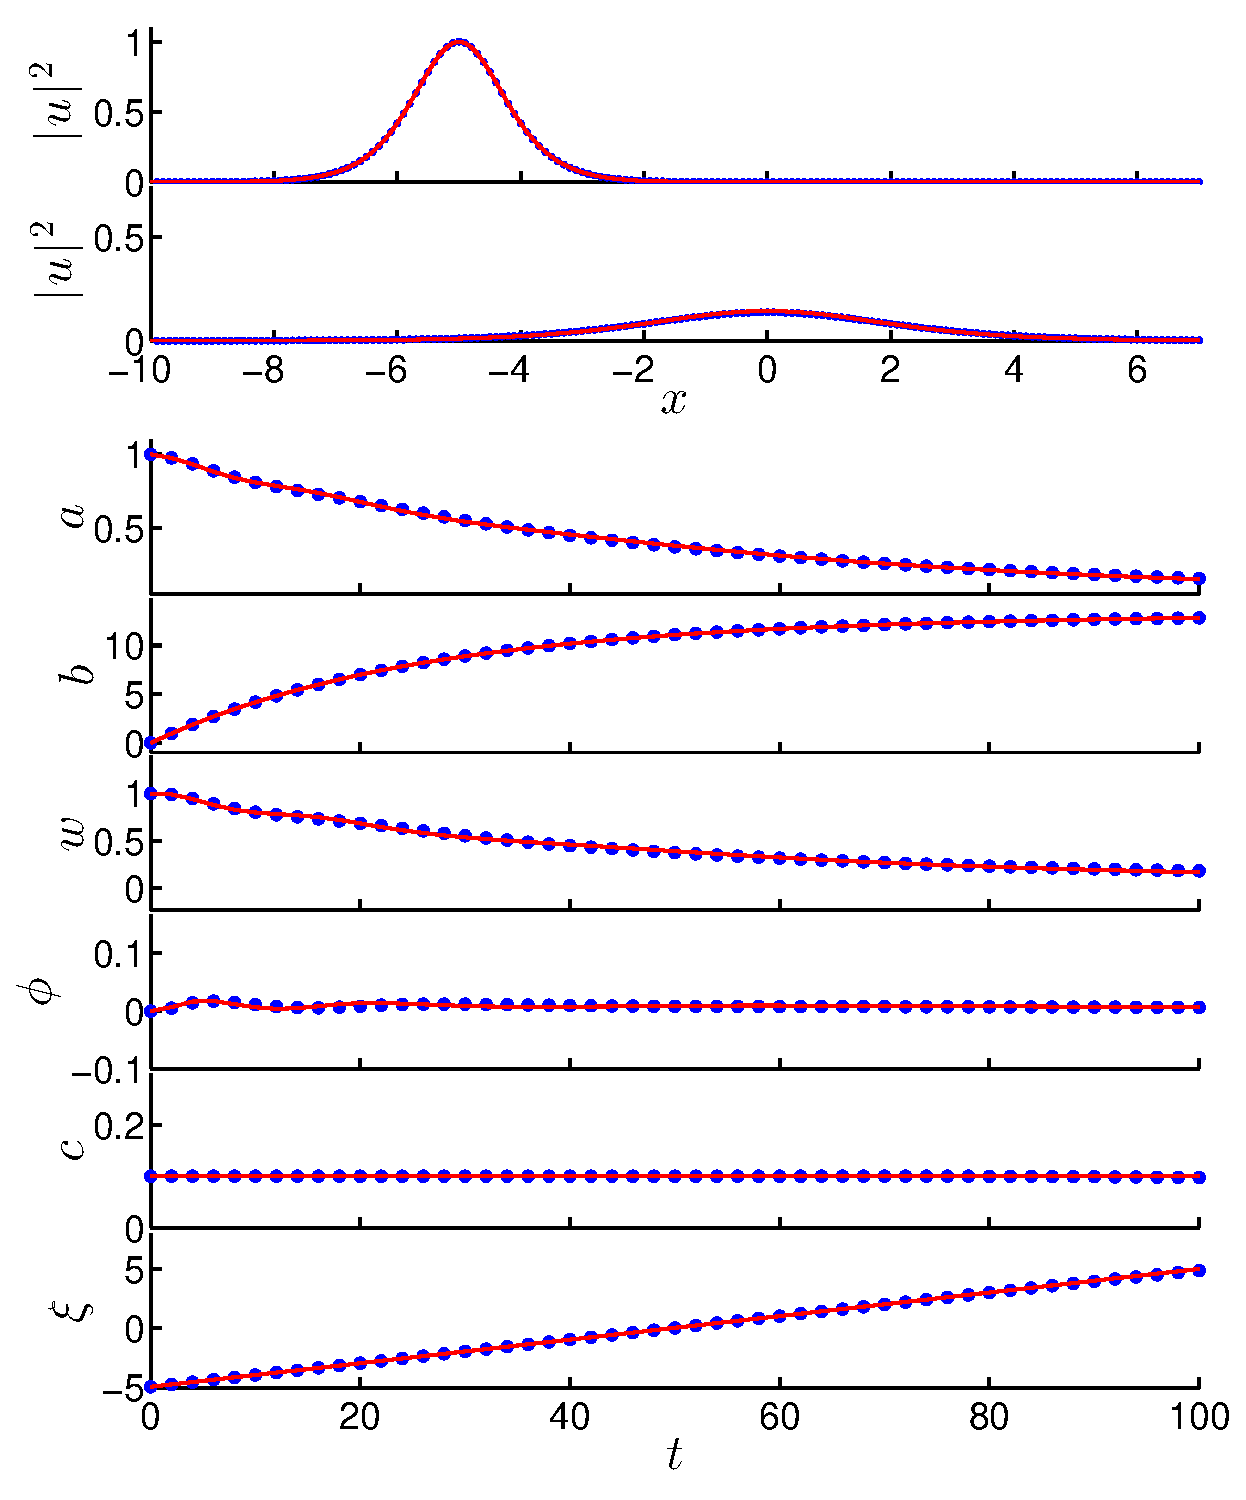
\includegraphics[width=0.8\textwidth]{fig1_LL_e001N.eps}}
  \rule{35em}{0.5pt}
  \caption[NLS with Linear Loss, $\epsilon = 0.01$]{Evolution of an NLS bright soliton under the presence of linear loss of strength $\epsilon=0.01$.  A bright soliton, as described by Eq.~(\ref{ansatz1}), is used as an initial condition with the parameters:  $a(0)=w(0)=1$, $c(0)=0.1$, $\xi(0) = -5$, and $b(0)=\phi(0)=0$.  The plots compare the NCVA approximations of Eq.~(\ref{eq:NCVALL}) (red lines) with the numerical NLS evolution of  Eq.~(\ref{eq:NLSLL}) (blue dots).  The top subpanel depicts the density $|u|^2$ at the initial time $(t=0)$.  The second subpanel depicts the density after the system is evolved for a total time of $t=1/\epsilon$.  The bottom six subpanels detail the evolution of the NCVA ansatz parameters $a$, $b$, $c$, $\xi$, $w$, and $\phi$ (red lines).  For the NLS evolution, the parameters are extracted by projecting the current solution into the NCVA ansatz using least squares fitting (blue dots).}
 \label{fig:Loss001}
\end{figure}


\begin{figure}[htbp]
  \centering
  \centerline{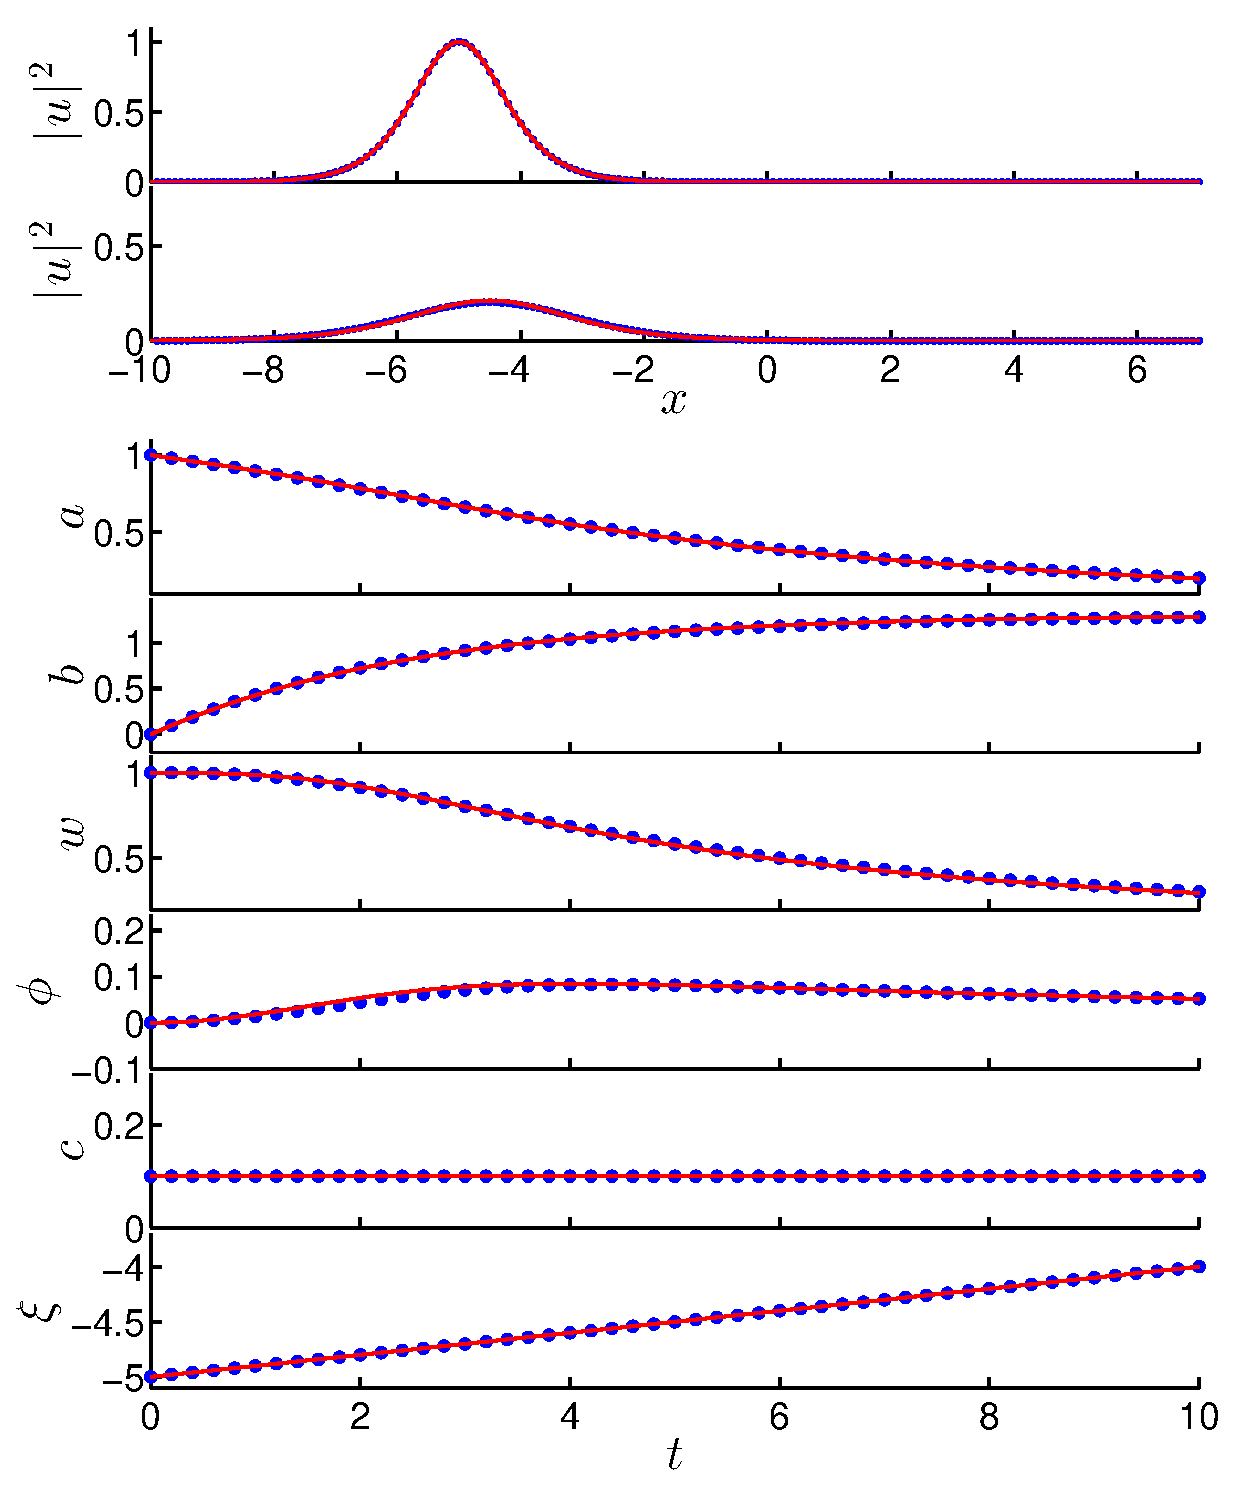
\includegraphics[width=0.8\textwidth]{fig2_LL_e01N.eps}}
  \rule{35em}{0.5pt}
  \caption[NLS with Linear Loss, $\epsilon = 0.1$]{Evolution of an NLS bright soliton under the presence of linear loss of strength $\epsilon=0.1$.  The NCVA results are obtained from Eq.~(\ref{eq:NCVALL}) (red lines) while the full numerical solution is obtained from Eq.~(\ref{eq:NLSLL}) (blue dots).  Same initial conditions and layout of panels as in the previous figure.}
 \label{fig:Loss01}
\end{figure}

\begin{figure}[htbp]
  \centering
  \centerline{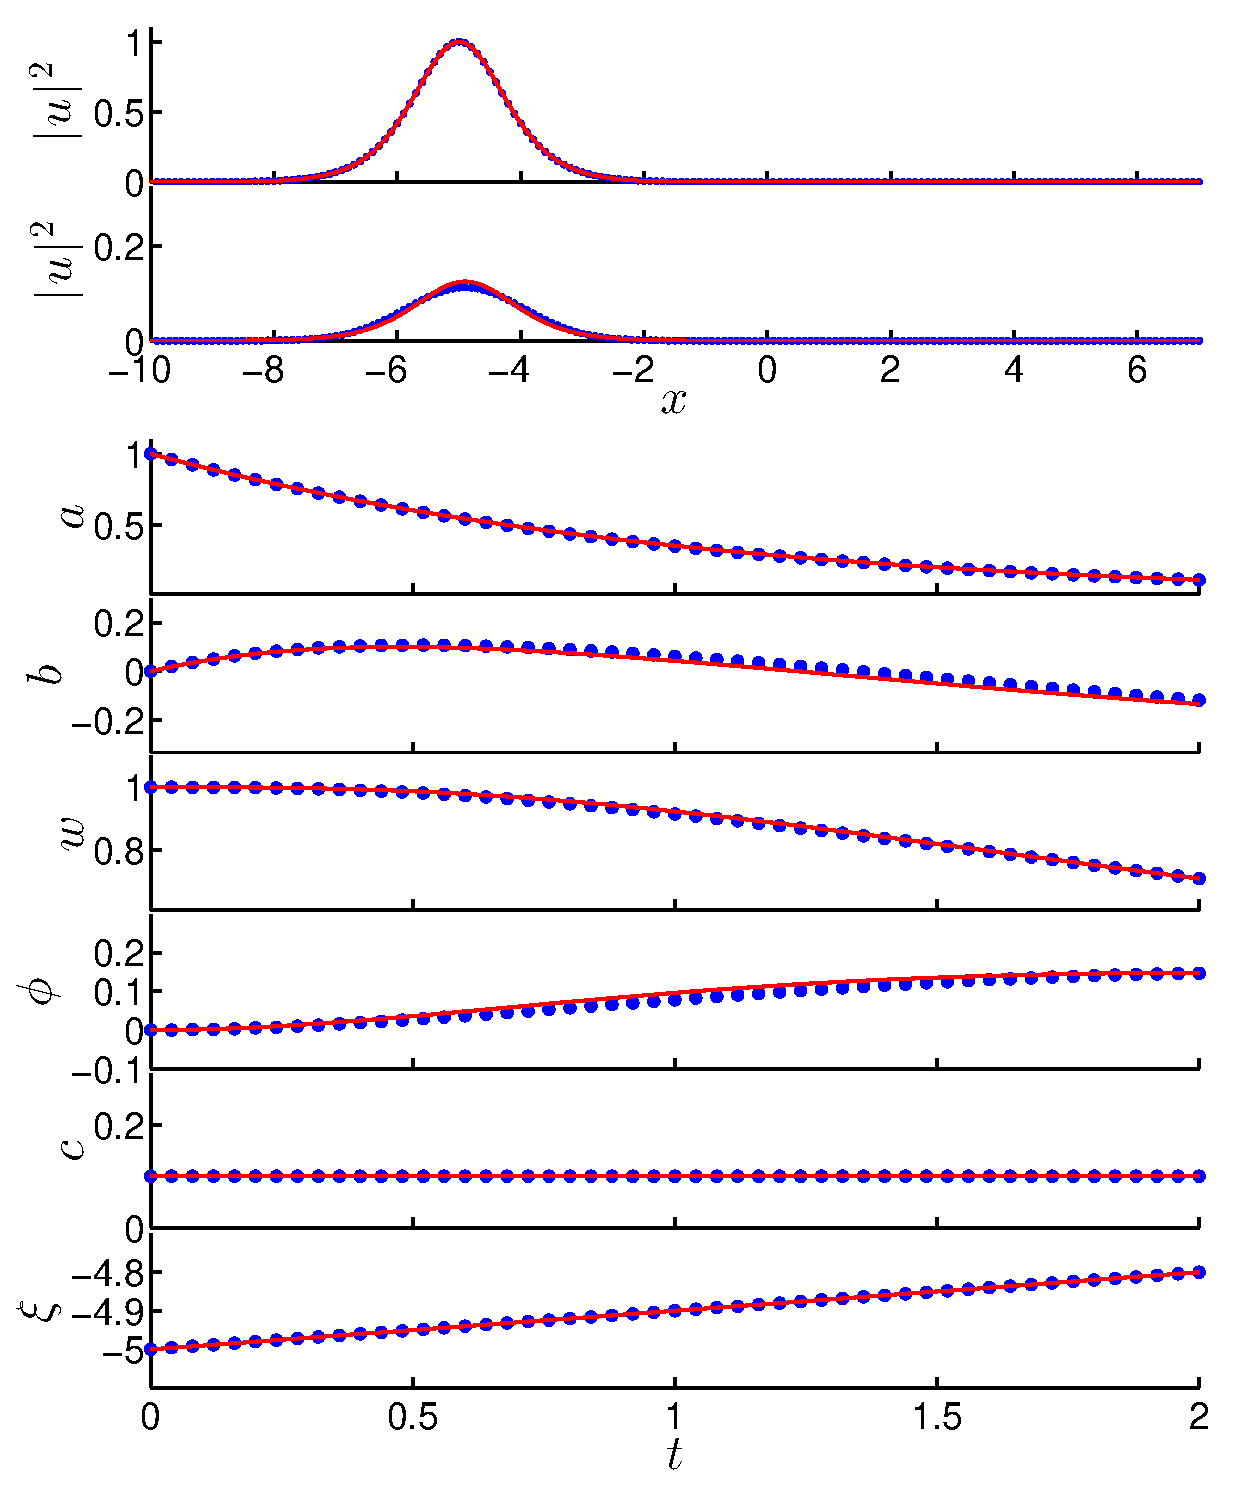
\includegraphics[width=0.8\textwidth]{Fig1b_LL_e1N.eps}}
  \rule{35em}{0.5pt}
  \caption[NLS with Linear Loss, $\epsilon = 1$]{Evolution of an NLS bright soliton under the presence of linear loss of strength $\epsilon=1$.  The NCVA results are obtained from Eq.~(\ref{eq:NCVALL}) (red lines) while the full numerical solution is obtained from Eq.~(\ref{eq:NLSLL}) (blue dots).  Same initial conditions and layout of panels as in previous figures.  The system is evolved for a total time of $t = 2/\epsilon$.}
   \label{fig:Loss1}
\end{figure}


%\begin{figure}[htbp]
%\centering
%\begin{subfigure}[t]{0.49\textwidth}
%  		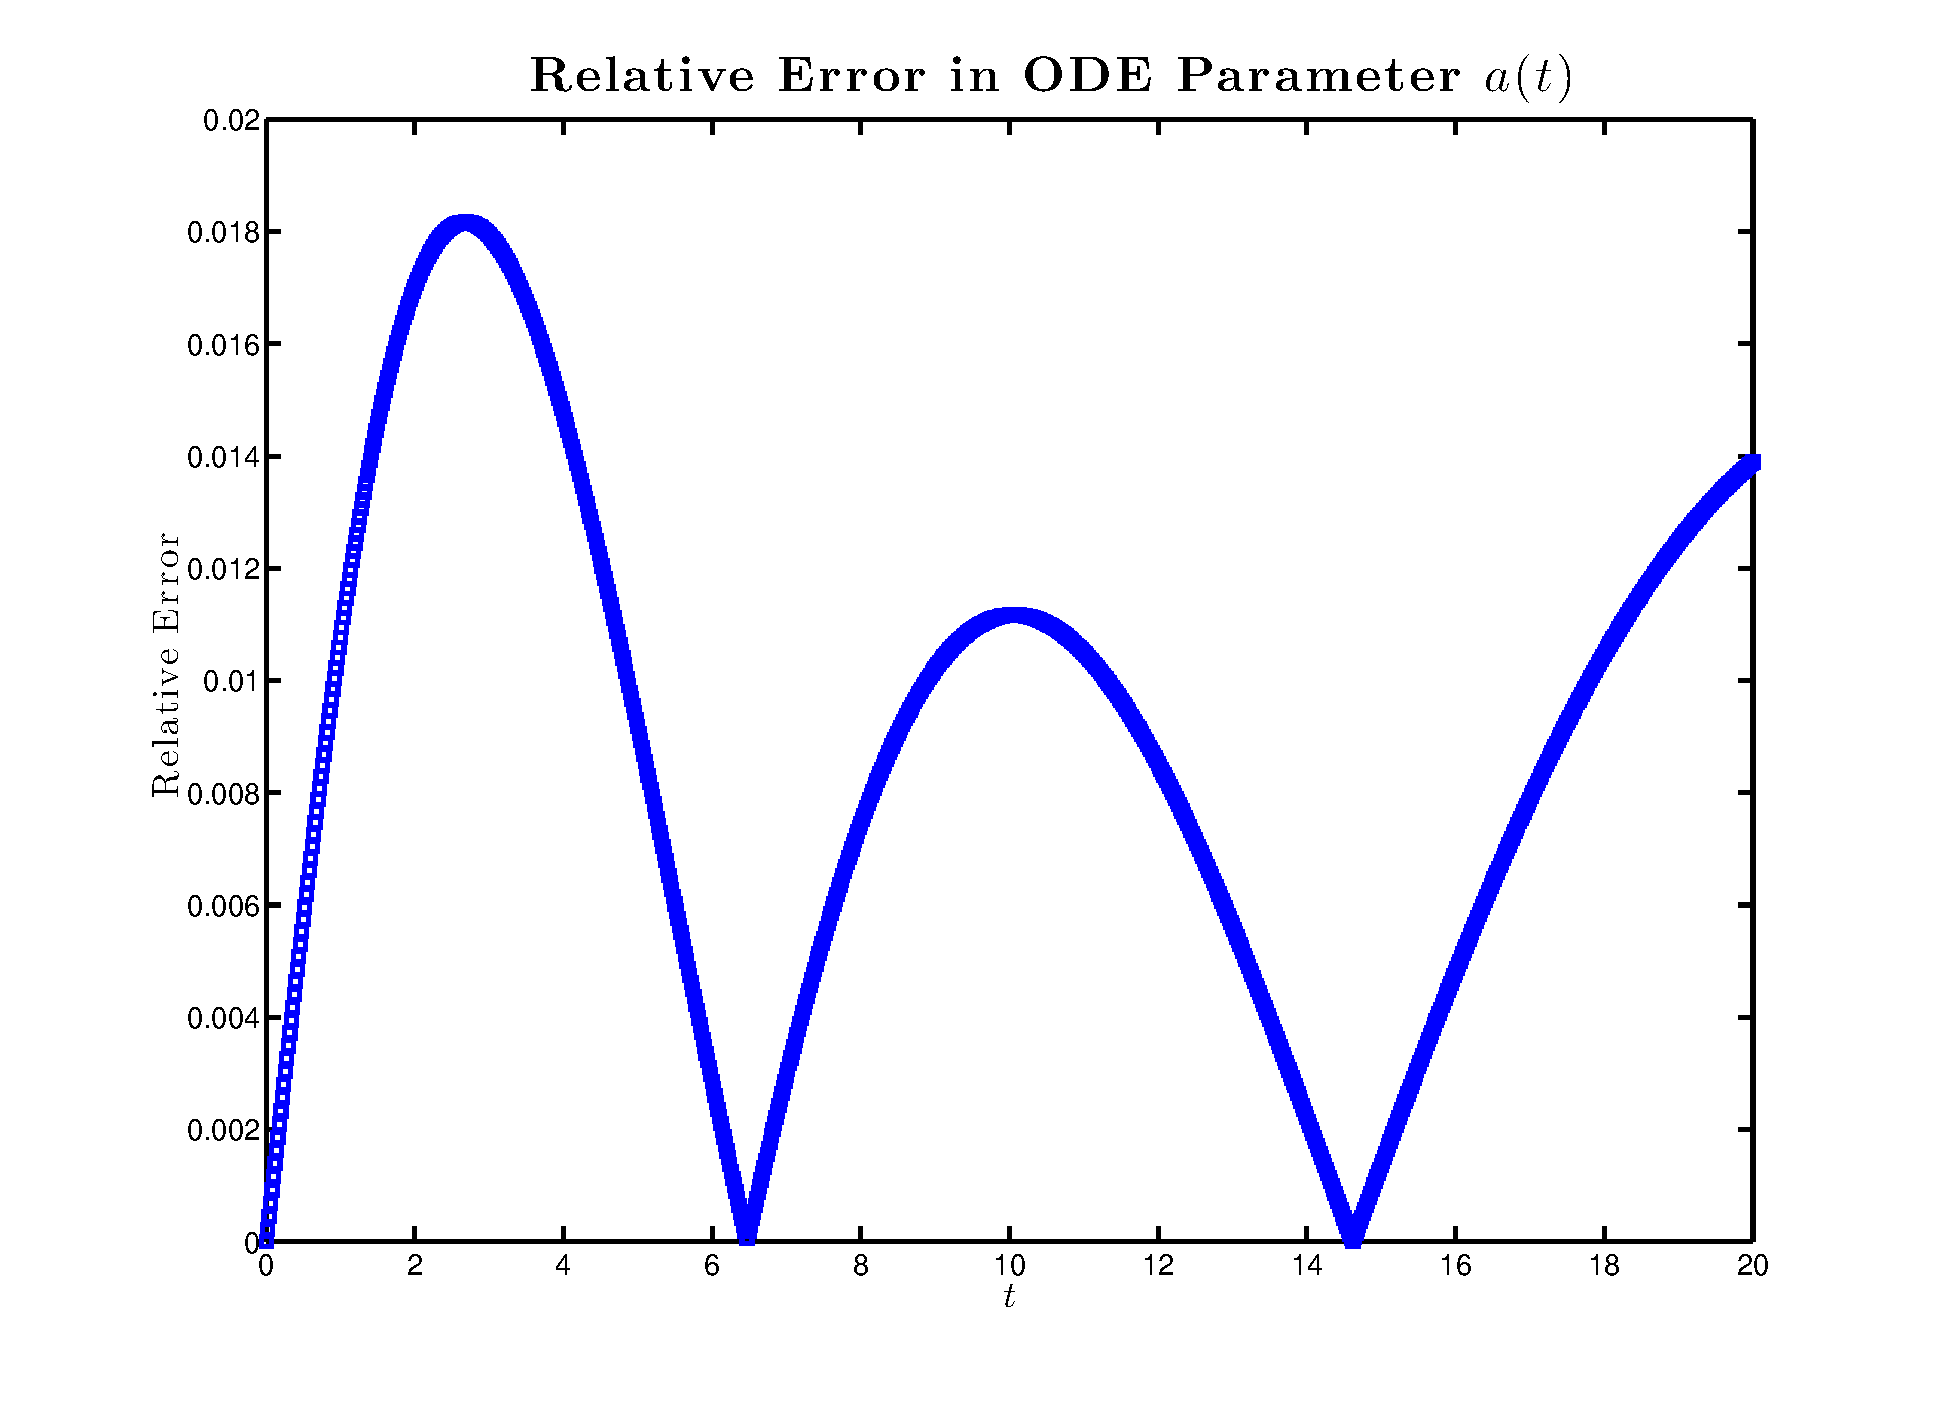
\includegraphics[width=\textwidth, height = \textwidth]{LL001relativeerror.eps}
%	         \caption{Relative error between NCVA and PDE parameter $a(t)$ values for $\epsilon=0.01$.}
%	         \label{fig:Loss001Err}
%	     \end{subfigure}
%  \begin{subfigure}[t]{0.49\textwidth}
%  		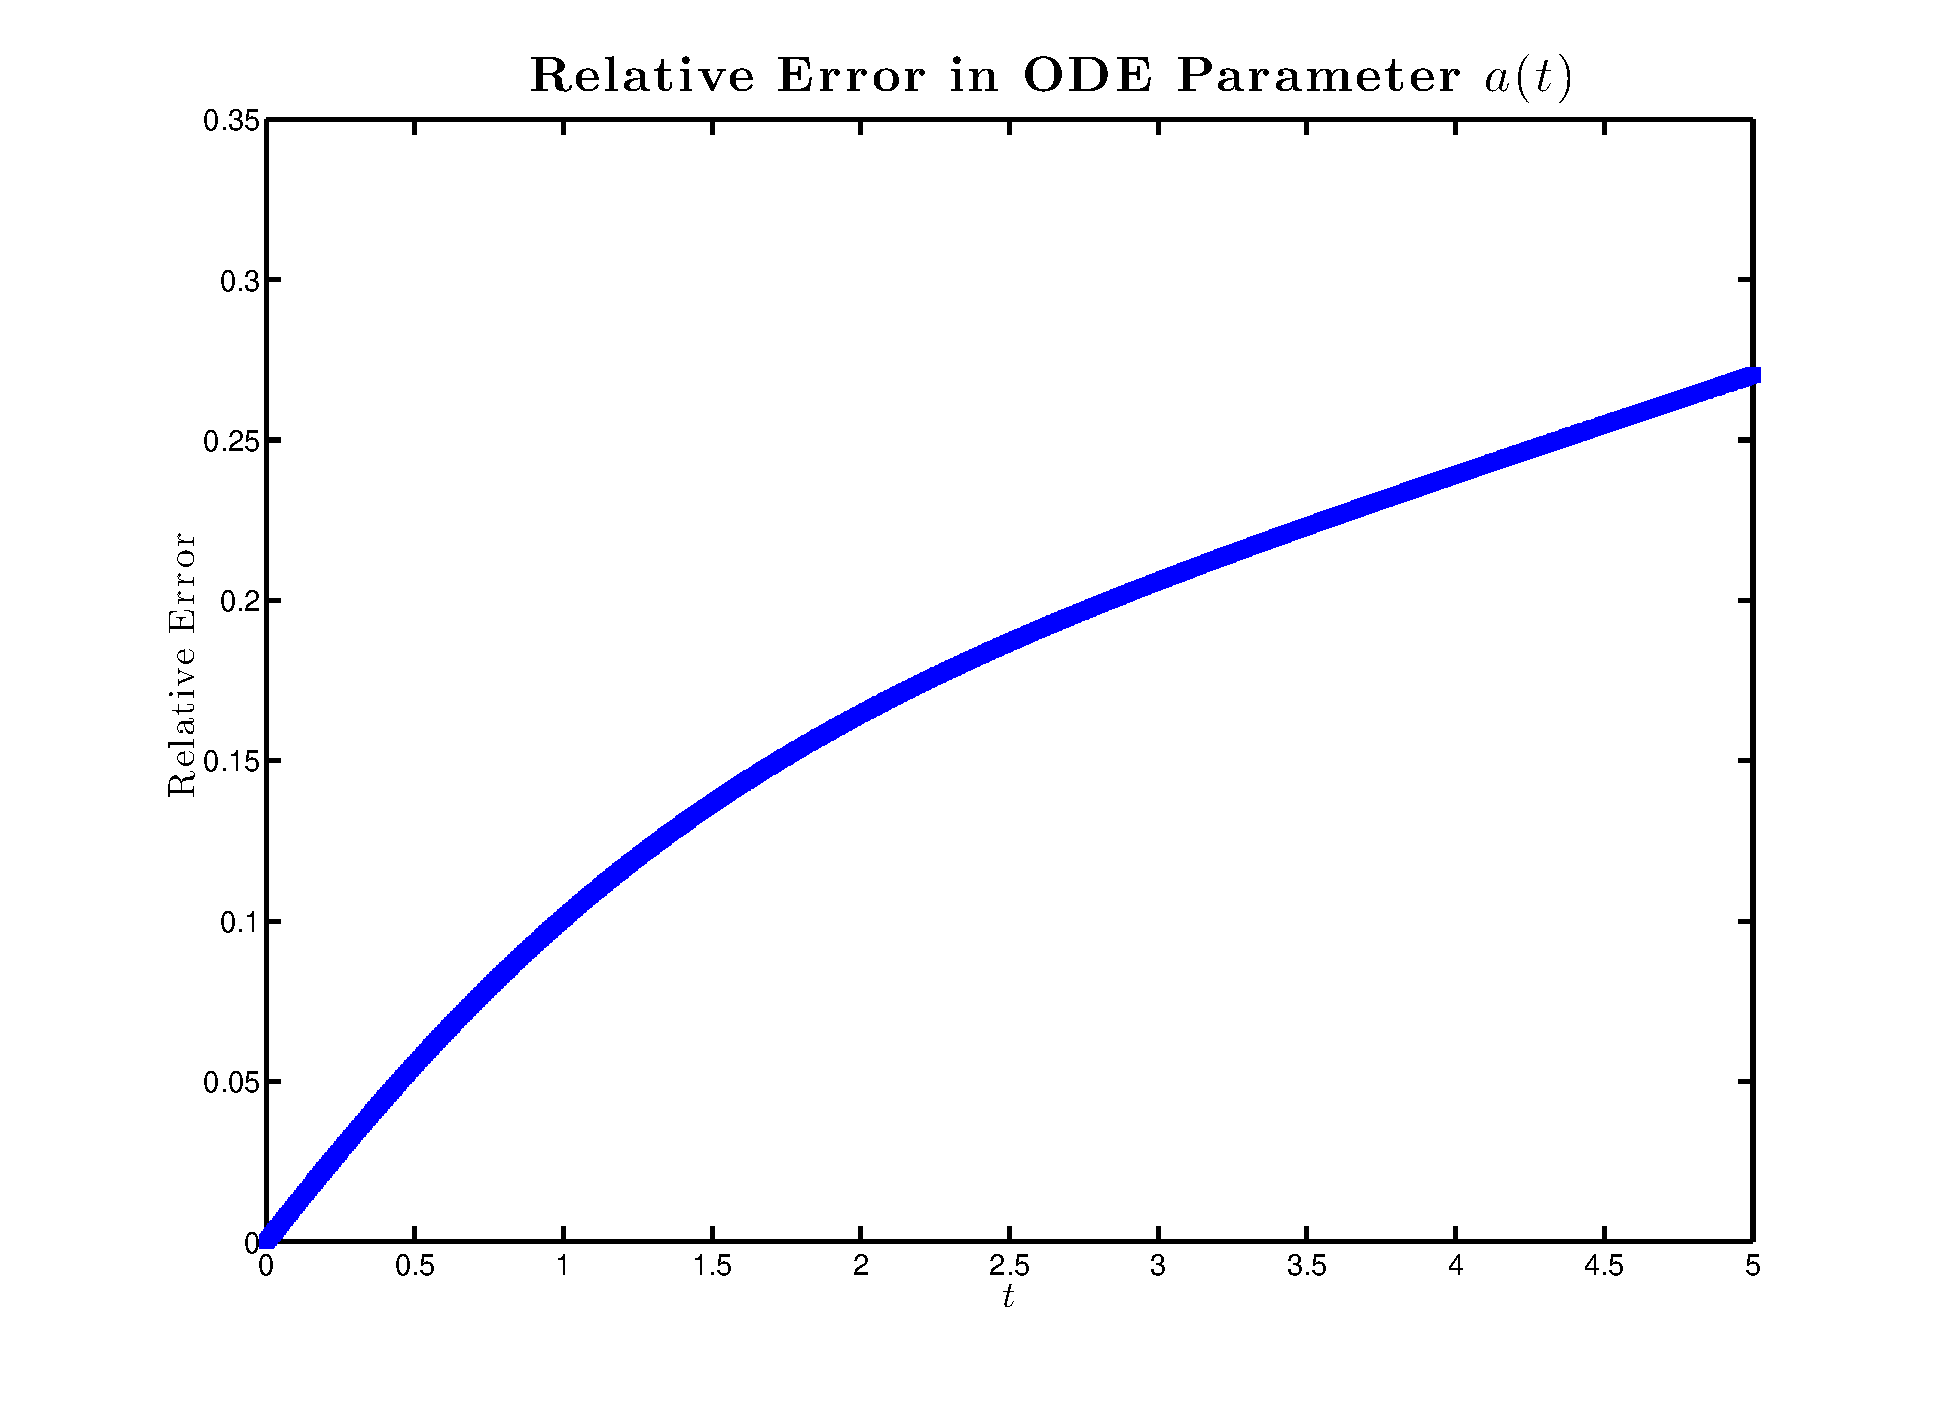
\includegraphics[width= \textwidth, height = \textwidth]{LL01relativeerror.eps}  
%	          \caption{Relative error between NCVA and PDE parameter $a(t)$ values for $\epsilon=0.1$.}
%	         \label{fig:Loss01Err}
%	    \end{subfigure} 
%  \rule{35em}{0.5pt}
%   \caption[Relative Error in Amplitude for NLS with Linear Loss]{{\bf NLS with Linear Loss:} Amplitude parameter $a(t)$ relative error for (A) $\epsilon=0.01$ and (B) $\epsilon=0.1$.}
%   \label{fig:LLossA}
%\end{figure}



%\begin{figure}[htbp]
%\centering
%\begin{subfigure}[t]{0.49\textwidth}
%  		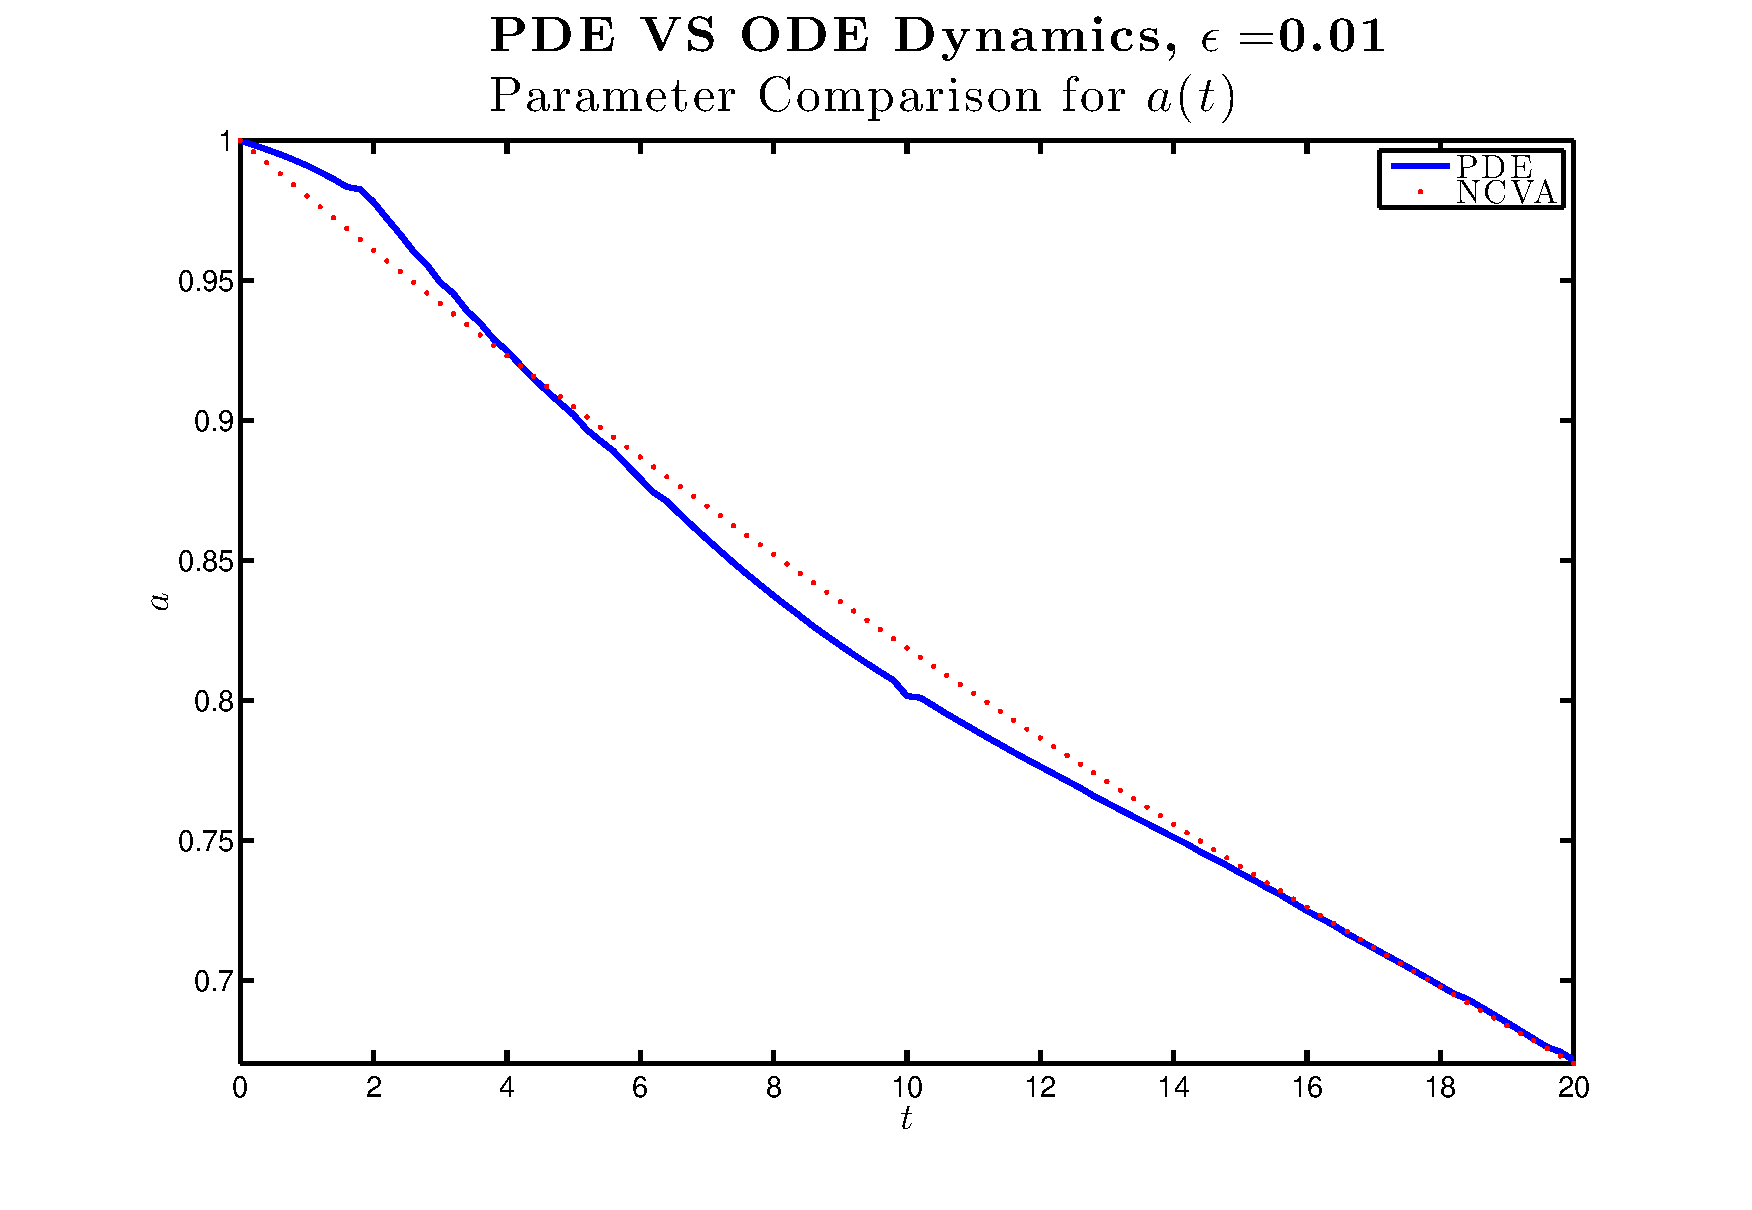
\includegraphics[width=\textwidth, height = \textwidth]{LLE001a.eps}
%	         \caption{Amplitude parameter comparison $a(t)$ between PDE and NCVA solutions.}
%	         \label{fig:Loss001a}
%	     \end{subfigure}
%  \begin{subfigure}[t]{0.49\textwidth}
%  		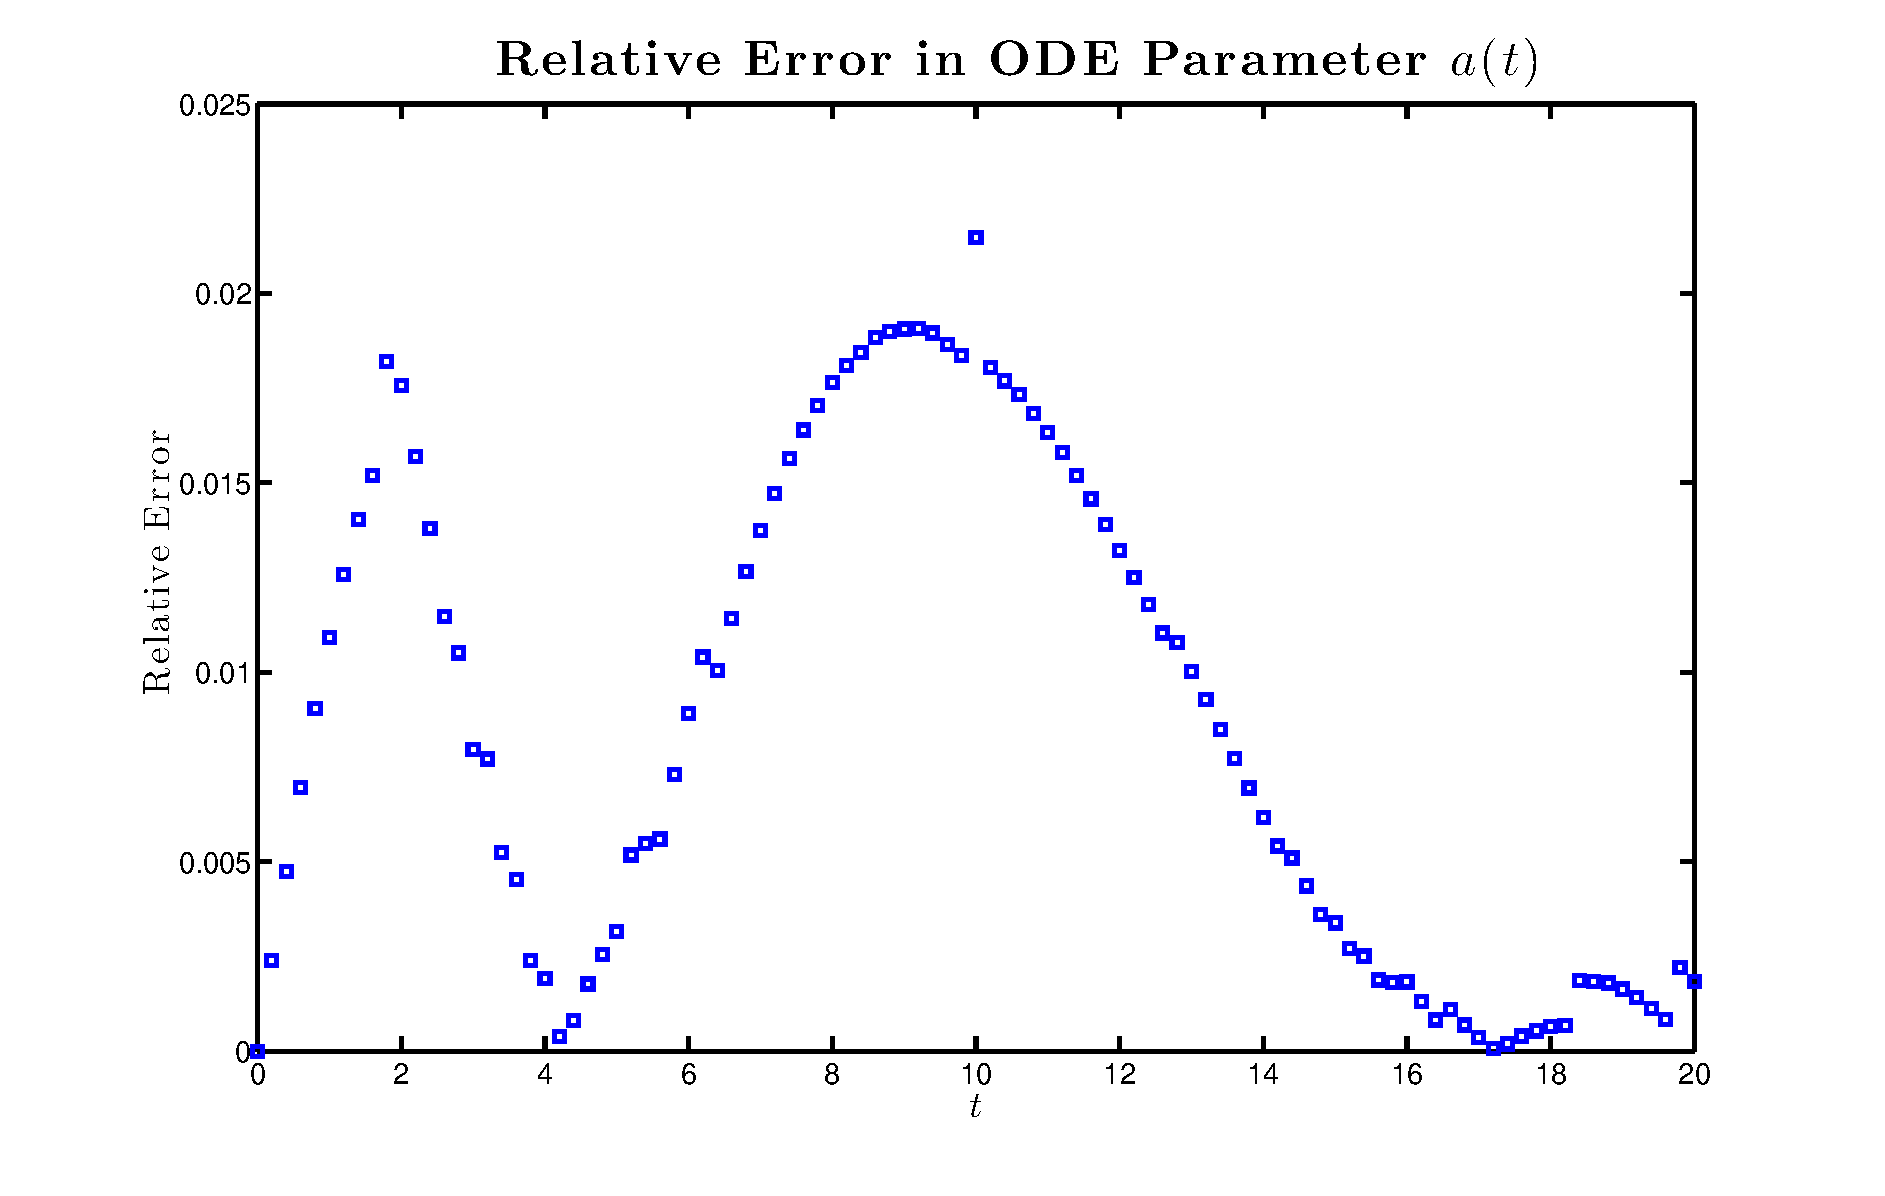
\includegraphics[width= \textwidth, height = \textwidth]{LLE001relativeError.eps}  
%	          \caption{Relative error between NCVA and PDE parameter $a(t)$ values.}
%	         \label{fig:Loss001Err}
%	    \end{subfigure} 
%  \rule{35em}{0.5pt}
%   \caption[NLS with Linear Loss, $\epsilon = 0.01$ Amplitude Comparison and Relative Error]{{\bf NLS with Linear Loss:} Amplitude parameter $a(t)$ ansatz comparisons and relative error for $\epsilon=0.01$.}
%   \label{fig:LLossA}
%\end{figure}
%
%
%\begin{figure}[htbp]
%\begin{subfigure}[b]{0.5\textwidth}
%  		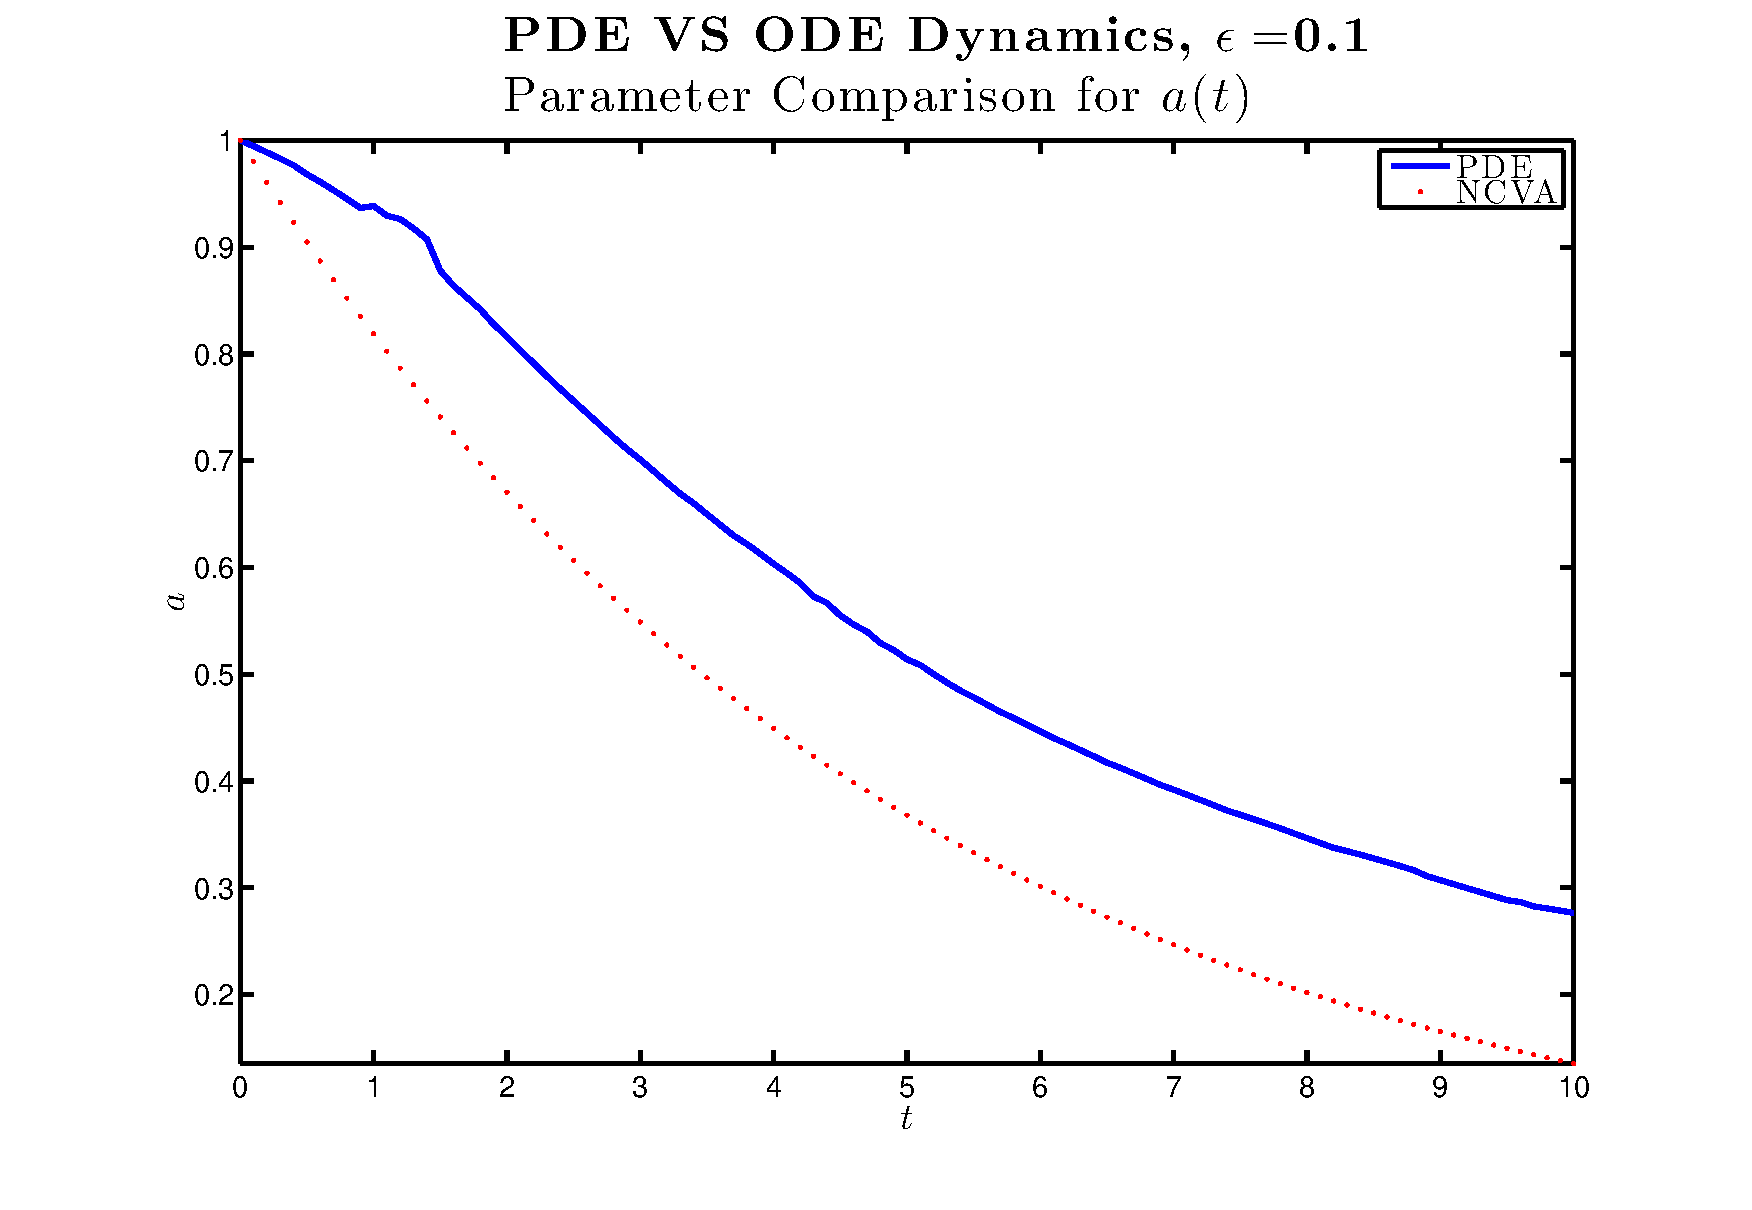
\includegraphics[width=\textwidth, height = \textwidth]{LLE01a.eps}
%	         \caption{Amplitude parameter comparison $a(t)$ between PDE and NCVA solutions.}
%	         \label{fig:Loss01a}
%	     \end{subfigure}
%  \begin{subfigure}[b]{0.5\textwidth}
%  		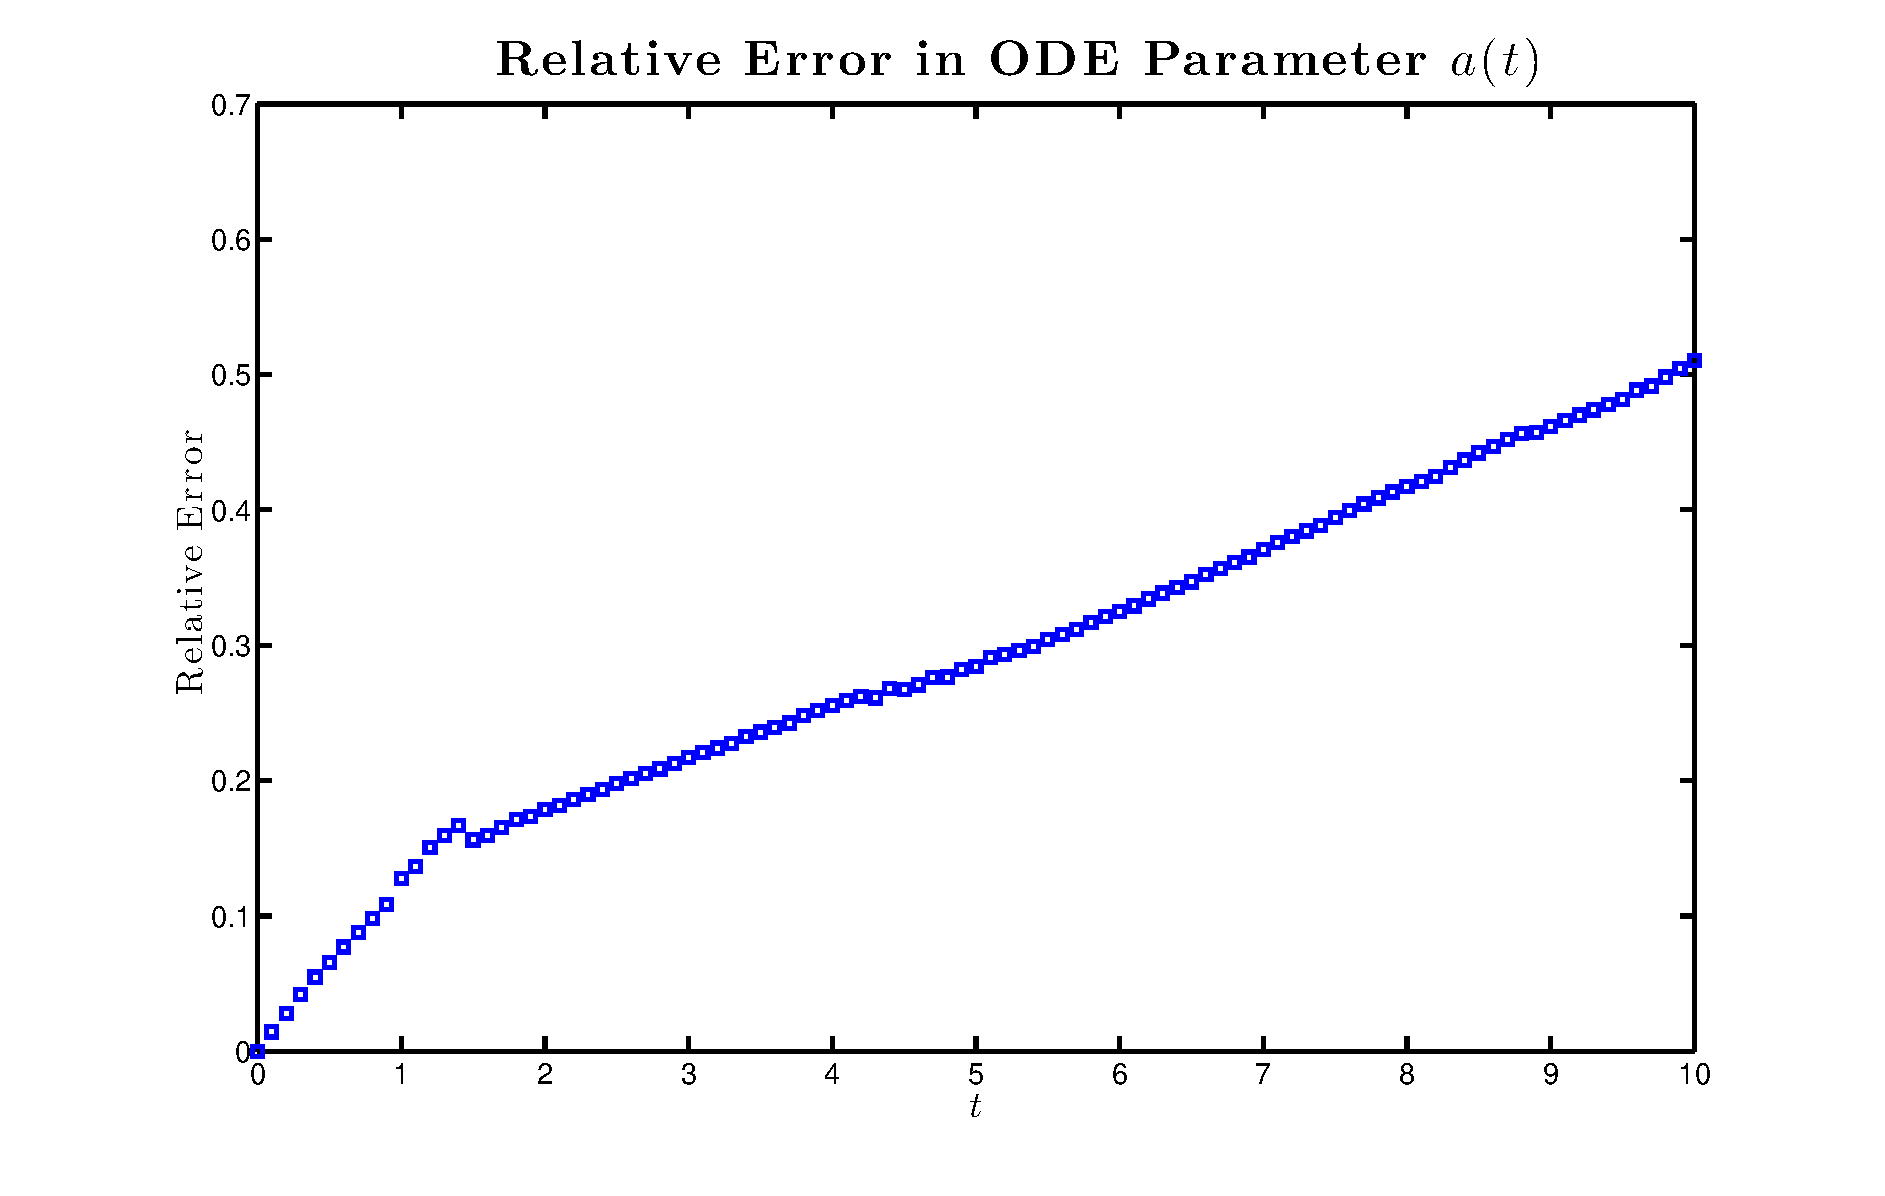
\includegraphics[width= \textwidth, height = \textwidth]{LLE01relativeError.eps}  
%	          \caption{Relative error between NCVA and PDE parameter $a(t)$ values.}
%	         \label{fig:Loss01Err}
%	    \end{subfigure} 
%  \rule{35em}{0.5pt}
%   \caption[NLS with Linear Loss, $\epsilon = 0.1$ Height Comparison and Relative Error]{{\bf NLS with Linear Loss:} Amplitude parameter $a(t)$ ansatz comparisons and relative error for $\epsilon=0.1$.}
%   \label{fig:LLossA2}
%\end{figure}

\clearpage
%%%% Section NLS with Density Dependent Loss %%%%%%%%%%%
\setstretch{1.3}
\section[Nonlinear Schr\"{o}dinger Equation with Density Dependent Loss]{NLS Equation with Density Dependent Loss}
\label{section:DDL}

\setstretch{2}
In the second dynamical system example, we use the attractive NLS equation with a density dependent (nonlinear) loss term of strength $\epsilon$:
\begin{align}
iu_t + \frac{1}{2} u_{xx} + |u|^2 u = -i  \epsilon  |u|^2 u. 
\label{eq:NLSDD}
\end{align}
The Lagrangian corresponding to the conservative problem ($\epsilon = 0$) is the same as Eq.~(\ref{eq:ConservativeL}).
% given by:
%\begin{align}
%\mathcal{L} = \frac{i}{2} \Bigg( u \frac{\partial u^*}{\partial t} -u^* \frac{\partial u}{\partial t} \Bigg) + \frac{1}{2} \Bigg| \frac{\partial u}{\partial x} \Bigg|^2  - \frac{1}{2} | u|^4.
%\end{align}
We again use the bright soliton ansatz Eq.~(\ref{ansatz1})
%\begin{align}
%u_A(x,t; \vec{p}) = a \, \mathrm{sech}[w(x-\xi)] \, \exp [i(b(x-\xi)^2+ c(x-\xi)+\phi)],
%\label{ansatz1}
%\end{align}
with a vector of time-dependent ansatz parameters given by $\vec{p} = (a, w, \xi, c, b, \phi)$.
% with arbitrary height $a$, inverse width $w$, center position $\xi$, speed $c$, chirp $b$, and phase $\phi$. 

%\subsection{Perturbed Variational Approximation}
%In the perturbed and modified Kantorovitch variational approximation methods the non-conservative term is given by 
%\begin{align}
%\mathcal{P} = \epsilon \mathcal{Q} = - i \epsilon |u|^2 u,
%\end{align}
%and the two solutions are equivalent.  
%%According to Cerda's~\cite{Cerda} method the non-conservative term is described as
%%\begin{align}
%%Q = -i\epsilon |u|^2 u,
%%\end{align}
%%and the two solutions are equivalent.
%From the modified Kantorovitch method and the perturbed variational approximation it is straightforward to obtain a system of six coupled ODEs for the ansatz parameters:
%%\begin{align} \begin{cases}
%%2 \dot{b} - a^2 - 2c\dot{\xi} + c^2 = 0, \\
%%-2\dot{a} = \frac{8}{3} \epsilon a^3, \\
%%-2\dot{\xi} a + 2ac = 0, \\
%%2 \dot{a} c + 2 a \dot{c} = -\frac{8}{3} \epsilon a^3 c. 
%%\end{cases} \end{align} 
%%The four equations are solved simultaneously to find the following system of ODEs for the NLS with density dependent loss: 
%{\setstretch{1.3} 
%\begin{align}\begin{cases}
% \dot{a} = - \frac{2}{3} \epsilon a^3   - a b - \frac{2}{\pi^2} \epsilon a^3, \\[1.0ex]
%\dot{b}  = \frac{2}{\pi^2}w^4 - \frac{2}{\pi^2}a^2 w^2 - 2 b^2, \\[1.0ex]
%\dot{c} = 0 , \\[1.0ex]
%\dot{\xi} = c, \\[1.0ex]
%\dot{w} = -2bw - \frac{4}{\pi^2} \epsilon a^2 w, \\[1.0ex]
%\dot{\phi} = \frac{5}{6} a^2 - \frac{1}{3} w^2 + \frac{1}{2} c^2,
%\end{cases} \label{eq:PVADD} \end{align}}
%\vskip -5cm

\subsection{Non-conservative Variational Approximation} \label{section:DD}
In the NCVA framework, the $\bar{u}_1$ and $\bar{u}_2$ ans\"{a}tze are defined as in Eqs.~(\ref{eq:psi1}) and (\ref{eq:psi2}).
%\begin{align}
%u_1 &= a_1 \mathrm{sech}(a_1(x-\xi_1))e^{i(c_1 (x-\xi_1)+b_1)}, \\
%u_2 &= a_2 \mathrm{sech}(a_2(x-\xi_2))e^{i(c_2 (x-\xi_2)+b_2)}.
%\end{align}
According to the non-conservative variational method the Lagrangian is $\mathcal{L}_t = \mathcal{L}_1 - \mathcal{L}_2 + \mathcal{R}$ where 
\begin{align}
\mathcal{L}_1 &= \frac{i}{2} \Big(\bar{u}_1 \bar{u}_{1,t}^* - \bar{u}_1^* \bar{u}_{1,t}\Big) + \frac{1}{2} |\bar{u}_{1,x}|^2 - \frac{1}{2}|\bar{u}_1|^4, \\
\mathcal{L}_2 &= \frac{i}{2} \Big(\bar{u}_2 \bar{u}_{2,t}^* - \bar{u}_2^* \bar{u}_{2,t}\Big) + \frac{1}{2} |\bar{u}_{2,x}|^2 - \frac{1}{2}|\bar{u}_2|^4, \\
\mathcal{P} \bar{u}_-^* &=  i\epsilon  \bar{u}_+ \bar{u}_+^* \bar{u}_+\bar{u}_-^* =  i \epsilon  \frac{(\bar{u}_1 + \bar{u}_2)}{2}\frac{(\bar{u}_1^* + \bar{u}_2^*)}{2}\frac{(\bar{u}_1 + \bar{u}_2)}{2}(\bar{u}_1 - \bar{u}_2)^*, \\
\mathcal{R} & =  i\epsilon ( \bar{u}_+ \bar{u}_+^* \bar{u}_+\bar{u}_-^* -  \bar{u}_+ \bar{u}_+^* \bar{u}_-\bar{u}_+^*).  
\end{align}
Plugging the ans\"{a}tze into $\mathcal{L}_1$ and $\mathcal{L}_2$ and integrating gives $\bar{L}_1$ and $\bar{L}_2$ of the same form as Eq.~({\ref{eq:intLi}).
%\begin{align}
%L_1 =& a_1^2 \mathrm{sech}^2(a_1(x-\xi_1))[\dot{c}_1 (x-\xi_1)-c_1\dot{\xi}_1 + \dot{b}_1] + \frac{1}{2}a_1^4 \mathrm{sech}^2(a_1(x-\xi_1))\mathrm{tanh}^2(a_1(x-\xi_1)) \nonumber \\
%&+\frac{1}{2}a_1^2c_1^2 \mathrm{sech}^2(a_1(x-\xi_1))-\frac{1}{2}a_1^4 \mathrm{sech}^4(a_1(x-\xi_1)), \\
%L_2 =& a_2^2 \mathrm{sech}^2(a_2(x-\xi_2))[\dot{c}_2 (x-\xi_2)-c_2\dot{\xi}_2 + \dot{b}_2] + \frac{1}{2}a_2^4 \mathrm{sech}^2(a_2(x-\xi_2))\mathrm{tanh}^2(a_2(x-\xi_2)) \nonumber \\
%&+\frac{1}{2}a_2^2c_2^2 \mathrm{sech}^2(a_2(x-\xi_2))-\frac{1}{2}a_2^4 \mathrm{sech}^4(a_2(x-\xi_2)).  
%\end{align}
%Next we find $\bar{L} = \int\mathscr{L}dx = \int L_1 dx - \int L_2 dx + \int R dx$, which for $L_1$ and $L_2$ is the same as with the conservative variational approximation.  The first two integrals are
%\begin{align}
%\int_{-\infty}^{\infty} L_1 dx &= 2\dot{b}_1 a_1 - \frac{1}{3}a_1^3 + c_1^2 a_1 - 2c_1 \dot{\xi}_1 a_1,  \\
%\int_{-\infty}^{\infty} L_2 dx &= 2\dot{b}_2 a_2 - \frac{1}{3}a_2^3 + c_2^2 a_2 - 2c_2 \dot{\xi}_2 a_2.
%\end{align}
%The solution for the non-conservative density dependent loss term in the effective Lagrangian is an integral of the form
%\begin{align}
%\int_{-\infty}^{\infty} \mathcal{R} dx &=   \\
% &  \frac{i}{4} \epsilon  \int & \Big( |u_1|^2( u_2u_1^* - u_2^* u_1) +  |u_2|^2( u_2u_1^* - u_2^* u_1)  + u_2u_2 u_1^*u_1^* - u_1u_1u_2^*u_2^*\Big)dx. \nonumber
%\end{align}
For the non-conservative terms, we take derivatives with respect to $p_-$ at the physical limit ($\mathrm{PL}$) and then integrate: 
\begin{align} 
\bar{R} = &  \int_{-\infty}^{\infty} \bar{\mathcal{R}} dx \nonumber \\
%\int \Big[ \frac{\partial R}{\partial p_-} \Big]_{\mathrm{PL}} dx  \nonumber \\ 
=&  \frac{i }{4} \epsilon \int \Big[ \frac{\partial}{\partial p_-} \Big(|u_1|^2( u_2u_1^* - u_2^* u_1) +  |u_2|^2( u_2u_1^* - u_2^* u_1)  + u_2u_2 u_1^*u_1^* - u_1u_1u_2^*u_2^*\Big) \Big]_{\mathrm{PL}} dx.   
\end{align}
%Putting everything back together we obtain the modified Euler-Lagrange equations:
%\begin{align}
%\frac{\partial \bar{L}}{\partial p} - \frac{d}{dt} \Bigg( \frac{\partial \bar{L} }{\partial\dot{p}}\Bigg) + \int_{-\infty}^{\infty} \Big[ \frac{\partial \bar{\mathcal{R}}}{\partial p_-} \Big]_{\mathrm{PL}} dx = 0. 
%\end{align}
Therefore, the total effective Lagrangian, $\bar{L} = \bar{L}_1 - \bar{L}_2 + \bar{R}$ is given by:
\begin{align} 
\bar{L} =& 2\frac{a_1^2  \dot{\phi}_1}{w_1}+\frac{a_1^2 c_1^2}{w_1} - 2 \frac{a_1^2 c_1 \dot{\xi}_1}{w_1} - \frac{2}{3} \frac{a_1^4}{w_1} +\frac{1}{3} a_1^2 w_1 + \frac{\pi^2}{3} \frac{ a_1^2 b_1^2}{w_1^3} + \frac{\pi^2}{6} \frac{a_1^2 \dot{b}_1}{w_1^3}  \nonumber \\
&- 2\frac{a_2^2  \dot{\phi}_2}{w_2}-\frac{a_2^2 c_2^2}{w_2} + 2 \frac{a_2^2 c_2 \dot{\xi}_2}{w_2} + \frac{2}{3} \frac{a_2^4}{w_2} -\frac{1}{3} a_2^2 w_2 - \frac{\pi^2}{3} \frac{ a_2^2 b_2^2}{w_2^3} - \frac{\pi^2}{6} \frac{a_2^2 \dot{b}_2}{w_2^3} \nonumber \\
&+ \frac{i}{4} \epsilon \int \Big[ \frac{\partial}{\partial p_-} \Big(|u_1|^2( u_2u_1^* - u_2^* u_1) +  |u_2|^2( u_2u_1^* - u_2^* u_1)  + u_2u_2 u_1^*u_1^* - u_1u_1u_2^*u_2^*\Big) \Big]_{\mathrm{PL}} dx . 
\end{align}

For all the parameters, we substitute the $\pm$ coordinates into the expression for the total effective Lagrangian $\bar{L}$.
% = \bar{L}_{C} + \bar{L}_{NC}$ where $\bar{L}_C$ is the same as in Eq.~(\ref{barLC}) and :
%\begin{align} 
%\bar{L} =& 2\Bigg[  \Bigg(\frac{2\dot{b}_+ +\dot{ b}_-}{2}\Bigg)\Bigg(\frac{2a_+ + a_-}{2}\Bigg) - \Bigg(\frac{2\dot{b}_+ - \dot{b}_-}{2}\Bigg)\Bigg(\frac{2a_+ - a_-}{2}\Bigg) \Bigg] \nonumber \\
%&+ \frac{1}{3} \Bigg[ \Bigg(\frac{2a_+ - a_-}{2} \Bigg)^3 - \Bigg(\frac{2a_+ - a_-}{2} \Bigg)^3   \Bigg] \nonumber \\
%&+ \Bigg[ \Bigg(\frac{2c_+ + c_-}{2} \Bigg)^2\Bigg(\frac{2a_+ + a_-}{2} \Bigg) -    \Bigg(\frac{2c_+ - c_-}{2} \Bigg)^2\Bigg(\frac{2a_+ -a_-}{2} \Bigg)  \Bigg] \nonumber \\
%&+ 2 \Bigg[\Bigg(\frac{2c_+ - c_-}{2} \Bigg)\Bigg(\frac{2\dot{\xi}_+ - \dot{\xi}_-}{2} \Bigg)\Bigg(\frac{2a_+ + a_-}{2} \Bigg) - \Bigg(\frac{2c_+ + c_-}{2} \Bigg)\Bigg(\frac{2\dot{\xi}_+ + \dot{\xi}_-}{2} \Bigg)\Bigg(\frac{2a_+ + a_-}{2} \Bigg) \Bigg]  \nonumber \\
%\bar{L}_{NC} =   \frac{i}{4} \epsilon \int \Big[ \frac{\partial}{\partial p_-} \Big(|u_1|^2( u_2u_1^* - u_2^* u_1) +  |u_2|^2( u_2u_1^* - u_2^* u_1)  + u_2u_2 u_1^*u_1^* - u_1u_1u_2^*u_2^*\Big) \Big]_{\mathrm{PL}} dx. 
%\end{align} 
From the $\bar{L}_1$ and $\bar{L}_2$ conservative terms we recover the standard soliton evolution equations [see Eq.~(\ref{eq:CODEsNLS})], so we just need to obtain the non-conservative ones.
%{\textit i.e.} variational approximation of NLS with the following equations of motion (ODEs):
%\[\begin{cases}
%\dot{a}  = 0 \\
%\dot{b}  = \frac{1}{2}a^2 + \frac{1}{2} c^2 \\
%\dot{c} = 0  \\
%\dot{\xi} = c
%\end{cases}\] 
From the non-conservative term $\bar{R}$, we expand in the $\pm$ coordinate systems and find the integrals:
\begin{eqnarray}
\int_{-\infty}^{\infty} \left[ \frac{\partial  \bar{\mathcal{R}}}{\partial a_-} \right]_{\rm PL} dx &=& 0,  \nonumber  \\
\int_{-\infty}^{\infty} \left[ \frac{\partial  \bar{\mathcal{R}}}{\partial b_-} \right]_{\rm PL} dx &=& -\frac{2\pi^2\epsilon}{9}  \frac{a^4}{w^3} + \frac{4\epsilon}{3} \frac{a^4}{w^3}, \nonumber \\
\int_{-\infty}^{\infty} \left[ \frac{\partial  \bar{\mathcal{R}}}{\partial c_-} \right]_{\rm PL} dx &=& 0, \nonumber \\
\int_{-\infty}^{\infty} \left[ \frac{\partial  \bar{\mathcal{R}}}{\partial \xi_-} \right]_{\rm PL} dx &=&  \frac{8\epsilon}{3}   \frac{a^4 c }{w},\nonumber \\
\int_{-\infty}^{\infty} \left[ \frac{\partial  \bar{\mathcal{R}}}{\partial w_-} \right]_{\rm PL} dx &=& 0, \nonumber \\
\int_{-\infty}^{\infty} \left[ \frac{\partial  \bar{\mathcal{R}}}{\partial \phi_-} \right]_{\rm PL} dx &=&  -\frac{8\epsilon}{3}   \frac{a^4}{w}.\nonumber
\end{eqnarray}
%\begin{align}
%\int \Big[ \frac{\partial R}{\partial a_-} \Big]_{\mathrm{PL}} dx &= 0,  \nonumber  \\
%\int \Big[ \frac{\partial R}{\partial b_-} \Big]_{\mathrm{PL}} dx &= -\frac{8}{3}  \epsilon a^3, \nonumber \\
%\int \Big[ \frac{\partial R}{\partial c_-} \Big]_{\mathrm{PL}} dx &= 0, \nonumber \\
%\int \Big[ \frac{\partial R}{\partial \xi_-} \Big]_{\mathrm{PL}} dx &=  \frac{8}{3}  \epsilon a^3 c. \nonumber 
%\end{align}
%The total Lagrangian $\bar{L}$ has the system of equations:
%\begin{align} 
%2\dot{b} - a^2 -2c\dot{\xi} +c^2  &= 0, \nonumber \\ 
%-2\dot{a} - \frac{8}{3} \epsilon a^3 &= 0, \nonumber \\ 
%2a(-\dot{\xi}+c) &= 0, \nonumber \\ 
%2\dot{a}c+2a\dot{c} + \frac{8}{3} \epsilon a^3 c &=  0.\nonumber 
%\end{align}
Combining the conservative and non-conservative contributions, the equations of motion from the NCVA for the NLS with density dependent loss are the following:
%
{\setstretch{1.5} 
\begin{equation}
\begin{cases}
  \dot{a} = - \frac{2}{3} \epsilon a^3   - a b - \frac{2}{\pi^2} \epsilon a^3, \\[1.0ex]
\dot{b}  = \frac{2}{\pi^2}w^4 - \frac{2}{\pi^2}a^2 w^2 - 2 b^2, \\[1.0ex]
\dot{c} = 0 , \\[1.0ex]
\dot{\xi} = c, \\[1.0ex]
\dot{w} = -2bw - \frac{4}{\pi^2} \epsilon a^2 w, \\[1.0ex]
\dot{\phi} = \frac{5}{6} a^2 - \frac{1}{3} w^2 + \frac{1}{2} c^2, \end{cases}
 \label{eq:NVCADD}
 \end{equation}}
% \begin{align}
% \begin{cases} \dot{a} = - \frac{4}{3} \epsilon a^3, \\ 
%\dot{b} = \frac{1}{2} a^2 + \frac{1}{2} c^2, \\
% \dot{c} = 0, \\ 
% \dot{\xi} = c.  \end{cases} 
% \label{eq:NVCADD}
% \end{align}
which correspond to the same dynamics as the conservative case (\ref{eq:CODEsNLS}) with the
added nonlinear loss terms $-(2/3 + 2/\pi^2 )\epsilon a^3$ for the evolution of the amplitude
and $-4/\pi^2 \epsilon a^2 w$ for the evolution of the inverse width.  
%The equations of motion arising from the perturbed/Kantorovitch variational approximations [Eq.~(\ref{eq:PVADD})] and the NCVA [Eq.~(\ref{eq:NVCADD})] are equivalent.
 
%%Numerical Results - DD
\subsection{Numerical Results: NLS with Density Dependent Loss}
Figure~\ref{fig:DDloss01} depicts a numerical comparison between full integration of the NLS with density dependent loss and the NCVA [Eq.~(\ref{eq:NVCADD})] for $\epsilon = 0.1$.  The same numerical approach, ansatz and initial conditions were taken as in Sect.~\ref{section:LLnumerics}.  
%For $\epsilon$ = 0.01, the same spatial and temporal discretization was used as the linear loss test case for temporal domain $t\in[0,20]$.  
For $\epsilon$ = 0.1, the numerical integration temporal domain was changed to $t\in[0,10]$, with the same discretization $dx$ = 0.05 and $dt$ = 0.001.


%For the equations of motion in the NCVA (Equation~\ref{eq:NVCADD}), I used \texttt{ode45} using variable step Runge-Kutta method to solve the differential equations (ODEs) numerically.  The comparison between the ODE and PDE solution parameters $a$, $b$, $c$, and $\xi$ are plotted as functions of time.  In order to compare the PDE solution to the ODEs, the PDE solution is projected onto the ODE ansatz at discrete time intervals.  The ODE ansatz is of the form 
%\[
%u(x,t) =  a \mathrm{sech}(a(x-\xi))e^{i(c(x-\xi)+b)}
%\label{eqn:ansatz1}
%\] 
%such that the PDE integrated solutions are fit to the ansatz using \texttt{nlinfit}.  The initial conditions are $a_0 = 1$, $c_0 = 0.5$, $b_0= 0$, and $\xi_0 = -5$ to give an initial ansatz
%\[ 
%u(x, t=0) =  \mathrm{sech}(x+5)e^{i(0.5(x+5))}.
%\]
%In the PDE integration for linear loss given $\epsilon = 0.01$, the spatial domain is $x\in [-40,40]$ with spatial step size $dx = 0.01$ and $dt=0.0001$ for temporal domain $t\in[0,20]$ in Figure~\ref{fig:DDloss001}.  In the PDE integration for linear loss given $\epsilon = 0.1$, the parameters were all the same except the temporal domain $t\in[0,10]$ in Figure~\ref{fig:DDloss01}, since the soliton solution dissipates quickly.  To quantify the comparison between the ODE and PDE solution, I plotted the relative error of the parameter $a(t)$ of the ODE with respect to the PDE solution.  The $a$ parameter comparison between the NCVA ODEs and the relative error between the NCVA ODEs and the PDE are shown in Figures~\ref{fig:DDlossA} and~\ref{fig:DDlossA2} for $\epsilon = 0.01$ and 0.1, respectively.  

Similar to linear loss, the density dependent loss NCVAs are in good agreement to the full NLS dynamics even in the presence of a nonlinear loss.  In general, the dynamics of the PDE solution agrees well with the parameters in the coupled ODEs that fit to the ansatz.  The speed $c$ is constant in time and $\xi(t) = c\,t$ as a linear increase in the test cases.  The chirp parameter $b$ has more complex dynamics in agreement between the PDE and ODEs.  The main discrepancy between the PDE and the ODE is that the dissipation of the height $a$, described by $\dot{a} = -\frac{4}{3} \epsilon a^3$ in the NCVA, follows a power law rather than an exponential as expected. 

% For larger $\epsilon$, the NCVA height is an approximation of the true solution within a close tolerance with relative error on the order of $10^{-3}$ (see Fig.~\ref{fig:DLoss001Err}).  For larger perturbation, $\epsilon$ = 0.1 the NCVA approximation is less accurate with a relative error on the order of $10^{-2}$ (see Fig.~\ref{fig:DLoss01Err}).  
% For $\epsilon$ = 0.01, the NCVA approximates very well the true NLS soliton.  This basic dynamical system gives us a good example of the differences through comparison of the equation of motions for the ODEs and the NLS.  Mainly the ODEs have $\dot{c} = 0$ and $\dot{a} = -\frac{4}{3} \epsilon a(t)^3$; however, as seen in Figs.~\ref{fig:DDloss001} and~\ref{fig:DDloss01}, the PDE solution fluctuates around a constant $c$ parameter but not as perfectly as the ODE solution.  The ODE solution for $a$ parameter is cubic, but fails to follow the curvature of the PDE solution for amplitude.  
 
 \begin{figure}[htbp]
  \centering
  \centerline{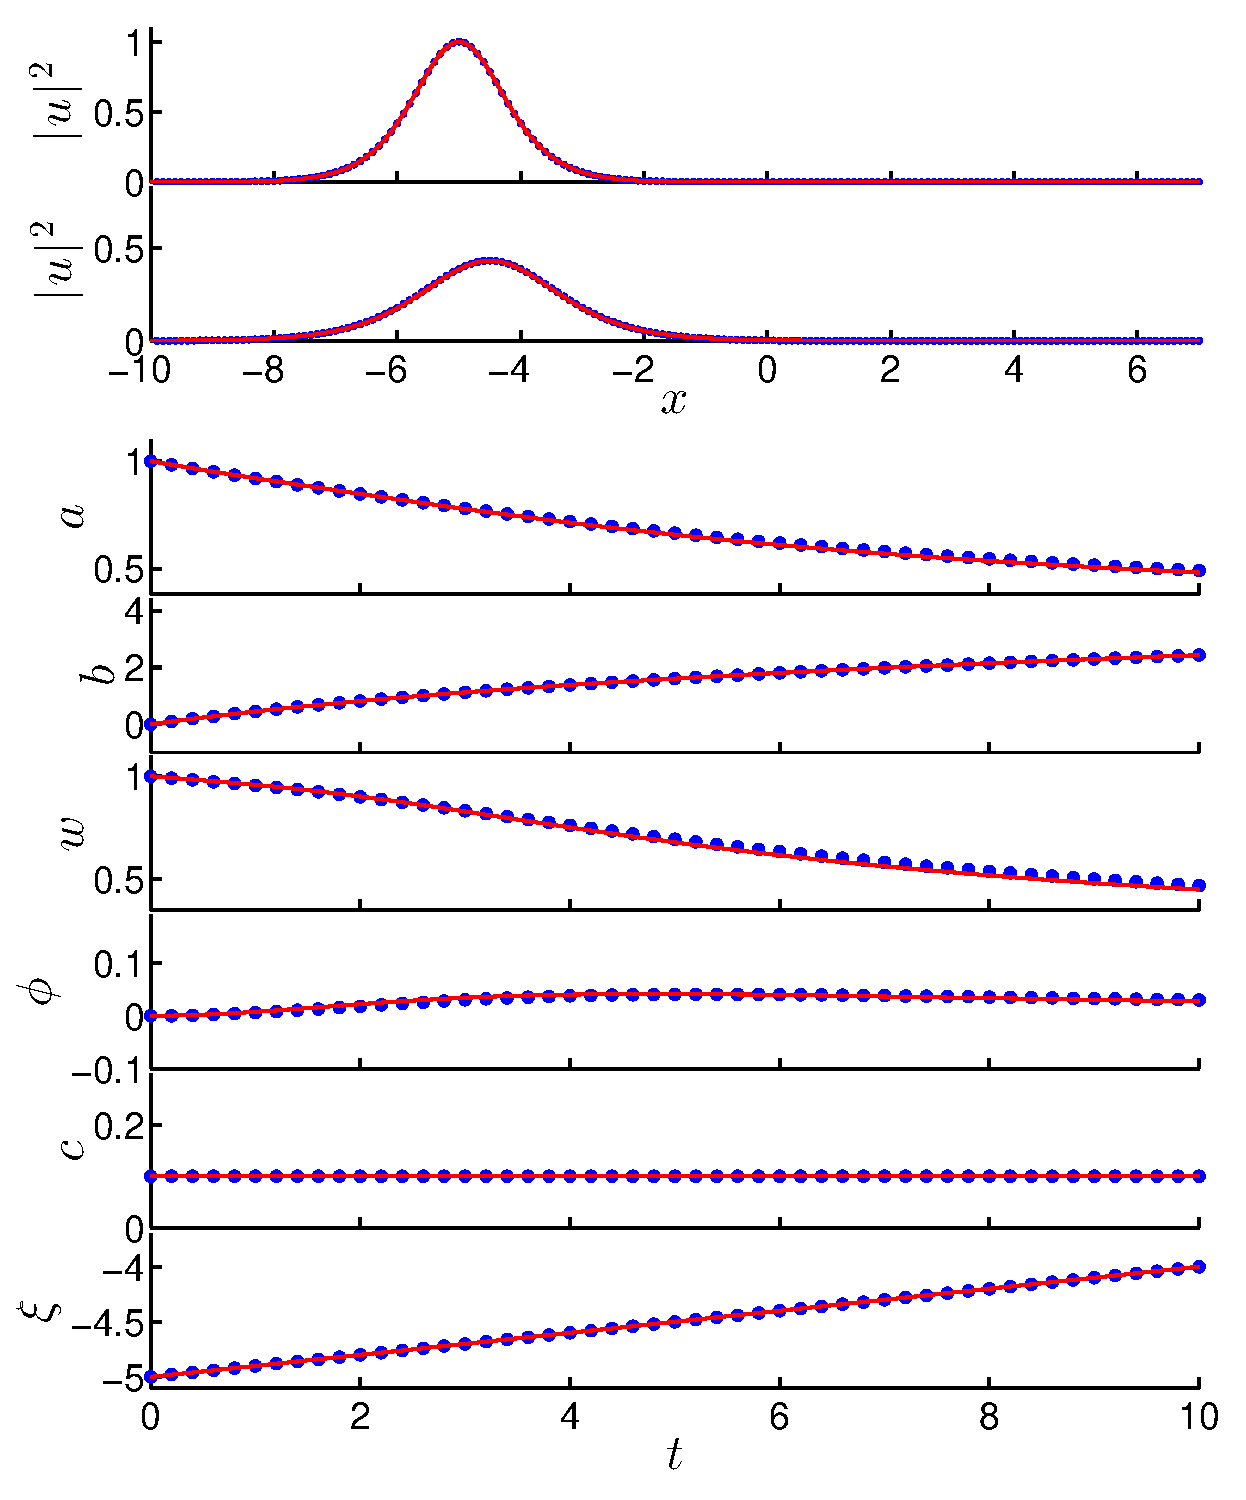
\includegraphics[width=0.8\textwidth]{Fig2_DD_e01N.eps}}
  \rule{35em}{0.5pt}
  \caption[NLS with Density Dependent Loss, $\epsilon = 0.1$]{Evolution of an NLS bright soliton under the presence of nonlinear loss of strength $\epsilon=0.1$.  The NCVA results are obtained from Eq.~(\ref{eq:NVCADD}) (red lines) while the full numerical solution is obtained from Eq.~(\ref{eq:NLSDD}) (blue dots).  Same initial conditions and layout of panels as in previous figures.}
   \label{fig:DDloss01}
\end{figure}
 
%\begin{figure}[htbp]
% \centering
%  \centerline{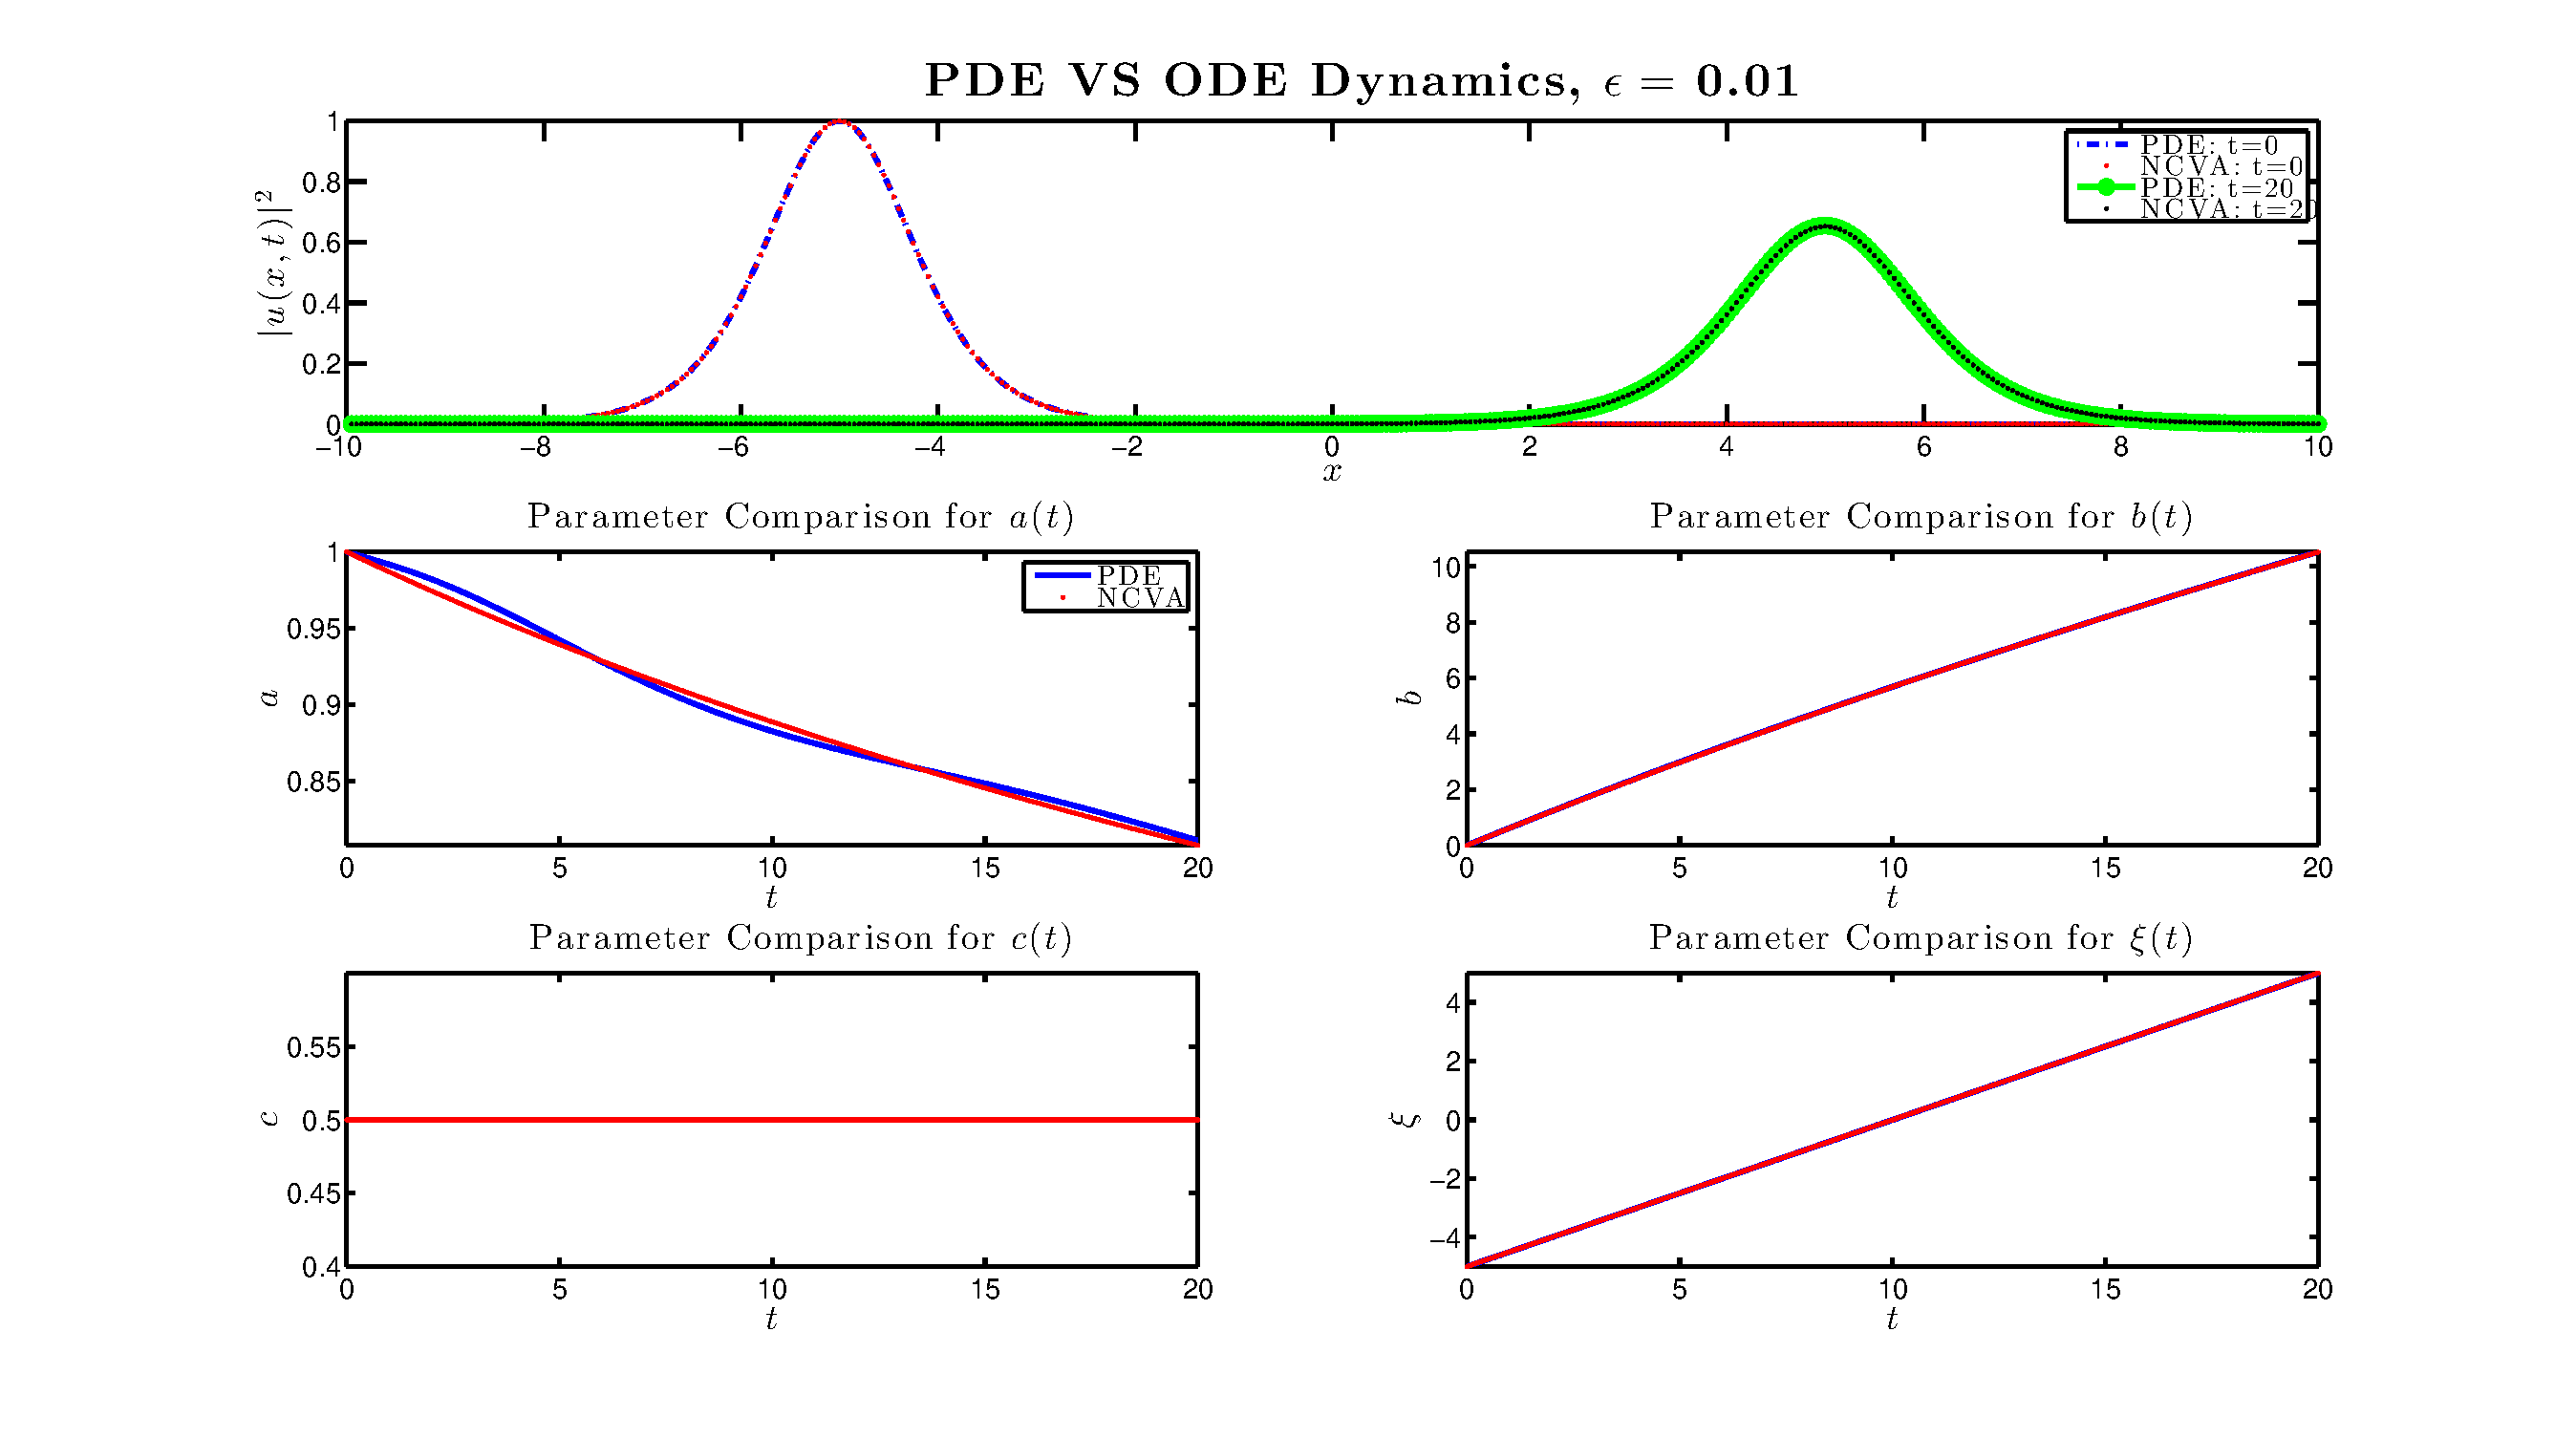
\includegraphics[width=1.2\textwidth, height=\textwidth]{DD001.eps}}
%  \rule{35em}{0.5pt}
%  \caption[NLS with Density Dependent Loss, $\epsilon = 0.01$]{{\bf NLS with Density Dependent Loss:} Comparison of ODE dynamics for the parameters $a$, $b$, $c$, and $\xi$ between forward integration of the PDE and the NCVA for $\epsilon=0.01$.}
%   \label{fig:DDloss001}
%\end{figure}
%
%
%\begin{figure}[htbp]
%  \centering
%  \centerline{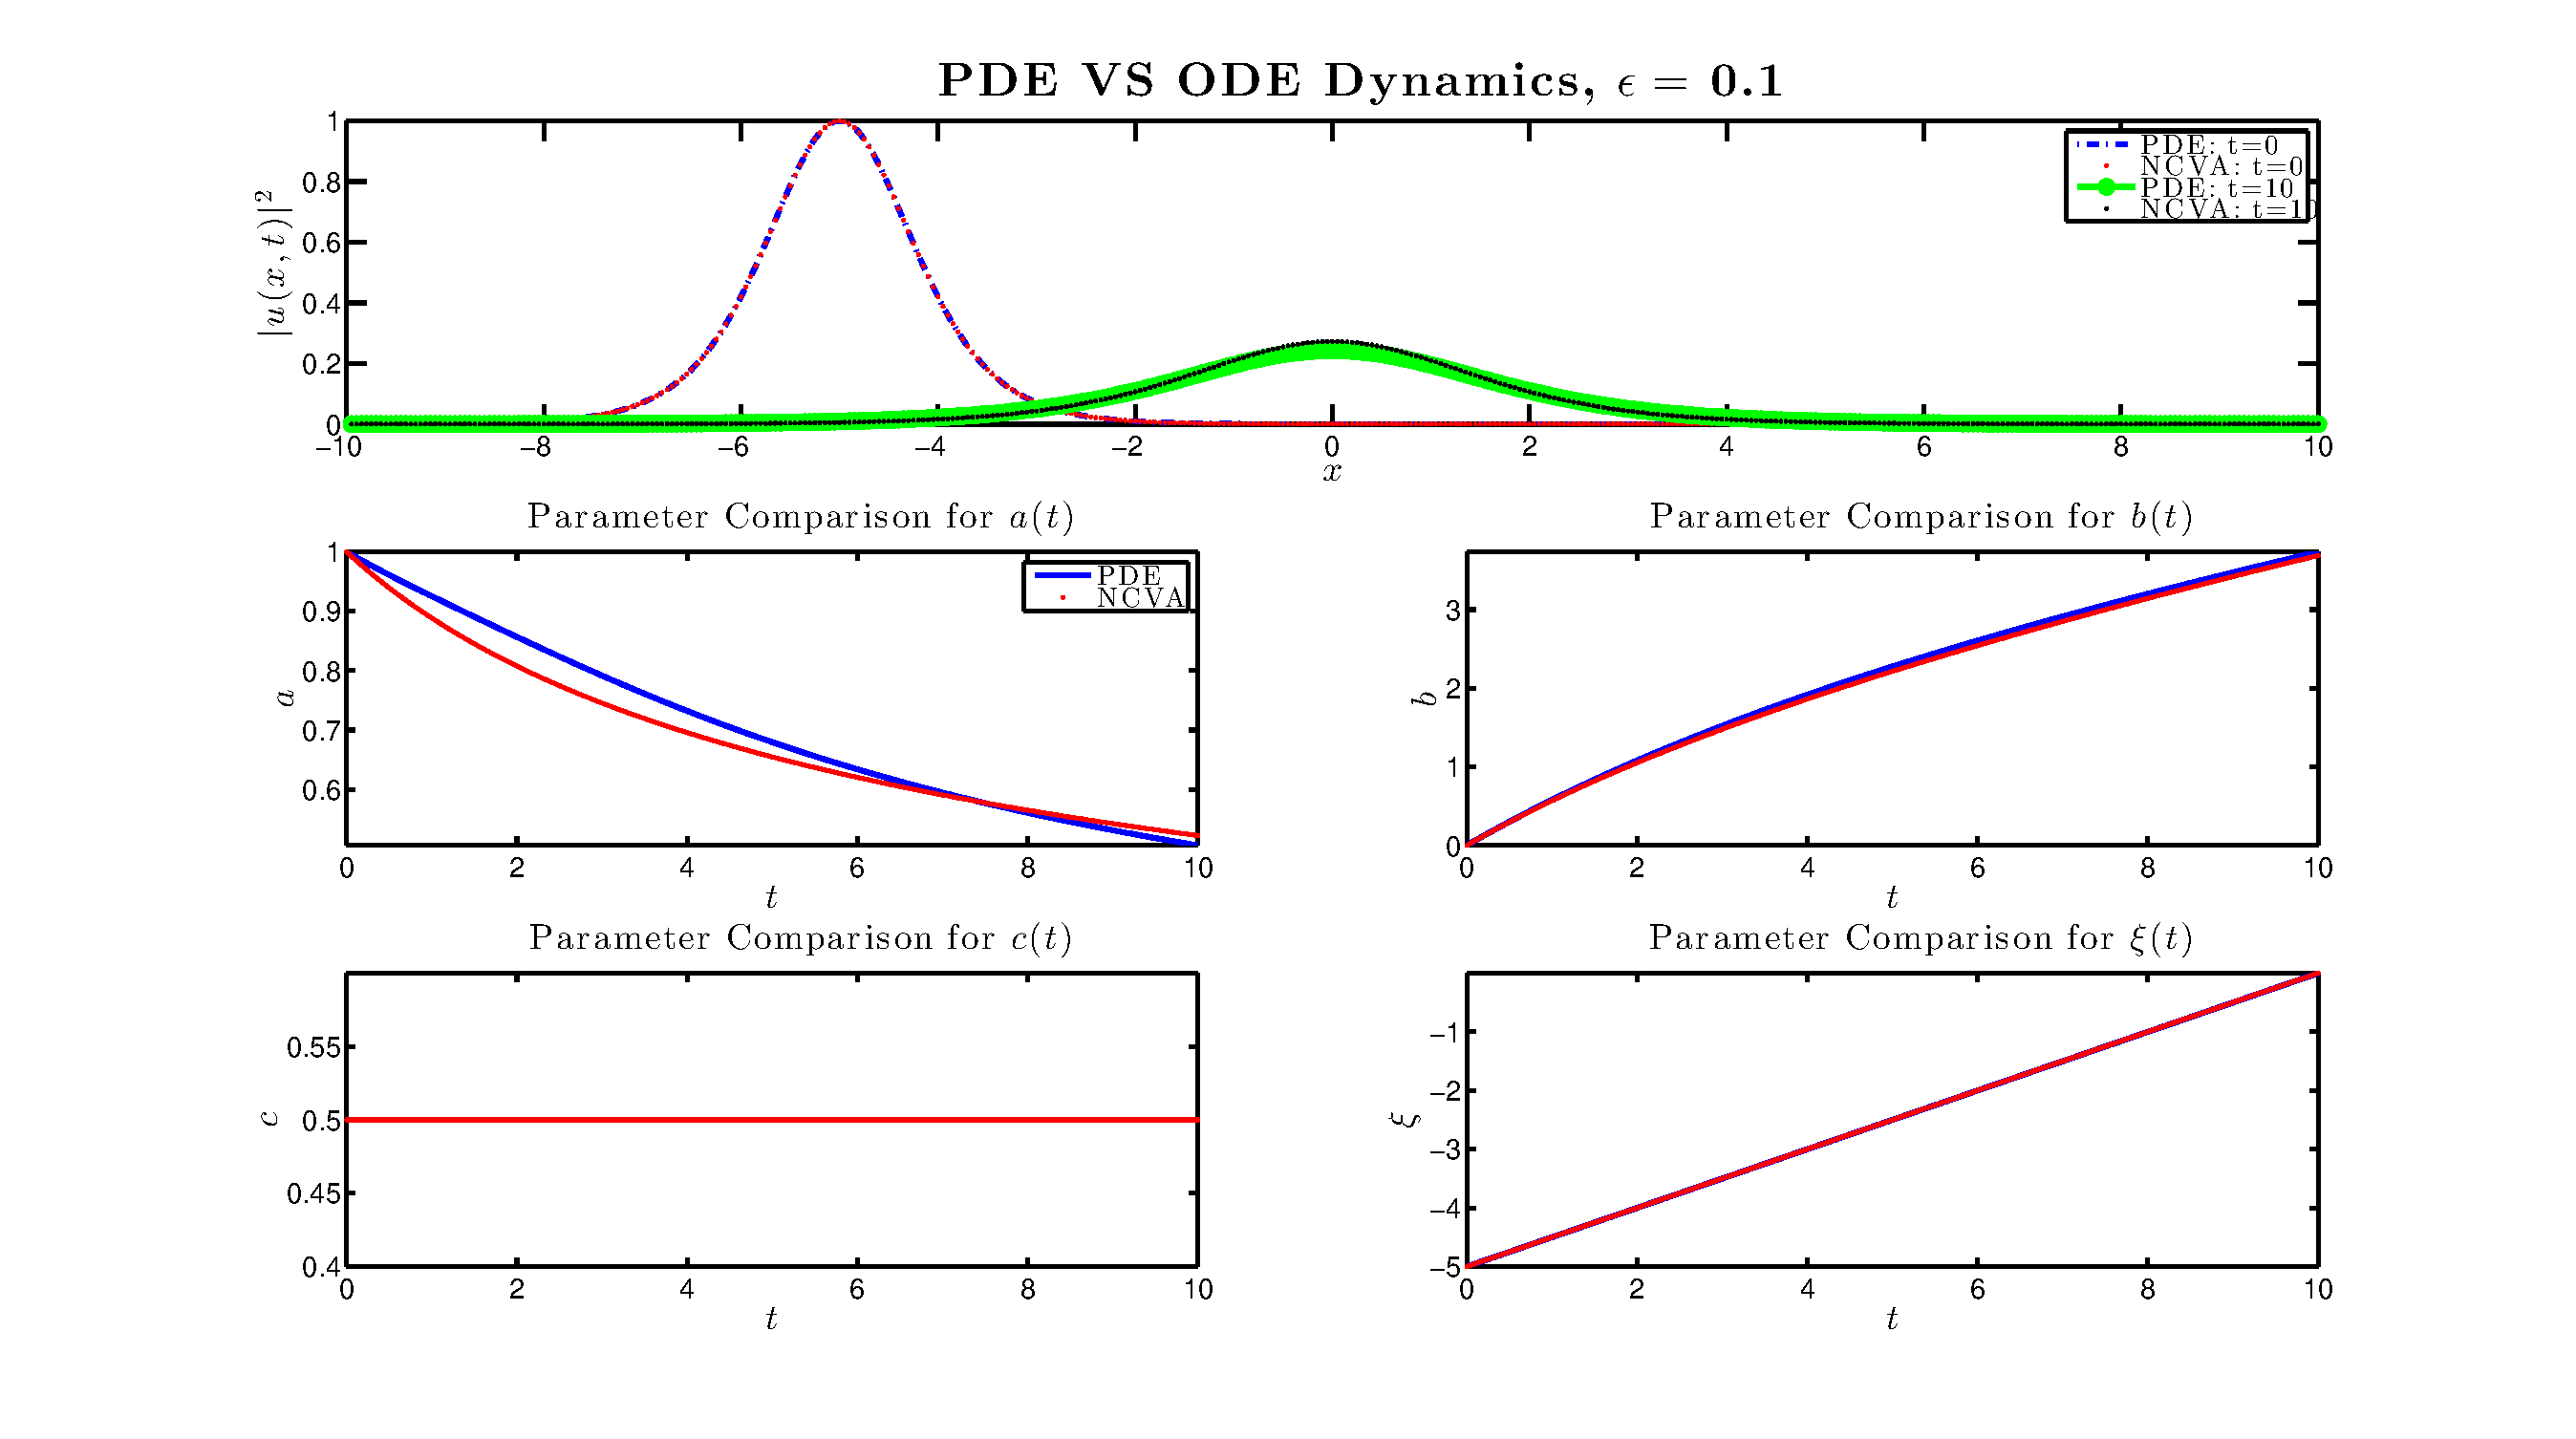
\includegraphics[width=1.2\textwidth, height=\textwidth]{DD01.eps}}
%  \rule{35em}{0.5pt}
%  \caption[NLS with Density Dependent Loss, $\epsilon = 0.1$]{{\bf NLS with Density Dependent Loss:} Comparison of ODE dynamics for the parameters $a$, $b$, $c$, and $\xi$ between forward integration of the PDE and the NCVA for $\epsilon=0.1$.}
%   \label{fig:DDloss01}
%\end{figure}
%
%
%\begin{figure}[htbp]
%\centering
%\begin{subfigure}[t]{0.49\textwidth}
%  		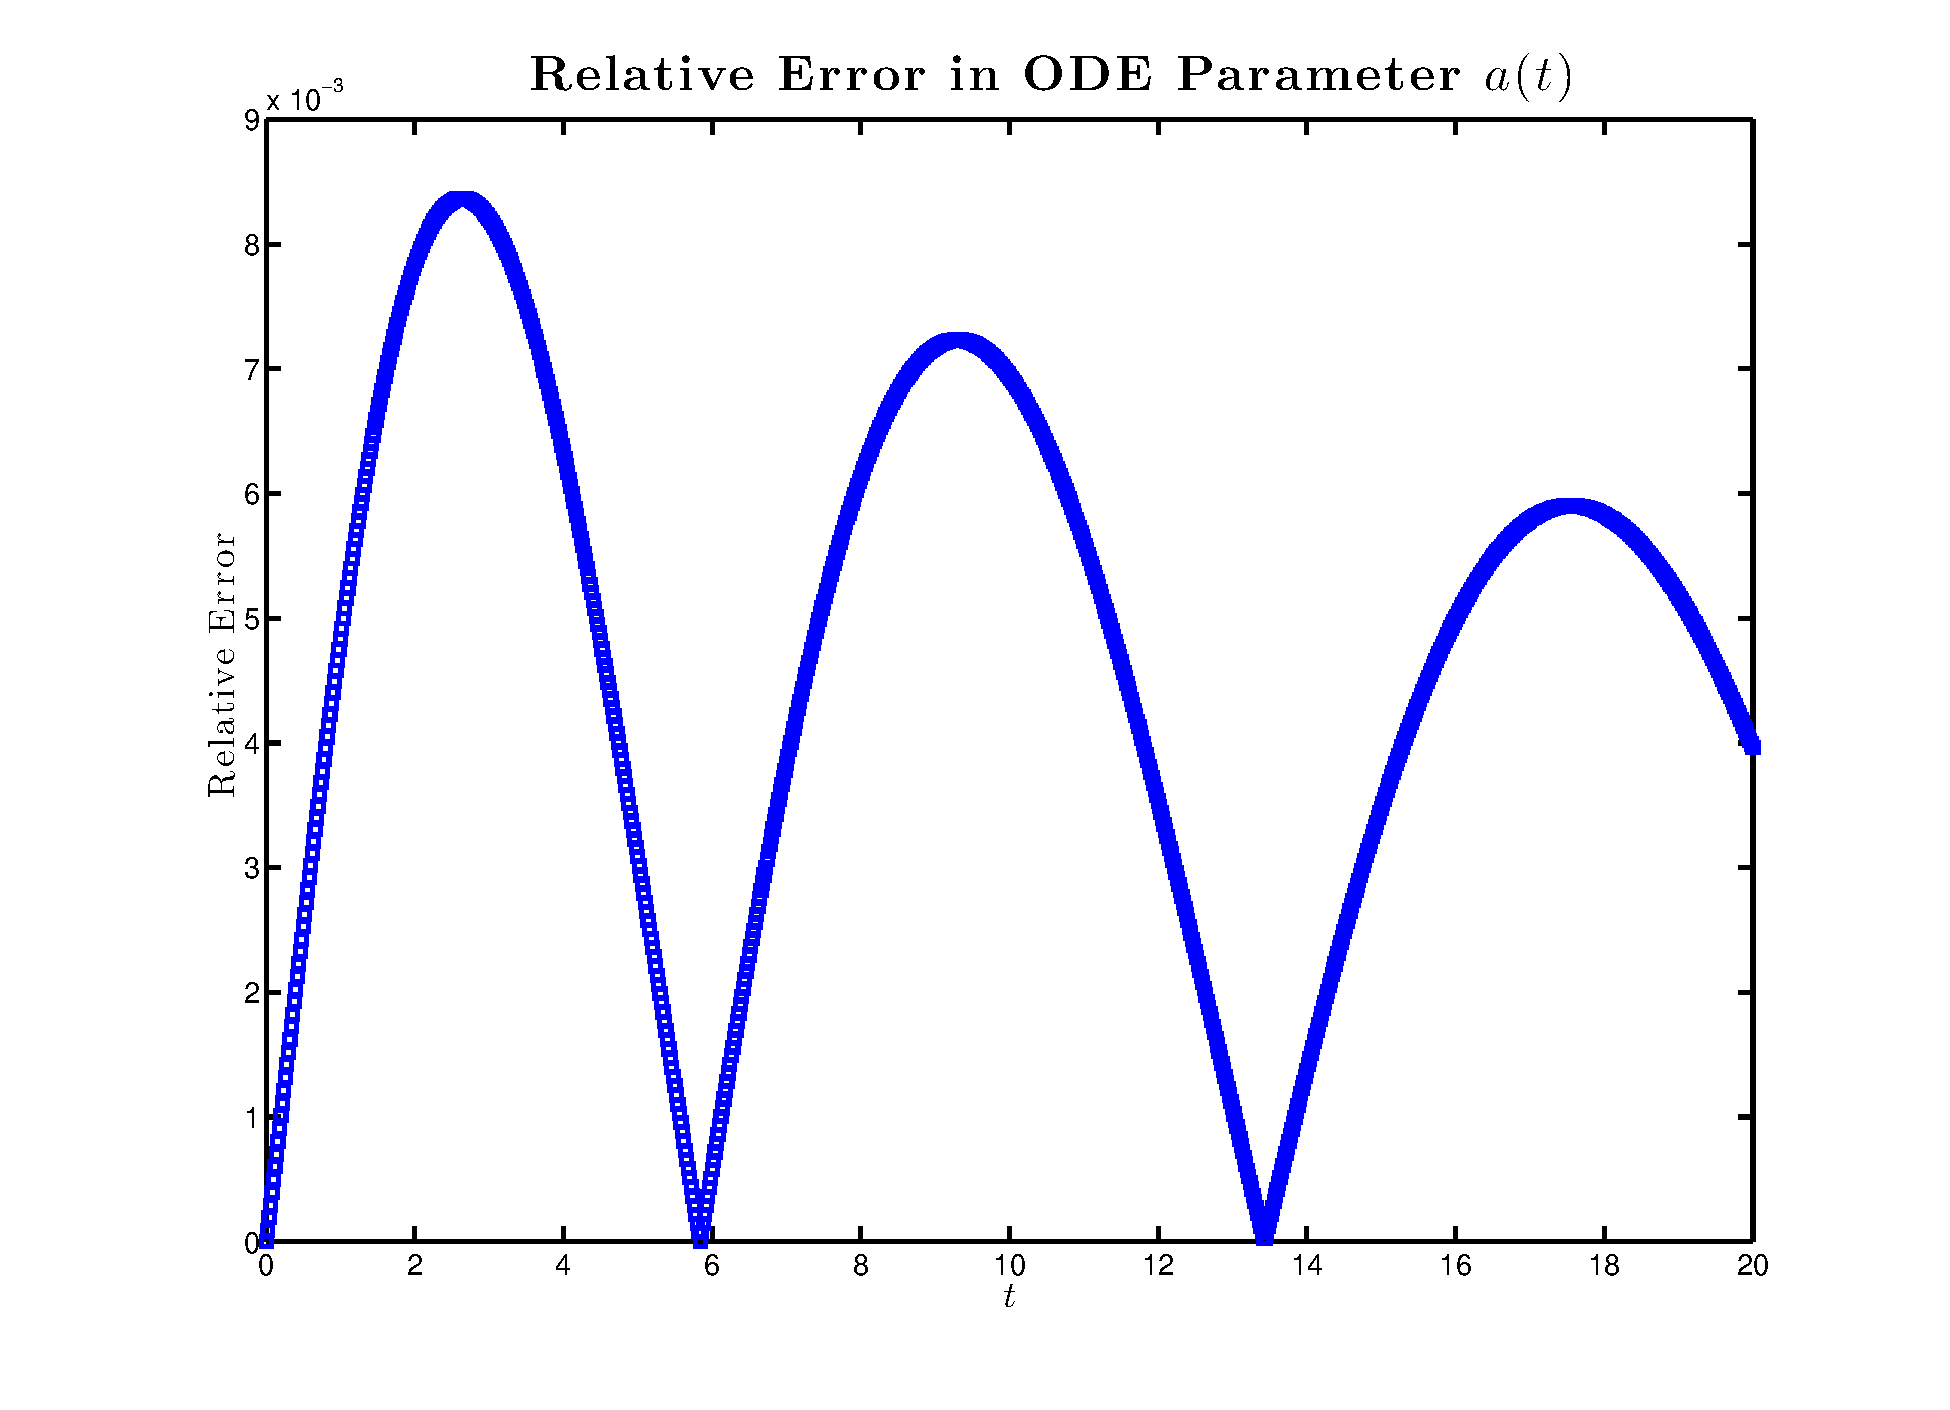
\includegraphics[width=\textwidth, height = \textwidth]{DD001relativeerror.eps}
%	         \caption{Relative error between NCVA and PDE parameter $a(t)$ values for $\epsilon=0.01$.}
%	         \label{fig:DLoss001Err}
%	     \end{subfigure}
%  \begin{subfigure}[t]{0.49\textwidth}
%  		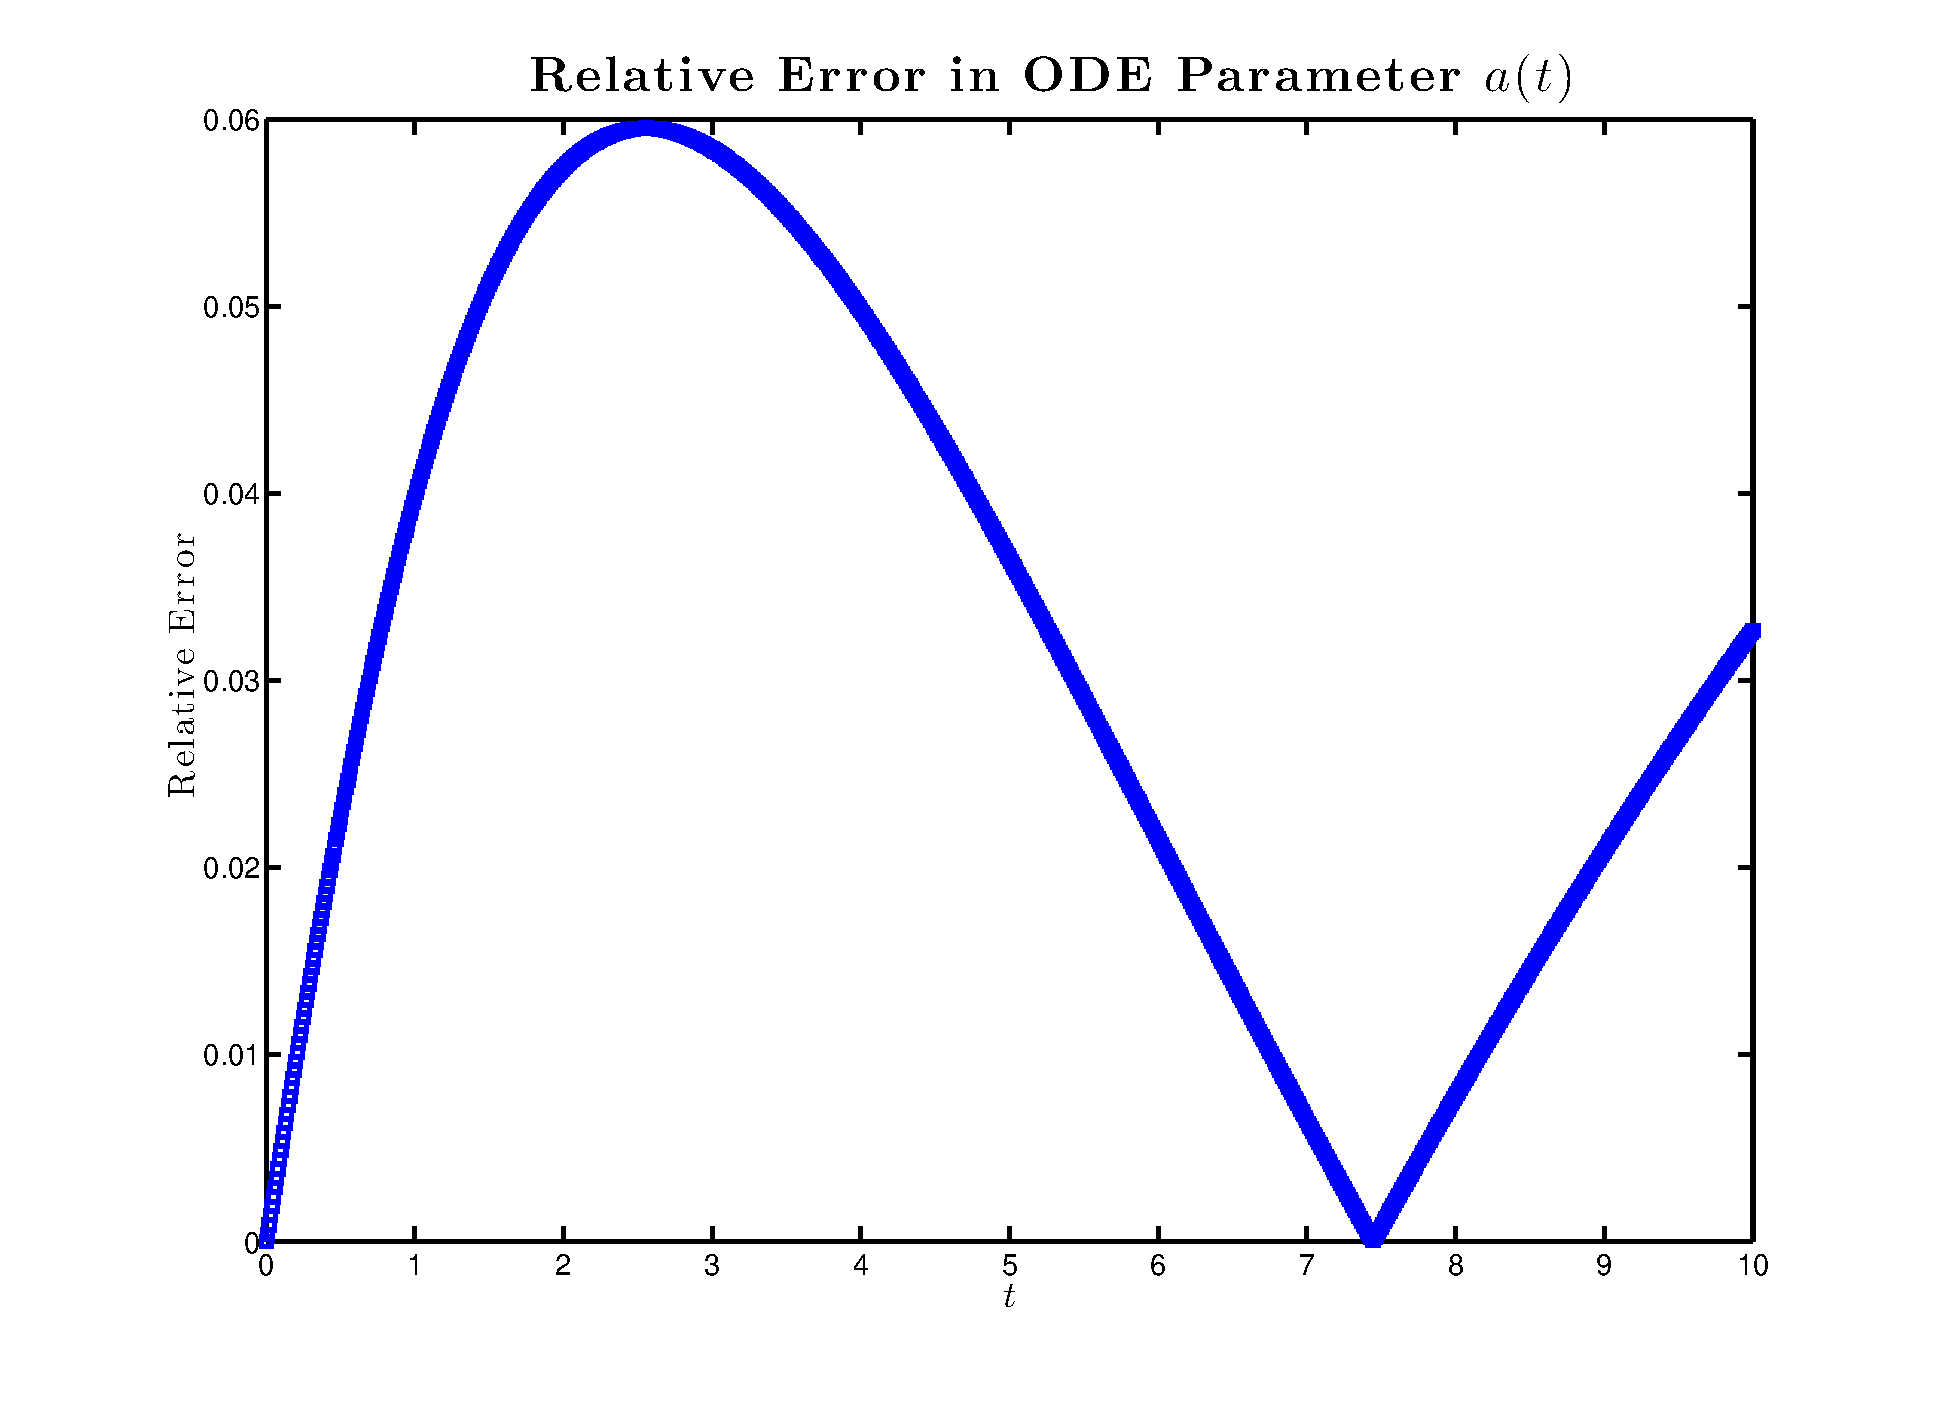
\includegraphics[width= \textwidth, height = \textwidth]{DD01relativeerror.eps}  
%	          \caption{Relative error between NCVA and PDE parameter $a(t)$ values for $\epsilon=0.1$.}
%	         \label{fig:DLoss01Err}
%	    \end{subfigure} 
%  \rule{35em}{0.5pt}
%   \caption[Relative Error in Amplitude for NLS with Density Dependent Loss]{{\bf NLS with Density Dependent Loss:} Amplitude parameter $a(t)$ relative error for (A) $\epsilon=0.01$ and (B) $\epsilon=0.1$.}
%   \label{fig:LLossA}
%\end{figure}

%\begin{figure}[htbp]
%\centering
%\begin{subfigure}[t]{0.49\textwidth}
%  		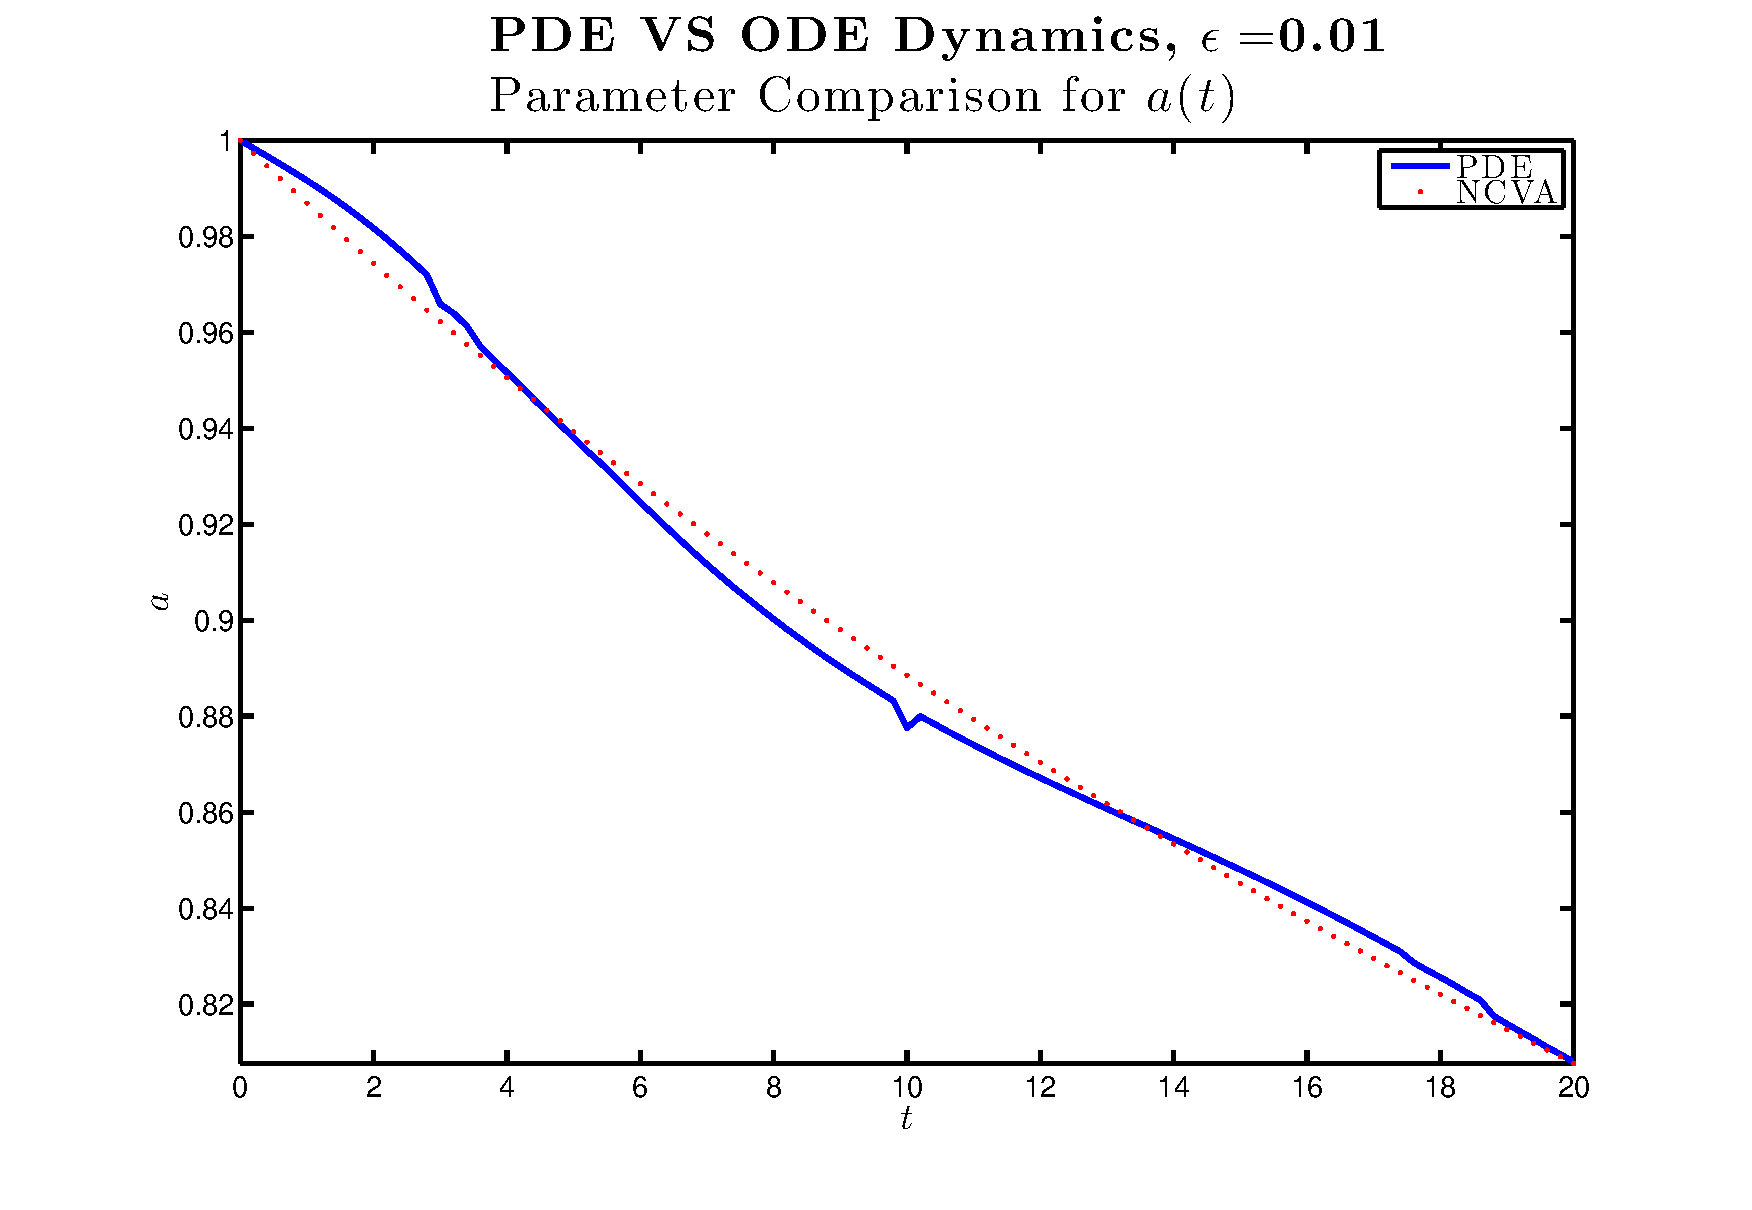
\includegraphics[width=\textwidth, height = \textwidth]{DDE001a.eps}
%	         \caption{Amplitude parameter comparison $a(t)$ between PDE and NCVA solutions.}
%	         \label{fig:DLoss001a}
%	     \end{subfigure}
%  \begin{subfigure}[t]{0.49\textwidth}
%  		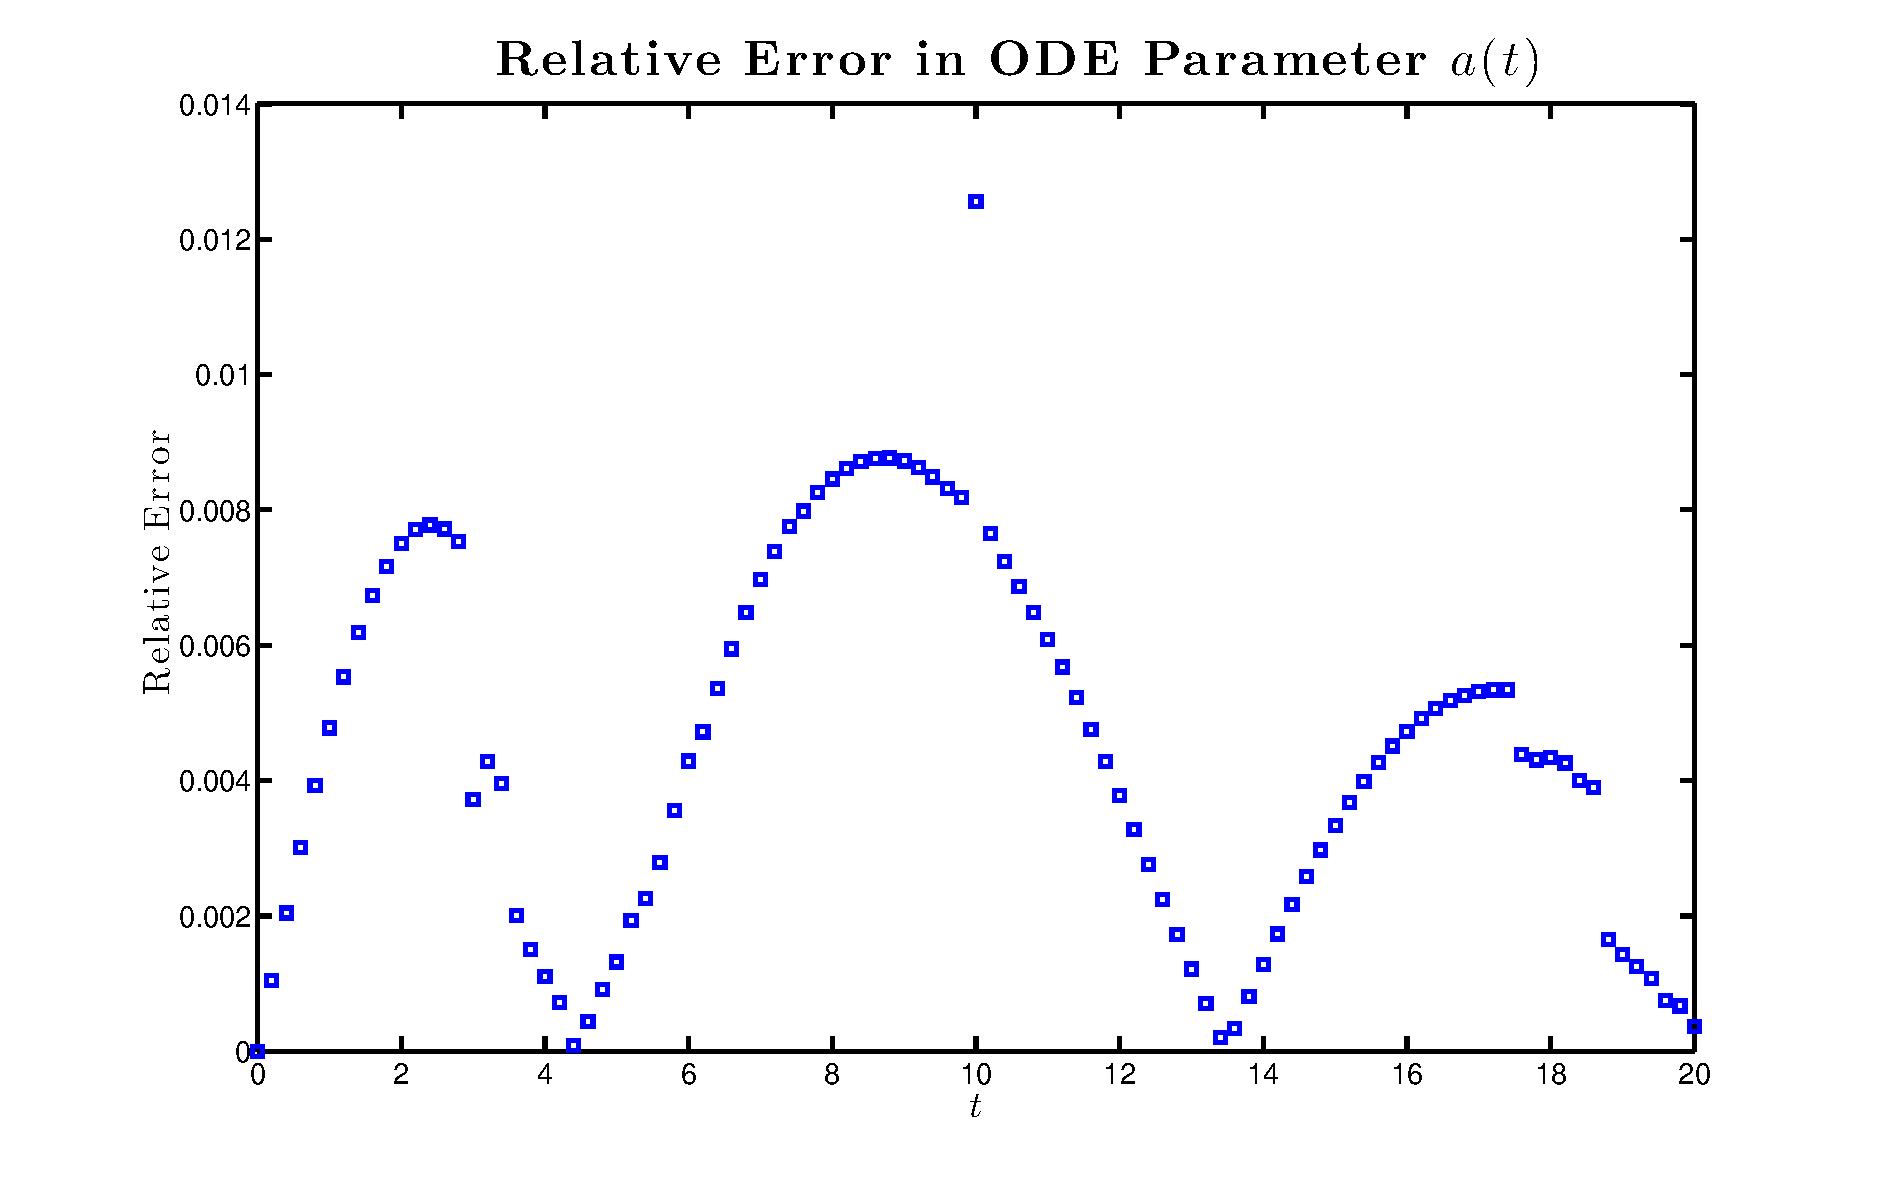
\includegraphics[width= \textwidth, height = \textwidth]{DDE001relativeError.eps}  
%	          \caption{Relative error between NCVA and PDE parameter $a(t)$ values.}
%	         \label{fig:DLoss001Err}
%	    \end{subfigure} 
%  \rule{35em}{0.5pt}
%   \caption[NLS with Density Dependent Loss, $\epsilon = 0.01$ Amplitude Comparison and Relative Error]{{\bf NLS with Density Dependent Loss:} Amplitude parameter $a(t)$ ansatz comparisons and relative error for $\epsilon=0.01$.}
%   \label{fig:DDlossA}
%\end{figure}
%
%
%\begin{figure}[htbp]
%\begin{subfigure}[b]{0.5\textwidth}
%  		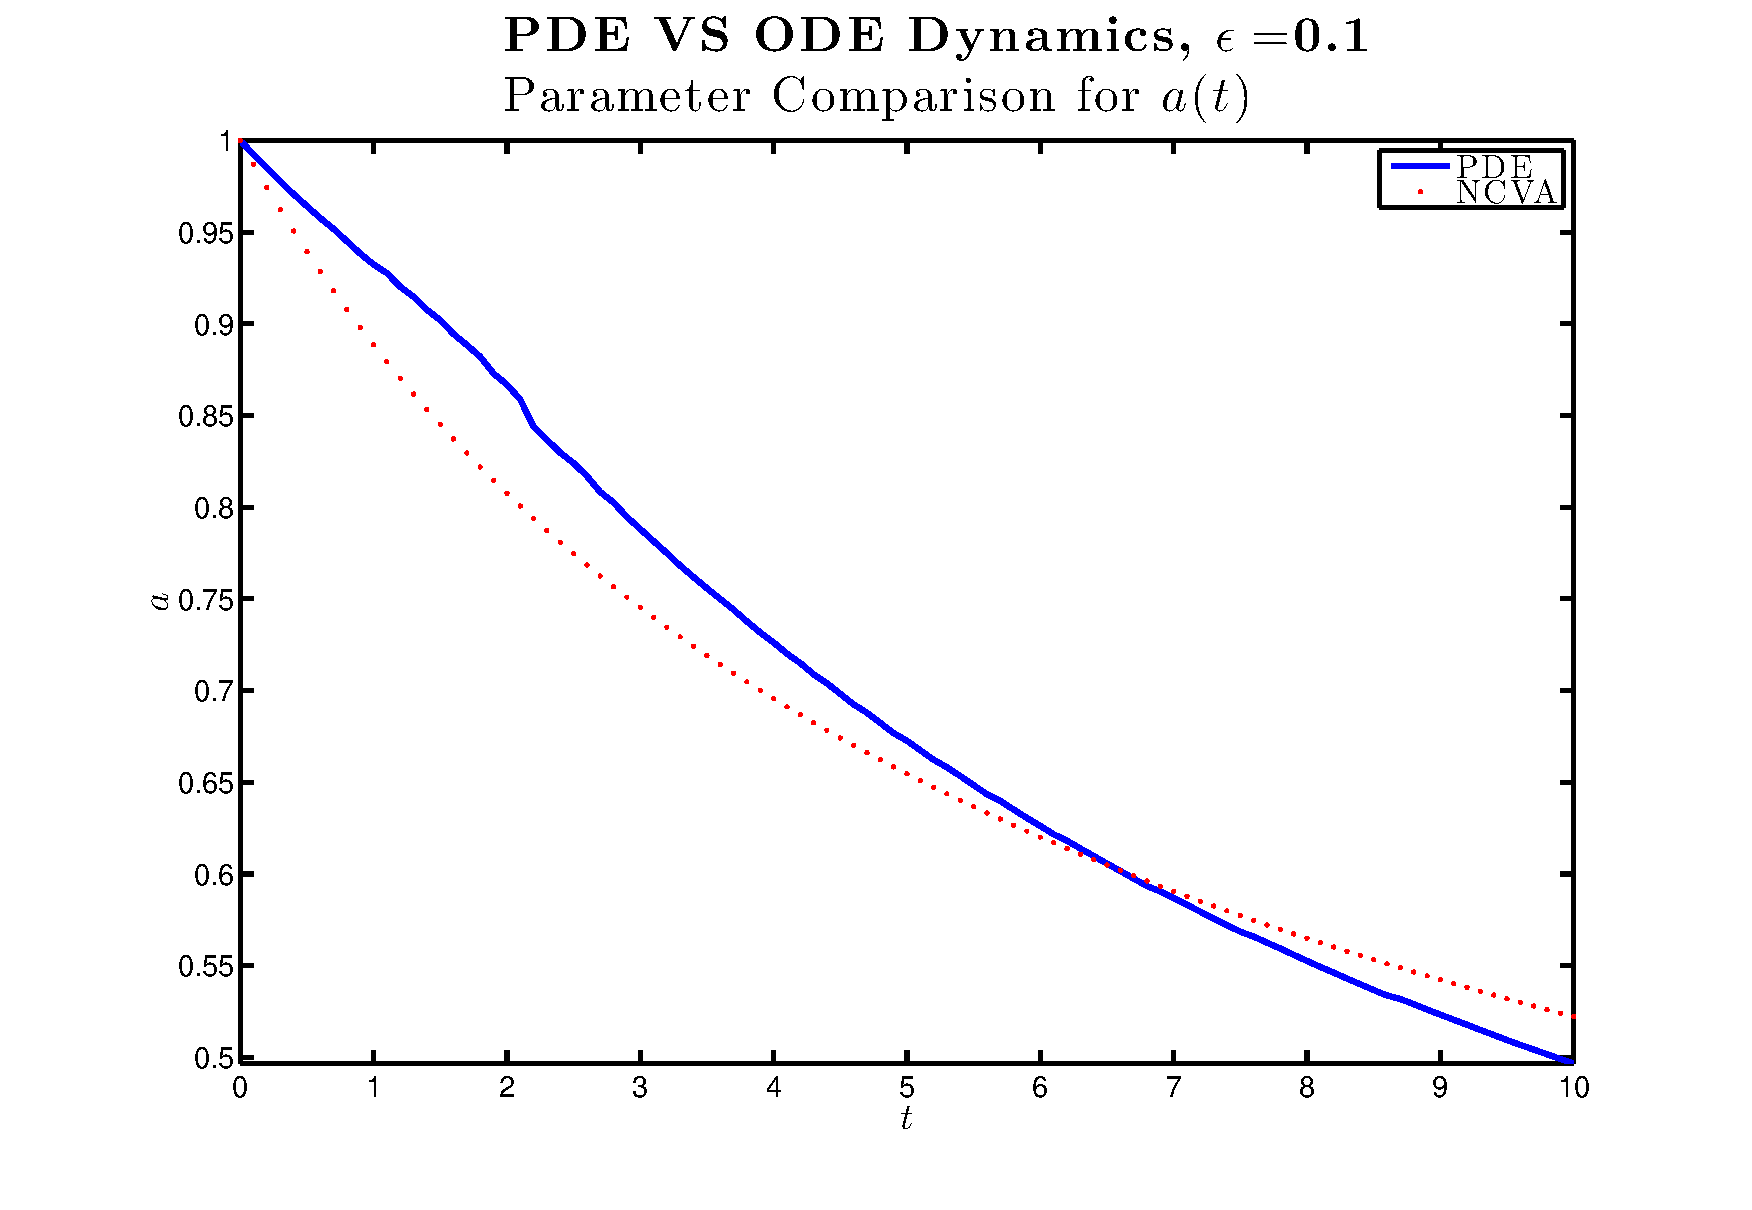
\includegraphics[width=\textwidth, height = \textwidth]{DDE01a.eps}
%	         \caption{Amplitude parameter comparison $a(t)$ between PDE and NCVA solutions.}
%	         \label{fig:DLoss01a}
%	     \end{subfigure}
%  \begin{subfigure}[b]{0.5\textwidth}
%  		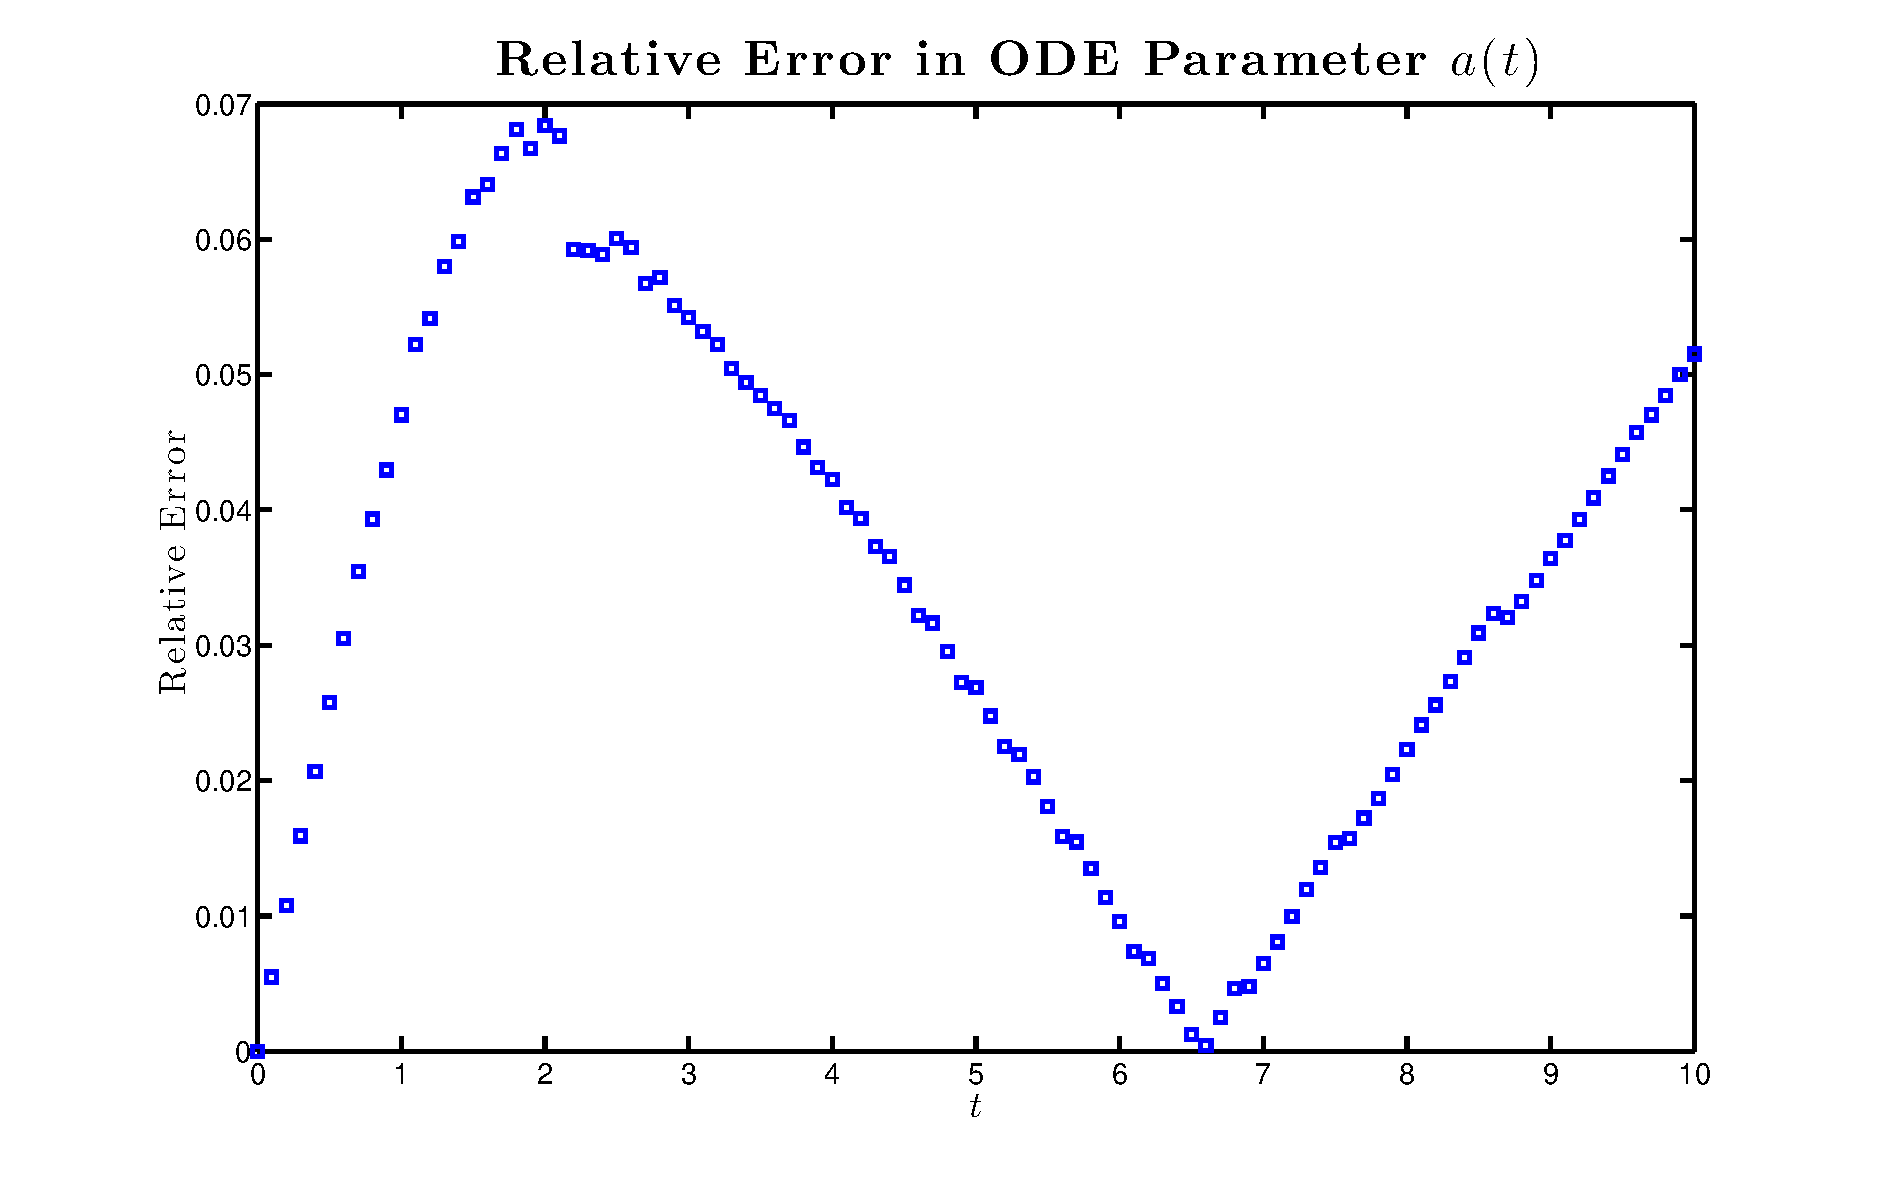
\includegraphics[width= \textwidth, height = \textwidth]{DDE01relativeError.eps}  
%	          \caption{Relative error between NCVA and PDE parameter $a(t)$ values.}
%	         \label{fig:DLoss01Err}
%	    \end{subfigure} 
%  \rule{35em}{0.5pt}
%   \caption[NLS with Density Dependent Loss, $\epsilon = 0.1$ Amplitude Comparison and Relative Error]{{\bf NLS with Density Dependent Loss:} Amplitude parameter $a(t)$ ansatz comparisons and relative error for $\epsilon=0.1$.}
%   \label{fig:DDlossA2}
%\end{figure}

\clearpage

%%%% Section Polariton - NLS with Linear Gain and Density Dependent loss %%%%%%%%%%%
{\setstretch{1.3}
\section[Exciton-Polariton Condensate - The Nonlinear Schr\"{o}dinger Equation with Linear Gain and Density Dependent Loss]{Exciton-Polariton Condensate -  NLS with Linear Gain and Density Dependent Loss}\label{section:EPCond}}

\setstretch{2}
The third dynamical system is based on exciton-polariton condensates.  
In exciton-polariton condensates, the condensing ``entities'' are excitons, namely
bound electron-hole pairs.  These excitons strongly couple with light when confined in quantum wells placed in
high-finesse microcavities, forming exciton-photon mixed quasi-particles known
as polaritons \cite{RMP}.  These condensates exist at finite temperatures, even near room temperature, which means the the polaritons can only exist for a few picoseconds in the cavity before they decay into photons.  The finite lifetime of the polaritons precludes the system from reaching thermal equilibrium, in fact, the system is a genuinely far-from-equilibrium condensate which requires an external pump from a reservoir of excitons to counter the loss of polaritons.

Exciton-polariton condensates offer numerous key features of the superfluid 
character including: the flow without scattering (analog of the flow without friction) \cite{amo1},
the existence of vortices \cite{lagou1}
and their interactions \cite{roumpos,roumpos2},
the collective superfluid dynamics \cite{amo2},
as well as remarkable applications such as spin switches \cite{amo3},
and light emitting diodes \cite{amo4} operating even near room temperatures.

There is a wide variety of different types of models for polaritons to describe the associate pumping and damping mechanisms.  One of these models,
proposed in Refs.~\cite{Keeling2008,kbb,berl_review},
suggests the use of a {\em single} NLS-type equation for the polariton
condensate wavefunction which incorporates a gain-loss mechanism for the decay of polaritons to photons and pumping of excitons from an external reservoir.  Specifically, this model, based on a repulsive ($g=-1$)
NLS equation with linear gain ($i\chi(x) u$)
and density dependent loss ($-i\sigma |u|^2 u$) terms, can be written
in the following non-dimensional form~\cite{ref8,Keeling2008}:
%
\begin{equation}
iu_t + \frac{1}{2} u_{xx} - |u|^2 u - V(x)u =  i\left[\chi(x) - \sigma  |u|^2\right] u, \label{eq:NLSP}
\end{equation}
where $\sigma$ is the strength of the density dependent loss and $\chi$ is considered the localized, spatially dependent gain given by 
\begin{equation}
\chi(x) = \alpha\exp\left(-\frac{x^2}{2 \beta^2}\right),
\label{eq:gainP}
\end{equation}
describing a laser pump of amplitude $\alpha$ and width $\beta$.  The potential $V$ is a general harmonic potential of strength $\Omega$:
\begin{equation}
V(x) = \frac{1}{2} \Omega^2 x^2.
\label{eq:potP}
\end{equation}
For the application of variational approximations, we define the Gaussian ansatz 
\begin{equation}
u_A (x,t; \vec{p}) = a e^{ -\frac{x^2}{2w^2}}  e^{i\left(b x^2 + \phi\right)}, \label{eq:GaussAnsatz}
\end{equation}
where the ansatz parameter $\vec{p}_i = (a_i, w_i, b_i, \phi_i)$ for $i=1$ and 2
represent, respectively, the amplitude, width, chirp, and phase of the ansatz solution.  The departure from a ${\rm sech}$-type ansatz is based on two reasons: (i) the Hamiltonian NLS has a Gaussian-type solution for a low density condensate, and (ii) given a Gaussian-type gain, this ansatz allows us to obtain explicit ODEs through the NCVA.
%
%described by a generic NLS equation with linear gain ($i\chi u$) and density dependent loss ($-i\sigma |u|^2 u$) terms~\cite{Cuevas2011, Keeling2008}:
%\begin{align}
%iu_t + \frac{1}{2} u_{xx} + |u|^2 u =  i(\chi - \sigma  |u|^2) u,
%\end{align}
%where $\chi$ and $\sigma$ are, respectively, the gain and loss coefficients. 
%The Lagrangian corresponding to the conservative portion ($\chi = 0$ and $\sigma=0$) is given by:
%\begin{align}
%L = \frac{i}{2} \Bigg( u \frac{\partial u^*}{\partial t} -u^* \frac{\partial u}{\partial t} \Bigg) + \frac{1}{2} \Bigg| \frac{\partial u}{\partial x} \Bigg|^2  - \frac{1}{2} | u|^4.
%\end{align}
%The proposed ansatz is
%\begin{align}
%u(x,t) = a \mathrm{sech}(a(x-\xi))e^{i(c(x-\xi)+b)}
%\end{align}
%with function parameters $a$, $b$, $c$, and $\xi$. 

%\subsection{Perturbed Variational Approximation}
%In the perturbed and Kantorovitch variational approximation methods, the non-conservative terms are 
%\begin{align}
%\mathcal{P} = \chi \mathcal{Q}_{\mathrm{gain}} + \sigma \mathcal{Q}_{\mathrm{loss}} = i(\chi - \sigma  |u|^2) u,
%\end{align}
%such that $\mathcal{Q}_{\mathrm{gain}} = i u$ and $\mathcal{Q}_{\mathrm{loss}} = - i |u|^2 u$
%%According to Cerda's~\cite{Cerda} method the non-conservative terms are described as
%%\begin{align}
%%Q = i(\chi - \sigma  |u|^2) u,
%%\end{align}
%and the two solutions are equivalent.  From the modified Kantorovitch method and the perturbed variational approximation it is straightforward to obtain a system of four coupled ODEs for the exciton-polariton condensate:
%%\begin{align} \begin{cases}
%%2 \dot{b} - a^2 - 2c\dot{\xi} + c^2 = 0, \\
%%-2\dot{a} = -4\chi a +  \frac{8}{3} \sigma a^3, \\
%%-2\dot{\xi} a + 2ac = 0, \\
%%2 \dot{a} c + 2 a \dot{c} = 4\chi a c -\frac{8}{3} \sigma a^3 c. 
%%\end{cases} \end{align} 
%%The four equations are solved simultaneously to find the following system of ODEs for the exciton-polariton condensate: 
% \begin{equation}
% \begin{cases}
%  \dot{a} = \frac{\sqrt{2}}{8} \sigma a^3 -\frac{3\sqrt{2}}{4} \frac{\sigma a^3 w^2}{w^2 + 2\beta^2 } + \frac{3\sqrt{2}}{2} \frac{\alpha \beta a w^2}{\left( w^2 + 2 \beta^2 \right)^{3/2}} -\frac{3\sqrt{2}}{2} \frac{\sigma \beta^2 a^3 }{w^2 + 2\beta^2} + \frac{2\sqrt{2} \alpha \beta^3 a}{\left( w^2 + 2\beta^2\right)^{3/2}} - ab , \\
%\dot{b}  = \frac{\sqrt{2}}{4} \frac{a^2}{w^2} + \frac{1}{2 w^4} - \frac{1}{2} \Omega^2 - 2b^2, \\
%\dot{w} = -\frac{5\sqrt{2}}{4} \sigma a^2 w + \frac{3\sqrt{2}}{2} \frac{\sigma a^2 w^3}{w^2 + 2\beta^2} - \frac{\sqrt{2} \alpha \beta w^3}{\left( w^2 + 2\beta^2 \right)^{3/2}} +\frac{3\sqrt{2} \sigma \beta^2 a^2 w }{w^2 + 2\beta^2} + 2 w b, \\
%\dot{\phi} = -\frac{5\sqrt{2}}{8} a^2 -\frac{1}{2w^2} .
%\end{cases}
% \label{eq:PVAP}
% \end{equation}
%%\begin{align}\begin{cases}
%%\dot{a} = 2\chi a -\frac{4}{3} \sigma a^3, \\
%%\dot{b} = \frac{1}{2} a^2 + \frac{1}{2} c^2, \\
%%\dot{c} = 0,\\
%%\dot{\xi} = c.
%%\end{cases} \label{eq:PVAP}\end{align}

\subsection{Non-conservative Variational Approximation}
In the NCVA, we use two ans\"atze $\bar{u}_1= u_A(x,t; \vec{p_1})$ and $\bar{u}_2=u_A(x,t; \vec{p_2})$ as defined by the Gaussian profile of Eq.~(\ref{eq:GaussAnsatz}).  The selection of a Gaussian profile is to characterize the breathing motion of a ground state inside the trap, rather than to characterize the translational dynamics of the wavefunction.  In order to find translational modes, we would require a different ansatz with an added degree of freedom corresponding to a center position parameter of the wavefunction.

According to the NCVA method, the Lagrangian is $\bar{\mathcal{L}} = \bar{\mathcal{L}}_1 - \bar{\mathcal{L}}_2 +\bar{\mathcal{R}}$, where the conservative terms have the Lagrangian densities for $i= 1,$ 2 given by 
\begin{eqnarray}
\bar{\mathcal{L}_i} &= \frac{i}{2} \left(\bar{u}_i \bar{u}_{i,t}^* - 
\bar{u}_i^* \bar{u}_{i,t}\right) + \frac{1}{2} |\bar{u}_{i,x}|^2 + \frac{1}{2}|\bar{u}_i|^4 + V(x) |\bar{u}_i|^2,
%\bar{\mathcal{L}_1} &= \frac{i}{2} \left(\bar{u}_1 \bar{u}_{1,t}^* - 
%\bar{u}_1^* \bar{u}_{1,t}\right) + \frac{1}{2} |\bar{u}_{1,x}|^2 + \frac{1}{2}|\bar{u}_1|^4 + V(x) |\bar{u}_1|^2,  \\
%\bar{\mathcal{L}}_2 &= \frac{i}{2} \left(\bar{u}_2 \bar{u}_{2,t}^* - \bar{u}_2^* \bar{u}_{2,t}\right) + \frac{1}{2} |\bar{u}_{2,x}|^2 + \frac{1}{2}|
%\bar{u}_2|^4 + V(x) |\bar{u}_2|^2, %\quad\\[1.0ex]
\end{eqnarray}
and $\bar{\mathcal{R}}$ has the same type of density dependent loss [see Section~\ref{section:DD}] and a linear gain (equivalent to the negative of linear loss)  [see Section~\ref{section:NCVALL}] shown in the previous examples.  The non-conservative terms are defined as follows:
\begin{eqnarray}
\bar{\mathcal{R} }&=& \, \bar{\mathcal{P}} u_-^*+ \bar{\mathcal{P}}^*u_-,  \\
&=& -i \chi(x) \left( \bar{u}_2 \bar{u}_1^* -  \bar{u}_1  \bar{u}_2^* \right) \\ \nonumber
&& + i\sigma [ | \bar{u}_1|^2 \left(  \bar{u}_2  \bar{u}_1^* -  \bar{u}_2^*  
\bar{u}_1 \right) +  | \bar{u}_2|^2 \left(  \bar{u}_2  \bar{u}_1^*  - \bar{u}_2^*  \bar{u}_1 \right) +  \bar{u}_2  \bar{u}_2  \bar{u}_1^*  \bar{u}_1^* -  \bar{u}_1  
\bar{u}_1  \bar{u}_2^*  \bar{u}_2^2  ]. 
\end{eqnarray}
%
%In the non-conservative variational approximation $u_1$ and $u_2$ ansatz are defined as
%\begin{align}
%u_1 &= a_1 \mathrm{sech}(a_1(x-\xi_1))e^{i(c_1 (x-\xi_1)+b_1)}, \\
%u_2 &= a_2 \mathrm{sech}(a_2(x-\xi_2))e^{i(c_2 (x-\xi_2)+b_2)}.
%\end{align}
%According to the non-conservative variational method the Lagrangian is $\mathscr{L} = L_1 - L_2 + R$ where 
%\begin{align}
%L_1 =& \frac{i}{2} \Big(u_1 u_{1,t}^* - u_1^* u_{1,t}\Big) + \frac{1}{2} |u_{1,x}|^2 - \frac{1}{2}|u_1|^4, \\
%L_2 =& \frac{i}{2} \Big(u_2 u_{2,t}^* - u_2^* u_{2,t}\Big) + \frac{1}{2} |u_{2,x}|^2 - \frac{1}{2}|u_2|^4, \\
%Q =&  -i\chi u_+ u_-^* + i\sigma  u_+ u_+^* u_+u_-^* \nonumber \\
%=&  -i \chi \frac{(u_1 + u_2)}{2}(u_1 - u_2)^*  +  i \sigma  \frac{(u_1 + u_2)}{2}\frac{(u_1^* + u_2^*)}{2}\frac{(u_1 + u_2)}{2}(u_1 - u_2)^* \nonumber \\
%=& -\frac{i}{2} \chi (u_1u_1^* - u_2 u_2^* + u_2u_1^* - u_1 u_2^*) \nonumber \\
%&+ \frac{i}{8} \sigma (|u_1|^4 - |u_2|^4 + |u_1|^2(2u_2u_1^*) -  |u_2|^2(2u_1 u_2^*)  + u_2u_2 u_1^*u_1^* - u_1u_1u_2^*u_2^*) \\
%\begin{align}
%R =& \, Q + Q^*, \nonumber \\
%=& -i \chi (u_2u_1^* - u_1 u_2^* ) + i\sigma ( u_+ u_+^* u_+u_-^* -  u_+ u_+^* u_-u_+^*).
%\end{align}
%The modified Euler-Lagrange equations:
%\begin{align}
%\frac{\partial L}{\partial p} - \frac{d}{dt} \Bigg( \frac{\partial L }{\partial\dot{p}}\Bigg) + \int \Big[ \frac{\partial R}{\partial p_-} \Big]_{\mathrm{PL}} dx = 0. 
%\end{align}
%The total Lagrangian:
%\begin{align} \bar{L} =& 2\dot{b}_1a_1 - \frac{1}{3}a_1^3 + c_1^2 a_1 - 2c_1 \dot{\xi}_1a_1 - 2\dot{b}_2 a_2 + \frac{1}{3}a_2^3 - c_2^2 a_2 + 2c_2 \dot{\xi}_2 a_2  \nonumber  \\ 
%&- i \chi \int \Big[ \frac{\partial}{\partial p_-} \Big(u_2u_1^* - u_1u_2^*)\Big]_{\mathrm{PL}} dx \nonumber \\ 
%&+ \frac{i}{4} \sigma \int \Big[ \frac{\partial}{\partial p_-} \Big(|u_1|^2( u_2u_1^* - u_2^* u_1) +  |u_2|^2( u_2u_1^* - u_2^* u_1)  + u_2u_2 u_1^*u_1^* - u_1u_1u_2^*u_2^*\Big) \Big]_{\mathrm{PL}} dx . \end{align}
For all the parameters we made the substitutions of $\pm$ coordinates into the expression for the total Lagrangian and from the $
\bar{\mathcal{L}}_1$ and $\bar{\mathcal{L}}_2$ parts we recover the conservative Euler-Lagrange equations for a Gaussian ans\"{a}tz with 
four-parameters.
From the non-conservative term $\bar{\mathcal{R}}$, we expand in the $\pm$ coordinate systems and find the integrals, which are combinations of the 
integrals for linear gain and density dependent loss [see Sections~\ref{section:NCVALL} and~\ref{section:DD}]:
\begin{eqnarray}
\int_{-\infty}^{\infty} \left[ \frac{\partial  \bar{\mathcal{R}}}{\partial a_-} \right]_{\rm PL} dx &=& 0,  \nonumber  \\
\int_{-\infty}^{\infty} \left[ \frac{\partial  \bar{\mathcal{R}}}{\partial b_-} \right]_{\rm PL} dx &=& -\frac{\sqrt{2\pi}}{4}  \sigma a^4 w^3 + \frac{2\sqrt{2\pi} \alpha \beta^3 a^2 w^3}{\left( w^2 + 2\beta^2 \right)^{3/2}} , \nonumber \\
\int_{-\infty}^{\infty} \left[ \frac{\partial  \bar{\mathcal{R}}}{\partial w_-} \right]_{\rm PL} dx &=& 0, \nonumber \\
\int_{-\infty}^{\infty} \left[ \frac{\partial  \bar{\mathcal{R}}}{\partial \phi_-} \right]_{\rm PL} dx &=& -\sqrt{2\pi} \sigma a^4 w + \frac{2\sqrt{2\pi} \alpha \beta a^2 w}{\sqrt{w^2 + 2 \beta^2}}  .\nonumber
\end{eqnarray}
%For all the parameters, made the substitutions of $\pm$ coordinates into the expression for the total Lagrangian and from the $L_1$ and $L_2$ parts we recover the standard soliton evolution equations [see Eq.~(\ref{eq:CODEsNLS})].   
%, i.e. variational approximation of NLS with the following equations of motion (ODEs):
%\[\begin{cases}
%\dot{a}  = 0 \\
%\dot{b}  = \frac{1}{2}a^2 + \frac{1}{2} c^2 \\
%\dot{c} = 0  \\
%\dot{\xi} = c
%\end{cases}\] 
%From the non-conservative term $R$, we expand in the $\pm$ coordinate systems and find the integrals, which are combinations of the integrals for linear gain and density dependent loss [see Section~\ref{section:DD} and~\ref{section:LL}]:
%\begin{align}
%\int \Big[ \frac{\partial R}{\partial a_-} \Big]_{\mathrm{PL}} dx &= 0,  \nonumber  \\
%\int \Big[ \frac{\partial R}{\partial b_-} \Big]_{\mathrm{PL}} dx &= 4\chi a-\frac{8}{3}  \sigma a^3, \nonumber \\
%\int \Big[ \frac{\partial R}{\partial c_-} \Big]_{\mathrm{PL}} dx &= 0, \nonumber \\
%\int \Big[ \frac{\partial R}{\partial \xi_-} \Big]_{\mathrm{PL}} dx &=  -4 \chi a c + \frac{8}{3}  \sigma a^3 c. \nonumber 
%\end{align}
%The total Lagrangian $\bar{L}$ has the system of equations:
%\begin{align} 
%2\dot{b} - a^2 -2c\dot{\xi} +c^2 &= 0 \nonumber \\ 
%-2\dot{a} + 4\chi a - \frac{8}{3} \sigma a^3 &= 0 \nonumber \\ 
%2a(-\dot{\xi}+c) &= 0 \nonumber \\ 
%2\dot{a}c+2a\dot{c} - 4\chi a c + \frac{8}{3} \sigma a^3 c &=  0\nonumber 
%\end{align}
%The equations of motion (ODEs) from the NCVA for the exciton-polariton condensate are:
% \begin{align}
% \begin{cases} \dot{a} = 2\chi a - \frac{4}{3} \sigma a^3, \\ 
%\dot{b} = \frac{1}{2} a^2 + \frac{1}{2} c^2,  \\
% \dot{c} = 0, \\ 
% \dot{\xi} = c.  \end{cases} 
% \label{eq:NCVAP}
% \end{align}
 
Finally, combining non-conservative and conservative terms, the NCVA yields
the approximate 
equations of (breathing) motion for the exciton-polariton 
ground-state condensate of the form:
 \begin{equation}
 \begin{cases}
  \dot{a} = \frac{\sqrt{2}}{8} \sigma a^3 -\frac{3\sqrt{2}}{4} \frac{\sigma a^3 w^2}{w^2 + 2\beta^2 } + \frac{3\sqrt{2}}{2} \frac{\alpha \beta a w^2}{\left( w^2 + 2 \beta^2 \right)^{3/2}} -\frac{3\sqrt{2}}{2} \frac{\sigma \beta^2 a^3 }{w^2 + 2\beta^2} + \frac{2\sqrt{2} \alpha \beta^3 a}{\left( w^2 + 2\beta^2\right)^{3/2}} - ab , \\
\dot{b}  = \frac{\sqrt{2}}{4} \frac{a^2}{w^2} + \frac{1}{2 w^4} - \frac{1}{2} \Omega^2 - 2b^2, \\
\dot{w} = -\frac{5\sqrt{2}}{4} \sigma a^2 w + \frac{3\sqrt{2}}{2} \frac{\sigma a^2 w^3}{w^2 + 2\beta^2} - \frac{\sqrt{2} \alpha \beta w^3}{\left( w^2 + 2\beta^2 \right)^{3/2}} +\frac{3\sqrt{2} \sigma \beta^2 a^2 w }{w^2 + 2\beta^2} + 2 w b, \\
\dot{\phi} = -\frac{5\sqrt{2}}{8} a^2 -\frac{1}{2w^2} .
\end{cases}
 \label{eq:NCVAP}
 \end{equation}
%The equations of motion arising from the perturbed/Kantorovitch variational approximations [Eq.~(\ref{eq:PVAP})] and the NCVA [Eq.~(\ref{eq:NCVAP})] are equivalent.
 
\subsection{Numerical Results: Exciton-Polariton Condensate}
%Figures~\ref{fig:Ploss001} and~\ref{fig:Ploss01} are numerical comparison between direct integration of the NLS with density dependent loss and the NCVA [Eq.~\ref{eq:NVCADD}] for $\epsilon = 0.01$ and 0.1, respectively.  The same numerical approach was taken as in Section~\ref{section:LLnumerics} with the same ansatz and initial conditions.  For $\epsilon$ = 0.01, the same spatial and temporal discretization was used as the linear loss test case except $dx$ = 0.01 and $x\in[-50,50]$.  For $\epsilon$ = 0.1, the numerical integration domain was changed to $x\in[-50,50]$, temperal domain $t\in[0,10]$, discretization $dx$ = 0.01 and $dt$ = 0.001.
%
%I used \texttt{ode45} using variable step Runge-Kutta method to solve the differential equations (ODEs) numerically.  The comparison between the ODE and PDE solution parameters $a$, $b$, $c$, and $\xi$ are plotted as functions of time.  In order to compare the PDE solution to the ODEs, the PDE solution is projected onto the ODE ansatz at discrete time intervals.  The ODE ansatz is of the form 
%\[
%u(x,t) =  a \mathrm{sech}(a(x-\xi))e^{i(c(x-\xi)+b)}
%\label{eqn:ansatz1}
%\] 
%such that the PDE integrated solutions are fit to the ansatz using \texttt{nlinfit}.  The initial conditions are $a_0 = 1$, $c_0 = 0.5$, $b_0= 0$, and $\xi_0 = -5$ to give an initial ansatz
%\[ 
%u(x, t=0) =  \mathrm{sech}(x+5)e^{i(0.5(x+5))}.
%\]
Figures~\ref{fig4} and~\ref{fig5} depict the numerical comparison between direct integration of the NLS with linear gain and density dependent loss and the NCVA for the exciton-polariton condensate example using initial conditions below and above the equilibrium for the NLS, respectively.  In order to simulate solutions below and above equilibrium, the initial solution amplitudes are perturbed below and above the theoretical equilibrium values.  
%
In the exciton-polariton example we use coefficients $\sigma = 0.37$, $\alpha = 2$, $\beta = 2$, and $\Omega = \sqrt{2}$ based on Ref.~\cite{ref8} to guarantee that the solution state with no excitations (bright soliton) is stable.  The initial condition is designed below and above equilibrium amplitude by first computing the steady state of the NLS (\ref{eq:NLSP}) and projecting (with least-squares fitting) into the Gaussian ansatz (\ref{eq:GaussAnsatz}) gives the equilibrium amplitude parameter $a_e \equiv 2.6431$.  The other initial parameters are width $w(0)=1.5583$, chirp $b(0) = -0.1563$, and phase $\phi(0)=0.2415$.  Figure~\ref{fig4} is simulated with an initial amplitude below the equilibrium $a(0)= 0.6608 = a_e/4$, i.e., four times {\em smaller} than the equilibrium solution.   Figure~\ref{fig5} is simulated with an initial amplitude above equilibrium $a(0)= 7.9292 = 3 a_e$, i.e., three times {\em larger}  than the equilibrium solution.

The equations of motion in the NCVA Eq.~(\ref{eq:NCVAP}) are numerically solved and the NLS is fully integrated by the same methods described in Section~\ref{section:LLnumerics}.  To compare the NCVA evolution of the parameters to the NLS numerics, the integrated solutions are projected onto the variational ansatz $u_A$ at discrete time intervals (blue dots).  For the numerics the spatial domain is $x\in [-40,40]$ with spatial step size $dx = 0.05$ and $dt=0.001$ over $t\in[0,50]$.  Similar to the previous figures, the top two panels are the spatial profiles of the densities $|u|^2$ for the NLS and NCVA solutions at the initial time ($t=0$) and the final time $t=50$, and the bottom four panels depict the dynamics of the ansatz parameters.   

The NCVA system for the exciton-polariton condensate and the NLS dynamics are in very good qualitative agreement and good quantitative agreement as observed in Figs.~\ref{fig4} and~\ref{fig5}.  The discrepancies in the quantitative agreement are caused by the choice of ansatz.  The original NLS solution is well approximated with a Gaussian only for small atom number.  As the atom number increases, the atomic density approaches the Thomas-Fermi limit (inverted parabola) profile which is apparent in the density $|u|^2$ discrepancy between the converged full NLS and NCVA state in the second subpanel at $t=50$ in Figs.~\ref{fig4} and~\ref{fig5}.  For the breathing motion of a ground state inside the trap, the Gaussian ansatz leads to dynamics of the NCVA which converge (in an oscillatory manner) to the stable solution in agreement with the dynamics of the NLS convergence to the stable equilibrium solution.  As stated previously, to more accurately capture the dynamics of the NLS with the NCVA (i.e. translational dynamics of the wavefunction) one needs to use a better suited ansatz such as the $q$-Gaussian proposed in Ref.~\cite{qGauss}.  However, increasing the number of variational parameters is at the expense of more complicated equations of motion.  


%To quantify the comparison between the ODE and PDE solution, we plotted the relative error of the parameter $a(t)$ of the ODE with respect to the PDE solution.  The $a$ parameter comparison between the NCVA ODEs and the relative error between the NCVA ODEs and the PDE are shown in Figs.~\ref{fig:PLoss001Err} and~\ref{fig:PLoss01Err} for $\sigma = 0.01$ and 0.1, respectively.  

%In these test cases the relationship between $\chi$ and $\sigma$ was chosen to be in equilibrium.  Therefore, the soliton equation of motion for amplitude $a(t)$ is constant if $\chi = (2/3) \sigma$ making $\dot{a} = 0$.  The initial condition for the amplitude is $a_0 = 1$ and in both Figs.~\ref{fig:Ploss001} and~\ref{fig:Ploss01} the NCVA ODE solution is constant through time.  Although the ODEs are in equilibrium, the PDE is not an equilibrium solution and there are subtle oscillations around the fixed point $a_0$ = 1.  %The PDE dynamics for the amplitude oscillate about $a_0$ since the PDE is not solved in equilibrium and projected onto the ansatz giving rise to subtle oscillations around $a_0$.  
%Therefore, the ODE solution is an approximation of the true solution within a close tolerance with relative error on the order of $10^{-3}$ for $\sigma = 0.01$ (Fig.~\ref{fig:PLoss001Err}).  For larger perturbation, $\sigma$ = 0.1 the NCVA approximation is less accurate with a relative error on the order of $10^{-2}$  (Fig.~\ref{fig:PLoss01Err}).  

\begin{figure}[htbp]
\centering
\centerline{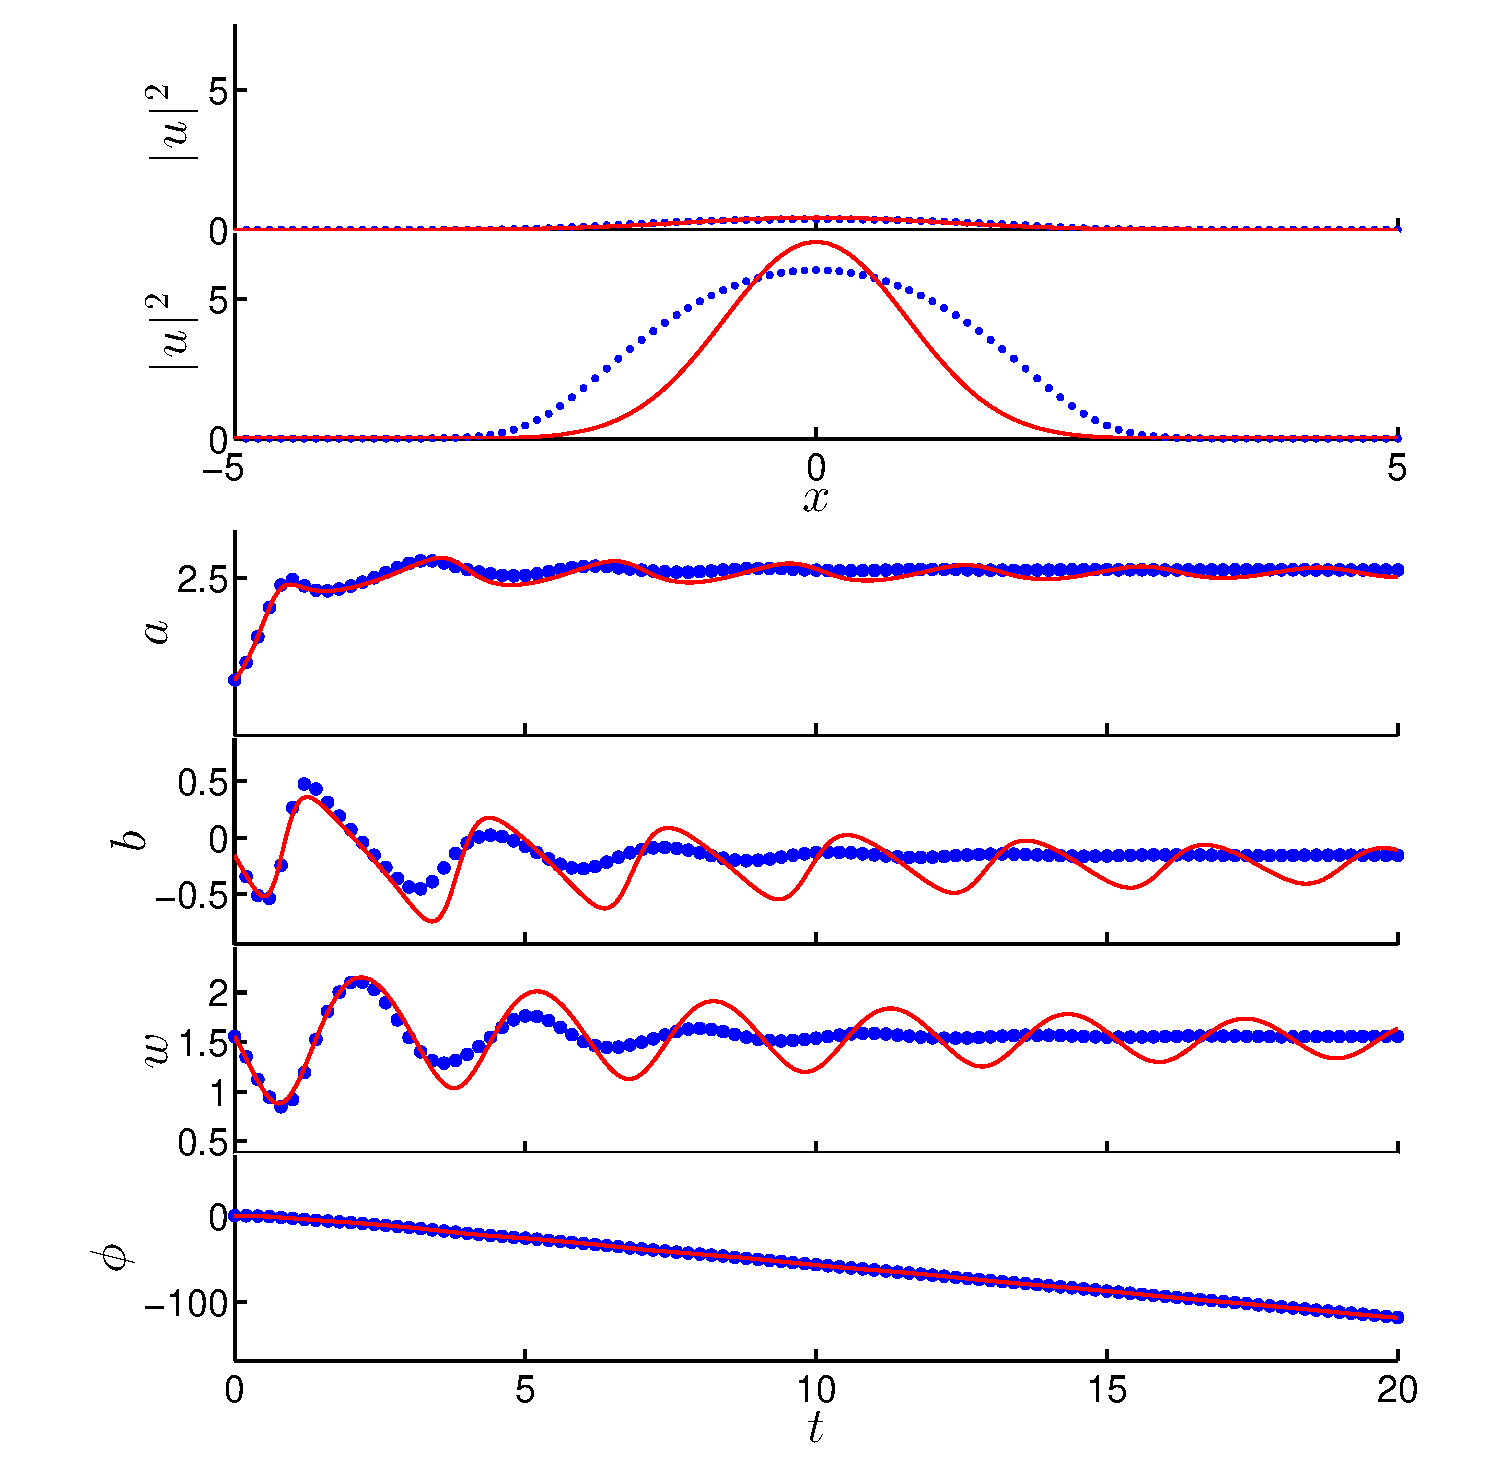
\includegraphics[width=0.8\textwidth]{Figures/Fig3a_P4_increase_v2.eps}}
  \rule{35em}{0.5pt}
\caption[Exciton-Polariton Above Equilibrium]{Evolution of the ground state of Eq.~(\ref{eq:NLSP}) starting below equilibrium in the presence of a linear spatially dependent gain (\ref{eq:gainP}) with
$\alpha =2$ and $\beta=2$, and density dependent loss of strength 
$\sigma =0.37$, as well as a harmonic potential (\ref{eq:potP}) 
of strength $\Omega = \sqrt{2}$.
%
To craft initial conditions with amplitudes below the equilibrium amplitudes we first computed the
steady state of the NLS (\ref{eq:NLSP}) which,
after projection, using least-squares fitting, into the Gaussian ansatz 
(\ref{eq:GaussAnsatz}) yields the following initial parameters:
amplitude: $a(0)= 0.6608 = a_e/4$ (four times {\em smaller} than the equilibrium solution), width:  $w(0)=1.5583$, chirp: $b(0) = -0.1563$, and phase: $\phi(0)=0.2415$.
%
Depicted are the comparison of the NCVA approximation of Eq.~(\ref{eq:NCVAP})
(red lines) with the full, numerical, NLS evolution of Eq.~(\ref{eq:NLSP})
(blue dots).
%
The top two panels depict the density $|u|^2$ at the initial time (top subpanel)
and at time $t=50$ (second subpanel).
%
The bottom four subpanels depict the evolution of the NCVA ansatz parameters
$a$, $b$, $w$, and $\phi$. For the full NLS evolution the parameters are
extracted by projecting the current solution into the NCVA ansatz using 
least-squares fitting.
\label{fig4}}
\end{figure}

\begin{figure}[htbp]
\centering
\centerline{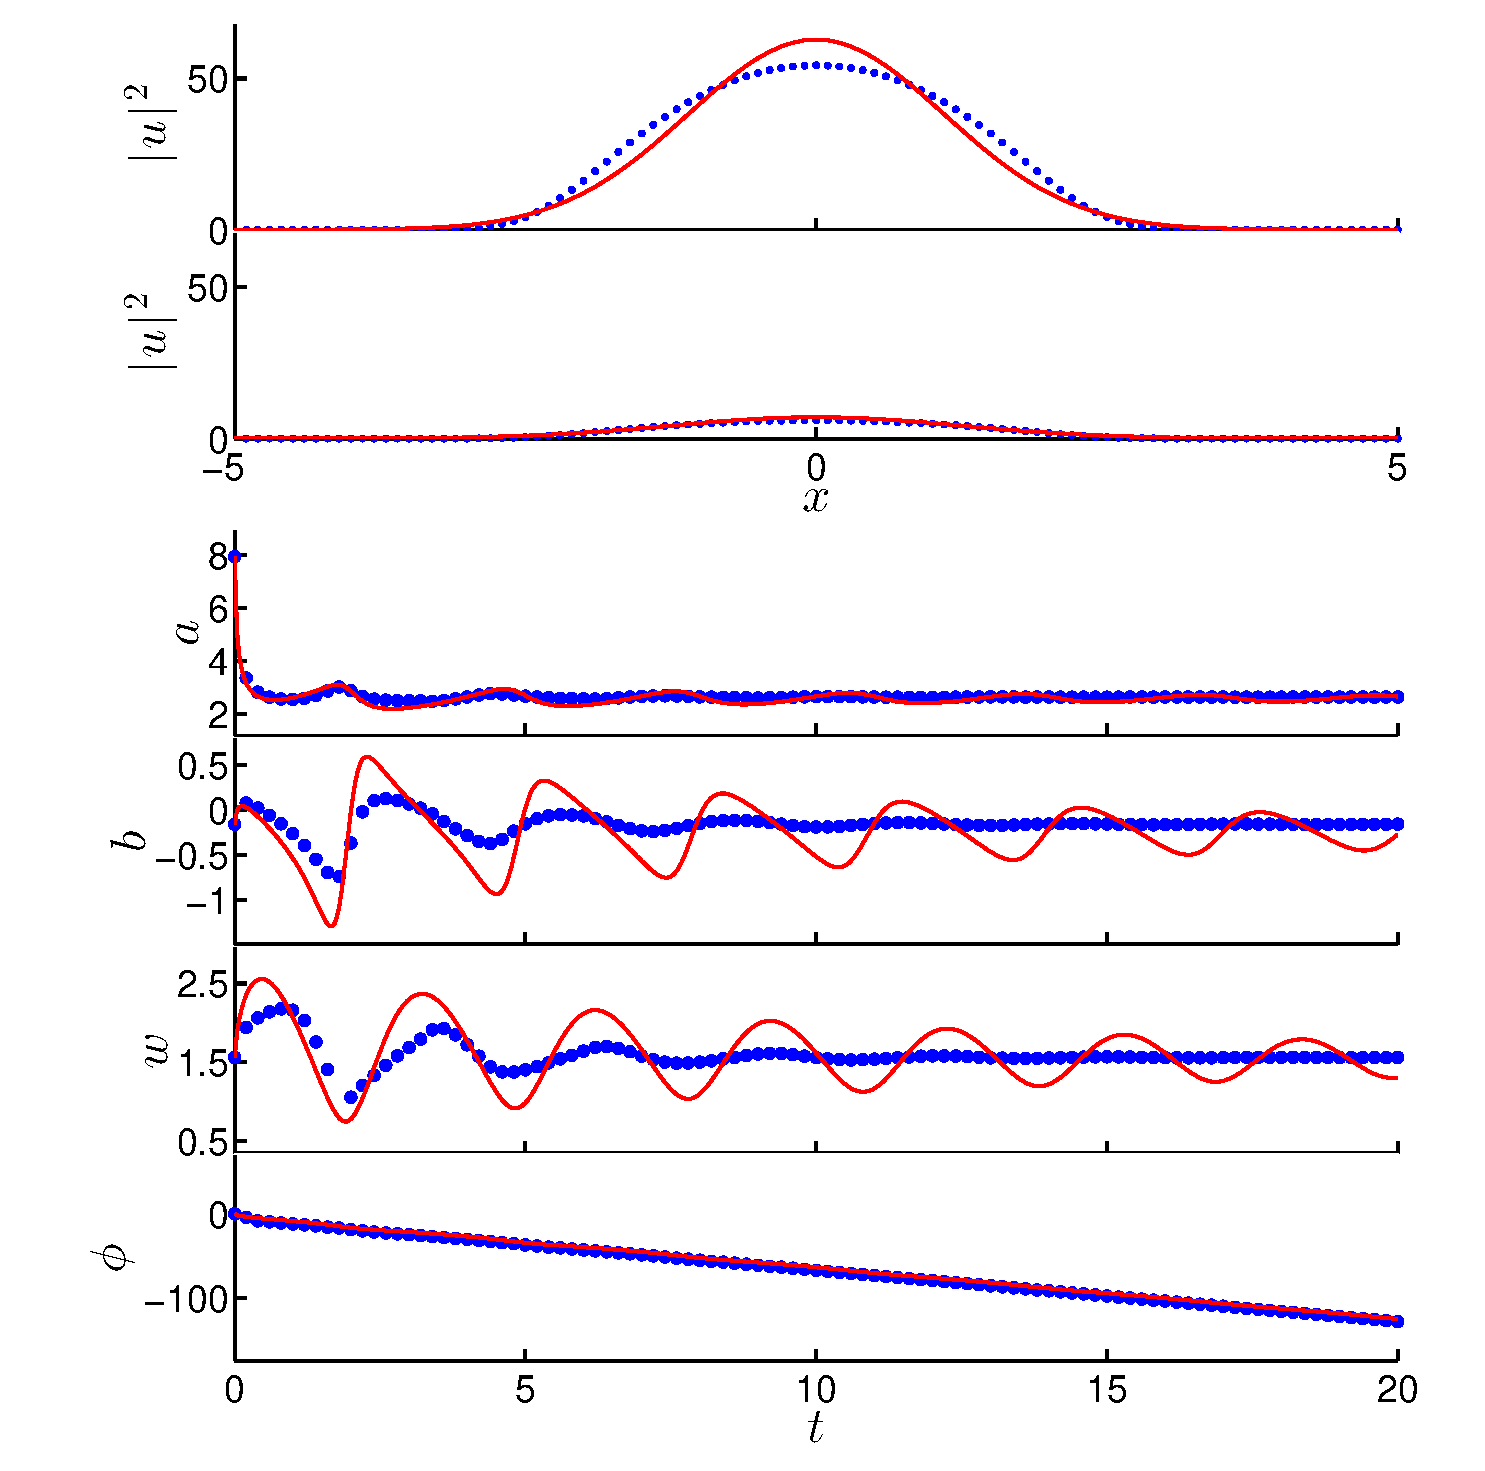
\includegraphics[width=0.8\textwidth]{Figures/Fig3b_P4_decrease_v2N.eps}}
  \rule{35em}{0.5pt}
\caption[Exciton-Polariton Below Equilibrium]{
Evolution of the ground state of Eq.~(\ref{eq:NLSP}) with the same coefficients as Fig.~\ref{fig4} starting above equilibrium
%in the presence of a linear spatially
%dependent gain (\ref{eq:gainP}) with
%$\alpha =2$ and $\beta=2$, and density dependent loss of strength 
%$\sigma =0.37$, as well as a harmonic potential (\ref{eq:potP}) 
%of strength $\Omega = \sqrt{2}$.
%
%To craft initial conditions with amplitudes above the equilibrium amplitudes we first computed the
%steady state of the NLS (\ref{eq:NLSP}) which,
%after projection, using least-squares fitting, into the Gaussian ansatz 
%(\ref{eq:GaussAnsatz}) yields the following initial parameters:
%amplitude: 
$a(0)= 7.9292 = 3 a_e$ (three times {\em larger}  than the equilibrium solution), width:  $w(0)=1.5583$, chirp: $b(0) = -0.1563$, and phase: $\phi(0)=0.2415$.
%
The layout of the panels is the same as in the previous Fig.~\ref{fig4}.
\label{fig5}}
\end{figure}

%\begin{figure}[htbp]
% \centering
%  \centerline{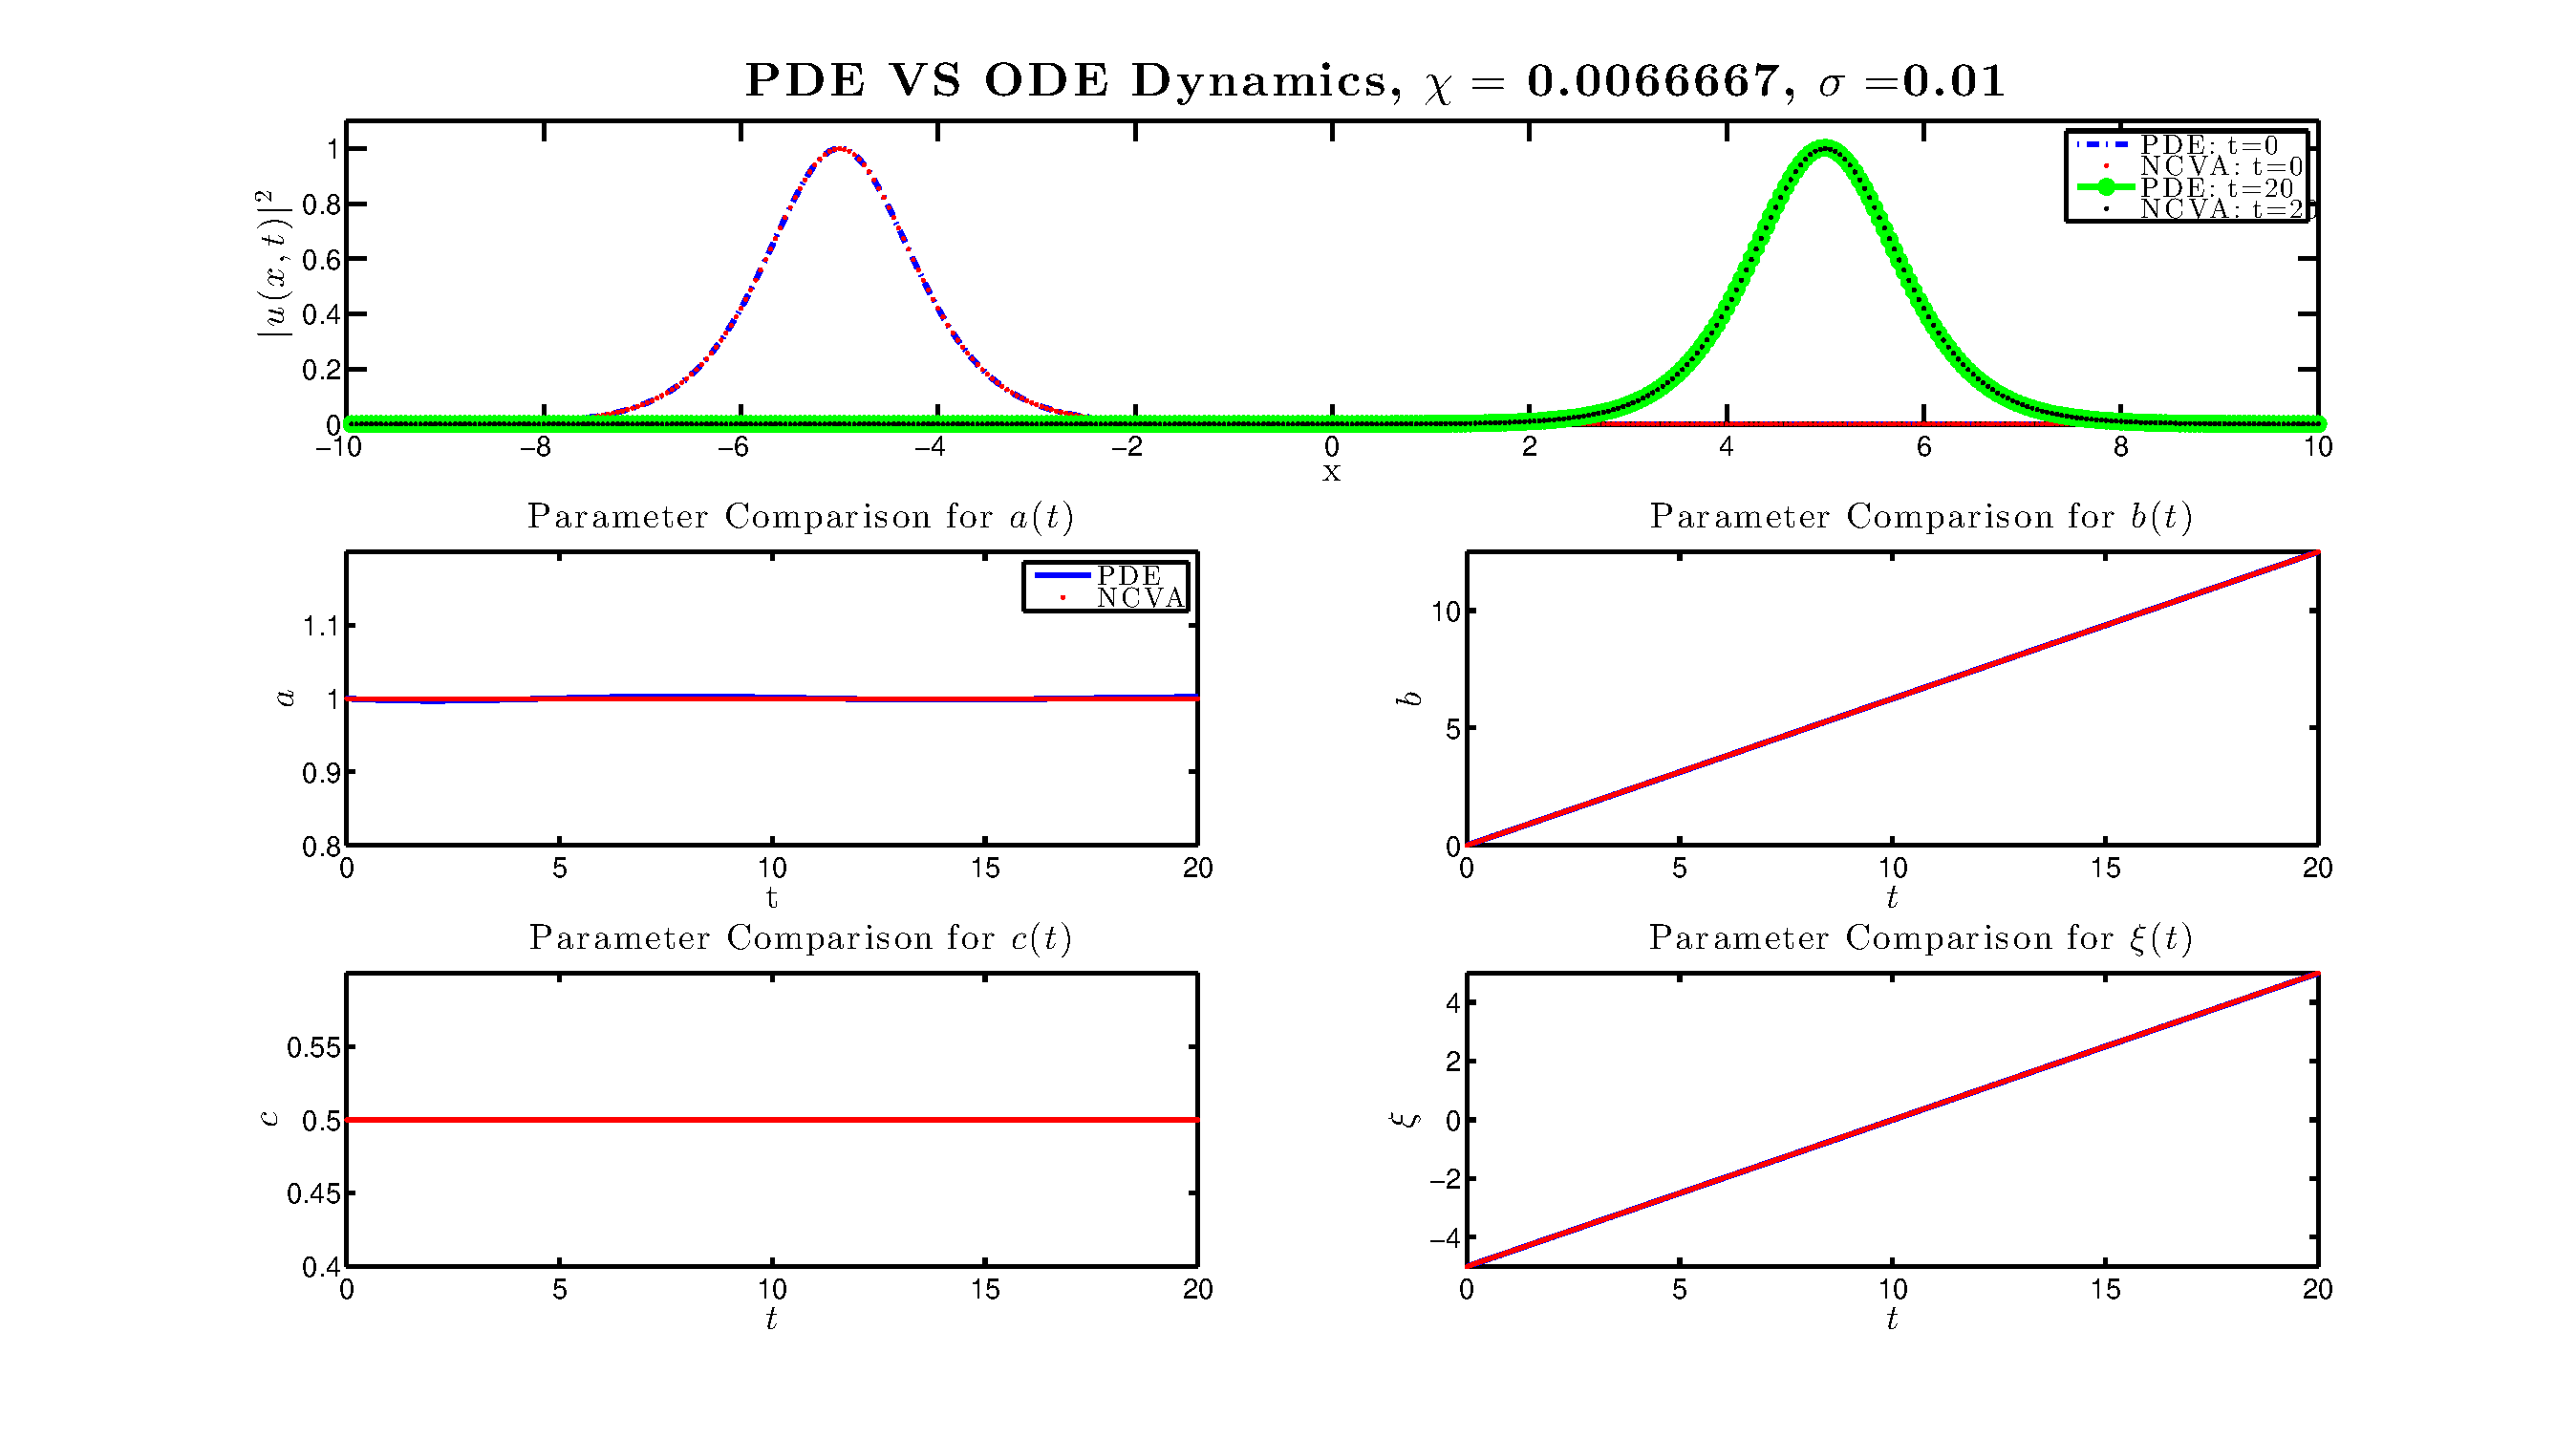
\includegraphics[width=1.2\textwidth, height=\textwidth]{EP001.eps}}
%  \rule{35em}{0.5pt}
%  \caption[Exciton-Polariton Condensate: NLS with Linear Gain $\sigma = 0.01$ and Density Dependent Loss $\chi=(2/3) \sigma$ ]{{\bf Exciton-Polariton Condensate:} Comparison of ODE dynamics for the parameters $a$, $b$, $c$, and $\xi$ between forward integration of the PDE and the NCVA with $\chi=(2/3) \sigma$ and $\sigma = 0.01$.}
%   \label{fig:Ploss001}
%\end{figure}
%
%
%\begin{figure}[htbp]
%  \centering
%  \centerline{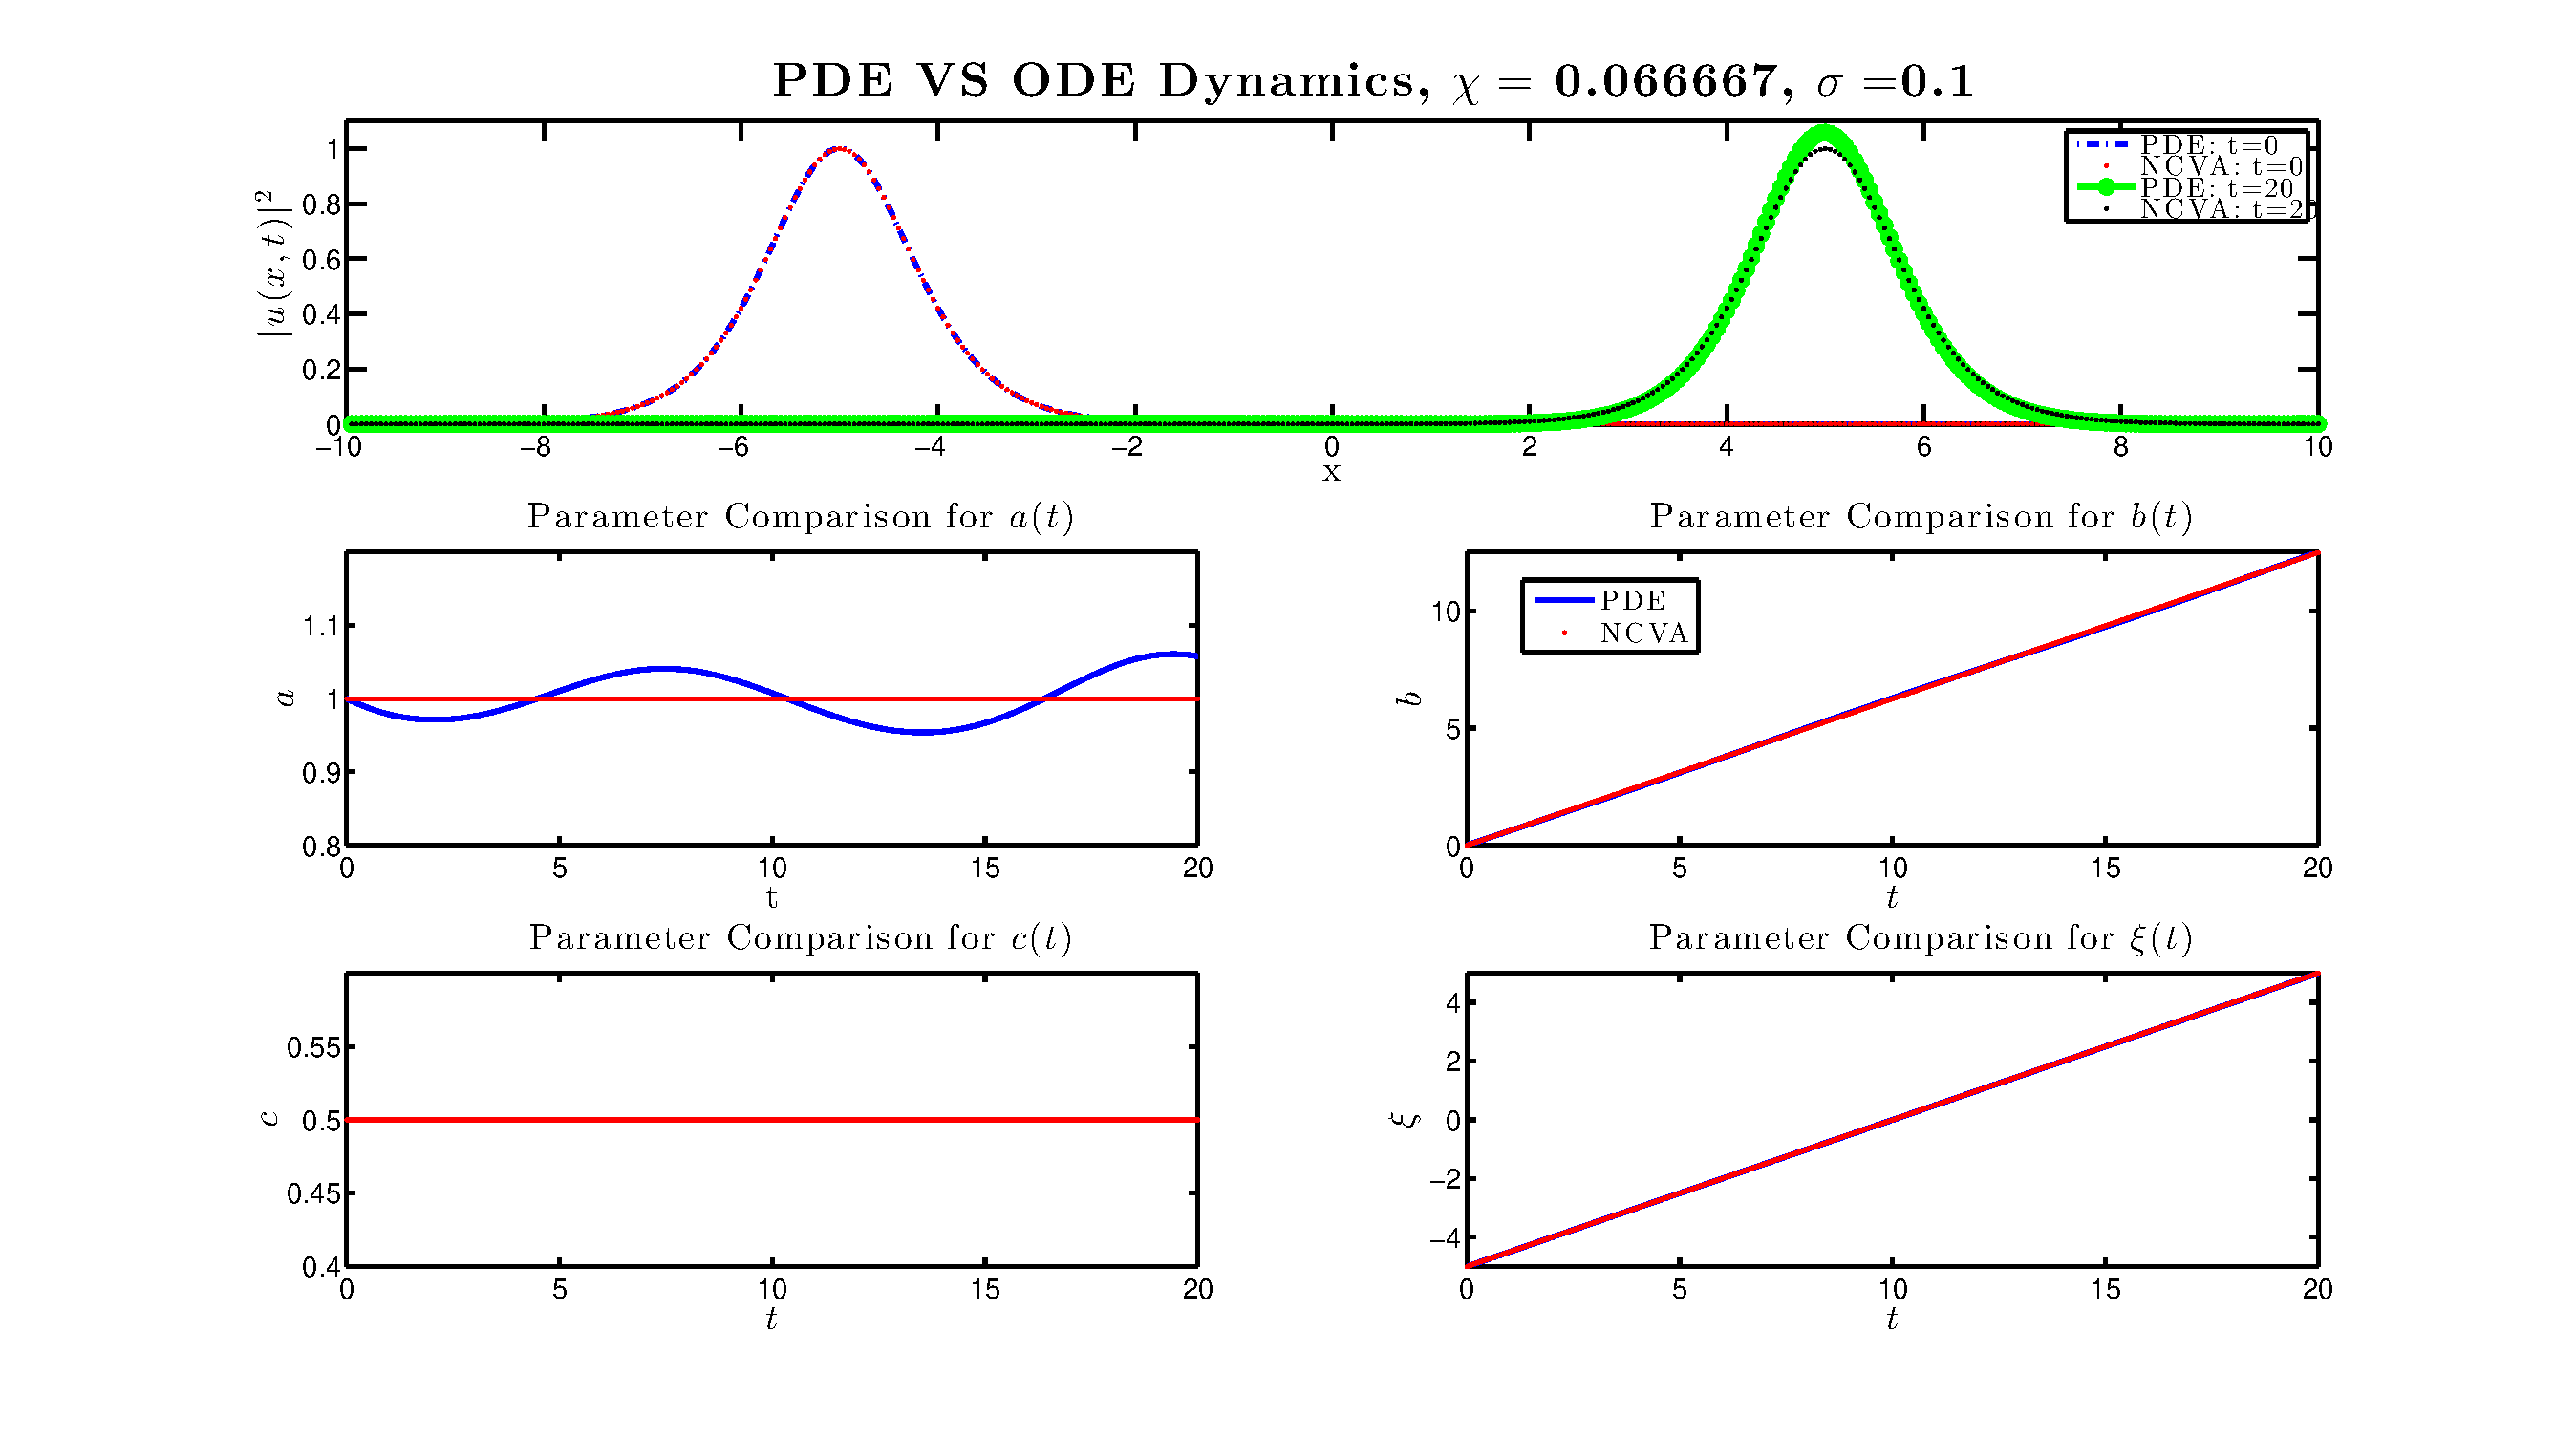
\includegraphics[width=1.2\textwidth, height=\textwidth]{EP01.eps}}
%  \rule{35em}{0.5pt}
%  \caption[Exciton-Polariton Condensate: NLS with Linear Gain $\sigma = 0.1$ and Density Dependent Loss $\chi=(2/3) \sigma$]{{\bf Exciton-Polariton Condensate:} Comparison of ODE dynamics for the parameters $a$, $b$, $c$, and $\xi$ between forward integration of the PDE and the NCVA with $\chi=(2/3) \sigma$ and $\sigma = 0.1$.}
%   \label{fig:Ploss01}
%\end{figure}
%
%\begin{figure}[htbp]
%\centering
%\begin{subfigure}[t]{0.49\textwidth}
%  		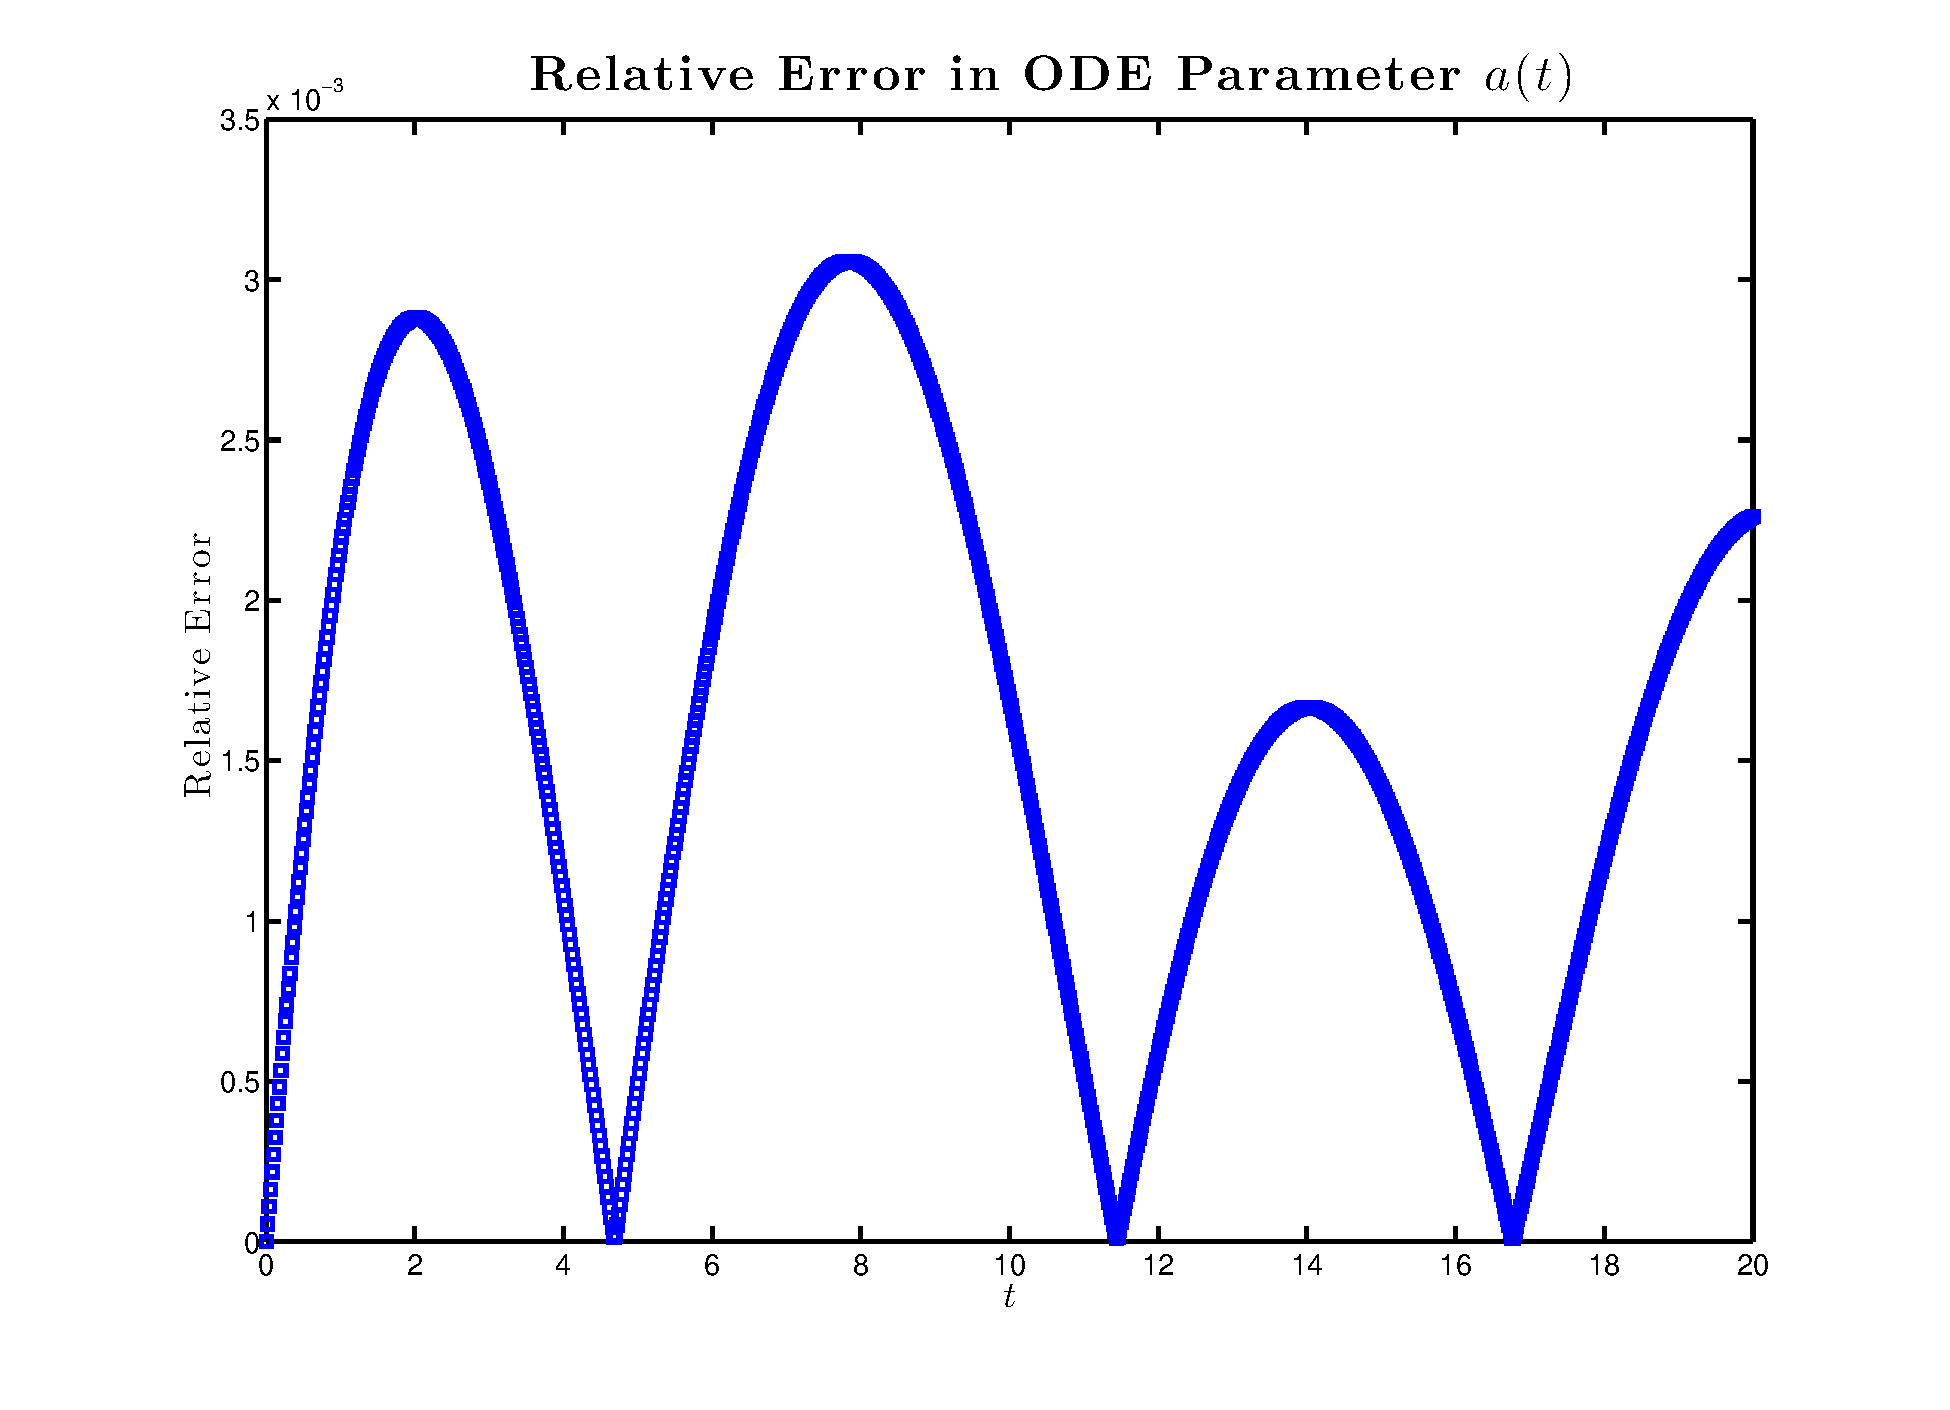
\includegraphics[width=\textwidth, height = \textwidth]{EP001relativeerror.eps}
%	         \caption{Relative error between NCVA and PDE parameter $a(t)$ values for $\sigma=0.01$.}
%	         \label{fig:PLoss001Err}
%	     \end{subfigure}
%  \begin{subfigure}[t]{0.49\textwidth}
%  		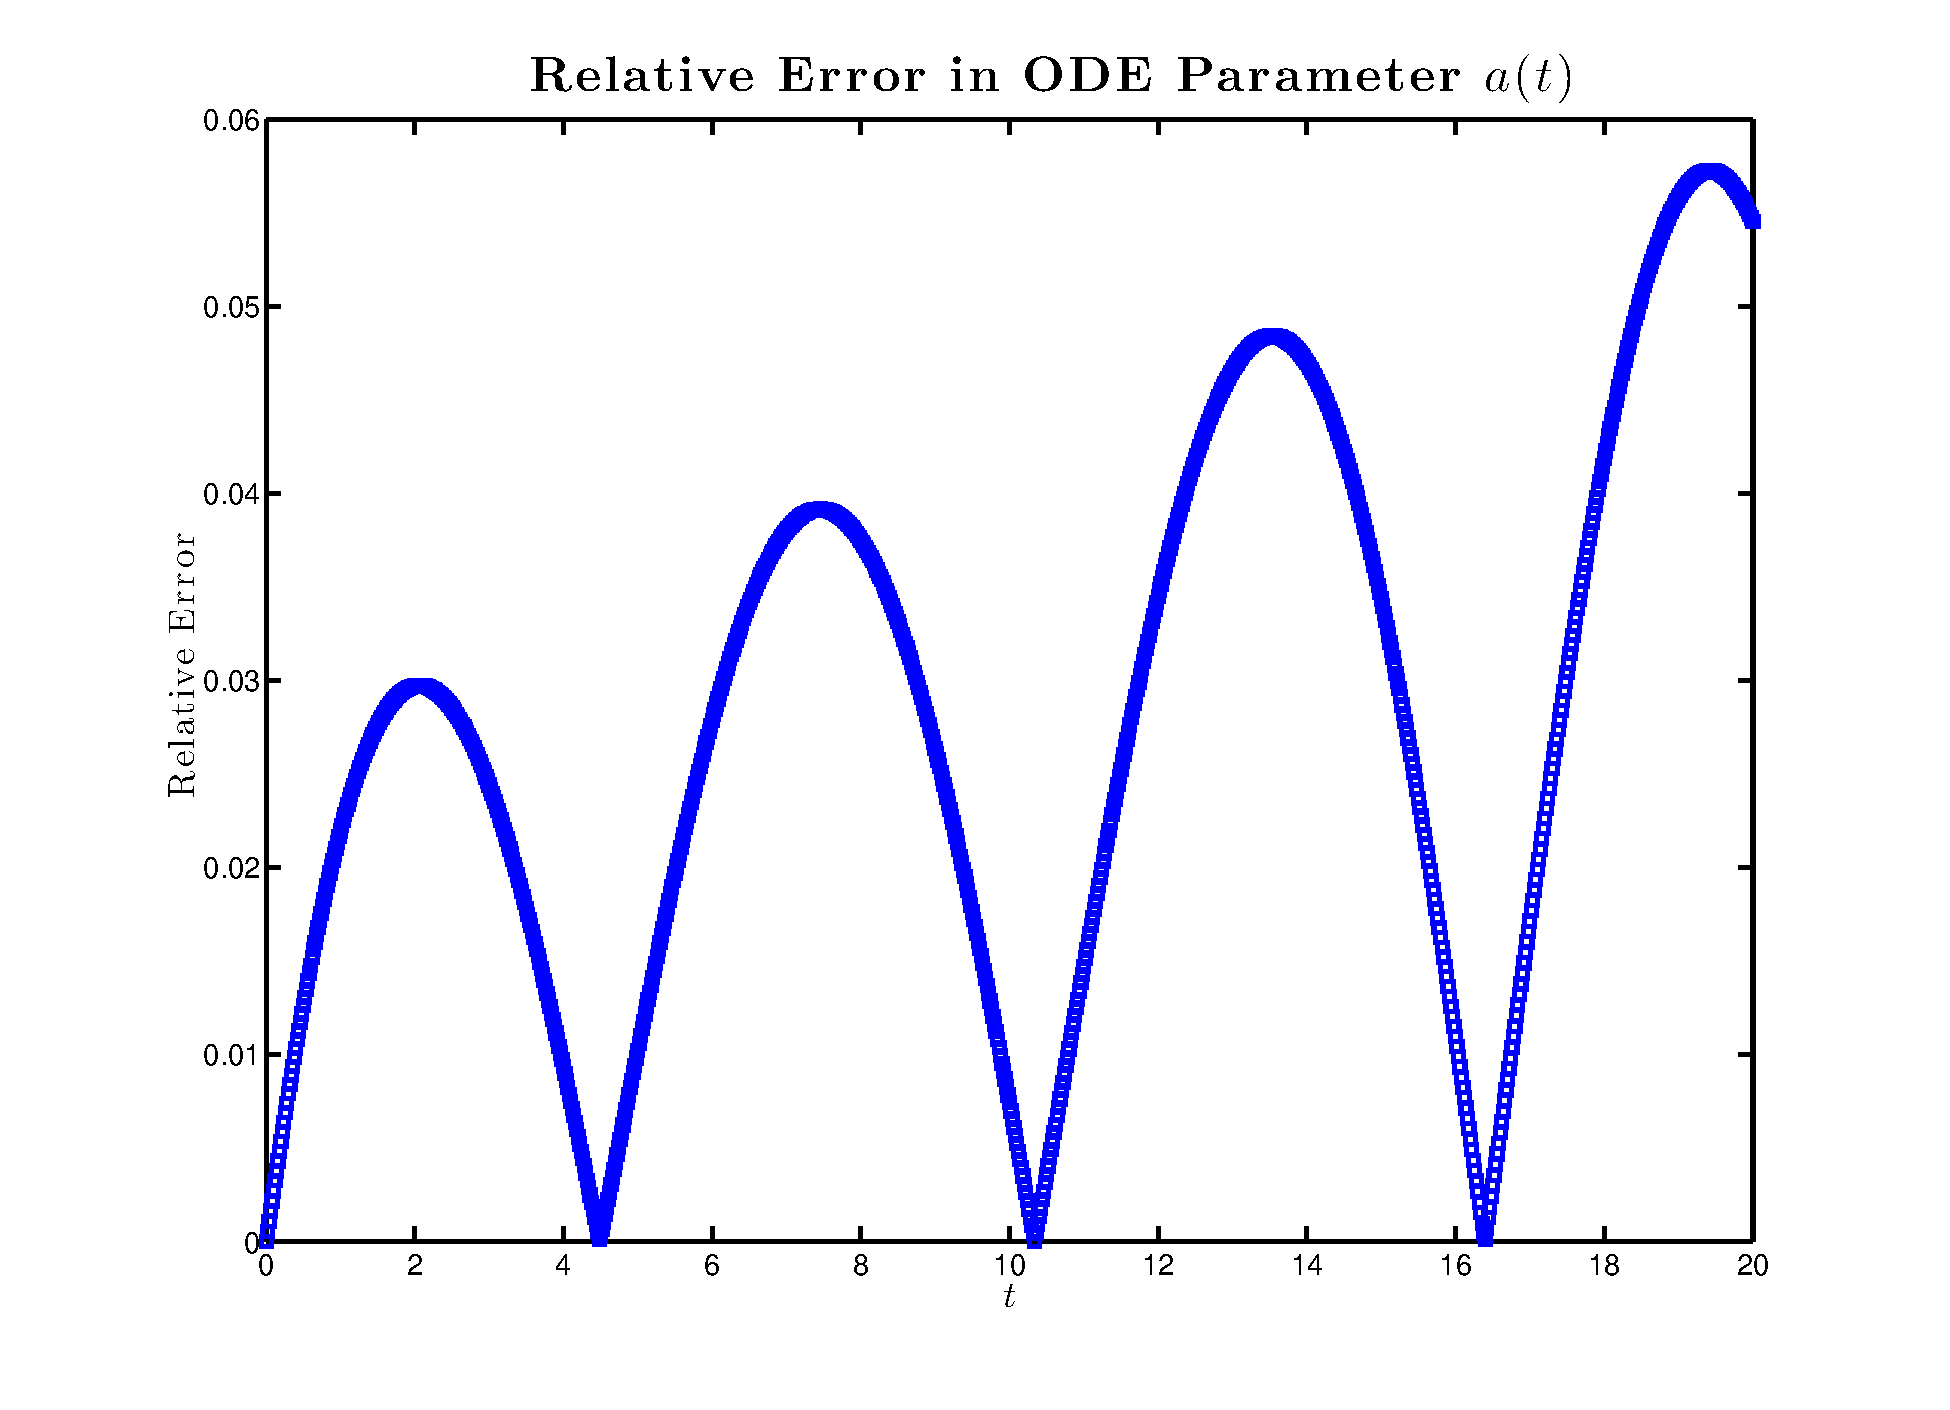
\includegraphics[width= \textwidth, height = \textwidth]{EP01relativeerror.eps}  
%	          \caption{Relative error between NCVA and PDE parameter $a(t)$ values for $\sigma=0.1$.}
%	         \label{fig:PLoss01Err}
%	    \end{subfigure} 
%  \rule{35em}{0.5pt}
%   \caption[Relative Error in Amplitude for Exciton-Polariton Condensate: NLS with Linear Gain and Density Dependent Loss $\chi=(2/3) \sigma$]{{\bf Exciton-Polariton Condensate:} Amplitude parameter $a(t)$ relative error for $\chi=(2/3) \sigma$ where (A) $\sigma=0.01$ and (B) $\sigma=0.1$.}
%   \label{fig:PlossA}
%\end{figure}

%\clearpage
%
%The equilibrium shown in the examples above [Figs.~\ref{fig:Ploss001} and \ref{fig:Ploss01}] illustrate the dynamics of constant exciton pumping and loss of polaritons.  The interesting cases occur when the system is set far from the equilibrium point $a$ = 1.  We start with $a_0 = 1$ and show the soliton decaying to the equilibrium height $a$ = 1 over time $t\in[0,500]$ in Fig.~\ref{fig:Pdecay}.  The numerics were performed the same as above except $\xi_0 = -25$.  The relative error in the height for $a$ is on the order of $10^{-3}$ and increases to $10^{-2}$ over time in Fig.~\ref{fig:PdecayErr}.  The ODE and PDE solutions agree very well with the soliton solution decaying to the fixed point $a$ = 1.  The numerical oscillations of the PDE as time increases is believed to be an artifact of the fitting routine and more analysis will be performed.    
%
%In Fig.~\ref{fig:Pgain}, we start at a height $a$ less than the fixed point, $a_0$ = 0.5 such that the PDE and ODE solution will grow and eventually reach the fixed point $a =1$.  The same numeric parameters are used as before except $\xi_0 = -15$ and $t\in[0,300]$.  The relative error in the height for $a$ is on the order of $10^{-2}$ in Fig.~\ref{fig:PgainErr}.  The non-conserved system is well described by the NCVA equations of motion for the time-dependent parameters $a$, $b$, $c$, and $\xi$ especially when considering constant pumping in of excitons and decay (loss) of polaritons due to their short lifespan.

%\begin{figure}[htbp]
% \centering
%  \centerline{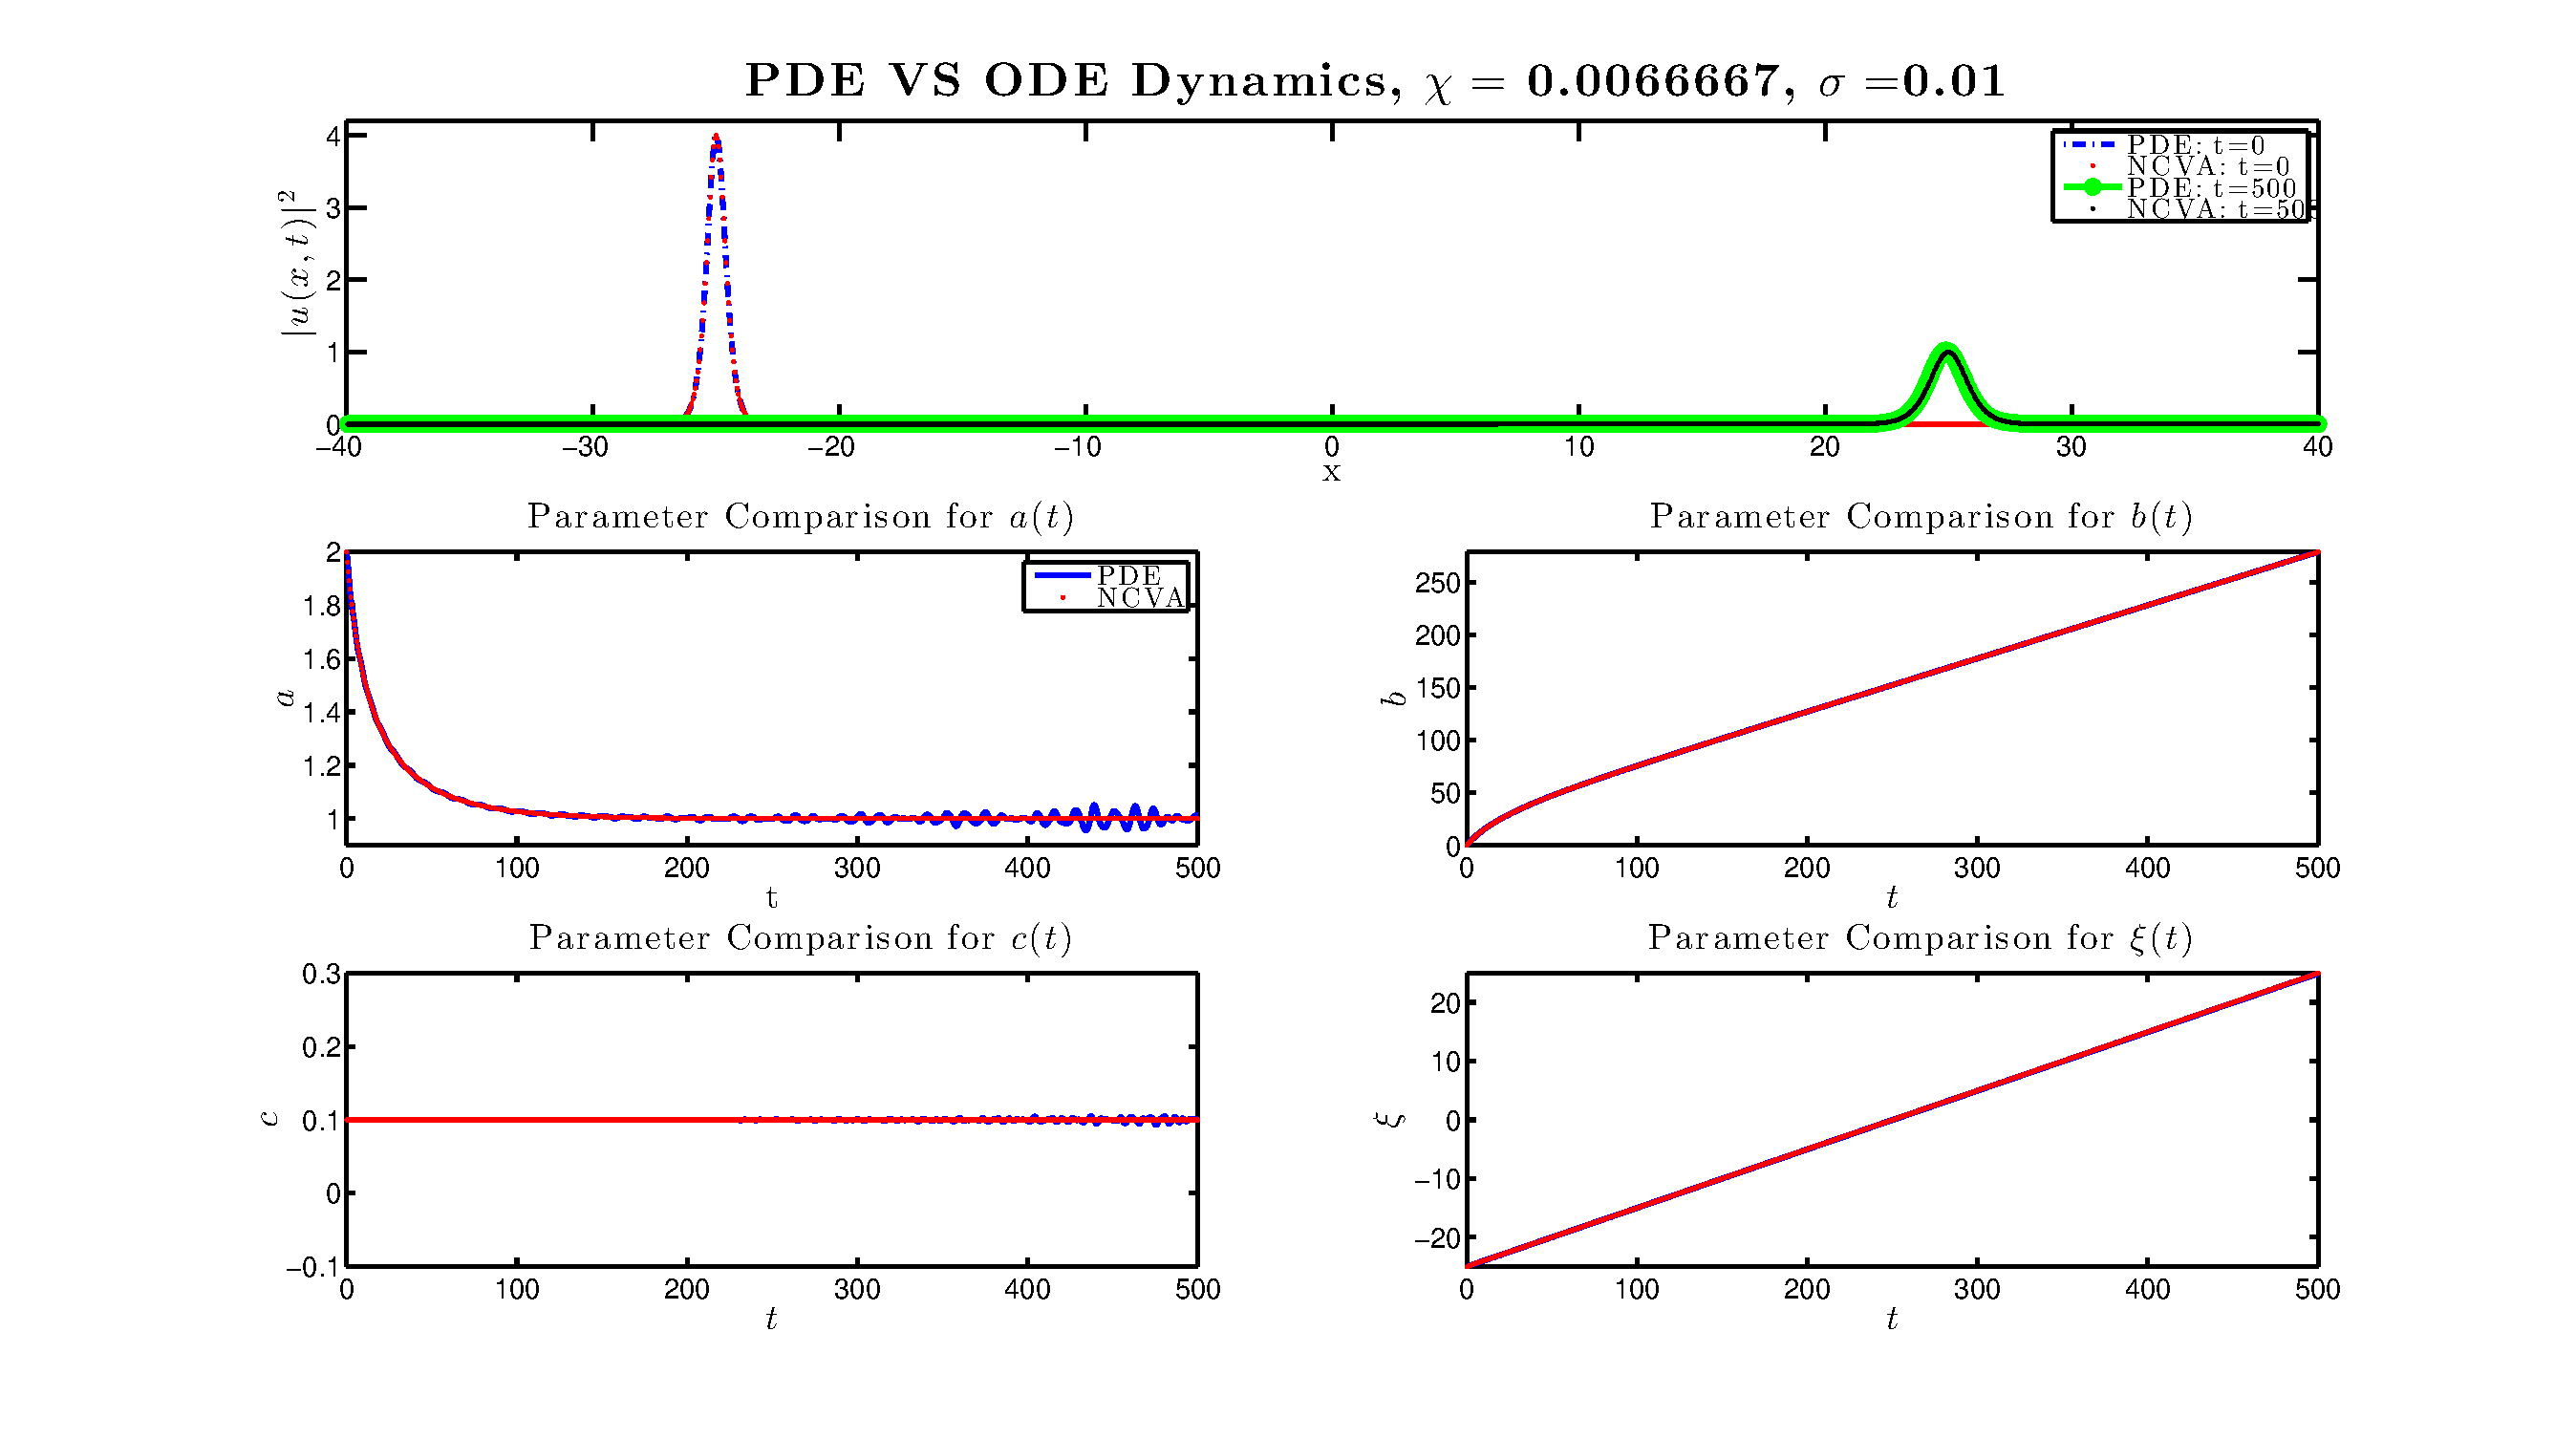
\includegraphics[width=1.2\textwidth, height=\textwidth]{EPdecay.eps}}
%  \rule{35em}{0.5pt}
%  \caption[Exciton-Polariton Condensate: NLS with Linear Gain $\sigma = 0.01$ and Density DependentLoss $\chi=(2/3) \sigma$ for $a_0 = 2$ ]{{\bf Exciton-Polariton Condensate:} Comparison of ODE dynamics for the parameters $a$, $b$, $c$, and $\xi$ between forward integration of the PDE and the NCVA with $\chi=(2/3) \sigma$ and $\sigma = 0.01$ starting at $a_0 = 2$.}
%   \label{fig:Pdecay}
%\end{figure}
%
%
%\begin{figure}[htbp]
%  \centering
%  \centerline{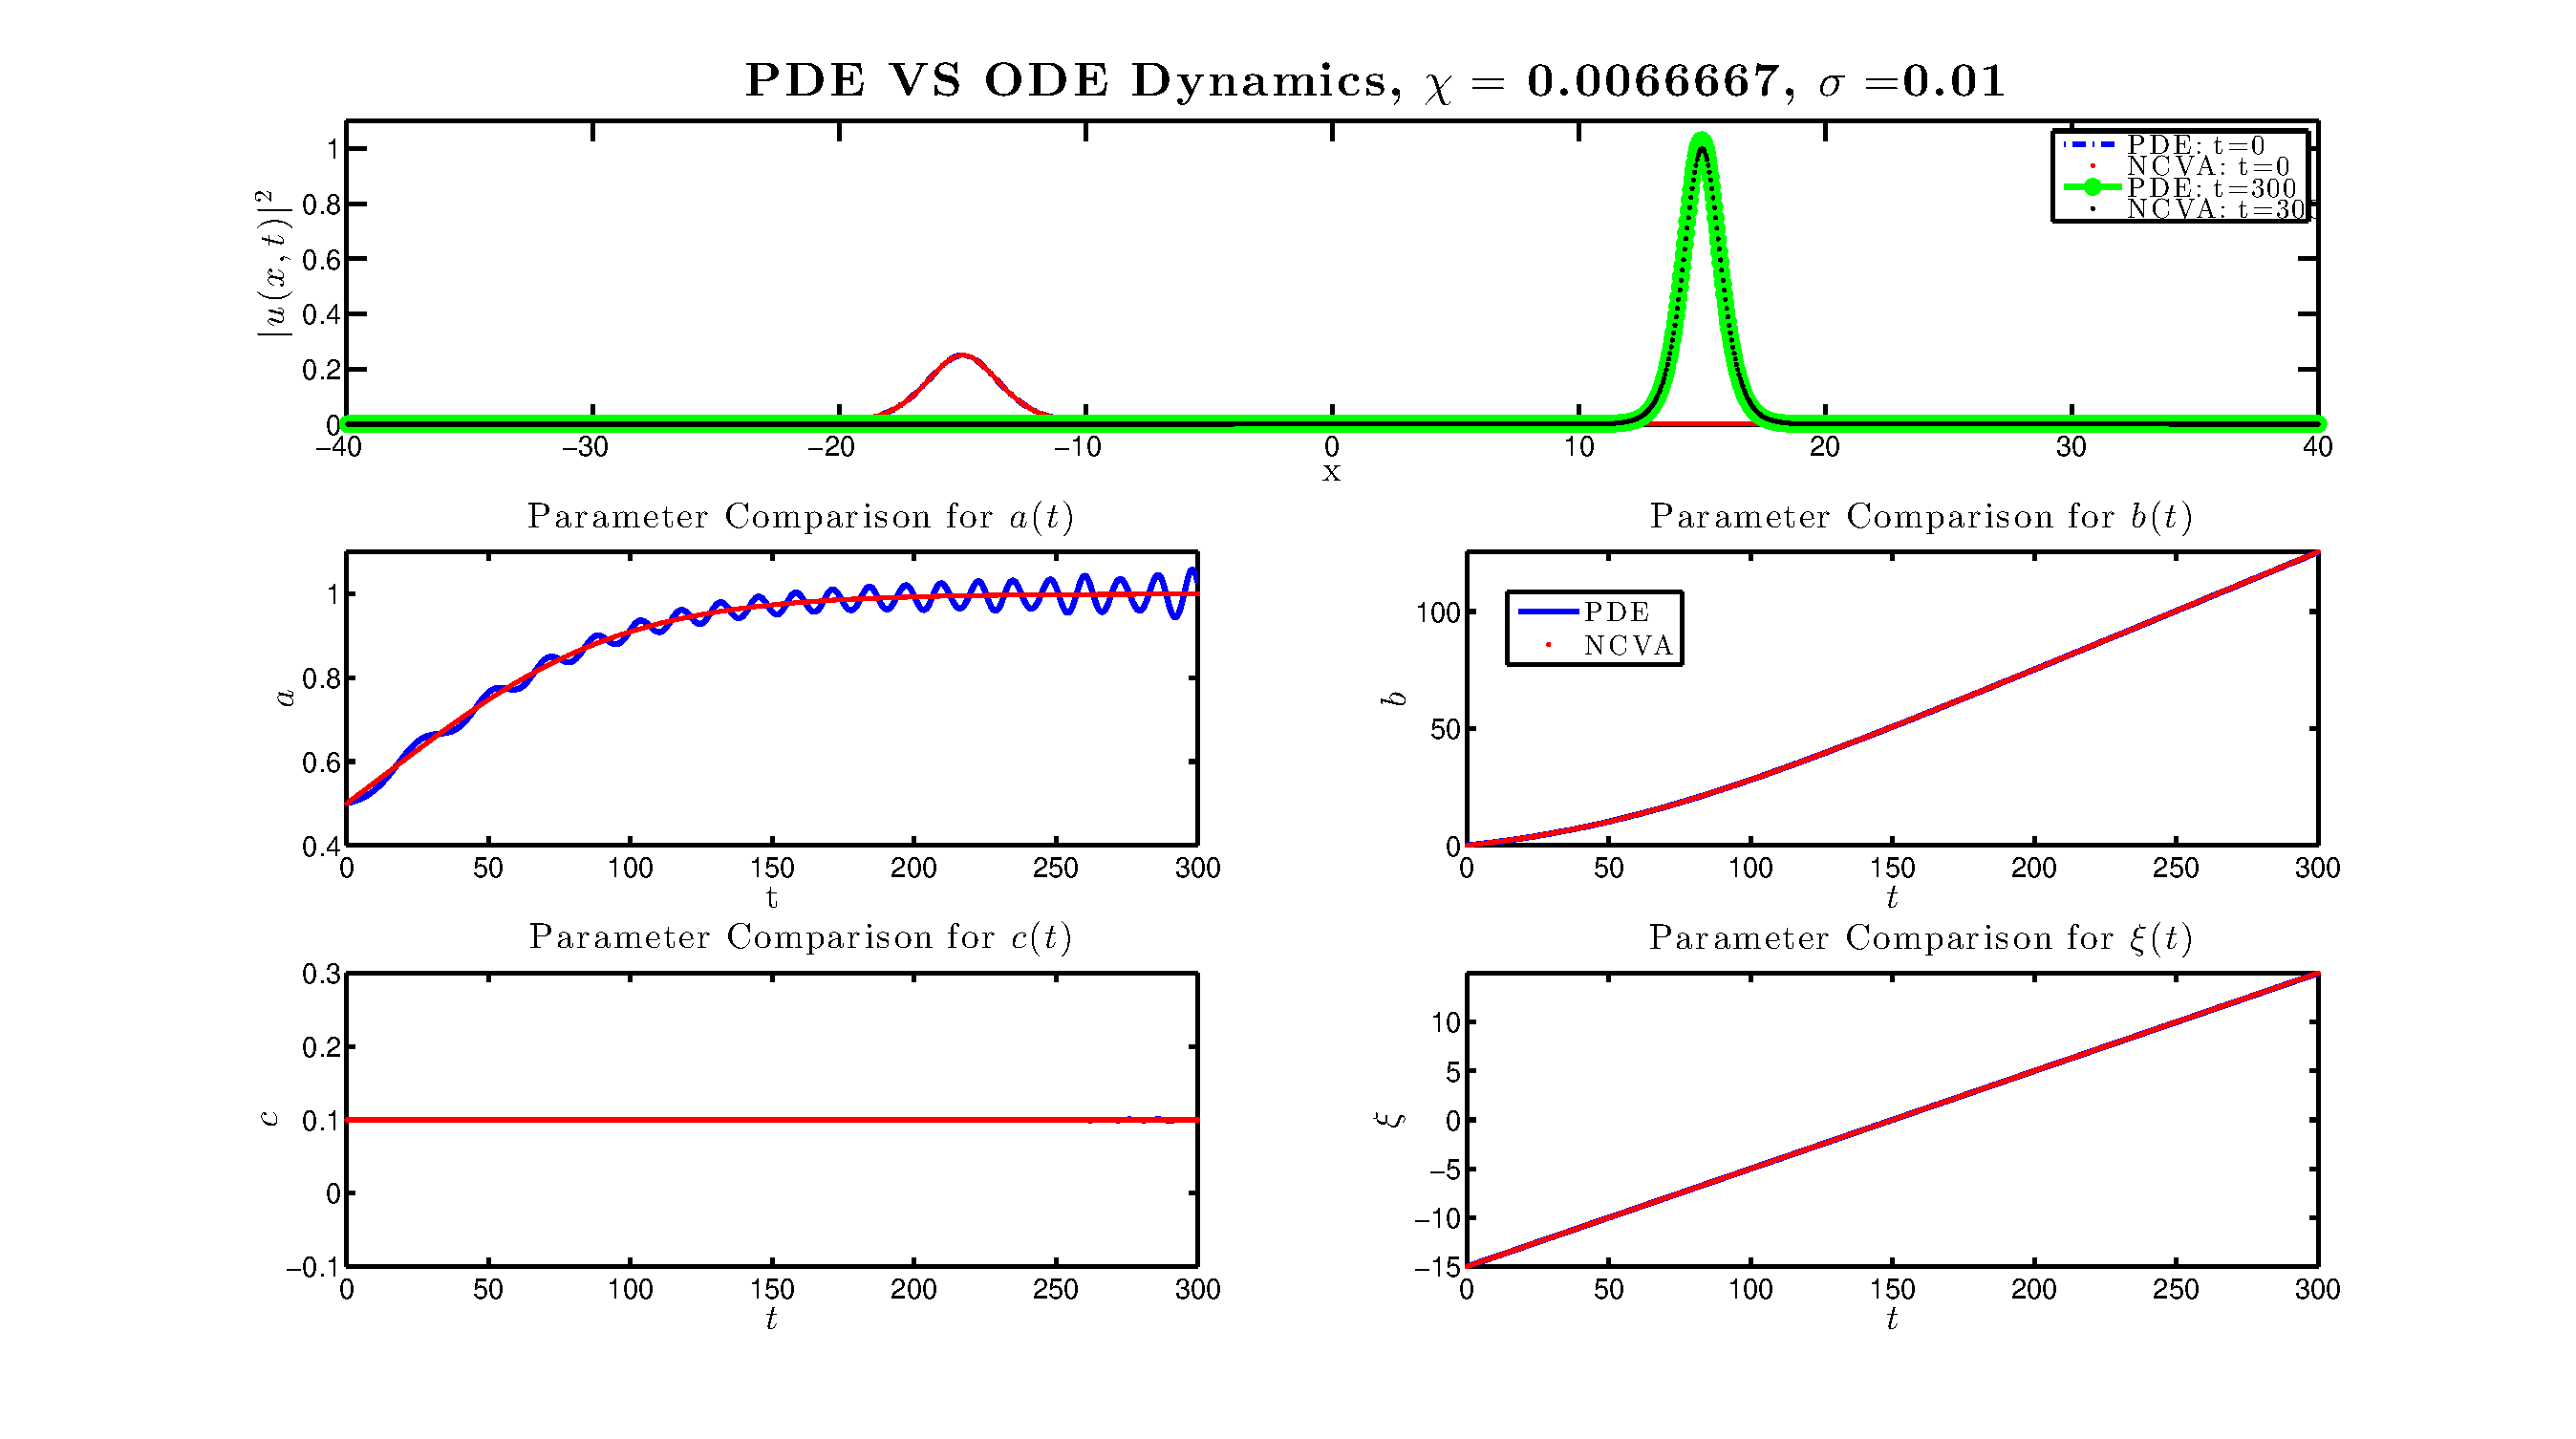
\includegraphics[width=1.2\textwidth, height=\textwidth]{EPgain.eps}}
%  \rule{35em}{0.5pt}
%  \caption[Exciton-Polariton Condensate: NLS with Linear Gain $\sigma = 0.01$ and Density Dependent Loss $\chi=(2/3) \sigma$ for $a_0 = 0.5$]{{\bf Exciton-Polariton Condensate:} Comparison of ODE dynamics for the parameters $a$, $b$, $c$, and $\xi$ between forward integration of the PDE and the NCVA with $\chi=(2/3) \sigma$ and $\sigma = 0.01$ starting at $a_0 = 0.5$.}
%   \label{fig:Pgain}
%\end{figure}
%
%\begin{figure}[htbp]
%\centering
%\begin{subfigure}[t]{0.49\textwidth}
%  		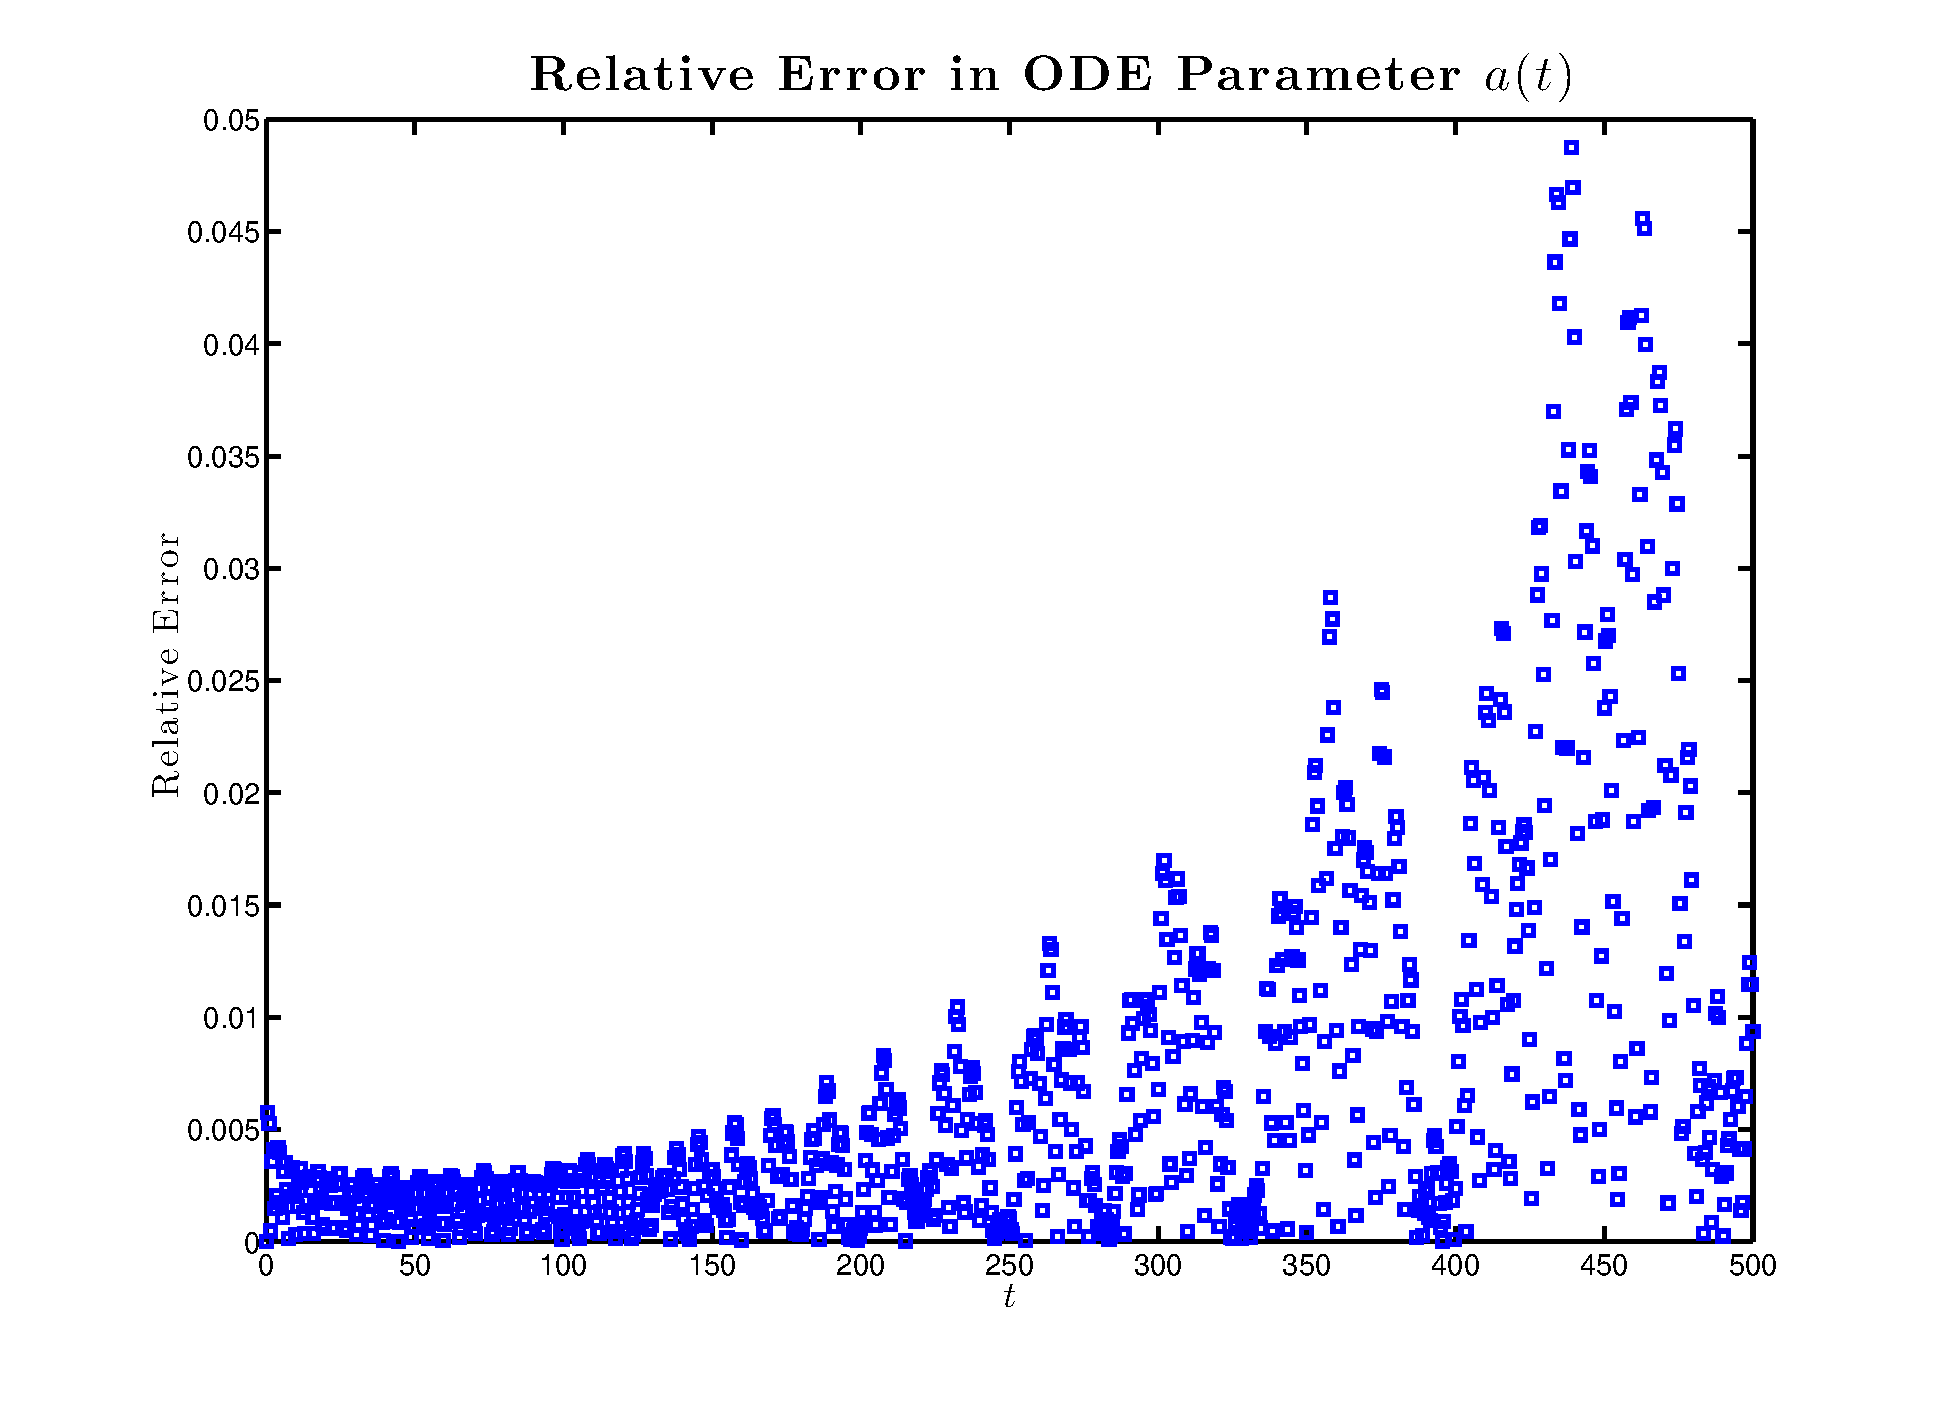
\includegraphics[width=\textwidth, height = \textwidth]{EPdecayrelativeerror.eps}
%	         \caption{Relative error between NCVA and PDE parameter $a(t)$ values for $a_0=2$.}
%	         \label{fig:PdecayErr}
%	     \end{subfigure}
%  \begin{subfigure}[t]{0.49\textwidth}
%  		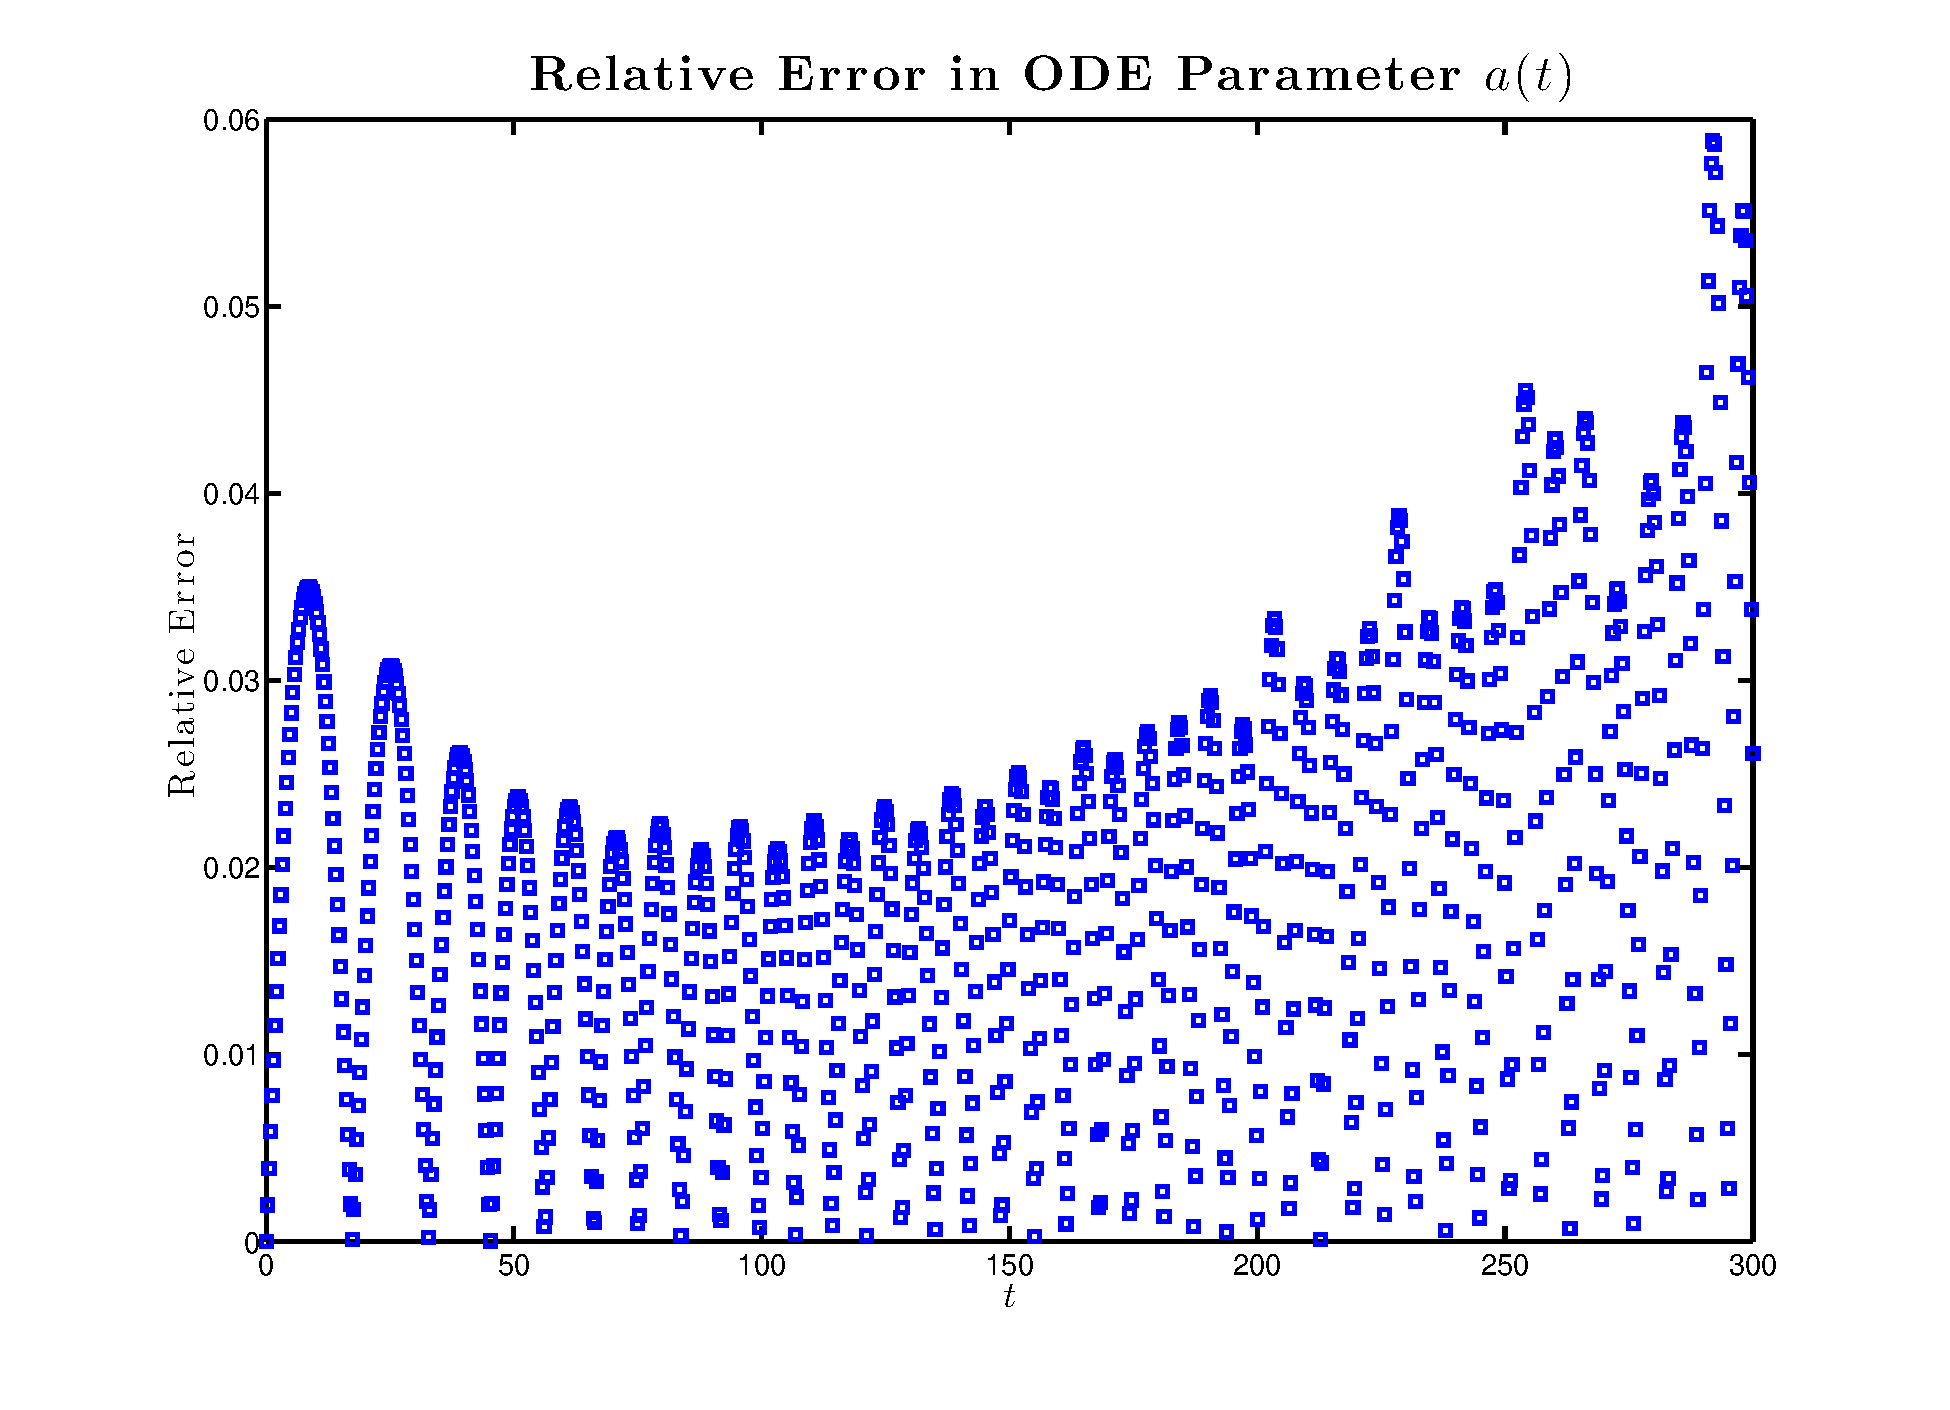
\includegraphics[width= \textwidth, height = \textwidth]{EPgainrelativeerror.eps}  
%	          \caption{Relative error between NCVA and PDE parameter $a(t)$ values for $a_0 = 0.5$.}
%	         \label{fig:PgainErr}
%	    \end{subfigure} 
%  \rule{35em}{0.5pt}
%   \caption[Relative Error in Amplitude for Exciton-Polariton Condensate: NLS with Linear Gain and Density Dependent Loss $\chi=(2/3) \sigma$]{{\bf Exciton-Polariton Condensate:} Amplitude parameter $a(t)$ relative error for $\chi=(2/3) \sigma$, $\sigma = 0.01$ where (A) $a_0 = 2$ and (B) $a_0=0.5$.}
%   \label{fig:Peq}
%\end{figure}

%\clearpage

%\begin{figure}[htbp]
%\centering
%\begin{subfigure}[t]{0.49\textwidth}
%  		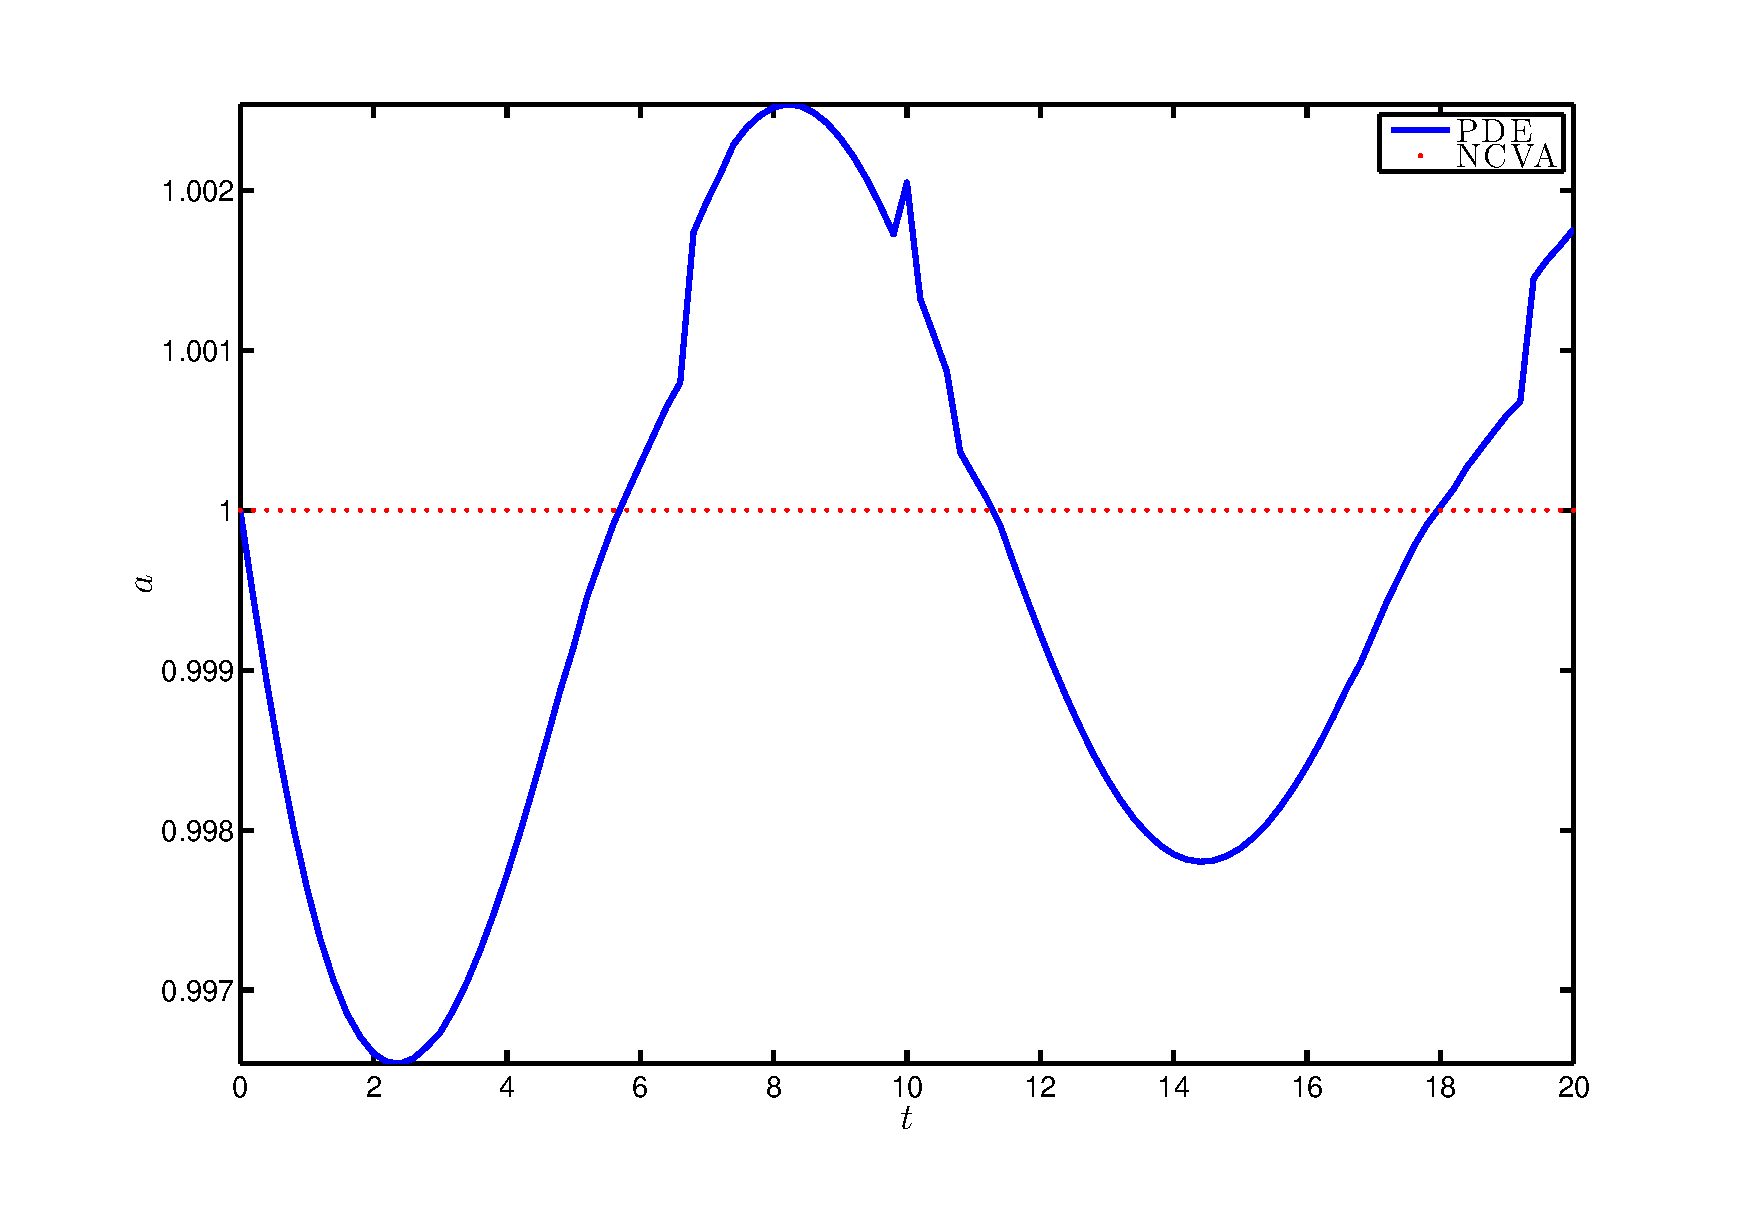
\includegraphics[width=\textwidth, height = \textwidth]{PE001a.eps}
%	         \caption{Amplitude parameter comparison $a(t)$ between PDE and NCVA solutions.}
%	         \label{fig:PLoss001a}
%	     \end{subfigure}
%  \begin{subfigure}[t]{0.49\textwidth}
%  		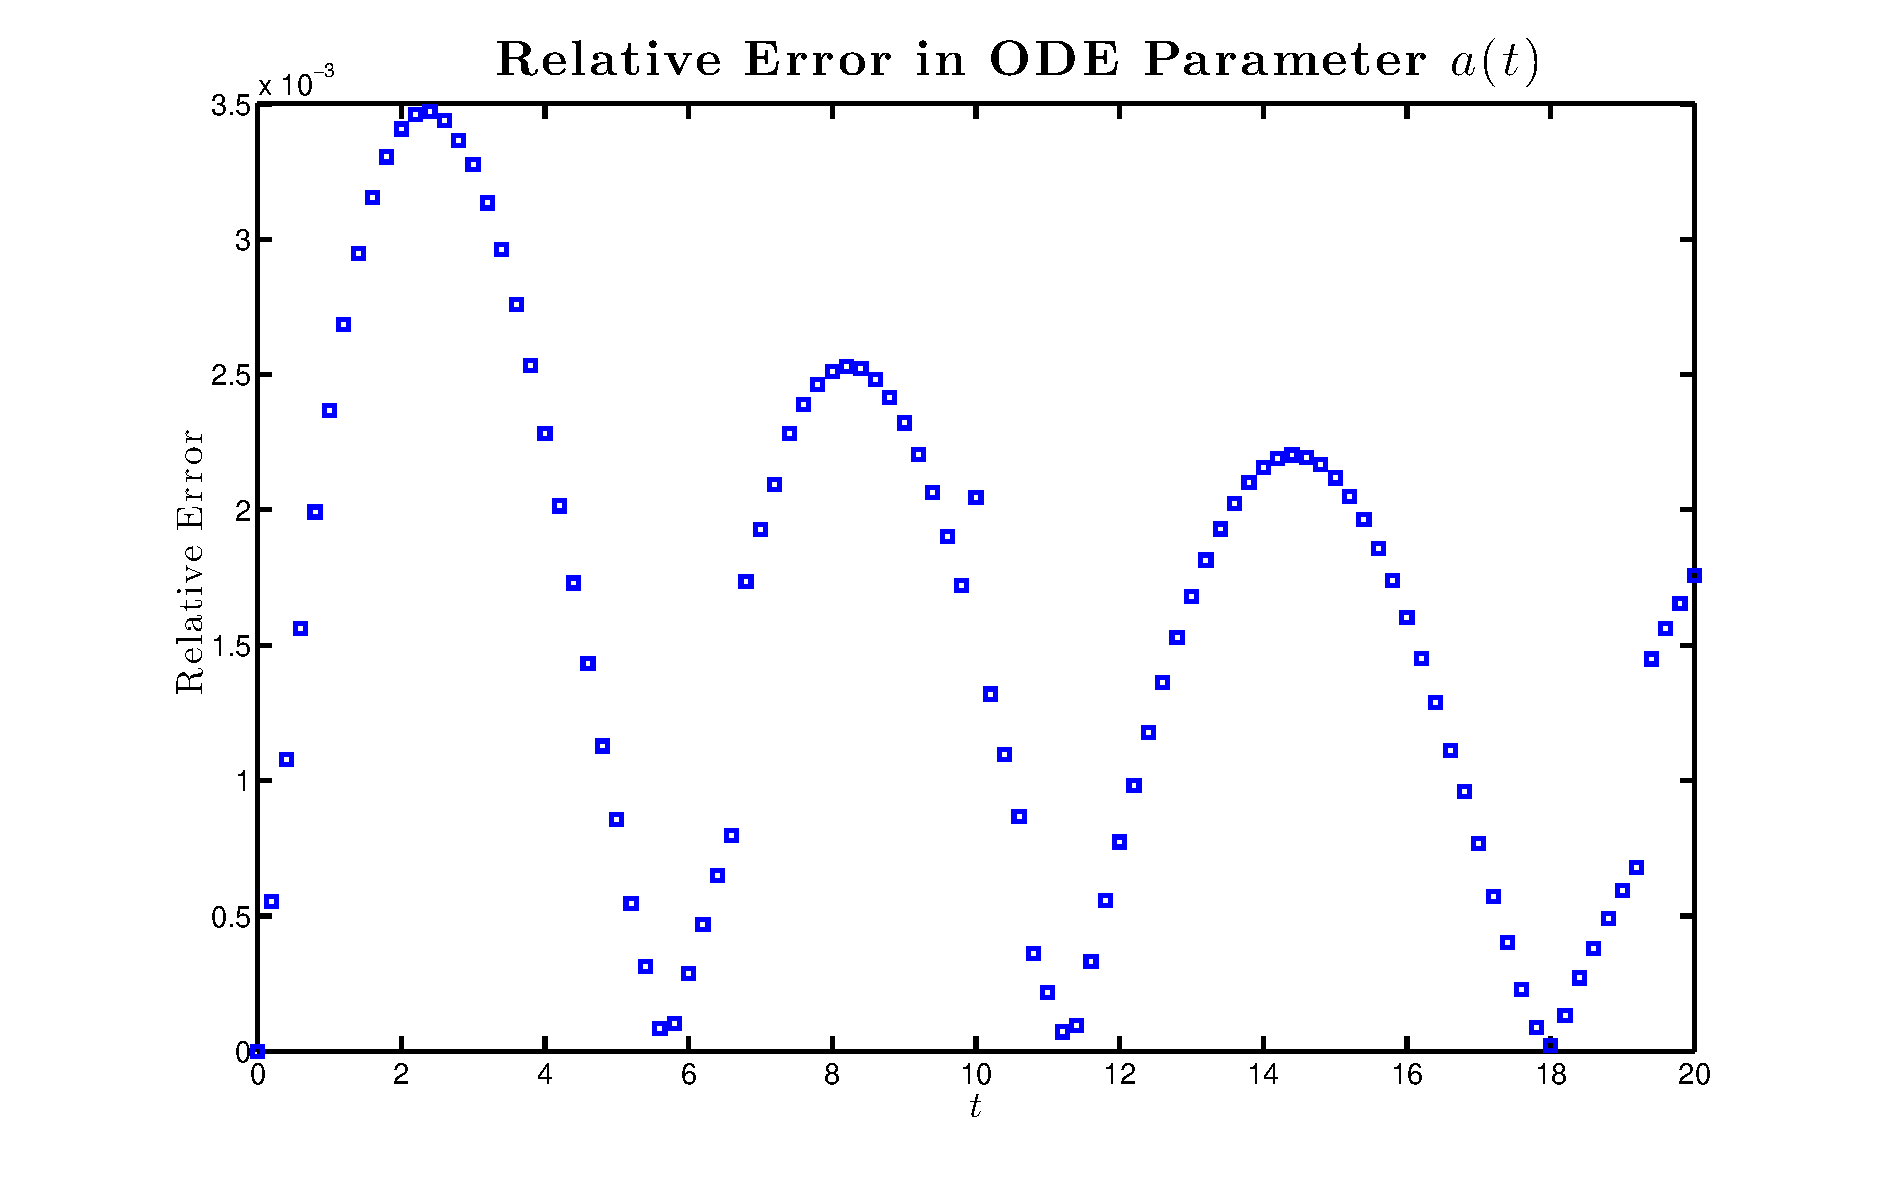
\includegraphics[width= \textwidth, height = \textwidth]{PE001relativeError.eps}  
%	          \caption{Relative error between NCVA and PDE parameter $a(t)$ values.}
%	         \label{fig:PLoss001Err}
%	    \end{subfigure} 
%  \rule{35em}{0.5pt}
%   \caption[Exciton-Polariton Condensate: NLS with Linear Gain $\sigma = 0.01$ and Density Dependent Loss $\chi=(2/3) \sigma$ Amplitude Comparison and Relative Error]{{\bf Exciton-Polariton Condensate:} Amplitude parameter $a(t)$ ansatz comparisons and relative error for  $\chi=2/3 \sigma$ and $\sigma = 0.01$.}
%   \label{fig:PlossA}
%\end{figure}
%
%
%\begin{figure}[htbp]
%\begin{subfigure}[b]{0.5\textwidth}
%  		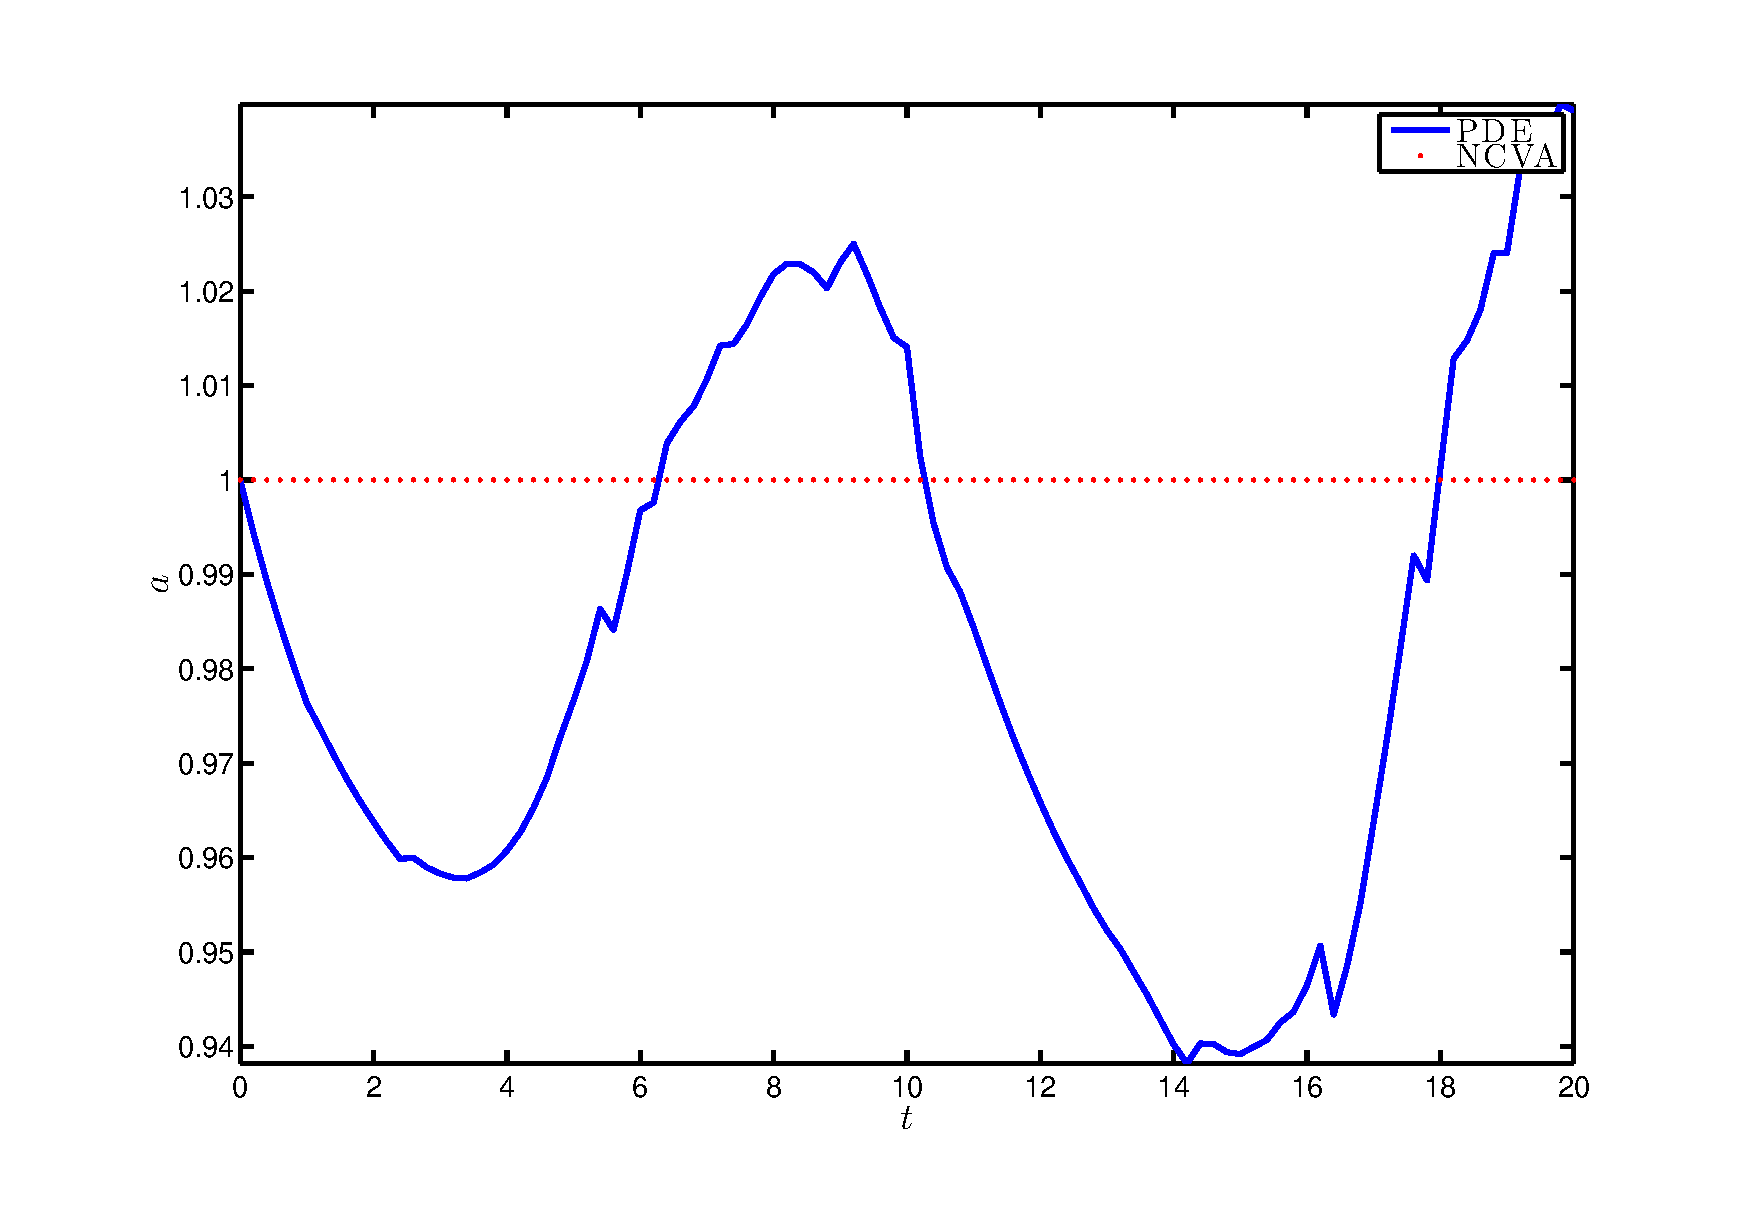
\includegraphics[width=\textwidth, height = \textwidth]{PE01a.eps}
%	         \caption{Amplitude parameter comparison $a(t)$ between PDE and NCVA solutions.}
%	         \label{fig:PLoss01a}
%	     \end{subfigure}
%  \begin{subfigure}[b]{0.5\textwidth}
%  		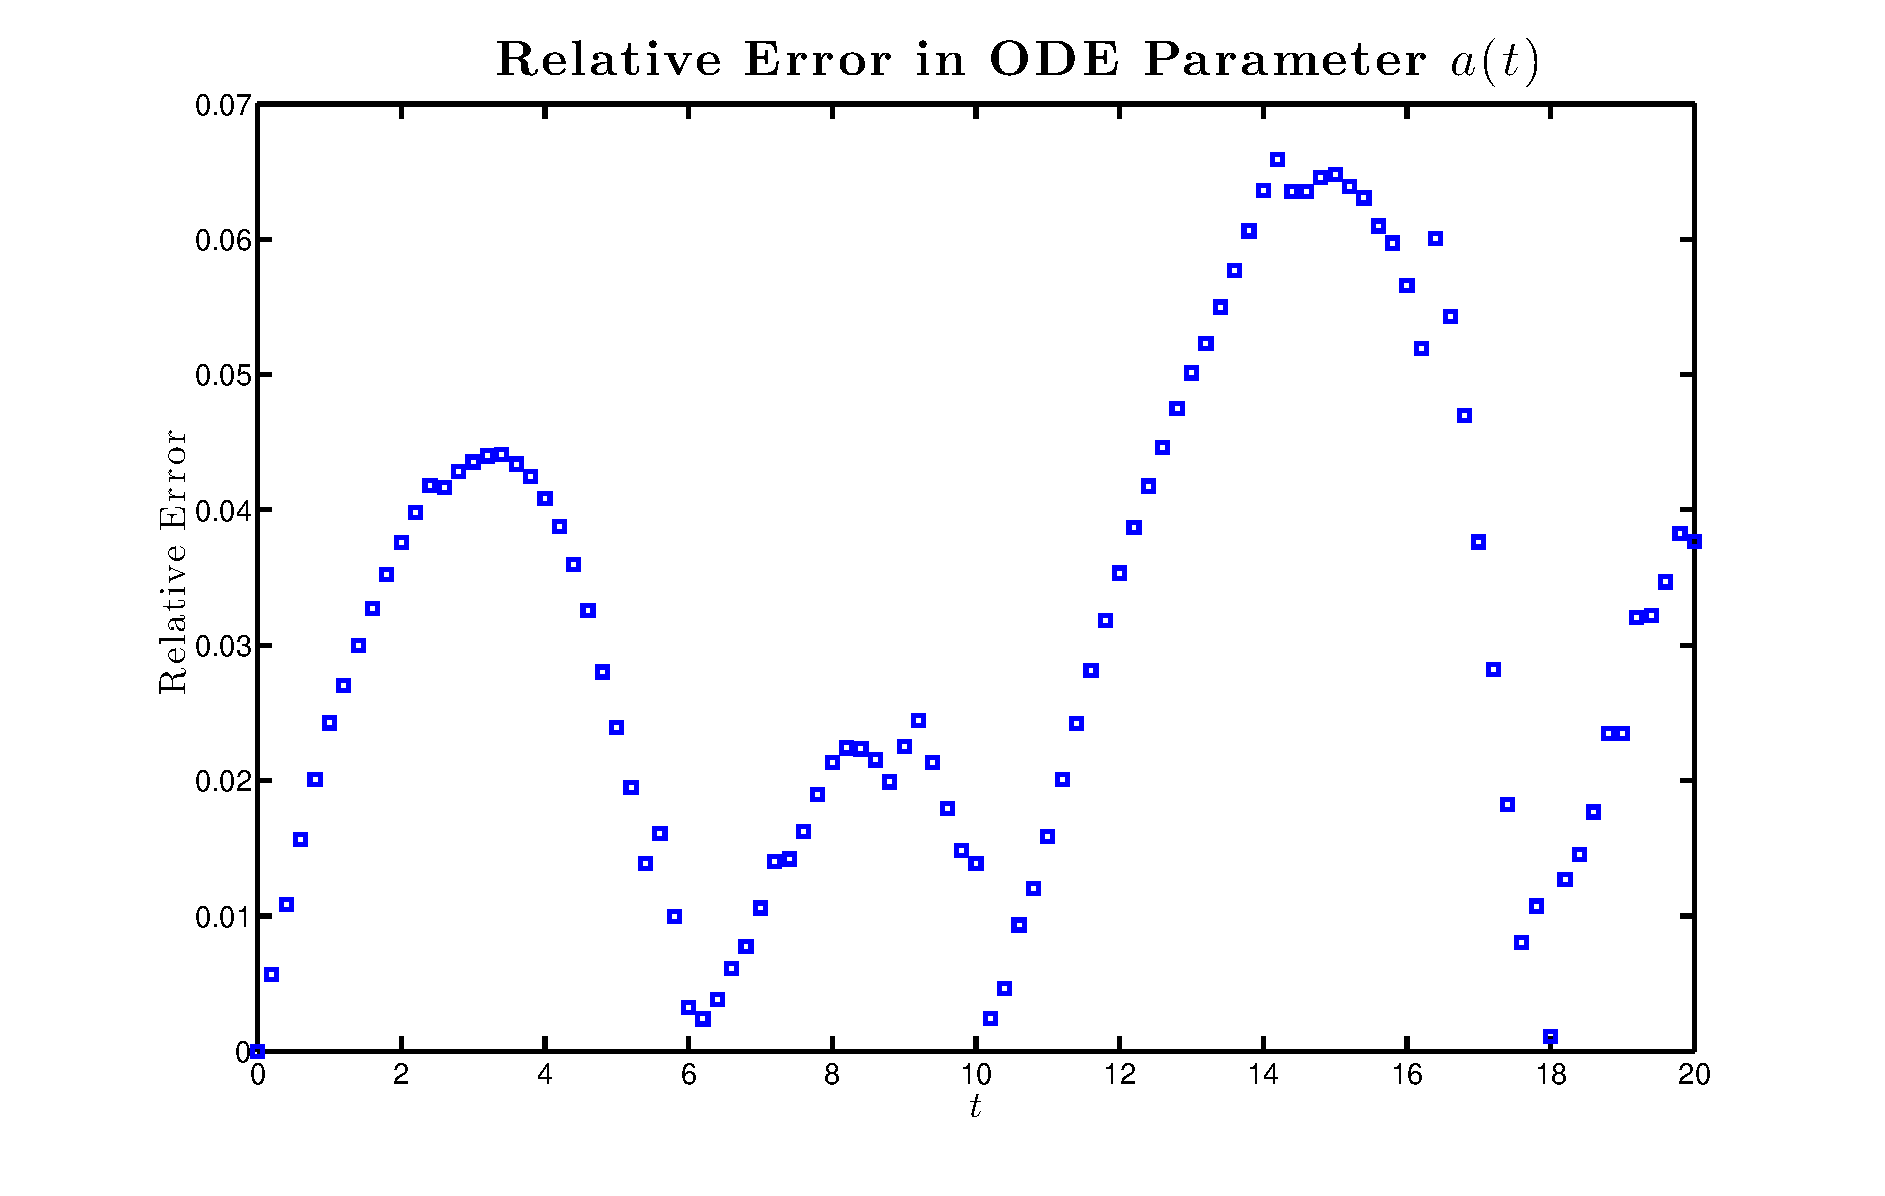
\includegraphics[width= \textwidth, height = \textwidth]{PE01relativeError.eps}  
%	          \caption{Relative error between NCVA and PDE parameter $a(t)$ values.}
%	         \label{fig:PLoss01Err}
%	    \end{subfigure} 
%  \rule{35em}{0.5pt}
%   \caption[Exciton-Polariton Condensate: NLS with Linear Gain $\sigma = 0.1$ and Density Dependent Loss $\chi=(2/3) \sigma$ Amplitude Comparison and Relative Error]{{\bf Exciton-Polariton Condensate:} Amplitude parameter $a(t)$ ansatz comparisons and relative error for  $\chi=2/3 \sigma$ and $\sigma = 0.1$.}
%   \label{fig:PlossA2}
%\end{figure}

\clearpage


\setstretch{1.3}
\chapter{Spontaneous Symmetry Breaking of the Lugiato-Lefever Equation}
\label{chap:LL}
\lhead{Chapter 4. \emph{SSB of the LL Equation}}

\setstretch{2}
The following chapter is based on Ref.~\cite{JuliaSSB} coauthored with Ricardo Carretero-Gonz\'alez, Panayotis G. Kevrekidis, and Mariana Haragus.  The aim of the chapter is to further extend the NCVA approach to a variant of the NLS equation: the mean-field Lugiato-Lefever (LL) 
model~\cite{LL,LLE}.  Experimentally~\cite{XuCoen}, temporal spontaneous symmetry breaking (SSB) is found in passive Kerr resonators described by the LL equation.  We examine this SSB-induced 
instability interval in the the passive 
Kerr resonator modeled by the Lugiato-Lefever equation %Eq.~(\ref{NLSEq})
by means of the NCVA~\cite{JuliaNCVA} described in Chapter~\ref{chap:NCVA}, and further through
a center manifold reduction~\cite{MH-Iooss}
enabling the analysis of the dominant associated eigenmodes (responsible
for determining the spectral stability of the system).  
It is relevant to mention at this point that a thorough  bifurcation analysis for a LL equation in the case of constant external pumping
was recently carried out in Ref.~\cite{LLE_french_PRA}, showing quite complex bifurcation scenarios in both the anomalous and normal dispersion regimes.
%
In the NCVA context, our aim is to
apply a variational method based on well-informed ans\"{a}tze 
in the corresponding
Lagrangian of the system.  The ans\"{a}tze reduce the complexity of the 
original 
infinite-dimensional problem to a few degrees of freedom capturing the 
principal,
static and dynamic characteristics of the system.  
%
This method attempts to project the infinite-dimensional dynamics of the Lugiato-Lefever equation 
%Eq.~\ref{NLSEq} 
into a low-dimensional dynamical system that qualitatively and, to some
extent, quantitatively captures SSB bifurcations an the solutions emanating from it.
%
%However, it is important to note that traditional variational methods rely on the 
%existence of a Lagrangian or Hamiltonian structure for closed systems for which 
%equations of motion can be derived. Nonetheless, recently, 
Based on Galley's~\cite{Galley} approach to extend variational approximation method to open, non-conservative dissipative systems we developed the NCVA,  
which in turn was generalized to dissipative (containing gain and loss) NLS-type
systems in Ref.~\cite{JuliaNCVA}.  This was inspired by the work of Ref.~\cite{ref4} on the 
extension of Galley's formalism to ${\mathcal PT}$-symmetric variants of field theories. It is this variant of the NCVA that we will explore in the present
setting.

The chapter is organized as follows.
%
In Sec.~\ref{section:SSB} we introduce SSB and setup the LL model.  In Sec.~\ref{secModel} we identify the equilibria and study their stability by means 
of a spectral analysis of the linearization problem; this is a perspective
that was absent in the original work of Ref.~\cite{XuCoen} and which, we 
argue, provides a more systematic insight into the stability (and the
potential instabilities) of the system. 
In doing so, we recover the forward and reverse 
pitchfork bifurcations (i.e., a pitchfork loop) observed in Ref.~\cite{XuCoen} as well 
as identify a Hopf bifurcation for larger pump power giving rise to asymmetric,
stable, periodic solutions; the latter is an important feature of 
dynamical interest
in its own right.
%
%Section~\ref{secNCVA} is devoted to the NCVA approach.
%In Sec.~\ref{secNCVA:prelim} we provide a brief description of the 
%NCVA approach and its formulation within the LL model.
%
Section~\ref{secNCVA:app} is devoted to the application of the NCVA to capture
the SSB bifurcation for physically relevant parameters values of the system 
as in Ref.~\cite{XuCoen}.
%
In Sec.~\ref{secGalerkin} we complement our understanding of the pitchfork
loop bifurcation by giving the local bifurcation analysis which is effective 
towards qualitatively and quantitatively describing the emerging asymmetric solutions
close to the pitchfork bifurcation points. 
%
Finally, in Sec.~\ref{secConclusion} we summarize
our findings.
% and we provide possible
%avenues for future research.

\setstretch{1.3}
\section[Spontaneous Time-Reversal Symmetry Breaking in Passive Kerr Resonator]{Spontaneous Time-Reversal Symmetry Breaking in \\
Synchronously-Pumped Passive Kerr Resonators} \label{section:SSB}
\setstretch{2}
%
Spontaneous symmetry breaking (SSB) is the basis for many phase transitions and account for effects including ferromagnetism, superconductivity, and convection cells~\cite{zurek,stanley}.
%
SSB has been widely observed in nonlinear optics and is at the heart of numerous
fundamental phenomena including, but not limited to, asymmetric
dynamics in coupled 
mode models~\cite{kenkre}, optical wave guide arrays~\cite{Boris_Gisin_Kaplan_PRE_2000},
coupled nonlinear micro-cavities~\cite{Haelterman_OE_2006}, 
photonic lattices~\cite{Panos_PLA_2005}. For a detailed exposition
of numerous recent directions within the subject from the perspective
of nonlinear phenomena, see Ref.~\cite{Boris_SSB_book}.
%
SSB is not restricted to Hamiltonian (conservative) systems. For instance, 
over the past few years, it has also played a prominent role in the context of parity-time, 
so-called ${\mathcal PT}$, symmetric
systems~\cite{kivshar,yang} bearing a balanced interplay between 
gain and loss. 
%
There, it is responsible for the emergence 
%and bifurcation of solitons,
%vortices~\cite{rcg:85} and their so-called 
of novel ``ghost'' states both in the case of dimers~\cite{cartarius}, but also in that
of continuous media~\cite{rcg:88}, where they can be responsibility
for the destabilization and bifurcations associated with solitary
waves and vortices.

%in {\cal PT}-symmetric systems containing 
A remarkable example of SSB in a dissipative system was observed by 
Xu and Coen in Ref.~\cite{XuCoen} where a system using an optical fiber ring cavity composed of 
a synchronously-pumped 
passive optical resonator filled with a Kerr nonlinear material was experimentally 
explored. This system exhibits a {\em temporal} SSB instability in which the 
discrete time-reversal symmetry is broken and symmetric states become unstable
in favor of stable asymmetric states.  
%
It is the purpose of the present chapter to complement
the experimental and numerical analysis of Ref.~\cite{XuCoen} by
putting forward a thorough analytical
(and partially numerically assisted) 
understanding of the origin and manifestation of SSB bifurcations in this 
system.

We consider, as in Ref.~\cite{XuCoen}, a model for a passive Kerr resonator in an 
optical fiber ring cavity described by a single PDE,
resulting from an averaging procedure, of the NLS
equation-type, known as the mean-field Lugiato-Lefever (LL) 
model~\cite{LL,LLE}. The LL
equation, taking into account gain and loss in the system, can be cast, 
in non-dimensional form, as~\cite{XuCoen,XuCoenRef22a,XuCoenRef22b}:
%
\begin{equation}
\frac{\partial E(z, \tau)}{\partial z} = \left[ -1 + i (\left\vert E\right\vert^2 - \Delta ) - i \eta \frac{\partial^2}{\partial \tau^2} \right] E + S(\tau), 
\label{NLSEq}
\end{equation}
%
where $z$ is the slow evolution variable of the intracavity field $E$ over 
successive normalized cavity round-trips and $\tau$ describes the temporal 
%profile of 
variable in the dependence of the intracavity pulse envelope.  
%
The terms in the right-hand-side  of Eq.~(\ref{NLSEq}) correspond, respectively, to
cavity losses $(-E)$, Kerr nonlinearity $(i \left\vert E\right\vert^2 E)$, cavity 
phase detuning $(-i \Delta E)$, chromatic dispersion 
$( - i \eta \frac{\partial^2}{\partial \tau^2}E)$, and external pumping $( S(\tau))$.  
%
Within this non-dimensional form~\cite{XuCoenRef22a,XuCoenRef22b}, 
the cavity phase detuning
corresponds to $\Delta = \delta_0\alpha$, where $\alpha$ is half the fraction of 
power lost per round-trip and the cavity finesse is $\mathscr{F} = \pi/\alpha$, and 
$\delta_0 = 2m\pi  - \phi_0$ where $\phi_0$ is the overall cavity round-trip 
phase shift and $m$ is the order of the closest cavity resonance.  
%
The sign of the group-velocity dispersion coefficient of the fiber is $\eta$ 
which is taken as $\eta = -1$ for our analysis with self-focusing nonlinearity.  
The field envelope of the external pump pulses, $S(\tau)$, is modeled by a symmetric chirp-free Gaussian pulse given by $S(\tau) = \sqrt{X} \exp\left[ -(\tau/T_0)^2 \right]$,
with $T_0 = 2.3$ as in the experiments of Ref.~\cite{XuCoen}.

For the SSB instability of the passive Kerr cavity, the pump pulse field profile is temporally symmetric, $S(\tau) = S(-\tau)$, and the model is symmetric under a time reversal transformation, $\tau \rightarrow -\tau$, 
yet it admits asymmetric solutions, as described in Ref.~\cite{XuCoen}.  The 
associated pitchfork bifurcation illustrates that at low pump peak power $X$, the solutions are symmetric in time; however, above a certain pump peak power threshold the symmetric states become unstable while stable asymmetric states
emerge.  
%
The particular experimental parameters of Ref.~\cite{XuCoen} generate, as $X$ is
increased further, a reverse pitchfork as well, in which the asymmetric states
collide and disappear while the symmetric state recovers its stability.
%
%The decline in the observed $|E(\tau=0)|^2$ is caused by the peak of the 
%intracavity pulse shifting towards the right or left and breaking alignment 
%with the center of the pump pulse.
%For $\Delta = 0.92$ and $T_0=2.3$, the bifurcation point for the instability 
%is obtained at $X=4.55$ in Ref.~\cite{XuCoen}.
%
%The main aim of this manuscript is 


%%%%%%%%%% Section Stability
\subsection{The Full Lugiato-Lefever Model: Equilibria, Stability and Bifurcations
\label{secModel}}
%
In this section, we follow the various equilibria of Eq.~(\ref{LugiatoLefever}) as the 
peak pump power, $X$, is varied and determine their stability.  
%
Let us recast Eq.~(\ref{NLSEq}) into the simpler form
%
\begin{equation}
 i u_z + u_{\tau \tau} + (|u|^2 - \Delta) u = - i u  + i S(\tau),
 \label{LugiatoLefever}
\end{equation}
%
which corresponds to the NLS with additional non-conservative terms
(namely the terms in the right-hand side).
%
In what follows, we identify stationary solutions, $u(z,\tau)=u_0(\tau)$
%e^{i \mu z}$, 
of Eq.~(\ref{LugiatoLefever}) by numerically solving the steady-state equation
%
\begin{equation}
 u_{0,\tau \tau} + (|u_0|^2 - \Delta) u_0 = - iu_0  + i S(\tau).
\label{u0}
\end{equation}
% 
It is relevant to mention that since the forcing 
(pump) term in Eq.~(\ref{NLSEq}) is independent
of the field's wavefunction, it is necessary for the steady state to 
be independent of $z$ (i.e., here the detuning parameter $\Delta$ 
plays the role of the frequency). It is also 
worth mentioning that the steady state
is, in general, complex which, as we will see below, is crucial for the steady
state to sustain itself through a stationary flow from the gain to the loss
portions of the solution.  

Let us now consider the stability of the steady state $u_0$ by means 
of a spectral stability analysis.
Specifically, small perturbations of order $\mathcal{O}(\epsilon)$, 
with $0<\epsilon \ll 1$, to the stationary solutions are introduced in the 
form:
%\footnote{Here, again, the perturbation shares the zero frequency of
%the steady state $u_0$.}
%
\begin{equation}
u(z, \tau) =  u_0(\tau) + \epsilon [ a(\tau)e^{\lambda z} + b^*(\tau)e^{\lambda^* z}],
%u(z, \tau) = e^{-i\mu z} \{ u_0(\tau) + \delta [ a(\tau)e^{i\lambda z} + b^*(\tau)e^{-i \lambda^* z}] \},
%\label{BdG}
\nonumber
\end{equation}
%
and substituted into Eq.~(\ref{LugiatoLefever}).  Then, the ensuing linearized equations are solved to $\mathcal{O} (\epsilon)$, leading to the eigenvalue problem:
%
\begin{align}
i \lambda \begin{pmatrix} a(z) \\ b(z) \end{pmatrix} = \begin{pmatrix} M_1 & M_2 \\  -M_2^* & -M_1^* \end{pmatrix} \begin{pmatrix} a(z) \\ b(z) \end{pmatrix}, 
\label{PDEEigenProblem}
\end{align}
%
for the eigenvalues $\lambda$ and associated eigenvector $\xi = (a(z),b(z))^\mathrm{T}$,
where $(\cdot)^*$ denotes complex conjugation and $M_1$ and $M_2$ are the following
operators:
%
\begin{align}
%M_1 &= -\mu - \frac{\partial^2}{\partial \tau^2} - 2|u_0|^2+(i+\Delta), \nonumber \\
M_1 &=  - \partial_\tau^2 - 2|u_0|^2+(\Delta - i), \nonumber \\
M_2 &= -u_0^2.
\end{align}
%
The stationary solutions are linearly unstable provided Re$(\lambda)> 0$.
When unstable, the dynamics of the respective instabilities can be monitored 
through direct numerical simulations of Eq.~(\ref{LugiatoLefever}).
%
It is relevant to mention at this point that a thorough (Turing) stability analysis 
for frequency combs in both the anomalous and normal dispersion regimes
was recently carried out in Ref.~\cite{LLE_french_PRA}.

%%%%%%%%%% Fig 1 %%%%%%%%%%%%%%%%%%%%%%%%%%%%%%%%%
\begin{figure}[htb!]
\centering
\centerline{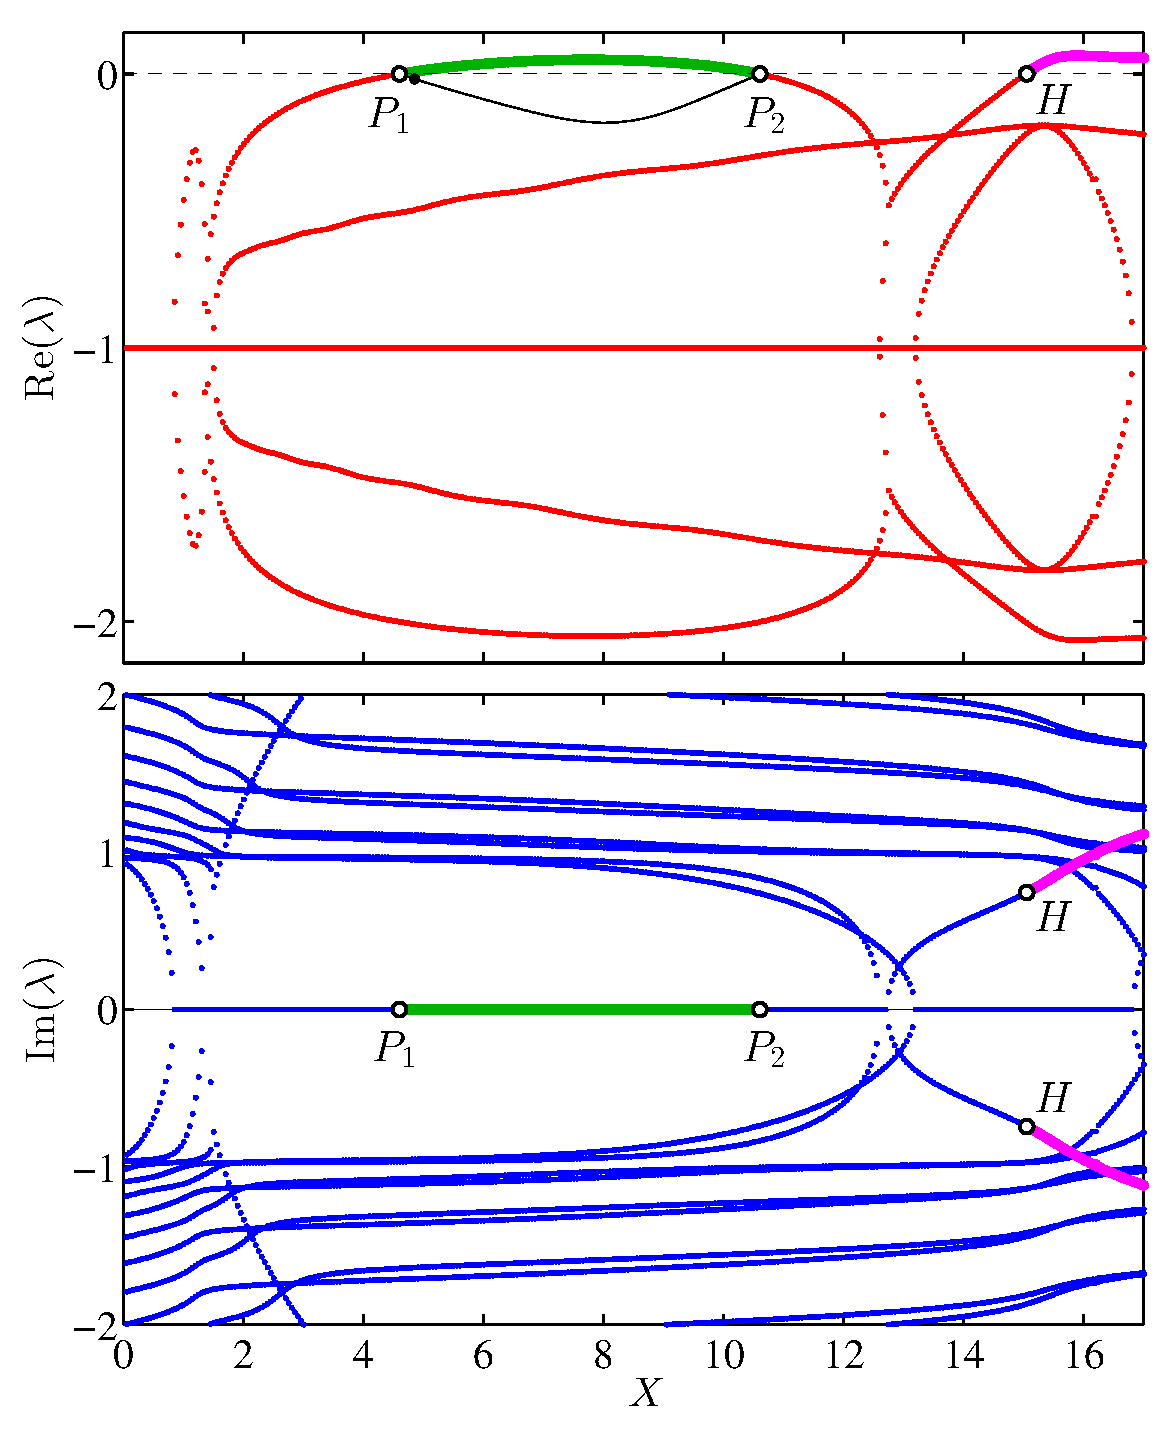
\includegraphics[width=0.9\textwidth]{frequencySpectrumNN.eps}}
  \rule{35em}{0.5pt}
\caption[LL Equation Linearization Spectrum for the Symmetric and Asymmetric 
Steady State Solutions]{Linearization spectrum for the symmetric and asymmetric 
steady state solutions of 
the Lugiato-Lefever equation (\ref{LugiatoLefever})
as the pump power $X$ is varied for $\Delta = 0.92$ and $T_0=2.3$.  
The top and bottom panels depict, respectively, the real and imaginary
parts of the eigenvalues.
%
Stable symmetric solutions bearing Re$(\lambda)<0$ are depicted by 
small (red) dots in the top panel while unstable symmetric solutions 
are depicted with thick solid lines.
%
The thick (green) solid line between the points $P_1$ and $P_2$ represents
the unstable solutions through a forward ($P_1$) and reverse ($P_2$)
pitchfork bifurcations.
%
The thin (black) curve between the points $P_1$ and $P_2$ corresponds to the 
stable asymmetric solution branches created through the pitchfork bifurcation.
(The small black dot next to the point $P_1$ is the stable eigenvalue
used for the slope computation in Fig.~\ref{PitchPhasePortrait}.)
%
The thick (magenta) solid line to the right of the Hopf bifurcation point
$H$ indicates the onset of instability for the symmetric state and the 
existence of an asymmetric periodic solution.
%
}
\label{fig:frequencySpectrum}
\end{figure}
%%%%%%%%%% Fig 1 %%%%%%%%%%%%%%%%%%%%%%%%%%%%%%%%%


Figure~\ref{fig:frequencySpectrum} depicts the linearization 
spectrum for the symmetric stationary
solution [see (red) dashed line in panels (c) and (d) of Fig.~\ref{fig:evolution}] 
as a function of the pump peak power.  
%
The spectrum in Fig.~\ref{fig:frequencySpectrum} evidences the existence of two 
unstable branches:
%
(i) a pitchfork bifurcation loop containing a forward pitchfork 
bifurcation, see point $P_1$ at $X\approx 4.6$, and a reverse pitchfork
bifurcation, see point $P_2$ at $X\approx 10.6$, and 
%
(ii) a Hopf bifurcation, see point $H$ at $X\approx 15.1$.
%
The pitchfork bifurcation, see thick (green) line between the 
points $P_1$ and $P_2$ in Fig.~\ref{fig:frequencySpectrum}, 
is responsible, as the pump power is increased, for the loss of stability of the 
symmetric state towards a pair of asymmetric states (one to the left and one to the 
right) at $P_1$. As the pump power is increased, a reverse pitchfork at $P_2$
is responsible for the collision (and annihilation) of the two asymmetric states 
towards the symmetric state that recovers its stability.
%
A sample of the dynamic destabilization of the (unstable) symmetric state
for a pump strength $X=8$, namely between the two pitchfork points, is depicted 
in Fig.~\ref{fig:evolution}(a). As the figure shows, the symmetric state 
[see dashed (red) line in Fig.~\ref{fig:evolution}(c)] destabilizes
towards the stable, asymmetric state [see solid (blue) line in
Fig.~\ref{fig:evolution}(c)].
%
On the other hand, the instability due to the Hopf bifurcation branch,
see the thick (magenta) line emanating from the point $H$ in
Fig.~\ref{fig:frequencySpectrum}, is responsible for the instability of
the symmetric state towards a {\em periodic} (in $z$) solution. A sample of the
evolution for the symmetric state towards the stable periodic solution
is depicted in Fig.~\ref{fig:evolution}(b). The periodic solution contains
three ``humps'' in its $\tau$ dependence: 
a central one performing left-to-right oscillations while
the side ``humps'' oscillate alternatively up-and-down. Snapshots for the
asymmetric states when the side ``humps'' have the largest magnitude are
depicted in panel (d) corresponding to the times depicted by horizontal
white lines in panel (b).

%%%%%%%%%% Fig 2 %%%%%%%%%%%%%%%%%%%%%%%%%%%%%%%%%%%%%%%%%%%%%%%%
\begin{figure}[t]
\centering
\centerline{
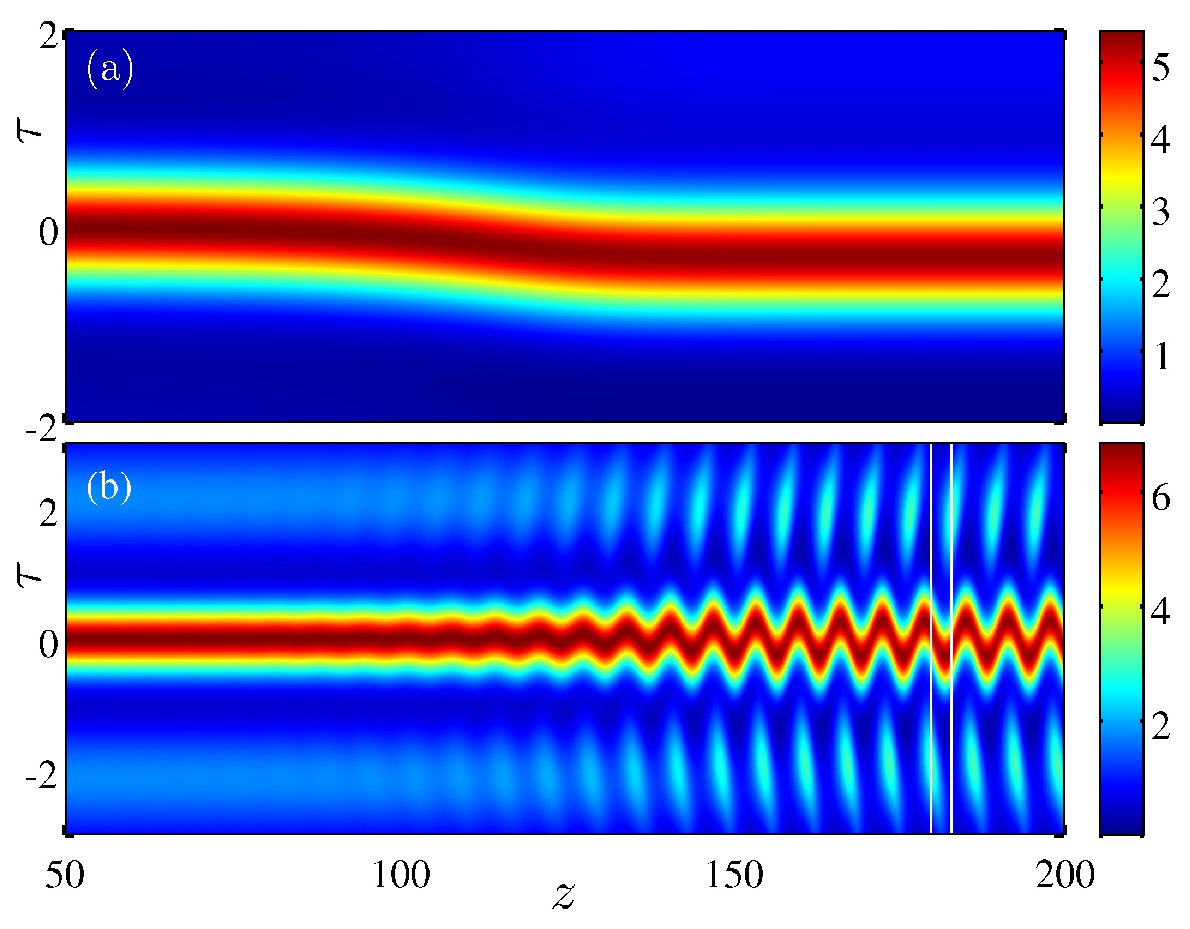
\includegraphics[width=0.85\textwidth]{densityX8X16_t.eps}}
\centerline{ 
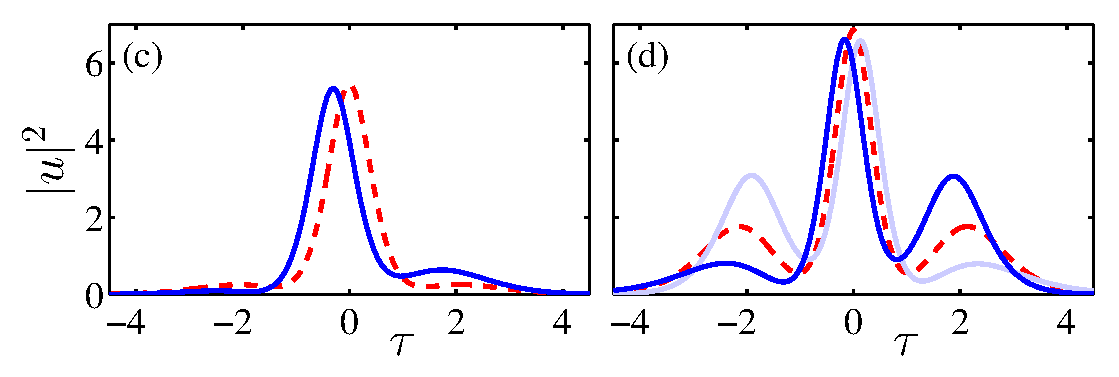
\includegraphics[width=0.85\textwidth]{snaps_X8_X16.eps}
\vspace{-0.3cm}
}
  \rule{35em}{0.5pt}
\caption[Density Evolution of Unstable Symmetric States at $X=8$ and 16 and Snapshots]{
(a), (b) Examples for the density evolution of unstable symmetric states
and 
(c), (d) snapshots for the corresponding states.
%
(a) Evolution of unstable symmetric state for $X=8$ between the two pitchfork bifurcations 
$P_1$ and $P_2$ depicted in Fig.~\ref{fig:frequencySpectrum}. The initial symmetric state,
see dashed (red) line in panel (c) evolves towards the asymmetric steady state
depicted in solid (blue) in panel (c).
%
(b) Evolution of unstable symmetric state towards a periodic breathing solution
for $X=16$ (i.e., to the right of the Hopf bifurcation point $H$ in 
Fig.~\ref{fig:frequencySpectrum}). The initial symmetric state [dashed (red)
line] and two snapshots of the density for the periodic solution [solid (blue and 
light blue) lines] separated by half a period, at the times corresponding to the white
vertical lines in panel (b), are depicted in panel (d).
\label{fig:evolution}}
\end{figure}
%%%%%%%%%% Fig 2 %%%%%%%%%%%%%%%%%%%%%%%%%%%%%%%%%%%%%%%%%%%%%%%%

It is important to mention that, due to the cavity loss term ($-iu$), the
real part of the spectrum is symmetric with respect to Re$(\lambda)=-1$
(see Sec.~\ref{secGalerkin} for details).
Therefore, tuning the cavity loss parameter is crucial to the existence of the
SSB bifurcation as higher values of this parameter shift the real part of the
spectrum down precluding the possibility of eigenvalues crossing the
origin and leading to such bifurcations. By the same token, reducing the value
of the cavity loss parameter will induce more eigenvalues to cross the
origin and thus lead to richer and more complicated bifurcation scenarios.
A detailed analysis of the bifurcations as the cavity loss parameter is
varied is outside of the scope of the present dissertation work and will be
studied in a future work.

\clearpage
\JMR{\subsection{Numerical Convergence of the Stability Spectrum}}
\label{secEigs}
\JMR{The purpose of this subsection is to briefly discuss the numerics used for analyzing the frequency spectrum (see Fig.~\ref{fig:frequencySpectrum}) which are dependent on the discretization of fast-time $h = d\tau$, the domain length $L$, and the boundary condition.  The eigenvalue problem Eq.~(\ref{PDEEigenProblem}) can be recast as $i\lambda \vec{\xi}  = M \vec{\xi}$.  This is numerically solved using second-order central differencing in one dimension for the Laplacian given by 
\begin{align}
\nabla^2 u_j = \frac{\partial^2 u}{\partial \tau^2}\bigg|_j \approx \frac{u_{j+1} - 2u_j + u_{j-1}}{h^2},
\end{align}
%
and when implemented into the $M_1$ matrix, yields a matrix $A$ which is tridiagonal except from the matrix elements corresponding to the boundary conditions.  Since boundary conditions of the fast-time differencing in a PDE like the LL model have the potential to alter the stability, it is necessary to compare the stability for each of the specific boundary conditions we would like to use.  For this discussion we limit ourselves to three boundary conditions~\cite{LeVeque}:  Dirichlet, Neumann, and periodic.}

\JMR{In our analysis, we consider a uniform grid with spacing $h$ on the interval $[-L/2, L/2]$.  Dirichlet boundary conditions specify a fixed constant value along the boundary of the domain.  For our Dirichlet boundary conditions we define $u(-L/2) = u(L/2) = 0$ given that the solution has the form of a bright soliton.  Using such a formulation the Laplacian matrix with these Dirichlet boundary conditions becomes
\begin{align}
A  = \frac{1}{h^2} \begin{bmatrix} -2 & 1 &  0  &  \cdots  & 0 \\ 1 & -2 & 1  &  \cdots & 0 \\
0 & \ddots & \ddots & \ddots &  0 \\
0 & 0 & 1& -2 & 1 \\
0 & \cdots & 0 & 1 & -2
  \end{bmatrix}.
\end{align} 
%
Neumann boundary conditions specify the value of the derivative of a solution at the boundary of the domain.  We use a no flux boundary in which $\partial_\tau u(-L/2)= \partial_\tau u(L/2) =0$ such that the Laplacian matrix becomes
\begin{align}
A  = \frac{1}{h^2} \begin{bmatrix} -2 & 2 &  0  &  \cdots  & 0 \\ 1 & -2 & 1  &  \cdots & 0 \\
0 & \ddots & \ddots & \ddots &  0 \\
0 & 0 & 1& -2 & 1 \\
0 & \cdots & 0 & 2 & -2
  \end{bmatrix}.
\end{align}
%
The periodic boundary condition is defined as $u(-L/2) = u(L/2)$ and is justified in the scenario of a ring cavity.  The discretized Laplacian matrix for periodic boundary conditions is
\begin{align}
A  = \frac{1}{h^2} \begin{bmatrix} -2 & 1 &  0  &  \cdots  & 1 \\ 1 & -2 & 1  &  \cdots & 0 \\
0 & \ddots & \ddots & \ddots &  0 \\
0 & 0 & 1& -2 & 1 \\
1 & \cdots & 0 & 1 & -2
  \end{bmatrix}.
\end{align}}
%
\JMR{In order to quantify the convergence of the eigenvalues for $h=0.01$, 0.05, 0.1 and 0.5 given $L=10$, 20, 50, 100, and 200 we analyze the spectrum and the Euclidean norm of matrix $M$ for the symmetric state at $X=8$ which is unstable.  If we consider the 2-norm, then we can show the  convergence by explicitly computing the eigenvectors and eigenvalues of the matrix $M$ in Eq.~(\ref{PDEEigenProblem}) [$i\lambda \vec{\xi}  = M \vec{\xi}$].  Since the matrix $M$ from Eq.~(\ref{PDEEigenProblem}) is symmetric, the 2-norm of $M$ is equal to its spectral radius ($\rho(M)$):
\begin{align}
\lvert \lvert M\lvert \lvert_2 = \rho(M) = \max_{1 \le p \le N} \lvert \lambda_p \lvert,
\end{align} 
where $\lambda_p$ is the $p$th eigenvalue of the matrix~\cite{LeVeque}.  Therefore, we will use the spectral radius to give insight into the convergence between the different boundary conditions.  Table~\ref{dxsmall} compares the spectral radius with various domain lengths $L$ and discretization $h$ for the Dirichlet, Neumann, and periodic boundary conditions.  From Table~\ref{dxsmall} we find a small spectral radius for $h=0.5$ ($\rho(M) \approx 17$) when compared to the $h=0.01$ ($\rho(M) \approx 1,600$), which gives an upper bound to the spectral radius.  Therefore, $h=0.5$ is too coarse a grid size with a small spectral radius which does not accurately capture the true eigenvalues.  %Table~\ref{dxsmall} depicts spectral radius of all three boundary conditions for domain lengths greater than $L=10$.  
The spectral radius alone does not explicitly define if the solutions converge to the true eigenvalues.  Therefore, we will also compare the unstable eigenvalue for this system as a measure of convergence between the different boundary conditions.  Table~\ref{unstableeigTable} compares the unstable eigenvalue for various domain lengths $L$ and discretization $h$ for Dirichlet, Neumann, and periodic boundary conditions.  We omit $h=0.5$ since this discretization is too coarse and does not converge to a single unstable eigenvalue for all boundary conditions.  From Table~\ref{unstableeigTable}, we find the largest descretization for convergence of the unstable eigenvalue is $h=0.1$. }

\JMR{\begin{table}[htb!]
\centering
\ra{1.3}
\begin{tabular}{@{}lllllll@{}}\toprule
&& \multicolumn{5}{c}{Domain Length $L$}  \\
\cmidrule{3-7}
&& $10$ & $20$ & $50$ & $100$ & $200$ \\ \midrule
$h = 0.01$ && $N= 1001$ & $N = 2001$ & & & \\ %$N = 5001$ &  & \\ %$N = 10000$ & $N = 20000$ \\
Dirichlet &&    1.6003$\times10^3$ &  1.6008$\times10^3$ & & & \\ 
Neumann && 1.6003$\times10^3$ & 1.6008$\times10^3$ & & & \\ 
Periodic && 1.6007$\times10^3$ & 1.6009$\times10^3$ & & & \\ \midrule
$h = 0.05$ && $N= 201$ & $N = 401$ & $N = 1401$ & $N = 2001$ & \\ % $N = 4001$ \\
Dirichlet && 1.6003$\times10^3$ &1.6008$\times10^3$ & 1.6009$\times10^3$ & 1.6009$\times10^3$ & \\ 
Neumann && 1.6135$\times10^3$ & 1.6136$\times10^3$ & 1.6136$\times10^3$ &1.6136$\times10^3$ & \\ 
Periodic && 1.6007$\times10^3$ & 1.6009$\times10^3$ & 1.6009$\times10^3$ & 1.6009$\times10^3$ & \\ \midrule
$h = 0.1$ && $N= 101$ & $N = 201$ & $N = 501$ & $N = 1001$ & $N = 2001$ \\
Dirichlet && 400.2982 &400.7857  & 400.9032 & 400.9170 & 400.9202 \\ 
Neumann && 404.0546 & 404.0741 & 404.0741 & 404.0741& 404.0741 \\ 
Periodic &&  400.7203 & 400.8860 & 400.9167 & 400.9202 & 400.9210 \\  \midrule
$h = 0.5$ && $N= 21$ & $N = 41$ & $N = 101$ & $N = 201$ & $N = 401$ \\
Dirichlet &&  16.4045 & 16.8224 &  16.9319 & 16.9454 & 16.9485\\ 
Neumann && 16.9710 & 17.0662 & 17.0682 & 17.0682 & 17.0682 \\ 
Periodic && 16.7560 & 16.9149 & 16.9450 & 16.9485 & 16.9493\\ 
\bottomrule
\end{tabular}
\caption[Comparison of the Spectral Radius for Dirichlet, Neumann, and Periodic Boundary Conditions]{Comparison of the spectral radius for Dirichlet, Neumann, and periodic boundary conditions. For discretization size $h = 0.01$, we used two domain lengths $L = 10$ and 20 corresponding to Laplacian matrix size of $N\times N$ .  Given $h=0.5$ four domain lengths $L = 10$, 20, 50, and 100 are compared between the three boundary conditions.  For $h=0.1$ and 0.5 five domain lengths $L = 10$, 20, 50, 100 and 200 are compared.  The spectral radius for $h=0.5$ is too coarse a discretization and fails to converge to the proper eigenvalues.}%The spectral radius for $h=0.5$ does not converge.}
\label{dxsmall}
\end{table}}

\begin{landscape}
\begin{table}[htb!] 
\centering
\ra{1.3}
\begin{tabular}{@{}lllllll@{}}\toprule
&& \multicolumn{5}{c}{Domain Length $L$}  \\
\cmidrule{3-7}
&& $10$ & $20$ & $50$ & $100$ & $200$ \\ \midrule
$h = 0.01$ && $N= 1001$ & $N = 2001$ & & & \\ %$N = 5001$ &  & \\ %$N = 10000$ & $N = 20000$ \\
Dirichlet && 0.052680703192848 & 0.051828350475447 & & & \\ 
Neumann && 0.053646211533514 &  0.051828322918270 & & & \\ 
Periodic && 0.052679254860875 & 0.051828350684082 & & & \\ \midrule
$h = 0.05$ && $N= 201$ & $N = 401$ & $N = 1401$ & $N = 2001$ & \\ % $N = 4001$ \\
Dirichlet && 0.052671286287013 & 0.051840500243317 & 0.051840521421259 & 0.051840521421264 & \\ 
Neumann && 0.053622508462011 & 0.051840474228158 & 0.051840521421259 & 0.051840521421258 &\\ 
Periodic && 0.052663061760651 & 0.051840501211644 & 0.051840521421264 & 0.051840521421259 & \\ \midrule
$h = 0.1$ && $N= 101$ & $N = 201$ & $N = 501$ & $N = 1001$ & $N = 2001$ \\
Dirichlet && 0.052689738246259 & 0.051881121063754 & 0.051881142017631 & 0.051881142017632 & 0.051881142017631 \\ 
Neumann && 0.053620924363313 &  0.051881096702647 &  0.051881142017629 & 0.051881142017633 & 0.051881142017632 \\ 
Periodic && 0.052671246337099 & 0.051881122829374 & 0.051881142017631 & 0.051881142017631 & 0.051881142017633\\  \midrule
\bottomrule
\end{tabular}
\caption[Comparison of Unstable Eigenvalue for Dirichlet, Neumann, and Periodic Boundary Conditions]{Comparison of unstable eigenvalue for Dirichlet, Neumann, and periodic boundary conditions.  The layout is the same as Table~\ref{dxsmall}.  The discretization $h=0.5$ is omitted because it fails to converge to a single unstable eigenvalue.  The largest discretization to use for convergence is $h=0.1$.}
\label{unstableeigTable}
\end{table}
\end{landscape}

\JMR{\begin{figure}[htb!]
\centering
\centerline{
\begin{subfigure}{0.5\textwidth}
\hspace{0.5cm}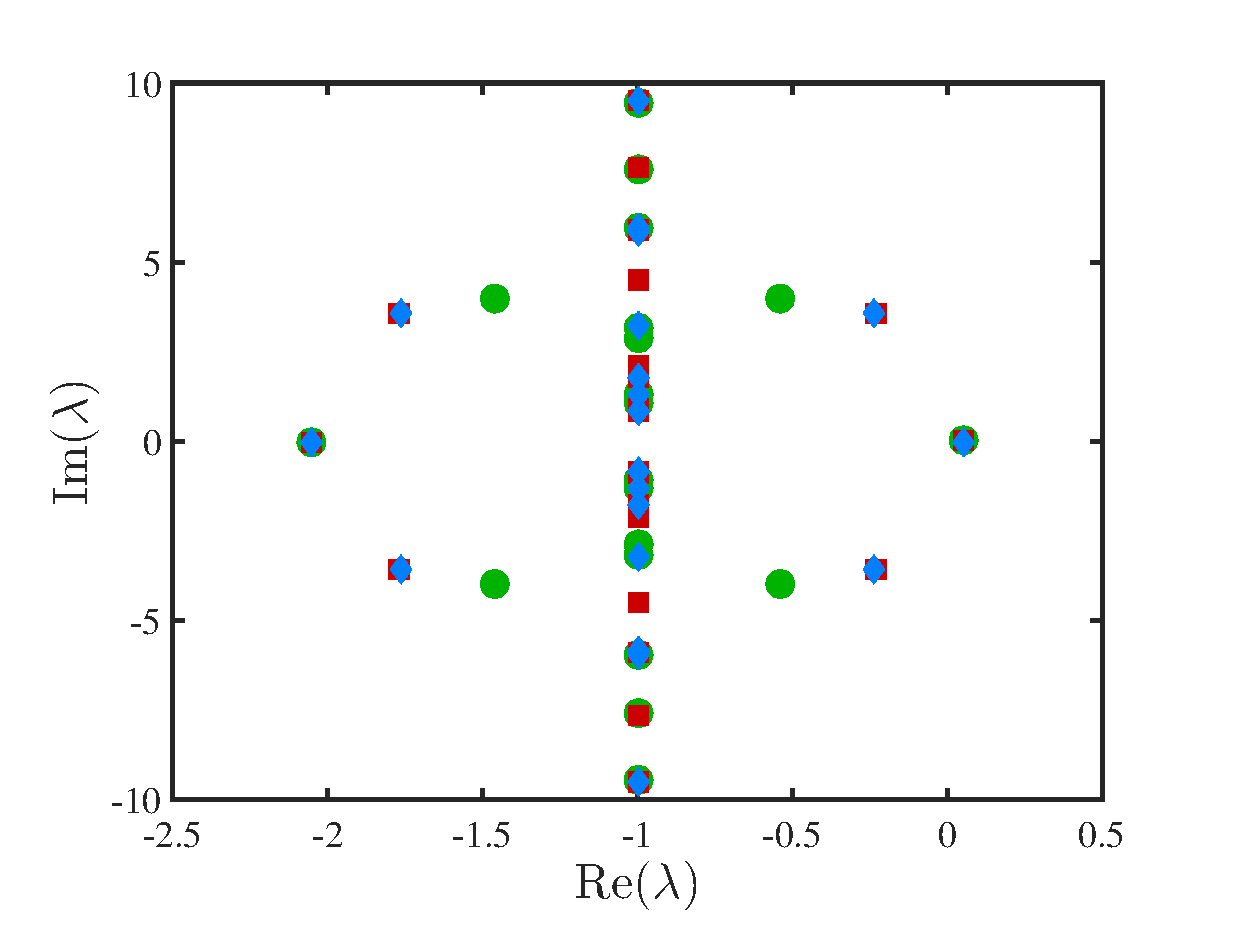
\includegraphics[width=0.9\linewidth]{EigPlot_1.eps}
\caption{$h = 0.01$ }
\end{subfigure}
\begin{subfigure}{0.5\textwidth}
\hspace{0.5cm}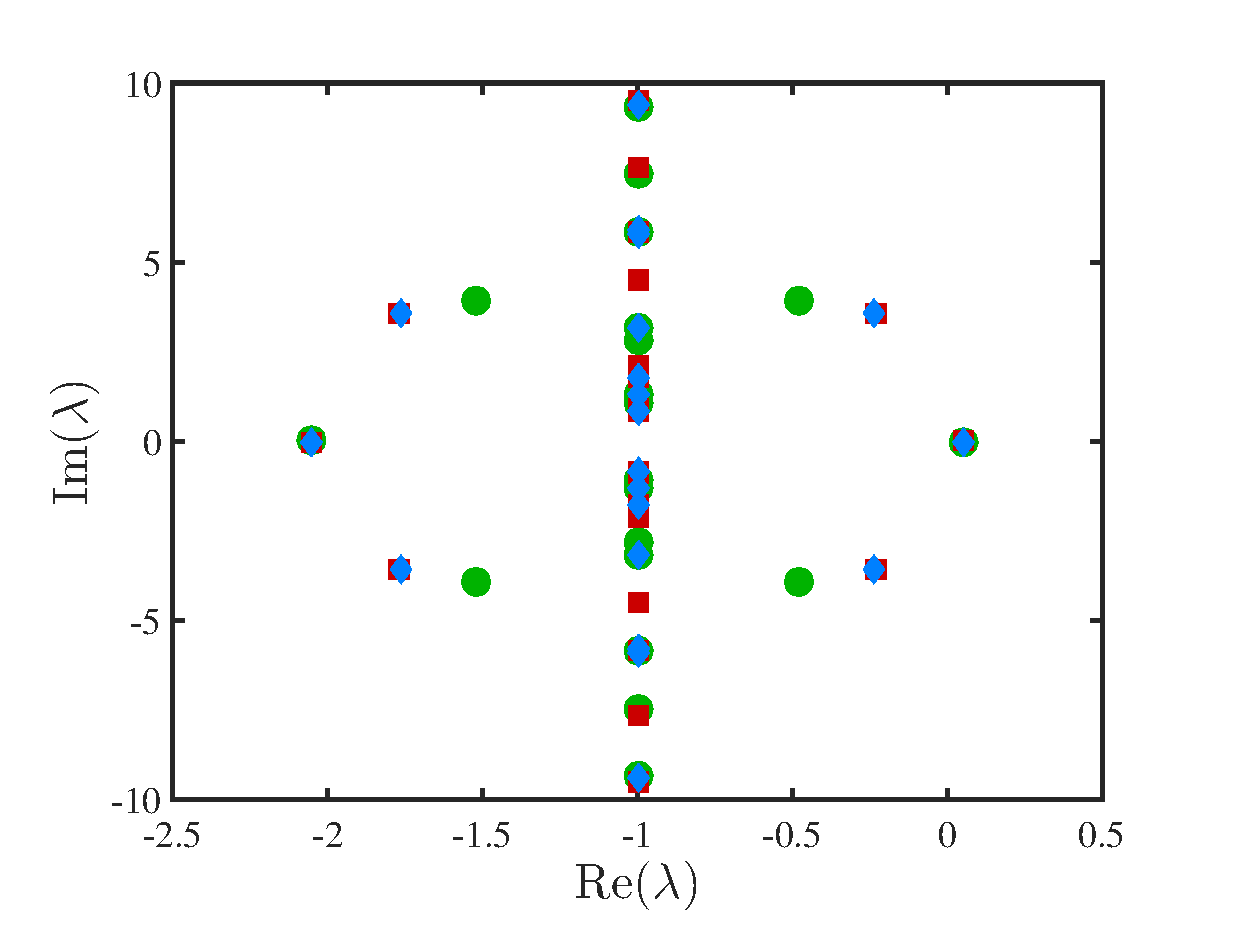
\includegraphics[width=0.9\linewidth]{EigPlot_3.eps}
\caption{$h = 0.05$ }
\end{subfigure}}
\centerline{
\begin{subfigure}{0.5\textwidth}
\hspace{0.5cm}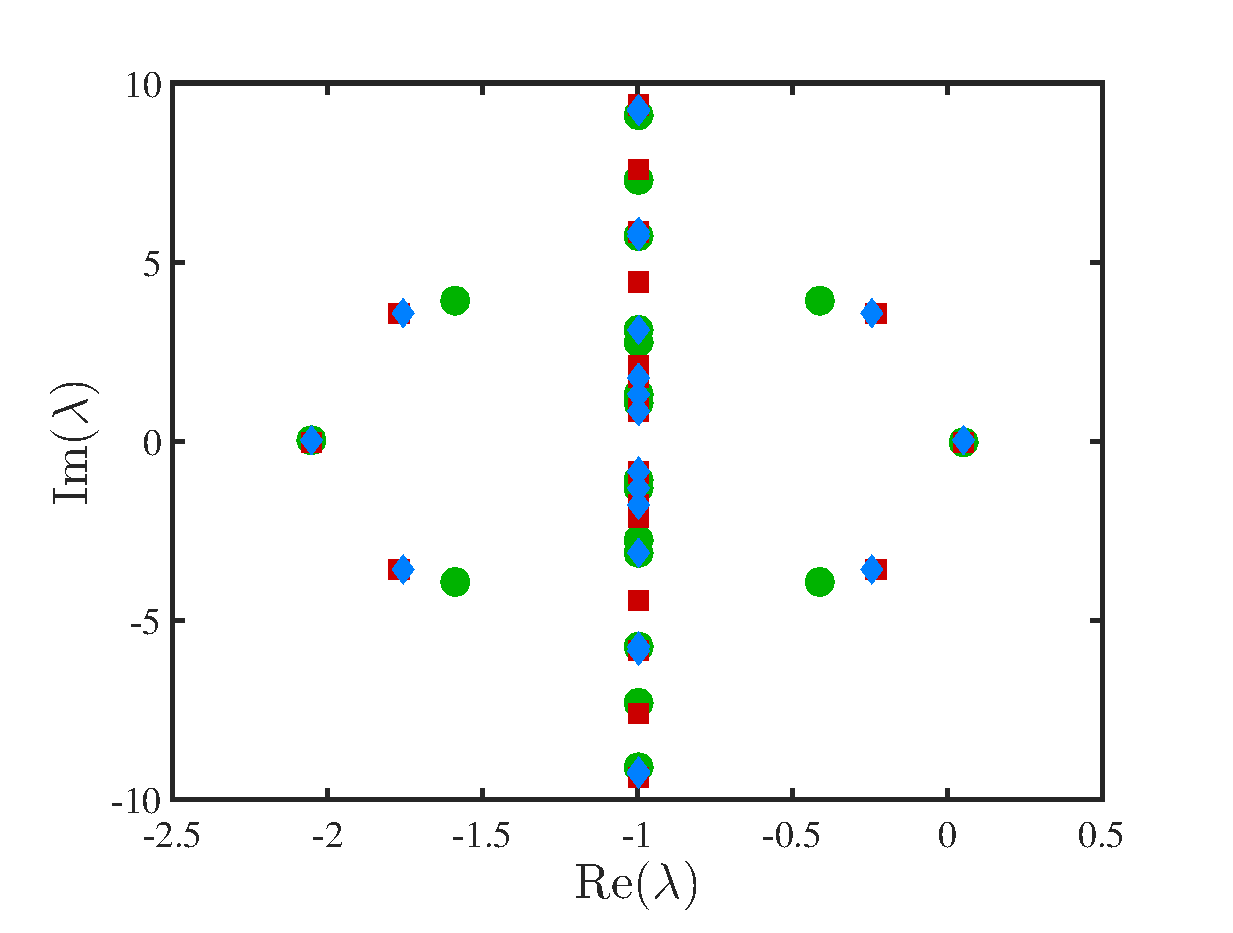
\includegraphics[width=0.9\linewidth]{EigPlot_7.eps}
\caption{$h = 0.1$ }
\end{subfigure}
\begin{subfigure}{0.5\textwidth}
\hspace{0.5cm}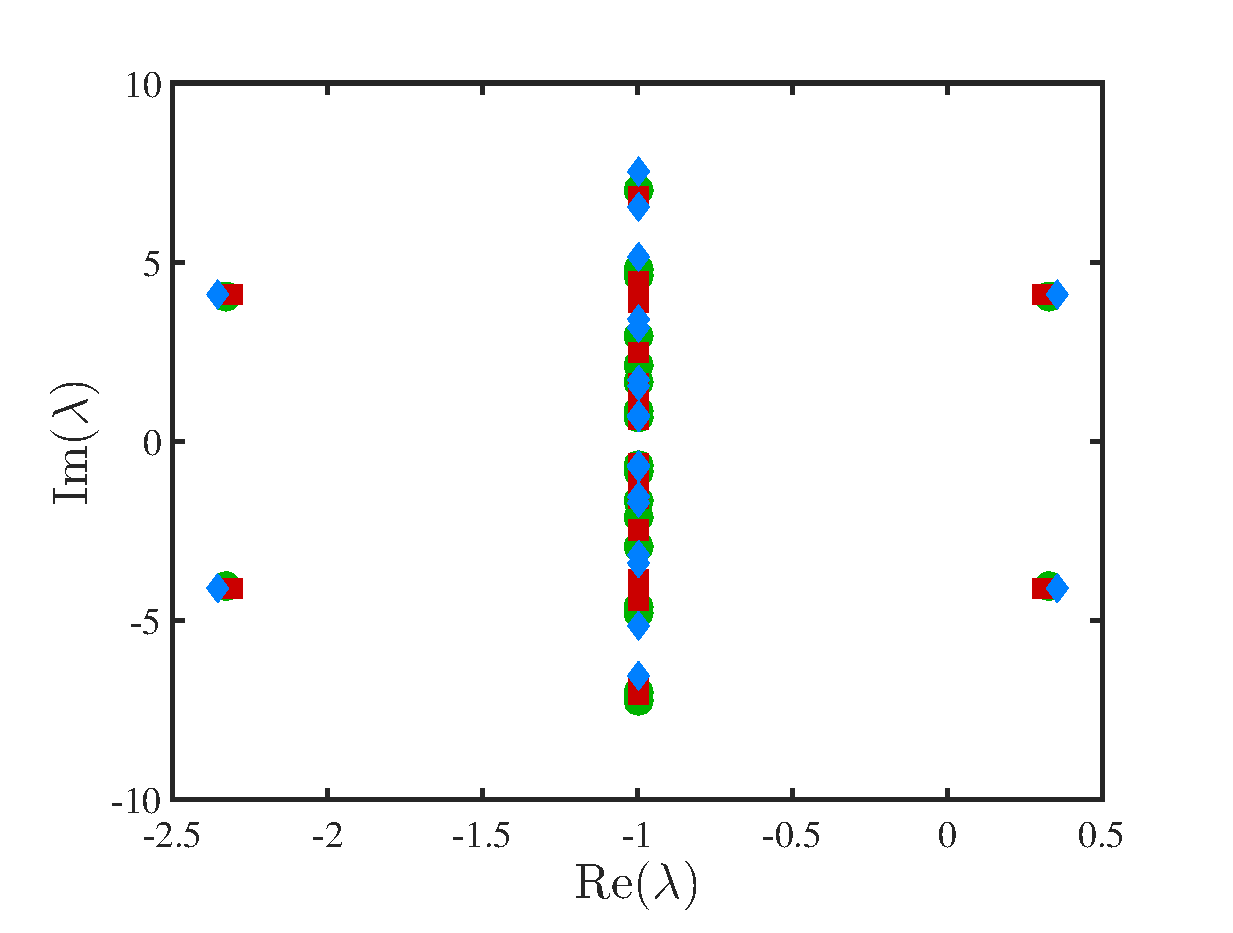
\includegraphics[width=0.9\linewidth]{EigPlot_12.eps}
\caption{$h = 0.5$ }
\end{subfigure}}
  \rule{35em}{0.5pt}
\caption[Comparison of Frequency Spectrum for Domain Length $L$=10]{Comparison of the frequency spectrum for the domain length $L=10$ for (a) $h=0.01$, (b) $h=0.05$, (c) $h=0.1$, and (d) $h=0.5$.  Each plot depicts the frequency spectrums for Dirchlet (green), Neumann (red), and periodic (blue) boundary conditions.  The discretization (d) $h=0.5$ is too coarse and does not converge. }
\label{figAdd1}
\end{figure}
}

\JMR{\begin{figure}[htb!]
\centering
\centerline{
\begin{subfigure}{0.5\textwidth}
\hspace{0.5cm}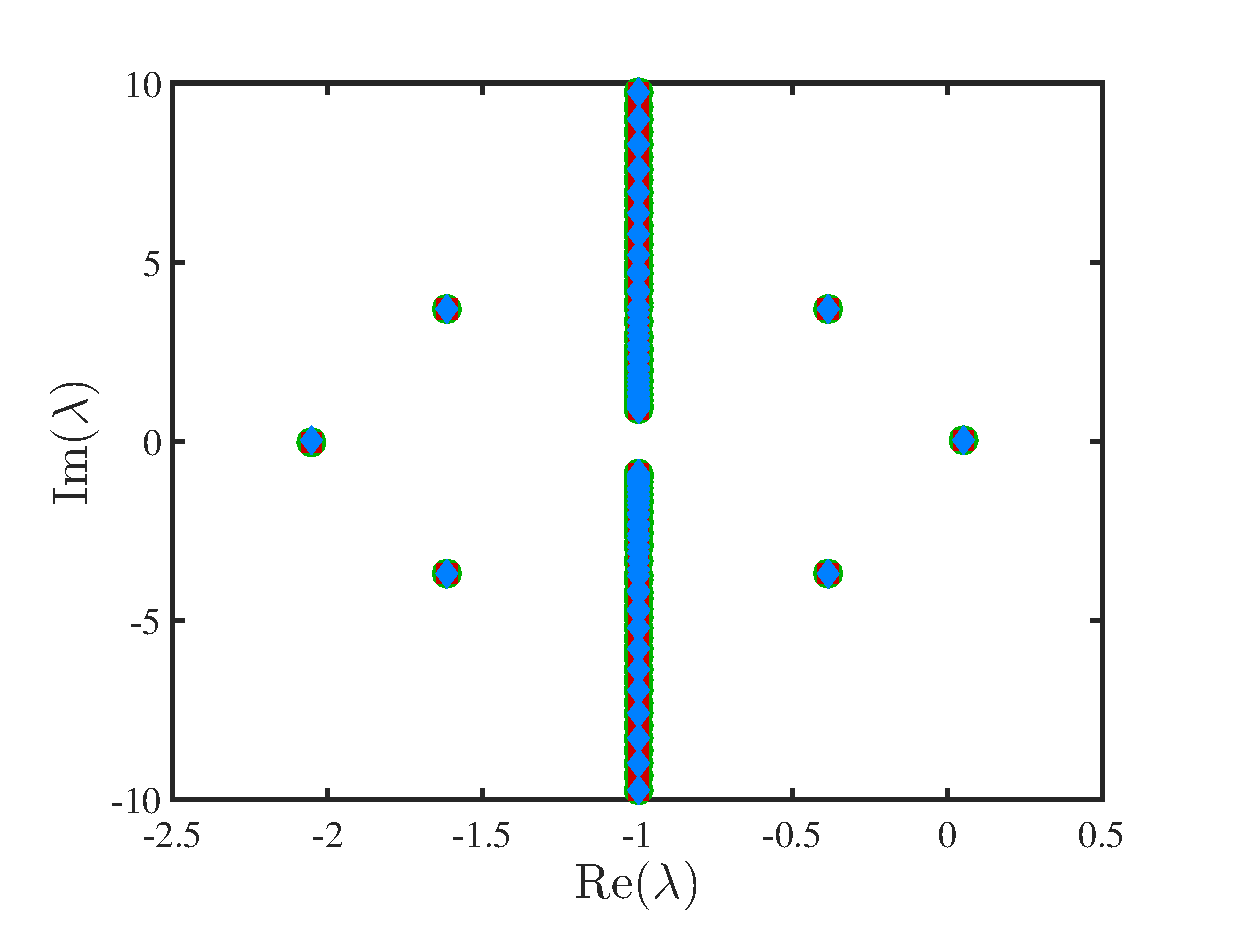
\includegraphics[width=0.9\linewidth]{EigPlot_5.eps}
\caption{$h = 0.05$ }
\end{subfigure}
\begin{subfigure}{0.5\textwidth}
\hspace{0.5cm}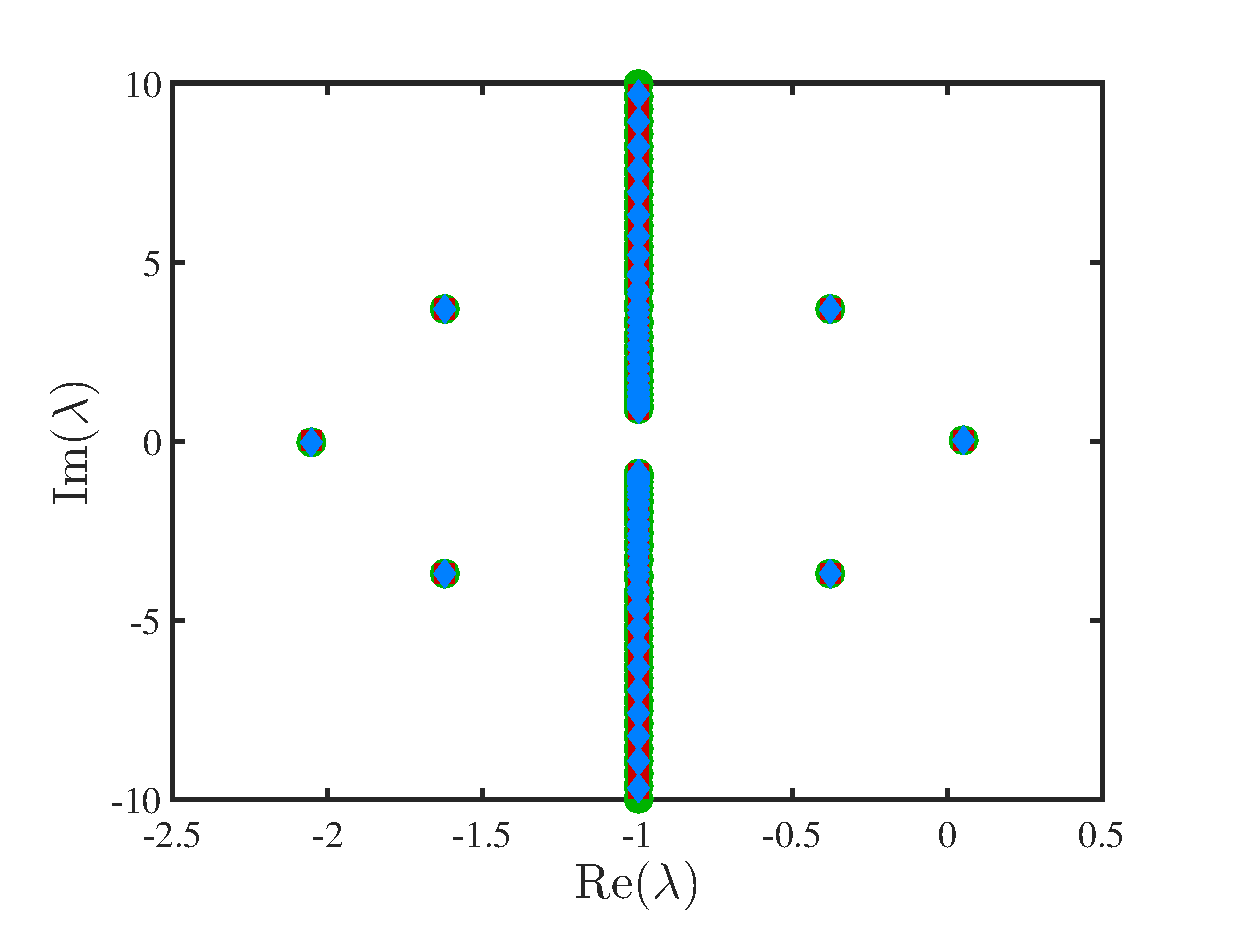
\includegraphics[width=0.9\linewidth]{EigPlot_9.eps}
\caption{$h = 0.1$ }
\end{subfigure}}
\centerline{
\begin{subfigure}{0.5\textwidth}
\hspace{0.5cm}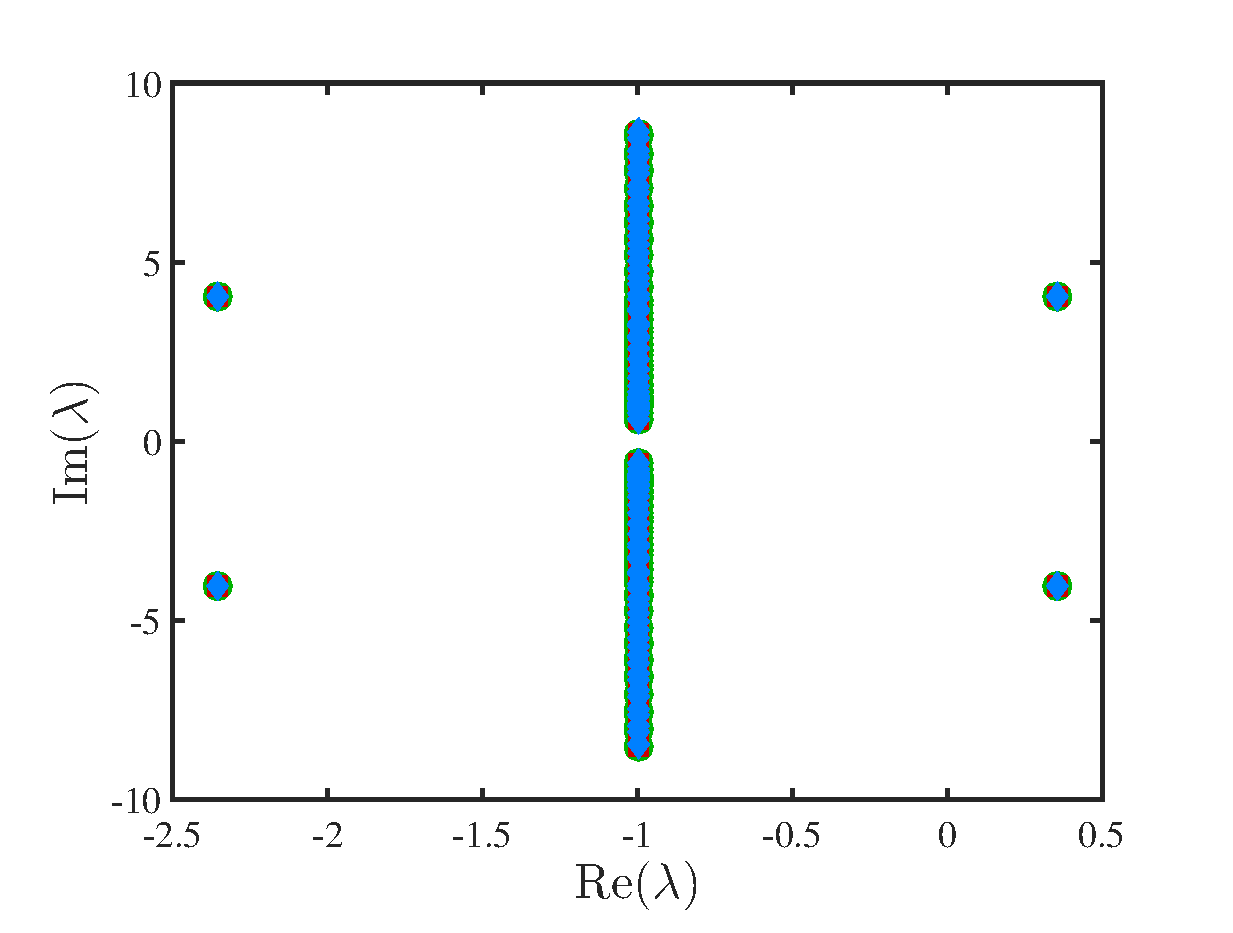
\includegraphics[width=0.9\linewidth]{EigPlot_14.eps}
\caption{$h = 0.5$ }
\end{subfigure}}
  \rule{35em}{0.5pt}
\caption[Comparison of Frequency Spectrum for Domain Length $L=50$]{Comparison of the frequency spectrum for the domain length $L=50$ for (a) $h=0.05$, (b) $h=0.1$, and (c) $h=0.5$.  Each plot has same layout as Fig.~\ref{figAdd1}.  The domain length $L=50$ is adequately contains the steady state solution without truncation; therefore, the solution tends to zero at the boundary.  The three boundary conditions [Dirichlet (green), Neumann (red), and periodic (blue)] converge for $h=0.1$ and $h=0.05$.  The discretization (c) $h=0.5$ is too coarse and does not converge.}
\label{figAdd2}
\end{figure}
}

\JMR{Figure~\ref{figAdd1} compares the frequency spectrum for the three boundary conditions using a domain length $L = 10$ for various discretization [(a) $h = 0.01$, (b) $h= 0.05$, (c) $h=0.1$ and (d) $h = 0.5$ (which truncates the solution)].  In Fig.~\ref{figAdd1}, the Neumann (red) and periodic (blue) boundary conditions are comparable; however the Dirichlet (green) boundary conditions have discrepancies due to imposing an invalid criteria that the solution is zero at the boundary.  %There are discrepancies between a few eigenvalues using the Dirichlet boundary condition due to forcing zero solutions at the boundaries of the domain.  
For domain length $L=10$, the steady state solution is truncated and is not zero along the boundary.  A more accurate choice of Dirichlet boundary condition would be $u(-L/2) = \alpha$ and $u(L/2) = \beta$ where $\alpha$ and $\beta$ are constants.  Figure~\ref{figAdd2} compares the domain length $L=50$ for various discretization [(a) $h = 0.05$, (b) $h=0.1$, and (c) $h=0.5$] for the three boundary conditions.  The larger domain length depicts agreement between all three boundary conditions except for large $h$=0.5 (in agreement with Table~\ref{dxsmall}).  Both Figs.~\ref{figAdd1}(d) and~\ref{figAdd2}(c) show no convergence for $h=0.5$, which is too coarse a step size for use in the LL model.  The numerical discretization, domain length and boundary conditions can influence the stability analysis.  Based on Tables~\ref{dxsmall} and \ref{unstableeigTable}, we can conclude a maximum discretization $h=0.1$ to use for convergence.  As the domain length is increased the convergence also improves but at the cost of a larger matrix size.  For $L\ge 20$ and $h\le 0.1$, the three boundary conditions are in good agreement and converge to the same frequency spectrum.  Based on these results, for the spectrum in Fig.~\ref{fig:frequencySpectrum} we used the Dirichlet boundary condition, domain length $L = 50$ and discretization $h$ = 0.1, which converge to the frequency spectrum for the eigenvalue problem Eq.~(\ref{PDEEigenProblem}).}


%%%%%%%%%% Section Numerical Results
\subsection{Bifurcation Analysis Using the NCVA Approach
\label{secNCVA:app}}
%
We apply the NCVA to Eq.~(\ref{LugiatoLefever}) to verify if the reduced
dynamical system is able to qualitatively (and quantitatively) capture the 
SSB instability by following all temporally symmetric and asymmetric solutions 
to the reduced system of ODEs given by %Eq.~(\ref{NCVAODE}).
%Then, the modified Euler-Lagrange equations for the effective Lagrangian $L = \int_{-\infty}^\infty \mathcal{L}_T d\tau$ yield
%%
\begin{equation}
%\frac{\partial p}{\partial t} = \frac{\partial \mathcal{L}}{\partial u} \equiv \frac{\partial L}{\partial u} + \left[ \frac{\partial R}{\partial u_- }\right]_{\mathrm{PL}}.
\frac{\partial L}{\partial u} - \frac{d}{dt}\left( \frac{\partial L}{\partial \dot{u}} \right) + \int_{-\infty}^\infty \left[ \frac{\partial \mathcal{R}}{\partial u_- }\right]_{\mathrm{PL}} d\tau = 0. 
\label{NCVAODE}
\end{equation}
%
The conservative Lagrangian density for the NLS, namely Eq.~(\ref{LugiatoLefever})
with the right-hand-side equal to zero, is
%
\begin{equation}
\mathcal{L} = \frac{i}{2} \left(u^* u_z- u u_z^*\right) -  \left\vert u_{\tau}\right\vert^2 +  \frac{1}{2}\left\vert u \right\vert^4 - \Delta \left\vert u \right\vert^2.
\end{equation}
%
Here, we construct $\left[ \partial \mathcal{R}/\partial u_- \right]_{\mathrm{PL}} = - iu + i S(\tau)$, by choosing $\mathcal{R} = \left( -iu_{+} + i S(\tau) \right)u_-$.  Therefore, the relevant non-conservative Lagrangian density can be written as
%
\begin{eqnarray}
\mathcal{L} &=& \frac{i}{2} \left(u_{1}^* u_{1,z}- u_{1} u_{1,z}^*\right) -  \left\vert u_{1,\tau}\right\vert^2 + \frac{1}{2} \left\vert u_1 \right\vert^4 -  \Delta  \left\vert u_1 \right\vert^2  \nonumber
 \\
&-& \frac{i}{2} \left(u_{2}^* u_{2,z}- u_{2} u_{2,z}^*\right) +  \left\vert u_{2,\tau}\right\vert^2 -\frac{1}{2}  \left\vert u_2 \right\vert^4 +  \Delta  \left\vert u_2 \right\vert^2  \nonumber \\ 
&+& \left( - iu_{+} + i S(\tau) \right)u_-,  
\end{eqnarray}
%
where $u_1 = \left( 2u_+ + u_- \right)/2$ and $u_2 = \left(2u_+ - u_- \right)/2$.
%
For reasons of brevity, we chose to express the Lagrangian density above
in 1,2 coordinates. Writing the Lagrangian in $\pm$ coordinates lends
itself to lengthier expressions but to more straightforward implementation
of the physical limit where the (+) variables directly coincide with the
physical variables [and the $(-)$ variables are eliminated].
%
From $\mathcal{L} $, we can derive, through the Euler-Lagrange
equations (\ref{NCVAODE}), the full LL model at the PDE level.
In order to, however, obtain an analytical insight in the dynamics
of the model, our aim is to use an ansatz approximation of the
pulse reducing its Lagrangian to a Lagrangian over effective
(yet time-dependent) properties of its form, like the amplitude,
the width and its center of mass, among others. Then for these
effective properties, in the spirit of Refs.~\cite{JuliaNCVA,ref4},
a coupled system of 
ODEs approximating
the dynamical evolution will be derived and, perhaps more
importantly for our considerations, their corresponding steady
states and possible bifurcations will be amenable to 
analysis. 

Applying the NCVA methodology described above to the LL model
(\ref{LugiatoLefever}) where \begin{align}
\left[ \frac{\partial \mathcal{R}}{\partial
u_- }\right]_{\mathrm{PL}} = -iu  + i S(\tau), \end{align}
 yields 
\begin{align}
\mathcal{R} = \left( -iu_{+}  + i S(\tau) \right)u_-.
\end{align}  
%
We first choose the following simple Gaussian ansatz
%
\begin{equation}
\bar{u}_j = a_j \exp\left[-\frac{(\tau-\xi_j)^2}{2\sigma_j^2}\right] \exp(i\,b_j),
\quad j=1,2
\label{eq:4pAnsatz}
\end{equation}
%
where height $a$, center position $\xi$, width $\sigma$, and phase $b$ 
are the variational parameters.  
%
The ansatz was selected as the simplest localized waveform with freedom
to move left or right in order to capture, in the simplest sense,
a possible asymmetry in the solution of the original LL model.
%
Applying the NCVA method with this, arguably 
over-simplified, four-parameter ansatz, 
leads, through the Euler-Lagrange equations, to a system of algebraic 
differential equations for which the derivatives of the variational
parameters cannot be solved for explicitly. Nonetheless, it is
possible to obtain algebraic equations for the corresponding 
steady state ($\dot{a} = \dot{b} = \dot{\xi} = \dot{\sigma} = 0$)
solutions of the form:
%
\begin{align}
%\setlength{\jot}{16pt}
%\begin{cases}
%\frac{a^2\sqrt{\pi}}{2 \sigma^2}+\frac{1}{4} a^4\sqrt{2 \pi}+\Delta a^2\sqrt{\pi} &= \frac{2a\sqrt{X}\sin(b)\sqrt{2\pi}T_0^3}
%{(T_0^2+2\sigma^2)^{3/2}}, \\[1em] \nonumber
%2a^2\sigma\sqrt{\pi} &= \frac{2 \sqrt{X}a\cos(b)\sqrt{2\pi}\sigma T_0}{\sqrt{T_0^2+2\sigma^2}}, \\[1em] \nonumber
%-\frac{a\sqrt{\pi}}{\sigma}+a^3\sqrt{2\pi}\sigma+2\Delta a\sigma\sqrt{\pi} &= \frac{2\sqrt{X}\sin(b)\sqrt{2\pi}\sigma T_0}
%{\sqrt{T_0^2+2\sigma^2}}, \\[1em] \nonumber
%0 &= \frac{-2\sqrt{X}a\xi\sin(b)\sqrt{2\pi}T_0}{\sigma\sqrt{T_0^2+2\sigma^2}}. \\
%\end{cases}
%\end{align}
\begin{cases}
\frac{a^2\sqrt{\pi}}{2 \sigma^2}+\frac{1}{4} a^4\sqrt{2 \pi}+\Delta a^2\sqrt{\pi} &= \frac{a\sin(b)T_0^2 \beta}
{(T_0^2+2\sigma^2)}, \\[1em]
2a^2\sigma\sqrt{\pi} &=  a \cos(b) \sigma \beta, \\[1em]
-\frac{a\sqrt{\pi}}{\sigma}+a^3\sqrt{2\pi}\sigma+2\Delta a\sigma\sqrt{\pi} &= \sin(b) \sigma \beta, \\[1em]
0 &= \frac{-a\xi\sin(b)\beta}{\sigma},
\end{cases}
\label{4pE}
\end{align}
%
where $\beta = \frac{2\sqrt{2 \pi X} T_0}{\sqrt{T_0^2 + 2 \sigma^2}}$.  


Figure~\ref{figSSB4p} depicts the comparison of the bifurcation diagrams
for steady state solutions obtained from the original LL 
model~(\ref{LugiatoLefever}) and the NCVA approach for $\Delta =0.92$ 
and $T_0=2.3$ by monitoring $|u (\tau=0)|^2$ as a function of pump 
peak power $X$, in line with the earlier work of Ref.~\cite{XuCoen}.
%
Both solutions for the original LL model and the algebraic NCVA system
are obtained by numerical continuation using a standard fixed point iteration 
(Newton-Krylov).
%
The solutions for the LL model are depicted by the thick curves
while the corresponding NCVA approximations by the thin curves.
Solid and dashed correspond, respectively, to stable and unstable 
solutions.
%
The insets in the figure depict temporal pulse intensity profiles 
$|u|^2$ for $X = 4$ (symmetric), $X=8$ (symmetric and asymmetric), 
and $X=11$ (symmetric) for both the LL model (thick curves)
and the NCVA reconstructions (thin curves).
%
For completeness, the insets also show the corresponding linearization
spectra.
%
As it is evident from the figure, the NCVA with a four-parameter 
ansatz agrees very well with the symmetric branch of LL model
(see black and blue curves). However, for the asymmetric branch
there seems to be a large discrepancy between the LL model and
its NCVA approximation. In fact, as indicated in the figure, the 
asymmetric NCVA branch is unstable while it is stable for the original 
LL model. Upon further inspection (details are omitted for brevity), 
the instability of the asymmetric NCVA branch stems, instead of
a pitchfork bifurcation, from a Hopf bifurcation that creates a stable 
limit cycle in the variational parameters.
%
%%%%%%%%%% Fig 3 %%%%%%%%%%%%%%%%%%%%%%%%%%%%%%%%%%%%%%
\begin{figure*}[t!!]
\centering
\centerline{
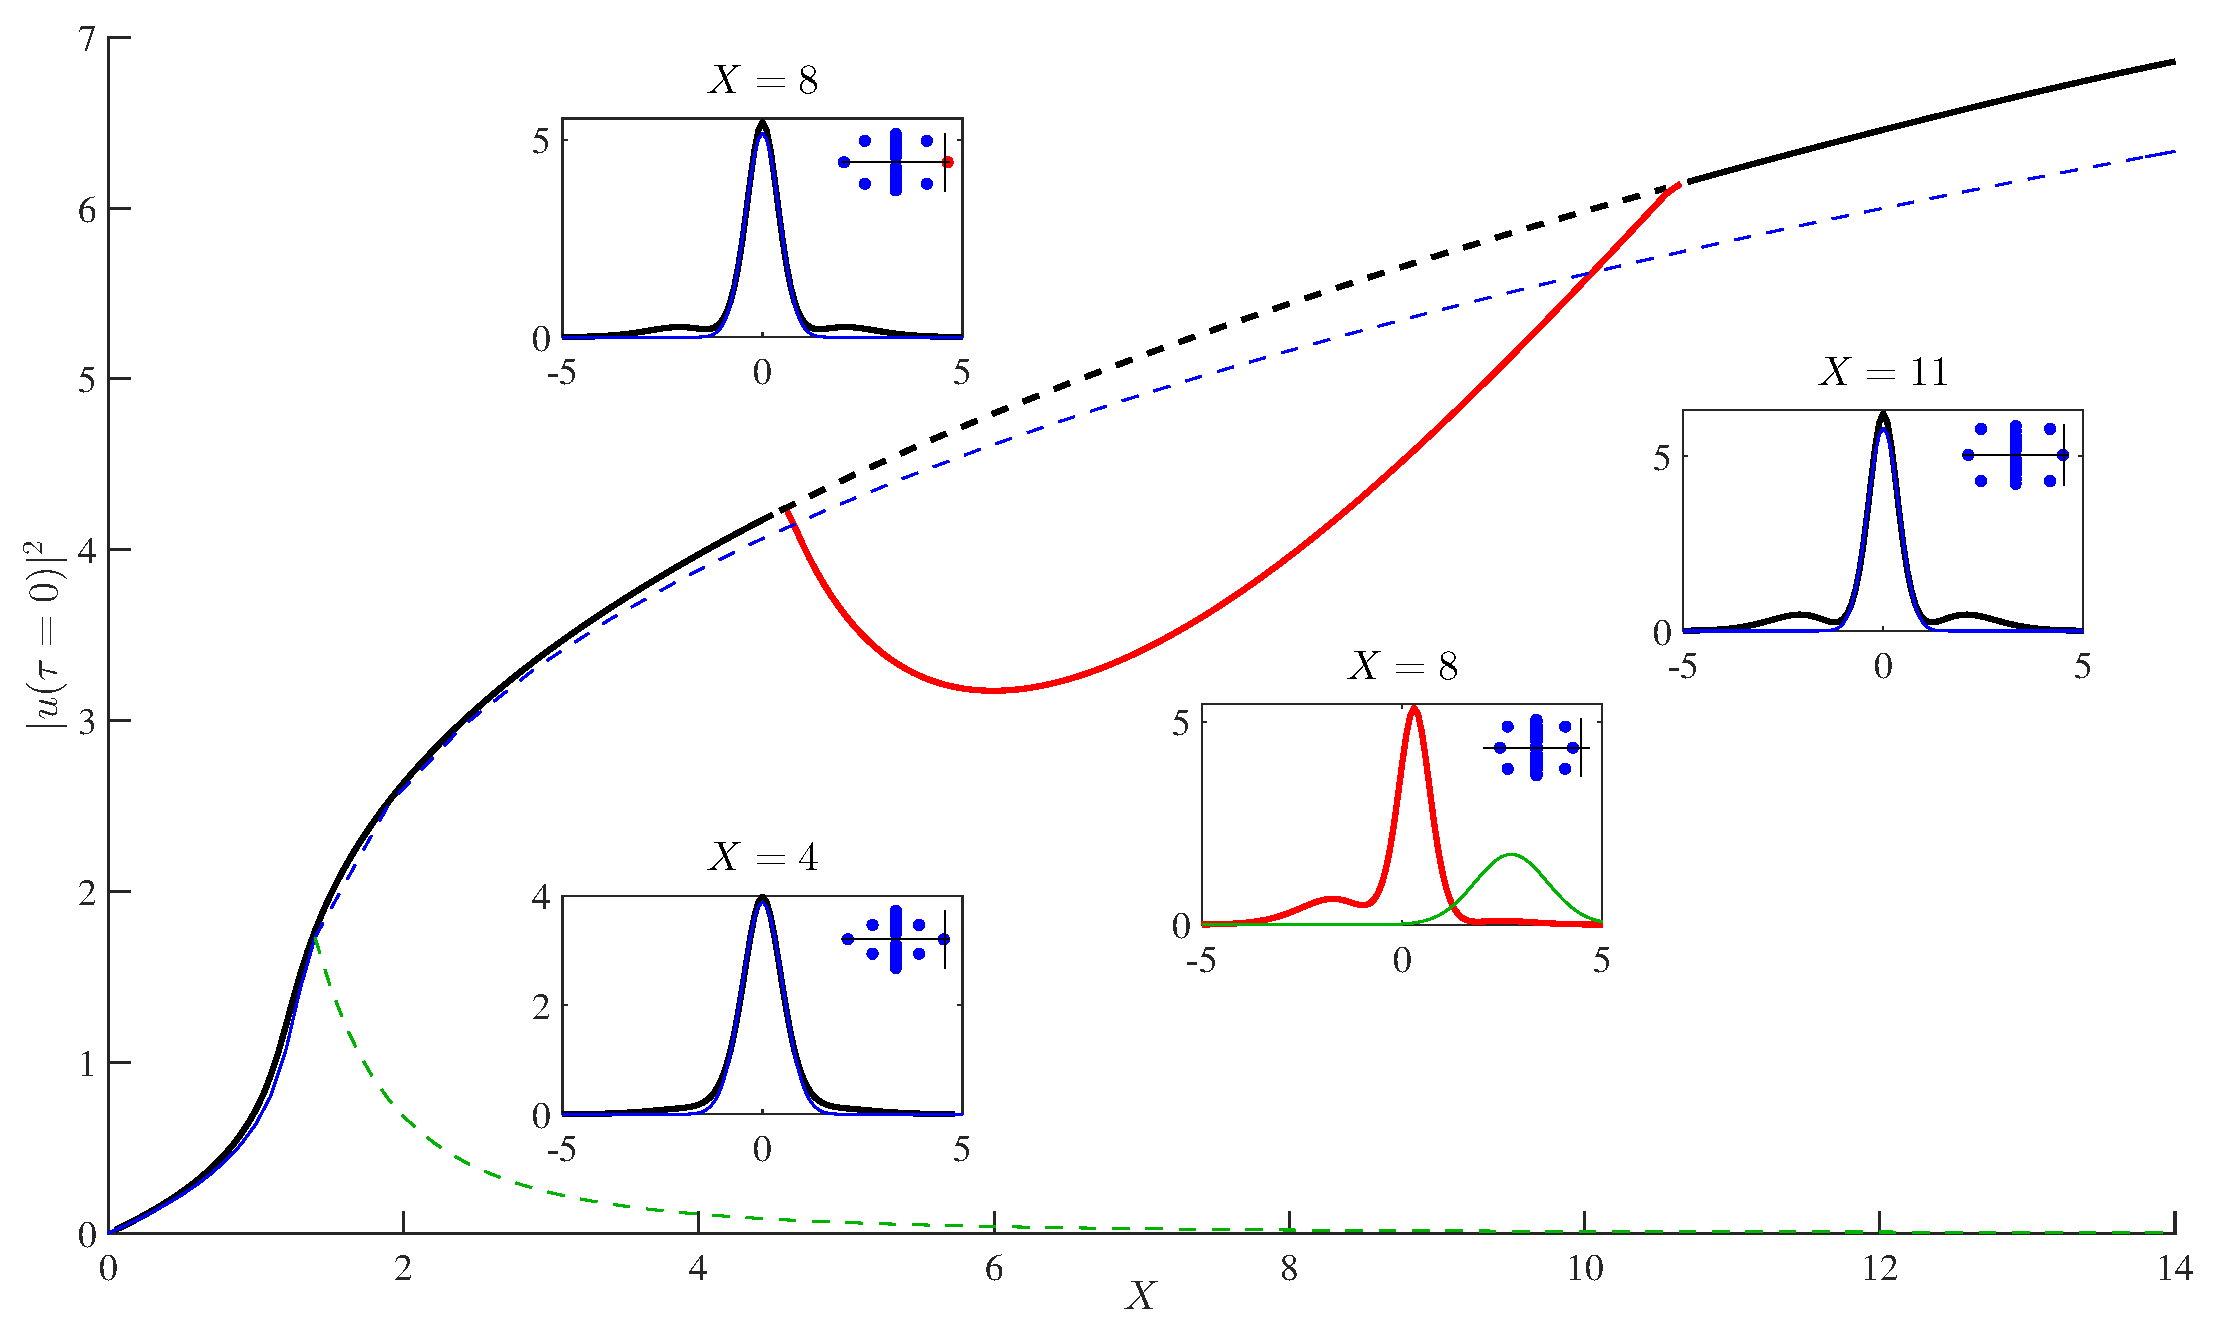
\includegraphics[width=0.95\textwidth]{SSBBif4PN.eps}}
  \rule{35em}{0.5pt}
\caption[SSB Bifurcation Diagram Comparison for LL Steady States and NCVA 4-Parameter Ansatz]{Bifurcation for steady states of the LL model (\ref{LugiatoLefever})
(thick curves) and their approximation using the NCVA methodology with the 
over-simplified four-parameter ansatz (\ref{eq:4pAnsatz}) (thin curves)
as the pump strength $X$ is varied for $\Delta = 0.92$ and $T_0 = 2.3$.
%
Stable (Unstable) branches are depicted with solid (dashed) lines.
%
The (red and green) branches bifurcating from the main branch (blue and 
black lines) correspond to asymmetric solutions.
%
The insets depict the pulse temporal intensity profiles obtained for 
$X=4, 8$ (symmetric and asymmetric), and $X=11$ (symmetric) for
the original LL model (thick curves) and their NCVA approximation
(thin curves).
%
The insets also depict the corresponding stability spectra
for these solutions where stable eigenvalues are depicted in blue 
and unstable eigenvalues in red.
\label{figSSB4p}}
\end{figure*}
%%%%%%%%%% Fig 3 %%%%%%%%%%%%%%%%%%%%%%%%%%%%%%%%%%%%%%

It is evident that the four-parameter ansatz is unable to predict the
existence of the pitchfork loop of the original LL model and, furthermore,
although it is able to predict a SSB bifurcation, it fails to give an 
accurate estimation for its threshold (i.e., the critical
pump power needed to observe asymmetric states).
%
However, this over-simplified ansatz gives two valuable insights regarding 
how to make a more judicious choice for our ansatz. 
%
Firstly, the ansatz~(\ref{eq:4pAnsatz}) has an inherent complication in that
its corresponding Euler-Lagrange equations lead to a degenerate system
of differential-algebraic equations which can only be explicitly written
for the steady state. 
%
This degeneracy can be circumvented, as we will show below, by proper balancing 
of the variational parameters in an ansatz with more degrees of freedom.
%
Secondly, and more importantly, the four-parameter ansatz, by construction, 
only corresponds to real solutions (up to a global phase shift) that lack a 
$\tau$-dependence on their phase.
%
This lack of $\tau$-dependence on the phase is responsible for the
ansatz solution's lack of internal flow of the field $u$
along the $\tau$-direction.  To showcase the importance of a nontrivial $\tau$-dependence on the phase, on may transform the NLS equation through the Madelung transformation $u=\sqrt{\rho}\,e^{i\phi}$ such that the wavefunction is recast in terms of its density $\rho$ and phase $\phi$.  Through the Madelung transform, we can obtain an evolution equation for the density that corresponds to an inviscid Eulerian fluid with the fluid velocity $v$ given precisely by $v = \nabla \phi$.  Thus, the fluid velocity for the system can be obtained by computing
the gradient of the phase of the solution at hand.
Therefore, a lack of a phase variation in the solution
implies a lack of internal fluid flow for the solution. 
%
%\footnote{We remind the reader that when transforming the
%NLS equation through the Madelung transformation
%$u=\sqrt{\rho}\,e^{i\phi}$ (i.e., writing the wavefunction in
%terms of its density $\rho$ and phase $\phi$), one obtains
%an evolution equation for the density that corresponds to
%an inviscid Eulerian fluid (incorporating the so-called
%quantum pressure term that is not important for the current
%argument) with the fluid velocity $v$ given precisely by $v=\nabla \phi$.
%Thus, the fluid velocity for the system can be obtained by computing
%the gradient of the phase of the solution at hand.
%Therefore, a lack of a phase variation in the solution
%implies a lack of internal fluid flow of the solutions.}
%
As we explain below, the asymmetric solution is supported
by a delicate balance of the internal flow within this
steady state solution. 
%albeit the density
%of the solution remaining constant (i.e., it is a steady state
%for the density).
%
The presence of the underlying flow is clear after careful examination
of the (numerically) exact solutions of the original LL model as depicted
in panels (a) and (b) of Fig.~\ref{fig4SSB}. These panels depict the
density (blue) and phase (red) of the solution where the arrows
indicate the regions where the fluid velocity, as defined by the
gradient of the phase, has different directions. 
%
The central density maximum, for both the symmetric and
asymmetric solutions, stems from an inward flow towards the
center [which corresponds to a sink of flow due to high density 
through the loss term $iu$ in Eq.~(\ref{LugiatoLefever})]
while the ``wings'', again for both symmetric and asymmetric solutions, 
are supported by sources of the underlying flow maintained by
the pump.
%
In contrast, the NCVA four-parameter ansatz (\ref{eq:4pAnsatz}) lacks
a phase profile and, therefore, lacks any internal flow as depicted
in panels (c) and (d) of Fig.~\ref{fig4SSB}.
%
It is then clear that the four-parameter ansatz (\ref{eq:4pAnsatz})
should be inadequate for capturing the important effects of
the underlying current flows of the solutions.

%%%%%%%%%% Fig 4 %%%%%%%%%%%%%%%%%%%%%%%%%%%%%%%%%%%%%%%%%%%%%%%%%%%%%%
\begin{figure}[t!]
\centering
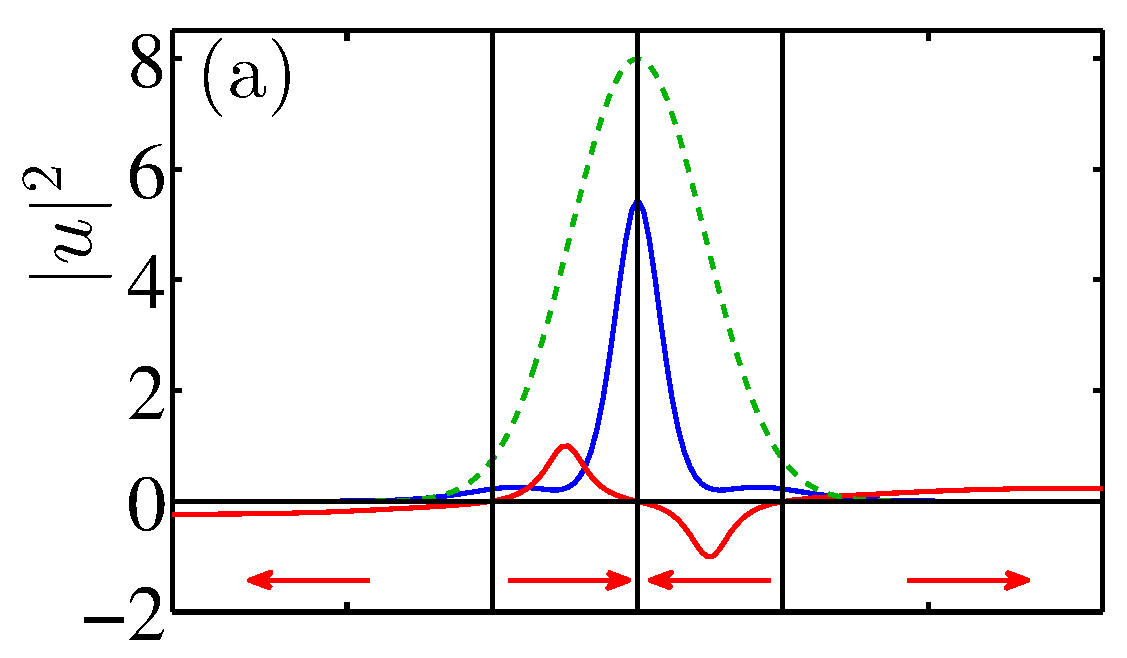
\includegraphics[width=0.42\textwidth]{fluidVelocity_X8_pdeSN.eps} \quad
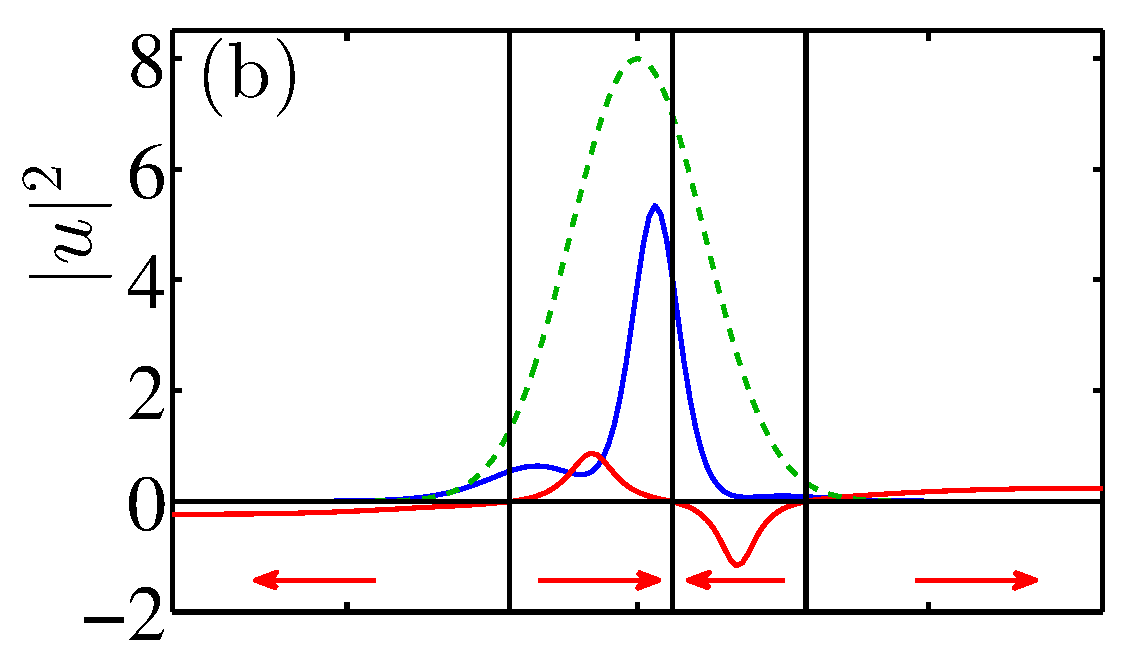
\includegraphics[width=0.42\textwidth]{fluidVelocity_X8_pdeASN.eps}
\\
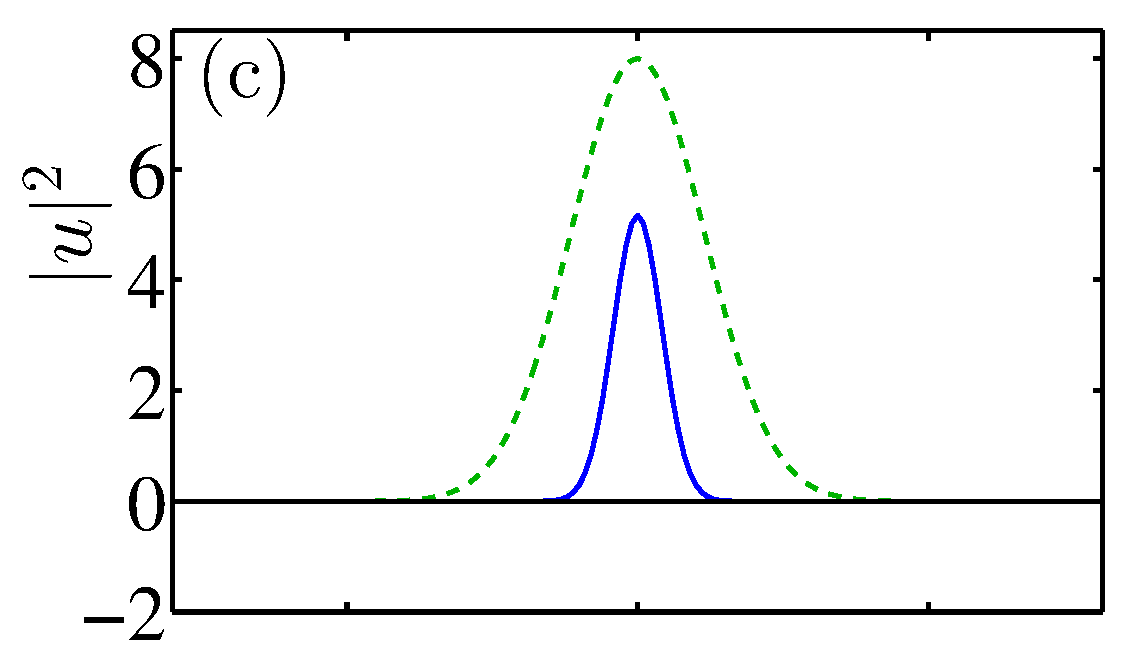
\includegraphics[width=0.42\textwidth]{fluidVelocity_X8_4PSN.eps} \quad
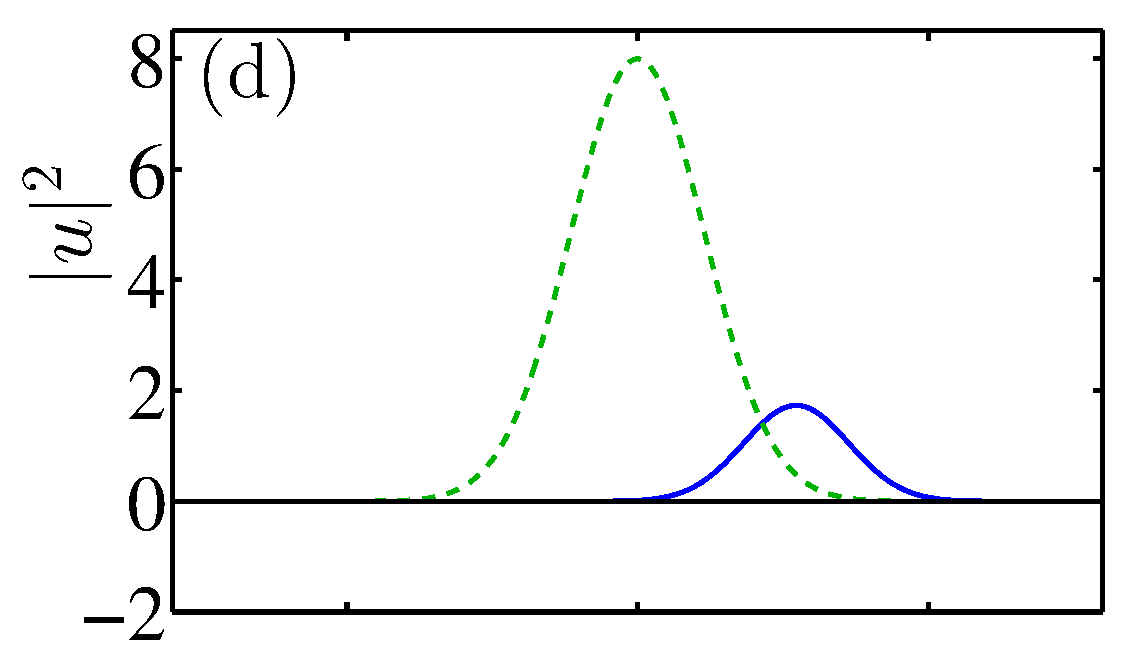
\includegraphics[width=0.42\textwidth]{fluidVelocity_X8_4PASN.eps}
\\
\centerline{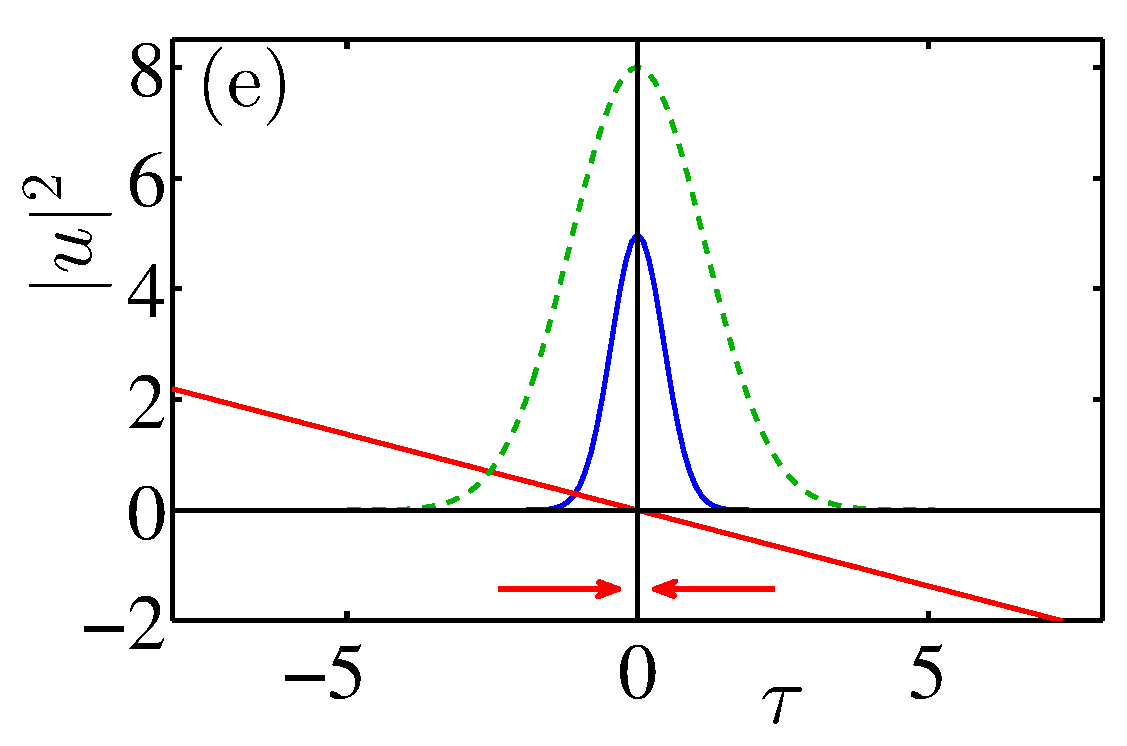
\includegraphics[width=0.42\textwidth]{fluidVelocity_X8_6PSN.eps} \quad
\includegraphics[width=0.42\textwidth]{fluidVelocity_X8_6PASN.eps}}
%\vskip -1.5cm
  \rule{35em}{0.5pt}
\caption[Fluid Velocity of LL Equation and NCVA Solutions]{Understanding the importance of including non-trivial phase
terms in the NCVA ansatz. The different panels depict an overlay of 
(i) the temporal intensity profile of the pump pulse $|S(\tau)|^2$ 
(green dashed line),
(ii) the pulse intensity profile $|u|^2$ (blue), and 
(iii) its corresponding fluid velocity (red, $\times 50$)
for 
(a,b) the LL model (top), 
(c,d) the four-parameter NCVA (middle), and 
(e,f) the six-parameter NCVA (bottom)
for symmetric $X=8$ (left) and asymmetric $X=8$ (right) steady state solutions.
%
The (red) arrows indicate the direction of the fluid velocity which drives 
the SSB bifurcation between the symmetric and asymmetric solutions.
}
\label{fig4SSB}
\vskip -0.5cm
\end{figure}
%%%%%%%%%% Fig 4 %%%%%%%%%%%%%%%%%%%%%%%%%%%%%%%%%%%%%%%%%%%%%%%%%%%%%%


It is important to mention at this stage that steady state solutions
(for the density) in NLS-type settings incorporating loss and gain
terms must necessarily involve underlying flows that carry
``material'' from the gain regions towards the lossy regions.
%
Therefore, in these settings, variational methods should be based
on ans\"atze that incorporate the appropriate underlying current.
%
Inspired by the appreciation of the presence of such underlying flows 
(and their delicate balance in the steady state solutions)
let us choose an ansatz that is capable of supporting such flows.
%
Based on this observation, we introduce a six-parameters ansatz
of the form:
%
\begin{eqnarray}
\bar{u}_j &=&  a_j \exp\left[\frac{-(\tau-\xi_j)^2}{2\sigma_j^2}\right] \;  \exp\left[i(d_j(\tau-\xi_j)^2 + c_j(\tau - \xi_j) + b_j)\right] ,
\label{6pansatz}
\end{eqnarray}
%
where, in addition to the parameters height $a$, center position $\xi$, 
width $\sigma$, phase $b$, we have also introduced  velocity $c$ and 
chirp $d$ as variational parameters.
%
Following again the NCVA methodology for this improved ansatz, we 
obtain the following system of ODEs of the variational parameters:
%
\begin{align}
\begin{cases}
\dot{a} =& \frac{1}{4}\frac{-4a^2\sigma^3\sqrt{\pi}+3\sigma^2I_b-8a^2d\sigma^3\sqrt{\pi}-2I_d}{a\sigma^3\sqrt{\pi}}, \\[1em]
\dot{b} =& -\frac{1}{8}\frac{8a^2\sqrt{\pi}-5a^4\sqrt{2}\sqrt{\pi}\sigma^2-4I_\sigma \sigma^2+6I_a\sigma a-8a^2c^2\sqrt{\pi}\sigma^2}{ a^2\sigma^2\sqrt{\pi}} + \frac{\sigma c I_c-a^2 \Delta\sqrt{\pi}\sigma^2}{a^2\sigma^2\sqrt{\pi}}, \\[1em]
\dot{c} =& -\frac{c I_b+I_{\xi}}{a^2\sigma\sqrt{\pi}}, \\[1em]
\dot{d} =& \frac{1}{4}\frac{4a^2\sqrt{\pi}-16a^2 d^2 \sigma^4\sqrt{\pi}-a^4\sqrt{2}\sqrt{\pi}\sigma^2-4I_s\sigma^2+2I_a\sigma a}
{a^2\sigma^4\sqrt{\pi}}, \\[1em]
\dot{\sigma} =& -\frac{1}{2}\frac{\sigma^2I_b-8a^2 d \sigma^3\sqrt{\pi}-2I_d}{a^2\sigma^2\sqrt{\pi}}, \\[1em]
\dot{\xi} =& \frac{2a^2\sigma c \sqrt{\pi}+I_c}{a^2\sigma\sqrt{\pi}}, 
\end{cases}
\label{6pE}
\end{align}
%
where the over-dot denotes derivative with respect to $z$.  Although it is possible to explicitly solve for the derivatives
of the variational parameters, the resulting NCVA ODEs are cumbersome
in that they include the terms $I_a, I_b, I_c, I_d, I_{\xi},$ and 
$I_{\sigma}$ which involve integrals that cannot be explicitly evaluated:
%
\begin{align}
\begin{cases}
I_a =& \bigintss\limits_{-\infty}^{\infty} E\sin(\Phi) \,d\tau, \\[0em] \nonumber
I_b =& \bigintss\limits_{-\infty}^{\infty} aE \cos(\Phi) \,d\tau, \\[0em]
\nonumber
I_c =& \bigintss\limits_{-\infty}^{\infty}  a E(\tau-\xi) \cos(\Phi) \,d\tau, \\[1em]
\nonumber
I_d  = &\bigintss\limits_{-\infty}^{\infty} a E(\tau-\xi)^2 \cos(\Phi) \,d\tau ,\\[1em] \nonumber
I_\sigma =&\bigintss\limits_{-\infty}^{\infty} \frac{ a E}{\sigma^3}  \sin(\Phi) \,d\tau,  \\[1em] \nonumber
I_\xi =&\bigintss\limits_{-\infty}^{\infty} \Big[aE \left(-2d(\tau-\xi)-c\right)
\cos(\Phi)  + \frac{ a E(\tau-\xi) }{\sigma^2} \sin(\Phi) \Big] \,d\tau, 
\end{cases}
\end{align}
%
where $\Phi =d(\tau-\xi)^2+c(\tau-\xi)+b$ and $E = 2\sqrt{X}e^{-\frac{ (\tau-\xi)^2}{2 \sigma^2}}e^{-\frac{\tau^2}{T_0^2}} $.
%
Nonetheless, for our numerical studies it suffices to evaluate numerically
these integrals as we seek stationary states or as we follow the
dynamics of the parameters as $z$ changes.

%%%%%%%%%% Fig 5 %%%%%%%%%%%%%%%%%%%%%%%%%%%%%%%%%
\begin{figure}[htb!]
\centering
\centerline{
\includegraphics[width=0.9\textwidth]{frequencySpectrum_NCVA.eps}}
  \rule{35em}{0.5pt}
\caption[NCVA ODE Linearization Spectrum]{
Linearization spectrum for the reduced NCVA ODE (\ref{6pE}).
The notation is the same as the spectrum for the original LL model
depicted in Fig.~\ref{fig:frequencySpectrum}.
%
The reduced ODE model displays a degenerate bifurcation
consisting of simultaneous pitchfork (P) and Hopf (H)
bifurcations and thus the asymmetric steady state (see thin black
solid lines) is unstable from its inception.
\label{fig:frequencySpectrum_NCVA}
}
\end{figure}
%%%%%%%%%% Fig 5 %%%%%%%%%%%%%%%%%%%%%%%%%%%%%%%%%

%%%%%%%%%% Fig 6 %%%%%%%%%%%%%%%%%%%%%%%%%%%%%%%%%%%%%%%
\begin{figure*}[htb!]
%\vspace{-0.5cm}
\centering
\centerline{
\includegraphics[width=0.95\textwidth]{SSBBif6PN.eps}}
\caption[SSB Bifurcation Diagram Comparison for LL Steady States and NCVA 6-Parameter Ansatz]{Bifurcation diagram as in Fig.~\ref{figSSB4p} but for the more 
complete six-parameter ansatz (\ref{6pansatz}). Same layout and
meaning as in Fig.~\ref{figSSB4p}.}
\label{figSSB6p}
\end{figure*}
%%%%%%%%%% Fig 6 %%%%%%%%%%%%%%%%%%%%%%%%%%%%%%%%%%%%%%%

Figure \ref{fig:frequencySpectrum_NCVA} depicts the linearization
spectrum for the reduced NCVA six-parameter ODE model (\ref{6pE}) that 
should be compared to the linearization spectrum of original LL model
depicted in Fig.~\ref{fig:frequencySpectrum}.
%
It is clear that both spectra share some of the bifurcation structure 
but, at the same time, they have notable differences.
%
For instance, although the reduced NCVA ODE is able to capture
the SSB at $X\approx 3.8$, reasonably close to the actual bifurcation 
of the original model at $X\approx 4.6$, the bifurcation, instead of
being a pitchfork one, is a degenerate one comprising simultaneous 
pitchfork and Hopf bifurcations.
%
This is the reason why the reduced ODE NCVA model transitions directly
from a stable symmetric solution to a stable (asymmetric) periodic 
limit cycle instead of a stable asymmetric steady state as in 
the original LL model.
%
The bifurcation diagram for the six-parameter ansatz (\ref{6pansatz}),
together with the one from the original LL model, is depicted in 
Fig.~\ref{figSSB6p} using the same layout as Fig.~\ref{figSSB4p}.  
%
As it is clear for comparing Figs.~\ref{figSSB4p} and \ref{figSSB6p},
the six-parameter ansatz does a much better job at capturing the
asymmetry states (see insets) and the threshold for the primary
SSB bifurcation than its four-parameter counterpart.
%
However, as we noted above (and similar to the case of the reduced 
four-parameter NCVA ode) the bifurcation predicted by
the NCVA ODEs (\ref{6pE}) produces an unstable asymmetric state
and a stable (asymmetric) periodic limit cycle.
%
Nonetheless, the six-parameter is now able to capture the essence 
of the underlying flow as it can be seen from panels (e) and (f)
of Fig.~\ref{fig4SSB}.
%
Furthermore, and perhaps more importantly, the improved six-parameter 
NCVA approach is also able to predict reasonably well the threshold 
for the pump power for the onset of the SSB bifurcation.
%
The fact that the NCVA method is insufficient in characterizing the
details of the SSB instability is, arguably, 
the consequence of employing ans\"atze 
that (while remaining tractable) 
lack the proper freedom to include underlying flows that are
akin to the solutions displayed by the original LL model.
%
For instance, in order to capture the details of the underlying flows
depicted in panels (a) and (b) of Fig.~\ref{fig4SSB} it should be
necessary to include a fluid flow that has, at least, three
zeros and that would entail, if using polynomials as a basis
for expanding the phase, a quartic polynomial (i.e., five
parameters) for the phase.
%
Such an ansatz would require five phase variational parameters
and five shape (density) parameters leading to a cumbersome system
of ten couple ODEs. Such a venture falls outside of the scope
of the present dissertation.
%

%%%%%%%%%%%%% Section: Pitchfork Bifurcation based on Mariana notes
\subsection{Local Bifurcation Analysis
\label{secGalerkin}}

In this section, we employ a \JMR{center manifold reduction to determine} 
the dynamics of the system close to the pitchfork bifurcations (theory below developed in part by Mariana Haragus). 
\JMR{
Center manifold reductions are extensively used in the analysis of local bifurcations. Starting from a dynamical system formulation of the bifurcation problem, the reduction to a center manifold provides the lowest dimensional dynamical system which fully describes the original dynamics close to a bifurcation point. We use this method to analyze the two pitchfork bifurcations which arise in  Eq.~(\ref{NLSEq}) as $X$ is increased. As a result we obtain, in both cases, a reduced scalar ordinary differential equation which captures the bifurcating dynamics. The first two coefficients in the expansion of the reduced scalar field, which are computed numerically here, determine the type of the bifurcation. They are also essential in the computation of the bifurcating asymmetric states and of the local temporal dynamics. 
} 

Let us consider Eq.~(\ref{NLSEq}) with, as before, $\eta=-1$.
%
In order to reduce the bifurcation analysis to real variables we rewrite
\begin{align}
E = U + iV,
\label{realvar}
\end{align}
where $U$ and $V$ are real fields. Then, the model~(\ref{NLSEq})
is equivalent to the system
\begin{align}
%\begin{cases}
U_z = -U -V_{\tau\tau} + \Delta V - (U^2 + V^2)V + S(\tau),\\
% \sqrt{X} e^{-(\tau/T_0)^2},\\
V_z = -V + U_{\tau\tau} - \Delta U + (U^2 + V^2) U.
%\end{cases}
\end{align}
%
By using the implicit function theorem we can show that, for any $X$ sufficiently small, there exists a unique steady state solution $(U_X(\tau), V_X(\tau))$, which is even in $\tau$ and exponentially decaying to 0 as $|\tau| \rightarrow \infty$.  The previous numerical computations in Fig.~\ref{figSSB6p} show the steady state solutions for values of $X$ between 0 and 14 and can be continued for larger values of $X$.  For this analysis we are only interested in possible bifurcations, and in particular, in the two pitchfork bifurcations predicted by numerical computations at $X_1$ = 4.596695 and $X_2$ = 10.604008, respectively.

For our analysis, we define a new dynamical system with solutions close to 
the bifurcation $(U_X, V_X)$, and therefore set
\begin{eqnarray}
\label{pertu}
U = U_X + \nu, \quad \quad V = V_X + v,
\end{eqnarray}
%
where $\nu$ and $v$ describe the deviations from the steady state. We thus 
obtain the new system:
%
%\begin{align*}
%\nu_z =& -\nu -(v_{\tau \tau} - \Delta v + 2 U_X V_X \nu + (U_X^2 + 3V_X^2) v \\
%&+ V_X \nu^2 + 2 U_X \nu v + 3V_X v^2 + (\nu^2 + v^2)v),\\
%v_z =& -v +(\nu_{\tau \tau} - \Delta \nu + (3U_X^2+V_X^2)\nu + 2U_X V_X v \\
%&+ 3U_X \nu^2 + 2V_X \nu v + U_X v^2 + (\nu^2 + v^2)\nu).
%\end{align*}
%The resulting system may be written in the form
\begin{align}
w_z = \mathcal{A}_Xw + \mathcal{J}(\mathcal{R}_{2} (w, w) + \mathcal{R}_3 (w)),
\label{bif1}
\end{align}
%
for the perturbation $w = (\nu, v)^T$, 
where $\mathcal{A}_X$ is the matrix linear operator 
%
\begin{align}
\mathcal{A}_X = -\mathbb{I} + \mathcal{J}\mathcal{L}_X,  
\label{Ax}
\end{align}
%
$\mathbb{I} $ is the identity matrix,
%
\begin{align}
\mathcal{J} = \begin{pmatrix} 0 & -1 \\ 1 & 0  \end{pmatrix}.
\nonumber
\end{align}
%
$\mathcal{L}_X$ is the linear operator defined by
%
\begin{align}
\mathcal{L}_X = \begin{pmatrix} \partial^2_{\tau} - \Delta + 3 U_X^2 + V_X^2 & 2U_X V_X \\ 2 U_X V_X & \partial^2_{\tau} - \Delta + U_X^2 + 3V_X^2 \end{pmatrix},
\nonumber
\end{align}
%
and $\mathcal{R}_{2} (w_1, w_2)$  is the bilinear map given by
%
\begin{align}
\mathcal{R}_{2} (w_1,w_2) = \begin{pmatrix} 3U_X \nu_1 \nu_2 + V_X (\nu_1 v_2 + \nu_2 v_1) + U_X v_1 v_2 \\
V_X \nu_1 \nu_2 + U_X (\nu_1 v_2 + \nu_2 v_1) + 3 V_X v_1 v_2 \end{pmatrix},
\nonumber
\end{align}
%
with $w_1 =  (\nu_1, v_1)^T$ and $w_2 = (\nu_2, v_2)^T$.  
%
Finally, the cubic map $\mathcal{R}_{3} (w)$ is given by
%
\begin{align}
\mathcal{R}_3 (w) = \begin{pmatrix} (\nu^2 + v^2)\nu \\ (\nu^2 + v^2)v  \end{pmatrix},
\nonumber
\end{align}
%
with $w = (\nu, v)^T$.  
%
We choose for Eq.~(\ref{bif1}) the phase space $H = L^2(\mathbb{R}) \times L^2(\mathbb{R})$ equipped with the usual scalar product
%
\begin{align}
\langle w_1, w_2 \rangle = \int_\Omega (\nu_1(\tau)\nu_2(\tau) + v_1(\tau)v_2(\tau)) d\tau,
\nonumber
\end{align}
%
where $\Omega=(-\infty,+\infty)$ is the entire domain.
%
In this Hilbert space $\mathcal{A}_X$ is a closed operator with domain $H^2(\mathbb{R}) \times H^2 (\mathbb{R})$, and the operators $\mathcal{J}$ and $\mathcal{L}_X$ are skew- and self-adjoint, respectively.  The nonlinear terms $\mathcal{R}_{2}$ and $\mathcal{R}_3$ are smooth maps.
%

The bifurcation points are determined by the spectrum of the linear operator $\mathcal{A}_X$, and in particular by the imaginary points in its spectrum.  Since $\mathcal{A}_X$ is a differential operator with asymptotically constant coefficients, its essential spectrum coincides with the spectrum of the asymptotic operator $\mathcal{A}_0$.  A standard Fourier analysis then shows that the essential spectrum is the set
%
\begin{align}
\nonumber
\sigma_{\rm ess} = \{ -1 \pm i (k^2 + \Delta),  \; k \in \mathbb{R} \},
\end{align}
%
which lies in the open left half complex plane.
%

The point spectrum of $\mathcal{A}_X$ consists of eigenvalues with finite algebraic multiplicities.  Notice that due to the structure of $\mathcal{A}_X$, Eq.~(\ref{Ax}), its spectrum is symmetric with respect to the vertical shift 
Re$(\lambda) = -1$ in the complex plane.  It is also symmetric with respect to the real axis, since the operator is real.
%
These two properties are clearly satisfied by the numerically obtained
linearization spectrum depicted in Fig.~\ref{fig:frequencySpectrum}.
%
For sufficiently small $X$, standard perturbation arguments show that the spectrum of $\mathcal{A}_X$ stays close to the one of $\mathcal{A}_0$.  In particular, it lies in the left half complex plane, and no bifurcations occur for small $X$.  Numerical computations show that there exists a first value $X_1$ at which one (simple) eigenvalue crosses the origin and becomes positive for $X > X_1$
(see point $P_1$ in Fig.~\ref{fig:frequencySpectrum}).  
%
All other eigenvalues have negative real parts.  Increasing $X$, there is a second value $X_2$ where this simple eigenvalue crosses the origin back in the left half complex plane
(see point $P_2$ in Fig.~\ref{fig:frequencySpectrum}).
%
Our purpose is to the study the two (pitchfork) bifurcations which occur at 
these parameter values, and which are directly related
to the SSB phenomena observed experimentally in Ref.~\cite{XuCoen}.

We denote by $\lambda_0(X)$ the simple eigenvalue above, so that we have
\begin{align*}
\sigma(\mathcal{A}_X) = \{ \lambda_0(X)\} \cup \sigma_- (\mathcal{A}_X), \\
\quad \sigma_-(\mathcal{A}_X) \subset \{\lambda \in \mathbb{C}\, ; \, 
\mathrm{Re} (\lambda) \leqslant -\gamma \},
\end{align*}
for some $\gamma > 0$, and
\begin{align}
\lambda_0(X) < 0 \; \mbox{ for } \; X < X_1, \label{lambda0} \\
\lambda_0 (X_1) = 0, \nonumber \\
\lambda_0 (X) > 0 \; \mbox{ for } \; X_1 < X< X_2, \nonumber\\
\lambda_0(X_2) = 0. \nonumber
\end{align}

The following arguments work for both bifurcation points $X_1$ and $X_2$.  Choose one of these values and denote it by $X_*$.  Further, we define
%
\begin{align}
\mathcal{A}_* = \mathcal{A}_{X_*}, \quad 
\mathcal{L}_* = \mathcal{L}_{X_*}, \quad {\rm and} \quad
\mathcal{R}_{*,2} = \mathcal{R}_{X_*, 2}.
\nonumber
\end{align}
A center manifold reduction shows that, for any $X$ close to $X_*$, the bifurcating solutions lie on a one-dimensional center manifold and are of the form
\begin{align}
w(z) = A(z)\zeta_* + \Phi (A(z), X), 
\label{centermanifold}
\end{align}
in which $A$ is a real-valued function, $\zeta_*$ is an eigenvector in the kernel of $\mathcal{A}_*$,
\begin{align}
\mathcal{A}_*\zeta_* = 0 \, \Leftrightarrow \, \mathcal{J} \mathcal{L}_* \zeta_* = \zeta_*,
\end{align}
and $\Phi$ depends upon $A$ and the parameter $X$ to satisfy
\begin{align}
\Phi(A,X) = \mathcal{O} (|A| (|X - X_*| + |A|).
\nonumber
\end{align}
For small $A$ and $X$ close to $X_*$, and the orthogonality condition
\begin{align}
\langle \Phi(A, X), \zeta_*^* \rangle = 0,
\nonumber
\end{align}
where $\zeta_*^*$ is an eigenvector in the kernel of the adjoint operator
\begin{align}
(\mathcal{A}_{*})^* \zeta_*^* = 0 \, &\Leftrightarrow \, ( \mathcal{J} \mathcal{L}_* )^* \zeta_*^* = \zeta_*^*, \\
&\Leftrightarrow \, \mathcal{A}_{*} (\mathcal{J}\zeta_*^* ) = -2 (\mathcal{J} \zeta_*^*).
\nonumber
\end{align}
The last equality shows that $\mathcal{J}\zeta_*^*$ is an eigenvector of $\mathcal{A}_{*}$ associated to the eigenvector $-2$ [the symmetric of 0 with respect to the vertical line Re$(\lambda) = -1$].  In particular, if we denote this eigenvector by $\zeta_2$, then
\begin{align}
\mathcal{A}_{*} \zeta_2 = -2 \zeta_2 \; \mbox{~and~}  \; \zeta_*^* = -\mathcal{J} \zeta_2.
\nonumber
\end{align}
The real-valued function $A$, which gives the leading order term of the bifurcating solution [see Eq.~(\ref{centermanifold})], satisfies the scalar ODE
\begin{align}
\frac{dA}{dz} = f(A, X). 
\label{scalarODE}
\end{align}
%
Notice that the system~(\ref{bif1}) is invariant under the reflection $\tau \mapsto - \tau$.  As a consequence, the scalar vector field $f$ in Eq.~(\ref{scalarODE}) is odd in $A$,
\begin{align}
f(A,X) = - f(-A,X).
\nonumber
\end{align}

Our purpose is to compute the leading order terms in the expansion of the reduced vector field $f$,
\begin{align}
f(A,X) = c_0 (X) A + c_3 A^2 + \mathcal{O} (|A|^3 (|X-X_*| + A^2) ),
\nonumber
\end{align}
in which $c_0(X)$ and $c_3$ are real constants.  The signs of the two coefficients $c_0 (X)$ and $c_3$ determine the nature of the bifurcation.  For the first coefficient $c_0(X)$ we find
\begin{align}
c_0(X) = \lambda_0 (X),
\nonumber
\end{align}
in which $\lambda(X)$ is the simple eigenvalue crossing the origin at $X_1$ and $X_2$.  In particular $c_0(X_*) = 0 $ and its sign for $X$ close to $X_*$ depends on the choice of $X_1$ or $X_2$, and is found through numerical calculations (see Sec.~\ref{secModel}).  In order to compute $c_3$, we set $X=X_*$ and replace the ansatz~(\ref{centermanifold}) into the system~(\ref{bif1}), and find at $\mathcal{O}(A^2)$ that
%
\begin{align}
\mathcal{A}_{*} \Phi_2 = - \mathcal{J} R_{*,2}(\zeta_*, \zeta_*).
\end{align}
%
Namely, $\Phi_2$ is the unique even solution of this equation.  At $\mathcal{O}(A^3)$, after taking the scalar product with $\zeta_*^*$ we obtain:
\begin{align}
c_3 \langle \zeta_*, \zeta_*^* \rangle = \langle 2\mathcal{J} \mathcal{R}_{*, 2}(\zeta_*, \Phi_2), \zeta_*^* \rangle + \langle \mathcal{J} \mathcal{R}_3 (\zeta_*), \zeta_*^* \rangle.
\nonumber
\end{align}
%
Taking into account the equality $\zeta_*^* = \mathcal{J} \zeta_2$, we obtain the second coefficient
\begin{align}
c_3 = \frac{1}{\langle \zeta_*, \mathcal{J} \zeta_2 \rangle} \left( \langle 2 \mathcal{R}_{*,2}(\zeta_*, \Phi_2), \zeta_2 \rangle + \langle \mathcal{R}_3(\zeta_*), \zeta_2 \rangle \right).
\nonumber
\end{align}

\JMR{The local dynamics on the one-dimensional center manifold is qualitatively given by the signs of the two coefficients $c_0 (X)$ and $c_3$. These coefficients are computed numerically, and the result confirms the situation depicted in Fig.~\ref{figSSB6p}. The sign of $c_0(X)$ is the same as the one of $\lambda_0(X)$ [see Eq.~(\ref{lambda0})], and}
\begin{align}
  c_3<0, \; \mbox{~for~} \;  X=X_1, \mbox{~and~}  \;
  c_3>0, \; \mbox{~for~}  \; X=X_2.
\end{align}
\JMR{At both bifurcation points $X_1$ and $X_2$, we are in the presence of a (super-critical) pitchfork bifurcation in which a pair of asymmetric stable equilibria bifurcates from the symmetric equilibrium which becomes unstable. Moreover, there is a pair of heteroclinic orbits connecting the unstable symmetric equilibrium at $z=-\infty$ with the stable asymmetric equilibria at $z=\infty$. These solutions persist for the full system, and can be computed as solutions of  Eq.~(\ref{NLSEq}) going back through the reduction procedure, successively from the formulas~(\ref{centermanifold}), (\ref{pertu}), and (\ref{realvar}). In particular, the heteroclinic connection describes the transition dynamics from the unstable symmetric to the stable asymmetric solution.  
}

Based on the bifurcation analysis above, we compare the solutions~(\ref{centermanifold}) given by the center manifold approach to ones found directly from the original LL model~(\ref{NLSEq}) 
for $\eta = -1$, $\Delta = 0.92$, and $T_0 = 2.3$.  
%
In particular, we compare the asymmetric stationary states described by 
Eqs.~(\ref{pertu}) and~(\ref{centermanifold}) with the ones obtained from 
the LL~(\ref{LugiatoLefever})
by projecting the numerically found steady state solutions of
the latter along the symmetric and asymmetric branches for values 
of $X$ near the bifurcation points $X_1$ and $X_2$.  
%
Therefore, the asymmetric solutions of Eq.~(\ref{LugiatoLefever}) are 
fit using the symmetric solutions plus $\alpha$ times the
eigenvector of the translation mode, i.e. the eigenvector $\xi_*$ 
associated with the bifurcation point $X_*$ [see Eq.~(\ref{PDEEigenProblem}) 
and Fig.~\ref{fig:frequencySpectrum}], but now written in complex variables.
%
Therefore, we find the best (in the least-squares sense) scalar
value $\alpha$ such that:
%
\begin{align}
u_{\mathrm{Asymmetric} }(X_* + \delta X)\approx u_{\mathrm{Symmetric} }(X_* + \delta X) + \alpha\, \xi_*.
\label{PDEfit}
\end{align}
%
By using a nonlinear least-square solver, we extract the value of 
$\alpha(X)$ around each bifurcation $X_1$ and $X_2$ and compare it
with the value of $A(X)$ from the reduced equation.
%
Fig.~\ref{PirchforkBifurcationComparison} depicts a plot of
$A(X)$ and $\alpha(X)$ close to both pitchfork bifurcations.  
As the figure shows, the shape of the bifurcation is 
well captured by the center manifold approach. In fact, as expected, 
the reduced equation correctly captures the concavity of the 
bifurcating branch at both bifurcation points.
%
In the figure, the insets depict the steady state profile comparison 
between the original model (solid curves) and the center manifold approach (dashed curves) for values
of the pump power $\delta X$ = 0.05, 0.25, and 0.5 units away
from both bifurcation points.
%
As it is clear from the insets, the center manifold approach approximates
very well the shape of the steady state solutions particularly close
to the bifurcation points.
%
Therefore, the reduced equation provides a very good agreement 
for the {\em statics}, i.e.~steady states, of the original model
close to the bifurcation points.

%%%Figure 6- alpha vs. A
\begin{figure*}[t!!]
\centering
\centerline{
\includegraphics[width=0.9\textwidth]{PitchforkComparisonN.eps}}
  \rule{35em}{0.5pt}
\caption[LL Model and Center Manifold Approach Steady State Comparison near Pitchfork Bifurcation Points]{
Steady state comparison between the original LL model~(\ref{LugiatoLefever})
and the center manifold approach (see text) close to the pitchfork bifurcation
points.
%
The figure depicts the coefficients determining the amount of asymmetry 
(see text) for the LL model $A(X)$ (see blue curves containing
the points A, B, C, D, E, and F) and for the center manifold approach
(see red [about bifurcation point $X_1$] and green
[about bifurcation point $X_2$] curves).
%
The insets correspond to the steady state asymmetric solutions for
both the LL model (solid curves) and the center manifold approach
(dashed curves) at the points A, B, C, D, E, and F indicated in
the bifurcating branches corresponding, respectively, to pump powers 
$X$ = 4.65, 4.85, 5.1, 10.55, 10.35, and 10.1.}
\label{PirchforkBifurcationComparison}
\end{figure*}
%%%End figure alpha vs. A
%
%%%Figure 7 %%%%%%%%%%%%%%%%%%%%%%%%%%%%%%%%%%%%%%%%%%%%%%%%%%%%%%%%
\begin{figure}[htb!]
\centering
\centerline{
\includegraphics[width=0.6\textwidth]{PitchforkPhasePortraitN.eps}}
  \rule{35em}{0.5pt}
\caption[LL Model and Center Manifold Reduction Pitchfork Bifurcation Orbits]{Orbits representing the dynamics settling to the
asymmetric steady states past the first pitchfork bifurcation point.
%
Depicted is the evolution for the asymmetry coefficients 
$\alpha(z)$ and $A(z)$ (see text) for a 
pump strength is $X=4.85$ that is to the right of the
first pitchfork bifurcation point $X_1=4.596695$.
%
The blue (dark) curves correspond to the original model
($\alpha(z)$)  while the orange (gray) curves correspond to the 
reduced equation ($A(z)$).
%
The orbits tend towards their corresponding steady state solutions
$\alpha^*$ and $A^*$ which correspond to the stable asymmetric
state created by the pitchfork bifurcation.
%
Panel (b) corresponds to panel (a) by normalizing the $A(z)$
and $\alpha(z)$ orbits by their respective steady states.
%
Panel (c) shows the logarithm of the normalized distance to the
steady state $\Delta \alpha=(\alpha-\alpha^*)/\alpha^*$ 
and $\Delta A=(A-A^*)/A^*$.
%
In this panel we also depict with thin (black) lines the slope 
$\lambda(4.85)=-0.01824$ corresponding 
to the stability eigenvalue of the asymmetric state [see
small black dot next to the point $P_1$ on the thin (black) 
branch depicted in the top panel of Fig.~\ref{fig:frequencySpectrum}]
which is shown to coincide with the rate of attraction towards
the asymmetric steady state for both the original model and the reduced equation.
}
\label{PitchPhasePortrait}
\end{figure}
%%% end Figure 7 %%%%%%%%%%%%%%%%%%%%%%%%%%%%%%%%%%%%%%%%%%%%%%%%%%%%%%%%

We now focus on the dynamics close to the bifurcation.
In particular, let us study how solutions, starting from
a perturbed (unstable) symmetric solution, evolve towards the
(stable) asymmetric steady [an example portraying this evolution
is depicted in Fig.~\ref{fig:evolution}(a)].
%
Figure~\ref{PitchPhasePortrait}(a) depicts the dynamical evolution
of the asymmetry coefficients $A$ and $\alpha$, as defined above,
for initial conditions above and below the corresponding
steady state solutions $A^*$ and $\alpha^*$ for a value
of $X$ past the first pitchfork bifurcation point.
%
As the figure shows, both the original LL dynamics and the
center manifold reduction produce orbits that settle towards
their corresponding (stable) asymmetric steady states.
%
In order to better compare the decay in both systems,
we depict in Fig.~\ref{PitchPhasePortrait}(b) the orbits
normalized by their corresponding steady states.
%
Finally in Fig.~\ref{PitchPhasePortrait}(c) we depict the
logarithm of the distance to the corresponding steady states.
As it is clear from this panel, the steady state is reached
exponentially fast with a rate that precisely coincides with
the stability eigenvalue for the asymmetric state
[see small black dot next to the point $P_1$ on the thin (black) branch 
depicted in the top panel of Fig.~\ref{fig:frequencySpectrum}]
as suggested by the thin black (dark) lines depicting the
rate using $\lambda(4.85)=-0.01824$.
%
The figure confirms that the center manifold approach is not only
capable of reproducing the right statics for the asymmetric
branches, but it is also capable of reproducing the main qualitative
features of the dynamics
as the solutions settle towards the stable asymmetric states.
%

%%%%%%%%%%%%% Section: Conclusion
\subsection{Summary
\label{secConclusion}}
%
In this chapter we applied the NCVA of Ref.~\cite{JuliaNCVA} and a center manifold projection technique to
study the spontaneous symmetry breaking (SSB) bifurcations in a 
coherently-driven passive optical Kerr resonator, experimentally
observed in Ref.~\cite{XuCoen} and modeled by the LL equation~\cite{LL} that corresponds to a 
non-Hamiltonian variant of the NLS.
%
It is found that variational ans\"atze lacking the appropriate 
phase variation are not able to capture the intrinsic underlying
velocity fields and the delicate
balance present in the steady state density solution.
%
These flows are ubiquitous in systems with gain and loss as
the steady state consists of a balance between regions with
gain and loss provided by flows from the former regions (sources) 
to the latter ones (sinks).
%
Using a suitably adjusted variational ansatz, including higher order
phase terms, the NCVA is capable of accurately predicting the
threshold in the pump power for the onset of SSB
---although it is not adequate for fully capturing the complex
bifurcation structure (especially so at large pumping strength/large
nonlinearity). 
%predicting a Hopf bifurcation instead of the
%actual pitchfork bifurcation that the systems undergoes.
%
To obtain a more complete and quantitative, as well as 
a more mathematically rigorously justifiable description, 
we have then employed a center manifold approach 
%proved to accurately
%describe the 
capable of capturing both the
forward and reverse pitchfork bifurcations of the
original system in terms of profile shapes of the steady states
and also in terms of the rate of convergence towards the
stable asymmetric state when the symmetric one is rendered
unstable. The numerical determination of the linearization spectrum
of the system was not only important for completing the calculations
associated with the center manifold method; it was also crucial towards
a detailed understanding of the full stability/instability
transitions.

In that same vein, 
the identification of the parametric dependence of the spectrum has
enabled us to uncover the emergence, in the original LL model, of
 a Hopf bifurcation. This, in turn, 
was dynamically found to give rise to stable periodic solutions
and hence illustrate that more complex bifurcation scenaria may arise
as the cavity loss parameter is varied.
%

It should be interesting to study in more detail these
more complex bifurcations and SSB scenaria and their implications 
for the original physical system. In that regard, it may be beneficial
to explore the possibility to identify these periodic orbits as
exact solutions of the numerical LL problem past the Hopf bifurcation
point that we have identified here, via a fixed point iteration
at the Poincar{\'e} recurrence of the relevant periodic orbit, or using the center manifold technique.
Moreover, this would enable to explore the stability (Floquet
multipliers) associated with this orbit. Another natural direction
would be to consider similar LL models in two-dimensional
settings (even if these may be less relevant from an 
experimental perspective in nonlinear optics) in order to
appreciate how SSB phenomena may interplay with external drives
and also with the potential of such higher dimensional models
to feature collapse. Lastly, from the point of view of more
recent experiments in connection to the LL equation, a deeper
understanding of the dynamics and interactions, as well as the
trapping and manipulation of temporal cavity solitons 
(and corresponding effective ``particle'' descriptions thereof)
may be relevant to pursue~\cite{tweezing,patterns} as studied in Chapter~\ref{chap:Tweeze}.

\clearpage
\setstretch{1.3}
\chapter{Temporal Soliton Tweezing of the Lugiato-Lefever Equation}
\label{chap:Tweeze}
\lhead{Chapter 5. \emph{Temporal Soliton Tweezing of the LL Equation}}

\setstretch{2}
An optical tweezer, i.e.,~a single-beam gradient force trap, can trap, manipulate and move nanometer and micron-sized dielectric particles in space using a highly focused laser beam~\cite{Ashkin1970,Ashkin1986}.  Optical tweezers have been used in physics and biology to manipulate objects and measure forces~\cite{ChuOpt}.  Comparatively, a temporal tweezer can exert similar control over ultrashort light pulses in time, as observed by Jang, Erkintalo, Coen, and Murdoch in Ref.~\cite{tweeze}.  The optical trapping and manipulation of light pulses is useful in optical information processing~\cite{info1, info2, info3, info4}, in which the information is represented as a sequence of pulses.  Therefore, temporal tweezing is an effective method to trap ultrashort pulses of light and move them around in {\em time} in order to store and reconfigure the information.  Optical information processing is partly achieved in slow-light~\cite{info5, info6, info7, info8} and nonlinear cross-phase modulation effects~\cite{info9, info10, info11, info12, info13, info14}, however neither approach allows for the independent control of light pulses within the sequence.  
Based on Ref.~\cite{tweeze}, we present an exhaustive numerical analysis of temporal tweezing as well as its non-conservative variational approach (NCVA) reduction.  

The chapter is organized as follows.  In Sec~\ref{section:TTweeze} we introduce the temporal tweezing approach suggested in Ref.~\cite{tweeze} and setup of the Lugiato-Lefever (LL) model.  In Sec.~\ref{section:TweezePDE} we add a gaussian phase-modulation to the LL model and simulate the moving and manipulation of the cavity soliton (CS).  Section~\ref{section:TweezeNCVA} is devoted to the application of the NCVA to capture the tweezing of a CS.  In Sec.~\ref{section:TweezeResults} we identity the existence and dynamics of trapped cavity solitons manipulated through phase-modulation of a continuous-wave holding beam.  Finally, in Sec~\ref{section:TweezeSummary} we summarize our key findings.

\setstretch{1.3}
\section[Temporal Tweezing of Cavity Solitons]{Temporal Tweezing of Cavity Solitons} \label{section:TTweeze}
\setstretch{2}

In our analysis of temporal tweezing we begin with dissipative solitons in externally-driven nonlinear passive cavities called temporal CSs~\cite{XuCoenRef22a,XuCoenRef22b,info15,info17,info19,info21}.  In a passive loop of optical fiber these pulses of light can persist without losing shape because the dispersive temporal spreading is balanced by the material nonlinearity.   Also, CSs persist without losing their intensity by drawing power from a continuous-wave (cw) ``holding'' laser beam driving the cavity.  Multiple CSs may be simultaneously present in the optical loop and position independently temporally~\cite{info16}.  Here, we report on the trapping of CSs and the dynamical manipulation through selectively altering the phase profile of the holding beam.  

\subsection{Theory of Temporal Tweezing}  \label{secTweezeTheroy}
Temporal tweezing requires a CS with an attractive time-domain drift towards the maxima of the intracavity phase profile.  The attraction is due to the CSs shifting their instantaneous frequencies in reaction to a phase modulation.   This system is modeled by the mean-filed Lugiato-Lefever equation (LL)~\cite{tweeze,LL,LLE},
\begin{align}
z_R \frac{\partial E(z, \tau) }{\partial z} = \left[ -\alpha - i \delta_0 - i L \frac{\beta_2}{2} \frac{\partial^2}{\partial \tau^2} + i \gamma L |E|^2 \right] E + \sqrt{\theta}E_{\mathrm{in}},
\label{eq:LLETweeze1}
\end{align}
where $z$ is the slow time describing the intracavity field envelope $E(z,\tau)$ over subsequent cavity roundtrips and $\tau$ is the fast time describing the temporal profile of the field envelope in a reference frame traveling at the group velocity of the holding beam in the cavity.  The cavity roundtrip time is $z_R$.  The field of the holding beam is $E_{\mathrm{in}}$ with power $P_{\mathrm{in}} = |E_{\mathrm{in}}|^2$.  The cavity losses are accounted for in $\alpha = \pi/\mathscr{F}$, with cavity finesse $\mathscr{F}$.  The phase detuning of the intracavity field to the closest cavity resonance of order $l$ is given by $\delta_0 = 2\pi l - \phi_0$ where $\phi_0$ is a linear phase-shift over one roundtrip with respect to the holding beam.  $L$ is the cavity length, $\beta_2$ is the dispersion coefficient of the fibre, $\gamma$ is the nonlinear coefficient of the fibre, and finally $\theta$ is the input coupler power transmission coefficient.  

We follow the approach of Refs.~\cite{tweeze,firth96} to study the effects due to phase-modulation of the holding field.  We assume a phase-modulation temporal profile $\phi(\tau)$ (which may repeat periodically with period of $z_R$ or integer fraction of it).  We can write 
\begin{align}
E_{\mathrm{in}} (\tau) = F_{\mathrm{in}} \exp[i \phi(\tau)], \label{Ein}
\end{align}
where $F_{\mathrm{in}}$ is a constant scalar.  Substituting Eq.~(\ref{Ein}) into Eq.~(\ref{eq:LLETweeze1}) with the ansatz $E(z, \tau) = F(z, \tau) \exp[i \phi(\tau)]$ yields
\begin{align}
z_R \frac{\partial F(z,\tau)}{\partial z} - \beta_2 L \phi' \frac{\partial F}{\partial \tau} = \left[ - \alpha_{\mathrm{F}} - i \delta_{\mathrm{F}} - i L \frac{\beta_2}{2} \frac{\partial^2}{\partial \tau^2} + i \gamma L |F|^2 \right] + \sqrt{\theta} F_{\mathrm{in}},
\label{eq:LLEPhase}
\end{align}
where $\alpha_{\mathrm{F}} = \alpha - \beta_2 L \phi''/ 2$ and $\delta_{\mathrm{F}} = \delta_0 - \beta_2 L (\phi')^2/2$ given that  $\phi' = d\phi/d\tau$ and $\phi'' = d^2 \phi/ d \tau^2$.  The cw intracavity field on which the CSs are superimposed has the same phase modulation as that imposed on the external holding beam.  The equation admits stationary CS solutions in a comoving reference frame with respect to the group velocity of the field.  Therefore, the CS solutions of Eq.~(\ref{eq:LLEPhase}) drift in the fast time domain $\tau$ and move with respect to the phase modulation with a rate 
\begin{align}
V_{\mathrm{drift}} = \frac{d\tau}{d z} = - \frac{\beta_2 L \phi'}{z_R}.
\end{align}

\setstretch{1.3}
\subsection{Nondimensionalization of LL Model}
\setstretch{2}

The LL Eq.~(\ref{eq:LLETweeze1}) may be adimensionalized in order to be less cumbersome by introducing a dimensionless slow time $z' = \alpha z / z_R$ and a dimensionless fast time $\tau' = \tau \sqrt{2\alpha /(L |\beta_2|)}$.  We also use a dimensionless complex filed amplitude $v(z',\tau') = E(z,\tau) \sqrt{\gamma L/\alpha}$ and a dimensionless holding beam $v_{\mathrm{in}} = E_{\mathrm{in}}\sqrt{\gamma L \theta /\alpha^3}$.  For convenience, we drop the primes in the notation of $z'$ and $\tau'$, such that Eq.~(\ref{eq:LLETweeze1}) becomes the dimensionless mean-field Lugiato-Lefever equation 
\begin{align}
\frac{\partial v }{\partial z} = -(1+i \Delta) v + i |v|^2 v + i \frac{\partial^2 v }{\partial \tau^2} + v_{\mathrm{in}},
\label{eq:dimensionlessLLE}
\end{align}
where $\Delta = \delta/\alpha$ is the effective dimensionless detuning.  

The homogeneous steady states of Eq.~(\ref{eq:dimensionlessLLE}) satisfy 
\begin{align}
|v|^2 v = -i v + \Delta v+ i v_{\mathrm{in}}, 
\label{steadyStateNLS}
\end{align}
which may be cast in the form of a well-known cubic equation for dispersive optical bistability~\cite{Grelu,LL,info2,Gomila2007}
\begin{align}
I_s^3 - 2\Delta I_s^2 + (1+ \Delta) I_s = I_0,
\label{steadystate2}
\end{align}
where $I_s = |v_s|^2$ is the intracavity field intensity and $I_0 = |v_{\mathrm{in}}|^2$ is the holding beam intensity.  Therefore, we obtain a steady state solution
\begin{align}
v_s = \frac{v_{\mathrm{in}}}{1+ i (\Delta - I_s)},
\end{align}
dependent on the detuning $\Delta$ and holding beam power $v_{\mathrm{in}}$.  For small detuning, $\Delta < \sqrt{3}$, Eq.~(\ref{steadystate2}) has only one solution for the the steady state $I_s$ given a specific holding beam power $v_{\mathrm{in}}$.  For detuning, $\Delta > \sqrt{3}$ there are three solutions for $I_s$ given a specific holding beam power $v_{\mathrm{in}}$.  The homogeneous solution is bistable since two solutions are stable while the other solution is unstable.  The transition between the states occurs through a pitchfork bifurcation.

Again, we follow the approach of Refs.~\cite{tweeze,firth96} to study the effect of phase-modulation of the holding field.  We assume a phase-modulation temporal profile $\phi(\tau)$.  We rewrite the holding beam using  
\begin{align}
v_{\mathrm{in}} (\tau) = u_{\mathrm{in}} \exp[i \phi(\tau)], \label{uin}
\end{align}
where $u_{\mathrm{in}}$ is a constant scalar.  Substituting Eq.~(\ref{uin}) into Eq.~(\ref{eq:dimensionlessLLE}) with the ansatz $v(z, \tau) = u(z, \tau) \exp[i \phi(\tau)]$ yields 
\begin{align}
i u_z + |u|^2 u + u_{\tau\tau} - (\Delta + (\phi')^2) u + 2i u_{\tau} \phi' = - i (1+\phi'') u + i u_{\mathrm{in}}.
\label{eq:LLETweeze}
\end{align}
The cw intracavity field on which the CSs are superimposed still has the same phase modulation as that imposed on the external holding beam in this nondimensional form.  In this form, $(\phi')^2$ acts like an effective potential caused by the phase modulation while $ 2i u_{\tau} \phi'$ is the effect of drift through the gradient term $u_{\tau}$ where $2 \phi'$ is the drift speed~\cite{ParraRivas2014}.  The $\phi''$ term induces an additional loss in the system caused by the phase modulation.

\setstretch{1.3}
\subsection{Power-Balance Constraint}
\setstretch{2}

Steady state solutions of the LL Eq.~(\ref{eq:LLETweeze}) are subject to an additional constraint stemming from the balance condition $dP/dz= 0$, where 
\begin{align}
P \equiv \int_{-\infty}^{\infty} |u|^2 d \tau,
\end{align}
is the total power of the cavity solitons (mathematically the squared $L^2$ norm).  The evolution of $P$ can be found by multiplying Eq.~(\ref{eq:LLETweeze}) by $u^*$, the complex conjugate of Eq.~(\ref{eq:LLETweeze}) by $u$, and then adding and integrating the resulting equations as shown in~\cite{Theocharis2006}.  For the LL Eq.~(\ref{eq:LLETweeze}), it is straightforward to find the following constraint condition for a steady state solution:
\begin{align}
\int_{-\infty}^{\infty} \left( - (1 + \phi'') |u|^2 - \phi' \left(u_{\tau} u^* + u_{\tau}^* u \right) + \frac{1}{2} (u^* + u ) u_{\mathrm{in}} \right) d \tau = 0,
\label{LLConstraint}
\end{align} 
which can be further simplified using $\frac{1}{2} (u^* + u ) = \mathrm{Re} (u)$.  This power-balance constraint will need to be enforced in the system, and in turn, will fix the cavity detuning $\Delta$ for a given set of parameters describing $\phi$. 


\setstretch{1.3}
\section[Tweezabiltiy of Cavity Solitons]{Tweezability of Cavity Solitons} \label{section:TweezePDE}
\setstretch{2}

Our analysis involves temporal cavity solitons described by LL Eq.~(\ref{eq:LLETweeze}) stored in a passive loop of optical fiber pumped by a cw laser beam.  The CS is trapped into a specific time slot through phase-modulation of the holding beam, and moved around in time by manipulating the phase profile.  Experimentally, a modulator imprints a time-varying electric signal $\phi(\tau)$ into the phase of a the cw holding laser driving the cavity.  For the purpose of the LL Eq.~(\ref{eq:LLETweeze}), we used a ``natural'' Gaussian phase profile of the form
\begin{align}
\phi(\tau) = h_{\phi} \exp\left[ -\frac{(\tau - \tau_0)^2}{2 \sigma_{\phi}^2} \right],
\label{phi}
\end{align}
where $h_{\phi}$, $\sigma_{\phi}$, and $\tau_0$ represent, respectively, the height, width, and center position of the phase profile.  For the LL model, the first and second derivative of the phase profile are, respectively, 
\begin{align}
\phi' = \frac{d \phi}{d \tau} = -\frac{h_{\phi} ( \tau - \tau_0)}{\sigma_{\phi}^2} \exp \left[ -\frac{(\tau - \tau_0)^2}{2 \sigma_{\phi}^2}  \right]\label{firstphi}, \\
\phi'' = \frac{d^2 \phi}{d \tau^2} = -\frac{h_{\phi} }{\sigma_{\phi}^2} \exp \left[ -\frac{(\tau - \tau_0)^2}{2 \sigma_{\phi}^2}  \right] -\frac{h_{\phi} ( \tau - \tau_0)^2}{\sigma_{\phi}^4} \exp \left[ -\frac{(\tau - \tau_0)^2}{2 \sigma_{\phi}^2}  \right]. \label{secondphi} 
\end{align}

In what follows, we will consider the stationary solutions of the LL model in the form $u(z, \tau) = u_0(\tau)$ which are governed by the following ordinary differential equation:
\begin{align}
 u_{0,\tau\tau}  + \left( |u_0|^2 -\Delta -  (\phi')^2 \right) u_0 + 2 i \phi' u_{0, \tau}=  - i (1+\phi'')  u_0 + i u_{\mathrm{in}}.
\label{LLNoSol}
\end{align}
It is important to recall that the stationary state Eq.~(\ref{LLNoSol}) needs to be supplemented with the additional power-balance constraint Eq.~(\ref{LLConstraint}) which needs to be enforced for the stationary solutions as follows:
\begin{align}
\int_{-\infty}^{\infty} \left [ - (1 + \phi'') |u_0|^2 - \phi' \left( u_{0,\tau} u_0^* + u_{0,\tau}^*u_0 \right) + \mathrm{Re}(u_0) u_{\mathrm{in}} \right ] d \tau = 0.
\label{LLconstraint0}
\end{align}
This self-consistency condition selects the particular value of the detuning $\Delta$ once the other parameters (i.e., $u_{\mathrm{in}}$, $h_{\phi}$, and $\sigma_{\phi}$) are fixed.  Once stationary soliton solutions of the differential-algebraic system of Eqs.~(\ref{LLNoSol}) and~(\ref{LLconstraint0}) are identified at $\tau_0 = 0$, their ``tweezability'' is considered by measuring the amount of soliton intensity that remains inside and outside of the effective potential (i.e. $(\phi')^2$) as position $\tau_0$ and speed are manipulated.

To simulate moving and manipulating the cavity soliton through the phase profile we apply $\tau_0 = \tau_0(z)$ given by 
\begin{align}
\tau_0 (z) = \frac{\tau_f}{2} \left [ \frac{1}{\mathrm{tanh} (\beta z^*)} \mathrm{tanh} [\beta (z - z^*)] + 1\right],
\label{tau0}
\end{align} 
where $\tau_f$ is the final fast time $\tau$ at which the phase profile stops, $z^*$ is the total slow time for the phase profile to reach $\tau_f$, and $\beta$ is the adiabaticity parameter which describes how fast the effective potential moves the temporal profile centered at $\tau_0$.  In the numerical results Sec.~\ref{section:TweezeResults}, we show three domains for the dynamics of the CS for parameters $\tau_f$ and $\beta$: (i) temporal tweezed CS (i.e. CS moves with effective potential), (ii) lossy system (i.e. CS dissipates called no-CS), or (iii) effective potential moves but the CS stays at $\tau_0(z=0)$ (non-tweezed CS). 

\setstretch{1.3}
\section[NCVA of Tweezed Cavity Solitons]{NCVA of Tweezed Cavity Solitons} \label{section:TweezeNCVA}
\setstretch{2}
We apply the NCVA to Eq.~(\ref{eq:LLETweeze}) to verify if the reduced dynamical system is able to qualitatively (and quantitatively) capture the boundary of tweezability by following the solutions to the reduced system of ODEs given by 
\begin{align}
\frac{\partial L}{\partial u} - \frac{d}{dt} \left( \frac{\partial L }{\partial \dot{u}} \right) + \int_{-\infty}^{\infty} \left[ \frac{\partial \mathcal{R}}{\partial u_- } \right]_{\mathrm{PL}} d\tau = 0.
\label{tweezeEL}
\end{align}
The solution for the LL model sits on a pedestal; therefore, we construct $u = v + \bar{u}$ where $\bar{u}$ is the NCVA ansatz and $v$ is the homogeneous steady-state pedestal solution Eq~(\ref{steadyStateNLS}).  Applying the new construction of $u$ into Eq.~(\ref{eq:LLETweeze}) produces the following modified LL equation
\begin{align}
i \bar{u}_z + |\bar{u}|^2 \bar{u} + \bar{u}_{\tau\tau} - (\Delta + (\phi')^2) \bar{u} + 2i \bar{u}_{\tau} \phi' +  2\bar{u} |v|^2 + 2 |\bar{u}|^2 v + (v)^2 \bar{u}^* \nonumber \\
 + (\bar{u})^2 v^* + |v|^2 v - \Delta v =- i v + i u_{\mathrm{in}} - i (1+\phi'') \bar{u} + (\phi')^2 v - (\phi'')v.
\end{align}
This equation, simplified using Eq.~(\ref{steadyStateNLS}), yields
\begin{align}
i \bar{u}_z + |\bar{u}|^2 \bar{u} + \bar{u}_{\tau\tau} & - (\Delta + (\phi')^2 -2|v|^2) \bar{u} + 2i \bar{u}_{\tau} \phi'  \nonumber \\
 &= - i (1+\phi'') \bar{u} + \left((\phi')^2  - 2 |\bar{u}|^2- \phi''\right) v -  (v)^2 \bar{u}^* - (\bar{u})^2 v^*,
 \label{LLNCVA}
\end{align}
where the complex conjugate is denoted with $^*$.  The conservative Lagrangian density for the LL, namely Eq.~(\ref{LLNCVA}) with the right-hand side equal to zero, is
\begin{align}
\bar{\mathcal{L}} = \frac{i}{2} \left(\bar{u}^* \bar{u}_z - \bar{u}\bar{u}_z^* \right) - |\bar{u}_{\tau}|^2 + \frac{1}{2} |\bar{u}|^4 -\left( \Delta +  (\phi')^2 -2|v|^2 \right) |\bar{u}|^2 + i\phi' \left(\bar{u}^* \bar{u}_{\tau} - \bar{u}\bar{u}_{\tau}^*  \right).
\label{tweezeDensity} 
\end{align}
Here, we construct the non-conservative part of the Lagrangian using 
\begin{align}
\left [ \frac{\partial \bar{\mathcal{R}}}{\partial \bar{u}_-} \right ] = - i (1+\phi'') \bar{u} + \left((\phi')^2  - 2 |\bar{u}|^2- \phi''\right) v -  (v)^2 \bar{u}^* - (\bar{u})^2 v^*,
\end{align}
by choosing 
\begin{align}
\bar{\mathcal{R}} = \left [ - i (1+\phi'') \bar{u}_+ + \left((\phi')^2  - 2 |\bar{u}_+|^2- \phi''\right) v -  (v)^2 \bar{u}_+^* - (\bar{u}_+)^2 v^* \right ]  \bar{u}_-.
\end{align}
Therefore, the relevant non-conservative Lagrangian density can be written as 
\begin{align}
\bar{\mathcal{L}} =&  \frac{i}{2} \left(\bar{u}_1^* \bar{u}_{1,z} - \bar{u}_1\bar{u}_{1,z}^* \right) - |\bar{u}_{1,\tau}|^2 + \frac{1}{2} |\bar{u}_1|^4 -\left( \Delta +  (\phi')^2 -2|v|^2 \right) |\bar{u}_1|^2 + i\phi' \left(\bar{u}_1^* \bar{u}_{1,\tau} - \bar{u}_1\bar{u}_{1,\tau}^*  \right) \nonumber \\
& - \frac{i}{2} \left(\bar{u}_2^* \bar{u}_{2,z} - \bar{u}_2\bar{u}_{2,z}^* \right) + |\bar{u}_{2,\tau}|^2 - \frac{1}{2} |\bar{u}_2|^4 + \left( \Delta +  (\phi')^2 -2|v|^2 \right) |\bar{u}_2|^2 - i\phi' \left(\bar{u}_2^* \bar{u}_{2,\tau} - \bar{u}_2\bar{u}_{2,\tau}^*  \right) \nonumber \\
& + \left [ - i (1+\phi'') \bar{u}_+ + \left((\phi')^2  - 2 |\bar{u}_+|^2- \phi''\right) v -  (v)^2 \bar{u}_+^* - (\bar{u}_+)^2 v^* \right ]  \bar{u}_-,
\end{align}
where $\bar{u}_1 = (2\bar{u}_+ + \bar{u}_-)/2$ and $\bar{u}_2 = (2\bar{u}_+ - \bar{u}_-)/2$.  
%For reasons of brevity, we chose to express the Lagrangian density above in 1,2 coordinates.  Writing the Lagrangian in $\pm$ coordinates lends itself to lengthier expressions but to more straightforward implementation of the physical limit where the ($+$) variables directly coincide with the physical variables [and the ($-$) variables are eliminated].  
From $\bar{\mathcal{L}}$, we can derive, through the Euler-Lagrange equations~(\ref{tweezeEL}) the full tweeze LL model at the PDE level.  In order to obtain analytical insights into the dynamics of the model, our aim is to use an ansatz approximation of the intracavity field envelope reducing its Lagrangian to a Lagrangian over effective (yet slow time-dependent) properties.  Therefore, we chose a six-parameter Gaussian ansatz of the form:
\begin{align}
\bar{u}_j = a_j \exp \left[ -\frac{(\tau - \xi_j)^2}{2\sigma_j^2} \right] \exp \left[ i (d_j (\tau - \xi_j)^2 + c_j (\tau - \xi_j) + b_j ) \right]
\label{6pAnsatzTweeze}
\end{align}
for $j=1$ and 2, where the variational parameters are height $a$, center position $\xi$, width $\sigma$, phase $b$, velocity $c$ and chirp $d$.  \JMR{A useful alternative to study in future research is a $\rm{sech}$-type ansatz, which potentially may provide different dynamical properties to the modified Euler-Lagrange equations Eq.~(\ref{NCVAODE}).}

Following the NCVA methodology for this ansatz \JMR{(Maple code in Appendix~\ref{AppendixD})}, we obtain the system of ODEs for the variational parameters listed in Appendix~\ref{AppendixA}.  It is possible to explicitly solve for the derivatives of the variational parameters, however the resulting NCVA ODEs are cumbersome in that they include the terms $I_a$, $I_b$, $I_c$, $I_d$, $I_{\sigma}$, and $I_{\xi}$ which involve integrals that cannot be explicitly evaluated.  In order to simplify these integrals, we recast the ansatz Eq.~(\ref{6pAnsatzTweeze}) into the following form
\begin{align}
\bar{u}_p = \mathcal{A}(a, \sigma, \xi) \exp(i \Phi (b, c, d, \xi)),
\end{align}
where $\mathcal{A}(a,\sigma, \xi) = a \exp (-\frac{(\tau-\xi)^2}{2\sigma^2})$  and $\Phi(b,c,d,\xi) = b+c(\tau - \xi) + d (\tau-\xi)^2$ for variational parameters $p = (a, b, c, d, \sigma, \xi)$. 
These integrals for all the variational parameters $p$ are of the form
\begin{align}
I_p = 2 \mathrm{Re} \int_{-\infty}^{\infty} \left[\left((\phi')^2  - 2 |\bar{u}_p|^2- \phi''\right) v -  (v)^2 \bar{u}_p^* - (\bar{u}_p)^2 v^* \right] \; \bar{u}_p^* \;  d\tau.
\end{align}
Therefore, we can use $ \partial \mathcal{A}/ \partial p = \mathcal{A}_p$, $\partial \Phi/ \partial p = \Phi_p$, $v_i = \mathrm{Im}(v)$ and $v_r = \mathrm{Re}(v)$ to solve for a general form of $I_{p}$ for the integrals $I_a$, $I_b$, $I_c$, $I_d$, $I_{\sigma}$, and $I_{\xi}$.  We can rewrite the generic format of the integral as 
\begin{align}
I_p =\int_{-\infty}^{\infty} \; \Bigg \{ & \left( (\phi')^2-(\phi'') - 3\mathcal{A}^2\right) \mathcal{A}_p \left[ 2 v_r \cos(\Phi) + 2 v_i \sin(\Phi) \right]  \nonumber \\
&- \mathcal{A}\mathcal{A}_p \left[2v_r^2 \cos(2\Phi) - 2 v_i^2\cos(2\Phi) + 4 v_i v_r \sin(2\Phi) \right]  \nonumber \\
&+ \left( (\phi')^2-(\phi'') - \mathcal{A}^2\right) \mathcal{A} \Phi_p \left[ 2 v_r \cos(\Phi) - 2 v_i \sin(\Phi) \right]  \nonumber \\
&- \mathcal{A}^2\Phi_p \left[2v_i^2 \sin(2\Phi) - 2 v_r^2\sin(2\Phi) + 4 v_i v_r \cos(2\Phi) \right] 
\Bigg \} \; d\tau.
\end{align}
Although $I_p$ may appear cumbersome, the integrals are reduced by the existence or nonexistence of the derivatives $\mathcal{A}_p$ and $\Phi_p$, e.~g.~$\mathcal{A}_b = \mathcal{A}_c = \mathcal{A}_d = 0$ and 
$\Phi_a = \Phi_{\sigma} = 0$.  The only derivatives that are of importance are the following;
\begin{eqnarray}
\mathcal{A}_a = \frac{\mathcal{A}}{a}, \quad &&  \quad \Phi_b = 1,\nonumber \\
\mathcal{A}_{\sigma} = \frac{(\tau - \xi)^2}{\sigma^3} \mathcal{A}, \quad &&  \quad \Phi_c = (\tau-\xi), \nonumber \\
\mathcal{A}_{\xi} = \frac{(\tau-\xi)}{\sigma^2} \mathcal{A}, \quad&&   \quad \Phi_{\xi} = (-c - 2d(\tau - \xi)), \nonumber \\
&& \quad \Phi_d = (\tau- \xi)^2.  \nonumber 
\end{eqnarray}
The explicit integrals $I_a$, $I_b$, $I_c$, $I_d$, $I_{\sigma}$, and $I_{\xi}$ for the specific phase modulation Eq.~(\ref{phi}) are given in Appendix~\ref{AppendixB}.

Using the equations of motion (Appendix~\ref{AppendixA}) for the NCVA, we can analyze the dynamics with Eq.~(\ref{tau0}) in order to assess if a CS is tweezable or dissipative by varying $\tau_f$ and $\beta$ and using numerical methods described in Sec.~\ref{section:TweezeResults}.


\setstretch{1.3}
\section[Numerical Results for the Temporal Tweezing]{Numerical Results for the Temporal Tweezing} \label{section:TweezeResults}
\setstretch{2}
We explore the existence and dynamical properties for tweezed cavity soliton (CS) for the effective potential described by $V_{\mathrm{eff}} = (\phi')^2$ (also referred to as the ``tweezer'').   The three qualitatively different scenarios correspond to (a) CS in tweezer, (b) CS outside tweezer, and (c) no-CS are the fundamental nonlinear states of the system, whose profiles for specific phase-modulation parameters $\sigma_\phi = 2$ and $h_\phi=4.6633$ (corresponds to a tweezer of height 2) are displayed in Fig.~\ref{fig:threeStates}.  The top panel depicts a tweezed CS, the middle panel corresponds to no-CS, and the bottom to a non-tweezed CS (a CS outside the tweezer, with no-CS inside the tweezer).  We observe that, for given values of $\sigma_\phi = 2$ and $h_\phi$ for the phase modulation Eq.~(\ref{phi}), there are critical values of $\beta$ and $\tau_f$ in Eq.~(\ref{tau0}) corresponding to thresholds between these fundamental states.  We observe in the NCVA formulation the existence of only two states: a tweezed CS and a no-CS solution.  

\begin{figure}[htb!]
\centering
\centerline{\includegraphics[width=0.9\textwidth]{threeStates.eps}}
  \rule{35em}{0.5pt}
\caption[Temporal Profiles of Fundamental States]{Temporal profiles of the intracavity field envelope $|u|^2$ (blue line) for the most fundamental nonlinear states of the system.  In this example, the effective potential, $V_{\mathrm{eff}} = (\phi')^2$ (solid grey line) is constant in the three panels.  The top panel is an example of a trapped CS (tweezed CS).  The middle panel is an example of no soliton solution (no-CS).  The bottom panel has an effective potential centered at $\tau_0 = 15$.  The CS is located outside of the effective potential, and a no-CS is found inside the effective potential (called non-tweezed CS).  
}
\label{fig:threeStates}
\end{figure}

We now proceed to provide a characterization of the existence of the three states for the full LL Eq.~(\ref{eq:LLETweeze}) and compare to the results of the NCVA with respect to the parameters $\beta$ and $\tau_f$.  In what follows, we study different tweezing possibilities over the parameter space spanned by $\tau_f$, the final temporal displacement, and $\beta$, the degree of adiabaticity for the speed of the tweezer.  A fully tweezed CS will correspond to a CS that stays inside the effective potential as the tweezer is displaced.  

Rather than analyzing the individual evolution of temporal profiles, we can express the various states by the power contained inside and outside of the effective potential.  For the full LL model, the CS temporal density $\rho = |u|^2$ and the no-CS temporal density $\rho_0 = |u_{\rm{no\text{-}CS}}|^2$ are expressed by the power inside the tweezer $P_{\rm I}(z)$ and outside the tweezer $P_{\rm O}(z)$ which are given respectively by 
\begin{align}
P_{\rm I}(z) = \int_{\rm D} (\rho - \rho_0) d\tau, \label{Pin} \\
P_{\rm O}(z) = \int_{\bar{\rm D}} (\rho - \rho_0) d\tau, \label{Pout}
\end{align} 
where \JMR{${\rm D} = [ -\sigma_{\phi}, \sigma_{\phi}]$} is the domain of the tweezer which is defined as a small symmetric interval around $\tau_0$ between the maxima of the effective trap and its complement, $\bar{\rm{D}}$.  We need to subtract the no-CS power, $\rho_0$ in order to counter the effects of the pedestal (constant steady state) and insure the power for a CS is positive.  The total power of the system is given by 
\begin{align}
P_{\rm Tot} = \int  (\rho - \rho_0) d\tau.
\end{align}
Recall that in the construction of the NVCA ansatz we already subtracted out the effects of the background pedestal.  For the NCVA, we use the variational parameters and construct the CS temporal density $\bar{\rho} = |\bar{u}|^2$ and extract the power inside the tweezer $P_{\rm I}(z)$ and outside the tweezer $P_{\rm O}(z)$ which are given, respectively, by 
\begin{align}
P_{\rm I}(z) = \int_{\rm D} \bar{\rho }d\tau, \label{PinNCVA} \\
P_{\rm O}(z) = \int_{\bar{\rm D}} \bar{\rho } d\tau, \label{PoutNCVA}
\end{align} 
where ${\rm D}$ and $\bar{{\rm D}}$ are the same intervals described above.
%Due to the construction of the NCVA ansatz, $\rho_0 = 0$ since the background pedestal is removed and the no-CS solution of the NCVA tends toward zero (not $v$ as described by the full LL model). 
The power ratio parameters inside, $Q_{\rm I}$, and outside, $Q_{\rm O}$, the tweezer are then defined, respectively, by 
\begin{align}
Q_{\rm I} = \frac{P_{\rm I}(0) - P_{\rm I}(z_f)}{P_{\rm Tot} },\label{QIn} \\ 
Q_{\rm O}=  \frac{P_{\rm O}(0) - P_{\rm O}(z_f)}{P_{\rm Tot} }.
\label{QOut}
\end{align}
By considering $Q_{\rm I}$ and $Q_{\rm O}$, we can effectively find the thresholds between the various states in the relevant ($\beta$, $\tau_f$) parameter space.  

\begin{figure}[p!]
\centering
\center{
\centerline{
\begin{subfigure}{\textwidth}
\hspace{0.5cm}\includegraphics[width=0.9\linewidth]{potentials.eps}
\caption{}
\end{subfigure}}
\centerline{
\begin{subfigure}{\textwidth}
\hspace{0.5cm}\includegraphics[width=0.9\linewidth]{noTrapCS.eps}
\caption{}
\end{subfigure}}}
  \rule{35em}{0.5pt}
\caption[Tweezers of Narrow, Natural, and Wide Widths]{(a) Tweezers consisting of effective potentials of constant height with narrow, natural and wide widths.  The narrow width tweezer (blue dotted line) is composed of phase modulation with $\sigma_\phi = 1$ and $h_\phi = 2.3316$ solved with Eq.~(\ref{height}).  The natural width tweezer (grey dashed line) is composed of phase modulation with $\sigma_\phi = 2$ and $h_\phi = 4.6633$ solved with Eq.~(\ref{height}).  The wide width tweezer (red solid line) is composed of phase modulation with $\sigma_\phi = 3$ and $h_\phi = 6.9949$ solved with Eq.~(\ref{height}). (b) The density of a cavity soliton in the absence of a tweezer, which has a natural width of ~1.5.  
}
\label{fig:Veff}
\end{figure}


For example, if we begin with a steady state CS inside the tweezer at $\tau_0=0$ and move with a given $\beta$ and $\tau_f$, then a perfectly tweezed CS will result on the same powers at $z=0$ as $z = z_f$ such that $P_{\rm I}(0) =  P_{\rm I}(z_f)$ as well as $P_{\rm O}(0) = P_{\rm O}(z_f)$, making the power ratios $Q_{\rm I} = Q_{\rm O} = 0$.   If the CS dissipates perfectly and we are left solely with no-CS inside the tweezer, then $Q_{\rm I} = 1$ and  $Q_{\rm O} = 0$.  For the final non-tweezed CS state, at $z=z_f$ the CS is completely outside the tweezer, and a no-CS is inside the tweezer, at which point $Q_{\rm I} = Q_{\rm O} = 1$ .   

For our analysis, we select three tweezers with a fixed height and a narrow, natural, and wide width corresponding to $\sigma_\phi = 1$, 2, and 3, respectively.  In order to maintain a constant maximum height of the effective potential $V_{\rm eff}$ equal to 2 (such that we have a deep enough trap to contain the CS and is the height of a natural CS in the absence of a tweezer [see Fig.~\ref{fig:Veff}(b)]), we solve for the height of Eq.~(\ref{phi}) 
\begin{align}
h_\phi = \frac{\sqrt{2} \sigma_{\phi}^2}{\max [\tau \exp(-\tau^2/2\sigma_{\phi}^2)]}.
\label{height}
\end{align}
Figure~\ref{fig:Veff}(a) depicts the effective potentials $V_{\rm eff} = (\phi')^2$ used in the three tweezer cases we are interested in studying: tweezers with (i) narrow width $\sigma_\phi = 1$ (blue dotted line) in Sec.~\ref{section:Skinny}, (ii) natural width $\sigma_\phi = 2$ (grey dashed line) in Sec.~\ref{section:Regular}, and (iii) wide width $\sigma_\phi = 3$ (red solid line) in Sec.~\ref{section:Fat}.  For comparison, Fig.~\ref{fig:Veff}(b) shows the density of a CS in the absence of a tweezer, which has a natural width $\sigma \approx 1.5$.  For all example cases to follow, we keep the holding beam constant at $u_{\rm in} = 2$.

\setstretch{1.3}
\subsection[Tweezer with Narrow Width]{Tweezer with Narrow Width} \label{section:Skinny}
\setstretch{2}

In the first case study, we are interested in a tweezer with a narrow width $\sigma_\phi = 1$ and height $h_\phi = 2.3316$ given by Eq.~(\ref{height}).  For the full LL Eq.~(\ref{eq:LLETweeze}), the steady state CS is found centered at $\tau_0 = 0$ using a Newton-Krylov solver and the power-balance constraint Eq.~(\ref{LLConstraint}) which selects a detuning parameter value of $\Delta =  4.1692$.  The same $\Delta$, $\sigma_\phi$, and $h_\phi$ are used in the NCVA with a Newton-Krylov solver to find the initial variational parameters for the system.  The parameter space for $\beta$ and $\tau_f$ are discretized into 41 steps between 0.1 and 20, giving 1681 combinations for $\tau_0(z)$ [Eq.~(\ref{tau0})].  \JMR{For this example, the parameter space is excessive for the narrow width tweezer.  In the next two examples for natural and wide width tweezer we will need the entire parameter space to characterize the dynamics of tweezing.}  The full LL Eq.~(\ref{eq:LLETweeze}) is solved using a Runge-Kutta method in time and finite differences in space \JMR{with periodic boundary conditions for the ring cavity} and the NCVA system of ODEs are solved using Matlab's ode15s.  It is important to note, the NCVA requires a stiff ODE solver to produce the numeric results. 
%Also, at this time we should mention the time-varying ode15s has a speedup of XX compared to fixed time ode15s.  There is also a XX speedup between the PDE Runge-Kutta solver and the ODE solver ode15s.  
Both the full LL equation and NCVA evolve until $z_f = 10 = 4z^*$, with $z^* = 2.5$ which ensures that the tweezed and/or non-tweezed CS have enough time to converge towards their steady state. 

\begin{figure}[p]
\centering 
\centerline{
\hspace*{0cm}
\begin{subfigure}{0.5\textwidth}
\hspace{0.6cm}\includegraphics[width=\linewidth]{SkinnyQIn.jpg}
\caption{} 
\end{subfigure}
%\hspace*{\fill}
\begin{subfigure}{0.5\textwidth}
\hspace*{0cm}\includegraphics[width=\linewidth]{SkinnyQOut.jpg} 
\caption{} 
\end{subfigure} }
\centering
\centerline{
\begin{subfigure}{\textwidth}
\hspace{0.6cm}\includegraphics[width=\linewidth]{SkinnyQDiff.jpg} 
\caption{} 
\end{subfigure} }
  \rule{35em}{0.5pt}
\caption[Power Ratios Inside and Outside Tweezer with Narrow Width]{The density of the power ratios (a) inside and (b) outside of a narrow tweezer width $\sigma_\phi = 1$ and height $h_\phi = 2.3316$.  The detuning for the system is $\Delta =  4.1692$ and each combination of parameter is evolved for $z_f = 10 = 4z^*$, with $z^* = 2.5$.  \JMR{The parameter space of $\beta$ and $\tau_f$ was chosen to capture the three fundamental nonlinear states in the case of the natural width tweezer and is excessive for this example.}  (a) The power ratio density inside the tweezer $Q_{\rm I}$, where blue ($Q_{\rm I}=0$) is complete power inside the tweezer at $z_f$ and red ($Q_{\rm I}=1$) is no power inside the tweezer at $z_f$.  (b) The power ratio density outside the tweezer $Q_{\rm O}$, where $Q_{\rm O}$ = 0 depicts no change in power.  (c) The difference in power ratios inside and outside the tweezer, $Q_{\rm I} - Q_{\rm O}$.   For the difference of power ratios, a value of 1 is a non-tweezed CS, a value of 0.5 is a no-CS, and a value of 0 is a tweezed-CS.  The difference power ratio defines the threshold between two fundamental states: a tweezed CS for all $\beta$ when $\tau_f \le 0.1$ and no-CS for all other parameter space.  
}
\label{fig:SkinnyQ}
\end{figure}


\begin{figure}[htb!]
\centering
\centerline{
\begin{subfigure}{0.5\textwidth}
\includegraphics[width=\linewidth]{skinnyTimeMass1.eps} 
\caption{}
\end{subfigure}
\begin{subfigure}{0.5\textwidth}
\includegraphics[width=\linewidth]{skinnyTimeMass3.eps} 
\caption{}
\end{subfigure} 
}
\rule{35em}{0.5pt}
\caption[Tweezer with Narrow Width Power Comparison]{Comparison of the powers found inside the tweezer $P_{\rm I}$ (red line) and outside the tweezer $P_{\rm O}$ (blue line) for the parameters (a) $\tau_f = 0.1$ and $\beta=0.1$, with no change in power inside or outside the tweezer which describes a tweezed CS and (b) $\tau_f = 2$ and $\beta = 10$, with no change in power outside the tweezer and complete loss of power inside the tweezer describes a dissipative no-CS solution.  
}
\label{fig:SkinnyComp}
\end{figure}

\begin{figure}[htb!]
\centering
\centerline{\includegraphics[width=0.9\textwidth]{SkinnyPDEvODE_rcg_t.eps}}
  \rule{35em}{0.5pt}
\caption[Comparison of Power Ratio Inside Narrow Tweezer for LL Model and NCVA]{The density of the difference of power ratios inside of a narrow tweezer in the parameter space of $\tau_0$ for the full LL model (same as Fig.~{fig:SkinnyQ}(c)) with a single contour at 0.5 (white line) for the NCVA threshold between tweezed and non-tweezed states.  For the difference of power ratios, a value of 1 is a non-tweezed CS, a value of 0.5 is a no-CS, and a value of 0 is a tweezed-CS.  The white contour line distinguishes the NCVA region between a solutions with tweezed CS and dissipative solutions with no-CS.  For the narrow width tweezer, the full LL model has a very small region of tweezed-CS for $\tau_f \le 0.1$, while the NCVA tweezed-CS region is $\tau_f \le 0.5$ with other islands of tweezability. 
}
\label{fig:SkinnyVsNCVA}
\end{figure}

As described above, we calculate $Q_{\rm I}$ from Eq.~(\ref{QIn}) and $Q_{\rm O}$ from Eq.~(\ref{QOut}) for all parameter combinations.  Figure~\ref{fig:SkinnyQ} depicts the density of these power ratios inside (Fig.~\ref{fig:SkinnyQ}(a)) and outside (Fig.~\ref{fig:SkinnyQ}(a)) the narrow tweezer.  In order to identify the different dynamical regions, both $Q_{\rm I}$ and $Q_{\rm O}$ need to be analyzed simultaneously.  For example $Q_{\rm I}$ = 0 is either a no-CS for $Q_{\rm O}=0$ or a non-tweezed CS for $Q_{\rm O}=1$.  For easier interpretation of the results, we use the difference in power ratios, $Q_{\rm diff} = Q_{\rm I} - Q_{\rm O}$, such that the values $Q_{\rm diff} = 0, 0.5$, and 1, respectively, represent tweezed-CS, no-CS, and non-tweezed CS.  Based on Fig.~\ref{fig:SkinnyQ}, the narrow tweezer is only defined by two fundamental states: a tweezed CS for all $\beta$ when $\tau_f \le 0.1$ and no-CS for all other parameters.  The threshold is very low for the existence of the tweezed CS, which is detrimental for the manipulation desired in a good tweezer.

In order to better explain the power ratio, we examine the power inside $P_{\rm I}$ Eq.~(\ref{Pin}) and outside $P_{\rm O}$ Eq.~(\ref{Pout}) for $\tau_f = 0.1$ with $\beta = 0.1$ and $\tau_f = 0.5$ with  $\beta=10$ in Fig.~\ref{fig:SkinnyComp}.  According to Fig.~\ref{fig:SkinnyQ}, for the example with $\beta = 0.5$ we have a tweezed CS and for $\beta = 10$ we have a no-CS.  By analyzing the power as a function of $z$ we can also determine the state of the system.  In Fig.~\ref{fig:SkinnyComp} the red lines depict $P_{\rm I}$ while the blue lines depict $P_{\rm O}$ for $\tau_f = 0.1$ with $\beta = 0.1$ (Fig.~\ref{fig:SkinnyComp}(a)) and $\tau_f = 0.5$ with $\beta=10$ (Fig.~\ref{fig:SkinnyComp}(b)).  For the former case, since there is no change in power inside or outside the narrow tweezer the CS is effectively tweezed.  In contrast, for the latter case, the complete loss of power inside the tweezer with no change in power outside the tweezer describes a dissipative no-CS solution.
\begin{figure}[htb!]
\centering
\centerline{
\hspace{1cm}
\begin{subfigure}{0.5\textwidth}
\includegraphics[width=\linewidth]{skinnyDensity1.eps} 
\caption{}
\end{subfigure}
\hspace{-1cm}
\begin{subfigure}{0.5\textwidth}
\includegraphics[width=\linewidth]{skinnyNCVADensity1.eps} 
\caption{}
\end{subfigure} }
\centerline{
\hspace{1cm}
\begin{subfigure}{\textwidth}
\includegraphics[width=0.9\linewidth]{skinnyTimeSeries1.eps} 
\caption{}
\end{subfigure}}
  \rule{35em}{0.5pt}
\caption[Dynamic Evolution of Narrow Tweezer with Tweezed CS]{Example of the density evolution for the narrow tweezer state with $\tau_f = 0.1$ and $\beta = 0.1$ for the LL model (a) and NCVA (b) and (c) snapshots for the corresponding states of LL model (solid (blue) line), NCVA (solid (red) line) and effective potential depicted as solid (grey) line.  Evolution of steady state CS solution in narrow tweezer for $\tau_0(z)$ (dashed (white) line) for full LL model (a) and NCVA (b).  The initial steady state, see LL model solid (blue) and NCVA solid (red) in top panel (c) for $z = 0$ and the state while being tweezed at $z = z^* = 2.5$ depicted in solid (blue) LL model [solid (red) NCVA] in middle panel (c).  The bottom panel (c) is the state at $z = z_f = 10$.  Both the density evolution in the LL model and NCVA, as well as the snapshots, correspond to a tweezed CS that is manipulated by the narrow tweezer. 
}
\label{fig:Skinny1}
\end{figure}

The NCVA solutions only have two fundamental states: (i) a tweezed CS or (ii) a no-CS solution (there is no NCVA solution in which the tweezer leaves behind a CS).  Therefore, it is not necessary to use $Q_{\rm O}$ since both states result in $Q_{\rm O} \approx 0$.  Figure~\ref{fig:SkinnyVsNCVA} depicts a single contour (white line) of the $Q_{\rm diff} = 0.5$ superimposed on the same density of the full LL model as in Fig.~\ref{fig:SkinnyQ}(c).  This figure allows for a direct comparison of the threshold between a tweezed CS and no-CS solution of the NCVA (white line) and the state regions of the full LL model.  For the narrow tweezer, the NCVA solutions have a wider region for the existence tweezed CS than the LL model.  The NCVA also has islands of tweezed CS for larger values of $\tau_f$ and $\beta$ which do not exist in the full LL model.

As a sample of the dynamic properties of tweezability, Fig.~\ref{fig:Skinny1} depicts a sample for a tweezed CS while Fig.~\ref{fig:Skinny2} depicts a dissipative no-CS solution for the full LL model.  Figs.~\ref{fig:Skinny1}(a) and~\ref{fig:Skinny1}(b) depict the dynamic evolution of the LL model and NCVA, respectively, for the narrow tweezer $\tau_f = 0.1$ and $\beta=0.1$.   Figure~\ref{fig:Skinny1}(c) contains three snapshots of the system at $z=0$ (top panel), $z^*$ (middle panel), and 10 (bottom panel) for comparison between the LL model (solid (blue) line), the NCVA solution (solid (red) line) and the tweezer (solid (grey) line).  For an example of no-CS dynamic properties, Fig.~\ref{fig:Skinny2} for narrow tweezer $\tau_f = 2$ and $\beta=10$ is organized the same as Fig.~\ref{fig:Skinny1}.   In this example, the NCVA and the LL model admits a no-CS state.  It is also important to mention that the NCVA variational parameters for the narrow tweezer accurately capture the full LL model solution properties, such as height and width as seen in Figs~\ref{fig:Skinny1}(c) and ~\ref{fig:Skinny2}(c).



\begin{figure}[htb!]
\centering
\centerline{
\hspace{1cm}
\begin{subfigure}{0.5\textwidth}
\includegraphics[width=\linewidth]{skinnyDensity3.eps} 
\caption{}
\end{subfigure}
\hspace{-1cm}
\begin{subfigure}{0.5\textwidth}
\includegraphics[width=\linewidth]{skinnyNCVADensity3.eps} 
\caption{}
\end{subfigure} }
\centerline{
\hspace{1cm}
\begin{subfigure}{\textwidth}
\includegraphics[width=0.9\linewidth]{skinnyTimeSeries3.eps} 
\caption{}
\end{subfigure}}
 \rule{35em}{0.5pt}
\caption[Dynamic Evolution of Narrow Tweezer with no-CS]{Dynamic evolution as in Fig.~\ref{fig:Skinny1} but for $\tau_f = 2$ and $\beta = 10$.  Same layout as in Fig.~\ref{fig:Skinny1}.  In this sample, both the LL model solution and NCVA are a no-CS.
}
\label{fig:Skinny2}
\end{figure}




\clearpage

\setstretch{1.3}
\subsection[Tweezer with Natural Width]{Tweezer with Natural Width} \label{section:Regular}
\setstretch{2}

In the second case study, we are interested in a tweezer with a natural width $\sigma_\phi = 2$ and height $h_\phi = 4.6633$ by Eq.~(\ref{height}).  %For the full LL Eq.~(\ref{eq:LLETweeze}), the steady state CS is found centered at $\tau_0 = 0$ using a Newton-Krylov solver and 
The power-balance constraint Eq.~(\ref{LLConstraint}) selects a detuning parameter $\Delta =  2.8357$ for this system.  The same $\Delta$, $\sigma_\phi$, and $h_\phi$ are used in the NCVA with a Newton-Krylov solver to find the initial parameters for the system.  The parameter space for $\beta$ and $\tau_f$ are discretized as in Sec.~\ref{section:Skinny}.  %The NCVA and full LL Eq.~(\ref{eq:LLETweeze}) are solved with the same methods described above. 
%Again, the full LL Eq.~(\ref{eq:LLETweeze}) is solved using Runge-Kutta methods and the NCVA system of ODEs are solved using Matlab's ode15s.  Both the full LL equation and NCVA are allowed to evolve until $z_f = 10 = 4z^*$ with $z^* = 2.5$.

\begin{figure}[p]
\centering 
\hspace{0cm}
\begin{subfigure}{0.5\textwidth}
\includegraphics[width=\linewidth]{RegularQIn.jpg}
\caption{} 
\end{subfigure}
%\hspace*{\fill}
\hspace*{-0.5cm}
\begin{subfigure}{0.5\textwidth}
\includegraphics[width=\linewidth]{RegularQOut.jpg} 
\caption{} 
\end{subfigure} 
\centerline{
%\hspace{1cm}
\begin{subfigure}{\textwidth}
\includegraphics[width=\linewidth]{RegularQDiff.jpg} 
\caption{} 
\end{subfigure} }
  \rule{35em}{0.5pt}
\caption[Power Ratios Inside and Outside Tweezer with Natural Width]{Power ratios as in Fig.~\ref{fig:SkinnyQ} but for a natural tweezer with width $\sigma_\phi = 2$ and height $h_\phi = 4.6633$.  The detuning for the system is $\Delta =  2.8357$.   Same layout as in Fig.~\ref{fig:SkinnyQ}.  The difference power ratio (c) defines the thresholds for a tweezed CS for blue region below green region, a no-CS for all green regions, and non-tweezed for for all orange regions.  
}
\label{fig:RegularQ}
\end{figure}

\begin{figure}[htb!]
\centering
\centerline{
\begin{subfigure}{0.5\textwidth}
\includegraphics[width=\linewidth]{regularTimeMass1.eps} 
\caption{}
\end{subfigure}
\begin{subfigure}{0.5\textwidth}
\includegraphics[width=\linewidth]{regularTimeMass5.eps} 
\caption{}
\end{subfigure} }
\centerline{\begin{subfigure}{0.5\textwidth}
\includegraphics[width=\linewidth]{regularTimeMass3.eps} 
\caption{}
\end{subfigure} 
\begin{subfigure}{0.5\textwidth}
\includegraphics[width=\linewidth]{regularTimeMass4.eps}
\caption{}
\end{subfigure} } 
 \rule{35em}{0.5pt}
\caption[Tweezer with Natural Width Power Comparison]{Comparison of the powers as in Fig.~\ref{fig:SkinnyComp} but for a natural tweezer.  Same layout as Fig.~\ref{fig:SkinnyComp}, but for parameters (a) $\tau_f = 2$ and $\beta=10$, (b) $\tau_f = 4.5$ and $\beta=10$, (c) $\tau_f = 12$ and $\beta=10$ and (d) $\tau_f = 5$ and $\beta=2$.  The left top panel (a) has no change in power inside or outside the tweezer which describes a tweezed CS, while right top panel (b) shows power change for no-CS.  The left bottom panel (c) is an example of the tweezer moving too quickly and leaving the CS outside the tweezer (non-tweezed).  The right bottom panel (d) is again a tweezed-CS.
}
\label{fig:RegularComp}
\end{figure}

\begin{figure}[htb!]
\centering
\centerline{\includegraphics[width=0.9\textwidth]{RegularPDEvODE_rcg_t.eps}}
  \rule{35em}{0.5pt}
\caption[Comparison of Power Ratios of Natural Tweezer for LL Model and NCVA]{Comparison of difference in power ratios between the NCVA and LL model as in Fig.~\ref{fig:SkinnyVsNCVA} but for a natural tweezer.  Same layout as Fig.~\ref{fig:SkinnyVsNCVA}.  The NCVA distinguishes a threshold between tweezed and no-CS soltions at $\approx 2.5$ and regions of tweezed CS for larger parameters.  The LL model has clear regions of state, namely, a tweezed CS in blue region (under the green region), no-CS in the green region, and a non-tweezed CS in orange region.
}
\label{fig:RegularVsNCVA}
\end{figure}

As described in the previous section, we calculate $Q_{\rm I}$ from Eq.~(\ref{QIn}) and $Q_{\rm O}$ from Eq.~(\ref{QOut}) for all parameter combinations.  Figure~\ref{fig:RegularQ} depicts the density of these power ratios inside (Fig.~\ref{fig:RegularQ}(a)) and outside (Fig.~\ref{fig:RegularQ}(b)) the natural tweezer.  The $Q_{\rm diff}$ in Fig.~\ref{fig:RegularQ}(c) clearly defines three fundamental states: a tweezed CS for all $\beta$ when $\tau_f < 4$ (blue region), no-CS (green region), and a non-tweezed CS (orange/red regions).  Please note that the blue region between the green and orange regions in Fig.~\ref{fig:RegularQ}(c) is ``artificial'' tweezing (an example is given in Sec.~\ref{section:Fat}).  In this region, the tweezer initially drags the CS but the CS is eventually left behind by the trap; however, the CS remains in motion and catches up to the trap by $z = z_f$, and the CS reenters the trap at $\tau_f$ which is measured in our power quotient.  The threshold for the existence of the tweezed CS with a natural tweezer is larger than we found for a narrow tweezer and occurs at $\tau_f \approx 4$.

In order to better explain the power ratio, we examine four examples of the power inside $P_{\rm I}$ Eq.~(\ref{Pin}) and outside $P_{\rm O}$ Eq.~(\ref{Pout}) for $\beta = 10$ at $\tau_f = 2$, 4.5, and 12 as well as $\beta = 2$ and $\tau_f = 5$ in Fig.~\ref{fig:RegularComp}.  According to Fig.~\ref{fig:RegularQ}, for the example with $\tau_f = 2$ and $\beta=10$ we have a tweezed CS and for $\tau_f=4.5$ and $\beta = 10$ we have no-CS.   By analyzing the power as a function of $z$ we can follow the evolution of the system.  In Fig.~\ref{fig:RegularComp} the red lines correspond to $P_{\rm I}$ and the blue lines to $P_{\rm O}$.  Figure~\ref{fig:RegularComp}(a), with parameters $\beta = 10$ and $\tau_f = 2$, there is no considerable change in power inside or outside the tweezer which describes a tweezed CS, while Fig.~\ref{fig:RegularComp}(b) corresponds to a loss of all mass inside (and outside) the trap which describes a no-CS.  Figure~\ref{fig:RegularComp}(c), with parameters $\beta = 10$ and $\tau_f = 12$, is an example of the tweezer moving too quickly and leaving the CS behind outside the tweezer (a non-tweezed CS).  Figure~\ref{fig:RegularComp}(d), with parameters $\beta = 2$ and $\tau_f = 5$, shows relatively little change in power inside or outside, which again is a tweezed CS.

Using the same layout as Fig.~\ref{fig:SkinnyVsNCVA}, Fig.~\ref{fig:RegularVsNCVA} compares the difference in quotient ratios between the NCVA and the full LL model.  The NCVA threshold between the tweezed CS and no-CS is approximately $\tau_f = 2.5$ while the LL model has a threshold around $\tau_f = 4$ for most $\beta$.  In addition to the threshold, the NCVA also has islands of regions for tweezed CS for larger $\tau_f$ and $\beta$ parameters.  These islands are capturing additional NCVA dynamic that are in agreement with the blue regions of the LL model.

\begin{figure}[htb!]
\centering
\centerline{
\hspace{1cm}
\begin{subfigure}{0.5\textwidth}
\includegraphics[width=\linewidth]{regularDensity1.eps} 
\caption{}
\end{subfigure}
\hspace{-1cm}
\begin{subfigure}{0.5\textwidth}
\includegraphics[width=\linewidth]{regularNCVADensity1.eps} 
\caption{}
\end{subfigure} }
\centerline{
\hspace{1cm}
\begin{subfigure}{\textwidth}
\includegraphics[width=0.9\linewidth]{regularTimeSeries1.eps} 
\caption{}
\end{subfigure}}
  \rule{35em}{0.5pt}
\caption[Dynamic Evolution of Natural Tweezer with Tweezed CS]{Dynamic evolution as in Fig.~\ref{fig:Skinny1} but for $\tau_f = 2$ and $\beta = 10$.  Same layout as in Fig.~\ref{fig:Skinny1}.  Both the density evolution in the LL model and NCVA as well as the snapshots correspond to a tweezed CS that is manipulated by the natural width tweezer. 
}
\label{fig:Regular1}
\end{figure}

\begin{figure}[htb!]
\centering
\centerline{
\hspace{1cm}
\begin{subfigure}{0.5\textwidth}
\includegraphics[width=\linewidth]{regularDensity5.eps} 
\caption{}
\end{subfigure}
\hspace{-1cm}
\begin{subfigure}{0.5\textwidth}
\includegraphics[width=\linewidth]{regularNCVADensity5.eps} 
\caption{}
\end{subfigure} }
\centerline{
\hspace{1cm}
\begin{subfigure}{\textwidth}
\includegraphics[width=0.9\linewidth]{regularTimeSeries5.eps} 
\caption{}
\end{subfigure}}
  \rule{35em}{0.5pt}
\caption[Dynamic Evolution of Natural Tweezer with no-CS]{Dynamic evolution as in Fig.~\ref{fig:Skinny1} but for $\tau_f = 4.5$ and $\beta = 10$.  Same layout as in Fig.~\ref{fig:Skinny1}.  In this sample, the NCVA and LL model solutions are both no-CS. 
}
\label{fig:Regular2}
\end{figure}

\begin{figure}[htb!]
\centering
\centerline{
\hspace{1cm}
\begin{subfigure}{0.5\textwidth}
\includegraphics[width=\linewidth]{regularDensity3.eps} 
\caption{}
\end{subfigure}
\hspace{-1cm}
\begin{subfigure}{0.5\textwidth}
\includegraphics[width=\linewidth]{regularNCVADensity3.eps} 
\caption{}
\end{subfigure} }
\centerline{
\hspace{1cm}
\begin{subfigure}{\textwidth}
\includegraphics[width=0.9\linewidth]{regularTimeSeries3.eps} 
\caption{}
\end{subfigure}}  \rule{35em}{0.5pt}
\caption[Dynamic Evolution of Natural Tweezer with Non-Tweezed CS]{Dynamic evolution as in Fig.~\ref{fig:Skinny1} but for $\tau_f = 12$ and $\beta = 10$.  Same layout as in Fig.~\ref{fig:Skinny1}.  In this sample, the NCVA solution is a no-CS.  The CS of the LL model is stationary outside the natural width tweezer, which leaves the CS behind as the phase modulation is moved, referred to as a non-tweezed CS.
}
\label{fig:Regular3}
\end{figure}

\begin{figure}[htb!]
\centering
\centerline{
\hspace{1cm}
\begin{subfigure}{0.5\textwidth}
\includegraphics[width=\linewidth]{regularDensity4.eps} 
\caption{}
\end{subfigure}
\hspace{-1cm}
\begin{subfigure}{0.5\textwidth}
\includegraphics[width=\linewidth]{regularNCVADensity4.eps} 
\caption{}
\end{subfigure} }
\centerline{
\hspace{1cm}
\begin{subfigure}{\textwidth}
\includegraphics[width=0.9\linewidth]{regularTimeSeries4.eps} 
\caption{}
\end{subfigure}}
  \rule{35em}{0.5pt}
\caption[Dynamic Evolution of Natural Tweezer with LL Tweezed-CS and NCVA No-CS]{Dynamic evolution as in Fig.~\ref{fig:Skinny1} but for $\tau_f = 5$ and $\beta = 2$.  Same layout as in Fig.~\ref{fig:Skinny1}.  In this sample, the NCVA is a no-CS while the LL model is a tweezed-CS. 
}
\label{fig:Regular4}
\end{figure}

As a sample of the dynamic properties of tweezability, Fig.~\ref{fig:Regular1} is a tweezed CS (blue region Fig.~\ref{fig:RegularVsNCVA}) for both the full LL model and the NCVA.  Fig.~\ref{fig:Regular2} is the no-CS solution  (green region Fig.~\ref{fig:RegularVsNCVA}).  For the third sample, Fig.~\ref{fig:Regular3} the tweezer leaves the CS outside the effective potential in the full LL model while in the NCVA the solution is dissipative (red region Fig.~\ref{fig:RegularVsNCVA}), which can not be captured by the NCVA.  In contrast, Fig.~\ref{fig:Regular4} depicts the existence of a dissipative no-CS solution for both the full LL model and the NCVA (blue region Fig.~\ref{fig:RegularVsNCVA}).  As Figs.~\ref{fig:Regular1}(a) and (b) show, the initial state [see solid (blue) line LL model solution and solid (red) line NCVA solution in Fig.~\ref{fig:Regular1}(c) top panel] is manipulated by the natural width tweezer towards $\tau_f$ at speed $\beta$ [see solid (blue) line LL model solution  and solid (red) line NCVA solution in Fig.~\ref{fig:Regular1}(c) bottom panel], which we refer to as a tweezed CS in both the LL model and NCVA.  Figures~\ref{fig:Regular2}(a) and (b) show the initial state [see solid (blue) line LL model solution and solid (red) line NCVA solution in Fig.~\ref{fig:Regular2}(c) top panel] and as the CS is dragged the solution dissipates until there is no longer a CS, in agreement between the LL model and NCVA  [see solid (blue) line LL model solution and solid (red) line NCVA solution in Fig.~\ref{fig:Regular2}(c) bottom panel].   As Figs.~\ref{fig:Regular3}(a) and (b) show the initial state [see solid (blue) line LL model solution and solid (red) line NCVA solution in Fig.~\ref{fig:Regular3}(c) top panel] is left behind as the natural tweezer is displaced for the LL model and is completely lost in the case of the NCVA  [see solid (blue) line LL model solution  and solid (red) line NCVA solution in Fig.~\ref{fig:Regular3}(c) bottom panel].  \JMR{The NCVA and LL model thresholds do not always agree, as depicted in Fig.~\ref{fig:Regular4}.  As Figs.~\ref{fig:Regular4}(a) and (b) show, the initial state [see solid (blue) line LL model solution and solid (red) line NCVA solution in Fig.~\ref{fig:Regular4}(c) top panel] is manipulated by the natural width tweezer towards $\tau_f$ at speed $\beta$ [see solid (blue) line LL model solution  and solid (red) line NCVA solution in Fig.~\ref{fig:Regular4}(c) bottom panel], which we refer to as a tweezed CS for the LL model and no-CS for the NCVA.}


\setstretch{1.3}
\subsection[Tweezer with Wide Width]{Tweezer with Wide Width} \label{section:Fat}
\setstretch{2}

\vspace{-0.5cm}
In the third case study, we are interested in a tweezer with a wide width $\sigma_\phi = 3$ and height $h_\phi = 6.9949$ by Eq.~(\ref{height}).  For the full LL Eq.~(\ref{eq:LLETweeze}), the steady state CS is found centered at $\tau_0 = 0$ using a Newton-Krylov solver and the power-balance constraint Eq.~(\ref{LLConstraint}) which selects a particular detuning parameter $\Delta = 3.0859$ for the system.  The setup is the same as in the other examples.

\begin{figure}[htb!]
\centering
\centerline{
\hspace*{0cm}
\begin{subfigure}{0.5\textwidth}
\includegraphics[width=\linewidth]{FatQIn.jpg}
\caption{} 
\end{subfigure}
%\hspace*{\fill}
\hspace*{-0.5cm}
\begin{subfigure}{0.5\textwidth}
\includegraphics[width=\linewidth]{FatQOut.jpg} 
\caption{} 
\end{subfigure} }
\centerline{
\begin{subfigure}{\textwidth}
\includegraphics[width=0.9\linewidth]{FatQDiff.jpg} 
\caption{} 
\end{subfigure} }
  \rule{35em}{0.5pt}
\caption[Power Ratios Inside and Outside Tweezer with Wide Width]{Power ratios as in Fig.~\ref{fig:SkinnyQ} but for a natural tweezer with width $\sigma_\phi = 2$ and height $h_\phi = 6.9949$.  The detuning for the system is $\Delta =  3.0859$.   Same layout as in Fig.~\ref{fig:SkinnyQ}.  The difference power ratio (c) defines the thresholds for a tweezed CS for all blue regions, a no-CS for all green regions, and non-tweezed for all orange regions.  
}
\label{fig:FatQ}
\end{figure}

\begin{figure}[htb!]
\centerline{
\begin{subfigure}{0.5\textwidth}
\includegraphics[width=\linewidth]{fatTimeMass1.eps} 
\caption{}
\end{subfigure}
\begin{subfigure}{0.5\textwidth}
\includegraphics[width=\linewidth]{fatTimeMass2.eps} 
\caption{}
\end{subfigure} }
\centerline{\begin{subfigure}{0.5\textwidth}
\includegraphics[width=\linewidth]{fatTimeMass3.eps} 
\caption{}
\end{subfigure} 
\begin{subfigure}{0.5\textwidth}
\includegraphics[width=\linewidth]{fatTimeMass5.eps}
\caption{}
\end{subfigure} } 
 \rule{35em}{0.5pt}
\caption[Tweezer with Wide Width Power Comparison]{Comparison of the powers as in Fig.~\ref{fig:SkinnyComp} but for a wide tweezer.  Same layout as Fig.~\ref{fig:SkinnyComp}, but for parameters (a) $\tau_f = 4$ and $\beta=10$, (b) $\tau_f = 5.5$ and $\beta=10$, (c) $\tau_f = 18$ and $\beta=10$ and (d) $\tau_f = 9$ and $\beta=10$.  The left top panel (a) has no change in power inside or outside the tweezer which describes a tweezed CS, while right top panel (b) shows fluctuations caused by an uneven tweezing.  The left bottom panel (c) is an example of the tweezer moving too quickly and leaving the CS outside the tweezer.  The right bottom panel (d) is ``artificial'' tweezing, in which the trap initially loses the CS but but $z_f$ the CS catches up the tweezer.
}
\label{fig:FatComp}
\end{figure}

\begin{figure}[htb!]
\centering
\centerline{\includegraphics[width=0.9\textwidth]{FatPDEvODE_rcg_t.eps}}
  \rule{35em}{0.5pt}
\caption[Comparison of Power Ratio Inside Wide Tweezer for LL Model and NCVA]{Comparison of difference in power ratios between the NCVA and LL model as in Fig.~\ref{fig:SkinnyVsNCVA} but for a wide tweezer.  Same layout as Fig.~\ref{fig:SkinnyVsNCVA}.  The NCVA distinguishes a threshold between tweezed and no-CS solution at $\tau_f\approx 4$.  The LL model displays tweezed CSs in the blue region (under the green region), no-CSs in the green region, and a non-tweezed CSs in red region.  The blue region between the green and red regions is ``artificial'' tweezing, in which the trap initially loses the CS but at $z_f$ the CS catches up and is re-trapped by the tweezer.
}
\label{fig:fatVsNCVA}
\end{figure}

Figure~\ref{fig:FatQ} depicts the density of the power ratios as well as the difference Fig.~\ref{fig:FatQ} with the same layout as Fig.~\ref{fig:SkinnyQ} but for the wide tweezer.  The wide tweezer is defined by three fundamental evolutions: a tweezed CS for all $\beta$ when $0<\tau_f < 5$, no-CS for most $\beta$ when $5<\tau_f <14$, and a non-tweezed CS for all $\beta$ when $\tau_f > 14$.  The threshold for the existence of the tweezed CS with a wide tweezer is only marginally larger than that found for a natural width tweezer.

In order to better explain the power ratio, we examine four examples of the power inside $P_{\rm I}$ Eq.~(\ref{Pin}) and outside $P_{\rm O}$ Eq.~(\ref{Pout}) for $\beta = 10$ with $\tau_f = 4$, 5.5, 9, and 18 in Fig.~\ref{fig:FatComp}.  In Fig.~\ref{fig:FatComp} the red lines are $P_{\rm I}$ and the blue lines are $P_{\rm O}$.  Panel (a), $\beta = 10$ at $\tau_f = 4$, depicts a case that has no change in power inside or outside the tweezer which describes a tweezed CS, while panel (b), $\beta = 5.5$ at $\tau_f = 10$, shows complete loss of power inside which describes a no-CS.  Panel (c), $\beta = 10$ at $\tau_f = 18$, depicts an example of the non-tweezed CS.  Panel (d), for $\beta = 10$ and $\tau_f = 9$, depicts an ``artificially'' tweezed CS defined by the complete loss of the CS from the trap, but rather than a stationary CS left outside the trap (as is the case in non-tweezed CS), the CS is imparted with enough energy to continue moving in the direction of the tweezer.  By the final time $z_f$, the CS catches up and it is re-trapped by the tweezer and results in $P_{\rm I} \approx 1$ despite this case not being a true tweezed CS. 

Using the same layout as Fig.~\ref{fig:SkinnyVsNCVA}, Fig.~\ref{fig:fatVsNCVA} compares the difference in quotient ratios between the NCVA and the full LL model.  The NCVA threshold between the tweezed CS and no-CS is approximately by $\tau_f = 4$ while the LL model has a threshold around $\tau_f = 5$ for most values of $\beta$.  

\begin{figure}[htb!]
\centering
\centerline{
%\hspace{1cm}
\begin{subfigure}{0.5\textwidth}
\includegraphics[width=\linewidth]{fatDensity1.eps} 
\caption{}
\end{subfigure}
\hspace*{-0.5cm}
\begin{subfigure}{0.5\textwidth}
\includegraphics[width=\linewidth]{fatNCVADensity1.eps} 
\caption{}
\end{subfigure} }
\centerline{
%\hspace{1cm}
\begin{subfigure}{\textwidth}
\includegraphics[width=\linewidth]{fatTimeSeries1.eps} 
\caption{}
\end{subfigure}}
  \rule{35em}{0.5pt}
\caption[Dynamic Evolution of Wide Tweezer with Tweezed CS]{Dynamic evolution as in Fig.~\ref{fig:Skinny1} but for $\tau_f = 4$ and $\beta = 10$.  Same layout as in Fig.~\ref{fig:Skinny1}.  In this sample, the NCVA solution is a no-CS, while the LL model is a tweezed-CS. 
}
\label{fig:Fat1}
\end{figure}

\begin{figure}[htb!]
\centering
\centerline{
\hspace{1cm}
\begin{subfigure}{0.5\textwidth}
\includegraphics[width=\linewidth]{fatDensity2.eps} 
\caption{}
\end{subfigure}
\hspace{-1cm}
\begin{subfigure}{0.5\textwidth}
\includegraphics[width=\linewidth]{fatNCVADensity2.eps} %{fatNCVADensity2.eps} 
\caption{}
\end{subfigure} }
\centerline{
\hspace{1cm}
\begin{subfigure}{\textwidth}
\includegraphics[width=0.9\linewidth]{fatTimeSeries2.eps} 
\caption{}
\end{subfigure}}
  \rule{35em}{0.5pt}
\caption[Dynamic Evolution of Wide Tweezer with no-CS]{Dynamic evolution as in Fig.~\ref{fig:Skinny1} but for $\tau_f = 5.5$ and $\beta = 10$.  Same layout as in Fig.~\ref{fig:Skinny1}.  In this sample, the NCVA and the full LL model is a no-CS.  }
\label{fig:Fat2}
\end{figure}

\begin{figure}[htb!]
\centering
\centerline{
\hspace{1cm}
\begin{subfigure}{0.5\textwidth}
\includegraphics[width=\linewidth]{fatDensity3.eps} 
\caption{}
\end{subfigure}
\hspace{-1cm}
\begin{subfigure}{0.5\textwidth}
\includegraphics[width=\linewidth]{fatNCVADensity3.eps} %{fatNCVADensity3.eps} 
\caption{}
\end{subfigure} }
\centerline{
\hspace{1cm}
\begin{subfigure}{\textwidth}
\includegraphics[width=0.9\linewidth]{fatTimeSeries3.eps} 
\caption{}
\end{subfigure}}  \rule{35em}{0.5pt}
\caption[Dynamic Evolution of Wide Tweezer with Non-Tweezed CS]{Dynamic evolution as in Fig.~\ref{fig:Skinny1} but for $\tau_f = 18$ and $\beta = 10$.  Same layout as in Fig.~\ref{fig:Skinny1}.  In this sample, the NCVA solution is a no-CS.  The non-tweezed CS of the LL model is stationary outside the wide tweezer, which leaves the CS behind as the phase modulation is moved.
}
\label{fig:Fat3}
\end{figure}

\begin{figure}[htb!]
\centering
\centerline{
\hspace{1cm}
\begin{subfigure}{0.5\textwidth}
\includegraphics[width=\linewidth]{fatDensity5.eps} 
\caption{}
\end{subfigure}
\hspace{-1cm}
\begin{subfigure}{0.5\textwidth}
\includegraphics[width=\linewidth]{fatNCVADensity5.eps} 
\caption{}
\end{subfigure} }
\centerline{
\hspace{1cm}
\begin{subfigure}{\textwidth}
\includegraphics[width=0.9\linewidth]{fatTimeSeries5.eps} 
\caption{}
\end{subfigure}}
  \rule{35em}{0.5pt}
\caption[Dynamic Evolution of Wide Tweezer with Artificial Tweezing]{Dynamic evolution as in Fig.~\ref{fig:Skinny1} but for $\tau_f = 9$ and $\beta = 10$.  Same layout as in Fig.~\ref{fig:Skinny1}.  In this example, the NCVA is a no-CS.  The LL model has an ``artificially'' tweezed CS defined by the complete loss of the CS from the trap, but rather than a stationary CS left outside the trap (as is the case in non-tweezed CS), the CS is imparted with enough energy to continue moving in the direction of the tweezer.  By the final time $z_f$ the CS catches up with the tweezer and LL solutions are both no-CS. 
}
\label{fig:Fat4}
\end{figure}

As a sample of the dynamic properties of tweezability, Fig.~\ref{fig:Fat1} depicts a tweezed CS in the LL model and no-CS in the NCVA and Fig.~\ref{fig:Fat2} a no-CS for both the full LL model and the NCVA.  For the third sample, Fig.~\ref{fig:Fat3} the tweezer leaves the CS outside the effective potential in the full LL model while in the NCVA the solution is dissipative.  In contrast, Fig.~\ref{fig:Fat4} depicts the existence of artificial tweezing in the full LL model and a no-CS in the NCVA.  As Figs.~\ref{fig:Fat1}(a) and (b) show the initial state [see solid (blue) line LL model solution and solid (red) line NCVA solution in Fig.~\ref{fig:Fat1}(c) top panel] is manipulated by the wide tweezer towards $\tau_f$ at speed $\beta$ [see solid (blue) line LL model solution and solid (red) line NCVA solution in Fig.~\ref{fig:Fat1}(c) bottom panel], which we refer to as a tweezed CS in the LL model and no-CS in the NCVA.  Figures~\ref{fig:Fat2}(a) and (b) show the initial state [see solid (blue) line LL model solution and solid (red) line NCVA solution in Fig.~\ref{fig:Fat2}(c) top panel] is dragged by the wide tweezer for a short time before being lost in the LL model whereas the NCVA is only a no-CS solution [see solid (blue) line LL model solution  and solid (red) line NCVA solution in Fig.~\ref{fig:Fat2}(c) bottom panel].  As Figs.~\ref{fig:Fat3}(a) and (b) show the initial state [see solid (blue) line LL model solution and solid (red) line NCVA solution in Fig.~\ref{fig:Fat3}(c) top panel] is left behind as the wide tweezer is displaced for the LL model and is completely lost in the case of the NCVA  [see solid (blue) line LL model solution  and solid (red) line NCVA solution in Fig.~\ref{fig:Fat3}(c) bottom panel].  For the artificial tweezing dynamic properties, Figs.~\ref{fig:Fat4}(a) and (b) show the initial state [see solid (blue) line LL model solution and solid (red) line NCVA solution in Fig.~\ref{fig:Fat4}(c) top panel] is manipulated by the wide tweezer towards $\tau_f$ at speed $\beta$ [see solid (blue) line LL model solution and solid (red) line NCVA solution in Fig.~\ref{fig:Fat4}(c) bottom panel], and as the CS is dragged the solution is initial lost in the LL model, but catches back up and is re-trapped by the tweezer at $z_f$. 

Along with the three cases described here, Appendix~\ref{AppendixC} displays other thresholds given by the density of the power ratios for extra tweezers with $h_\phi =2$ and $\sigma_\phi$ = 0.5, 1, and 2, respectively.

\JMR{\subsection{Demonstration of Temporal Tweezing}
 \label{section:FinalExample}
Next, we demonstrate the temporal tweezing of a trapped CS given our knowledge of parameter space $\tau_f$ and $\beta$.  Figure~\ref{fig:Final} is the dynamic properties of tweezability for both the full LL model and the NCVA with a natural width tweezer.  In Fig.~\ref{fig:Final}, instead of a single value of $\tau_f$ and $\beta$ we change the parameters at set increments of slow time $z$.  For $z\le5$, $\tau_f$=2 and $\beta$ = 10, then for $5 < z\le10$, $\tau_f$=0 and $\beta$ = 10, then for $10 < z\le15$, $\tau_f$=3 and $\beta$ = 0.5, then for $15 < z\le20$, $\tau_f$=1 and $\beta$ = 20, then for $20 < z\le25$, $\tau_f$=-2 and $\beta$ = 0.5.  The LL model [Fig.~\ref{fig:Final}(a)] and NCVA [Fig.~\ref{fig:Final}(b)] dynamics are in agreement with the expected tweezed-CS and also with each other.  In the NCVA, Fig.~\ref{fig:Final}(b) has an additional black line depicting the ansatz parameter $\xi$ which follows the center position of the tweezer $\tau_0$.  The example is designed to illustrate how the phase-modulation can move the trapped CS with different speeds at will.  }
 
%%%%%%%%%% Fig  %%%%%%%%%%%%%%%%%%%%%%%%%%%%%%%%%%%%%%
\begin{figure}[htb!]
\centering
\includegraphics[width=0.7\textwidth]{regularDensityFinal.eps} \\
\centerline{\includegraphics[width=0.7\textwidth]{regularNCVADensityFinal.eps} }
  \rule{35em}{0.5pt}
  \caption[Temporal Tweezing of a CS]{Dynamic evolution as in Fig.~\ref{fig:Skinny1} but for variable $\tau_f$ and $\beta$.  Same layout as in Fig.~\ref{fig:Skinny1}(a) and (b).  In this sample, we illustrate how a CS can be discretely manipulated given various parameters of $\tau_f$ and $\beta$.  The LL model (a) and NCVA (b) solution are continusously tweezed as the tweezer moves at various speeds.  The dashed white lines are the center of $\tau_0(z)$ and $\pm \sigma_\phi$.  In panel (b) the black line is the NCVA variational parameter $\xi$.
}
\label{fig:Final}
\end{figure}
%%%%%%%%%% Fig  %%%%%%%%%%%%%%%%%%%%%%%%%%%%%%%%%%%%%%

\setstretch{1.3}
\section[Summary]{Summary} \label{section:TweezeSummary}
\setstretch{2}

%The chapter served to define regions of tweezability for CSs in the presence of a Gaussian phase-modulation used as a tweezer.  We identified three states: a tweezed CS, a no-CS, and a non-tweezed CS.  We used narrow, natural, and wide width tweezers to study regions of existence for CS states.  In this chapter we also applied the NCVA to the LL model describing tweezed temporal cavity solitons.  The NCVA is capable of predicting a threshold of phase-modulation parameters between tweezed CS and no-CS state.     
%
In summary, we studied an LL equation modified to include a controllable temporal phase modulation introduced through $\phi(\tau, z)$ to describe temporal tweezing of CSs.  Our motivation was to understand when the parameters of the phase modulation were adequate to successfully tweeze the CS and when they failed.  We found thresholds for tweezing a CS dependent on the total displacement and the speed of the tweezer.  In our analysis, we also found that the shape of the tweezer impacts these regions and can have a dramatic effect on the dynamics of the CS.  The narrow tweezer is a bad candidate for tweezing, but the natural and wide width tweezers can give good control and manipulation of a CS.  In the full LL model there are three fundamental states: a tweezed CS, a non-tweezed CS and a no-CS. By contrast, the NCVA only describes two states: a tweezed CS and a no-CS.  Instead of full analysis of the LL model, we can use the NCVA to determine a lower bound on the threshold for phase modulation parameters where there exists temporal tweezing of a CS.  

A very interesting extension of the temporal tweezing study is to analyze the linearization spectrum of the system and identify the stability/instability transitions between the three states we identified.  In this same vein, the identification of the spectrum can be used with the center manifold approach capable of capturing bifurcations induced by changing the speed of the tweezer.  From our study of the LL equation and NCVA, we have developed a process to identify regions of tweezability which can aid experimental design and reliability of temporal tweezing used for information processing.
 






\setstretch{1.3}
\chapter{Conclusions}
\label{chap:conclusion}
\lhead{Chapter 6. \emph{Conclusions}} 

\setstretch{2}
Conclusions 


\setstretch{1.3}
\section{Future Research}
\setstretch{2}

Future stuff... 



\clearpage

%----------------------------------------------------------------------------------------
%	THESIS CONTENT - APPENDICES
%----------------------------------------------------------------------------------------

\addtocontents{toc}{\vspace{2em}} % Add a gap in the Contents, for aesthetics
%
\appendix % Cue to tell LaTeX that the following 'chapters' are Appendices
%
%% Include the appendices of the thesis as separate files from the Appendices folder
%% Uncomment the lines as you write the Appendices
%
% Appendix Template
\setstretch{1.3}
\chapter{NCVA Maple Worksheet for Temporal Tweezing} % Main appendix title
\label{AppendixD} % Change X to a consecutive letter; for referencing thI_{\sigma} appendix elsewhere, use \ref{AppendixX}
\lhead{Appendix A. \emph{NCVA Maple Worksheet}}
\setstretch{2}

The following NCVA Maple Worksheet was used to generate all the results in this dissertation for the Lugiato-Lefever model with phase-modulation.  The following also uses code generation for Matlab and Latex.  The resulting ODEs and integrals are explicitly written in Appendix~\ref{AppendixA} and~\ref{AppendixB}, respectively.

%\begin{landscape}
%%% Created by Maple 16.00, Mac OS X
%% Source Worksheet: 6p_GaussianAnsatzB.mw
%% Generated: Tue May 31 16:17:55 PDT 2016
%\documentclass{article}
%\usepackage{maplestd2e}
%\def\emptyline{\vspace{12pt}}
%\begin{document}
\pagestyle{empty}
\DefineParaStyle{Maple Heading 1}
\DefineParaStyle{Maple Text Output}
\DefineParaStyle{Maple Dash Item}
\DefineParaStyle{Maple Bullet Item}
\DefineParaStyle{Maple Normal}
\DefineParaStyle{Maple Heading 4}
\DefineParaStyle{Maple Heading 3}
\DefineParaStyle{Maple Heading 2}
\DefineParaStyle{Maple Warning}
\DefineParaStyle{Maple Title}
\DefineParaStyle{Maple Error}
\DefineCharStyle{Maple Hyperlink}
\DefineCharStyle{Maple 2D Math}
\DefineCharStyle{Maple Maple Input}
\DefineCharStyle{Maple 2D Output}
\DefineCharStyle{Maple 2D Input}
\begin{maplegroup}
\begin{center}
\begin{Maple Title}{
\textbf{NCVA for LLE (Temporal Tweezing) - 6-parameter Gaussian Ansatz + Phi}}\end{Maple Title}
\end{center}
\end{maplegroup}
\begin{Maple Normal}{
\begin{Maple Normal}{
Ansatz of the form u(x,t) = A(t,z) * exp(I*theta(t,z)) - z is fast time (tau is slow time) -}\end{Maple Normal}
}\end{Maple Normal}
\begin{maplegroup}
\begin{mapleinput}
\mapleinline{active}{1d}{restart;
interface(showassumed=0): assume(Ur, real): assume(Ui, real): }{}
\end{mapleinput}
\end{maplegroup}
\begin{maplegroup}
\begin{mapleinput}
\mapleinline{active}{2d}{Ustar := Ur+I*Ui; -1; UStarc := Ur-I*Ui; -1; assume(u0, complex); -1}{\[\]}
\end{mapleinput}
\end{maplegroup}
\begin{maplegroup}
\textbf{Ansatz of the form u(x,t) = A(x,t) * exp(I*theta(x,t))  z-> t, t-> x}
\textbf{A := a(z)*exp(-(t-xi(z))\symbol{94}2/(2*(s(z))\symbol{94}2)):}\end{maplegroup}
\begin{maplegroup}
\begin{mapleinput}
\mapleinline{active}{2d}{theta := b(z)+c(z)*(t-xi(z))+d(z)*(t-xi(z))^2; -1}{\[\]}
\end{mapleinput}
\end{maplegroup}
\begin{maplegroup}
\begin{mapleinput}
\mapleinline{active}{2d}{phi := alpha*exp(-(t-tau0)^2/(2*beta^2)); -1}{\[\]}
\end{mapleinput}
\end{maplegroup}
\begin{maplegroup}
\begin{mapleinput}
\mapleinline{active}{2d}{phidot1 := diff(phi, t); -1}{\[\]}
\end{mapleinput}
\end{maplegroup}
\mapleinline{inert}{2d}{}{\[\displaystyle \]}
\begin{maplegroup}
\begin{mapleinput}
\mapleinline{active}{1d}{V:= Delta + phidot1\symbol{94}2 - 2*abs(u0)\symbol{94}2:
}{}
\end{mapleinput}
\end{maplegroup}
\begin{maplegroup}
\textbf{New Lagrangian:}
\end{maplegroup}
\begin{maplegroup}
\begin{mapleinput}
\mapleinline{active}{2d}{LA := A^2*(diff(theta, z))+(diff(A, t))^2+A^2*(diff(theta, t))^2-(1/2)*A^4+Delta*A^2+phidot1^2*A^2-2*abs(u0)^2*A^2+2*(diff(phi, t))*A^2*(diff(theta, t)); -1}{\[\]}
\end{mapleinput}
\end{maplegroup}
\begin{maplegroup}
\begin{mapleinput}
\mapleinline{active}{1d}{sub1 := diff(a(z),z)=ap,diff(s(z),z)=sp,diff(c(z),z)=cp,diff(xi(z),z)=xip,diff(d(z),z)=dp,diff(b(z),z)=bp:
sub2 := xi(z)=xi,a(z)=a,c(z)=c,s(z)=s,d(z)=d, b(z)=b:
LA2 := subs(\{sub1,sub2\},LA):}{}
\end{mapleinput}
\end{maplegroup}
\begin{maplegroup}
\textbf{Leff = integral of Lag, we need to assume that a>0 and xi real to be able to evaluate integrals}
\textbf{assume(s>0): assume(xi,real):  assume(alpha, real): assume(beta>0): asume(s,real): assume(d,real): assume(c,real); assume(b, real):}
\textbf{Leff := int(LA2,t=-infinity..infinity):}\end{maplegroup}
\begin{maplegroup}
\begin{mapleinput}
\mapleinline{active}{1d}{uAs := subs(\{sub1,sub2\},A*exp(I*theta)):    
}{}
\end{mapleinput}
\end{maplegroup}
\begin{maplegroup}
\begin{mapleinput}
\mapleinline{active}{2d}{uAsC := subs({sub1, sub2}, A*exp(-I*theta)); -1}{\[\]}
\end{mapleinput}
\end{maplegroup}
\begin{maplegroup}
\begin{mapleinput}
\mapleinline{active}{2d}{AA := subs({sub1, sub2}, A); -1; theta2 := subs({sub1, sub2}, theta); -1; phi2 := subs({sub1, sub2}, phi); -1}{\[\]}
\end{mapleinput}
\end{maplegroup}
\begin{maplegroup}
\begin{mapleinput}
\mapleinline{active}{2d}{phidot := subs({sub1, sub2}, diff(phi, t)); -1; phidot2 := subs({sub1, sub2}, diff(phi, `$`(t, 2))); -1}{\[\]}
\end{mapleinput}
\end{maplegroup}
\begin{maplegroup}
\begin{mapleinput}
\mapleinline{active}{2d}{ut := subs({sub1, sub2}, diff(A*exp(I*theta), t)); -1; utC := subs({sub1, sub2}, diff(A*exp(-I*theta), t)); -1}{\[\]}
\end{mapleinput}
\end{maplegroup}
\begin{maplegroup}
\begin{mapleinput}
\mapleinline{active}{2d}{duda := diff(uAs, a); -1; dudac := diff(uAsC, a); -1}{\[\]}
\end{mapleinput}
\end{maplegroup}
\begin{maplegroup}
\begin{mapleinput}
\mapleinline{active}{1d}{dudb := diff(uAs,b): dudbc := diff(uAsC,b):
}{}
\end{mapleinput}
\end{maplegroup}
\begin{maplegroup}
\begin{mapleinput}
\mapleinline{active}{2d}{dudd := diff(uAs, d); -1; duddc := diff(uAsC, d); -1}{\[\]}
\end{mapleinput}
\end{maplegroup}
\begin{maplegroup}
\begin{mapleinput}
\mapleinline{active}{1d}{dudc := diff(uAs,c): dudcc := diff(uAsC,c):
}{}
\end{mapleinput}
\end{maplegroup}
\begin{maplegroup}
\begin{mapleinput}
\mapleinline{active}{1d}{duds := diff(uAs, s): dudsc := diff(uAsC, s):
}{}
\end{mapleinput}
\end{maplegroup}
\begin{maplegroup}
\begin{mapleinput}
\mapleinline{active}{1d}{dudxi := diff(uAs,xi): dudxic := diff(uAsC,xi):  
}{}
\end{mapleinput}
\end{maplegroup}
\begin{maplegroup}
\begin{mapleinput}
\mapleinline{active}{1d}{pertRa := evalc(int(-I*(1+phidot2)*AA\symbol{94}2/a + I*(1+phidot2)*AA\symbol{94}2/a,t=-infinity..infinity)):
}{}
\end{mapleinput}
\end{maplegroup}
\begin{maplegroup}
\begin{mapleinput}
\mapleinline{active}{2d}{FIa := (phidot^2-phidot2-3*AA^2)*AA*(2*Ur*cos(theta2)+2*Ui*sin(theta2))/a-AA^2*(2*Ur^2*cos(2*theta2)-2*Ui^2*cos(2*theta2)+4*Ui*Ur*sin(2*theta2))/a; -1}{\[\]}
\end{mapleinput}
\end{maplegroup}
\begin{maplegroup}
\begin{mapleinput}
\mapleinline{active}{2d}{pertRs := evalc(int(-I*(1+phidot2)*AA^2*(t-xi)/s^2+I*(1+phidot2)*AA^2*(t-xi)/s^2, t = -infinity .. infinity)); -1}{\[\]}
\end{mapleinput}
\end{maplegroup}
\begin{maplegroup}
\begin{mapleinput}
\mapleinline{active}{2d}{FIs := (phidot^2-phidot2-3*AA^2)*AA*(t-xi)^2*(2*Ur*cos(theta2)+2*Ui*sin(theta2))/s^3-AA^2*(t-xi)^2*(2*Ur^2*cos(2*theta2)-2*Ui^2*cos(2*theta2)+4*Ui*Ur*sin(2*theta2))/s^3; -1}{\[\]}
\end{mapleinput}
\end{maplegroup}
\begin{maplegroup}
\begin{mapleinput}
\mapleinline{active}{1d}{pertRc := int(((-I-I*phidot2)*uAs*dudcc + (I+I*phidot2)*uAsC*dudc, t=-infinity..infinity)): 
}{}
\end{mapleinput}
\end{maplegroup}
\begin{maplegroup}
\begin{mapleinput}
\mapleinline{active}{2d}{FIc := (phidot^2-phidot2-AA^2)*AA*(t-xi)*(2*Ur*cos(theta2)-2*Ui*sin(theta2))-AA^2*(t-xi)*(2*Ui^2*sin(2*theta2)-2*Ur^2*sin(2*theta2)+4*Ui*Ur*cos(2*theta2)); -1}{\[\]}
\end{mapleinput}
\end{maplegroup}
\begin{maplegroup}
\begin{mapleinput}
\mapleinline{active}{1d}{pertRd := int(simplify((-I-I*phidot2)*uAs*duddc  + (I+I*phidot2)*uAsC*dudd), t=-infinity..infinity):
}{}
\end{mapleinput}
\end{maplegroup}
\begin{maplegroup}
\begin{mapleinput}
\mapleinline{active}{2d}{FId := (phidot^2-phidot2-AA^2)*AA*(t-xi)^2*(2*Ur*cos(theta2)-2*Ui*sin(theta2))-AA^2*(t-xi)^2*(2*Ui^2*sin(2*theta2)-2*Ur^2*sin(2*theta2)+4*Ui*Ur*cos(2*theta2)); -1}{\[\]}
\end{mapleinput}
\end{maplegroup}
\begin{maplegroup}
\begin{mapleinput}
\mapleinline{active}{1d}{pertRxi := int(((-I-I*phidot2)*uAs*dudxic + (I+I*phidot2)*uAsC*dudxi), t=-infinity..infinity): 
}{}
\end{mapleinput}
\end{maplegroup}
\begin{maplegroup}
\begin{mapleinput}
\mapleinline{active}{2d}{FIxi := (phidot^2-phidot2-AA^2)*AA*(-c-2*d*(t-xi))*(2*Ur*cos(theta2)-2*Ui*sin(theta2))-AA^2*(-c-2*d*(t-xi))*(2*Ui^2*sin(2*theta2)-2*Ur^2*sin(2*theta2)+4*Ui*Ur*cos(2*theta2))+(phidot^2-phidot2-3*AA^2)*AA*(t-xi)*(2*Ur*cos(theta2)+2*Ui*sin(theta2))/s^2-AA^2*(t-xi)*(2*Ur^2*cos(2*theta2)-2*Ui^2*cos(2*theta2)+4*Ui*Ur*sin(2*theta2))/s^2; -1}{\[\]}
\end{mapleinput}
\end{maplegroup}
\begin{maplegroup}
\begin{mapleinput}
\mapleinline{active}{2d}{pertRb := int((-I-I*phidot2)*uAs*dudbc+(I+I*phidot2)*uAsC*dudb, t = -infinity .. infinity); -1}{\[\]}
\end{mapleinput}
\end{maplegroup}
\begin{maplegroup}
\begin{mapleinput}
\mapleinline{active}{1d}{FIb := (phidot\symbol{94}2-phidot2-AA\symbol{94}2)*AA*(2*Ur*cos(theta2)-2*Ui*sin(theta2))-AA\symbol{94}2*(2*Ui\symbol{94}2*sin(2*theta2)-2*Ur\symbol{94}2*sin(2*theta2)+4*Ui*Ur*cos(2*theta2)):
}{}
\end{mapleinput}
\end{maplegroup}
\begin{maplegroup}
\begin{mapleinput}
\mapleinline{active}{2d}{}{\[\]}
\end{mapleinput}
\end{maplegroup}
\begin{maplegroup}
\textbf{Put back z-dependences so that we can do Euler-Lag}
\textbf{subi1 := ap=diff(a(z),z),dp=diff(d(z),z),cp=diff(c(z),z),sp=(diff(s(z),z)),bp=(diff(b(z),z)),xip=(diff(xi(z),z)):}
\textbf{subi2 := b=b(z),s = s(z),c=c(z),xi=xi(z),a=a(z),d=d(z):}\end{maplegroup}
\begin{maplegroup}
\begin{mapleinput}
\mapleinline{active}{1d}{sub11 := ap=diff(a(z),z),sp=diff(s(z),z),cp=diff(c(z),z),xip=diff(xi(z),z),dp=diff(d(z),z),bp=diff(b(z),z):
sub22 := d=d(z), b=b(z), xi=xi(z), a=a(z), c=c(z), s=s(z): sub33 := AA = A, theta2 = theta:
}{}
\mapleinline{active}{2d}{}{\[\]}
\end{mapleinput}
\end{maplegroup}
\begin{maplegroup}
\begin{mapleinput}
\mapleinline{active}{2d}{eFIa := subs({subi1, subi2}, FIa); -1; eFIb := subs({sub11, sub22}, FIb); -1; eFIc := subs({sub11, sub22}, FIc); -1; eFId := subs({sub11, sub22}, FId); -1; eFIs := subs({sub11, sub22}, FIs); -1; eFIxi := subs({sub11, sub22}, FIxi); -1}{\[\]}
\end{mapleinput}
\end{maplegroup}
\begin{maplegroup}
\begin{mapleinput}
\mapleinline{active}{2d}{}{\[\]}
\end{mapleinput}
\end{maplegroup}
\begin{maplegroup}
\begin{Maple Normal}{
Euler-Lagrange eqs}\end{Maple Normal}

\textbf{dLsp := subs(\{subi1, subi2\},diff(Leff,sp)):}
\textbf{dLbp := subs(\{subi1, subi2\},diff(Leff,bp)):}
\textbf{dLcp := subs(\{subi1, subi2\},diff(Leff,cp)):}
\textbf{dLdp := subs(\{subi1, subi2\},diff(Leff,dp)):}
\textbf{dLap := subs(\{subi1, subi2\},diff(Leff,ap)):}
\textbf{dLxip:= subs(\{subi1, subi2\},diff(Leff,xip)):}
\textbf{eq1 := diff(dLsp,z) - subs(\{subi1,subi2\},diff(Leff,s)) = subs(\{subi1,subi2\},pertRs+Is):}
\textbf{eq2 := diff(dLbp,z) - subs(\{subi1,subi2\},diff(Leff,b)) = subs(\{subi1,subi2\},pertRb+Ib):}
\textbf{eq3 := diff(dLcp,z) - subs(\{subi1,subi2\},diff(Leff,c)) = subs(\{subi1,subi2\},pertRc+Ic):}
\textbf{eq4 := diff(dLdp,z) - subs(\{subi1,subi2\},diff(Leff,d)) = subs(\{subi1,subi2\},pertRd+Id):}
\textbf{eq5 := diff(dLap,z) - subs(\{subi1,subi2\},diff(Leff,a)) = subs(\{subi1,subi2\},pertRa+Ia):}
\textbf{eq6 := diff(dLxip,z) - subs(\{subi1,subi2\},diff(Leff,xi)) = subs(\{subi1,subi2\},pertRxi+Ixi):}\end{maplegroup}
\begin{maplegroup}
\begin{mapleinput}
\mapleinline{active}{2d}{}{\[\]}
\end{mapleinput}
\end{maplegroup}
\begin{maplegroup}
\begin{Maple Normal}{
Sove Euler-Lag ODEs simultaneously}\end{Maple Normal}

\textbf{sol:= simplify(solve(\{eq1,eq2,eq3,eq4,eq5,eq6\},\{diff(a(z),z),diff(b(z),z),diff(s(z),z),diff(d(z),z),diff(c(z),z),diff(xi(z),z)\})):}
\textbf{eqs := diff(s(z),z)=subs(sol,diff(s(z),z)):}
\textbf{eqb := diff(b(z),z)=subs(sol,diff(b(z),z)):}
\textbf{eqc := diff(c(z),z)=subs(sol,diff(c(z),z)):}
\textbf{eqd := diff(d(z),z)=subs(sol,diff(d(z),z)):}
\textbf{eqa := diff(a(z),z)=subs(sol,diff(a(z),z)):}
\textbf{eqxi := diff(xi(z),z)=subs(sol,diff(xi(z),z)):}\end{maplegroup}
\begin{maplegroup}
\begin{mapleinput}
\mapleinline{active}{1d}{subMatlab := a(z) = x(1), b(z) = x(2), c(z)=x(3), d(z) = x(4), s(z)=x(5), xi(z) = x(6), Delta = k, Ui = imag(uS), Ur=real(uS), alpha = h, beta = sigma_X: 
M1 := subs(\{subMatlab\},(eqa)):  M2 := subs(\{subMatlab\},collect(eqb,\{a(z),s(z)\},recursive)): M3 := subs(\{subMatlab\},(eqc)): M4 := subs(\{subMatlab\},collect(eqd,\{a(z),s(z)\},recursive)): M5 := subs(\{subMatlab\},(eqs)): M6 := subs(\{subMatlab\},(eqxi)): F1 := subs(\{subMatlab\},(eFIa)): F2 := subs(\{subMatlab\},(eFIb)):  F3 := subs(\{subMatlab\},(eFIc)):  F4 := subs(\{subMatlab\},(eFId)):  F5 := subs(\{subMatlab\},(eFIs)):  F6 := subs(\{subMatlab\},(eFIxi)):
with(CodeGeneration):}{}
\end{mapleinput}
\end{maplegroup}
\begin{maplegroup}
\begin{mapleinput}
\mapleinline{active}{1d}{Matlab(M1): Matlab(M2): Matlab(M3): Matlab(M4):Matlab(M5): Matlab(M6):
}{}
\end{mapleinput}
\mapleresult
\underline{}Warning, the function names \{x\} are not recognized in the target language\underline{}\mapleresult
cg = 0.0e0 == (-0.192e3 * x(1) \symbol{94} 2 * x(4) * (x(5) \symbol{94} 7) * sqrt(pi) * sqrt((x(5) \symbol{94} 2 + 2 * sigma\_X \symbol{94} 2)) * (sigma\_X \symbol{94} 4) - 0.256e3 * x(1) \symbol{94} 2 * x(4) * (x(5) \symbol{94} 5) * sqrt(pi) * sqrt((x(5) \symbol{94} 2 + 2 * sigma\_X \symbol{94} 2)) * (sigma\_X \symbol{94} 6) - 0.128e3 * x(1) \symbol{94} 2 * x(4) * (x(5) \symbol{94} 3) * sqrt(pi) * sqrt((x(5) \symbol{94} 2 + 2 * sigma\_X \symbol{94} 2)) * (sigma\_X \symbol{94} 8) - 0.64e2 * x(1) \symbol{94} 2 * x(4) * (x(5) \symbol{94} 9) * sqrt(pi) * sqrt((x(5) \symbol{94} 2 + 2 * sigma\_X \symbol{94} 2)) * (sigma\_X \symbol{94} 2) + 0.160e3 * exp(-((x(6) - tau0) \symbol{94} 2 / (x(5) \symbol{94} 2 + 2 * sigma\_X \symbol{94} 2))) * h * sigma\_X * (x(5) \symbol{94} 7) * x(1) \symbol{94} 2 * sqrt(0.2e1) * sqrt(pi) * tau0 * x(6) + 0.448e3 * exp(-((x(6) - tau0) \symbol{94} 2 / (x(5) \symbol{94} 2 + 2 * sigma\_X \symbol{94} 2))) * h * (sigma\_X \symbol{94} 3) * (x(5) \symbol{94} 5) * x(1) \symbol{94} 2 * sqrt(0.2e1) * sqrt(pi) * tau0 * x(6) + 0.256e3 * exp(-((x(6) - tau0) \symbol{94} 2 /(x(5) \symbol{94} 2 + 2 * sigma\_X \symbol{94} 2))) * h * (sigma\_X \symbol{94} 5) * (x(5) \symbol{94} 3) * x(1) \symbol{94} 2 * sqrt(0.2e1) * sqrt(pi) * tau0 * x(6) - 0.64e2 * sqrt(pi) * (x(5) \symbol{94} 5) * x(1) \symbol{94} 2 * exp(-((x(6) - tau0) \symbol{94} 2 / (x(5) \symbol{94} 2 + 2 * sigma\_X \symbol{94} 2))) * sqrt(0.2e1) * h * tau0 * (x(6) \symbol{94} 3)* sigma\_X - 0.64e2 * sqrt(pi) * (x(5) \symbol{94} 5) * x(1) \symbol{94} 2 * exp(-((x(6) - tau0) \symbol{94} 2 / (x(5) \symbol{94} 2 + 2 * sigma\_X \symbol{94} 2))) * sqrt(0.2e1) * h * (tau0 \symbol{94} 3) * x(6) * sigma\_X + 0.96e2 * sqrt(pi) * (x(5) \symbol{94} 5) * x(1) \symbol{94} 2 * exp(-((x(6) - tau0) \symbol{94} 2 / (x(5) \symbol{94} 2 + 2 * sigma\_X\symbol{94} 2))) * sqrt(0.2e1) * h * (tau0 \symbol{94} 2) * (x(6) \symbol{94} 2) * sigma\_X + 0.28e2 * sigma\_X * (x(5) \symbol{94} 9) * sqrt(pi) * exp(-((x(6) - tau0) \symbol{94} 2 / (x(5) \symbol{94} 2 + 2 * sigma\_X \symbol{94} 2))) * sqrt(0.2e1) * h * x(1) \symbol{94} 2 + 0.144e3 * (sigma\_X \symbol{94} 3) * (x(5) \symbol{94} 7) * sqrt(pi) * exp(-((x(6)- tau0) \symbol{94} 2 / (x(5) \symbol{94} 2 + 2 * sigma\_X \symbol{94} 2))) * sqrt(0.2e1) * h * x(1) \symbol{94} 2 + 0.240e3 * (sigma\_X \symbol{94} 5) * (x(5) \symbol{94} 5) * sqrt(pi) * exp(-((x(6) - tau0) \symbol{94} 2 / (x(5) \symbol{94} 2 + 2 * sigma\_X \symbol{94} 2))) * sqrt(0.2e1) * h * x(1) \symbol{94} 2 + 0.128e3 * (sigma\_X \symbol{94} 7) * (x(5) \symbol{94} 3) * sqrt(pi) * exp(-((x(6) - tau0) \symbol{94} 2 / (x(5) \symbol{94} 2 + 2 * sigma\_X \symbol{94} 2))) * sqrt(0.2e1) * h * x(1) \symbol{94} 2 - 0.2e1 * Id * sqrt((x(5) \symbol{94} 2 + 2 * sigma\_X \symbol{94} 2)) * (x(5) \symbol{94} 8) - 0.32e2 * Id * sqrt((x(5) \symbol{94} 2 + 2 * sigma\_X \symbol{94} 2)) * (sigma\_X \symbol{94} 8) + 0.3e1 * (x(5) \symbol{94} 10) * Ib * sqrt((x(5) \symbol{94} 2 + 2 * sigma\_X \symbol{94} 2)) - 0.4e1 * sqrt(pi) * (x(5) \symbol{94} 11) * x(1) \symbol{94} 2 * sqrt((x(5) \symbol{94} 2 + 2 * sigma\_X \symbol{94} 2)) - 0.64e2 * Id * sqrt((x(5) \symbol{94} 2 + 2 * sigma\_X \symbol{94} 2)) * (x(5) \symbol{94} 2) * (sigma\_X \symbol{94} 6) + 0.96e2 * (x(5) \symbol{94} 4) * Ib * sqrt((x(5) \symbol{94} 2 + 2 * sigma\_X \symbol{94} 2)) * (sigma\_X \symbol{94} 6) + 0.48e2 * (x(5) \symbol{94} 2) * Ib * sqrt((x(5) \symbol{94} 2 + 2 * sigma\_X \symbol{94} 2)) * (sigma\_X \symbol{94} 8) + 0.24e2 * (x(5) \symbol{94} 8) * Ib * sqrt((x(5) \symbol{94} 2 + 2 * sigma\_X \symbol{94} 2)) * (sigma\_X \symbol{94} 2) + 0.72e2 * (x(5) \symbol{94} 6) * Ib * sqrt((x(5) \symbol{94} 2 + 2 * sigma\_X \symbol{94} 2)) * (sigma\_X \symbol{94} 4) - 0.16e2 * Id * sqrt((x(5) \symbol{94} 2 + 2 * sigma\_X \symbol{94} 2)) * (x(5) \symbol{94} 6) * (sigma\_X \symbol{94} 2) - 0.48e2 * Id * sqrt((x(5) \symbol{94} 2 + 2 * sigma\_X \symbol{94} 2)) * (x(5) \symbol{94} 4) * (sigma\_X \symbol{94} 4) - 0.32e2 * (x(5) \symbol{94} 9) * sqrt(pi) * x(1) \symbol{94} 2 * sqrt((x(5) \symbol{94} 2 + 2 * sigma\_X \symbol{94} 2)) * (sigma\_X \symbol{94}2) - 0.96e2 * (x(5) \symbol{94} 7) * sqrt(pi) * x(1) \symbol{94} 2 * sqrt((x(5) \symbol{94} 2 + 2 * sigma\_X \symbol{94} 2)) * (sigma\_X \symbol{94} 4) - 0.128e3 * (x(5) \symbol{94} 5) * sqrt(pi) * x(1) \symbol{94} 2 * sqrt((x(5) \symbol{94} 2 + 2 * sigma\_X \symbol{94} 2)) * (sigma\_X \symbol{94} 6) - 0.64e2 * (x(5) \symbol{94} 3) * sqrt(pi) * x(1) \symbol{94} 2 * sqrt((x(5) \symbol{94}2 + 2 * sigma\_X \symbol{94} 2)) * (sigma\_X \symbol{94} 8) - 0.8e1 * x(1) \symbol{94} 2 * x(4) * (x(5) \symbol{94} 11) * sqrt(pi) * sqrt((x(5) \symbol{94} 2 + 2 * sigma\_X \symbol{94} 2)) - 0.80e2 * exp(-((x(6) - tau0) \symbol{94} 2 / (x(5) \symbol{94} 2 + 2 * sigma\_X \symbol{94} 2))) * h * sigma\_X * (x(5) \symbol{94} 7) * x(1) \symbol{94} 2 * sqrt(0.2e1) * sqrt(pi) * (tau0 \symbol{94} 2) + 0.16e2 * sqrt(pi) * (x(5) \symbol{94} 5) * x(1) \symbol{94} 2 * exp(-((x(6) - tau0) \symbol{94} 2 / (x(5) \symbol{94} 2 + 2 * sigma\_X \symbol{94} 2))) * sqrt(0.2e1) * h * (x(6) \symbol{94} 4) * sigma\_X + 0.16e2 * sqrt(pi) * (x(5) \symbol{94} 5) * x(1) \symbol{94} 2 * exp(-((x(6) - tau0) \symbol{94} 2 / (x(5) \symbol{94} 2 + 2 * sigma\_X \symbol{94}2))) * sqrt(0.2e1) * h * (tau0 \symbol{94} 4) * sigma\_X - 0.224e3 * exp(-((x(6) - tau0) \symbol{94} 2 / (x(5) \symbol{94} 2 + 2 * sigma\_X \symbol{94} 2))) * h * (sigma\_X \symbol{94} 3) * (x(5) \symbol{94} 5) * x(1) \symbol{94} 2 * sqrt(0.2e1) * sqrt(pi) * (tau0 \symbol{94} 2) - 0.224e3 * exp(-((x(6) - tau0) \symbol{94} 2 / (x(5) \symbol{94} 2 + 2 * sigma\_X \symbol{94} 2))) * h * (sigma\_X \symbol{94} 3) * (x(5) \symbol{94} 5) * x(1) \symbol{94} 2 * sqrt(0.2e1) * sqrt(pi) * (x(6) \symbol{94} 2) - 0.128e3 * exp(-((x(6) - tau0) \symbol{94} 2 / (x(5) \symbol{94} 2 + 2 * sigma\_X \symbol{94} 2))) * h * (sigma\_X \symbol{94} 5) * (x(5) \symbol{94} 3) * x(1) \symbol{94} 2 * sqrt(0.2e1) * sqrt(pi) * (tau0 \symbol{94} 2) - 0.80e2 * exp(-((x(6) - tau0) \symbol{94} 2 / (x(5) \symbol{94} 2 + 2 * sigma\_X \symbol{94} 2))) * h * sigma\_X * (x(5) \symbol{94} 7) * x(1) \symbol{94} 2 * sqrt(0.2e1) * sqrt(pi) * (x(6) \symbol{94} 2) - 0.128e3 * exp(-((x(6) - tau0) \symbol{94} 2 / (x(5) \symbol{94} 2 + 2 * sigma\_X \symbol{94} 2))) * h * (sigma\_X \symbol{94} 5) * (x(5) \symbol{94} 3) * x(1) \symbol{94} 2 * sqrt(0.2e1) * sqrt(pi) * (x(6) \symbol{94} 2)) / x(1) / (x(5) \symbol{94} 3) * pi \symbol{94} (-0.1e1 / 0.2e1) * ((x(5) \symbol{94} 2 + 2 * sigma\_X \symbol{94} 2) \symbol{94} (-0.9e1 / 0.2e1)) / 0.4e1;
\underline{}Warning, the function names \{x\} are not recognized in the target language\underline{}\mapleresult
\underline{}Warning, the following variable name replacements were made: ["cg"] = ["u0\symbol{126}"]\underline{}\mapleresult
cg0 = 0.0e0 == (0.5e1 / 0.8e1 * sqrt(0.2e1) / ((x(5) \symbol{94} 2 + sigma\_X \symbol{94} 2) \symbol{94} 4) / ((x(5) \symbol{94} 2 + 2 * sigma\_X \symbol{94} 2) \symbol{94} 4) * (x(5) \symbol{94} 16) + 0.15e2 / 0.2e1 * sqrt(0.2e1) / ((x(5) \symbol{94} 2 + sigma\_X \symbol{94} 2) \symbol{94} 4) * (sigma\_X \symbol{94} 2) / ((x(5) \symbol{94} 2 + 2 * sigma\_X \symbol{94} 2) \symbol{94} 4) * (x(5) \symbol{94} 14) + 0.155e3 / 0.4e1 * sqrt(0.2e1) / ((x(5) \symbol{94} 2 + sigma\_X \symbol{94} 2) \symbol{94} 4) * (sigma\_X \symbol{94} 4) / ((x(5) \symbol{94} 2 + 2 * sigma\_X \symbol{94} 2) \symbol{94} 4) * (x(5) \symbol{94} 12) + 0.225e3 / 0.2e1 * sqrt(0.2e1) / ((x(5) \symbol{94} 2 + sigma\_X \symbol{94} 2) \symbol{94} 4) * (sigma\_X \symbol{94} 6) / ((x(5) \symbol{94} 2 + 2 * sigma\_X \symbol{94} 2) \symbol{94} 4) * (x(5) \symbol{94} 10) + 0.1605e4 / 0.8e1 * sqrt(0.2e1) / ((x(5) \symbol{94} 2 + sigma\_X \symbol{94} 2) \symbol{94} 4) * (sigma\_X \symbol{94} 8) / ((x(5) \symbol{94} 2 + 2 * sigma\_X \symbol{94} 2) \symbol{94} 4) * (x(5) \symbol{94} 8) + 0.225e3 * sqrt(0.2e1) / ((x(5) \symbol{94} 2 + sigma\_X \symbol{94} 2) \symbol{94} 4) * (sigma\_X \symbol{94} 10) / ((x(5) \symbol{94} 2 + 2 * sigma\_X \symbol{94} 2) \symbol{94} 4) *(x(5) \symbol{94} 6) + 0.155e3 * (sigma\_X \symbol{94} 12) * sqrt(0.2e1) / ((x(5) \symbol{94} 2 + sigma\_X \symbol{94} 2) \symbol{94} 4) / ((x(5) \symbol{94} 2 + 2 * sigma\_X \symbol{94} 2) \symbol{94} 4) * (x(5) \symbol{94} 4) + 0.60e2 * (sigma\_X \symbol{94} 14) * sqrt(0.2e1) / ((x(5) \symbol{94} 2 + sigma\_X \symbol{94} 2) \symbol{94} 4) / ((x(5) \symbol{94} 2 + 2 * sigma\_X \symbol{94} 2) \symbol{94} 4) * (x(5) \symbol{94} 2) + 0.10e2 / ((x(5) \symbol{94} 2 + sigma\_X \symbol{94} 2) \symbol{94} 4) / ((x(5) \symbol{94} 2 + 2 * sigma\_X \symbol{94} 2) \symbol{94} 4) * sqrt(0.2e1) * (sigma\_X \symbol{94} 16)) * x(1) \symbol{94} 2 - (0.6e1 * exp(-((x(6) - tau0) \symbol{94} 2 / (x(5) \symbol{94} 2 + sigma\_X \symbol{94} 2))) * h \symbol{94} 2 * sqrt(pi) * sqrt((x(5) \symbol{94} 2 + 2 * sigma\_X \symbol{94} 2)) - 0.8e1 * x(3) \symbol{94} 2 * sqrt(pi) * sqrt((x(5) \symbol{94} 2 + sigma\_X \symbol{94} 2)) * sigma\_X * sqrt((x(5) \symbol{94} 2 + 2 * sigma\_X \symbol{94} 2)) + 0.8e1 * k * sqrt(pi) * sqrt((x(5) \symbol{94} 2 + sigma\_X \symbol{94} 2)) * sigma\_X * sqrt((x(5) \symbol{94} 2 + 2 * sigma\_X \symbol{94} 2)) - 0.48e2 * exp(-((x(6) - tau0) \symbol{94} 2 / (x(5) \symbol{94} 2 + 2 * sigma\_X \symbol{94} 2))) * h * (sigma\_X \symbol{94} 2) * x(4) * sqrt(0.2e1) * sqrt(pi) * sqrt((x(5) \symbol{94} 2 + sigma\_X \symbol{94} 2)) - 0.16e2 * (abs(cg) \symbol{94} 2) * sqrt(pi) * sqrt((x(5) \symbol{94} 2 + sigma\_X \symbol{94} 2)) * sigma\_X * sqrt((x(5) \symbol{94} 2 + 2 * sigma\_X \symbol{94} 2))) * pi \symbol{94} (-0.1e1 / 0.2e1) * ((x(5) \symbol{94} 2 + sigma\_X \symbol{94} 2) \symbol{94} (-0.9e1 / 0.2e1)) / sigma\_X * ((x(5) \symbol{94} 2 + 2 * sigma\_X \symbol{94} 2) \symbol{94} (-0.9e1 / 0.2e1)) * (x(5) \symbol{94} 16) / 0.8e1 - (0.96e2 * k * sqrt(pi) * sqrt((x(5) \symbol{94} 2 + sigma\_X \symbol{94} 2)) * (sigma\_X \symbol{94} 3) * sqrt((x(5) \symbol{94} 2 + 2 * sigma\_X \symbol{94} 2)) - 0.48e2 * exp(-((x(6) - tau0)\symbol{94} 2 / (x(5) \symbol{94} 2 + 2 * sigma\_X \symbol{94} 2))) * h * (sigma\_X \symbol{94} 2) * sqrt(0.2e1) * sqrt(pi) * sqrt((x(5) \symbol{94} 2 + sigma\_X \symbol{94} 2)) * tau0 * x(3) + 0.60e2 * exp(-((x(6) - tau0) \symbol{94} 2 / (x(5) \symbol{94} 2 + sigma\_X \symbol{94} 2))) * h \symbol{94} 2 * sqrt(pi) * sqrt((x(5) \symbol{94} 2 + 2 * sigma\_X \symbol{94} 2)) * (sigma\_X \symbol{94} 2) + 0.8e1 * exp(-((x(6) - tau0) \symbol{94} 2 / (x(5) \symbol{94} 2 + sigma\_X \symbol{94} 2))) * h \symbol{94} 2 * sqrt(pi) * sqrt((x(5) \symbol{94} 2 + 2 * sigma\_X \symbol{94} 2)) * tau0 * x(6) + 0.192e3 * exp(-((x(6) - tau0) \symbol{94} 2 / (x(5) \symbol{94} 2 + 2 * sigma\_X \symbol{94} 2))) * h * (sigma\_X \symbol{94} 2) * sqrt(0.2e1) * sqrt(pi)* sqrt((x(5) \symbol{94} 2 + sigma\_X \symbol{94} 2)) * x(4) * (x(6) \symbol{94} 2) + 0.192e3 * exp(-((x(6) - tau0) \symbol{94} 2 / (x(5) \symbol{94} 2 + 2 * sigma\_X \symbol{94} 2))) * h * (sigma\_X \symbol{94} 2) * sqrt(0.2e1) * sqrt(pi) * sqrt((x(5) \symbol{94} 2 + sigma\_X \symbol{94} 2)) * x(4) * (tau0 \symbol{94} 2) + 0.48e2 * exp(-((x(6) - tau0) \symbol{94} 2/ (x(5) \symbol{94} 2 + 2 * sigma\_X \symbol{94} 2))) * h * (sigma\_X \symbol{94} 2) * sqrt(0.2e1) * sqrt(pi) * sqrt((x(5) \symbol{94} 2 + sigma\_X \symbol{94} 2)) * x(6) * x(3) - 0.96e2 * (sigma\_X \symbol{94} 3) * sqrt((x(5) \symbol{94} 2 + sigma\_X \symbol{94} 2)) * x(3) \symbol{94} 2 * sqrt(pi) * sqrt((x(5) \symbol{94} 2 + 2 * sigma\_X \symbol{94} 2)) - 0.384e3 * exp(-((x(6) - tau0) \symbol{94} 2 / (x(5) \symbol{94} 2 + 2 * sigma\_X \symbol{94} 2))) * h * (sigma\_X \symbol{94} 2) * sqrt(0.2e1) * sqrt(pi) * sqrt((x(5) \symbol{94} 2 + sigma\_X \symbol{94} 2)) * x(6) * x(4) * tau0 - 0.4e1 * exp(-((x(6) - tau0) \symbol{94} 2 / (x(5) \symbol{94} 2 + sigma\_X \symbol{94} 2))) * h \symbol{94} 2 * sqrt(pi) * sqrt((x(5) \symbol{94} 2 + 2* sigma\_X \symbol{94} 2)) * (tau0 \symbol{94} 2) - 0.4e1 * exp(-((x(6) - tau0) \symbol{94} 2 / (x(5) \symbol{94} 2 + sigma\_X \symbol{94} 2))) * h \symbol{94} 2 * sqrt(pi) * sqrt((x(5) \symbol{94} 2 + 2 * sigma\_X \symbol{94} 2)) * (x(6) \symbol{94} 2) - 0.192e3 * (abs(cg) \symbol{94} 2) * sqrt(pi) * sqrt((x(5) \symbol{94} 2 + sigma\_X \symbol{94} 2)) * (sigma\_X \symbol{94} 3) * sqrt((x(5) \symbol{94} 2 + 2 * sigma\_X \symbol{94} 2)) + 0.8e1 * sqrt(pi) * sqrt((x(5) \symbol{94} 2 + sigma\_X \symbol{94} 2)) * sigma\_X * sqrt((x(5) \symbol{94} 2 + 2 * sigma\_X \symbol{94} 2)) - 0.384e3 * exp(-((x(6) - tau0) \symbol{94} 2 / (x(5) \symbol{94} 2 + 2 * sigma\_X \symbol{94} 2))) * h * (sigma\_X \symbol{94} 4) * x(4) * sqrt(0.2e1) * sqrt(pi) * sqrt((x(5) \symbol{94} 2 + sigma\_X \symbol{94} 2))) * pi \symbol{94} (-0.1e1 / 0.2e1) * ((x(5) \symbol{94} 2 + sigma\_X \symbol{94} 2) \symbol{94} (-0.9e1 / 0.2e1)) / sigma\_X * ((x(5) \symbol{94} 2 + 2 * sigma\_X \symbol{94} 2) \symbol{94} (-0.9e1 / 0.2e1)) * (x(5) \symbol{94} 14) / 0.8e1 - (-0.384e3 * exp(-((x(6) - tau0) \symbol{94} 2 / (x(5) \symbol{94} 2 + 2 * sigma\_X \symbol{94} 2))) *h * (sigma\_X \symbol{94} 4) * sqrt(0.2e1) * sqrt(pi) * sqrt((x(5) \symbol{94} 2 + sigma\_X \symbol{94} 2)) * tau0 * x(3) + 0.96e2 * sqrt((x(5) \symbol{94} 2 + sigma\_X \symbol{94} 2)) * (sigma\_X \symbol{94} 2) * x(3) * sqrt(pi) * exp(-((x(6) - tau0) \symbol{94} 2 / (x(5) \symbol{94} 2 + 2 * sigma\_X \symbol{94} 2))) * sqrt(0.2e1) * h * tau0 * (x(6) \symbol{94} 2) + 0.96e2 * sqrt(pi) * sqrt((x(5) \symbol{94} 2 + sigma\_X \symbol{94} 2)) * (sigma\_X \symbol{94} 3) * sqrt((x(5) \symbol{94} 2 + 2 * sigma\_X \symbol{94} 2)) - 0.8e1 * exp(-((x(6) - tau0) \symbol{94} 2 / (x(5) \symbol{94} 2 + sigma\_X \symbol{94} 2))) * h \symbol{94} 2 * sqrt(pi) * sqrt((x(5) \symbol{94} 2 + 2 * sigma\_X \symbol{94} 2)) * (tau0 \symbol{94} 2) * (sigma\_X\symbol{94} 2) + 0.384e3 * exp(-((x(6) - tau0) \symbol{94} 2 / (x(5) \symbol{94} 2 + 2 * sigma\_X \symbol{94} 2))) * h * (sigma\_X \symbol{94} 4) * sqrt(0.2e1) * sqrt(pi) * sqrt((x(5) \symbol{94} 2 + sigma\_X \symbol{94} 2)) * x(6) * x(3) + 0.1152e4 * exp(-((x(6) - tau0) \symbol{94} 2 / (x(5) \symbol{94} 2 + 2 * sigma\_X \symbol{94} 2))) * h * (sigma\_X \symbol{94} 4)* sqrt(0.2e1) * sqrt(pi) * sqrt((x(5) \symbol{94} 2 + sigma\_X \symbol{94} 2)) * x(4) * (tau0 \symbol{94} 2) - 0.384e3 * exp(-((x(6) - tau0) \symbol{94} 2 / (x(5) \symbol{94} 2 + 2 * sigma\_X \symbol{94} 2))) * h * (sigma\_X \symbol{94} 2) * sqrt(0.2e1) * sqrt(pi) * sqrt((x(5) \symbol{94} 2 + sigma\_X \symbol{94} 2)) * (tau0 \symbol{94} 2) * (x(6) \symbol{94} 2) * x(4) + 0.256e3 * exp(-((x(6) - tau0) \symbol{94} 2 / (x(5) \symbol{94} 2 + 2 * sigma\_X \symbol{94} 2))) * h * (sigma\_X \symbol{94} 2) * sqrt(0.2e1) * sqrt(pi) * sqrt((x(5) \symbol{94} 2 + sigma\_X \symbol{94} 2)) * (x(6) \symbol{94} 3) * x(4) * tau0 + 0.32e2 * sqrt((x(5) \symbol{94} 2 + sigma\_X \symbol{94} 2)) * (sigma\_X \symbol{94} 2) * x(3) * sqrt(pi) * exp(-((x(6) - tau0) \symbol{94} 2 / (x(5) \symbol{94} 2 + 2 * sigma\_X \symbol{94} 2))) * sqrt(0.2e1) * h * (tau0 \symbol{94} 3) - 0.1248e4 * exp(-((x(6) - tau0) \symbol{94} 2 / (x(5) \symbol{94} 2 + 2 * sigma\_X \symbol{94} 2))) * h * (sigma\_X \symbol{94} 6) * x(4) * sqrt(0.2e1) * sqrt(pi) * sqrt((x(5) \symbol{94} 2 + sigma\_X \symbol{94} 2)) + 0.256e3 * exp(-((x(6) - tau0) \symbol{94} 2 / (x(5) \symbol{94} 2 + 2 * sigma\_X \symbol{94} 2))) * h * (sigma\_X \symbol{94} 2) * sqrt(0.2e1) * sqrt(pi) * sqrt((x(5) \symbol{94} 2 + sigma\_X \symbol{94} 2)) * (tau0 \symbol{94} 3) * x(6) * x(4) + 0.16e2 * sqrt((x(5) \symbol{94} 2 + 2 * sigma\_X \symbol{94} 2)) * exp(-((x(6) - tau0) \symbol{94} 2 / (x(5) \symbol{94} 2 + sigma\_X \symbol{94} 2))) * h \symbol{94} 2 * (sigma\_X \symbol{94} 2) * sqrt(pi) * tau0 * x(6) - 0.496e3 * (sigma\_X \symbol{94} 5) * x(3) \symbol{94} 2 * sqrt(pi) * sqrt((x(5) \symbol{94} 2 + sigma\_X \symbol{94} 2)) * sqrt((x(5) \symbol{94} 2 + 2 * sigma\_X \symbol{94} 2)) + 0.1152e4 * exp(-((x(6) - tau0) \symbol{94} 2 / (x(5) \symbol{94} 2 + 2 * sigma\_X \symbol{94} 2))) * h * (sigma\_X\symbol{94} 4) * sqrt(0.2e1) * sqrt(pi) * sqrt((x(5) \symbol{94} 2 + sigma\_X \symbol{94} 2)) * x(4) * (x(6) \symbol{94} 2) - 0.64e2 * exp(-((x(6) - tau0) \symbol{94} 2 / (x(5) \symbol{94} 2 + 2 * sigma\_X \symbol{94} 2))) * h * (sigma\_X \symbol{94} 2) * sqrt(0.2e1) * sqrt(pi) * sqrt((x(5) \symbol{94} 2 + sigma\_X \symbol{94} 2)) * (x(6) \symbol{94} 4) * x(4) - 0.96e2 * sqrt((x(5) \symbol{94} 2 + sigma\_X \symbol{94} 2)) * (sigma\_X \symbol{94} 2) * x(3) * sqrt(pi) * exp(-((x(6) - tau0) \symbol{94} 2 / (x(5) \symbol{94} 2 + 2 * sigma\_X \symbol{94} 2))) * sqrt(0.2e1) * h * (tau0 \symbol{94} 2) * x(6) - 0.64e2 * exp(-((x(6) - tau0) \symbol{94} 2 / (x(5) \symbol{94} 2 + 2 * sigma\_X \symbol{94} 2))) * h * (sigma\_X \symbol{94} 2) *sqrt(0.2e1) * sqrt(pi) * sqrt((x(5) \symbol{94} 2 + sigma\_X \symbol{94} 2)) * (tau0 \symbol{94} 4) * x(4) - 0.992e3 * (sigma\_X \symbol{94} 5) * (abs(cg) \symbol{94} 2) * sqrt(pi) * sqrt((x(5) \symbol{94} 2 + sigma\_X \symbol{94} 2)) * sqrt((x(5) \symbol{94} 2 + 2 * sigma\_X \symbol{94} 2)) + 0.246e3 * exp(-((x(6) - tau0) \symbol{94} 2 / (x(5) \symbol{94} 2 + sigma\_X\symbol{94} 2))) * h \symbol{94} 2 * sqrt(pi) * sqrt((x(5) \symbol{94} 2 + 2 * sigma\_X \symbol{94} 2)) * (sigma\_X \symbol{94} 4) - 0.8e1 * exp(-((x(6) - tau0) \symbol{94} 2 / (x(5) \symbol{94} 2 + sigma\_X \symbol{94} 2))) * h \symbol{94} 2 * sqrt(pi) * sqrt((x(5) \symbol{94} 2 + 2 * sigma\_X \symbol{94} 2)) * (x(6) \symbol{94} 2) * (sigma\_X \symbol{94} 2) - 0.2304e4 * exp(-((x(6) - tau0) \symbol{94} 2 / (x(5) \symbol{94} 2 + 2 * sigma\_X \symbol{94} 2))) * h * (sigma\_X \symbol{94} 4) * sqrt(0.2e1) * sqrt(pi) * sqrt((x(5) \symbol{94} 2 + sigma\_X \symbol{94} 2)) * x(6) * x(4) * tau0 - 0.32e2 * sqrt((x(5) \symbol{94} 2 + sigma\_X \symbol{94} 2)) * (sigma\_X \symbol{94} 2) * x(3) * sqrt(pi) * exp(-((x(6) - tau0) \symbol{94} 2 / (x(5) \symbol{94} 2 +2 * sigma\_X \symbol{94} 2))) * sqrt(0.2e1) * h * (x(6) \symbol{94} 3) + 0.496e3 * (sigma\_X \symbol{94} 5) * k * sqrt(pi) * sqrt((x(5) \symbol{94} 2 + sigma\_X \symbol{94} 2)) * sqrt((x(5) \symbol{94} 2 + 2 * sigma\_X \symbol{94} 2))) * pi \symbol{94} (-0.1e1 / 0.2e1) * ((x(5) \symbol{94} 2 + sigma\_X \symbol{94} 2) \symbol{94} (-0.9e1 / 0.2e1)) / sigma\_X * ((x(5) \symbol{94}2 + 2 * sigma\_X \symbol{94} 2) \symbol{94} (-0.9e1 / 0.2e1)) * (x(5) \symbol{94} 12) / 0.8e1 - (-0.256e3 * exp(-((x(6) - tau0) \symbol{94} 2 / (x(5) \symbol{94} 2 + 2 * sigma\_X \symbol{94} 2))) * h * (sigma\_X \symbol{94} 4) * sqrt(0.2e1) * sqrt(pi) * sqrt((x(5) \symbol{94} 2 + sigma\_X \symbol{94} 2)) * (tau0 \symbol{94} 4) * x(4) - 0.192e3 * (sigma\_X \symbol{94} 4) * sqrt((x(5) \symbol{94} 2 + sigma\_X \symbol{94} 2)) * x(3) * sqrt(pi) * exp(-((x(6) - tau0) \symbol{94} 2 / (x(5) \symbol{94} 2 + 2 * sigma\_X \symbol{94} 2))) * sqrt(0.2e1) * h * (x(6) \symbol{94} 3) + 0.2688e4 * exp(-((x(6) - tau0) \symbol{94} 2 / (x(5) \symbol{94} 2 + 2 * sigma\_X \symbol{94} 2))) * h * (sigma\_X \symbol{94} 6) * sqrt(0.2e1) * sqrt(pi) * sqrt((x(5) \symbol{94} 2 + sigma\_X \symbol{94} 2)) * x(4) * (tau0 \symbol{94} 2) + 0.192e3 * sqrt((x(5) \symbol{94} 2 + sigma\_X \symbol{94} 2)) * (sigma\_X \symbol{94} 4) * x(3) * sqrt(pi) * exp(-((x(6) - tau0) \symbol{94} 2 / (x(5) \symbol{94} 2 + 2 * sigma\_X \symbol{94} 2))) * sqrt(0.2e1) * h * (tau0 \symbol{94} 3) - 0.1248e4 * (sigma\_X \symbol{94} 6) * exp(-((x(6) - tau0) \symbol{94} 2 / (x(5) \symbol{94} 2 + 2 * sigma\_X \symbol{94} 2))) * h * sqrt(0.2e1) * sqrt(pi) * sqrt((x(5) \symbol{94} 2 + sigma\_X \symbol{94} 2)) * tau0 * x(3) + 0.1248e4 * (sigma\_X \symbol{94} 6) * exp(-((x(6) - tau0) \symbol{94} 2 / (x(5) \symbol{94} 2 + 2 * sigma\_X \symbol{94} 2))) * h * sqrt(0.2e1) * sqrt(pi) * sqrt((x(5)\symbol{94} 2 + sigma\_X \symbol{94} 2)) * x(6) * x(3) + 0.2688e4 * exp(-((x(6) - tau0) \symbol{94} 2 / (x(5) \symbol{94} 2 + 2 * sigma\_X \symbol{94} 2))) * h * (sigma\_X \symbol{94} 6) * sqrt(0.2e1) * sqrt(pi) * sqrt((x(5) \symbol{94} 2 + sigma\_X \symbol{94} 2)) * x(4) * (x(6) \symbol{94} 2) - 0.256e3 * exp(-((x(6) - tau0) \symbol{94} 2 / (x(5) \symbol{94} 2 + 2 *sigma\_X \symbol{94} 2))) * h * (sigma\_X \symbol{94} 4) * sqrt(0.2e1) * sqrt(pi) * sqrt((x(5) \symbol{94} 2 + sigma\_X \symbol{94} 2)) * (x(6) \symbol{94} 4) * x(4) + 0.132e3 * exp(-((x(6) - tau0) \symbol{94} 2 / (x(5) \symbol{94} 2 + sigma\_X \symbol{94} 2))) * h \symbol{94} 2 * sqrt(pi) * sqrt((x(5) \symbol{94} 2 + 2 * sigma\_X \symbol{94} 2)) * (x(6) \symbol{94} 2) * (sigma\_X \symbol{94} 4) + 0.132e3 * exp(-((x(6) - tau0) \symbol{94} 2 / (x(5) \symbol{94} 2 + sigma\_X \symbol{94} 2))) * h \symbol{94} 2 * sqrt(pi) * sqrt((x(5) \symbol{94} 2 + 2 * sigma\_X \symbol{94} 2)) * (tau0 \symbol{94} 2) * (sigma\_X \symbol{94} 4) - 0.8e1 * exp(-((x(6) - tau0) \symbol{94} 2 / (x(5) \symbol{94} 2 + sigma\_X \symbol{94} 2))) * h \symbol{94} 2 * (sigma\_X \symbol{94} 2) * sqrt(pi) *sqrt((x(5) \symbol{94} 2 + 2 * sigma\_X \symbol{94} 2)) * (tau0 \symbol{94} 4) - 0.8e1 * exp(-((x(6) - tau0) \symbol{94} 2 / (x(5) \symbol{94} 2 + sigma\_X \symbol{94} 2))) * h \symbol{94} 2 * (sigma\_X \symbol{94} 2) * sqrt(pi) * sqrt((x(5) \symbol{94} 2 + 2 * sigma\_X \symbol{94} 2)) * (x(6) \symbol{94} 4) + 0.496e3 * sqrt(pi) * sqrt((x(5) \symbol{94} 2 + sigma\_X \symbol{94} 2)) * (sigma\_X \symbol{94} 5) * sqrt((x(5) \symbol{94} 2 + 2 * sigma\_X \symbol{94} 2)) + 0.528e3 * exp(-((x(6) - tau0) \symbol{94} 2 / (x(5) \symbol{94} 2 + sigma\_X \symbol{94} 2))) * h \symbol{94} 2 * sqrt(pi) * sqrt((x(5) \symbol{94} 2 + 2 * sigma\_X \symbol{94} 2)) * (sigma\_X \symbol{94} 6) + 0.1024e4 * exp(-((x(6) - tau0) \symbol{94} 2 / (x(5) \symbol{94} 2 + 2 * sigma\_X \symbol{94} 2))) *h * (sigma\_X \symbol{94} 4) * sqrt(0.2e1) * sqrt(pi) * sqrt((x(5) \symbol{94} 2 + sigma\_X \symbol{94} 2)) * (x(6) \symbol{94} 3) * x(4) * tau0 + 0.576e3 * sqrt((x(5) \symbol{94} 2 + sigma\_X \symbol{94} 2)) * (sigma\_X \symbol{94} 4) * x(3) * sqrt(pi) * exp(-((x(6) - tau0) \symbol{94} 2 / (x(5) \symbol{94} 2 + 2 * sigma\_X \symbol{94} 2))) * sqrt(0.2e1) *h * tau0 * (x(6) \symbol{94} 2) - 0.576e3 * (sigma\_X \symbol{94} 4) * sqrt((x(5) \symbol{94} 2 + sigma\_X \symbol{94} 2)) * x(3) * sqrt(pi) * exp(-((x(6) - tau0) \symbol{94} 2 / (x(5) \symbol{94} 2 + 2 * sigma\_X \symbol{94} 2))) * sqrt(0.2e1) * h * (tau0 \symbol{94} 2) * x(6) + 0.1024e4 * exp(-((x(6) - tau0) \symbol{94} 2 / (x(5) \symbol{94} 2 + 2 * sigma\_X \symbol{94} 2))) * h * (sigma\_X \symbol{94} 4) * sqrt(0.2e1) * sqrt(pi) * sqrt((x(5) \symbol{94} 2 + sigma\_X \symbol{94} 2)) * (tau0 \symbol{94} 3) * x(6) * x(4) - 0.1536e4 * exp(-((x(6) - tau0) \symbol{94} 2 / (x(5) \symbol{94} 2 + 2 * sigma\_X \symbol{94} 2))) * h * (sigma\_X \symbol{94} 4) * sqrt(0.2e1) * sqrt(pi) * sqrt((x(5) \symbol{94} 2 + sigma\_X\symbol{94} 2)) * (tau0 \symbol{94} 2) * (x(6) \symbol{94} 2) * x(4) - 0.5376e4 * exp(-((x(6) - tau0) \symbol{94} 2 / (x(5) \symbol{94} 2 + 2 * sigma\_X \symbol{94} 2))) * h * (sigma\_X \symbol{94} 6) * sqrt(0.2e1) * sqrt(pi) * sqrt((x(5) \symbol{94} 2 + sigma\_X \symbol{94} 2)) * x(6) * x(4) * tau0 + 0.1440e4 * (sigma\_X \symbol{94} 7) * k * sqrt(pi) * sqrt((x(5) \symbol{94} 2 + sigma\_X \symbol{94} 2)) * sqrt((x(5) \symbol{94} 2 + 2 * sigma\_X \symbol{94} 2)) - 0.2880e4 * (sigma\_X \symbol{94} 7) * (abs(cg) \symbol{94} 2) * sqrt(pi) * sqrt((x(5) \symbol{94} 2 + sigma\_X \symbol{94} 2)) * sqrt((x(5) \symbol{94} 2 + 2 * sigma\_X \symbol{94} 2)) - 0.1440e4 * (sigma\_X \symbol{94} 7) * x(3) \symbol{94} 2 * sqrt(pi) * sqrt((x(5) \symbol{94} 2 +sigma\_X \symbol{94} 2)) * sqrt((x(5) \symbol{94} 2 + 2 * sigma\_X \symbol{94} 2)) + 0.32e2 * exp(-((x(6) - tau0) \symbol{94} 2 / (x(5) \symbol{94} 2 + sigma\_X \symbol{94} 2))) * h \symbol{94} 2 * (sigma\_X \symbol{94} 2) * sqrt(pi) * sqrt((x(5) \symbol{94} 2 + 2 * sigma\_X \symbol{94} 2)) * (x(6) \symbol{94} 3) * tau0 - 0.48e2 * exp(-((x(6) - tau0) \symbol{94} 2 / (x(5) \symbol{94} 2 +sigma\_X \symbol{94} 2))) * h \symbol{94} 2 * (sigma\_X \symbol{94} 2) * sqrt(pi) * sqrt((x(5) \symbol{94} 2 + 2 * sigma\_X \symbol{94} 2)) * (tau0 \symbol{94} 2) * (x(6) \symbol{94} 2) + 0.32e2 * exp(-((x(6) - tau0) \symbol{94} 2 / (x(5) \symbol{94} 2 + sigma\_X \symbol{94} 2))) * h \symbol{94} 2 * (sigma\_X \symbol{94} 2) * sqrt(pi) * sqrt((x(5) \symbol{94} 2 + 2 * sigma\_X \symbol{94} 2)) * (tau0 \symbol{94} 3) * x(6) - 0.264e3 * sqrt((x(5) \symbol{94} 2 + 2 * sigma\_X \symbol{94} 2)) * exp(-((x(6) - tau0) \symbol{94} 2 / (x(5) \symbol{94} 2 + sigma\_X \symbol{94} 2))) * h \symbol{94} 2 * (sigma\_X \symbol{94} 4) * sqrt(pi) * tau0 * x(6) - 0.2112e4 * exp(-((x(6) - tau0) \symbol{94} 2 / (x(5) \symbol{94} 2 + 2 * sigma\_X \symbol{94} 2))) * h * (sigma\_X \symbol{94} 8) *x(4) * sqrt(0.2e1) * sqrt(pi) * sqrt((x(5) \symbol{94} 2 + sigma\_X \symbol{94} 2))) * pi \symbol{94} (-0.1e1 / 0.2e1) * ((x(5) \symbol{94} 2 + sigma\_X \symbol{94} 2) \symbol{94} (-0.9e1 / 0.2e1)) / sigma\_X * ((x(5) \symbol{94} 2 + 2 * sigma\_X \symbol{94} 2) \symbol{94} (-0.9e1 / 0.2e1)) * (x(5) \symbol{94} 10) / 0.8e1 - (0.448e3 * sqrt((x(5) \symbol{94} 2 + sigma\_X \symbol{94} 2)) * (sigma\_X \symbol{94} 6) * x(3) * sqrt(pi) * exp(-((x(6) - tau0) \symbol{94} 2 / (x(5) \symbol{94} 2 + 2 * sigma\_X \symbol{94} 2))) * sqrt(0.2e1) * h * (tau0 \symbol{94} 3) + 0.3072e4 * exp(-((x(6) - tau0) \symbol{94} 2 / (x(5) \symbol{94} 2 + 2 * sigma\_X \symbol{94} 2))) * h * (sigma\_X \symbol{94} 8) * sqrt(0.2e1) * sqrt(pi) * sqrt((x(5) \symbol{94} 2 + sigma\_X \symbol{94} 2)) * x(4) * (tau0 \symbol{94} 2) + 0.3072e4 * exp(-((x(6) - tau0) \symbol{94} 2 / (x(5) \symbol{94} 2 + 2 * sigma\_X \symbol{94} 2))) * h * (sigma\_X \symbol{94} 8) * sqrt(0.2e1) * sqrt(pi) * sqrt((x(5) \symbol{94} 2 + sigma\_X \symbol{94} 2)) * x(4) * (x(6) \symbol{94} 2) - 0.384e3 * exp(-((x(6) - tau0) \symbol{94} 2 / (x(5)\symbol{94} 2 + 2 * sigma\_X \symbol{94} 2))) * h * (sigma\_X \symbol{94} 6) * sqrt(0.2e1) * sqrt(pi) * sqrt((x(5) \symbol{94} 2 + sigma\_X \symbol{94} 2)) * (x(6) \symbol{94} 4) * x(4) - 0.384e3 * exp(-((x(6) - tau0) \symbol{94} 2 / (x(5) \symbol{94} 2 + 2 * sigma\_X \symbol{94} 2))) * h * (sigma\_X \symbol{94} 6) * sqrt(0.2e1) * sqrt(pi) * sqrt((x(5) \symbol{94} 2 +sigma\_X \symbol{94} 2)) * (tau0 \symbol{94} 4) * x(4) - 0.448e3 * (sigma\_X \symbol{94} 6) * sqrt((x(5) \symbol{94} 2 + sigma\_X \symbol{94} 2)) * x(3) * sqrt(pi) * exp(-((x(6) - tau0) \symbol{94} 2 / (x(5) \symbol{94} 2 + 2 * sigma\_X \symbol{94} 2))) * sqrt(0.2e1) * h * (x(6) \symbol{94} 3) + 0.2112e4 * (sigma\_X \symbol{94} 8) * exp(-((x(6) - tau0) \symbol{94} 2 /(x(5) \symbol{94} 2 + 2 * sigma\_X \symbol{94} 2))) * h * sqrt(0.2e1) * sqrt(pi) * sqrt((x(5) \symbol{94} 2 + sigma\_X \symbol{94} 2)) * x(6) * x(3) - 0.2112e4 * (sigma\_X \symbol{94} 8) * exp(-((x(6) - tau0) \symbol{94} 2 / (x(5) \symbol{94} 2 + 2 * sigma\_X \symbol{94} 2))) * h * sqrt(0.2e1) * sqrt(pi) * sqrt((x(5) \symbol{94} 2 + sigma\_X \symbol{94} 2))* tau0 * x(3) + 0.744e3 * exp(-((x(6) - tau0) \symbol{94} 2 / (x(5) \symbol{94} 2 + sigma\_X \symbol{94} 2))) * h \symbol{94} 2 * sqrt(pi) * sqrt((x(5) \symbol{94} 2 + 2 * sigma\_X \symbol{94} 2)) * (tau0 \symbol{94} 2) * (sigma\_X \symbol{94} 6) - 0.64e2 * exp(-((x(6) - tau0) \symbol{94} 2 / (x(5) \symbol{94} 2 + sigma\_X \symbol{94} 2))) * h \symbol{94} 2 * (sigma\_X \symbol{94} 4) * sqrt(pi) * sqrt((x(5) \symbol{94} 2 + 2 * sigma\_X \symbol{94} 2)) * (tau0 \symbol{94} 4) - 0.64e2 * exp(-((x(6) - tau0) \symbol{94} 2 / (x(5) \symbol{94} 2 + sigma\_X \symbol{94} 2))) * h \symbol{94} 2 * (sigma\_X \symbol{94} 4) * sqrt(pi) * sqrt((x(5) \symbol{94} 2 + 2 * sigma\_X \symbol{94} 2)) * (x(6) \symbol{94} 4) + 0.744e3 * exp(-((x(6) - tau0) \symbol{94} 2 / (x(5) \symbol{94} 2 +sigma\_X \symbol{94} 2))) * h \symbol{94} 2 * sqrt(pi) * sqrt((x(5) \symbol{94} 2 + 2 * sigma\_X \symbol{94} 2)) * (x(6) \symbol{94} 2) * (sigma\_X \symbol{94} 6) + 0.1440e4 * (sigma\_X \symbol{94} 7) * sqrt(pi) * sqrt((x(5) \symbol{94} 2 + sigma\_X \symbol{94} 2)) * sqrt((x(5) \symbol{94} 2 + 2 * sigma\_X \symbol{94} 2)) - 0.2304e4 * exp(-((x(6) - tau0) \symbol{94} 2 / (x(5) \symbol{94} 2+ 2 * sigma\_X \symbol{94} 2))) * h * (sigma\_X \symbol{94} 6) * sqrt(0.2e1) * sqrt(pi) * sqrt((x(5) \symbol{94} 2 + sigma\_X \symbol{94} 2)) * (tau0 \symbol{94} 2) * (x(6) \symbol{94} 2) * x(4) - 0.6144e4 * exp(-((x(6) - tau0) \symbol{94} 2 / (x(5) \symbol{94} 2 + 2 * sigma\_X \symbol{94} 2))) * h * (sigma\_X \symbol{94} 8) * sqrt(0.2e1) * sqrt(pi) * sqrt((x(5) \symbol{94} 2 + sigma\_X \symbol{94} 2)) * x(6) * x(4) * tau0 + 0.1536e4 * exp(-((x(6) - tau0) \symbol{94} 2 / (x(5) \symbol{94} 2 + 2 * sigma\_X \symbol{94} 2))) * h * (sigma\_X \symbol{94} 6) * sqrt(0.2e1) * sqrt(pi) * sqrt((x(5) \symbol{94} 2 + sigma\_X \symbol{94} 2)) * (x(6) \symbol{94} 3) * x(4) * tau0 - 0.1344e4 * (sigma\_X \symbol{94} 6) * sqrt((x(5) \symbol{94} 2 + sigma\_X \symbol{94} 2)) * x(3) * sqrt(pi) * exp(-((x(6) - tau0) \symbol{94} 2 / (x(5) \symbol{94} 2 + 2 * sigma\_X \symbol{94} 2))) * sqrt(0.2e1) * h * (tau0 \symbol{94} 2) * x(6) + 0.1536e4 * exp(-((x(6) - tau0) \symbol{94} 2 / (x(5) \symbol{94} 2 + 2 * sigma\_X \symbol{94} 2))) * h * (sigma\_X \symbol{94} 6) * sqrt(0.2e1) * sqrt(pi) *sqrt((x(5) \symbol{94} 2 + sigma\_X \symbol{94} 2)) * (tau0 \symbol{94} 3) * x(6) * x(4) + 0.1344e4 * (sigma\_X \symbol{94} 6) * sqrt((x(5) \symbol{94} 2 + sigma\_X \symbol{94} 2)) * x(3) * sqrt(pi) * exp(-((x(6) - tau0) \symbol{94} 2 / (x(5) \symbol{94} 2 + 2 * sigma\_X \symbol{94} 2))) * sqrt(0.2e1) * h * tau0 * (x(6) \symbol{94} 2) + 0.624e3 * exp(-((x(6) - tau0) \symbol{94} 2 / (x(5) \symbol{94} 2 + sigma\_X \symbol{94} 2))) * h \symbol{94} 2 * sqrt(pi) * sqrt((x(5) \symbol{94} 2 + 2 * sigma\_X \symbol{94} 2)) * (sigma\_X \symbol{94} 8) + 0.2568e4 * (sigma\_X \symbol{94} 9) * k * sqrt(pi) * sqrt((x(5) \symbol{94} 2 + sigma\_X \symbol{94} 2)) * sqrt((x(5) \symbol{94} 2 + 2 * sigma\_X \symbol{94} 2)) - 0.5136e4 * (sigma\_X \symbol{94} 9) *(abs(cg) \symbol{94} 2) * sqrt(pi) * sqrt((x(5) \symbol{94} 2 + sigma\_X \symbol{94} 2)) * sqrt((x(5) \symbol{94} 2 + 2 * sigma\_X \symbol{94} 2)) - 0.2568e4 * (sigma\_X \symbol{94} 9) * x(3) \symbol{94} 2 * sqrt(pi) * sqrt((x(5) \symbol{94} 2 + sigma\_X \symbol{94} 2)) * sqrt((x(5) \symbol{94} 2 + 2 * sigma\_X \symbol{94} 2)) - 0.1968e4 * exp(-((x(6) - tau0) \symbol{94} 2 / (x(5) \symbol{94} 2 + 2 * sigma\_X \symbol{94} 2))) * h * (sigma\_X \symbol{94} 10) * x(4) * sqrt(0.2e1) * sqrt(pi) * sqrt((x(5) \symbol{94} 2 + sigma\_X \symbol{94} 2)) - 0.1488e4 * sqrt((x(5) \symbol{94} 2 + 2 * sigma\_X \symbol{94} 2)) * exp(-((x(6) - tau0) \symbol{94} 2 / (x(5) \symbol{94} 2 + sigma\_X \symbol{94} 2))) * h \symbol{94} 2 * (sigma\_X \symbol{94} 6) * sqrt(pi) * tau0 * x(6) - 0.384e3 * exp(-((x(6) - tau0) \symbol{94} 2 / (x(5) \symbol{94} 2 + sigma\_X \symbol{94} 2))) * h \symbol{94} 2 * (sigma\_X \symbol{94} 4) * sqrt(pi) * sqrt((x(5) \symbol{94} 2 + 2 * sigma\_X \symbol{94} 2)) * (tau0 \symbol{94} 2) * (x(6) \symbol{94} 2) + 0.256e3 * exp(-((x(6) - tau0) \symbol{94} 2 / (x(5) \symbol{94} 2 + sigma\_X \symbol{94} 2))) * h \symbol{94} 2 * (sigma\_X\symbol{94} 4) * sqrt(pi) * sqrt((x(5) \symbol{94} 2 + 2 * sigma\_X \symbol{94} 2)) * (tau0 \symbol{94} 3) * x(6) + 0.256e3 * exp(-((x(6) - tau0) \symbol{94} 2 / (x(5) \symbol{94} 2 + sigma\_X \symbol{94} 2))) * h \symbol{94} 2 * (sigma\_X \symbol{94} 4) * sqrt(pi) * sqrt((x(5) \symbol{94} 2 + 2 * sigma\_X \symbol{94} 2)) * (x(6) \symbol{94} 3) * tau0) * pi \symbol{94} (-0.1e1 / 0.2e1)* ((x(5) \symbol{94} 2 + sigma\_X \symbol{94} 2) \symbol{94} (-0.9e1 / 0.2e1)) / sigma\_X * ((x(5) \symbol{94} 2 + 2 * sigma\_X \symbol{94} 2) \symbol{94} (-0.9e1 / 0.2e1)) * (x(5) \symbol{94} 8) / 0.8e1 - (0.512e3 * (sigma\_X \symbol{94} 8) * sqrt((x(5) \symbol{94} 2 + sigma\_X \symbol{94} 2)) * x(3) * sqrt(pi) * exp(-((x(6) - tau0) \symbol{94} 2 / (x(5) \symbol{94} 2 + 2 * sigma\_X \symbol{94} 2))) * sqrt(0.2e1) * h * (tau0 \symbol{94} 3) - 0.256e3 * exp(-((x(6) - tau0) \symbol{94} 2 / (x(5) \symbol{94} 2 + 2 * sigma\_X \symbol{94} 2))) * h * (sigma\_X \symbol{94} 8) * sqrt(0.2e1) * sqrt(pi) * sqrt((x(5) \symbol{94} 2 + sigma\_X \symbol{94} 2)) * (x(6) \symbol{94} 4) * x(4) - 0.256e3 * exp(-((x(6) - tau0) \symbol{94} 2 / (x(5) \symbol{94}2 + 2 * sigma\_X \symbol{94} 2))) * h * (sigma\_X \symbol{94} 8) * sqrt(0.2e1) * sqrt(pi) * sqrt((x(5) \symbol{94} 2 + sigma\_X \symbol{94} 2)) * (tau0 \symbol{94} 4) * x(4) - 0.1968e4 * (sigma\_X \symbol{94} 10) * exp(-((x(6) - tau0) \symbol{94} 2 / (x(5) \symbol{94} 2 + 2 * sigma\_X \symbol{94} 2))) * h * sqrt(0.2e1) * sqrt(pi) * sqrt((x(5) \symbol{94} 2 +sigma\_X \symbol{94} 2)) * tau0 * x(3) - 0.512e3 * (sigma\_X \symbol{94} 8) * sqrt((x(5) \symbol{94} 2 + sigma\_X \symbol{94} 2)) * x(3) * sqrt(pi) * exp(-((x(6) - tau0) \symbol{94} 2 / (x(5) \symbol{94} 2 + 2 * sigma\_X \symbol{94} 2))) * sqrt(0.2e1) * h * (x(6) \symbol{94} 3) + 0.1968e4 * (sigma\_X \symbol{94} 10) * exp(-((x(6) - tau0) \symbol{94} 2 / (x(5)\symbol{94} 2 + 2 * sigma\_X \symbol{94} 2))) * h * sqrt(0.2e1) * sqrt(pi) * sqrt((x(5) \symbol{94} 2 + sigma\_X \symbol{94} 2)) * x(6) * x(3) + 0.1728e4 * exp(-((x(6) - tau0) \symbol{94} 2 / (x(5) \symbol{94} 2 + 2 * sigma\_X \symbol{94} 2))) * h * (sigma\_X \symbol{94} 10) * sqrt(0.2e1) * sqrt(pi) * sqrt((x(5) \symbol{94} 2 + sigma\_X \symbol{94} 2)) * x(4) * (x(6) \symbol{94} 2) + 0.1728e4 * exp(-((x(6) - tau0) \symbol{94} 2 / (x(5) \symbol{94} 2 + 2 * sigma\_X \symbol{94} 2))) * h * (sigma\_X \symbol{94} 10) * sqrt(0.2e1) * sqrt(pi) * sqrt((x(5) \symbol{94} 2 + sigma\_X \symbol{94} 2)) * x(4) * (tau0 \symbol{94} 2) - 0.192e3 * exp(-((x(6) - tau0) \symbol{94} 2 / (x(5) \symbol{94} 2 + sigma\_X \symbol{94} 2))) * h \symbol{94} 2* (sigma\_X \symbol{94} 6) * sqrt(pi) * sqrt((x(5) \symbol{94} 2 + 2 * sigma\_X \symbol{94} 2)) * (tau0 \symbol{94} 4) - 0.192e3 * exp(-((x(6) - tau0) \symbol{94} 2 / (x(5) \symbol{94} 2 + sigma\_X \symbol{94} 2))) * h \symbol{94} 2 * (sigma\_X \symbol{94} 6) * sqrt(pi) * sqrt((x(5) \symbol{94} 2 + 2 * sigma\_X \symbol{94} 2)) * (x(6) \symbol{94} 4) + 0.1632e4 * exp(-((x(6) - tau0) \symbol{94} 2 / (x(5) \symbol{94} 2 + sigma\_X \symbol{94} 2))) * h \symbol{94} 2 * sqrt(pi) * sqrt((x(5) \symbol{94} 2 + 2 * sigma\_X \symbol{94} 2)) * (tau0 \symbol{94} 2) * (sigma\_X \symbol{94} 8) + 0.1632e4 * exp(-((x(6) - tau0) \symbol{94} 2 / (x(5) \symbol{94} 2 + sigma\_X \symbol{94} 2))) * h \symbol{94} 2 * sqrt(pi) * sqrt((x(5) \symbol{94} 2 + 2 * sigma\_X \symbol{94} 2)) * (x(6) \symbol{94} 2) * (sigma\_X \symbol{94} 8) + 0.2568e4 * (sigma\_X \symbol{94} 9) * sqrt(pi) * sqrt((x(5) \symbol{94} 2 + sigma\_X \symbol{94} 2)) * sqrt((x(5) \symbol{94} 2 + 2 * sigma\_X \symbol{94} 2)) - 0.1536e4 * exp(-((x(6) - tau0) \symbol{94} 2 / (x(5) \symbol{94} 2 + 2 * sigma\_X \symbol{94} 2))) * h * (sigma\_X \symbol{94} 8) * sqrt(0.2e1) * sqrt(pi) * sqrt((x(5) \symbol{94}2 + sigma\_X \symbol{94} 2)) * (tau0 \symbol{94} 2) * (x(6) \symbol{94} 2) * x(4) - 0.3456e4 * (sigma\_X \symbol{94} 10) * exp(-((x(6) - tau0) \symbol{94} 2 / (x(5) \symbol{94} 2 + 2 * sigma\_X \symbol{94} 2))) * h * sqrt(0.2e1) * sqrt(pi) * sqrt((x(5) \symbol{94} 2 + sigma\_X \symbol{94} 2)) * x(6) * x(4) * tau0 + 0.1024e4 * exp(-((x(6) - tau0) \symbol{94}2 / (x(5) \symbol{94} 2 + 2 * sigma\_X \symbol{94} 2))) * h * (sigma\_X \symbol{94} 8) * sqrt(0.2e1) * sqrt(pi) * sqrt((x(5) \symbol{94} 2 + sigma\_X \symbol{94} 2)) * (tau0 \symbol{94} 3) * x(6) * x(4) + 0.1024e4 * exp(-((x(6) - tau0) \symbol{94} 2 / (x(5) \symbol{94} 2 + 2 * sigma\_X \symbol{94} 2))) * h * (sigma\_X \symbol{94} 8) * sqrt(0.2e1) * sqrt(pi) *sqrt((x(5) \symbol{94} 2 + sigma\_X \symbol{94} 2)) * (x(6) \symbol{94} 3) * x(4) * tau0 - 0.1536e4 * (sigma\_X \symbol{94} 8) * sqrt((x(5) \symbol{94} 2 + sigma\_X \symbol{94} 2)) * x(3) * sqrt(pi) * exp(-((x(6) - tau0) \symbol{94} 2 / (x(5) \symbol{94} 2 + 2 * sigma\_X \symbol{94} 2))) * sqrt(0.2e1) * h * (tau0 \symbol{94} 2) * x(6) + 0.1536e4 * (sigma\_X\symbol{94} 8) * sqrt((x(5) \symbol{94} 2 + sigma\_X \symbol{94} 2)) * x(3) * sqrt(pi) * exp(-((x(6) - tau0) \symbol{94} 2 / (x(5) \symbol{94} 2 + 2 * sigma\_X \symbol{94} 2))) * sqrt(0.2e1) * h * tau0 * (x(6) \symbol{94} 2) + 0.2880e4 * (sigma\_X \symbol{94} 11) * k * sqrt(pi) * sqrt((x(5) \symbol{94} 2 + sigma\_X \symbol{94} 2)) * sqrt((x(5) \symbol{94} 2 + 2 * sigma\_X \symbol{94} 2)) - 0.5760e4 * (sigma\_X \symbol{94} 11) * (abs(cg) \symbol{94} 2) * sqrt(pi) * sqrt((x(5) \symbol{94} 2 + sigma\_X \symbol{94} 2)) * sqrt((x(5) \symbol{94} 2 + 2 * sigma\_X \symbol{94} 2)) - 0.2880e4 * (sigma\_X \symbol{94} 11) * x(3) \symbol{94} 2 * sqrt(pi) * sqrt((x(5) \symbol{94} 2 + sigma\_X \symbol{94} 2)) * sqrt((x(5) \symbol{94} 2 + 2 * sigma\_X \symbol{94} 2)) +0.384e3 * (sigma\_X \symbol{94} 10) * exp(-((x(6) - tau0) \symbol{94} 2 / (x(5) \symbol{94} 2 + sigma\_X \symbol{94} 2))) * h \symbol{94} 2 * sqrt(pi) * sqrt((x(5) \symbol{94} 2 + 2 * sigma\_X \symbol{94} 2)) + 0.768e3 * exp(-((x(6) - tau0) \symbol{94} 2 / (x(5) \symbol{94} 2 + sigma\_X \symbol{94} 2))) * h \symbol{94} 2 * (sigma\_X \symbol{94} 6) * sqrt(pi) * sqrt((x(5) \symbol{94} 2 +2 * sigma\_X \symbol{94} 2)) * (tau0 \symbol{94} 3) * x(6) + 0.768e3 * exp(-((x(6) - tau0) \symbol{94} 2 / (x(5) \symbol{94} 2 + sigma\_X \symbol{94} 2))) * h \symbol{94} 2 * (sigma\_X \symbol{94} 6) * sqrt(pi) * sqrt((x(5) \symbol{94} 2 + 2 * sigma\_X \symbol{94} 2)) * (x(6) \symbol{94} 3) * tau0 - 0.3264e4 * sqrt((x(5) \symbol{94} 2 + 2 * sigma\_X \symbol{94} 2)) * exp(-((x(6)- tau0) \symbol{94} 2 / (x(5) \symbol{94} 2 + sigma\_X \symbol{94} 2))) * h \symbol{94} 2 * (sigma\_X \symbol{94} 8) * sqrt(pi) * tau0 * x(6) - 0.960e3 * (sigma\_X \symbol{94} 12) * exp(-((x(6) - tau0) \symbol{94} 2 / (x(5) \symbol{94} 2 + 2 * sigma\_X \symbol{94} 2))) * h * x(4) * sqrt(0.2e1) * sqrt(pi) * sqrt((x(5) \symbol{94} 2 + sigma\_X \symbol{94} 2)) - 0.1152e4* exp(-((x(6) - tau0) \symbol{94} 2 / (x(5) \symbol{94} 2 + sigma\_X \symbol{94} 2))) * h \symbol{94} 2 * (sigma\_X \symbol{94} 6) * sqrt(pi) * sqrt((x(5) \symbol{94} 2 + 2 * sigma\_X \symbol{94} 2)) * (tau0 \symbol{94} 2) * (x(6) \symbol{94} 2)) * pi \symbol{94} (-0.1e1 / 0.2e1) * ((x(5) \symbol{94} 2 + sigma\_X \symbol{94} 2) \symbol{94} (-0.9e1 / 0.2e1)) / sigma\_X * ((x(5) \symbol{94} 2 + 2 *sigma\_X \symbol{94} 2) \symbol{94} (-0.9e1 / 0.2e1)) * (x(5) \symbol{94} 6) / 0.8e1 - (0.384e3 * exp(-((x(6) - tau0) \symbol{94} 2 / (x(5) \symbol{94} 2 + 2 * sigma\_X \symbol{94} 2))) * h * (sigma\_X \symbol{94} 12) * sqrt(0.2e1) * sqrt(pi) * sqrt((x(5) \symbol{94} 2 + sigma\_X \symbol{94} 2)) * x(4) * (x(6) \symbol{94} 2) + 0.384e3 * exp(-((x(6) - tau0) \symbol{94}2 / (x(5) \symbol{94} 2 + 2 * sigma\_X \symbol{94} 2))) * h * (sigma\_X \symbol{94} 12) * sqrt(0.2e1) * sqrt(pi) * sqrt((x(5) \symbol{94} 2 + sigma\_X \symbol{94} 2)) * x(4) * (tau0 \symbol{94} 2) - 0.64e2 * exp(-((x(6) - tau0) \symbol{94} 2 / (x(5) \symbol{94} 2 + 2 * sigma\_X \symbol{94} 2))) * h * (sigma\_X \symbol{94} 10) * sqrt(0.2e1) * sqrt(pi) * sqrt((x(5) \symbol{94} 2 + sigma\_X \symbol{94} 2)) * (x(6) \symbol{94} 4) * x(4) - 0.64e2 * exp(-((x(6) - tau0) \symbol{94} 2 / (x(5) \symbol{94} 2 + 2 * sigma\_X \symbol{94} 2))) * h * (sigma\_X \symbol{94} 10) * sqrt(0.2e1) * sqrt(pi) * sqrt((x(5) \symbol{94} 2 + sigma\_X \symbol{94} 2)) * (tau0 \symbol{94} 4) * x(4) + 0.960e3 * (sigma\_X \symbol{94} 12) * exp(-((x(6) -tau0) \symbol{94} 2 / (x(5) \symbol{94} 2 + 2 * sigma\_X \symbol{94} 2))) * h * sqrt(0.2e1) * sqrt(pi) * sqrt((x(5) \symbol{94} 2 + sigma\_X \symbol{94} 2)) * x(6) * x(3) - 0.960e3 * (sigma\_X \symbol{94} 12) * exp(-((x(6) - tau0) \symbol{94} 2 / (x(5) \symbol{94} 2 + 2 * sigma\_X \symbol{94} 2))) * h * sqrt(0.2e1) * sqrt(pi) * sqrt((x(5) \symbol{94} 2 + sigma\_X \symbol{94} 2)) * tau0 * x(3) + 0.288e3 * (sigma\_X \symbol{94} 10) * sqrt((x(5) \symbol{94} 2 + sigma\_X \symbol{94} 2)) * x(3) * sqrt(pi) * exp(-((x(6) - tau0) \symbol{94} 2 / (x(5) \symbol{94} 2 + 2 * sigma\_X \symbol{94} 2))) * sqrt(0.2e1) * h * (tau0 \symbol{94} 3) - 0.288e3 * (sigma\_X \symbol{94} 10) * sqrt((x(5) \symbol{94} 2 + sigma\_X \symbol{94} 2)) * x(3) * sqrt(pi) * exp(-((x(6) - tau0) \symbol{94} 2 / (x(5) \symbol{94} 2 + 2 * sigma\_X \symbol{94} 2))) * sqrt(0.2e1) * h * (x(6) \symbol{94} 3) - 0.256e3 * exp(-((x(6) - tau0) \symbol{94} 2 / (x(5) \symbol{94} 2 + sigma\_X \symbol{94} 2))) * h \symbol{94} 2 * (sigma\_X \symbol{94} 8) * sqrt(pi) * sqrt((x(5) \symbol{94} 2 + 2 * sigma\_X \symbol{94} 2)) * (tau0 \symbol{94} 4) -0.256e3 * exp(-((x(6) - tau0) \symbol{94} 2 / (x(5) \symbol{94} 2 + sigma\_X \symbol{94} 2))) * h \symbol{94} 2 * (sigma\_X \symbol{94} 8) * sqrt(pi) * sqrt((x(5) \symbol{94} 2 + 2 * sigma\_X \symbol{94} 2)) * (x(6) \symbol{94} 4) + 0.1728e4 * sqrt((x(5) \symbol{94} 2 + 2 * sigma\_X \symbol{94} 2)) * exp(-((x(6) - tau0) \symbol{94} 2 / (x(5) \symbol{94} 2 + sigma\_X \symbol{94} 2))) * h\symbol{94} 2 * (sigma\_X \symbol{94} 10) * sqrt(pi) * (tau0 \symbol{94} 2) + 0.1728e4 * sqrt((x(5) \symbol{94} 2 + 2 * sigma\_X \symbol{94} 2)) * exp(-((x(6) - tau0) \symbol{94} 2 / (x(5) \symbol{94} 2 + sigma\_X \symbol{94} 2))) * h \symbol{94} 2 * (sigma\_X \symbol{94} 10) * sqrt(pi) * (x(6) \symbol{94} 2) + 0.2880e4 * (sigma\_X \symbol{94} 11) * sqrt(pi) * sqrt((x(5) \symbol{94} 2 + sigma\_X \symbol{94} 2)) * sqrt((x(5) \symbol{94} 2 + 2 * sigma\_X \symbol{94} 2)) - 0.384e3 * exp(-((x(6) - tau0) \symbol{94} 2 / (x(5) \symbol{94} 2 + 2 * sigma\_X \symbol{94} 2))) * h * (sigma\_X \symbol{94} 10) * sqrt(0.2e1) * sqrt(pi) * sqrt((x(5) \symbol{94} 2 + sigma\_X \symbol{94} 2)) * (tau0 \symbol{94} 2) * (x(6) \symbol{94} 2) * x(4) - 0.864e3 * (sigma\_X \symbol{94} 10) * sqrt((x(5) \symbol{94} 2 + sigma\_X \symbol{94} 2)) * x(3) * sqrt(pi) * exp(-((x(6) - tau0) \symbol{94} 2 / (x(5) \symbol{94} 2 + 2 * sigma\_X \symbol{94} 2))) * sqrt(0.2e1) * h * (tau0 \symbol{94} 2) * x(6) + 0.864e3 * (sigma\_X \symbol{94} 10) * sqrt((x(5) \symbol{94} 2 + sigma\_X \symbol{94} 2)) * x(3) * sqrt(pi) * exp(-((x(6) - tau0) \symbol{94} 2 /(x(5) \symbol{94} 2 + 2 * sigma\_X \symbol{94} 2))) * sqrt(0.2e1) * h * tau0 * (x(6) \symbol{94} 2) - 0.768e3 * (sigma\_X \symbol{94} 12) * exp(-((x(6) - tau0) \symbol{94} 2 / (x(5) \symbol{94} 2 + 2 * sigma\_X \symbol{94} 2))) * h * sqrt(0.2e1) * sqrt(pi) * sqrt((x(5) \symbol{94} 2 + sigma\_X \symbol{94} 2)) * x(6) * x(4) * tau0 + 0.256e3 * exp(-((x(6) - tau0) \symbol{94} 2 / (x(5) \symbol{94} 2 + 2 * sigma\_X \symbol{94} 2))) * h * (sigma\_X \symbol{94} 10) * sqrt(0.2e1) * sqrt(pi) * sqrt((x(5) \symbol{94} 2 + sigma\_X \symbol{94} 2)) * (tau0 \symbol{94} 3) * x(6) * x(4) + 0.256e3 * exp(-((x(6) - tau0) \symbol{94} 2 / (x(5) \symbol{94} 2 + 2 * sigma\_X \symbol{94} 2))) * h * (sigma\_X \symbol{94} 10) * sqrt(0.2e1) * sqrt(pi) * sqrt((x(5) \symbol{94} 2 + sigma\_X \symbol{94} 2)) * (x(6) \symbol{94} 3) * x(4) * tau0 + 0.96e2 * (sigma\_X \symbol{94} 12) * exp(-((x(6) - tau0) \symbol{94} 2 / (x(5) \symbol{94} 2 + sigma\_X \symbol{94} 2))) * h \symbol{94} 2 * sqrt(pi) * sqrt((x(5) \symbol{94} 2 + 2 * sigma\_X \symbol{94} 2)) + 0.1984e4 * (sigma\_X \symbol{94} 13) * k * sqrt(pi)* sqrt((x(5) \symbol{94} 2 + sigma\_X \symbol{94} 2)) * sqrt((x(5) \symbol{94} 2 + 2 * sigma\_X \symbol{94} 2)) - 0.3968e4 * (sigma\_X \symbol{94} 13) * (abs(cg) \symbol{94} 2) * sqrt(pi) * sqrt((x(5) \symbol{94} 2 + sigma\_X \symbol{94} 2)) * sqrt((x(5) \symbol{94} 2 + 2 * sigma\_X \symbol{94} 2)) - 0.1984e4 * (sigma\_X \symbol{94} 13) * x(3) \symbol{94} 2 * sqrt(pi) * sqrt((x(5) \symbol{94} 2 + sigma\_X \symbol{94} 2)) * sqrt((x(5) \symbol{94} 2 + 2 * sigma\_X \symbol{94} 2)) + 0.1024e4 * exp(-((x(6) - tau0) \symbol{94} 2 / (x(5) \symbol{94} 2 + sigma\_X \symbol{94} 2))) * h \symbol{94} 2 * (sigma\_X \symbol{94} 8) * sqrt(pi) * sqrt((x(5) \symbol{94} 2 + 2 * sigma\_X \symbol{94} 2)) * (x(6) \symbol{94} 3) * tau0 + 0.1024e4 * exp(-((x(6) - tau0) \symbol{94} 2 /(x(5) \symbol{94} 2 + sigma\_X \symbol{94} 2))) * h \symbol{94} 2 * (sigma\_X \symbol{94} 8) * sqrt(pi) * sqrt((x(5) \symbol{94} 2 + 2 * sigma\_X \symbol{94} 2)) * (tau0 \symbol{94} 3) * x(6) - 0.1536e4 * exp(-((x(6) - tau0) \symbol{94} 2 / (x(5) \symbol{94} 2 + sigma\_X \symbol{94} 2))) * h \symbol{94} 2 * (sigma\_X \symbol{94} 8) * sqrt(pi) * sqrt((x(5) \symbol{94} 2 + 2 * sigma\_X \symbol{94} 2))* (tau0 \symbol{94} 2) * (x(6) \symbol{94} 2) - 0.192e3 * (sigma\_X \symbol{94} 14) * exp(-((x(6) - tau0) \symbol{94} 2 / (x(5) \symbol{94} 2 + 2 * sigma\_X \symbol{94} 2))) * h * x(4) * sqrt(0.2e1) * sqrt(pi) * sqrt((x(5) \symbol{94} 2 + sigma\_X \symbol{94} 2)) - 0.3456e4 * sqrt((x(5) \symbol{94} 2 + 2 * sigma\_X \symbol{94} 2)) * exp(-((x(6) - tau0) \symbol{94} 2/ (x(5) \symbol{94} 2 + sigma\_X \symbol{94} 2))) * h \symbol{94} 2 * (sigma\_X \symbol{94} 10) * sqrt(pi) * tau0 * x(6)) * pi \symbol{94} (-0.1e1 / 0.2e1) * ((x(5) \symbol{94} 2 + sigma\_X \symbol{94} 2) \symbol{94} (-0.9e1 / 0.2e1)) / sigma\_X * ((x(5) \symbol{94} 2 + 2 * sigma\_X \symbol{94} 2) \symbol{94} (-0.9e1 / 0.2e1)) * (x(5) \symbol{94} 4) / 0.8e1 - (0.512e3 * exp(-((x(6) - tau0) \symbol{94} 2 / (x(5) \symbol{94} 2 + sigma\_X \symbol{94} 2))) * h \symbol{94} 2 * (sigma\_X \symbol{94} 10) * sqrt(pi) * sqrt((x(5) \symbol{94} 2 + 2 * sigma\_X \symbol{94} 2)) * (tau0 \symbol{94} 3) * x(6) - 0.1664e4 * sqrt((x(5) \symbol{94} 2 + 2 * sigma\_X \symbol{94} 2)) * exp(-((x(6) - tau0) \symbol{94} 2 / (x(5) \symbol{94} 2 + sigma\_X \symbol{94} 2))) * h \symbol{94} 2 * (sigma\_X \symbol{94} 12) * sqrt(pi) * tau0 * x(6) + 0.192e3 * (sigma\_X \symbol{94} 12) * sqrt((x(5) \symbol{94} 2 + sigma\_X \symbol{94} 2)) * x(3) * sqrt(pi) * exp(-((x(6) - tau0) \symbol{94} 2 / (x(5) \symbol{94} 2 + 2 * sigma\_X \symbol{94} 2))) * sqrt(0.2e1) * h * tau0 * (x(6) \symbol{94} 2) + 0.1984e4 * (sigma\_X \symbol{94} 13) * sqrt(pi) * sqrt((x(5) \symbol{94} 2 + sigma\_X \symbol{94} 2)) * sqrt((x(5) \symbol{94} 2 + 2 * sigma\_X \symbol{94} 2)) - 0.128e3 * exp(-((x(6) - tau0) \symbol{94} 2 / (x(5) \symbol{94} 2 + sigma\_X \symbol{94} 2))) * h \symbol{94} 2 * (sigma\_X \symbol{94} 10) * sqrt(pi) * sqrt((x(5) \symbol{94} 2 + 2 * sigma\_X \symbol{94} 2)) * (x(6) \symbol{94} 4) - 0.192e3 * (sigma\_X \symbol{94} 12) * sqrt((x(5) \symbol{94}2 + sigma\_X \symbol{94} 2)) * x(3) * sqrt(pi) * exp(-((x(6) - tau0) \symbol{94} 2 / (x(5) \symbol{94} 2 + 2 * sigma\_X \symbol{94} 2))) * sqrt(0.2e1) * h * (tau0 \symbol{94} 2) * x(6) - 0.768e3 * (sigma\_X \symbol{94} 15) * x(3) \symbol{94} 2 * sqrt(pi) * sqrt((x(5) \symbol{94} 2 + sigma\_X \symbol{94} 2)) * sqrt((x(5) \symbol{94} 2 + 2 * sigma\_X \symbol{94} 2)) - 0.64e2 * (sigma\_X \symbol{94} 12) * sqrt((x(5) \symbol{94} 2 + sigma\_X \symbol{94} 2)) * x(3) * sqrt(pi) * exp(-((x(6) - tau0) \symbol{94} 2 / (x(5) \symbol{94} 2 + 2 * sigma\_X \symbol{94} 2))) * sqrt(0.2e1) * h * (x(6) \symbol{94} 3) - 0.1536e4 * (sigma\_X \symbol{94} 15) * (abs(cg) \symbol{94} 2) * sqrt(pi) * sqrt((x(5) \symbol{94} 2 + sigma\_X \symbol{94} 2)) * sqrt((x(5) \symbol{94} 2 + 2 * sigma\_X \symbol{94} 2)) - 0.768e3 * exp(-((x(6) - tau0) \symbol{94} 2 / (x(5) \symbol{94} 2 + sigma\_X \symbol{94} 2))) * h \symbol{94} 2 * (sigma\_X \symbol{94} 10) * sqrt(pi) * sqrt((x(5) \symbol{94} 2 + 2 * sigma\_X \symbol{94} 2)) * (tau0 \symbol{94} 2) * (x(6) \symbol{94} 2) - 0.192e3 * (sigma\_X \symbol{94} 14) * exp(-((x(6) - tau0) \symbol{94} 2 / (x(5)\symbol{94} 2 + 2 * sigma\_X \symbol{94} 2))) * h * sqrt(0.2e1) * sqrt(pi) * sqrt((x(5) \symbol{94} 2 + sigma\_X \symbol{94} 2)) * tau0 * x(3) + 0.768e3 * (sigma\_X \symbol{94} 15) * k * sqrt(pi) * sqrt((x(5) \symbol{94} 2 + sigma\_X \symbol{94} 2)) * sqrt((x(5) \symbol{94} 2 + 2 * sigma\_X \symbol{94} 2)) + 0.832e3 * sqrt((x(5) \symbol{94} 2 + 2 * sigma\_X \symbol{94}2)) * exp(-((x(6) - tau0) \symbol{94} 2 / (x(5) \symbol{94} 2 + sigma\_X \symbol{94} 2))) * h \symbol{94} 2 * (sigma\_X \symbol{94} 12) * sqrt(pi) * (tau0 \symbol{94} 2) + 0.64e2 * (sigma\_X \symbol{94} 12) * sqrt((x(5) \symbol{94} 2 + sigma\_X \symbol{94} 2)) * x(3) * sqrt(pi) * exp(-((x(6) - tau0) \symbol{94} 2 / (x(5) \symbol{94} 2 + 2 * sigma\_X \symbol{94} 2))) * sqrt(0.2e1) * h * (tau0 \symbol{94} 3) + 0.192e3 * (sigma\_X \symbol{94} 14) * exp(-((x(6) - tau0) \symbol{94} 2 / (x(5) \symbol{94} 2 + 2 * sigma\_X \symbol{94} 2))) * h * sqrt(0.2e1) * sqrt(pi) * sqrt((x(5) \symbol{94} 2 + sigma\_X \symbol{94} 2)) * x(6) * x(3) - 0.128e3 * exp(-((x(6) - tau0) \symbol{94} 2 / (x(5) \symbol{94} 2 + sigma\_X \symbol{94} 2))) * h \symbol{94} 2 *(sigma\_X \symbol{94} 10) * sqrt(pi) * sqrt((x(5) \symbol{94} 2 + 2 * sigma\_X \symbol{94} 2)) * (tau0 \symbol{94} 4) + 0.832e3 * (sigma\_X \symbol{94} 12) * exp(-((x(6) - tau0) \symbol{94} 2 / (x(5) \symbol{94} 2 + sigma\_X \symbol{94} 2))) * h \symbol{94} 2 * sqrt(pi) * sqrt((x(5) \symbol{94} 2 + 2 * sigma\_X \symbol{94} 2)) * (x(6) \symbol{94} 2) + 0.512e3 * exp(-((x(6) - tau0) \symbol{94} 2 / (x(5) \symbol{94} 2 + sigma\_X \symbol{94} 2))) * h \symbol{94} 2 * (sigma\_X \symbol{94} 10) * sqrt(pi) * sqrt((x(5) \symbol{94} 2 + 2 * sigma\_X \symbol{94} 2)) * (x(6) \symbol{94} 3) * tau0) * pi \symbol{94} (-0.1e1 / 0.2e1) * ((x(5) \symbol{94} 2 + sigma\_X \symbol{94} 2) \symbol{94} (-0.9e1 / 0.2e1)) / sigma\_X * ((x(5) \symbol{94} 2 + 2 * sigma\_X \symbol{94} 2) \symbol{94} (-0.9e1 /0.2e1)) * (x(5) \symbol{94} 2) / 0.8e1 - (-0.256e3 * (sigma\_X \symbol{94} 17) * (abs(cg) \symbol{94} 2) * sqrt(pi) * sqrt((x(5) \symbol{94} 2 + sigma\_X \symbol{94} 2)) * sqrt((x(5) \symbol{94} 2 + 2 * sigma\_X \symbol{94} 2)) - 0.128e3 * (sigma\_X \symbol{94} 17) * sqrt((x(5) \symbol{94} 2 + sigma\_X \symbol{94} 2)) * x(3) \symbol{94} 2 * sqrt(pi) * sqrt((x(5) \symbol{94} 2 +2 * sigma\_X \symbol{94} 2)) + 0.128e3 * sqrt((x(5) \symbol{94} 2 + 2 * sigma\_X \symbol{94} 2)) * exp(-((x(6) - tau0) \symbol{94} 2 / (x(5) \symbol{94} 2 + sigma\_X \symbol{94} 2))) * h \symbol{94} 2 * (sigma\_X \symbol{94} 14) * sqrt(pi) * (tau0 \symbol{94} 2) + 0.768e3 * (sigma\_X \symbol{94} 15) * sqrt(pi) * sqrt((x(5) \symbol{94} 2 + sigma\_X \symbol{94} 2)) * sqrt((x(5) \symbol{94}2 + 2 * sigma\_X \symbol{94} 2)) + 0.128e3 * (sigma\_X \symbol{94} 14) * exp(-((x(6) - tau0) \symbol{94} 2 / (x(5) \symbol{94} 2 + sigma\_X \symbol{94} 2))) * h \symbol{94} 2 * sqrt(pi) * sqrt((x(5) \symbol{94} 2 + 2 * sigma\_X \symbol{94} 2)) * (x(6) \symbol{94} 2) - 0.256e3 * sqrt((x(5) \symbol{94} 2 + 2 * sigma\_X \symbol{94} 2)) * exp(-((x(6) - tau0) \symbol{94} 2 / (x(5) \symbol{94}2 + sigma\_X \symbol{94} 2))) * h \symbol{94} 2 * (sigma\_X \symbol{94} 14) * sqrt(pi) * tau0 * x(6) + 0.128e3 * (sigma\_X \symbol{94} 17) * k * sqrt(pi) * sqrt((x(5) \symbol{94} 2 + sigma\_X \symbol{94} 2)) * sqrt((x(5) \symbol{94} 2 + 2 * sigma\_X \symbol{94} 2))) * pi \symbol{94} (-0.1e1 / 0.2e1) * ((x(5) \symbol{94} 2 + sigma\_X \symbol{94} 2) \symbol{94} (-0.9e1 / 0.2e1)) /sigma\_X * ((x(5) \symbol{94} 2 + 2 * sigma\_X \symbol{94} 2) \symbol{94} (-0.9e1 / 0.2e1)) / 0.8e1 - (16 / (x(5) \symbol{94} 2 + sigma\_X \symbol{94} 2) \symbol{94} 4 / (x(5) \symbol{94} 2 + 2 * sigma\_X \symbol{94} 2) \symbol{94} 4 * sigma\_X \symbol{94} 16 / x(5) \symbol{94} 2) + (-0.3e1 / 0.4e1 * Ia / ((x(5) \symbol{94} 2 + sigma\_X \symbol{94} 2) \symbol{94} 4) / ((x(5) \symbol{94} 2 + 2 * sigma\_X \symbol{94} 2) \symbol{94}4) * pi \symbol{94} (-0.1e1 / 0.2e1) * (x(5) \symbol{94} 15) - 0.9e1 * Ia / ((x(5) \symbol{94} 2 + sigma\_X \symbol{94} 2) \symbol{94} 4) * (sigma\_X \symbol{94} 2) / ((x(5) \symbol{94} 2 + 2 * sigma\_X \symbol{94} 2) \symbol{94} 4) * pi \symbol{94} (-0.1e1 / 0.2e1) * (x(5) \symbol{94} 13) - 0.93e2 / 0.2e1 * Ia / ((x(5) \symbol{94} 2 + sigma\_X \symbol{94} 2) \symbol{94} 4) * (sigma\_X \symbol{94} 4) / ((x(5) \symbol{94} 2 + 2 * sigma\_X \symbol{94} 2) \symbol{94} 4) * pi \symbol{94} (-0.1e1 / 0.2e1) * (x(5) \symbol{94} 11) - 0.135e3 * (sigma\_X \symbol{94} 6) * Ia / ((x(5) \symbol{94} 2 + sigma\_X \symbol{94} 2) \symbol{94} 4) / ((x(5) \symbol{94} 2 + 2 * sigma\_X \symbol{94} 2) \symbol{94} 4) * pi \symbol{94} (-0.1e1 / 0.2e1) * (x(5) \symbol{94} 9) - 0.963e3 / 0.4e1 * (sigma\_X \symbol{94} 8) * Ia / ((x(5) \symbol{94}2 + sigma\_X \symbol{94} 2) \symbol{94} 4) / ((x(5) \symbol{94} 2 + 2 * sigma\_X \symbol{94} 2) \symbol{94} 4) * pi \symbol{94} (-0.1e1 / 0.2e1) * (x(5) \symbol{94} 7) - 0.270e3 * (sigma\_X \symbol{94} 10) * Ia / ((x(5) \symbol{94} 2 + sigma\_X \symbol{94} 2) \symbol{94} 4) / ((x(5) \symbol{94} 2 + 2 * sigma\_X \symbol{94} 2) \symbol{94} 4) * pi \symbol{94} (-0.1e1 / 0.2e1) * (x(5) \symbol{94} 5) - 0.186e3 * (sigma\_X\symbol{94} 12) * Ia / ((x(5) \symbol{94} 2 + sigma\_X \symbol{94} 2) \symbol{94} 4) / ((x(5) \symbol{94} 2 + 2 * sigma\_X \symbol{94} 2) \symbol{94} 4) * pi \symbol{94} (-0.1e1 / 0.2e1) * (x(5) \symbol{94} 3) - 0.72e2 * (sigma\_X \symbol{94} 14) * Ia / ((x(5) \symbol{94} 2 + sigma\_X \symbol{94} 2) \symbol{94} 4) / ((x(5) \symbol{94} 2 + 2 * sigma\_X \symbol{94} 2) \symbol{94} 4) * pi \symbol{94} (-0.1e1 / 0.2e1) * x(5) - 0.12e2 * (sigma\_X \symbol{94} 16) * Ia / ((x(5) \symbol{94} 2 + sigma\_X \symbol{94} 2) \symbol{94} 4) / ((x(5) \symbol{94} 2 + 2 * sigma\_X \symbol{94} 2) \symbol{94} 4) * pi \symbol{94} (-0.1e1 / 0.2e1) / x(5)) / x(1) + (Is / ((x(5) \symbol{94} 2 + sigma\_X \symbol{94} 2) \symbol{94} 4) / ((x(5) \symbol{94} 2 + 2 * sigma\_X \symbol{94} 2) \symbol{94} 4) * pi \symbol{94} (-0.1e1 / 0.2e1) * (x(5) \symbol{94} 16) / 0.2e1+ 0.1e1 / ((x(5) \symbol{94} 2 + sigma\_X \symbol{94} 2) \symbol{94} 4) * x(3) * Ic / ((x(5) \symbol{94} 2 + 2 * sigma\_X \symbol{94} 2) \symbol{94} 4) * pi \symbol{94} (-0.1e1 / 0.2e1) * (x(5) \symbol{94} 15) + 0.6e1 * Is / ((x(5) \symbol{94} 2 + sigma\_X \symbol{94} 2) \symbol{94} 4) * (sigma\_X \symbol{94} 2) / ((x(5) \symbol{94} 2 + 2 * sigma\_X \symbol{94} 2) \symbol{94} 4) * pi \symbol{94} (-0.1e1 / 0.2e1) * (x(5) \symbol{94} 14) + 0.12e2 * (sigma\_X \symbol{94} 2) / ((x(5) \symbol{94} 2 + sigma\_X \symbol{94} 2) \symbol{94} 4) * x(3) * Ic / ((x(5) \symbol{94} 2 + 2 * sigma\_X \symbol{94} 2) \symbol{94} 4) * pi \symbol{94} (-0.1e1 / 0.2e1) * (x(5) \symbol{94} 13) + 0.31e2 * Is / ((x(5) \symbol{94} 2 + sigma\_X \symbol{94} 2) \symbol{94} 4) * (sigma\_X \symbol{94} 4) / ((x(5) \symbol{94} 2 + 2 * sigma\_X \symbol{94} 2) \symbol{94} 4) *pi \symbol{94} (-0.1e1 / 0.2e1) * (x(5) \symbol{94} 12) + 0.62e2 * (sigma\_X \symbol{94} 4) / ((x(5) \symbol{94} 2 + sigma\_X \symbol{94} 2) \symbol{94} 4) * x(3) * Ic / ((x(5) \symbol{94} 2 + 2 * sigma\_X \symbol{94} 2) \symbol{94} 4) * pi \symbol{94} (-0.1e1 / 0.2e1) * (x(5) \symbol{94} 11) + 0.90e2 * Is / ((x(5) \symbol{94} 2 + sigma\_X \symbol{94} 2) \symbol{94} 4) * (sigma\_X \symbol{94} 6) / ((x(5) \symbol{94}2 + 2 * sigma\_X \symbol{94} 2) \symbol{94} 4) * pi \symbol{94} (-0.1e1 / 0.2e1) * (x(5) \symbol{94} 10) + 0.180e3 * (sigma\_X \symbol{94} 6) / ((x(5) \symbol{94} 2 + sigma\_X \symbol{94} 2) \symbol{94} 4) * x(3) * Ic / ((x(5) \symbol{94} 2 + 2 * sigma\_X \symbol{94} 2) \symbol{94} 4) * pi \symbol{94} (-0.1e1 / 0.2e1) * (x(5) \symbol{94} 9) + 0.321e3 / 0.2e1 * Is / ((x(5) \symbol{94} 2 + sigma\_X \symbol{94}2) \symbol{94} 4) * (sigma\_X \symbol{94} 8) / ((x(5) \symbol{94} 2 + 2 * sigma\_X \symbol{94} 2) \symbol{94} 4) * pi \symbol{94} (-0.1e1 / 0.2e1) * (x(5) \symbol{94} 8) + 0.321e3 * (sigma\_X \symbol{94} 8) / ((x(5) \symbol{94} 2 + sigma\_X \symbol{94} 2) \symbol{94} 4) * x(3) * Ic / ((x(5) \symbol{94} 2 + 2 * sigma\_X \symbol{94} 2) \symbol{94} 4) * pi \symbol{94} (-0.1e1 / 0.2e1) * (x(5) \symbol{94} 7) + 0.180e3 *Is / ((x(5) \symbol{94} 2 + sigma\_X \symbol{94} 2) \symbol{94} 4) * (sigma\_X \symbol{94} 10) / ((x(5) \symbol{94} 2 + 2 * sigma\_X \symbol{94} 2) \symbol{94} 4) * pi \symbol{94} (-0.1e1 / 0.2e1) * (x(5) \symbol{94} 6) + 0.360e3 * (sigma\_X \symbol{94} 10) / ((x(5) \symbol{94} 2 + sigma\_X \symbol{94} 2) \symbol{94} 4) * x(3) * Ic / ((x(5) \symbol{94} 2 + 2 * sigma\_X \symbol{94} 2) \symbol{94} 4) * pi \symbol{94} (-0.1e1 / 0.2e1) * (x(5) \symbol{94} 5) + 0.124e3 * Is / ((x(5) \symbol{94} 2 + sigma\_X \symbol{94} 2) \symbol{94} 4) * (sigma\_X \symbol{94} 12) / ((x(5) \symbol{94} 2 + 2 * sigma\_X \symbol{94} 2) \symbol{94} 4) * pi \symbol{94} (-0.1e1 / 0.2e1) * (x(5) \symbol{94} 4) + 0.248e3 * (sigma\_X \symbol{94} 12) / ((x(5) \symbol{94} 2 + sigma\_X \symbol{94} 2) \symbol{94} 4) * x(3) * Ic / ((x(5) \symbol{94} 2 + 2 * sigma\_X \symbol{94}2) \symbol{94} 4) * pi \symbol{94} (-0.1e1 / 0.2e1) * (x(5) \symbol{94} 3) + 0.48e2 * Is / ((x(5) \symbol{94} 2 + sigma\_X \symbol{94} 2) \symbol{94} 4) * (sigma\_X \symbol{94} 14) / ((x(5) \symbol{94} 2 + 2 * sigma\_X \symbol{94} 2) \symbol{94} 4) * pi \symbol{94} (-0.1e1 / 0.2e1) * (x(5) \symbol{94} 2) + 0.96e2 * (sigma\_X \symbol{94} 14) / ((x(5) \symbol{94} 2 + sigma\_X \symbol{94} 2) \symbol{94} 4) * x(3) * Ic /((x(5) \symbol{94} 2 + 2 * sigma\_X \symbol{94} 2) \symbol{94} 4) * pi \symbol{94} (-0.1e1 / 0.2e1) * x(5) + 0.8e1 * Is / ((x(5) \symbol{94} 2 + sigma\_X \symbol{94} 2) \symbol{94} 4) * (sigma\_X \symbol{94} 16) / ((x(5) \symbol{94} 2 + 2 * sigma\_X \symbol{94} 2) \symbol{94} 4) * pi \symbol{94} (-0.1e1 / 0.2e1) + 0.16e2 * (sigma\_X \symbol{94} 16) / ((x(5) \symbol{94} 2 + sigma\_X \symbol{94} 2) \symbol{94} 4) * x(3)* Ic / ((x(5) \symbol{94} 2 + 2 * sigma\_X \symbol{94} 2) \symbol{94} 4) * pi \symbol{94} (-0.1e1 / 0.2e1) / x(5)) / x(1) \symbol{94} 2;
\underline{}Warning, the function names \{x\} are not recognized in the target language\underline{}\mapleresult
cg1 = 0.0e0 == -(-0.144e3 * exp(-((x(6) - tau0) \symbol{94} 2 / (x(5) \symbol{94} 2 + 2 * sigma\_X \symbol{94} 2))) * h * (sigma\_X \symbol{94} 6) * (x(5) \symbol{94} 5) * x(1) \symbol{94} 2 * sqrt(0.2e1) * sqrt(pi) * sqrt((x(5) \symbol{94} 2 + sigma\_X \symbol{94} 2)) * tau0 * x(6) * x(3) - 0.112e3 * exp(-((x(6) - tau0) \symbol{94} 2 / (x(5) \symbol{94} 2+ 2 * sigma\_X \symbol{94} 2))) * h * (sigma\_X \symbol{94} 8) * (x(5) \symbol{94} 3) * x(1) \symbol{94} 2 * sqrt(0.2e1) * sqrt(pi) * sqrt((x(5) \symbol{94} 2 + sigma\_X \symbol{94} 2)) * tau0 * x(6) * x(3) - 0.32e2 * exp(-((x(6) - tau0) \symbol{94} 2 / (x(5) \symbol{94} 2 + 2 * sigma\_X \symbol{94} 2))) * h * (sigma\_X \symbol{94} 10) * x(5) * x(1) \symbol{94} 2 * sqrt(0.2e1) * sqrt(pi) * sqrt((x(5) \symbol{94} 2 + sigma\_X \symbol{94} 2)) * tau0 * x(6) * x(3) + 0.96e2 * exp(-((x(6) - tau0) \symbol{94} 2 / (x(5) \symbol{94} 2 + 2 * sigma\_X \symbol{94} 2))) * h * (sigma\_X \symbol{94} 2) * (x(5) \symbol{94} 9) * x(1) \symbol{94} 2 * sqrt(0.2e1) * sqrt(pi) * sqrt((x(5) \symbol{94} 2 + sigma\_X \symbol{94} 2)) * (x(6) \symbol{94} 2)* x(4) * tau0 + 0.288e3 * exp(-((x(6) - tau0) \symbol{94} 2 / (x(5) \symbol{94} 2 + 2 * sigma\_X \symbol{94} 2))) * h * (sigma\_X \symbol{94} 4) * (x(5) \symbol{94} 7) * x(1) \symbol{94} 2 * sqrt(0.2e1) * sqrt(pi) * sqrt((x(5) \symbol{94} 2 + sigma\_X \symbol{94} 2)) * (x(6) \symbol{94} 2) * x(4) * tau0 + 0.288e3 * exp(-((x(6) - tau0) \symbol{94} 2 / (x(5)\symbol{94} 2 + 2 * sigma\_X \symbol{94} 2))) * h * (sigma\_X \symbol{94} 6) * (x(5) \symbol{94} 5) * x(1) \symbol{94} 2 * sqrt(0.2e1) * sqrt(pi) * sqrt((x(5) \symbol{94} 2 + sigma\_X \symbol{94} 2)) * (x(6) \symbol{94} 2) * x(4) * tau0 + 0.96e2 * exp(-((x(6) - tau0) \symbol{94} 2 / (x(5) \symbol{94} 2 + 2 * sigma\_X \symbol{94} 2))) * h * (sigma\_X \symbol{94} 8) * (x(5) \symbol{94} 3)* x(1) \symbol{94} 2 * sqrt(0.2e1) * sqrt(pi) * sqrt((x(5) \symbol{94} 2 + sigma\_X \symbol{94} 2)) * (x(6) \symbol{94} 2) * x(4) * tau0 - 0.16e2 * exp(-((x(6) - tau0) \symbol{94} 2 / (x(5) \symbol{94} 2 + 2 * sigma\_X \symbol{94} 2))) * h * (sigma\_X \symbol{94} 2) * (x(5) \symbol{94} 9) * x(1) \symbol{94} 2 * sqrt(0.2e1) * sqrt(pi) * sqrt((x(5) \symbol{94} 2 + sigma\_X \symbol{94} 2)) * tau0 * x(6) * x(3) - 0.80e2 * exp(-((x(6) - tau0) \symbol{94} 2 / (x(5) \symbol{94} 2 + 2 * sigma\_X \symbol{94} 2))) * h * (sigma\_X \symbol{94} 4) * (x(5) \symbol{94} 7) * x(1) \symbol{94} 2 * sqrt(0.2e1) * sqrt(pi) * sqrt((x(5) \symbol{94} 2 + sigma\_X \symbol{94} 2)) * tau0 * x(6) * x(3) - 0.96e2 * exp(-((x(6) - tau0) \symbol{94} 2/ (x(5) \symbol{94} 2 + 2 * sigma\_X \symbol{94} 2))) * h * (sigma\_X \symbol{94} 2) * (x(5) \symbol{94} 9) * x(1) \symbol{94} 2 * sqrt(0.2e1) * sqrt(pi) * sqrt((x(5) \symbol{94} 2 + sigma\_X \symbol{94} 2)) * (tau0 \symbol{94} 2) * x(4) * x(6) - 0.288e3 * exp(-((x(6) - tau0) \symbol{94} 2 / (x(5) \symbol{94} 2 + 2 * sigma\_X \symbol{94} 2))) * h * (sigma\_X \symbol{94} 4) * (x(5) \symbol{94} 7) * x(1) \symbol{94} 2 * sqrt(0.2e1) * sqrt(pi) * sqrt((x(5) \symbol{94} 2 + sigma\_X \symbol{94} 2)) * (tau0 \symbol{94} 2) * x(4) * x(6) - 0.288e3 * exp(-((x(6) - tau0) \symbol{94} 2 / (x(5) \symbol{94} 2 + 2 * sigma\_X \symbol{94} 2))) * h * (sigma\_X \symbol{94} 6) * (x(5) \symbol{94} 5) * x(1) \symbol{94} 2 * sqrt(0.2e1) * sqrt(pi) * sqrt((x(5)\symbol{94} 2 + sigma\_X \symbol{94} 2)) * (tau0 \symbol{94} 2) * x(4) * x(6) - 0.96e2 * exp(-((x(6) - tau0) \symbol{94} 2 / (x(5) \symbol{94} 2 + 2 * sigma\_X \symbol{94} 2))) * h * (sigma\_X \symbol{94} 8) * (x(5) \symbol{94} 3) * x(1) \symbol{94} 2 * sqrt(0.2e1) * sqrt(pi) * sqrt((x(5) \symbol{94} 2 + sigma\_X \symbol{94} 2)) * (tau0 \symbol{94} 2) * x(4) * x(6) - 0.16e2 * exp(-((x(6) - tau0) \symbol{94} 2 / (x(5) \symbol{94} 2 + sigma\_X \symbol{94} 2))) * h \symbol{94} 2 * x(1) \symbol{94} 2 * (x(5) \symbol{94} 5) * sqrt(pi) * sqrt((x(5) \symbol{94} 2 + 2 * sigma\_X \symbol{94} 2)) * tau0 * (sigma\_X \symbol{94} 6) - 0.5e1 * exp(-((x(6) - tau0) \symbol{94} 2 / (x(5) \symbol{94} 2 + sigma\_X \symbol{94} 2))) * h \symbol{94} 2 * x(1) \symbol{94} 2 * (x(5) \symbol{94} 9) * sqrt(pi) * sqrt((x(5) \symbol{94} 2 + 2 * sigma\_X \symbol{94} 2)) * x(6) * (sigma\_X \symbol{94} 2) - 0.4e1 * exp(-((x(6) - tau0) \symbol{94} 2 / (x(5) \symbol{94} 2 + sigma\_X \symbol{94} 2))) * h \symbol{94} 2 * x(1) \symbol{94} 2 * (x(5) \symbol{94} 7) * sqrt(pi) * sqrt((x(5) \symbol{94} 2 + 2 * sigma\_X \symbol{94} 2)) * x(6) * (sigma\_X \symbol{94} 4) + 0.16e2 * exp(-((x(6) -tau0) \symbol{94} 2 / (x(5) \symbol{94} 2 + sigma\_X \symbol{94} 2))) * h \symbol{94} 2 * x(1) \symbol{94} 2 * (x(5) \symbol{94} 5) * sqrt(pi) * sqrt((x(5) \symbol{94} 2 + 2 * sigma\_X \symbol{94} 2)) * x(6) * (sigma\_X \symbol{94} 6) + 0.32e2 * exp(-((x(6) - tau0) \symbol{94} 2 / (x(5) \symbol{94} 2 + sigma\_X \symbol{94} 2))) * h \symbol{94} 2 * x(1) \symbol{94} 2 * (x(5) \symbol{94} 3) * sqrt(pi) * sqrt((x(5) \symbol{94} 2 + 2 * sigma\_X \symbol{94} 2)) * x(6) * (sigma\_X \symbol{94} 8) - 0.2e1 * exp(-((x(6) - tau0) \symbol{94} 2 / (x(5) \symbol{94} 2 + sigma\_X \symbol{94} 2))) * h \symbol{94} 2 * (sigma\_X \symbol{94} 2) * (x(5) \symbol{94} 7) * x(1) \symbol{94} 2 * sqrt(pi) * sqrt((x(5) \symbol{94} 2 + 2 * sigma\_X \symbol{94} 2)) * (x(6) \symbol{94} 3) - 0.12e2 * exp(-((x(6) - tau0)\symbol{94} 2 / (x(5) \symbol{94} 2 + sigma\_X \symbol{94} 2))) * h \symbol{94} 2 * (sigma\_X \symbol{94} 4) * (x(5) \symbol{94} 5) * x(1) \symbol{94} 2 * sqrt(pi) * sqrt((x(5) \symbol{94} 2 + 2 * sigma\_X \symbol{94} 2)) * (x(6) \symbol{94} 3) - 0.32e2 * exp(-((x(6) - tau0) \symbol{94} 2 / (x(5) \symbol{94} 2 + sigma\_X \symbol{94} 2))) * h \symbol{94} 2 * x(1) \symbol{94} 2 * (x(5) \symbol{94} 3) * sqrt(pi) * sqrt((x(5) \symbol{94} 2 + 2 * sigma\_X \symbol{94} 2)) * tau0 * (sigma\_X \symbol{94} 8) + 0.16e2 * exp(-((x(6) - tau0) \symbol{94} 2 / (x(5) \symbol{94} 2 + sigma\_X \symbol{94} 2))) * h \symbol{94} 2 * (sigma\_X \symbol{94} 10) * x(5) * x(1) \symbol{94} 2 * sqrt(pi) * sqrt((x(5) \symbol{94} 2 + 2 * sigma\_X \symbol{94} 2)) * x(6) - 0.16e2 * exp(-((x(6) - tau0) \symbol{94} 2 / (x(5) \symbol{94} 2 + sigma\_X \symbol{94} 2))) * h \symbol{94} 2 * (sigma\_X \symbol{94} 10) * x(5) * x(1) \symbol{94} 2 * sqrt(pi) * sqrt((x(5) \symbol{94} 2 + 2 * sigma\_X \symbol{94} 2)) * tau0 + 0.24e2 * exp(-((x(6) - tau0) \symbol{94} 2 / (x(5) \symbol{94} 2 + sigma\_X \symbol{94} 2))) * h \symbol{94} 2 * (sigma\_X \symbol{94} 6) * (x(5) \symbol{94} 3) * x(1) \symbol{94} 2 * sqrt(pi) * sqrt((x(5)\symbol{94} 2 + 2 * sigma\_X \symbol{94} 2)) * (tau0 \symbol{94} 3) + 0.16e2 * exp(-((x(6) - tau0) \symbol{94} 2 / (x(5) \symbol{94} 2 + sigma\_X \symbol{94} 2))) * h \symbol{94} 2 * (sigma\_X \symbol{94} 8) * x(5) * x(1) \symbol{94} 2 * sqrt(pi) * sqrt((x(5) \symbol{94} 2 + 2 * sigma\_X \symbol{94} 2)) * (tau0 \symbol{94} 3) - 0.24e2 * exp(-((x(6) - tau0) \symbol{94} 2 / (x(5) \symbol{94} 2 + sigma\_X \symbol{94} 2))) * h \symbol{94} 2 * (sigma\_X \symbol{94} 6) * (x(5) \symbol{94} 3) * x(1) \symbol{94} 2 * sqrt(pi) * sqrt((x(5) \symbol{94} 2 + 2 * sigma\_X \symbol{94} 2)) * (x(6) \symbol{94} 3) - 0.16e2 * exp(-((x(6) - tau0) \symbol{94} 2 / (x(5) \symbol{94} 2 + sigma\_X \symbol{94} 2))) * h \symbol{94} 2 * (sigma\_X \symbol{94} 8) * x(5) * x(1) \symbol{94} 2 * sqrt(pi) * sqrt((x(5) \symbol{94} 2+ 2 * sigma\_X \symbol{94} 2)) * (x(6) \symbol{94} 3) + 0.2e1 * exp(-((x(6) - tau0) \symbol{94} 2 / (x(5) \symbol{94} 2 + sigma\_X \symbol{94} 2))) * h \symbol{94} 2 * (sigma\_X \symbol{94} 2) * (x(5) \symbol{94} 7) * x(1) \symbol{94} 2 * sqrt(pi) * sqrt((x(5) \symbol{94} 2 + 2 * sigma\_X \symbol{94} 2)) * (tau0 \symbol{94} 3) + 0.12e2 * exp(-((x(6) - tau0) \symbol{94} 2 / (x(5) \symbol{94} 2 + sigma\_X \symbol{94} 2))) * h \symbol{94} 2 * (sigma\_X \symbol{94} 4) * (x(5) \symbol{94} 5) * x(1) \symbol{94} 2 * sqrt(pi) * sqrt((x(5) \symbol{94} 2 + 2 * sigma\_X \symbol{94} 2)) * (tau0 \symbol{94} 3) + 0.5e1 * exp(-((x(6) - tau0) \symbol{94} 2 / (x(5) \symbol{94} 2 + sigma\_X \symbol{94} 2))) * h \symbol{94} 2 * x(1) \symbol{94} 2 * (x(5) \symbol{94} 9) * sqrt(pi) * sqrt((x(5) \symbol{94} 2 + 2 * sigma\_X \symbol{94} 2)) * tau0 * (sigma\_X \symbol{94} 2) + 0.4e1 * exp(-((x(6) - tau0) \symbol{94} 2 / (x(5) \symbol{94} 2 + sigma\_X \symbol{94} 2))) * h \symbol{94} 2 * x(1) \symbol{94} 2 * (x(5) \symbol{94} 7) * sqrt(pi) * sqrt((x(5) \symbol{94} 2 + 2 * sigma\_X \symbol{94} 2)) * tau0 * (sigma\_X \symbol{94} 4) + 0.33e2 * x(3) * sqrt((x(5) \symbol{94} 2 + sigma\_X \symbol{94} 2)) * (sigma\_X \symbol{94} 5) * Ib * sqrt((x(5) \symbol{94} 2 + 2 * sigma\_X \symbol{94} 2)) * (x(5) \symbol{94} 8) + 0.63e2 * x(3) * sqrt((x(5) \symbol{94} 2 + sigma\_X \symbol{94} 2)) * (sigma\_X \symbol{94} 7) * Ib * sqrt((x(5) \symbol{94} 2 + 2 * sigma\_X \symbol{94} 2)) * (x(5) \symbol{94} 6) + 0.66e2 * x(3) * sqrt((x(5) \symbol{94} 2 + sigma\_X \symbol{94} 2)) * (sigma\_X \symbol{94} 9) * Ib * sqrt((x(5) \symbol{94} 2 + 2 * sigma\_X \symbol{94} 2)) * (x(5) \symbol{94} 4) + 0.36e2 * x(3) * sqrt((x(5) \symbol{94} 2 + sigma\_X \symbol{94} 2)) * (sigma\_X \symbol{94} 11) * Ib * sqrt((x(5) \symbol{94} 2 + 2 * sigma\_X \symbol{94} 2)) * (x(5) \symbol{94} 2) + x(3) * sqrt((x(5) \symbol{94} 2 + sigma\_X \symbol{94} 2)) * sigma\_X * Ib * sqrt((x(5) \symbol{94} 2 + 2 * sigma\_X \symbol{94} 2)) * (x(5) \symbol{94} 12) + 0.9e1 * x(3) * sqrt((x(5) \symbol{94} 2 + sigma\_X \symbol{94} 2)) * (sigma\_X \symbol{94} 3) * Ib * sqrt((x(5) \symbol{94} 2 + 2 * sigma\_X \symbol{94} 2)) * (x(5) \symbol{94} 10) + 0.8e1 * Ixi * sqrt((x(5) \symbol{94} 2 + sigma\_X \symbol{94} 2)) * (sigma\_X \symbol{94} 13) * sqrt((x(5) \symbol{94} 2 + 2 * sigma\_X \symbol{94} 2)) - 0.32e2 * exp(-((x(6) - tau0) \symbol{94} 2 / (x(5) \symbol{94} 2 + 2 * sigma\_X \symbol{94} 2))) * h * (sigma\_X \symbol{94} 8) * (x(5) \symbol{94} 3) * x(1) \symbol{94} 2 * sqrt(0.2e1) * sqrt(pi) * sqrt((x(5) \symbol{94} 2 + sigma\_X \symbol{94} 2)) * (x(6) \symbol{94} 3) * x(4) + 0.96e2 * exp(-((x(6) - tau0) \symbol{94} 2 / (x(5) \symbol{94} 2 + 2 * sigma\_X \symbol{94} 2))) * h * (sigma\_X \symbol{94}6) * (x(5) \symbol{94} 5) * x(1) \symbol{94} 2 * sqrt(0.2e1) * sqrt(pi) * sqrt((x(5) \symbol{94} 2 + sigma\_X \symbol{94} 2)) * (tau0 \symbol{94} 3) * x(4) + 0.32e2 * exp(-((x(6) - tau0) \symbol{94} 2 / (x(5) \symbol{94} 2 + 2 * sigma\_X \symbol{94} 2))) * h * (sigma\_X \symbol{94} 8) * (x(5) \symbol{94} 3) * x(1) \symbol{94} 2 * sqrt(0.2e1) * sqrt(pi) * sqrt((x(5)\symbol{94} 2 + sigma\_X \symbol{94} 2)) * (tau0 \symbol{94} 3) * x(4) + 0.8e1 * exp(-((x(6) - tau0) \symbol{94} 2 / (x(5) \symbol{94} 2 + 2 * sigma\_X \symbol{94} 2))) * h * (sigma\_X \symbol{94} 2) * (x(5) \symbol{94} 9) * x(1) \symbol{94} 2 * sqrt(0.2e1) * sqrt(pi) * sqrt((x(5) \symbol{94} 2 + sigma\_X \symbol{94} 2)) * (x(6) \symbol{94} 2) * x(3) + 0.16e2 * exp(-((x(6) - tau0) \symbol{94} 2 / (x(5) \symbol{94} 2 + 2 * sigma\_X \symbol{94} 2))) * h * (sigma\_X \symbol{94} 10) * x(5) * x(1) \symbol{94} 2 * sqrt(0.2e1) * sqrt(pi) * sqrt((x(5) \symbol{94} 2 + sigma\_X \symbol{94} 2)) * (tau0 \symbol{94} 2) * x(3) + 0.56e2 * exp(-((x(6) - tau0) \symbol{94} 2 / (x(5) \symbol{94} 2 + 2 * sigma\_X \symbol{94} 2))) * h * (sigma\_X \symbol{94} 8) * (x(5) \symbol{94}3) * x(1) \symbol{94} 2 * sqrt(0.2e1) * sqrt(pi) * sqrt((x(5) \symbol{94} 2 + sigma\_X \symbol{94} 2)) * (tau0 \symbol{94} 2) * x(3) + 0.96e2 * exp(-((x(6) - tau0) \symbol{94} 2 / (x(5) \symbol{94} 2 + 2 * sigma\_X \symbol{94} 2))) * h * (sigma\_X \symbol{94} 4) * (x(5) \symbol{94} 7) * x(1) \symbol{94} 2 * sqrt(0.2e1) * sqrt(pi) * sqrt((x(5) \symbol{94} 2 + sigma\_X\symbol{94} 2)) * (tau0 \symbol{94} 3) * x(4) + 0.48e2 * exp(-((x(6) - tau0) \symbol{94} 2 / (x(5) \symbol{94} 2 + 2 * sigma\_X \symbol{94} 2))) * h * (sigma\_X \symbol{94} 2) * (x(5) \symbol{94} 11) * x(1) \symbol{94} 2 * sqrt(0.2e1) * sqrt(pi) * sqrt((x(5) \symbol{94} 2 + sigma\_X \symbol{94} 2)) * x(4) * x(6) + 0.240e3 * exp(-((x(6) - tau0) \symbol{94} 2 / (x(5) \symbol{94}2 + 2 * sigma\_X \symbol{94} 2))) * h * (sigma\_X \symbol{94} 4) * (x(5) \symbol{94} 9) * x(1) \symbol{94} 2 * sqrt(0.2e1) * sqrt(pi) * sqrt((x(5) \symbol{94} 2 + sigma\_X \symbol{94} 2)) * x(4) * x(6) + 0.432e3 * exp(-((x(6) - tau0) \symbol{94} 2 / (x(5) \symbol{94} 2 + 2 * sigma\_X \symbol{94} 2))) * h * (sigma\_X \symbol{94} 6) * (x(5) \symbol{94} 7) * x(1) \symbol{94} 2 * sqrt(0.2e1) * sqrt(pi) * sqrt((x(5) \symbol{94} 2 + sigma\_X \symbol{94} 2)) * x(4) * x(6) + 0.336e3 * exp(-((x(6) - tau0) \symbol{94} 2 / (x(5) \symbol{94} 2 + 2 * sigma\_X \symbol{94} 2))) * h * (sigma\_X \symbol{94} 8) * (x(5) \symbol{94} 5) * x(1) \symbol{94} 2 * sqrt(0.2e1) * sqrt(pi) * sqrt((x(5) \symbol{94} 2 + sigma\_X \symbol{94} 2)) * x(4) * x(6) +0.96e2 * exp(-((x(6) - tau0) \symbol{94} 2 / (x(5) \symbol{94} 2 + 2 * sigma\_X \symbol{94} 2))) * h * (sigma\_X \symbol{94} 10) * (x(5) \symbol{94} 3) * x(1) \symbol{94} 2 * sqrt(0.2e1) * sqrt(pi) * sqrt((x(5) \symbol{94} 2 + sigma\_X \symbol{94} 2)) * x(4) * x(6) - 0.48e2 * exp(-((x(6) - tau0) \symbol{94} 2 / (x(5) \symbol{94} 2 + 2 * sigma\_X \symbol{94} 2))) * h *(sigma\_X \symbol{94} 2) * (x(5) \symbol{94} 11) * x(1) \symbol{94} 2 * sqrt(0.2e1) * sqrt(pi) * sqrt((x(5) \symbol{94} 2 + sigma\_X \symbol{94} 2)) * x(4) * tau0 - 0.240e3 * exp(-((x(6) - tau0) \symbol{94} 2 / (x(5) \symbol{94} 2 + 2 * sigma\_X \symbol{94} 2))) * h * (sigma\_X \symbol{94} 4) * (x(5) \symbol{94} 9) * x(1) \symbol{94} 2 * sqrt(0.2e1) * sqrt(pi) * sqrt((x(5) \symbol{94} 2 + sigma\_X \symbol{94} 2)) * x(4) * tau0 - 0.432e3 * exp(-((x(6) - tau0) \symbol{94} 2 / (x(5) \symbol{94} 2 + 2 * sigma\_X \symbol{94} 2))) * h * (sigma\_X \symbol{94} 6) * (x(5) \symbol{94} 7) * x(1) \symbol{94} 2 * sqrt(0.2e1) * sqrt(pi) * sqrt((x(5) \symbol{94} 2 + sigma\_X \symbol{94} 2)) * x(4) * tau0 - 0.336e3 * exp(-((x(6) - tau0) \symbol{94} 2 / (x(5) \symbol{94} 2 + 2 * sigma\_X \symbol{94} 2))) * h * (sigma\_X \symbol{94} 8) * (x(5) \symbol{94} 5) * x(1) \symbol{94} 2 * sqrt(0.2e1) * sqrt(pi) * sqrt((x(5) \symbol{94} 2 + sigma\_X \symbol{94} 2)) * x(4) * tau0 - 0.96e2 * exp(-((x(6) - tau0) \symbol{94} 2 / (x(5) \symbol{94} 2 + 2 * sigma\_X \symbol{94} 2))) * h * (sigma\_X \symbol{94} 10) * (x(5) \symbol{94} 3)* x(1) \symbol{94} 2 * sqrt(0.2e1) * sqrt(pi) * sqrt((x(5) \symbol{94} 2 + sigma\_X \symbol{94} 2)) * x(4) * tau0 + 0.8e1 * exp(-((x(6) - tau0) \symbol{94} 2 / (x(5) \symbol{94} 2 + 2 * sigma\_X \symbol{94} 2))) * h * (sigma\_X \symbol{94} 2) * (x(5) \symbol{94} 9) * x(1) \symbol{94} 2 * sqrt(0.2e1) * sqrt(pi) * sqrt((x(5) \symbol{94} 2 + sigma\_X \symbol{94} 2)) * (tau0 \symbol{94} 2) * x(3) + 0.40e2 * exp(-((x(6) - tau0) \symbol{94} 2 / (x(5) \symbol{94} 2 + 2 * sigma\_X \symbol{94} 2))) * h * (sigma\_X \symbol{94} 4) * (x(5) \symbol{94} 7) * x(1) \symbol{94} 2 * sqrt(0.2e1) * sqrt(pi) * sqrt((x(5) \symbol{94} 2 + sigma\_X \symbol{94} 2)) * (tau0 \symbol{94} 2) * x(3) + 0.72e2 * exp(-((x(6) - tau0) \symbol{94} 2 / (x(5) \symbol{94} 2 +2 * sigma\_X \symbol{94} 2))) * h * (sigma\_X \symbol{94} 6) * (x(5) \symbol{94} 5) * x(1) \symbol{94} 2 * sqrt(0.2e1) * sqrt(pi) * sqrt((x(5) \symbol{94} 2 + sigma\_X \symbol{94} 2)) * (tau0 \symbol{94} 2) * x(3) + 0.32e2 * exp(-((x(6) - tau0) \symbol{94} 2 / (x(5) \symbol{94} 2 + 2 * sigma\_X \symbol{94} 2))) * h * (sigma\_X \symbol{94} 2) * (x(5) \symbol{94} 9) * x(1) \symbol{94} 2 * sqrt(0.2e1) * sqrt(pi) * sqrt((x(5) \symbol{94} 2 + sigma\_X \symbol{94} 2)) * (tau0 \symbol{94} 3) * x(4) + 0.40e2 * exp(-((x(6) - tau0) \symbol{94} 2 / (x(5) \symbol{94} 2 + 2 * sigma\_X \symbol{94} 2))) * h * (sigma\_X \symbol{94} 4) * (x(5) \symbol{94} 7) * x(1) \symbol{94} 2 * sqrt(0.2e1) * sqrt(pi) * sqrt((x(5) \symbol{94} 2 + sigma\_X \symbol{94} 2)) * (x(6) \symbol{94} 2) * x(3) + 0.72e2 * exp(-((x(6) - tau0) \symbol{94} 2 / (x(5) \symbol{94} 2 + 2 * sigma\_X \symbol{94} 2))) * h * (sigma\_X \symbol{94} 6) * (x(5) \symbol{94} 5) * x(1) \symbol{94} 2 * sqrt(0.2e1) * sqrt(pi) * sqrt((x(5) \symbol{94} 2 + sigma\_X \symbol{94} 2)) * (x(6) \symbol{94} 2) * x(3) + 0.56e2 * exp(-((x(6) - tau0) \symbol{94} 2 / (x(5) \symbol{94} 2 + 2 * sigma\_X \symbol{94} 2))) * h * (sigma\_X \symbol{94} 8) * (x(5) \symbol{94} 3) * x(1) \symbol{94} 2 * sqrt(0.2e1) * sqrt(pi) * sqrt((x(5) \symbol{94} 2 + sigma\_X \symbol{94} 2)) * (x(6) \symbol{94} 2) * x(3) + 0.16e2 * exp(-((x(6) - tau0) \symbol{94} 2 / (x(5) \symbol{94} 2 + 2 * sigma\_X \symbol{94} 2))) * h * (sigma\_X \symbol{94} 10) * x(5) * x(1) \symbol{94} 2 * sqrt(0.2e1) *sqrt(pi) * sqrt((x(5) \symbol{94} 2 + sigma\_X \symbol{94} 2)) * (x(6) \symbol{94} 2) * x(3) - 0.32e2 * exp(-((x(6) - tau0) \symbol{94} 2 / (x(5) \symbol{94} 2 + 2 * sigma\_X \symbol{94} 2))) * h * (sigma\_X \symbol{94} 2) * (x(5) \symbol{94} 9) * x(1) \symbol{94} 2 * sqrt(0.2e1) * sqrt(pi) * sqrt((x(5) \symbol{94} 2 + sigma\_X \symbol{94} 2)) * (x(6) \symbol{94} 3) * x(4) - 0.96e2 * exp(-((x(6) - tau0) \symbol{94} 2 / (x(5) \symbol{94} 2 + 2 * sigma\_X \symbol{94} 2))) * h * (sigma\_X \symbol{94} 4) * (x(5) \symbol{94} 7) * x(1) \symbol{94} 2 * sqrt(0.2e1) * sqrt(pi) * sqrt((x(5) \symbol{94} 2 + sigma\_X \symbol{94} 2)) * (x(6) \symbol{94} 3) * x(4) - 0.96e2 * exp(-((x(6) - tau0) \symbol{94} 2 / (x(5) \symbol{94} 2 + 2 * sigma\_X \symbol{94} 2))) *h * (sigma\_X \symbol{94} 6) * (x(5) \symbol{94} 5) * x(1) \symbol{94} 2 * sqrt(0.2e1) * sqrt(pi) * sqrt((x(5) \symbol{94} 2 + sigma\_X \symbol{94} 2)) * (x(6) \symbol{94} 3) * x(4) - 0.4e1 * exp(-((x(6) - tau0) \symbol{94} 2 / (x(5) \symbol{94} 2 + 2 * sigma\_X \symbol{94} 2))) * h * (sigma\_X \symbol{94} 2) * (x(5) \symbol{94} 11) * x(1) \symbol{94} 2 * sqrt(0.2e1) * sqrt(pi)* sqrt((x(5) \symbol{94} 2 + sigma\_X \symbol{94} 2)) * x(3) - 0.6e1 * exp(-((x(6) - tau0) \symbol{94} 2 / (x(5) \symbol{94} 2 + sigma\_X \symbol{94} 2))) * h \symbol{94} 2 * (sigma\_X \symbol{94} 2) * (x(5) \symbol{94} 7) * x(1) \symbol{94} 2 * sqrt(pi) * sqrt((x(5) \symbol{94} 2 + 2 * sigma\_X \symbol{94} 2)) * (tau0 \symbol{94} 2) * x(6) - 0.36e2 * exp(-((x(6) - tau0) \symbol{94} 2 /(x(5) \symbol{94} 2 + sigma\_X \symbol{94} 2))) * h \symbol{94} 2 * (sigma\_X \symbol{94} 4) * (x(5) \symbol{94} 5) * x(1) \symbol{94} 2 * sqrt(pi) * sqrt((x(5) \symbol{94} 2 + 2 * sigma\_X \symbol{94} 2)) * (tau0 \symbol{94} 2) * x(6) - 0.72e2 * exp(-((x(6) - tau0) \symbol{94} 2 / (x(5) \symbol{94} 2 + sigma\_X \symbol{94} 2))) * h \symbol{94} 2 * (sigma\_X \symbol{94} 6) * (x(5) \symbol{94} 3) * x(1) \symbol{94} 2* sqrt(pi) * sqrt((x(5) \symbol{94} 2 + 2 * sigma\_X \symbol{94} 2)) * (tau0 \symbol{94} 2) * x(6) - 0.48e2 * exp(-((x(6) - tau0) \symbol{94} 2 / (x(5) \symbol{94} 2 + sigma\_X \symbol{94} 2))) * h \symbol{94} 2 * (sigma\_X \symbol{94} 8) * x(5) * x(1) \symbol{94} 2 * sqrt(pi) * sqrt((x(5) \symbol{94} 2 + 2 * sigma\_X \symbol{94} 2)) * (tau0 \symbol{94} 2) * x(6) - 0.28e2 * exp(-((x(6) - tau0) \symbol{94} 2 / (x(5) \symbol{94} 2 + 2 * sigma\_X \symbol{94} 2))) * h * (sigma\_X \symbol{94} 4) * (x(5) \symbol{94} 9) * x(1) \symbol{94} 2 * sqrt(0.2e1) * sqrt(pi) * sqrt((x(5) \symbol{94} 2 + sigma\_X \symbol{94} 2)) * x(3) - 0.76e2 * exp(-((x(6) - tau0) \symbol{94} 2 / (x(5) \symbol{94} 2 + 2 * sigma\_X \symbol{94} 2))) * h * (sigma\_X \symbol{94} 6) * (x(5) \symbol{94} 7) * x(1) \symbol{94} 2 * sqrt(0.2e1) * sqrt(pi) * sqrt((x(5) \symbol{94} 2 + sigma\_X \symbol{94} 2)) * x(3) - 0.100e3 * exp(-((x(6) - tau0) \symbol{94} 2 / (x(5) \symbol{94} 2 + 2 * sigma\_X \symbol{94} 2))) * h * (sigma\_X \symbol{94} 8) * (x(5) \symbol{94} 5) * x(1) \symbol{94} 2 * sqrt(0.2e1) * sqrt(pi) * sqrt((x(5) \symbol{94} 2 + sigma\_X \symbol{94} 2)) *x(3) - 0.64e2 * exp(-((x(6) - tau0) \symbol{94} 2 / (x(5) \symbol{94} 2 + 2 * sigma\_X \symbol{94} 2))) * h * (sigma\_X \symbol{94} 10) * (x(5) \symbol{94} 3) * x(1) \symbol{94} 2 * sqrt(0.2e1) * sqrt(pi) * sqrt((x(5) \symbol{94} 2 + sigma\_X \symbol{94} 2)) * x(3) + 0.6e1 * exp(-((x(6) - tau0) \symbol{94} 2 / (x(5) \symbol{94} 2 + sigma\_X \symbol{94} 2))) * h \symbol{94} 2 *(sigma\_X \symbol{94} 2) * (x(5) \symbol{94} 7) * x(1) \symbol{94} 2 * sqrt(pi) * sqrt((x(5) \symbol{94} 2 + 2 * sigma\_X \symbol{94} 2)) * tau0 * (x(6) \symbol{94} 2) + 0.36e2 * exp(-((x(6) - tau0) \symbol{94} 2 / (x(5) \symbol{94} 2 + sigma\_X \symbol{94} 2))) * h \symbol{94} 2 * (sigma\_X \symbol{94} 4) * (x(5) \symbol{94} 5) * x(1) \symbol{94} 2 * sqrt(pi) * sqrt((x(5) \symbol{94} 2 + 2 * sigma\_X \symbol{94} 2)) * tau0 * (x(6) \symbol{94} 2) + 0.72e2 * exp(-((x(6) - tau0) \symbol{94} 2 / (x(5) \symbol{94} 2 + sigma\_X \symbol{94} 2))) * h \symbol{94} 2 * (sigma\_X \symbol{94} 6) * (x(5) \symbol{94} 3) * x(1) \symbol{94} 2 * sqrt(pi) * sqrt((x(5) \symbol{94} 2 + 2 * sigma\_X \symbol{94} 2)) * tau0 * (x(6) \symbol{94} 2) + 0.48e2 * exp(-((x(6) - tau0) \symbol{94} 2 / (x(5) \symbol{94}2 + sigma\_X \symbol{94} 2))) * h \symbol{94} 2 * (sigma\_X \symbol{94} 8) * x(5) * x(1) \symbol{94} 2 * sqrt(pi) * sqrt((x(5) \symbol{94} 2 + 2 * sigma\_X \symbol{94} 2)) * tau0 * (x(6) \symbol{94} 2) - 0.16e2 * exp(-((x(6) - tau0) \symbol{94} 2 / (x(5) \symbol{94} 2 + 2 * sigma\_X \symbol{94} 2))) * h * (sigma\_X \symbol{94} 12) * x(5) * x(1) \symbol{94} 2 * sqrt(0.2e1) * sqrt(pi) * sqrt((x(5) \symbol{94} 2 + sigma\_X \symbol{94} 2)) * x(3) + Ixi * sqrt((x(5) \symbol{94} 2 + sigma\_X \symbol{94} 2)) * sigma\_X * sqrt((x(5) \symbol{94} 2 + 2 * sigma\_X \symbol{94} 2)) * (x(5) \symbol{94} 12) + 0.9e1 * Ixi * sqrt((x(5) \symbol{94} 2 + sigma\_X \symbol{94} 2)) * (sigma\_X \symbol{94} 3) * sqrt((x(5) \symbol{94} 2 + 2 * sigma\_X \symbol{94} 2)) * (x(5) \symbol{94} 10) + 0.33e2 * Ixi * sqrt((x(5) \symbol{94} 2 + sigma\_X \symbol{94} 2)) * (sigma\_X \symbol{94} 5) * sqrt((x(5) \symbol{94} 2 + 2 * sigma\_X \symbol{94} 2)) * (x(5) \symbol{94} 8) + 0.63e2 * Ixi * sqrt((x(5) \symbol{94} 2 + sigma\_X \symbol{94} 2)) * (sigma\_X \symbol{94} 7) * sqrt((x(5) \symbol{94} 2 + 2 * sigma\_X \symbol{94} 2)) * (x(5) \symbol{94} 6) + 0.66e2 * Ixi * sqrt((x(5) \symbol{94} 2 + sigma\_X \symbol{94} 2)) * (sigma\_X \symbol{94} 9) * sqrt((x(5) \symbol{94} 2 + 2 * sigma\_X \symbol{94} 2)) * (x(5) \symbol{94} 4) + 0.36e2 * Ixi * sqrt((x(5) \symbol{94} 2 + sigma\_X \symbol{94} 2)) * (sigma\_X \symbol{94} 11) * sqrt((x(5) \symbol{94} 2 + 2 * sigma\_X \symbol{94} 2)) * (x(5) \symbol{94} 2) + 0.8e1 * x(3) * sqrt((x(5) \symbol{94} 2 + sigma\_X \symbol{94} 2)) * (sigma\_X \symbol{94} 13) * Ib * sqrt((x(5) \symbol{94} 2 + 2 * sigma\_X \symbol{94} 2)) - exp(-((x(6) - tau0) \symbol{94} 2 / (x(5) \symbol{94} 2 + sigma\_X \symbol{94} 2))) * h \symbol{94} 2 * x(1) \symbol{94} 2 * (x(5) \symbol{94} 11) * sqrt(pi) * sqrt((x(5) \symbol{94} 2 + 2 * sigma\_X \symbol{94} 2)) * x(6) + exp(-((x(6) - tau0) \symbol{94} 2 / (x(5) \symbol{94} 2 + sigma\_X \symbol{94} 2))) * h\symbol{94} 2 * x(1) \symbol{94} 2 * (x(5) \symbol{94} 11) * sqrt(pi) * sqrt((x(5) \symbol{94} 2 + 2 * sigma\_X \symbol{94} 2)) * tau0) / x(1) \symbol{94} 2 / x(5) * pi \symbol{94} (-0.1e1 / 0.2e1) * ((x(5) \symbol{94} 2 + sigma\_X \symbol{94} 2) \symbol{94} (-0.7e1 / 0.2e1)) / sigma\_X * ((x(5) \symbol{94} 2 + 2 * sigma\_X \symbol{94} 2) \symbol{94} (-0.7e1 / 0.2e1));
\underline{}Warning, the function names \{x\} are not recognized in the target language\underline{}\mapleresult
cg2 = 0.0e0 == (-sqrt(0.2e1) / ((x(5) \symbol{94} 2 + sigma\_X \symbol{94} 2) \symbol{94} 4) / ((x(5) \symbol{94} 2 + 2 * sigma\_X \symbol{94} 2) \symbol{94} 4) * (x(5) \symbol{94} 14) / 0.4e1 - 0.3e1 * sqrt(0.2e1) / ((x(5) \symbol{94} 2 + sigma\_X \symbol{94} 2) \symbol{94} 4) * (sigma\_X \symbol{94} 2) / ((x(5) \symbol{94} 2 + 2 * sigma\_X \symbol{94} 2) \symbol{94} 4) * (x(5) \symbol{94} 12) - 0.31e2 / 0.2e1 * sqrt(0.2e1) / ((x(5) \symbol{94} 2 + sigma\_X \symbol{94} 2) \symbol{94} 4) * (sigma\_X \symbol{94} 4) / ((x(5) \symbol{94} 2 + 2 * sigma\_X \symbol{94} 2) \symbol{94} 4) * (x(5) \symbol{94} 10) - 0.45e2 * sqrt(0.2e1) / ((x(5) \symbol{94} 2 + sigma\_X \symbol{94} 2) \symbol{94} 4) * (sigma\_X \symbol{94} 6) / ((x(5) \symbol{94} 2 + 2 * sigma\_X \symbol{94} 2) \symbol{94} 4) * (x(5) \symbol{94} 8) - 0.321e3 / 0.4e1 * sqrt(0.2e1) / ((x(5) \symbol{94} 2 + sigma\_X \symbol{94} 2) \symbol{94} 4) * (sigma\_X \symbol{94} 8) / ((x(5) \symbol{94} 2 + 2 * sigma\_X \symbol{94} 2) \symbol{94} 4) * (x(5) \symbol{94} 6) - 0.90e2 * sqrt(0.2e1) / ((x(5) \symbol{94} 2 + sigma\_X \symbol{94} 2) \symbol{94} 4) * (sigma\_X \symbol{94} 10) / ((x(5) \symbol{94} 2 + 2 * sigma\_X \symbol{94} 2) \symbol{94} 4) * (x(5) \symbol{94} 4) - 0.62e2 * (sigma\_X \symbol{94} 12) * sqrt(0.2e1) / ((x(5) \symbol{94} 2 + sigma\_X \symbol{94} 2) \symbol{94} 4) / ((x(5) \symbol{94} 2 + 2 * sigma\_X \symbol{94} 2) \symbol{94} 4) * (x(5) \symbol{94} 2) - 0.24e2 * (sigma\_X \symbol{94} 14) * sqrt(0.2e1) / ((x(5) \symbol{94} 2 + sigma\_X \symbol{94} 2) \symbol{94} 4) / ((x(5) \symbol{94} 2 + 2 * sigma\_X \symbol{94} 2) \symbol{94} 4) - 0.4e1 / ((x(5) \symbol{94} 2 + sigma\_X \symbol{94} 2) \symbol{94} 4)/ ((x(5) \symbol{94} 2 + 2 * sigma\_X \symbol{94} 2) \symbol{94} 4) * sqrt(0.2e1) * (sigma\_X \symbol{94} 16) / (x(5) \symbol{94} 2)) * x(1) \symbol{94} 2 - (4 * x(4) \symbol{94} 2 / (x(5) \symbol{94} 2 + sigma\_X \symbol{94} 2) \symbol{94} 4 / (x(5) \symbol{94} 2 + 2 * sigma\_X \symbol{94} 2) \symbol{94} 4 * x(5) \symbol{94} 16) + (0.2e1 * exp(-((x(6) - tau0) \symbol{94} 2 / (x(5) \symbol{94} 2 + sigma\_X \symbol{94} 2))) * h\symbol{94} 2 * sqrt(pi) * sqrt((x(5) \symbol{94} 2 + 2 * sigma\_X \symbol{94} 2)) - 0.192e3 * (x(4) \symbol{94} 2) * sqrt(pi) * sqrt((x(5) \symbol{94} 2 + sigma\_X \symbol{94} 2)) * (sigma\_X \symbol{94} 3) * sqrt((x(5) \symbol{94} 2 + 2 * sigma\_X \symbol{94} 2)) - 0.16e2 * exp(-((x(6) - tau0) \symbol{94} 2 / (x(5) \symbol{94} 2 + 2 * sigma\_X \symbol{94} 2))) * h * (sigma\_X \symbol{94}2) * x(4) * sqrt(0.2e1) * sqrt(pi) * sqrt((x(5) \symbol{94} 2 + sigma\_X \symbol{94} 2))) * pi \symbol{94} (-0.1e1 / 0.2e1) * ((x(5) \symbol{94} 2 + sigma\_X \symbol{94} 2) \symbol{94} (-0.9e1 / 0.2e1)) / sigma\_X * ((x(5) \symbol{94} 2 + 2 * sigma\_X \symbol{94} 2) \symbol{94} (-0.9e1 / 0.2e1)) * (x(5) \symbol{94} 14) / 0.4e1 + (0.8e1 * exp(-((x(6) - tau0)\symbol{94} 2 / (x(5) \symbol{94} 2 + sigma\_X \symbol{94} 2))) * h \symbol{94} 2 * sqrt(pi) * sqrt((x(5) \symbol{94} 2 + 2 * sigma\_X \symbol{94} 2)) * tau0 * x(6) + 0.4e1 * sqrt(pi) * sqrt((x(5) \symbol{94} 2 + sigma\_X \symbol{94} 2)) * sigma\_X * sqrt((x(5) \symbol{94} 2 + 2 * sigma\_X \symbol{94} 2)) + 0.16e2 * exp(-((x(6) - tau0) \symbol{94} 2 / (x(5) \symbol{94} 2 + sigma\_X \symbol{94} 2))) * h \symbol{94} 2 * sqrt(pi) * sqrt((x(5) \symbol{94} 2 + 2 * sigma\_X \symbol{94} 2)) * (sigma\_X \symbol{94} 2) - 0.64e2 * exp(-((x(6) - tau0) \symbol{94} 2 / (x(5) \symbol{94} 2 + 2 * sigma\_X \symbol{94} 2))) * h * (sigma\_X \symbol{94} 4) * x(4) * sqrt(0.2e1) * sqrt(pi) * sqrt((x(5) \symbol{94} 2 + sigma\_X \symbol{94} 2)) + 0.128e3 * exp(-((x(6) - tau0) \symbol{94} 2 / (x(5) \symbol{94} 2 + 2 * sigma\_X \symbol{94} 2))) * h * (sigma\_X \symbol{94} 2) * sqrt(0.2e1) * sqrt(pi) * sqrt((x(5) \symbol{94} 2 + sigma\_X \symbol{94} 2)) * x(4) * (tau0 \symbol{94} 2) + 0.128e3 * exp(-((x(6) - tau0) \symbol{94} 2 / (x(5) \symbol{94} 2 + 2 * sigma\_X \symbol{94} 2))) * h * (sigma\_X \symbol{94} 2) * sqrt(0.2e1) * sqrt(pi) * sqrt((x(5) \symbol{94} 2 + sigma\_X \symbol{94} 2)) * x(4) * (x(6) \symbol{94} 2) - 0.48e2 * exp(-((x(6) - tau0) \symbol{94} 2 / (x(5) \symbol{94} 2 + 2 * sigma\_X \symbol{94} 2))) * h * (sigma\_X \symbol{94} 2) * sqrt(0.2e1) * sqrt(pi) * sqrt((x(5) \symbol{94} 2 + sigma\_X \symbol{94} 2)) * x(6) * x(3) - 0.992e3 * (x(4) \symbol{94} 2) * sqrt(pi) * sqrt((x(5) \symbol{94} 2 + sigma\_X \symbol{94} 2)) * (sigma\_X \symbol{94} 5) * sqrt((x(5) \symbol{94} 2 + 2 * sigma\_X \symbol{94} 2)) - 0.256e3 * exp(-((x(6) - tau0) \symbol{94} 2 / (x(5) \symbol{94} 2 + 2 * sigma\_X \symbol{94} 2))) * h * (sigma\_X \symbol{94} 2) * sqrt(0.2e1) * sqrt(pi) * sqrt((x(5) \symbol{94} 2 + sigma\_X \symbol{94} 2)) * x(6) * x(4) * tau0 - 0.4e1 * exp(-((x(6) - tau0) \symbol{94} 2 / (x(5) \symbol{94} 2 + sigma\_X \symbol{94} 2))) * h \symbol{94} 2 * sqrt(pi) * sqrt((x(5) \symbol{94} 2 + 2 * sigma\_X \symbol{94} 2)) * (tau0 \symbol{94} 2) - 0.4e1 * exp(-((x(6) - tau0) \symbol{94} 2 / (x(5) \symbol{94} 2 + sigma\_X \symbol{94} 2))) * h \symbol{94} 2 * sqrt(pi) * sqrt((x(5) \symbol{94} 2 + 2 * sigma\_X \symbol{94} 2)) * (x(6) \symbol{94} 2) + 0.48e2 * exp(-((x(6) - tau0) \symbol{94} 2 / (x(5) \symbol{94} 2 + 2 * sigma\_X \symbol{94} 2))) * h * (sigma\_X \symbol{94} 2) * sqrt(0.2e1) * sqrt(pi) * sqrt((x(5) \symbol{94} 2 + sigma\_X \symbol{94} 2)) * tau0 * x(3)) * pi \symbol{94} (-0.1e1 / 0.2e1) * ((x(5) \symbol{94} 2 + sigma\_X \symbol{94} 2) \symbol{94} (-0.9e1 / 0.2e1)) / sigma\_X * ((x(5) \symbol{94}2 + 2 * sigma\_X \symbol{94} 2) \symbol{94} (-0.9e1 / 0.2e1)) * (x(5) \symbol{94} 12) / 0.4e1 + (-0.384e3 * exp(-((x(6) - tau0) \symbol{94} 2 / (x(5) \symbol{94} 2 + 2 * sigma\_X \symbol{94} 2))) * h * (sigma\_X \symbol{94} 2) * sqrt(0.2e1) * sqrt(pi) * sqrt((x(5) \symbol{94} 2 + sigma\_X \symbol{94} 2)) * (tau0 \symbol{94} 2) * (x(6) \symbol{94} 2) * x(4) - 0.64e2 *exp(-((x(6) - tau0) \symbol{94} 2 / (x(5) \symbol{94} 2 + 2 * sigma\_X \symbol{94} 2))) * h * (sigma\_X \symbol{94} 2) * sqrt(0.2e1) * sqrt(pi) * sqrt((x(5) \symbol{94} 2 + sigma\_X \symbol{94} 2)) * (x(6) \symbol{94} 4) * x(4) - 0.96e2 * sqrt((x(5) \symbol{94} 2 + sigma\_X \symbol{94} 2)) * (sigma\_X \symbol{94} 2) * x(3) * sqrt(pi) * exp(-((x(6) - tau0) \symbol{94} 2/ (x(5) \symbol{94} 2 + 2 * sigma\_X \symbol{94} 2))) * sqrt(0.2e1) * h * tau0 * (x(6) \symbol{94} 2) + 0.640e3 * exp(-((x(6) - tau0) \symbol{94} 2 / (x(5) \symbol{94} 2 + 2 * sigma\_X \symbol{94} 2))) * h * (sigma\_X \symbol{94} 4) * sqrt(0.2e1) * sqrt(pi) * sqrt((x(5) \symbol{94} 2 + sigma\_X \symbol{94} 2)) * x(4) * (tau0 \symbol{94} 2) + 0.96e2 * sqrt((x(5) \symbol{94} 2 + sigma\_X \symbol{94} 2)) * (sigma\_X \symbol{94} 2) * x(3) * sqrt(pi) * exp(-((x(6) - tau0) \symbol{94} 2 / (x(5) \symbol{94} 2 + 2 * sigma\_X \symbol{94} 2))) * sqrt(0.2e1) * h * (tau0 \symbol{94} 2) * x(6) + 0.32e2 * sqrt((x(5) \symbol{94} 2 + sigma\_X \symbol{94} 2)) * (sigma\_X \symbol{94} 2) * x(3) * sqrt(pi) * exp(-((x(6) - tau0) \symbol{94}2 / (x(5) \symbol{94} 2 + 2 * sigma\_X \symbol{94} 2))) * sqrt(0.2e1) * h * (x(6) \symbol{94} 3) - 0.2880e4 * (x(4) \symbol{94} 2) * sqrt(pi) * sqrt((x(5) \symbol{94} 2 + sigma\_X \symbol{94} 2)) * (sigma\_X \symbol{94} 7) * sqrt((x(5) \symbol{94} 2 + 2 * sigma\_X \symbol{94} 2)) - 0.16e2 * exp(-((x(6) - tau0) \symbol{94} 2 / (x(5) \symbol{94} 2 + sigma\_X \symbol{94} 2))) * h \symbol{94}2 * sqrt(pi) * sqrt((x(5) \symbol{94} 2 + 2 * sigma\_X \symbol{94} 2)) * (x(6) \symbol{94} 2) * (sigma\_X \symbol{94} 2) + 0.384e3 * exp(-((x(6) - tau0) \symbol{94} 2 / (x(5) \symbol{94} 2 + 2 * sigma\_X \symbol{94} 2))) * h * (sigma\_X \symbol{94} 4) * sqrt(0.2e1) * sqrt(pi) * sqrt((x(5) \symbol{94} 2 + sigma\_X \symbol{94} 2)) * tau0 * x(3) - 0.64e2 * exp(-((x(6) - tau0) \symbol{94} 2 / (x(5) \symbol{94} 2 + 2 * sigma\_X \symbol{94} 2))) * h * (sigma\_X \symbol{94} 2) * sqrt(0.2e1) * sqrt(pi) * sqrt((x(5) \symbol{94} 2 + sigma\_X \symbol{94} 2)) * (tau0 \symbol{94} 4) * x(4) + 0.42e2 * exp(-((x(6) - tau0) \symbol{94} 2 / (x(5) \symbol{94} 2 + sigma\_X \symbol{94} 2))) * h \symbol{94} 2 * sqrt(pi) * sqrt((x(5) \symbol{94} 2 + 2 *sigma\_X \symbol{94} 2)) * (sigma\_X \symbol{94} 4) - 0.16e2 * exp(-((x(6) - tau0) \symbol{94} 2 / (x(5) \symbol{94} 2 + sigma\_X \symbol{94} 2))) * h \symbol{94} 2 * sqrt(pi) * sqrt((x(5) \symbol{94} 2 + 2 * sigma\_X \symbol{94} 2)) * (tau0 \symbol{94} 2) * (sigma\_X \symbol{94} 2) + 0.256e3 * exp(-((x(6) - tau0) \symbol{94} 2 / (x(5) \symbol{94} 2 + 2 * sigma\_X \symbol{94} 2))) * h * (sigma\_X \symbol{94} 2) * sqrt(0.2e1) * sqrt(pi) * sqrt((x(5) \symbol{94} 2 + sigma\_X \symbol{94} 2)) * (tau0 \symbol{94} 3) * x(6) * x(4) - 0.1280e4 * exp(-((x(6) - tau0) \symbol{94} 2 / (x(5) \symbol{94} 2 + 2 * sigma\_X \symbol{94} 2))) * h * (sigma\_X \symbol{94} 4) * sqrt(0.2e1) * sqrt(pi) * sqrt((x(5) \symbol{94} 2 + sigma\_X \symbol{94} 2)) * x(6) * x(4) * tau0 - 0.384e3 * exp(-((x(6) - tau0) \symbol{94} 2 / (x(5) \symbol{94} 2 + 2 * sigma\_X \symbol{94} 2))) * h * (sigma\_X \symbol{94} 4) * sqrt(0.2e1) * sqrt(pi) * sqrt((x(5) \symbol{94} 2 + sigma\_X \symbol{94} 2)) * x(6) * x(3) + 0.256e3 * exp(-((x(6) - tau0) \symbol{94} 2 / (x(5) \symbol{94} 2 + 2 * sigma\_X \symbol{94} 2))) * h * (sigma\_X\symbol{94} 2) * sqrt(0.2e1) * sqrt(pi) * sqrt((x(5) \symbol{94} 2 + sigma\_X \symbol{94} 2)) * (x(6) \symbol{94} 3) * x(4) * tau0 + 0.48e2 * sqrt(pi) * sqrt((x(5) \symbol{94} 2 + sigma\_X \symbol{94} 2)) * (sigma\_X \symbol{94} 3) * sqrt((x(5) \symbol{94} 2 + 2 * sigma\_X \symbol{94} 2)) + 0.32e2 * sqrt((x(5) \symbol{94} 2 + 2 * sigma\_X \symbol{94} 2)) * exp(-((x(6)- tau0) \symbol{94} 2 / (x(5) \symbol{94} 2 + sigma\_X \symbol{94} 2))) * h \symbol{94} 2 * (sigma\_X \symbol{94} 2) * sqrt(pi) * tau0 * x(6) + 0.640e3 * exp(-((x(6) - tau0) \symbol{94} 2 / (x(5) \symbol{94} 2 + 2 * sigma\_X \symbol{94} 2))) * h * (sigma\_X \symbol{94} 4) * sqrt(0.2e1) * sqrt(pi) * sqrt((x(5) \symbol{94} 2 + sigma\_X \symbol{94} 2)) * x(4) * (x(6) \symbol{94} 2)- 0.32e2 * sqrt((x(5) \symbol{94} 2 + sigma\_X \symbol{94} 2)) * (sigma\_X \symbol{94} 2) * x(3) * sqrt(pi) * exp(-((x(6) - tau0) \symbol{94} 2 / (x(5) \symbol{94} 2 + 2 * sigma\_X \symbol{94} 2))) * sqrt(0.2e1) * h * (tau0 \symbol{94} 3) + 0.96e2 * exp(-((x(6) - tau0) \symbol{94} 2 / (x(5) \symbol{94} 2 + 2 * sigma\_X \symbol{94} 2))) * h * (sigma\_X \symbol{94} 6) *x(4) * sqrt(0.2e1) * sqrt(pi) * sqrt((x(5) \symbol{94} 2 + sigma\_X \symbol{94} 2))) * pi \symbol{94} (-0.1e1 / 0.2e1) * ((x(5) \symbol{94} 2 + sigma\_X \symbol{94} 2) \symbol{94} (-0.9e1 / 0.2e1)) / sigma\_X * ((x(5) \symbol{94} 2 + 2 * sigma\_X \symbol{94} 2) \symbol{94} (-0.9e1 / 0.2e1)) * (x(5) \symbol{94} 10) / 0.4e1 + (-0.256e3 * exp(-((x(6) - tau0) \symbol{94}2 / (x(5) \symbol{94} 2 + 2 * sigma\_X \symbol{94} 2))) * h * (sigma\_X \symbol{94} 4) * sqrt(0.2e1) * sqrt(pi) * sqrt((x(5) \symbol{94} 2 + sigma\_X \symbol{94} 2)) * (tau0 \symbol{94} 4) * x(4) + 0.192e3 * (sigma\_X \symbol{94} 4) * sqrt((x(5) \symbol{94} 2 + sigma\_X \symbol{94} 2)) * x(3) * sqrt(pi) * exp(-((x(6) - tau0) \symbol{94} 2 / (x(5) \symbol{94} 2 + 2 * sigma\_X \symbol{94} 2))) * sqrt(0.2e1) * h * (x(6) \symbol{94} 3) + 0.1024e4 * exp(-((x(6) - tau0) \symbol{94} 2 / (x(5) \symbol{94} 2 + 2 * sigma\_X \symbol{94} 2))) * h * (sigma\_X \symbol{94} 6) * sqrt(0.2e1) * sqrt(pi) * sqrt((x(5) \symbol{94} 2 + sigma\_X \symbol{94} 2)) * x(4) * (tau0 \symbol{94} 2) - 0.192e3 * sqrt((x(5) \symbol{94} 2 + sigma\_X \symbol{94} 2))* (sigma\_X \symbol{94} 4) * x(3) * sqrt(pi) * exp(-((x(6) - tau0) \symbol{94} 2 / (x(5) \symbol{94} 2 + 2 * sigma\_X \symbol{94} 2))) * sqrt(0.2e1) * h * (tau0 \symbol{94} 3) + 0.1248e4 * (sigma\_X \symbol{94} 6) * exp(-((x(6) - tau0) \symbol{94} 2 / (x(5) \symbol{94} 2 + 2 * sigma\_X \symbol{94} 2))) * h * sqrt(0.2e1) * sqrt(pi) * sqrt((x(5) \symbol{94} 2+ sigma\_X \symbol{94} 2)) * tau0 * x(3) - 0.1248e4 * (sigma\_X \symbol{94} 6) * exp(-((x(6) - tau0) \symbol{94} 2 / (x(5) \symbol{94} 2 + 2 * sigma\_X \symbol{94} 2))) * h * sqrt(0.2e1) * sqrt(pi) * sqrt((x(5) \symbol{94} 2 + sigma\_X \symbol{94} 2)) * x(6) * x(3) + 0.1024e4 * exp(-((x(6) - tau0) \symbol{94} 2 / (x(5) \symbol{94} 2 + 2 * sigma\_X \symbol{94}2))) * h * (sigma\_X \symbol{94} 6) * sqrt(0.2e1) * sqrt(pi) * sqrt((x(5) \symbol{94} 2 + sigma\_X \symbol{94} 2)) * x(4) * (x(6) \symbol{94} 2) - 0.256e3 * exp(-((x(6) - tau0) \symbol{94} 2 / (x(5) \symbol{94} 2 + 2 * sigma\_X \symbol{94} 2))) * h * (sigma\_X \symbol{94} 4) * sqrt(0.2e1) * sqrt(pi) * sqrt((x(5) \symbol{94} 2 + sigma\_X \symbol{94} 2)) * (x(6) \symbol{94} 4) * x(4) + 0.52e2 * exp(-((x(6) - tau0) \symbol{94} 2 / (x(5) \symbol{94} 2 + sigma\_X \symbol{94} 2))) * h \symbol{94} 2 * sqrt(pi) * sqrt((x(5) \symbol{94} 2 + 2 * sigma\_X \symbol{94} 2)) * (x(6) \symbol{94} 2) * (sigma\_X \symbol{94} 4) + 0.52e2 * exp(-((x(6) - tau0) \symbol{94} 2 / (x(5) \symbol{94} 2 + sigma\_X \symbol{94} 2))) * h \symbol{94} 2 * sqrt(pi) * sqrt((x(5) \symbol{94} 2 + 2 * sigma\_X \symbol{94} 2)) * (tau0 \symbol{94} 2) * (sigma\_X \symbol{94} 4) - 0.8e1 * exp(-((x(6) - tau0) \symbol{94} 2 / (x(5) \symbol{94} 2 + sigma\_X \symbol{94} 2))) * h \symbol{94} 2 * (sigma\_X \symbol{94} 2) * sqrt(pi) * sqrt((x(5) \symbol{94} 2 + 2 * sigma\_X \symbol{94} 2)) * (tau0 \symbol{94} 4) - 0.8e1 * exp(-((x(6) - tau0) \symbol{94} 2 / (x(5) \symbol{94} 2 + sigma\_X \symbol{94} 2))) * h \symbol{94} 2 * (sigma\_X \symbol{94} 2) * sqrt(pi) * sqrt((x(5) \symbol{94} 2 + 2 * sigma\_X \symbol{94} 2)) * (x(6) \symbol{94} 4) + 0.248e3 * sqrt(pi) * sqrt((x(5) \symbol{94} 2 + sigma\_X \symbol{94} 2)) * (sigma\_X \symbol{94} 5) * sqrt((x(5) \symbol{94} 2 + 2 * sigma\_X \symbol{94} 2)) + 0.12e2 * exp(-((x(6) - tau0) \symbol{94} 2 / (x(5) \symbol{94} 2 + sigma\_X \symbol{94} 2))) * h \symbol{94} 2 * sqrt(pi) * sqrt((x(5) \symbol{94} 2 + 2 * sigma\_X \symbol{94} 2)) * (sigma\_X \symbol{94} 6) + 0.1024e4 * exp(-((x(6) - tau0) \symbol{94} 2 / (x(5) \symbol{94} 2 + 2 * sigma\_X \symbol{94} 2))) * h * (sigma\_X \symbol{94} 4) * sqrt(0.2e1) * sqrt(pi) * sqrt((x(5) \symbol{94} 2 + sigma\_X \symbol{94} 2)) * (x(6) \symbol{94} 3) * x(4) * tau0 - 0.576e3 * sqrt((x(5) \symbol{94} 2 + sigma\_X \symbol{94} 2)) * (sigma\_X \symbol{94} 4) * x(3) * sqrt(pi) * exp(-((x(6) - tau0) \symbol{94} 2 / (x(5) \symbol{94} 2 + 2 * sigma\_X \symbol{94} 2))) * sqrt(0.2e1) * h * tau0 * (x(6) \symbol{94} 2) + 0.576e3 * (sigma\_X \symbol{94} 4) * sqrt((x(5) \symbol{94} 2 + sigma\_X \symbol{94} 2)) * x(3) * sqrt(pi) *exp(-((x(6) - tau0) \symbol{94} 2 / (x(5) \symbol{94} 2 + 2 * sigma\_X \symbol{94} 2))) * sqrt(0.2e1) * h * (tau0 \symbol{94} 2) * x(6) + 0.1024e4 * exp(-((x(6) - tau0) \symbol{94} 2 / (x(5) \symbol{94} 2 + 2 * sigma\_X \symbol{94} 2))) * h * (sigma\_X \symbol{94} 4) * sqrt(0.2e1) * sqrt(pi) * sqrt((x(5) \symbol{94} 2 + sigma\_X \symbol{94} 2)) * (tau0 \symbol{94} 3)* x(6) * x(4) - 0.1536e4 * exp(-((x(6) - tau0) \symbol{94} 2 / (x(5) \symbol{94} 2 + 2 * sigma\_X \symbol{94} 2))) * h * (sigma\_X \symbol{94} 4) * sqrt(0.2e1) * sqrt(pi) * sqrt((x(5) \symbol{94} 2 + sigma\_X \symbol{94} 2)) * (tau0 \symbol{94} 2) * (x(6) \symbol{94} 2) * x(4) - 0.2048e4 * exp(-((x(6) - tau0) \symbol{94} 2 / (x(5) \symbol{94} 2 + 2 * sigma\_X \symbol{94} 2))) * h * (sigma\_X \symbol{94} 6) * sqrt(0.2e1) * sqrt(pi) * sqrt((x(5) \symbol{94} 2 + sigma\_X \symbol{94} 2)) * x(6) * x(4) * tau0 - 0.5136e4 * (sigma\_X \symbol{94} 9) * (x(4) \symbol{94} 2) * sqrt(pi) * sqrt((x(5) \symbol{94} 2 + sigma\_X \symbol{94} 2)) * sqrt((x(5) \symbol{94} 2 + 2 * sigma\_X \symbol{94} 2)) + 0.32e2 * exp(-((x(6) - tau0) \symbol{94} 2 / (x(5) \symbol{94} 2 + sigma\_X \symbol{94} 2))) * h \symbol{94} 2 * (sigma\_X \symbol{94} 2) * sqrt(pi) * sqrt((x(5) \symbol{94} 2 + 2 * sigma\_X \symbol{94} 2)) * (x(6) \symbol{94} 3) * tau0 - 0.48e2 * exp(-((x(6) - tau0) \symbol{94} 2 / (x(5) \symbol{94} 2 + sigma\_X \symbol{94} 2))) * h \symbol{94} 2 * (sigma\_X \symbol{94} 2) * sqrt(pi) * sqrt((x(5) \symbol{94} 2 + 2 * sigma\_X \symbol{94} 2)) * (tau0 \symbol{94} 2) * (x(6) \symbol{94} 2) + 0.32e2 * exp(-((x(6) - tau0) \symbol{94} 2 / (x(5) \symbol{94} 2 + sigma\_X \symbol{94} 2))) * h \symbol{94} 2 * (sigma\_X \symbol{94} 2) * sqrt(pi) * sqrt((x(5) \symbol{94} 2 + 2 * sigma\_X \symbol{94} 2)) * (tau0 \symbol{94} 3) * x(6) - 0.104e3 * sqrt((x(5) \symbol{94} 2 + 2 * sigma\_X \symbol{94} 2)) * exp(-((x(6) - tau0) \symbol{94} 2 / (x(5) \symbol{94} 2 + sigma\_X \symbol{94} 2))) * h \symbol{94} 2 * (sigma\_X \symbol{94} 4) * sqrt(pi) * tau0 * x(6) + 0.960e3 * exp(-((x(6) - tau0) \symbol{94} 2 / (x(5) \symbol{94} 2 + 2 * sigma\_X \symbol{94} 2))) * h * (sigma\_X \symbol{94} 8) * x(4) * sqrt(0.2e1) * sqrt(pi) * sqrt((x(5) \symbol{94} 2 + sigma\_X \symbol{94} 2))) * pi \symbol{94} (-0.1e1/ 0.2e1) * ((x(5) \symbol{94} 2 + sigma\_X \symbol{94} 2) \symbol{94} (-0.9e1 / 0.2e1)) / sigma\_X * ((x(5) \symbol{94} 2 + 2 * sigma\_X \symbol{94} 2) \symbol{94} (-0.9e1 / 0.2e1)) * (x(5) \symbol{94} 8) / 0.4e1 + (-0.448e3 * sqrt((x(5) \symbol{94} 2 + sigma\_X \symbol{94} 2)) * (sigma\_X \symbol{94} 6) * x(3) * sqrt(pi) * exp(-((x(6) - tau0) \symbol{94} 2 / (x(5) \symbol{94} 2+ 2 * sigma\_X \symbol{94} 2))) * sqrt(0.2e1) * h * (tau0 \symbol{94} 3) + 0.256e3 * exp(-((x(6) - tau0) \symbol{94} 2 / (x(5) \symbol{94} 2 + 2 * sigma\_X \symbol{94} 2))) * h * (sigma\_X \symbol{94} 8) * sqrt(0.2e1) * sqrt(pi) * sqrt((x(5) \symbol{94} 2 + sigma\_X \symbol{94} 2)) * x(4) * (tau0 \symbol{94} 2) + 0.256e3 * exp(-((x(6) - tau0) \symbol{94} 2/ (x(5) \symbol{94} 2 + 2 * sigma\_X \symbol{94} 2))) * h * (sigma\_X \symbol{94} 8) * sqrt(0.2e1) * sqrt(pi) * sqrt((x(5) \symbol{94} 2 + sigma\_X \symbol{94} 2)) * x(4) * (x(6) \symbol{94} 2) - 0.384e3 * exp(-((x(6) - tau0) \symbol{94} 2 / (x(5) \symbol{94} 2 + 2 * sigma\_X \symbol{94} 2))) * h * (sigma\_X \symbol{94} 6) * sqrt(0.2e1) * sqrt(pi) * sqrt((x(5) \symbol{94} 2 + sigma\_X \symbol{94} 2)) * (x(6) \symbol{94} 4) * x(4) - 0.384e3 * exp(-((x(6) - tau0) \symbol{94} 2 / (x(5) \symbol{94} 2 + 2 * sigma\_X \symbol{94} 2))) * h * (sigma\_X \symbol{94} 6) * sqrt(0.2e1) * sqrt(pi) * sqrt((x(5) \symbol{94} 2 + sigma\_X \symbol{94} 2)) * (tau0 \symbol{94} 4) * x(4) + 0.448e3 * (sigma\_X \symbol{94} 6) * sqrt((x(5) \symbol{94} 2 + sigma\_X \symbol{94} 2)) * x(3) * sqrt(pi) * exp(-((x(6) - tau0) \symbol{94} 2 / (x(5) \symbol{94} 2 + 2 * sigma\_X \symbol{94} 2))) * sqrt(0.2e1) * h * (x(6) \symbol{94} 3) - 0.2112e4 * (sigma\_X \symbol{94} 8) * exp(-((x(6) - tau0) \symbol{94} 2 / (x(5) \symbol{94} 2 + 2 * sigma\_X \symbol{94} 2))) * h * sqrt(0.2e1) * sqrt(pi) * sqrt((x(5) \symbol{94} 2 + sigma\_X \symbol{94} 2)) * x(6) * x(3) + 0.2112e4 * (sigma\_X \symbol{94} 8) * exp(-((x(6) - tau0) \symbol{94} 2 / (x(5) \symbol{94} 2 + 2 * sigma\_X \symbol{94} 2))) * h * sqrt(0.2e1) * sqrt(pi) * sqrt((x(5) \symbol{94} 2 + sigma\_X \symbol{94} 2)) * tau0 * x(3) + 0.416e3 * exp(-((x(6) - tau0) \symbol{94} 2 / (x(5) \symbol{94} 2 + sigma\_X \symbol{94} 2))) * h\symbol{94} 2 * sqrt(pi) * sqrt((x(5) \symbol{94} 2 + 2 * sigma\_X \symbol{94} 2)) * (tau0 \symbol{94} 2) * (sigma\_X \symbol{94} 6) - 0.64e2 * exp(-((x(6) - tau0) \symbol{94} 2 / (x(5) \symbol{94} 2 + sigma\_X \symbol{94} 2))) * h \symbol{94} 2 * (sigma\_X \symbol{94} 4) * sqrt(pi) * sqrt((x(5) \symbol{94} 2 + 2 * sigma\_X \symbol{94} 2)) * (tau0 \symbol{94} 4) - 0.64e2 * exp(-((x(6) -tau0) \symbol{94} 2 / (x(5) \symbol{94} 2 + sigma\_X \symbol{94} 2))) * h \symbol{94} 2 * (sigma\_X \symbol{94} 4) * sqrt(pi) * sqrt((x(5) \symbol{94} 2 + 2 * sigma\_X \symbol{94} 2)) * (x(6) \symbol{94} 4) + 0.416e3 * exp(-((x(6) - tau0) \symbol{94} 2 / (x(5) \symbol{94} 2 + sigma\_X \symbol{94} 2))) * h \symbol{94} 2 * sqrt(pi) * sqrt((x(5) \symbol{94} 2 + 2 * sigma\_X \symbol{94} 2)) * (x(6) \symbol{94} 2) * (sigma\_X \symbol{94} 6) + 0.720e3 * (sigma\_X \symbol{94} 7) * sqrt(pi) * sqrt((x(5) \symbol{94} 2 + sigma\_X \symbol{94} 2)) * sqrt((x(5) \symbol{94} 2 + 2 * sigma\_X \symbol{94} 2)) - 0.2304e4 * exp(-((x(6) - tau0) \symbol{94} 2 / (x(5) \symbol{94} 2 + 2 * sigma\_X \symbol{94} 2))) * h * (sigma\_X \symbol{94} 6) * sqrt(0.2e1) * sqrt(pi) * sqrt((x(5) \symbol{94} 2+ sigma\_X \symbol{94} 2)) * (tau0 \symbol{94} 2) * (x(6) \symbol{94} 2) * x(4) - 0.512e3 * exp(-((x(6) - tau0) \symbol{94} 2 / (x(5) \symbol{94} 2 + 2 * sigma\_X \symbol{94} 2))) * h * (sigma\_X \symbol{94} 8) * sqrt(0.2e1) * sqrt(pi) * sqrt((x(5) \symbol{94} 2 + sigma\_X \symbol{94} 2)) * x(6) * x(4) * tau0 + 0.1536e4 * exp(-((x(6) - tau0) \symbol{94} 2 /(x(5) \symbol{94} 2 + 2 * sigma\_X \symbol{94} 2))) * h * (sigma\_X \symbol{94} 6) * sqrt(0.2e1) * sqrt(pi) * sqrt((x(5) \symbol{94} 2 + sigma\_X \symbol{94} 2)) * (x(6) \symbol{94} 3) * x(4) * tau0 + 0.1344e4 * (sigma\_X \symbol{94} 6) * sqrt((x(5) \symbol{94} 2 + sigma\_X \symbol{94} 2)) * x(3) * sqrt(pi) * exp(-((x(6) - tau0) \symbol{94} 2 / (x(5) \symbol{94} 2 + 2* sigma\_X \symbol{94} 2))) * sqrt(0.2e1) * h * (tau0 \symbol{94} 2) * x(6) + 0.1536e4 * exp(-((x(6) - tau0) \symbol{94} 2 / (x(5) \symbol{94} 2 + 2 * sigma\_X \symbol{94} 2))) * h * (sigma\_X \symbol{94} 6) * sqrt(0.2e1) * sqrt(pi) * sqrt((x(5) \symbol{94} 2 + sigma\_X \symbol{94} 2)) * (tau0 \symbol{94} 3) * x(6) * x(4) - 0.1344e4 * (sigma\_X \symbol{94} 6) * sqrt((x(5) \symbol{94} 2 + sigma\_X \symbol{94} 2)) * x(3) * sqrt(pi) * exp(-((x(6) - tau0) \symbol{94} 2 / (x(5) \symbol{94} 2 + 2 * sigma\_X \symbol{94} 2))) * sqrt(0.2e1) * h * tau0 * (x(6) \symbol{94} 2) - 0.144e3 * exp(-((x(6) - tau0) \symbol{94} 2 / (x(5) \symbol{94} 2 + sigma\_X \symbol{94} 2))) * h \symbol{94} 2 * sqrt(pi) * sqrt((x(5) \symbol{94} 2 + 2 *sigma\_X \symbol{94} 2)) * (sigma\_X \symbol{94} 8) - 0.5760e4 * (sigma\_X \symbol{94} 11) * (x(4) \symbol{94} 2) * sqrt(pi) * sqrt((x(5) \symbol{94} 2 + sigma\_X \symbol{94} 2)) * sqrt((x(5) \symbol{94} 2 + 2 * sigma\_X \symbol{94} 2)) + 0.2160e4 * exp(-((x(6) - tau0) \symbol{94} 2 / (x(5) \symbol{94} 2 + 2 * sigma\_X \symbol{94} 2))) * h * (sigma\_X \symbol{94} 10) * x(4) * sqrt(0.2e1) * sqrt(pi) * sqrt((x(5) \symbol{94} 2 + sigma\_X \symbol{94} 2)) - 0.832e3 * sqrt((x(5) \symbol{94} 2 + 2 * sigma\_X \symbol{94} 2)) * exp(-((x(6) - tau0) \symbol{94} 2 / (x(5) \symbol{94} 2 + sigma\_X \symbol{94} 2))) * h \symbol{94} 2 * (sigma\_X \symbol{94} 6) * sqrt(pi) * tau0 * x(6) - 0.384e3 * exp(-((x(6) - tau0) \symbol{94} 2 / (x(5) \symbol{94} 2 + sigma\_X \symbol{94} 2))) * h \symbol{94} 2 * (sigma\_X \symbol{94} 4) * sqrt(pi) * sqrt((x(5) \symbol{94} 2 + 2 * sigma\_X \symbol{94} 2)) * (tau0 \symbol{94} 2) * (x(6) \symbol{94} 2) + 0.256e3 * exp(-((x(6) - tau0) \symbol{94} 2 / (x(5) \symbol{94} 2 + sigma\_X \symbol{94} 2))) * h \symbol{94} 2 * (sigma\_X \symbol{94} 4) * sqrt(pi) * sqrt((x(5) \symbol{94} 2 + 2 * sigma\_X \symbol{94} 2)) * (tau0\symbol{94} 3) * x(6) + 0.256e3 * exp(-((x(6) - tau0) \symbol{94} 2 / (x(5) \symbol{94} 2 + sigma\_X \symbol{94} 2))) * h \symbol{94} 2 * (sigma\_X \symbol{94} 4) * sqrt(pi) * sqrt((x(5) \symbol{94} 2 + 2 * sigma\_X \symbol{94} 2)) * (x(6) \symbol{94} 3) * tau0) * pi \symbol{94} (-0.1e1 / 0.2e1) * ((x(5) \symbol{94} 2 + sigma\_X \symbol{94} 2) \symbol{94} (-0.9e1 / 0.2e1)) / sigma\_X * ((x(5) \symbol{94} 2 + 2 * sigma\_X \symbol{94} 2) \symbol{94} (-0.9e1 / 0.2e1)) * (x(5) \symbol{94} 6) / 0.4e1 + (-0.512e3 * (sigma\_X \symbol{94} 8) * sqrt((x(5) \symbol{94} 2 + sigma\_X \symbol{94} 2)) * x(3) * sqrt(pi) * exp(-((x(6) - tau0) \symbol{94} 2 / (x(5) \symbol{94} 2 + 2 * sigma\_X \symbol{94} 2))) * sqrt(0.2e1) * h * (tau0 \symbol{94} 3) - 0.256e3 * exp(-((x(6) - tau0) \symbol{94} 2 / (x(5) \symbol{94} 2 + 2 * sigma\_X \symbol{94} 2))) * h * (sigma\_X \symbol{94} 8) * sqrt(0.2e1) * sqrt(pi) * sqrt((x(5) \symbol{94} 2 + sigma\_X \symbol{94} 2)) * (x(6) \symbol{94} 4) * x(4) - 0.256e3 * exp(-((x(6) - tau0) \symbol{94} 2 / (x(5) \symbol{94} 2 + 2 * sigma\_X \symbol{94} 2))) * h * (sigma\_X \symbol{94} 8) * sqrt(0.2e1) * sqrt(pi) * sqrt((x(5) \symbol{94} 2 + sigma\_X \symbol{94} 2)) * (tau0 \symbol{94} 4) * x(4) + 0.1968e4 * (sigma\_X \symbol{94} 10) * exp(-((x(6) - tau0) \symbol{94} 2 / (x(5) \symbol{94} 2 + 2 * sigma\_X \symbol{94} 2))) * h * sqrt(0.2e1) * sqrt(pi) * sqrt((x(5) \symbol{94} 2 + sigma\_X \symbol{94} 2)) * tau0 * x(3) + 0.512e3 * (sigma\_X \symbol{94} 8) * sqrt((x(5) \symbol{94} 2 + sigma\_X \symbol{94} 2)) * x(3) * sqrt(pi) * exp(-((x(6) - tau0) \symbol{94} 2 / (x(5) \symbol{94} 2 + 2 * sigma\_X \symbol{94} 2))) * sqrt(0.2e1) * h * (x(6) \symbol{94} 3) - 0.1968e4 * (sigma\_X \symbol{94} 10) * exp(-((x(6) - tau0) \symbol{94} 2 / (x(5) \symbol{94} 2 + 2 * sigma\_X \symbol{94} 2))) * h * sqrt(0.2e1) * sqrt(pi) * sqrt((x(5) \symbol{94} 2 + sigma\_X \symbol{94} 2)) * x(6) * x(3) - 0.896e3 * exp(-((x(6) - tau0) \symbol{94} 2 / (x(5) \symbol{94} 2 + 2 * sigma\_X \symbol{94} 2))) * h * (sigma\_X \symbol{94} 10) * sqrt(0.2e1) * sqrt(pi) * sqrt((x(5) \symbol{94} 2 + sigma\_X \symbol{94} 2)) * x(4) * (x(6) \symbol{94} 2) - 0.896e3 * exp(-((x(6) - tau0) \symbol{94} 2 / (x(5) \symbol{94} 2+ 2 * sigma\_X \symbol{94} 2))) * h * (sigma\_X \symbol{94} 10) * sqrt(0.2e1) * sqrt(pi) * sqrt((x(5) \symbol{94} 2 + sigma\_X \symbol{94} 2)) * x(4) * (tau0 \symbol{94} 2) - 0.192e3 * exp(-((x(6) - tau0) \symbol{94} 2 / (x(5) \symbol{94} 2 + sigma\_X \symbol{94} 2))) * h \symbol{94} 2 * (sigma\_X \symbol{94} 6) * sqrt(pi) * sqrt((x(5) \symbol{94} 2 + 2 * sigma\_X \symbol{94} 2)) * (tau0 \symbol{94} 4) - 0.192e3 * exp(-((x(6) - tau0) \symbol{94} 2 / (x(5) \symbol{94} 2 + sigma\_X \symbol{94} 2))) * h \symbol{94} 2 * (sigma\_X \symbol{94} 6) * sqrt(pi) * sqrt((x(5) \symbol{94} 2 + 2 * sigma\_X \symbol{94} 2)) * (x(6) \symbol{94} 4) + 0.928e3 * exp(-((x(6) - tau0) \symbol{94} 2 / (x(5) \symbol{94} 2 + sigma\_X \symbol{94} 2))) * h \symbol{94} 2 * sqrt(pi) * sqrt((x(5) \symbol{94} 2 + 2 * sigma\_X \symbol{94} 2)) * (tau0 \symbol{94} 2) * (sigma\_X \symbol{94} 8) + 0.928e3 * exp(-((x(6) - tau0) \symbol{94} 2 / (x(5) \symbol{94} 2 + sigma\_X \symbol{94} 2))) * h \symbol{94} 2 * sqrt(pi) * sqrt((x(5) \symbol{94} 2 + 2 * sigma\_X \symbol{94} 2)) * (x(6) \symbol{94} 2) * (sigma\_X \symbol{94} 8) + 0.1284e4 * (sigma\_X \symbol{94} 9) * sqrt(pi) * sqrt((x(5) \symbol{94} 2 + sigma\_X \symbol{94} 2)) * sqrt((x(5) \symbol{94} 2 + 2 * sigma\_X \symbol{94} 2)) - 0.1536e4 * exp(-((x(6) - tau0) \symbol{94} 2 / (x(5) \symbol{94} 2 + 2 * sigma\_X \symbol{94} 2))) * h * (sigma\_X \symbol{94} 8) * sqrt(0.2e1) * sqrt(pi) * sqrt((x(5) \symbol{94} 2 + sigma\_X \symbol{94} 2)) * (tau0 \symbol{94} 2) * (x(6) \symbol{94} 2) * x(4) + 0.1792e4 * (sigma\_X \symbol{94} 10) * exp(-((x(6) - tau0) \symbol{94} 2 / (x(5) \symbol{94} 2 + 2 * sigma\_X \symbol{94} 2))) * h * sqrt(0.2e1) * sqrt(pi) * sqrt((x(5) \symbol{94} 2 + sigma\_X \symbol{94} 2)) * x(6) * x(4) * tau0 + 0.1024e4 * exp(-((x(6) - tau0) \symbol{94} 2 / (x(5) \symbol{94} 2 + 2 * sigma\_X \symbol{94} 2))) * h * (sigma\_X \symbol{94} 8) * sqrt(0.2e1) * sqrt(pi) * sqrt((x(5) \symbol{94} 2 + sigma\_X \symbol{94} 2)) * (tau0 \symbol{94} 3) * x(6) * x(4) + 0.1024e4 * exp(-((x(6) - tau0) \symbol{94} 2 / (x(5) \symbol{94} 2 + 2 * sigma\_X \symbol{94} 2))) * h * (sigma\_X \symbol{94} 8) * sqrt(0.2e1) * sqrt(pi) * sqrt((x(5) \symbol{94} 2 + sigma\_X \symbol{94} 2)) * (x(6) \symbol{94} 3) * x(4) * tau0 + 0.1536e4 * (sigma\_X \symbol{94} 8) * sqrt((x(5) \symbol{94} 2 + sigma\_X \symbol{94} 2)) * x(3) * sqrt(pi) * exp(-((x(6) - tau0) \symbol{94} 2 / (x(5) \symbol{94} 2 + 2 * sigma\_X \symbol{94} 2))) * sqrt(0.2e1) * h * (tau0 \symbol{94} 2) * x(6) - 0.1536e4 * (sigma\_X \symbol{94} 8) * sqrt((x(5) \symbol{94} 2 + sigma\_X \symbol{94} 2)) * x(3) * sqrt(pi) * exp(-((x(6) - tau0) \symbol{94} 2 / (x(5) \symbol{94} 2 + 2 * sigma\_X \symbol{94} 2))) * sqrt(0.2e1) * h * tau0 * (x(6) \symbol{94} 2) - 0.288e3 * (sigma\_X \symbol{94} 10) * exp(-((x(6) - tau0) \symbol{94} 2 / (x(5) \symbol{94} 2 + sigma\_X \symbol{94} 2))) * h \symbol{94} 2 * sqrt(pi) * sqrt((x(5) \symbol{94} 2 + 2 * sigma\_X \symbol{94} 2)) - 0.3968e4 * (sigma\_X \symbol{94} 13) *(x(4) \symbol{94} 2) * sqrt(pi) * sqrt((x(5) \symbol{94} 2 + sigma\_X \symbol{94} 2)) * sqrt((x(5) \symbol{94} 2 + 2 * sigma\_X \symbol{94} 2)) + 0.768e3 * exp(-((x(6) - tau0) \symbol{94} 2 / (x(5) \symbol{94} 2 + sigma\_X \symbol{94} 2))) * h \symbol{94} 2 * (sigma\_X \symbol{94} 6) * sqrt(pi) * sqrt((x(5) \symbol{94} 2 + 2 * sigma\_X \symbol{94} 2)) * (tau0 \symbol{94} 3) * x(6) + 0.768e3 * exp(-((x(6) - tau0) \symbol{94} 2 / (x(5) \symbol{94} 2 + sigma\_X \symbol{94} 2))) * h \symbol{94} 2 * (sigma\_X \symbol{94} 6) * sqrt(pi) * sqrt((x(5) \symbol{94} 2 + 2 * sigma\_X \symbol{94} 2)) * (x(6) \symbol{94} 3) * tau0 - 0.1856e4 * sqrt((x(5) \symbol{94} 2 + 2 * sigma\_X \symbol{94} 2)) * exp(-((x(6) - tau0) \symbol{94} 2 / (x(5) \symbol{94} 2 + sigma\_X \symbol{94} 2))) * h\symbol{94} 2 * (sigma\_X \symbol{94} 8) * sqrt(pi) * tau0 * x(6) + 0.2304e4 * (sigma\_X \symbol{94} 12) * exp(-((x(6) - tau0) \symbol{94} 2 / (x(5) \symbol{94} 2 + 2 * sigma\_X \symbol{94} 2))) * h * x(4) * sqrt(0.2e1) * sqrt(pi) * sqrt((x(5) \symbol{94} 2 + sigma\_X \symbol{94} 2)) - 0.1152e4 * exp(-((x(6) - tau0) \symbol{94} 2 / (x(5) \symbol{94} 2 + sigma\_X \symbol{94} 2))) * h \symbol{94} 2 * (sigma\_X \symbol{94} 6) * sqrt(pi) * sqrt((x(5) \symbol{94} 2 + 2 * sigma\_X \symbol{94} 2)) * (tau0 \symbol{94} 2) * (x(6) \symbol{94} 2)) * pi \symbol{94} (-0.1e1 / 0.2e1) * ((x(5) \symbol{94} 2 + sigma\_X \symbol{94} 2) \symbol{94} (-0.9e1 / 0.2e1)) / sigma\_X * ((x(5) \symbol{94} 2 + 2 * sigma\_X \symbol{94} 2) \symbol{94} (-0.9e1 / 0.2e1)) * (x(5) \symbol{94} 4) / 0.4e1 + (-0.896e3 * exp(-((x(6) - tau0) \symbol{94} 2 / (x(5) \symbol{94} 2 + 2 * sigma\_X \symbol{94} 2))) * h * (sigma\_X \symbol{94} 12) * sqrt(0.2e1) * sqrt(pi) * sqrt((x(5) \symbol{94} 2 + sigma\_X \symbol{94} 2)) * x(4) * (x(6) \symbol{94} 2) - 0.896e3 * exp(-((x(6) - tau0) \symbol{94} 2 / (x(5) \symbol{94} 2 + 2 * sigma\_X \symbol{94} 2))) * h * (sigma\_X \symbol{94} 12) * sqrt(0.2e1) * sqrt(pi) * sqrt((x(5) \symbol{94} 2 + sigma\_X \symbol{94} 2)) * x(4) * (tau0 \symbol{94} 2) - 0.64e2 * exp(-((x(6) - tau0) \symbol{94} 2 / (x(5) \symbol{94} 2 + 2 * sigma\_X \symbol{94} 2))) * h * (sigma\_X \symbol{94} 10) * sqrt(0.2e1) * sqrt(pi) * sqrt((x(5) \symbol{94} 2 + sigma\_X \symbol{94} 2)) * (x(6) \symbol{94} 4) * x(4) - 0.64e2 * exp(-((x(6) - tau0) \symbol{94} 2 / (x(5) \symbol{94} 2 + 2 * sigma\_X \symbol{94} 2))) * h * (sigma\_X \symbol{94} 10) * sqrt(0.2e1) * sqrt(pi) * sqrt((x(5) \symbol{94} 2 + sigma\_X \symbol{94} 2)) * (tau0 \symbol{94} 4) * x(4) - 0.960e3 * (sigma\_X \symbol{94} 12) * exp(-((x(6) - tau0) \symbol{94} 2 / (x(5) \symbol{94} 2 + 2 * sigma\_X \symbol{94} 2)))* h * sqrt(0.2e1) * sqrt(pi) * sqrt((x(5) \symbol{94} 2 + sigma\_X \symbol{94} 2)) * x(6) * x(3) + 0.960e3 * (sigma\_X \symbol{94} 12) * exp(-((x(6) - tau0) \symbol{94} 2 / (x(5) \symbol{94} 2 + 2 * sigma\_X \symbol{94} 2))) * h * sqrt(0.2e1) * sqrt(pi) * sqrt((x(5) \symbol{94} 2 + sigma\_X \symbol{94} 2)) * tau0 * x(3) - 0.288e3 * (sigma\_X \symbol{94} 10) * sqrt((x(5) \symbol{94} 2 + sigma\_X \symbol{94} 2)) * x(3) * sqrt(pi) * exp(-((x(6) - tau0) \symbol{94} 2 / (x(5) \symbol{94} 2 + 2 * sigma\_X \symbol{94} 2))) * sqrt(0.2e1) * h * (tau0 \symbol{94} 3) + 0.288e3 * (sigma\_X \symbol{94} 10) * sqrt((x(5) \symbol{94} 2 + sigma\_X \symbol{94} 2)) * x(3) * sqrt(pi) * exp(-((x(6) - tau0) \symbol{94} 2 /(x(5) \symbol{94} 2 + 2 * sigma\_X \symbol{94} 2))) * sqrt(0.2e1) * h * (x(6) \symbol{94} 3) - 0.256e3 * exp(-((x(6) - tau0) \symbol{94} 2 / (x(5) \symbol{94} 2 + sigma\_X \symbol{94} 2))) * h \symbol{94} 2 * (sigma\_X \symbol{94} 8) * sqrt(pi) * sqrt((x(5) \symbol{94} 2 + 2 * sigma\_X \symbol{94} 2)) * (tau0 \symbol{94} 4) - 0.256e3 * exp(-((x(6) - tau0) \symbol{94} 2 / (x(5)\symbol{94} 2 + sigma\_X \symbol{94} 2))) * h \symbol{94} 2 * (sigma\_X \symbol{94} 8) * sqrt(pi) * sqrt((x(5) \symbol{94} 2 + 2 * sigma\_X \symbol{94} 2)) * (x(6) \symbol{94} 4) + 0.896e3 * sqrt((x(5) \symbol{94} 2 + 2 * sigma\_X \symbol{94} 2)) * exp(-((x(6) - tau0) \symbol{94} 2 / (x(5) \symbol{94} 2 + sigma\_X \symbol{94} 2))) * h \symbol{94} 2 * (sigma\_X \symbol{94} 10) * sqrt(pi) * (tau0 \symbol{94} 2)+ 0.896e3 * sqrt((x(5) \symbol{94} 2 + 2 * sigma\_X \symbol{94} 2)) * exp(-((x(6) - tau0) \symbol{94} 2 / (x(5) \symbol{94} 2 + sigma\_X \symbol{94} 2))) * h \symbol{94} 2 * (sigma\_X \symbol{94} 10) * sqrt(pi) * (x(6) \symbol{94} 2) + 0.1440e4 * (sigma\_X \symbol{94} 11) * sqrt(pi) * sqrt((x(5) \symbol{94} 2 + sigma\_X \symbol{94} 2)) * sqrt((x(5) \symbol{94} 2 + 2 * sigma\_X \symbol{94}2)) - 0.384e3 * exp(-((x(6) - tau0) \symbol{94} 2 / (x(5) \symbol{94} 2 + 2 * sigma\_X \symbol{94} 2))) * h * (sigma\_X \symbol{94} 10) * sqrt(0.2e1) * sqrt(pi) * sqrt((x(5) \symbol{94} 2 + sigma\_X \symbol{94} 2)) * (tau0 \symbol{94} 2) * (x(6) \symbol{94} 2) * x(4) + 0.864e3 * (sigma\_X \symbol{94} 10) * sqrt((x(5) \symbol{94} 2 + sigma\_X \symbol{94} 2)) * x(3) * sqrt(pi) * exp(-((x(6) - tau0) \symbol{94} 2 / (x(5) \symbol{94} 2 + 2 * sigma\_X \symbol{94} 2))) * sqrt(0.2e1) * h * (tau0 \symbol{94} 2) * x(6) - 0.864e3 * (sigma\_X \symbol{94} 10) * sqrt((x(5) \symbol{94} 2 + sigma\_X \symbol{94} 2)) * x(3) * sqrt(pi) * exp(-((x(6) - tau0) \symbol{94} 2 / (x(5) \symbol{94} 2 + 2 * sigma\_X \symbol{94} 2))) * sqrt(0.2e1)* h * tau0 * (x(6) \symbol{94} 2) + 0.1792e4 * (sigma\_X \symbol{94} 12) * exp(-((x(6) - tau0) \symbol{94} 2 / (x(5) \symbol{94} 2 + 2 * sigma\_X \symbol{94} 2))) * h * sqrt(0.2e1) * sqrt(pi) * sqrt((x(5) \symbol{94} 2 + sigma\_X \symbol{94} 2)) * x(6) * x(4) * tau0 + 0.256e3 * exp(-((x(6) - tau0) \symbol{94} 2 / (x(5) \symbol{94} 2 + 2 * sigma\_X\symbol{94} 2))) * h * (sigma\_X \symbol{94} 10) * sqrt(0.2e1) * sqrt(pi) * sqrt((x(5) \symbol{94} 2 + sigma\_X \symbol{94} 2)) * (tau0 \symbol{94} 3) * x(6) * x(4) + 0.256e3 * exp(-((x(6) - tau0) \symbol{94} 2 / (x(5) \symbol{94} 2 + 2 * sigma\_X \symbol{94} 2))) * h * (sigma\_X \symbol{94} 10) * sqrt(0.2e1) * sqrt(pi) * sqrt((x(5) \symbol{94} 2 + sigma\_X \symbol{94}2)) * (x(6) \symbol{94} 3) * x(4) * tau0 - 0.224e3 * (sigma\_X \symbol{94} 12) * exp(-((x(6) - tau0) \symbol{94} 2 / (x(5) \symbol{94} 2 + sigma\_X \symbol{94} 2))) * h \symbol{94} 2 * sqrt(pi) * sqrt((x(5) \symbol{94} 2 + 2 * sigma\_X \symbol{94} 2)) - 0.1536e4 * (sigma\_X \symbol{94} 15) * (x(4) \symbol{94} 2) * sqrt(pi) * sqrt((x(5) \symbol{94} 2 + sigma\_X \symbol{94} 2)) *sqrt((x(5) \symbol{94} 2 + 2 * sigma\_X \symbol{94} 2)) + 0.1024e4 * exp(-((x(6) - tau0) \symbol{94} 2 / (x(5) \symbol{94} 2 + sigma\_X \symbol{94} 2))) * h \symbol{94} 2 * (sigma\_X \symbol{94} 8) * sqrt(pi) * sqrt((x(5) \symbol{94} 2 + 2 * sigma\_X \symbol{94} 2)) * (x(6) \symbol{94} 3) * tau0 + 0.1024e4 * exp(-((x(6) - tau0) \symbol{94} 2 / (x(5) \symbol{94} 2 + sigma\_X \symbol{94} 2))) * h \symbol{94} 2 * (sigma\_X \symbol{94} 8) * sqrt(pi) * sqrt((x(5) \symbol{94} 2 + 2 * sigma\_X \symbol{94} 2)) * (tau0 \symbol{94} 3) * x(6) - 0.1536e4 * exp(-((x(6) - tau0) \symbol{94} 2 / (x(5) \symbol{94} 2 + sigma\_X \symbol{94} 2))) * h \symbol{94} 2 * (sigma\_X \symbol{94} 8) * sqrt(pi) * sqrt((x(5) \symbol{94} 2 + 2 * sigma\_X \symbol{94} 2)) * (tau0 \symbol{94} 2) * (x(6) \symbol{94}2) + 0.1216e4 * (sigma\_X \symbol{94} 14) * exp(-((x(6) - tau0) \symbol{94} 2 / (x(5) \symbol{94} 2 + 2 * sigma\_X \symbol{94} 2))) * h * x(4) * sqrt(0.2e1) * sqrt(pi) * sqrt((x(5) \symbol{94} 2 + sigma\_X \symbol{94} 2)) - 0.1792e4 * sqrt((x(5) \symbol{94} 2 + 2 * sigma\_X \symbol{94} 2)) * exp(-((x(6) - tau0) \symbol{94} 2 / (x(5) \symbol{94} 2 + sigma\_X\symbol{94} 2))) * h \symbol{94} 2 * (sigma\_X \symbol{94} 10) * sqrt(pi) * tau0 * x(6)) * pi \symbol{94} (-0.1e1 / 0.2e1) * ((x(5) \symbol{94} 2 + sigma\_X \symbol{94} 2) \symbol{94} (-0.9e1 / 0.2e1)) / sigma\_X * ((x(5) \symbol{94} 2 + 2 * sigma\_X \symbol{94} 2) \symbol{94} (-0.9e1 / 0.2e1)) * (x(5) \symbol{94} 2) / 0.4e1 + (-0.192e3 * (sigma\_X \symbol{94} 12) * sqrt((x(5) \symbol{94}2 + sigma\_X \symbol{94} 2)) * x(3) * sqrt(pi) * exp(-((x(6) - tau0) \symbol{94} 2 / (x(5) \symbol{94} 2 + 2 * sigma\_X \symbol{94} 2))) * sqrt(0.2e1) * h * tau0 * (x(6) \symbol{94} 2) - 0.256e3 * (sigma\_X \symbol{94} 17) * (x(4) \symbol{94} 2) * sqrt(pi) * sqrt((x(5) \symbol{94} 2 + sigma\_X \symbol{94} 2)) * sqrt((x(5) \symbol{94} 2 + 2 * sigma\_X \symbol{94} 2)) +0.320e3 * (sigma\_X \symbol{94} 12) * exp(-((x(6) - tau0) \symbol{94} 2 / (x(5) \symbol{94} 2 + sigma\_X \symbol{94} 2))) * h \symbol{94} 2 * sqrt(pi) * sqrt((x(5) \symbol{94} 2 + 2 * sigma\_X \symbol{94} 2)) * (x(6) \symbol{94} 2) + 0.192e3 * (sigma\_X \symbol{94} 14) * exp(-((x(6) - tau0) \symbol{94} 2 / (x(5) \symbol{94} 2 + 2 * sigma\_X \symbol{94} 2))) * h * sqrt(0.2e1) *sqrt(pi) * sqrt((x(5) \symbol{94} 2 + sigma\_X \symbol{94} 2)) * tau0 * x(3) - 0.64e2 * (sigma\_X \symbol{94} 14) * exp(-((x(6) - tau0) \symbol{94} 2 / (x(5) \symbol{94} 2 + sigma\_X \symbol{94} 2))) * h \symbol{94} 2 * sqrt(pi) * sqrt((x(5) \symbol{94} 2 + 2 * sigma\_X \symbol{94} 2)) - 0.64e2 * (sigma\_X \symbol{94} 12) * sqrt((x(5) \symbol{94} 2 + sigma\_X \symbol{94} 2)) * x(3) * sqrt(pi) * exp(-((x(6) - tau0) \symbol{94} 2 / (x(5) \symbol{94} 2 + 2 * sigma\_X \symbol{94} 2))) * sqrt(0.2e1) * h * (tau0 \symbol{94} 3) + 0.256e3 * exp(-((x(6) - tau0) \symbol{94} 2 / (x(5) \symbol{94} 2 + 2 * sigma\_X \symbol{94} 2))) * h * (sigma\_X \symbol{94} 16) * x(4) * sqrt(0.2e1) * sqrt(pi) * sqrt((x(5) \symbol{94} 2 + sigma\_X \symbol{94} 2)) - 0.128e3 * exp(-((x(6) - tau0) \symbol{94} 2 / (x(5) \symbol{94} 2 + sigma\_X \symbol{94} 2))) * h \symbol{94} 2 * (sigma\_X \symbol{94} 10) * sqrt(pi) * sqrt((x(5) \symbol{94} 2 + 2 * sigma\_X \symbol{94} 2)) * (tau0 \symbol{94} 4) - 0.256e3 * exp(-((x(6) - tau0) \symbol{94} 2 / (x(5) \symbol{94} 2 + 2 * sigma\_X \symbol{94} 2))) * h * (sigma\_X \symbol{94} 14) * sqrt(0.2e1) * sqrt(pi) * sqrt((x(5) \symbol{94} 2 + sigma\_X \symbol{94} 2)) * x(4) * (x(6) \symbol{94} 2) - 0.256e3 * exp(-((x(6) - tau0) \symbol{94} 2 / (x(5) \symbol{94} 2 + 2 * sigma\_X \symbol{94} 2))) * h * (sigma\_X \symbol{94} 14) * sqrt(0.2e1) * sqrt(pi) * sqrt((x(5) \symbol{94} 2 + sigma\_X \symbol{94} 2)) * x(4) * (tau0 \symbol{94} 2) + 0.320e3 * sqrt((x(5)\symbol{94} 2 + 2 * sigma\_X \symbol{94} 2)) * exp(-((x(6) - tau0) \symbol{94} 2 / (x(5) \symbol{94} 2 + sigma\_X \symbol{94} 2))) * h \symbol{94} 2 * (sigma\_X \symbol{94} 12) * sqrt(pi) * (tau0 \symbol{94} 2) + 0.192e3 * (sigma\_X \symbol{94} 12) * sqrt((x(5) \symbol{94} 2 + sigma\_X \symbol{94} 2)) * x(3) * sqrt(pi) * exp(-((x(6) - tau0) \symbol{94} 2 / (x(5) \symbol{94} 2 + 2 * sigma\_X \symbol{94} 2))) * sqrt(0.2e1) * h * (tau0 \symbol{94} 2) * x(6) + 0.512e3 * exp(-((x(6) - tau0) \symbol{94} 2 / (x(5) \symbol{94} 2 + sigma\_X \symbol{94} 2))) * h \symbol{94} 2 * (sigma\_X \symbol{94} 10) * sqrt(pi) * sqrt((x(5) \symbol{94} 2 + 2 * sigma\_X \symbol{94} 2)) * (x(6) \symbol{94} 3) * tau0 - 0.768e3 * exp(-((x(6) - tau0) \symbol{94} 2 / (x(5) \symbol{94} 2 +sigma\_X \symbol{94} 2))) * h \symbol{94} 2 * (sigma\_X \symbol{94} 10) * sqrt(pi) * sqrt((x(5) \symbol{94} 2 + 2 * sigma\_X \symbol{94} 2)) * (tau0 \symbol{94} 2) * (x(6) \symbol{94} 2) + 0.512e3 * exp(-((x(6) - tau0) \symbol{94} 2 / (x(5) \symbol{94} 2 + sigma\_X \symbol{94} 2))) * h \symbol{94} 2 * (sigma\_X \symbol{94} 10) * sqrt(pi) * sqrt((x(5) \symbol{94} 2 + 2 * sigma\_X \symbol{94} 2)) * (tau0 \symbol{94} 3) * x(6) + 0.512e3 * (sigma\_X \symbol{94} 14) * exp(-((x(6) - tau0) \symbol{94} 2 / (x(5) \symbol{94} 2 + 2 * sigma\_X \symbol{94} 2))) * h * sqrt(0.2e1) * sqrt(pi) * sqrt((x(5) \symbol{94} 2 + sigma\_X \symbol{94} 2)) * x(6) * x(4) * tau0 - 0.192e3 * (sigma\_X \symbol{94} 14) * exp(-((x(6) - tau0) \symbol{94} 2 / (x(5) \symbol{94} 2 + 2 *sigma\_X \symbol{94} 2))) * h * sqrt(0.2e1) * sqrt(pi) * sqrt((x(5) \symbol{94} 2 + sigma\_X \symbol{94} 2)) * x(6) * x(3) + 0.64e2 * (sigma\_X \symbol{94} 12) * sqrt((x(5) \symbol{94} 2 + sigma\_X \symbol{94} 2)) * x(3) * sqrt(pi) * exp(-((x(6) - tau0) \symbol{94} 2 / (x(5) \symbol{94} 2 + 2 * sigma\_X \symbol{94} 2))) * sqrt(0.2e1) * h * (x(6) \symbol{94} 3) + 0.992e3 * (sigma\_X \symbol{94} 13) * sqrt(pi) * sqrt((x(5) \symbol{94} 2 + sigma\_X \symbol{94} 2)) * sqrt((x(5) \symbol{94} 2 + 2 * sigma\_X \symbol{94} 2)) - 0.640e3 * sqrt((x(5) \symbol{94} 2 + 2 * sigma\_X \symbol{94} 2)) * exp(-((x(6) - tau0) \symbol{94} 2 / (x(5) \symbol{94} 2 + sigma\_X \symbol{94} 2))) * h \symbol{94} 2 * (sigma\_X \symbol{94} 12) * sqrt(pi) * tau0 *x(6) - 0.128e3 * exp(-((x(6) - tau0) \symbol{94} 2 / (x(5) \symbol{94} 2 + sigma\_X \symbol{94} 2))) * h \symbol{94} 2 * (sigma\_X \symbol{94} 10) * sqrt(pi) * sqrt((x(5) \symbol{94} 2 + 2 * sigma\_X \symbol{94} 2)) * (x(6) \symbol{94} 4)) * pi \symbol{94} (-0.1e1 / 0.2e1) * ((x(5) \symbol{94} 2 + sigma\_X \symbol{94} 2) \symbol{94} (-0.9e1 / 0.2e1)) / sigma\_X * ((x(5) \symbol{94} 2 + 2* sigma\_X \symbol{94} 2) \symbol{94} (-0.9e1 / 0.2e1)) / 0.4e1 + (96 * sigma\_X \symbol{94} 14 / (x(5) \symbol{94} 2 + sigma\_X \symbol{94} 2) \symbol{94} 4 / (x(5) \symbol{94} 2 + 2 * sigma\_X \symbol{94} 2) \symbol{94} 4 / x(5) \symbol{94} 2) + (16 / (x(5) \symbol{94} 2 + sigma\_X \symbol{94} 2) \symbol{94} 4 / (x(5) \symbol{94} 2 + 2 * sigma\_X \symbol{94} 2) \symbol{94} 4 * sigma\_X \symbol{94} 16 / x(5) \symbol{94} 4) + (Ia / ((x(5)\symbol{94} 2 + sigma\_X \symbol{94} 2) \symbol{94} 4) / ((x(5) \symbol{94} 2 + 2 * sigma\_X \symbol{94} 2) \symbol{94} 4) * pi \symbol{94} (-0.1e1 / 0.2e1) * (x(5) \symbol{94} 13) / 0.2e1 + 0.6e1 * Ia / ((x(5) \symbol{94} 2 + sigma\_X \symbol{94} 2) \symbol{94} 4) * (sigma\_X \symbol{94} 2) / ((x(5) \symbol{94} 2 + 2 * sigma\_X \symbol{94} 2) \symbol{94} 4) * pi \symbol{94} (-0.1e1 / 0.2e1) * (x(5) \symbol{94} 11) + 0.31e2 *Ia / ((x(5) \symbol{94} 2 + sigma\_X \symbol{94} 2) \symbol{94} 4) * (sigma\_X \symbol{94} 4) / ((x(5) \symbol{94} 2 + 2 * sigma\_X \symbol{94} 2) \symbol{94} 4) * pi \symbol{94} (-0.1e1 / 0.2e1) * (x(5) \symbol{94} 9) + 0.90e2 * (sigma\_X \symbol{94} 6) * Ia / ((x(5) \symbol{94} 2 + sigma\_X \symbol{94} 2) \symbol{94} 4) / ((x(5) \symbol{94} 2 + 2 * sigma\_X \symbol{94} 2) \symbol{94} 4) * pi \symbol{94} (-0.1e1 / 0.2e1) * (x(5) \symbol{94} 7) + 0.321e3 / 0.2e1 * (sigma\_X \symbol{94} 8) * Ia / ((x(5) \symbol{94} 2 + sigma\_X \symbol{94} 2) \symbol{94} 4) / ((x(5) \symbol{94} 2 + 2 * sigma\_X \symbol{94} 2) \symbol{94} 4) * pi \symbol{94} (-0.1e1 / 0.2e1) * (x(5) \symbol{94} 5) + 0.180e3 * (sigma\_X \symbol{94} 10) * Ia / ((x(5) \symbol{94} 2 + sigma\_X \symbol{94} 2) \symbol{94} 4) / ((x(5) \symbol{94} 2 + 2 * sigma\_X \symbol{94} 2) \symbol{94} 4) *pi \symbol{94} (-0.1e1 / 0.2e1) * (x(5) \symbol{94} 3) + 0.124e3 * (sigma\_X \symbol{94} 12) * Ia / ((x(5) \symbol{94} 2 + sigma\_X \symbol{94} 2) \symbol{94} 4) / ((x(5) \symbol{94} 2 + 2 * sigma\_X \symbol{94} 2) \symbol{94} 4) * pi \symbol{94} (-0.1e1 / 0.2e1) * x(5) + 0.48e2 * (sigma\_X \symbol{94} 14) * Ia / ((x(5) \symbol{94} 2 + sigma\_X \symbol{94} 2) \symbol{94} 4) / ((x(5) \symbol{94} 2 + 2 * sigma\_X \symbol{94} 2) \symbol{94} 4) * pi \symbol{94} (-0.1e1 / 0.2e1) / x(5) + 0.8e1 * (sigma\_X \symbol{94} 16) * Ia / ((x(5) \symbol{94} 2 + sigma\_X \symbol{94} 2) \symbol{94} 4) / ((x(5) \symbol{94} 2 + 2 * sigma\_X \symbol{94} 2) \symbol{94} 4) * pi \symbol{94} (-0.1e1 / 0.2e1) / (x(5) \symbol{94} 3)) / x(1) + (-Is / ((x(5) \symbol{94} 2 + sigma\_X \symbol{94} 2) \symbol{94} 4) / ((x(5) \symbol{94} 2 + 2 * sigma\_X\symbol{94} 2) \symbol{94} 4) * pi \symbol{94} (-0.1e1 / 0.2e1) * (x(5) \symbol{94} 14) - 0.12e2 * Is / ((x(5) \symbol{94} 2 + sigma\_X \symbol{94} 2) \symbol{94} 4) * (sigma\_X \symbol{94} 2) / ((x(5) \symbol{94} 2 + 2 * sigma\_X \symbol{94} 2) \symbol{94} 4) * pi \symbol{94} (-0.1e1 / 0.2e1) * (x(5) \symbol{94} 12) - 0.62e2 * Is / ((x(5) \symbol{94} 2 + sigma\_X \symbol{94} 2) \symbol{94} 4) * (sigma\_X \symbol{94} 4) / ((x(5) \symbol{94} 2 + 2 * sigma\_X \symbol{94} 2) \symbol{94} 4) * pi \symbol{94} (-0.1e1 / 0.2e1) * (x(5) \symbol{94} 10) - 0.180e3 * Is / ((x(5) \symbol{94} 2 + sigma\_X \symbol{94} 2) \symbol{94} 4) * (sigma\_X \symbol{94} 6) / ((x(5) \symbol{94} 2 + 2 * sigma\_X \symbol{94} 2) \symbol{94} 4) * pi \symbol{94} (-0.1e1 / 0.2e1) * (x(5) \symbol{94} 8) - 0.321e3 * Is / ((x(5) \symbol{94} 2 + sigma\_X \symbol{94} 2) \symbol{94} 4) *(sigma\_X \symbol{94} 8) / ((x(5) \symbol{94} 2 + 2 * sigma\_X \symbol{94} 2) \symbol{94} 4) * pi \symbol{94} (-0.1e1 / 0.2e1) * (x(5) \symbol{94} 6) - 0.360e3 * Is / ((x(5) \symbol{94} 2 + sigma\_X \symbol{94} 2) \symbol{94} 4) * (sigma\_X \symbol{94} 10) / ((x(5) \symbol{94} 2 + 2 * sigma\_X \symbol{94} 2) \symbol{94} 4) * pi \symbol{94} (-0.1e1 / 0.2e1) * (x(5) \symbol{94} 4) - 0.248e3 * Is / ((x(5) \symbol{94} 2+ sigma\_X \symbol{94} 2) \symbol{94} 4) * (sigma\_X \symbol{94} 12) / ((x(5) \symbol{94} 2 + 2 * sigma\_X \symbol{94} 2) \symbol{94} 4) * pi \symbol{94} (-0.1e1 / 0.2e1) * (x(5) \symbol{94} 2) - 0.96e2 * Is / ((x(5) \symbol{94} 2 + sigma\_X \symbol{94} 2) \symbol{94} 4) * (sigma\_X \symbol{94} 14) / ((x(5) \symbol{94} 2 + 2 * sigma\_X \symbol{94} 2) \symbol{94} 4) * pi \symbol{94} (-0.1e1 / 0.2e1) - 0.16e2 * Is / ((x(5) \symbol{94} 2 + sigma\_X \symbol{94} 2) \symbol{94} 4) * (sigma\_X \symbol{94} 16) / ((x(5) \symbol{94} 2 + 2 * sigma\_X \symbol{94} 2) \symbol{94} 4) * pi \symbol{94} (-0.1e1 / 0.2e1) / (x(5) \symbol{94} 2)) / x(1) \symbol{94} 2;
\underline{}Warning, the function names \{x\} are not recognized in the target language\underline{}\mapleresult
cg3 = 0.0e0 == -(-0.192e3 * x(1) \symbol{94} 2 * x(4) * (x(5) \symbol{94} 7) * sqrt(pi) * sqrt((x(5) \symbol{94} 2 + 2 * sigma\_X \symbol{94} 2)) * (sigma\_X \symbol{94} 4) - 0.256e3 * x(1) \symbol{94} 2 * x(4) * (x(5) \symbol{94} 5) * sqrt(pi) * sqrt((x(5) \symbol{94} 2 + 2 * sigma\_X \symbol{94} 2)) * (sigma\_X \symbol{94} 6) - 0.128e3 * x(1) \symbol{94} 2 * x(4) *(x(5) \symbol{94} 3) * sqrt(pi) * sqrt((x(5) \symbol{94} 2 + 2 * sigma\_X \symbol{94} 2)) * (sigma\_X \symbol{94} 8) - 0.64e2 * x(1) \symbol{94} 2 * x(4) * (x(5) \symbol{94} 9) * sqrt(pi) * sqrt((x(5) \symbol{94} 2 + 2 * sigma\_X \symbol{94} 2)) * (sigma\_X \symbol{94} 2) + 0.128e3 * exp(-((x(6) - tau0) \symbol{94} 2 / (x(5) \symbol{94} 2 + 2 * sigma\_X \symbol{94} 2))) * h * sigma\_X * (x(5) \symbol{94} 7) * x(1) \symbol{94} 2 * sqrt(0.2e1) * sqrt(pi) * tau0 * x(6) + 0.320e3 * exp(-((x(6) - tau0) \symbol{94} 2 / (x(5) \symbol{94} 2 + 2 * sigma\_X \symbol{94} 2))) * h * (sigma\_X \symbol{94} 3) * (x(5) \symbol{94} 5) * x(1) \symbol{94} 2 * sqrt(0.2e1) * sqrt(pi) * tau0 * x(6) + 0.128e3 * exp(-((x(6) - tau0) \symbol{94} 2/ (x(5) \symbol{94} 2 + 2 * sigma\_X \symbol{94} 2))) * h * (sigma\_X \symbol{94} 5) * (x(5) \symbol{94} 3) * x(1) \symbol{94} 2 * sqrt(0.2e1) * sqrt(pi) * tau0 * x(6) - 0.64e2 * sqrt(pi) * (x(5) \symbol{94} 5) * x(1) \symbol{94} 2 * exp(-((x(6) - tau0) \symbol{94} 2 / (x(5) \symbol{94} 2 + 2 * sigma\_X \symbol{94} 2))) * sqrt(0.2e1) * h * tau0 * (x(6) \symbol{94} 3) * sigma\_X - 0.64e2 * sqrt(pi) * (x(5) \symbol{94} 5) * x(1) \symbol{94} 2 * exp(-((x(6) - tau0) \symbol{94} 2 / (x(5) \symbol{94} 2 + 2 * sigma\_X \symbol{94} 2))) * sqrt(0.2e1) * h * (tau0 \symbol{94} 3) * x(6) * sigma\_X + 0.96e2 * sqrt(pi) * (x(5) \symbol{94} 5) * x(1) \symbol{94} 2 * exp(-((x(6) - tau0) \symbol{94} 2 / (x(5) \symbol{94} 2 + 2 * sigma\_X \symbol{94} 2))) * sqrt(0.2e1) * h * (tau0 \symbol{94} 2) * (x(6) \symbol{94} 2) * sigma\_X + 0.20e2 * sigma\_X * (x(5) \symbol{94} 9) * sqrt(pi) * exp(-((x(6) - tau0) \symbol{94} 2 / (x(5) \symbol{94} 2 + 2 * sigma\_X \symbol{94} 2))) * sqrt(0.2e1) * h * x(1) \symbol{94} 2 + 0.96e2 * (sigma\_X \symbol{94} 3) * (x(5) \symbol{94} 7) * sqrt(pi) * exp(-((x(6) - tau0) \symbol{94} 2 / (x(5) \symbol{94} 2 + 2 * sigma\_X \symbol{94} 2))) * sqrt(0.2e1) * h * x(1) \symbol{94} 2 + 0.144e3 * (sigma\_X \symbol{94} 5) * (x(5) \symbol{94} 5) * sqrt(pi) * exp(-((x(6) - tau0) \symbol{94} 2 / (x(5) \symbol{94} 2 + 2 * sigma\_X \symbol{94} 2))) * sqrt(0.2e1) * h * x(1) \symbol{94} 2 + 0.64e2 * (sigma\_X \symbol{94} 7) * (x(5) \symbol{94} 3) * sqrt(pi) * exp(-((x(6) - tau0) \symbol{94} 2 / (x(5) \symbol{94} 2 + 2 * sigma\_X \symbol{94} 2))) * sqrt(0.2e1) * h * x(1) \symbol{94} 2 - 0.2e1 * Id * sqrt((x(5) \symbol{94} 2 + 2 * sigma\_X \symbol{94} 2)) * (x(5) \symbol{94} 8) - 0.32e2 * Id * sqrt((x(5) \symbol{94} 2 + 2 * sigma\_X \symbol{94} 2)) * (sigma\_X \symbol{94} 8) + (x(5) \symbol{94} 10) * Ib * sqrt((x(5)\symbol{94} 2 + 2 * sigma\_X \symbol{94} 2)) - 0.64e2 * Id * sqrt((x(5) \symbol{94} 2 + 2 * sigma\_X \symbol{94} 2)) * (x(5) \symbol{94} 2) * (sigma\_X \symbol{94} 6) + 0.32e2 * (x(5) \symbol{94} 4) * Ib * sqrt((x(5) \symbol{94} 2 + 2 * sigma\_X \symbol{94} 2)) * (sigma\_X \symbol{94} 6) + 0.16e2 * (x(5) \symbol{94} 2) * Ib * sqrt((x(5) \symbol{94} 2 + 2 * sigma\_X \symbol{94} 2)) * (sigma\_X \symbol{94} 8) + 0.8e1 * (x(5) \symbol{94} 8) * Ib * sqrt((x(5) \symbol{94} 2 + 2 * sigma\_X \symbol{94} 2)) * (sigma\_X \symbol{94} 2) + 0.24e2 * (x(5) \symbol{94} 6) * Ib * sqrt((x(5) \symbol{94} 2 + 2 * sigma\_X \symbol{94} 2)) * (sigma\_X \symbol{94} 4) - 0.16e2 * Id * sqrt((x(5) \symbol{94} 2 + 2 * sigma\_X \symbol{94} 2)) * (x(5) \symbol{94} 6) * (sigma\_X \symbol{94} 2) - 0.48e2* Id * sqrt((x(5) \symbol{94} 2 + 2 * sigma\_X \symbol{94} 2)) * (x(5) \symbol{94} 4) * (sigma\_X \symbol{94} 4) - 0.8e1 * x(1) \symbol{94} 2 * x(4) * (x(5) \symbol{94} 11) * sqrt(pi) * sqrt((x(5) \symbol{94} 2 + 2 * sigma\_X \symbol{94} 2)) - 0.64e2 * exp(-((x(6) - tau0) \symbol{94} 2 / (x(5) \symbol{94} 2 + 2 * sigma\_X \symbol{94} 2))) * h * sigma\_X * (x(5) \symbol{94} 7) *x(1) \symbol{94} 2 * sqrt(0.2e1) * sqrt(pi) * (tau0 \symbol{94} 2) + 0.16e2 * sqrt(pi) * (x(5) \symbol{94} 5) * x(1) \symbol{94} 2 * exp(-((x(6) - tau0) \symbol{94} 2 / (x(5) \symbol{94} 2 + 2 * sigma\_X \symbol{94} 2))) * sqrt(0.2e1) * h * (x(6) \symbol{94} 4) * sigma\_X + 0.16e2 * sqrt(pi) * (x(5) \symbol{94} 5) * x(1) \symbol{94} 2 * exp(-((x(6) - tau0) \symbol{94} 2 / (x(5) \symbol{94} 2 + 2 * sigma\_X \symbol{94} 2))) * sqrt(0.2e1) * h * (tau0 \symbol{94} 4) * sigma\_X - 0.160e3 * exp(-((x(6) - tau0) \symbol{94} 2 / (x(5) \symbol{94} 2 + 2 * sigma\_X \symbol{94} 2))) * h * (sigma\_X \symbol{94} 3) * (x(5) \symbol{94} 5) * x(1) \symbol{94} 2 * sqrt(0.2e1) * sqrt(pi) * (tau0 \symbol{94} 2) - 0.160e3 * exp(-((x(6) -tau0) \symbol{94} 2 / (x(5) \symbol{94} 2 + 2 * sigma\_X \symbol{94} 2))) * h * (sigma\_X \symbol{94} 3) * (x(5) \symbol{94} 5) * x(1) \symbol{94} 2 * sqrt(0.2e1) * sqrt(pi) * (x(6) \symbol{94} 2) - 0.64e2 * exp(-((x(6) - tau0) \symbol{94} 2 / (x(5) \symbol{94} 2 + 2 * sigma\_X \symbol{94} 2))) * h * (sigma\_X \symbol{94} 5) * (x(5) \symbol{94} 3) * x(1) \symbol{94} 2 * sqrt(0.2e1) * sqrt(pi) * (tau0 \symbol{94} 2) - 0.64e2 * exp(-((x(6) - tau0) \symbol{94} 2 / (x(5) \symbol{94} 2 + 2 * sigma\_X \symbol{94} 2))) * h * sigma\_X * (x(5) \symbol{94} 7) * x(1) \symbol{94} 2 * sqrt(0.2e1) * sqrt(pi) * (x(6) \symbol{94} 2) - 0.64e2 * exp(-((x(6) - tau0) \symbol{94} 2 / (x(5) \symbol{94} 2 + 2 * sigma\_X \symbol{94} 2))) * h * (sigma\_X \symbol{94} 5) * (x(5) \symbol{94} 3) * x(1) \symbol{94} 2 * sqrt(0.2e1) * sqrt(pi) * (x(6) \symbol{94} 2)) / x(1) \symbol{94} 2 / (x(5) \symbol{94} 2) * pi \symbol{94} (-0.1e1 / 0.2e1) * ((x(5) \symbol{94} 2 + 2 * sigma\_X \symbol{94} 2) \symbol{94} (-0.9e1 / 0.2e1)) / 0.2e1;
\underline{}Warning, the function names \{x\} are not recognized in the target language\underline{}\mapleresult
cg4 = 0.0e0 == (0.24e2 * sigma\_X * (x(5) \symbol{94} 3) * sqrt(pi) * exp(-((x(6) - tau0) \symbol{94} 2 / (x(5) \symbol{94} 2 + 2 * sigma\_X \symbol{94} 2))) * sqrt(0.2e1) * h * x(1) \symbol{94} 2 * (tau0 \symbol{94} 2) * x(6) + 0.2e1 * x(1) \symbol{94} 2 * x(3) * (x(5) \symbol{94} 7) * sqrt(pi) * sqrt((x(5) \symbol{94} 2 + 2 * sigma\_X \symbol{94} 2)) + 0.12e2 * x(1) \symbol{94} 2 * x(3) * (x(5) \symbol{94} 5) * sqrt(pi) * sqrt((x(5) \symbol{94} 2 + 2 * sigma\_X \symbol{94} 2)) * (sigma\_X \symbol{94} 2) + 0.24e2 * x(1) \symbol{94} 2 * x(3) * (x(5) \symbol{94} 3) * sqrt(pi) * sqrt((x(5) \symbol{94} 2 + 2 * sigma\_X \symbol{94} 2)) * (sigma\_X \symbol{94} 4) + 0.16e2 * x(1) \symbol{94} 2 * x(3) * x(5) * sqrt(pi) * sqrt((x(5) \symbol{94} 2 + 2 * sigma\_X \symbol{94} 2)) * (sigma\_X \symbol{94} 6) - 0.16e2 * sigma\_X * (x(5) \symbol{94} 5) * sqrt(pi) * exp(-((x(6) - tau0) \symbol{94} 2 / (x(5) \symbol{94} 2 + 2 * sigma\_X \symbol{94} 2))) * sqrt(0.2e1) * h * x(1) \symbol{94} 2 * x(6) - 0.40e2 * (sigma\_X \symbol{94} 3) * (x(5) \symbol{94} 3) * sqrt(pi) * exp(-((x(6) - tau0) \symbol{94}2 / (x(5) \symbol{94} 2 + 2 * sigma\_X \symbol{94} 2))) * sqrt(0.2e1) * h * x(1) \symbol{94} 2 * x(6) - 0.16e2 * exp(-((x(6) - tau0) \symbol{94} 2 / (x(5) \symbol{94} 2 + 2 * sigma\_X \symbol{94} 2))) * h * (sigma\_X \symbol{94} 5) * x(5) * x(1) \symbol{94} 2 * sqrt(0.2e1) * sqrt(pi) * x(6) + 0.16e2 * sigma\_X * (x(5) \symbol{94} 5) * sqrt(pi) * exp(-((x(6) - tau0) \symbol{94} 2 / (x(5) \symbol{94} 2 + 2 * sigma\_X \symbol{94} 2))) * sqrt(0.2e1) * h * x(1) \symbol{94} 2 * tau0 + 0.40e2 * (sigma\_X \symbol{94} 3) * (x(5) \symbol{94} 3) * sqrt(pi) * exp(-((x(6) - tau0) \symbol{94} 2 / (x(5) \symbol{94} 2 + 2 * sigma\_X \symbol{94} 2))) * sqrt(0.2e1) * h * x(1) \symbol{94} 2 * tau0 + 0.16e2 * exp(-((x(6) - tau0) \symbol{94} 2 / (x(5) \symbol{94} 2 + 2 * sigma\_X \symbol{94} 2))) * h * (sigma\_X \symbol{94} 5) * x(5) * x(1) \symbol{94} 2 * sqrt(0.2e1) * sqrt(pi) * tau0 - 0.24e2 * sigma\_X * (x(5) \symbol{94} 3) * sqrt(pi) * exp(-((x(6) - tau0) \symbol{94} 2 / (x(5) \symbol{94} 2 + 2 * sigma\_X \symbol{94} 2))) * sqrt(0.2e1) * h * x(1) \symbol{94} 2 * tau0* (x(6) \symbol{94} 2) + 0.8e1 * sigma\_X * (x(5) \symbol{94} 3) * sqrt(pi) * exp(-((x(6) - tau0) \symbol{94} 2 / (x(5) \symbol{94} 2 + 2 * sigma\_X \symbol{94} 2))) * sqrt(0.2e1) * h * x(1) \symbol{94} 2 * (x(6) \symbol{94} 3) - 0.8e1 * sigma\_X * (x(5) \symbol{94} 3) * sqrt(pi) * exp(-((x(6) - tau0) \symbol{94} 2 / (x(5) \symbol{94} 2 + 2 * sigma\_X \symbol{94} 2)))* sqrt(0.2e1) * h * x(1) \symbol{94} 2 * (tau0 \symbol{94} 3) + Ic * sqrt((x(5) \symbol{94} 2 + 2 * sigma\_X \symbol{94} 2)) * (x(5) \symbol{94} 6) + 0.6e1 * Ic * sqrt((x(5) \symbol{94} 2 + 2 * sigma\_X \symbol{94} 2)) * (x(5) \symbol{94} 4) * (sigma\_X \symbol{94} 2) + 0.12e2 * Ic * sqrt((x(5) \symbol{94} 2 + 2 * sigma\_X \symbol{94} 2)) * (x(5) \symbol{94} 2) * (sigma\_X \symbol{94} 4)+ 0.8e1 * Ic * sqrt((x(5) \symbol{94} 2 + 2 * sigma\_X \symbol{94} 2)) * (sigma\_X \symbol{94} 6)) / x(1) \symbol{94} 2 / x(5) * pi \symbol{94} (-0.1e1 / 0.2e1) * ((x(5) \symbol{94} 2 + 2 * sigma\_X \symbol{94} 2) \symbol{94} (-0.7e1 / 0.2e1));
\end{maplegroup}
\begin{maplegroup}
\begin{mapleinput}
\mapleinline{active}{2d}{Matlab(F1); -1; Matlab(F2); -1; Matlab(F3); -1; Matlab(F4); -1; Matlab(F5); -1; Matlab(F6); -1}{\[\]}
\end{mapleinput}
\mapleresult
\underline{}Warning, the function names \{imag, real, x\} are not recognized in the target language\underline{}\mapleresult
cg5 = (h \symbol{94} 2 * (t - tau0) \symbol{94} 2 / sigma\_X \symbol{94} 4 * exp(-(t - tau0) \symbol{94} 2 / sigma\_X \symbol{94} 2 / 0.2e1) \symbol{94} 2 + h / sigma\_X \symbol{94} 2 * exp(-(t - tau0) \symbol{94} 2 / sigma\_X \symbol{94} 2 / 0.2e1) - h * (t - tau0) \symbol{94} 2 / sigma\_X \symbol{94} 4 * exp(-(t - tau0) \symbol{94} 2 / sigma\_X \symbol{94} 2 / 0.2e1) - 0.3e1 * x(1) \symbol{94} 2 *exp(-(t - x(6)) \symbol{94} 2 / x(5) \symbol{94} 2 / 0.2e1) \symbol{94} 2) * exp(-(t - x(6)) \symbol{94} 2 / x(5) \symbol{94} 2 / 0.2e1) * (0.2e1 * real(uS) * cos(x(2) + x(3) * (t - x(6)) + x(4) * (t - x(6)) \symbol{94} 2) + 0.2e1 * imag(uS) * sin(x(2) + x(3) * (t - x(6)) + x(4) * (t - x(6)) \symbol{94} 2)) - x(1) * exp(-(t- x(6)) \symbol{94} 2 / x(5) \symbol{94} 2 / 0.2e1) \symbol{94} 2 * (0.2e1 * real(uS) \symbol{94} 2 * cos(0.2e1 * x(2) + 0.2e1 * x(3) * (t - x(6)) + 0.2e1 * x(4) * (t - x(6)) \symbol{94} 2) - 0.2e1 * imag(uS) \symbol{94} 2 * cos(0.2e1 * x(2) + 0.2e1 * x(3) * (t - x(6)) + 0.2e1 * x(4) * (t - x(6)) \symbol{94} 2) + 0.4e1 * imag(uS) * real(uS) * sin(0.2e1 * x(2) + 0.2e1 * x(3) * (t - x(6)) + 0.2e1 * x(4) * (t - x(6)) \symbol{94} 2));
\underline{}Warning, the function names \{imag, real, x\} are not recognized in the target language\underline{}\mapleresult
cg6 = (h \symbol{94} 2 * (t - tau0) \symbol{94} 2 / sigma\_X \symbol{94} 4 * exp(-(t - tau0) \symbol{94} 2 / sigma\_X \symbol{94} 2 / 0.2e1) \symbol{94} 2 + h / sigma\_X \symbol{94} 2 * exp(-(t - tau0) \symbol{94} 2 / sigma\_X \symbol{94} 2 / 0.2e1) - h * (t - tau0) \symbol{94} 2 / sigma\_X \symbol{94} 4 * exp(-(t - tau0) \symbol{94} 2 / sigma\_X \symbol{94} 2 / 0.2e1) - x(1) \symbol{94} 2 * exp(-(t- x(6)) \symbol{94} 2 / x(5) \symbol{94} 2 / 0.2e1) \symbol{94} 2) * x(1) * exp(-(t - x(6)) \symbol{94} 2 / x(5) \symbol{94} 2 / 0.2e1) * (0.2e1 * real(uS) * cos(x(2) + x(3) * (t - x(6)) + x(4) * (t - x(6)) \symbol{94} 2) - 0.2e1 * imag(uS) * sin(x(2) + x(3) * (t - x(6)) + x(4) * (t - x(6)) \symbol{94} 2)) - x(1) \symbol{94} 2 * exp(-(t - x(6)) \symbol{94} 2 / x(5) \symbol{94} 2 / 0.2e1) \symbol{94} 2 * (0.2e1 * imag(uS) \symbol{94} 2 * sin(0.2e1 * x(2) + 0.2e1 * x(3) * (t - x(6)) + 0.2e1 * x(4) * (t - x(6)) \symbol{94} 2) - 0.2e1 * real(uS) \symbol{94} 2 * sin(0.2e1 * x(2) + 0.2e1 * x(3) * (t - x(6)) + 0.2e1 * x(4) * (t - x(6)) \symbol{94} 2) + 0.4e1 *imag(uS) * real(uS) * cos(0.2e1 * x(2) + 0.2e1 * x(3) * (t - x(6)) + 0.2e1 * x(4) * (t - x(6)) \symbol{94} 2));
\underline{}Warning, the function names \{imag, real, x\} are not recognized in the target language\underline{}\mapleresult
cg7 = (h \symbol{94} 2 * (t - tau0) \symbol{94} 2 / sigma\_X \symbol{94} 4 * exp(-(t - tau0) \symbol{94} 2 / sigma\_X \symbol{94} 2 / 0.2e1) \symbol{94} 2 + h / sigma\_X \symbol{94} 2 * exp(-(t - tau0) \symbol{94} 2 / sigma\_X \symbol{94} 2 / 0.2e1) - h * (t - tau0) \symbol{94} 2 / sigma\_X \symbol{94} 4 * exp(-(t - tau0) \symbol{94} 2 / sigma\_X \symbol{94} 2 / 0.2e1) - x(1) \symbol{94} 2 * exp(-(t- x(6)) \symbol{94} 2 / x(5) \symbol{94} 2 / 0.2e1) \symbol{94} 2) * x(1) * exp(-(t - x(6)) \symbol{94} 2 / x(5) \symbol{94} 2 / 0.2e1) * (t - x(6)) * (0.2e1 * real(uS) * cos(x(2) + x(3) * (t - x(6)) + x(4) * (t - x(6)) \symbol{94} 2) - 0.2e1 * imag(uS) * sin(x(2) + x(3) * (t - x(6)) + x(4) * (t - x(6)) \symbol{94} 2)) - x(1) \symbol{94} 2 * exp(-(t - x(6)) \symbol{94} 2 / x(5) \symbol{94} 2 / 0.2e1) \symbol{94} 2 * (t - x(6)) * (0.2e1 * imag(uS) \symbol{94} 2 * sin(0.2e1 * x(2) + 0.2e1 * x(3) * (t - x(6)) + 0.2e1 * x(4) * (t - x(6)) \symbol{94} 2) - 0.2e1 * real(uS) \symbol{94} 2 * sin(0.2e1 * x(2) + 0.2e1 * x(3) * (t - x(6)) + 0.2e1 * x(4) *(t - x(6)) \symbol{94} 2) + 0.4e1 * imag(uS) * real(uS) * cos(0.2e1 * x(2) + 0.2e1 * x(3) * (t - x(6)) + 0.2e1 * x(4) * (t - x(6)) \symbol{94} 2));
\underline{}Warning, the function names \{imag, real, x\} are not recognized in the target language\underline{}\mapleresult
cg8 = (h \symbol{94} 2 * (t - tau0) \symbol{94} 2 / sigma\_X \symbol{94} 4 * exp(-(t - tau0) \symbol{94} 2 / sigma\_X \symbol{94} 2 / 0.2e1) \symbol{94} 2 + h / sigma\_X \symbol{94} 2 * exp(-(t - tau0) \symbol{94} 2 / sigma\_X \symbol{94} 2 / 0.2e1) - h * (t - tau0) \symbol{94} 2 / sigma\_X \symbol{94} 4 * exp(-(t - tau0) \symbol{94} 2 / sigma\_X \symbol{94} 2 / 0.2e1) - x(1) \symbol{94} 2 * exp(-(t- x(6)) \symbol{94} 2 / x(5) \symbol{94} 2 / 0.2e1) \symbol{94} 2) * x(1) * exp(-(t - x(6)) \symbol{94} 2 / x(5) \symbol{94} 2 / 0.2e1) * (t - x(6)) \symbol{94} 2 * (0.2e1 * real(uS) * cos(x(2) + x(3) * (t - x(6)) + x(4) * (t - x(6)) \symbol{94} 2) - 0.2e1 * imag(uS) * sin(x(2) + x(3) * (t - x(6)) + x(4) * (t - x(6)) \symbol{94} 2))- x(1) \symbol{94} 2 * exp(-(t - x(6)) \symbol{94} 2 / x(5) \symbol{94} 2 / 0.2e1) \symbol{94} 2 * (t - x(6)) \symbol{94} 2 * (0.2e1 * imag(uS) \symbol{94} 2 * sin(0.2e1 * x(2) + 0.2e1 * x(3) * (t - x(6)) + 0.2e1 * x(4) * (t - x(6)) \symbol{94} 2) - 0.2e1 * real(uS) \symbol{94} 2 * sin(0.2e1 * x(2) + 0.2e1 * x(3) * (t - x(6)) + 0.2e1* x(4) * (t - x(6)) \symbol{94} 2) + 0.4e1 * imag(uS) * real(uS) * cos(0.2e1 * x(2) + 0.2e1 * x(3) * (t - x(6)) + 0.2e1 * x(4) * (t - x(6)) \symbol{94} 2));
\underline{}Warning, the function names \{imag, real, x\} are not recognized in the target language\underline{}\mapleresult
cg9 = (h \symbol{94} 2 * (t - tau0) \symbol{94} 2 / sigma\_X \symbol{94} 4 * exp(-(t - tau0) \symbol{94} 2 / sigma\_X \symbol{94} 2 / 0.2e1) \symbol{94} 2 + h / sigma\_X \symbol{94} 2 * exp(-(t - tau0) \symbol{94} 2 / sigma\_X \symbol{94} 2 / 0.2e1) - h * (t - tau0) \symbol{94} 2 / sigma\_X \symbol{94} 4 * exp(-(t - tau0) \symbol{94} 2 / sigma\_X \symbol{94} 2 / 0.2e1) - 0.3e1 * x(1) \symbol{94} 2 *exp(-(t - x(6)) \symbol{94} 2 / x(5) \symbol{94} 2 / 0.2e1) \symbol{94} 2) * x(1) * exp(-(t - x(6)) \symbol{94} 2 / x(5) \symbol{94} 2 / 0.2e1) * (t - x(6)) \symbol{94} 2 / x(5) \symbol{94} 3 * (0.2e1 * real(uS) * cos(x(2) + x(3) * (t - x(6)) + x(4) * (t - x(6)) \symbol{94} 2) + 0.2e1 * imag(uS) * sin(x(2) + x(3) * (t - x(6)) + x(4)* (t - x(6)) \symbol{94} 2)) - x(1) \symbol{94} 2 * exp(-(t - x(6)) \symbol{94} 2 / x(5) \symbol{94} 2 / 0.2e1) \symbol{94} 2 * (t - x(6)) \symbol{94} 2 / x(5) \symbol{94} 3 * (0.2e1 * real(uS) \symbol{94} 2 * cos(0.2e1 * x(2) + 0.2e1 * x(3) * (t - x(6)) + 0.2e1 * x(4) * (t - x(6)) \symbol{94} 2) - 0.2e1 * imag(uS) \symbol{94} 2 * cos(0.2e1 * x(2) + 0.2e1 * x(3) * (t - x(6)) + 0.2e1 * x(4) * (t - x(6)) \symbol{94} 2) + 0.4e1 * imag(uS) * real(uS) * sin(0.2e1 * x(2) + 0.2e1 * x(3) * (t - x(6)) + 0.2e1 * x(4) * (t - x(6)) \symbol{94} 2));
\underline{}Warning, the function names \{imag, real, x\} are not recognized in the target language\underline{}\mapleresult
cg10 = (h \symbol{94} 2 * (t - tau0) \symbol{94} 2 / sigma\_X \symbol{94} 4 * exp(-(t - tau0) \symbol{94} 2 / sigma\_X \symbol{94} 2 / 0.2e1) \symbol{94} 2 + h / sigma\_X \symbol{94} 2 * exp(-(t - tau0) \symbol{94} 2 / sigma\_X \symbol{94} 2 / 0.2e1) - h * (t - tau0) \symbol{94} 2 / sigma\_X \symbol{94} 4 * exp(-(t - tau0) \symbol{94} 2 / sigma\_X \symbol{94} 2 / 0.2e1) - x(1) \symbol{94} 2 * exp(-(t - x(6)) \symbol{94} 2 / x(5) \symbol{94} 2 / 0.2e1) \symbol{94} 2) * x(1) * exp(-(t - x(6)) \symbol{94} 2 / x(5) \symbol{94} 2 / 0.2e1) * (-x(3) - 0.2e1 * x(4) * (t - x(6))) * (0.2e1 * real(uS) * cos(x(2) + x(3) * (t - x(6)) + x(4) * (t - x(6)) \symbol{94} 2) - 0.2e1 * imag(uS) * sin(x(2) + x(3) * (t - x(6)) + x(4) * (t - x(6)) \symbol{94} 2)) - x(1) \symbol{94} 2 * exp(-(t - x(6)) \symbol{94} 2 / x(5) \symbol{94} 2 / 0.2e1) \symbol{94} 2 * (-x(3) - 0.2e1 * x(4) * (t - x(6))) * (0.2e1 * imag(uS) \symbol{94} 2 * sin(0.2e1 * x(2) + 0.2e1 * x(3) * (t - x(6)) + 0.2e1 * x(4) * (t - x(6)) \symbol{94} 2) - 0.2e1 * real(uS) \symbol{94} 2 * sin(0.2e1* x(2) + 0.2e1 * x(3) * (t - x(6)) + 0.2e1 * x(4) * (t - x(6)) \symbol{94} 2) + 0.4e1 * imag(uS) * real(uS) * cos(0.2e1 * x(2) + 0.2e1 * x(3) * (t - x(6)) + 0.2e1 * x(4) * (t - x(6)) \symbol{94} 2)) + (h \symbol{94} 2 * (t - tau0) \symbol{94} 2 / sigma\_X \symbol{94} 4 * exp(-(t - tau0) \symbol{94} 2 / sigma\_X \symbol{94} 2 /0.2e1) \symbol{94} 2 + h / sigma\_X \symbol{94} 2 * exp(-(t - tau0) \symbol{94} 2 / sigma\_X \symbol{94} 2 / 0.2e1) - h * (t - tau0) \symbol{94} 2 / sigma\_X \symbol{94} 4 * exp(-(t - tau0) \symbol{94} 2 / sigma\_X \symbol{94} 2 / 0.2e1) - 0.3e1 * x(1) \symbol{94} 2 * exp(-(t - x(6)) \symbol{94} 2 / x(5) \symbol{94} 2 / 0.2e1) \symbol{94} 2) * x(1) * exp(-(t - x(6)) \symbol{94} 2 / x(5)\symbol{94} 2 / 0.2e1) * (t - x(6)) * (0.2e1 * real(uS) * cos(x(2) + x(3) * (t - x(6)) + x(4) * (t - x(6)) \symbol{94} 2) + 0.2e1 * imag(uS) * sin(x(2) + x(3) * (t - x(6)) + x(4) * (t - x(6)) \symbol{94} 2)) / x(5) \symbol{94} 2 - x(1) \symbol{94} 2 * exp(-(t - x(6)) \symbol{94} 2 / x(5) \symbol{94} 2 / 0.2e1) \symbol{94} 2 * (t - x(6)) * (0.2e1 * real(uS) \symbol{94} 2 * cos(0.2e1 * x(2) + 0.2e1 * x(3) * (t - x(6)) + 0.2e1 * x(4) * (t - x(6)) \symbol{94} 2) - 0.2e1 * imag(uS) \symbol{94} 2 * cos(0.2e1 * x(2) + 0.2e1 * x(3) * (t - x(6)) + 0.2e1 * x(4) * (t - x(6)) \symbol{94} 2) + 0.4e1 * imag(uS) * real(uS) * sin(0.2e1 * x(2) + 0.2e1 * x(3) * (t - x(6)) + 0.2e1 * x(4) * (t - x(6)) \symbol{94} 2)) / x(5) \symbol{94} 2;
\end{maplegroup}
\begin{maplegroup}
\begin{mapleinput}
\mapleinline{active}{1d}{subLatex := a(z) = a, b(z) = b, c(z)=c, d(z) = d, s(z)=sigma, xi(z) = xi, Ui = imag(uS), Ur=real(uS), alpha = h_phi, beta = sigma_phi: 
}{}
\end{mapleinput}
\end{maplegroup}
\begin{maplegroup}
\begin{mapleinput}
\mapleinline{active}{2d}{F1 := subs({subLatex}, eFIa); 1; F2 := subs({subLatex}, eFIb); 1; F3 := subs({subLatex}, eFIc); 1; F4 := subs({subLatex}, eFId); 1; F5 := subs({subLatex}, eFIs); 1; F6 := subs({subLatex}, eFIxi); 1}{\[\]}
\end{mapleinput}
\mapleresult
\begin{maplelatex}
\mapleinline{inert}{2d}{F1 := (h_phi^2*(t-tau0)^2*(exp(-(1/2)*(t-tau0)^2/sigma_phi^2))^2/sigma_phi^4+h_phi*exp(-(1/2)*(t-tau0)^2/sigma_phi^2)/sigma_phi^2-h_phi*(t-tau0)^2*exp(-(1/2)*(t-tau0)^2/sigma_phi^2)/sigma_phi^4-3*a^2*(exp(-(1/2)*(t-`&xi;`)^2/sigma^2))^2)*exp(-(1/2)*(t-`&xi;`)^2/sigma^2)*(2*real(uS)*cos(b+c*(t-`&xi;`)+d*(t-`&xi;`)^2)+2*imag(uS)*sin(b+c*(t-`&xi;`)+d*(t-`&xi;`)^2))-a*(exp(-(1/2)*(t-`&xi;`)^2/sigma^2))^2*(2*real(uS)^2*cos(2*b+2*c*(t-`&xi;`)+2*d*(t-`&xi;`)^2)-2*imag(uS)^2*cos(2*b+2*c*(t-`&xi;`)+2*d*(t-`&xi;`)^2)+4*imag(uS)*real(uS)*sin(2*b+2*c*(t-`&xi;`)+2*d*(t-`&xi;`)^2))}{\[\displaystyle {\it F1}\, := \, \left( {{\it h\_phi}}^{2} \left( t-{\it tau0} \right) ^{2} \left( {{\rm e}^{-1/2\,{\frac { \left( t-{\it tau0} \right) ^{2}}{{{\it sigma\_phi}}^{2}}}}} \right) ^{2}\\
\mbox{}{{\it sigma\_phi}}^{-4}+{\it h\_phi}\,{{\rm e}^{-1/2\,{\frac { \left( t-{\it tau0} \right) ^{2}}{{{\it sigma\_phi}}^{2}}}}}{{\it sigma\_phi}}^{-2}-{\it h\_phi}\, \left( t-{\it tau0} \right) ^{2}{{\rm e}^{-1/2\,{\frac { \left( t-{\it tau0} \right) ^{2}}{{{\it sigma\_phi}}^{2}}}}}{{\it sigma\_phi}}^{-4}-3\,{a}^{2} \left( {{\rm e}^{-1/2\,{\frac { \left( t-\xi  \right) ^{2}}{{\sigma}^{2}}}}} \right) ^{2}\\
\mbox{} \right) {{\rm e}^{-1/2\,{\frac { \left( t-\xi  \right) ^{2}}{{\sigma}^{2}}}}} \left( 2\,{\it real} \left( {\it uS} \right) \cos \left( b+c \left( t-\xi  \right) +d \left( t-\xi  \right) ^{2} \right) +2\,{\it imag} \left( {\it uS} \right) \sin \left( b+c \left( t-\xi  \right) +d \left( t-\xi  \right) ^{2} \right) \\
\mbox{} \right) -a \left( {{\rm e}^{-1/2\,{\frac { \left( t-\xi  \right) ^{2}}{{\sigma}^{2}}}}} \right) ^{2} \left( 2\, \left( {\it real} \left( {\it uS} \right)  \right) ^{2}\cos \left( 2\,b+2\,c \left( t-\xi  \right) +2\,d \left( t-\xi  \right) ^{2} \right) -2\, \left( {\it imag} \left( {\it uS} \right)  \right) ^{2}\cos \left( 2\,b+2\,c \left( t-\xi  \right) +2\,d \left( t-\xi  \right) ^{2} \right) \\
\mbox{}+4\,{\it imag} \left( {\it uS} \right) {\it real} \left( {\it uS} \right) \sin \left( 2\,b+2\,c \left( t-\xi  \right) +2\,d \left( t-\xi  \right) ^{2} \right)  \right) \]}
\end{maplelatex}
\mapleresult
\begin{maplelatex}
\mapleinline{inert}{2d}{F2 := (h_phi^2*(t-tau0)^2*(exp(-(1/2)*(t-tau0)^2/sigma_phi^2))^2/sigma_phi^4+h_phi*exp(-(1/2)*(t-tau0)^2/sigma_phi^2)/sigma_phi^2-h_phi*(t-tau0)^2*exp(-(1/2)*(t-tau0)^2/sigma_phi^2)/sigma_phi^4-a^2*(exp(-(1/2)*(t-`&xi;`)^2/sigma^2))^2)*a*exp(-(1/2)*(t-`&xi;`)^2/sigma^2)*(2*real(uS)*cos(b+c*(t-`&xi;`)+d*(t-`&xi;`)^2)-2*imag(uS)*sin(b+c*(t-`&xi;`)+d*(t-`&xi;`)^2))-a^2*(exp(-(1/2)*(t-`&xi;`)^2/sigma^2))^2*(2*imag(uS)^2*sin(2*b+2*c*(t-`&xi;`)+2*d*(t-`&xi;`)^2)-2*real(uS)^2*sin(2*b+2*c*(t-`&xi;`)+2*d*(t-`&xi;`)^2)+4*imag(uS)*real(uS)*cos(2*b+2*c*(t-`&xi;`)+2*d*(t-`&xi;`)^2))}{\[\displaystyle {\it F2}\, := \, \left( {{\it h\_phi}}^{2} \left( t-{\it tau0} \right) ^{2} \left( {{\rm e}^{-1/2\,{\frac { \left( t-{\it tau0} \right) ^{2}}{{{\it sigma\_phi}}^{2}}}}} \right) ^{2}\\
\mbox{}{{\it sigma\_phi}}^{-4}+{\it h\_phi}\,{{\rm e}^{-1/2\,{\frac { \left( t-{\it tau0} \right) ^{2}}{{{\it sigma\_phi}}^{2}}}}}{{\it sigma\_phi}}^{-2}-{\it h\_phi}\, \left( t-{\it tau0} \right) ^{2}{{\rm e}^{-1/2\,{\frac { \left( t-{\it tau0} \right) ^{2}}{{{\it sigma\_phi}}^{2}}}}}{{\it sigma\_phi}}^{-4}-{a}^{2} \left( {{\rm e}^{-1/2\,{\frac { \left( t-\xi  \right) ^{2}}{{\sigma}^{2}}}}} \right) ^{2}\\
\mbox{} \right) a{{\rm e}^{-1/2\,{\frac { \left( t-\xi  \right) ^{2}}{{\sigma}^{2}}}}} \left( 2\,{\it real} \left( {\it uS} \right) \cos \left( b+c \left( t-\xi  \right) +d \left( t-\xi  \right) ^{2} \right) -2\,{\it imag} \left( {\it uS} \right) \sin \left( b+c \left( t-\xi  \right) +d \left( t-\xi  \right) ^{2} \right) \\
\mbox{} \right) -{a}^{2} \left( {{\rm e}^{-1/2\,{\frac { \left( t-\xi  \right) ^{2}}{{\sigma}^{2}}}}} \right) ^{2} \left( 2\, \left( {\it imag} \left( {\it uS} \right)  \right) ^{2}\sin \left( 2\,b+2\,c \left( t-\xi  \right) +2\,d \left( t-\xi  \right) ^{2} \right) -2\, \left( {\it real} \left( {\it uS} \right)  \right) ^{2}\sin \left( 2\,b+2\,c \left( t-\xi  \right) +2\,d \left( t-\xi  \right) ^{2} \right) \\
\mbox{}+4\,{\it imag} \left( {\it uS} \right) {\it real} \left( {\it uS} \right) \cos \left( 2\,b+2\,c \left( t-\xi  \right) +2\,d \left( t-\xi  \right) ^{2} \right)  \right) \]}
\end{maplelatex}
\mapleresult
\begin{maplelatex}
\mapleinline{inert}{2d}{F3 := (h_phi^2*(t-tau0)^2*(exp(-(1/2)*(t-tau0)^2/sigma_phi^2))^2/sigma_phi^4+h_phi*exp(-(1/2)*(t-tau0)^2/sigma_phi^2)/sigma_phi^2-h_phi*(t-tau0)^2*exp(-(1/2)*(t-tau0)^2/sigma_phi^2)/sigma_phi^4-a^2*(exp(-(1/2)*(t-`&xi;`)^2/sigma^2))^2)*a*exp(-(1/2)*(t-`&xi;`)^2/sigma^2)*(t-`&xi;`)*(2*real(uS)*cos(b+c*(t-`&xi;`)+d*(t-`&xi;`)^2)-2*imag(uS)*sin(b+c*(t-`&xi;`)+d*(t-`&xi;`)^2))-a^2*(exp(-(1/2)*(t-`&xi;`)^2/sigma^2))^2*(t-`&xi;`)*(2*imag(uS)^2*sin(2*b+2*c*(t-`&xi;`)+2*d*(t-`&xi;`)^2)-2*real(uS)^2*sin(2*b+2*c*(t-`&xi;`)+2*d*(t-`&xi;`)^2)+4*imag(uS)*real(uS)*cos(2*b+2*c*(t-`&xi;`)+2*d*(t-`&xi;`)^2))}{\[\displaystyle {\it F3}\, := \, \left( {{\it h\_phi}}^{2} \left( t-{\it tau0} \right) ^{2} \left( {{\rm e}^{-1/2\,{\frac { \left( t-{\it tau0} \right) ^{2}}{{{\it sigma\_phi}}^{2}}}}} \right) ^{2}\\
\mbox{}{{\it sigma\_phi}}^{-4}+{\it h\_phi}\,{{\rm e}^{-1/2\,{\frac { \left( t-{\it tau0} \right) ^{2}}{{{\it sigma\_phi}}^{2}}}}}{{\it sigma\_phi}}^{-2}-{\it h\_phi}\, \left( t-{\it tau0} \right) ^{2}{{\rm e}^{-1/2\,{\frac { \left( t-{\it tau0} \right) ^{2}}{{{\it sigma\_phi}}^{2}}}}}{{\it sigma\_phi}}^{-4}-{a}^{2} \left( {{\rm e}^{-1/2\,{\frac { \left( t-\xi  \right) ^{2}}{{\sigma}^{2}}}}} \right) ^{2}\\
\mbox{} \right) a{{\rm e}^{-1/2\,{\frac { \left( t-\xi  \right) ^{2}}{{\sigma}^{2}}}}} \left( t-\xi  \right)  \left( 2\,{\it real} \left( {\it uS} \right) \cos \left( b+c \left( t-\xi  \right) +d \left( t-\xi  \right) ^{2} \right) -2\,{\it imag} \left( {\it uS} \right) \sin \left( b+c \left( t-\xi  \right) +d \left( t-\xi  \right) ^{2} \right) \\
\mbox{} \right) -{a}^{2} \left( {{\rm e}^{-1/2\,{\frac { \left( t-\xi  \right) ^{2}}{{\sigma}^{2}}}}} \right) ^{2} \left( t-\xi  \right)  \left( 2\, \left( {\it imag} \left( {\it uS} \right)  \right) ^{2}\sin \left( 2\,b+2\,c \left( t-\xi  \right) +2\,d \left( t-\xi  \right) ^{2} \right) -2\, \left( {\it real} \left( {\it uS} \right)  \right) ^{2}\sin \left( 2\,b+2\,c \left( t-\xi  \right) +2\,d \left( t-\xi  \right) ^{2} \right) \\
\mbox{}+4\,{\it imag} \left( {\it uS} \right) {\it real} \left( {\it uS} \right) \cos \left( 2\,b+2\,c \left( t-\xi  \right) +2\,d \left( t-\xi  \right) ^{2} \right)  \right) \]}
\end{maplelatex}
\mapleresult
\begin{maplelatex}
\mapleinline{inert}{2d}{F4 := (h_phi^2*(t-tau0)^2*(exp(-(1/2)*(t-tau0)^2/sigma_phi^2))^2/sigma_phi^4+h_phi*exp(-(1/2)*(t-tau0)^2/sigma_phi^2)/sigma_phi^2-h_phi*(t-tau0)^2*exp(-(1/2)*(t-tau0)^2/sigma_phi^2)/sigma_phi^4-a^2*(exp(-(1/2)*(t-`&xi;`)^2/sigma^2))^2)*a*exp(-(1/2)*(t-`&xi;`)^2/sigma^2)*(t-`&xi;`)^2*(2*real(uS)*cos(b+c*(t-`&xi;`)+d*(t-`&xi;`)^2)-2*imag(uS)*sin(b+c*(t-`&xi;`)+d*(t-`&xi;`)^2))-a^2*(exp(-(1/2)*(t-`&xi;`)^2/sigma^2))^2*(t-`&xi;`)^2*(2*imag(uS)^2*sin(2*b+2*c*(t-`&xi;`)+2*d*(t-`&xi;`)^2)-2*real(uS)^2*sin(2*b+2*c*(t-`&xi;`)+2*d*(t-`&xi;`)^2)+4*imag(uS)*real(uS)*cos(2*b+2*c*(t-`&xi;`)+2*d*(t-`&xi;`)^2))}{\[\displaystyle {\it F4}\, := \, \left( {{\it h\_phi}}^{2} \left( t-{\it tau0} \right) ^{2} \left( {{\rm e}^{-1/2\,{\frac { \left( t-{\it tau0} \right) ^{2}}{{{\it sigma\_phi}}^{2}}}}} \right) ^{2}\\
\mbox{}{{\it sigma\_phi}}^{-4}+{\it h\_phi}\,{{\rm e}^{-1/2\,{\frac { \left( t-{\it tau0} \right) ^{2}}{{{\it sigma\_phi}}^{2}}}}}{{\it sigma\_phi}}^{-2}-{\it h\_phi}\, \left( t-{\it tau0} \right) ^{2}{{\rm e}^{-1/2\,{\frac { \left( t-{\it tau0} \right) ^{2}}{{{\it sigma\_phi}}^{2}}}}}{{\it sigma\_phi}}^{-4}-{a}^{2} \left( {{\rm e}^{-1/2\,{\frac { \left( t-\xi  \right) ^{2}}{{\sigma}^{2}}}}} \right) ^{2}\\
\mbox{} \right) a{{\rm e}^{-1/2\,{\frac { \left( t-\xi  \right) ^{2}}{{\sigma}^{2}}}}} \left( t-\xi  \right) ^{2} \left( 2\,{\it real} \left( {\it uS} \right) \cos \left( b+c \left( t-\xi  \right) +d \left( t-\xi  \right) ^{2} \right) -2\,{\it imag} \left( {\it uS} \right) \sin \left( b+c \left( t-\xi  \right) +d \left( t-\xi  \right) ^{2} \right) \\
\mbox{} \right) -{a}^{2} \left( {{\rm e}^{-1/2\,{\frac { \left( t-\xi  \right) ^{2}}{{\sigma}^{2}}}}} \right) ^{2} \left( t-\xi  \right) ^{2} \left( 2\, \left( {\it imag} \left( {\it uS} \right)  \right) ^{2}\sin \left( 2\,b+2\,c \left( t-\xi  \right) +2\,d \left( t-\xi  \right) ^{2} \right) -2\, \left( {\it real} \left( {\it uS} \right)  \right) ^{2}\sin \left( 2\,b+2\,c \left( t-\xi  \right) +2\,d \left( t-\xi  \right) ^{2} \right) \\
\mbox{}+4\,{\it imag} \left( {\it uS} \right) {\it real} \left( {\it uS} \right) \cos \left( 2\,b+2\,c \left( t-\xi  \right) +2\,d \left( t-\xi  \right) ^{2} \right)  \right) \]}
\end{maplelatex}
\mapleresult
\begin{maplelatex}
\mapleinline{inert}{2d}{F5 := (h_phi^2*(t-tau0)^2*(exp(-(1/2)*(t-tau0)^2/sigma_phi^2))^2/sigma_phi^4+h_phi*exp(-(1/2)*(t-tau0)^2/sigma_phi^2)/sigma_phi^2-h_phi*(t-tau0)^2*exp(-(1/2)*(t-tau0)^2/sigma_phi^2)/sigma_phi^4-3*a^2*(exp(-(1/2)*(t-`&xi;`)^2/sigma^2))^2)*a*exp(-(1/2)*(t-`&xi;`)^2/sigma^2)*(t-`&xi;`)^2*(2*real(uS)*cos(b+c*(t-`&xi;`)+d*(t-`&xi;`)^2)+2*imag(uS)*sin(b+c*(t-`&xi;`)+d*(t-`&xi;`)^2))/sigma^3-a^2*(exp(-(1/2)*(t-`&xi;`)^2/sigma^2))^2*(t-`&xi;`)^2*(2*real(uS)^2*cos(2*b+2*c*(t-`&xi;`)+2*d*(t-`&xi;`)^2)-2*imag(uS)^2*cos(2*b+2*c*(t-`&xi;`)+2*d*(t-`&xi;`)^2)+4*imag(uS)*real(uS)*sin(2*b+2*c*(t-`&xi;`)+2*d*(t-`&xi;`)^2))/sigma^3}{\[\displaystyle {\it F5}\, := \, \left( {{\it h\_phi}}^{2} \left( t-{\it tau0} \right) ^{2} \left( {{\rm e}^{-1/2\,{\frac { \left( t-{\it tau0} \right) ^{2}}{{{\it sigma\_phi}}^{2}}}}} \right) ^{2}\\
\mbox{}{{\it sigma\_phi}}^{-4}+{\it h\_phi}\,{{\rm e}^{-1/2\,{\frac { \left( t-{\it tau0} \right) ^{2}}{{{\it sigma\_phi}}^{2}}}}}{{\it sigma\_phi}}^{-2}-{\it h\_phi}\, \left( t-{\it tau0} \right) ^{2}{{\rm e}^{-1/2\,{\frac { \left( t-{\it tau0} \right) ^{2}}{{{\it sigma\_phi}}^{2}}}}}{{\it sigma\_phi}}^{-4}-3\,{a}^{2} \left( {{\rm e}^{-1/2\,{\frac { \left( t-\xi  \right) ^{2}}{{\sigma}^{2}}}}} \right) ^{2}\\
\mbox{} \right) a{{\rm e}^{-1/2\,{\frac { \left( t-\xi  \right) ^{2}}{{\sigma}^{2}}}}} \left( t-\xi  \right) ^{2} \left( 2\,{\it real} \left( {\it uS} \right) \cos \left( b+c \left( t-\xi  \right) +d \left( t-\xi  \right) ^{2} \right) +2\,{\it imag} \left( {\it uS} \right) \sin \left( b+c \left( t-\xi  \right) +d \left( t-\xi  \right) ^{2} \right) \\
\mbox{} \right) {\sigma}^{-3}-{a}^{2} \left( {{\rm e}^{-1/2\,{\frac { \left( t-\xi  \right) ^{2}}{{\sigma}^{2}}}}} \right) ^{2} \left( t-\xi  \right) ^{2} \left( 2\, \left( {\it real} \left( {\it uS} \right)  \right) ^{2}\cos \left( 2\,b+2\,c \left( t-\xi  \right) +2\,d \left( t-\xi  \right) ^{2} \right) -2\, \left( {\it imag} \left( {\it uS} \right)  \right) ^{2}\cos \left( 2\,b+2\,c \left( t-\xi  \right) +2\,d \left( t-\xi  \right) ^{2} \right) \\
\mbox{}+4\,{\it imag} \left( {\it uS} \right) {\it real} \left( {\it uS} \right) \sin \left( 2\,b+2\,c \left( t-\xi  \right) +2\,d \left( t-\xi  \right) ^{2} \right)  \right) \\
\mbox{}{\sigma}^{-3}\]}
\end{maplelatex}
\mapleresult
\begin{maplelatex}
\mapleinline{inert}{2d}{F6 := (h_phi^2*(t-tau0)^2*(exp(-(1/2)*(t-tau0)^2/sigma_phi^2))^2/sigma_phi^4+h_phi*exp(-(1/2)*(t-tau0)^2/sigma_phi^2)/sigma_phi^2-h_phi*(t-tau0)^2*exp(-(1/2)*(t-tau0)^2/sigma_phi^2)/sigma_phi^4-a^2*(exp(-(1/2)*(t-`&xi;`)^2/sigma^2))^2)*a*exp(-(1/2)*(t-`&xi;`)^2/sigma^2)*(-c-2*d*(t-`&xi;`))*(2*real(uS)*cos(b+c*(t-`&xi;`)+d*(t-`&xi;`)^2)-2*imag(uS)*sin(b+c*(t-`&xi;`)+d*(t-`&xi;`)^2))-a^2*(exp(-(1/2)*(t-`&xi;`)^2/sigma^2))^2*(-c-2*d*(t-`&xi;`))*(2*imag(uS)^2*sin(2*b+2*c*(t-`&xi;`)+2*d*(t-`&xi;`)^2)-2*real(uS)^2*sin(2*b+2*c*(t-`&xi;`)+2*d*(t-`&xi;`)^2)+4*imag(uS)*real(uS)*cos(2*b+2*c*(t-`&xi;`)+2*d*(t-`&xi;`)^2))+(h_phi^2*(t-tau0)^2*(exp(-(1/2)*(t-tau0)^2/sigma_phi^2))^2/sigma_phi^4+h_phi*exp(-(1/2)*(t-tau0)^2/sigma_phi^2)/sigma_phi^2-h_phi*(t-tau0)^2*exp(-(1/2)*(t-tau0)^2/sigma_phi^2)/sigma_phi^4-3*a^2*(exp(-(1/2)*(t-`&xi;`)^2/sigma^2))^2)*a*exp(-(1/2)*(t-`&xi;`)^2/sigma^2)*(t-`&xi;`)*(2*real(uS)*cos(b+c*(t-`&xi;`)+d*(t-`&xi;`)^2)+2*imag(uS)*sin(b+c*(t-`&xi;`)+d*(t-`&xi;`)^2))/sigma^2-a^2*(exp(-(1/2)*(t-`&xi;`)^2/sigma^2))^2*(t-`&xi;`)*(2*real(uS)^2*cos(2*b+2*c*(t-`&xi;`)+2*d*(t-`&xi;`)^2)-2*imag(uS)^2*cos(2*b+2*c*(t-`&xi;`)+2*d*(t-`&xi;`)^2)+4*imag(uS)*real(uS)*sin(2*b+2*c*(t-`&xi;`)+2*d*(t-`&xi;`)^2))/sigma^2}{\[\displaystyle {\it F6}\, := \, \left( {{\it h\_phi}}^{2} \left( t-{\it tau0} \right) ^{2} \left( {{\rm e}^{-1/2\,{\frac { \left( t-{\it tau0} \right) ^{2}}{{{\it sigma\_phi}}^{2}}}}} \right) ^{2}\\
\mbox{}{{\it sigma\_phi}}^{-4}+{\it h\_phi}\,{{\rm e}^{-1/2\,{\frac { \left( t-{\it tau0} \right) ^{2}}{{{\it sigma\_phi}}^{2}}}}}{{\it sigma\_phi}}^{-2}-{\it h\_phi}\, \left( t-{\it tau0} \right) ^{2}{{\rm e}^{-1/2\,{\frac { \left( t-{\it tau0} \right) ^{2}}{{{\it sigma\_phi}}^{2}}}}}{{\it sigma\_phi}}^{-4}-{a}^{2} \left( {{\rm e}^{-1/2\,{\frac { \left( t-\xi  \right) ^{2}}{{\sigma}^{2}}}}} \right) ^{2}\\
\mbox{} \right) a{{\rm e}^{-1/2\,{\frac { \left( t-\xi  \right) ^{2}}{{\sigma}^{2}}}}} \left( -c-2\,d \left( t-\xi  \right)  \right) \\
\mbox{} \left( 2\,{\it real} \left( {\it uS} \right) \cos \left( b+c \left( t-\xi  \right) +d \left( t-\xi  \right) ^{2} \right) -2\,{\it imag} \left( {\it uS} \right) \sin \left( b+c \left( t-\xi  \right) +d \left( t-\xi  \right) ^{2} \right) \\
\mbox{} \right) -{a}^{2} \left( {{\rm e}^{-1/2\,{\frac { \left( t-\xi  \right) ^{2}}{{\sigma}^{2}}}}} \right) ^{2} \left( -c-2\,d \left( t-\xi  \right)  \right)  \left( 2\, \left( {\it imag} \left( {\it uS} \right)  \right) ^{2}\sin \left( 2\,b+2\,c \left( t-\xi  \right) +2\,d \left( t-\xi  \right) ^{2} \right) -2\, \left( {\it real} \left( {\it uS} \right)  \right) ^{2}\sin \left( 2\,b+2\,c \left( t-\xi  \right) +2\,d \left( t-\xi  \right) ^{2} \right) \\
\mbox{}+4\,{\it imag} \left( {\it uS} \right) {\it real} \left( {\it uS} \right) \cos \left( 2\,b+2\,c \left( t-\xi  \right) +2\,d \left( t-\xi  \right) ^{2} \right)  \right) \\
\mbox{}+ \left( {{\it h\_phi}}^{2} \left( t-{\it tau0} \right) ^{2} \left( {{\rm e}^{-1/2\,{\frac { \left( t-{\it tau0} \right) ^{2}}{{{\it sigma\_phi}}^{2}}}}} \right) ^{2}{{\it sigma\_phi}}^{-4}+{\it h\_phi}\,{{\rm e}^{-1/2\,{\frac { \left( t-{\it tau0} \right) ^{2}}{{{\it sigma\_phi}}^{2}}}}}{{\it sigma\_phi}}^{-2}-{\it h\_phi}\, \left( t-{\it tau0} \right) ^{2}{{\rm e}^{-1/2\,{\frac { \left( t-{\it tau0} \right) ^{2}}{{{\it sigma\_phi}}^{2}}}}}{{\it sigma\_phi}}^{-4}\\
\mbox{}-3\,{a}^{2} \left( {{\rm e}^{-1/2\,{\frac { \left( t-\xi  \right) ^{2}}{{\sigma}^{2}}}}} \right) ^{2} \right) a{{\rm e}^{-1/2\,{\frac { \left( t-\xi  \right) ^{2}}{{\sigma}^{2}}}}}\\
\mbox{} \left( t-\xi  \right)  \left( 2\,{\it real} \left( {\it uS} \right) \cos \left( b+c \left( t-\xi  \right) +d \left( t-\xi  \right) ^{2} \right) +2\,{\it imag} \left( {\it uS} \right) \sin \left( b+c \left( t-\xi  \right) +d \left( t-\xi  \right) ^{2} \right)  \right) {\sigma}^{-2}-{a}^{2} \left( {{\rm e}^{-1/2\,{\frac { \left( t-\xi  \right) ^{2}}{{\sigma}^{2}}}}} \right) ^{2} \left( t-\xi  \right)  \left( 2\, \left( {\it real} \left( {\it uS} \right)  \right) ^{2}\cos \left( 2\,b+2\,c \left( t-\xi  \right) +2\,d \left( t-\xi  \right) ^{2} \right) -2\, \left( {\it imag} \left( {\it uS} \right)  \right) ^{2}\cos \left( 2\,b+2\,c \left( t-\xi  \right) +2\,d \left( t-\xi  \right) ^{2} \right) \\
\mbox{}+4\,{\it imag} \left( {\it uS} \right) {\it real} \left( {\it uS} \right) \sin \left( 2\,b+2\,c \left( t-\xi  \right) +2\,d \left( t-\xi  \right) ^{2} \right)  \right) \\
\mbox{}{\sigma}^{-2}\]}
\end{maplelatex}
\end{maplegroup}
\begin{maplegroup}
\begin{mapleinput}
\mapleinline{active}{2d}{latex(F1); 1}{\[\]}
\end{mapleinput}
\mapleresult
\symbol{92}left( \{\{\symbol{92}it h\symbol{92}\_phi\}\}\symbol{94}\{2\} \symbol{92}left( t-\{\symbol{92}it tau0\} \symbol{92}right) \symbol{94}\{2\} \symbol{92}left( \{
\{\symbol{92}rm e\}\symbol{94}\{-1/2\symbol{92},\{\symbol{92}frac \{ \symbol{92}left( t-\{\symbol{92}it tau0\} \symbol{92}right) \symbol{94}\{2\}\}\{\{\{\symbol{92}itsigma\symbol{92}\_phi\}\}\symbol{94}\{2\}\}\}\}\} \symbol{92}right) \symbol{94}\{2\}\{\{\symbol{92}it sigma\symbol{92}\_phi\}\}\symbol{94}\{-4\}+\{\symbol{92}it h\symbol{92}\_phi\}\symbol{92},\{\{\symbol{92}rm e\}\symbol{94}\{-1/2\symbol{92},\{\symbol{92}frac \{ \symbol{92}left( t-\{\symbol{92}it tau0\} \symbol{92}right) \symbol{94}\{2\}\}\{\{\{\symbol{92}itsigma\symbol{92}\_phi\}\}\symbol{94}\{2\}\}\}\}\}\{\{\symbol{92}it sigma\symbol{92}\_phi\}\}\symbol{94}\{-2\}-\{\symbol{92}it h\symbol{92}\_phi\}\symbol{92}, \symbol{92}left( t-\{\symbol{92}it tau0\} \symbol{92}right) \symbol{94}\{2\}\{\{\symbol{92}rm e\}\symbol{94}\{-1/2\symbol{92},\{\symbol{92}frac \{ \symbol{92}left( t-\{\symbol{92}it tau0\}\symbol{92}right) \symbol{94}\{2\}\}\{\{\{\symbol{92}it sigma\symbol{92}\_phi\}\}\symbol{94}\{2\}\}\}\}\}\{\{\symbol{92}it sigma\symbol{92}\_phi\}\}\symbol{94}\{-4\}-3\symbol{92},\{a\}\symbol{94}\{2\} \symbol{92}left( \{\{\symbol{92}rm e\}\symbol{94}\{-1/2\symbol{92},\{\symbol{92}frac \{ \symbol{92}left( t-\{\symbol{92}it xi\} \symbol{92}right) \symbol{94}\{2\}\}\{\{\symbol{92}sigma\}\symbol{94}\{2\}\}\}\}\} \symbol{92}right) \symbol{94}\{2\} \symbol{92}right) \{\{\symbol{92}rm e\}\symbol{94}\{-1/2\symbol{92},\{\symbol{92}frac \{ \symbol{92}left(t-\{\symbol{92}it xi\} \symbol{92}right) \symbol{94}\{2\}\}\{\{\symbol{92}sigma\}\symbol{94}\{2\}\}\}\}\} \symbol{92}left( 2\symbol{92},\{\symbol{92}it real\} \symbol{92}left(\{\symbol{92}it uS\} \symbol{92}right) \symbol{92}cos \symbol{92}left( b+c\symbol{92}, \symbol{92}left( t-\{\symbol{92}it xi\} \symbol{92}right) +d\symbol{92},\symbol{92}left( t-\{\symbol{92}it xi\} \symbol{92}right) \symbol{94}\{2\} \symbol{92}right) +2\symbol{92},\{\symbol{92}it imag\} \symbol{92}left( \{\symbol{92}it uS\}\symbol{92}right) \symbol{92}sin \symbol{92}left( b+c\symbol{92}, \symbol{92}left( t-\{\symbol{92}it xi\} \symbol{92}right) +d\symbol{92}, \symbol{92}left( t-\{\symbol{92}it xi\} \symbol{92}right) \symbol{94}\{2\} \symbol{92}right)  \symbol{92}right) -a \symbol{92}left( \{\{\symbol{92}rm e\}\symbol{94}\{-1/2\symbol{92},\{\symbol{92}frac \{ \symbol{92}left( t-\{\symbol{92}it xi\} \symbol{92}right) \symbol{94}\{2\}\}\{\{\symbol{92}sigma\}\symbol{94}\{2\}\}\}\}\} \symbol{92}right) \symbol{94}\{2\}\symbol{92}left( 2\symbol{92}, \symbol{92}left( \{\symbol{92}it real\} \symbol{92}left( \{\symbol{92}it uS\} \symbol{92}right)  \symbol{92}right) \symbol{94}\{2\}\symbol{92}cos \symbol{92}left( 2\symbol{92},b+2\symbol{92},c\symbol{92}, \symbol{92}left( t-\{\symbol{92}it xi\} \symbol{92}right) +2\symbol{92},d\symbol{92}, \symbol{92}left( t-\{\symbol{92}it xi\} \symbol{92}right) \symbol{94}\{2\} \symbol{92}right) -2\symbol{92}, \symbol{92}left( \{\symbol{92}it imag\} \symbol{92}left( \{\symbol{92}it uS\}\symbol{92}right)  \symbol{92}right) \symbol{94}\{2\}\symbol{92}cos \symbol{92}left( 2\symbol{92},b+2\symbol{92},c\symbol{92}, \symbol{92}left( t-\{\symbol{92}it xi\}\symbol{92}right) +2\symbol{92},d\symbol{92}, \symbol{92}left( t-\{\symbol{92}it xi\} \symbol{92}right) \symbol{94}\{2\} \symbol{92}right) +4\symbol{92},\{\symbol{92}it imag\}\symbol{92}left( \{\symbol{92}it uS\} \symbol{92}right) \{\symbol{92}it real\} \symbol{92}left( \{\symbol{92}it uS\} \symbol{92}right) \symbol{92}sin\symbol{92}left( 2\symbol{92},b+2\symbol{92},c\symbol{92}, \symbol{92}left( t-\{\symbol{92}it xi\} \symbol{92}right) +2\symbol{92},d\symbol{92}, \symbol{92}left( t-\{\symbol{92}it xi\} \symbol{92}right) \symbol{94}\{2\} \symbol{92}right)  \symbol{92}right)\end{maplegroup}
\begin{maplegroup}
\begin{mapleinput}
\mapleinline{active}{2d}{latex(F2); 1}{\[\]}
\end{mapleinput}
\mapleresult
\symbol{92}left( \{\{\symbol{92}it h\symbol{92}\_phi\}\}\symbol{94}\{2\} \symbol{92}left( t-\{\symbol{92}it tau0\} \symbol{92}right) \symbol{94}\{2\} \symbol{92}left( \{
\{\symbol{92}rm e\}\symbol{94}\{-1/2\symbol{92},\{\symbol{92}frac \{ \symbol{92}left( t-\{\symbol{92}it tau0\} \symbol{92}right) \symbol{94}\{2\}\}\{\{\{\symbol{92}itsigma\symbol{92}\_phi\}\}\symbol{94}\{2\}\}\}\}\} \symbol{92}right) \symbol{94}\{2\}\{\{\symbol{92}it sigma\symbol{92}\_phi\}\}\symbol{94}\{-4\}+\{\symbol{92}it h\symbol{92}\_phi\}\symbol{92},\{\{\symbol{92}rm e\}\symbol{94}\{-1/2\symbol{92},\{\symbol{92}frac \{ \symbol{92}left( t-\{\symbol{92}it tau0\} \symbol{92}right) \symbol{94}\{2\}\}\{\{\{\symbol{92}itsigma\symbol{92}\_phi\}\}\symbol{94}\{2\}\}\}\}\}\{\{\symbol{92}it sigma\symbol{92}\_phi\}\}\symbol{94}\{-2\}-\{\symbol{92}it h\symbol{92}\_phi\}\symbol{92}, \symbol{92}left( t-\{\symbol{92}it tau0\} \symbol{92}right) \symbol{94}\{2\}\{\{\symbol{92}rm e\}\symbol{94}\{-1/2\symbol{92},\{\symbol{92}frac \{ \symbol{92}left( t-\{\symbol{92}it tau0\}\symbol{92}right) \symbol{94}\{2\}\}\{\{\{\symbol{92}it sigma\symbol{92}\_phi\}\}\symbol{94}\{2\}\}\}\}\}\{\{\symbol{92}it sigma\symbol{92}\_phi\}\}\symbol{94}\{-4\}-\{a\}\symbol{94}\{2\} \symbol{92}left( \{\{\symbol{92}rm e\}\symbol{94}\{-1/2\symbol{92},\{\symbol{92}frac \{ \symbol{92}left( t-\{\symbol{92}it xi\} \symbol{92}right) \symbol{94}\{2\}\}\{\{\symbol{92}sigma\}\symbol{94}\{2\}\}\}\}\} \symbol{92}right) \symbol{94}\{2\} \symbol{92}right) a\{\{\symbol{92}rm e\}\symbol{94}\{-1/2\symbol{92},\{\symbol{92}frac \{ \symbol{92}left(t-\{\symbol{92}it xi\} \symbol{92}right) \symbol{94}\{2\}\}\{\{\symbol{92}sigma\}\symbol{94}\{2\}\}\}\}\} \symbol{92}left( 2\symbol{92},\{\symbol{92}it real\} \symbol{92}left(\{\symbol{92}it uS\} \symbol{92}right) \symbol{92}cos \symbol{92}left( b+c\symbol{92}, \symbol{92}left( t-\{\symbol{92}it xi\} \symbol{92}right) +d\symbol{92},\symbol{92}left( t-\{\symbol{92}it xi\} \symbol{92}right) \symbol{94}\{2\} \symbol{92}right) -2\symbol{92},\{\symbol{92}it imag\} \symbol{92}left( \{\symbol{92}it uS\}\symbol{92}right) \symbol{92}sin \symbol{92}left( b+c\symbol{92}, \symbol{92}left( t-\{\symbol{92}it xi\} \symbol{92}right) +d\symbol{92}, \symbol{92}left( t-\{\symbol{92}it xi\} \symbol{92}right) \symbol{94}\{2\} \symbol{92}right)  \symbol{92}right) -\{a\}\symbol{94}\{2\} \symbol{92}left( \{\{\symbol{92}rm e\}\symbol{94}\{-1/2\symbol{92},\{\symbol{92}frac \{ \symbol{92}left( t-\{\symbol{92}it xi\} \symbol{92}right) \symbol{94}\{2\}\}\{\{\symbol{92}sigma\}\symbol{94}\{2\}\}\}\}\} \symbol{92}right) \symbol{94}\{2\}\symbol{92}left( 2\symbol{92}, \symbol{92}left( \{\symbol{92}it imag\} \symbol{92}left( \{\symbol{92}it uS\} \symbol{92}right)  \symbol{92}right) \symbol{94}\{2\}\symbol{92}sin \symbol{92}left( 2\symbol{92},b+2\symbol{92},c\symbol{92}, \symbol{92}left( t-\{\symbol{92}it xi\} \symbol{92}right) +2\symbol{92},d\symbol{92}, \symbol{92}left( t-\{\symbol{92}it xi\} \symbol{92}right) \symbol{94}\{2\} \symbol{92}right) -2\symbol{92}, \symbol{92}left( \{\symbol{92}it real\} \symbol{92}left( \{\symbol{92}it uS\}\symbol{92}right)  \symbol{92}right) \symbol{94}\{2\}\symbol{92}sin \symbol{92}left( 2\symbol{92},b+2\symbol{92},c\symbol{92}, \symbol{92}left( t-\{\symbol{92}it xi\}\symbol{92}right) +2\symbol{92},d\symbol{92}, \symbol{92}left( t-\{\symbol{92}it xi\} \symbol{92}right) \symbol{94}\{2\} \symbol{92}right) +4\symbol{92},\{\symbol{92}it imag\}\symbol{92}left( \{\symbol{92}it uS\} \symbol{92}right) \{\symbol{92}it real\} \symbol{92}left( \{\symbol{92}it uS\} \symbol{92}right) \symbol{92}cos\symbol{92}left( 2\symbol{92},b+2\symbol{92},c\symbol{92}, \symbol{92}left( t-\{\symbol{92}it xi\} \symbol{92}right) +2\symbol{92},d\symbol{92}, \symbol{92}left( t-\{\symbol{92}it xi\} \symbol{92}right) \symbol{94}\{2\} \symbol{92}right)  \symbol{92}right)\end{maplegroup}
\begin{maplegroup}
\begin{mapleinput}
\mapleinline{active}{2d}{latex(F3); 1}{\[\]}
\end{mapleinput}
\mapleresult
\symbol{92}left( \{\{\symbol{92}it h\symbol{92}\_phi\}\}\symbol{94}\{2\} \symbol{92}left( t-\{\symbol{92}it tau0\} \symbol{92}right) \symbol{94}\{2\} \symbol{92}left( \{
\{\symbol{92}rm e\}\symbol{94}\{-1/2\symbol{92},\{\symbol{92}frac \{ \symbol{92}left( t-\{\symbol{92}it tau0\} \symbol{92}right) \symbol{94}\{2\}\}\{\{\{\symbol{92}itsigma\symbol{92}\_phi\}\}\symbol{94}\{2\}\}\}\}\} \symbol{92}right) \symbol{94}\{2\}\{\{\symbol{92}it sigma\symbol{92}\_phi\}\}\symbol{94}\{-4\}+\{\symbol{92}it h\symbol{92}\_phi\}\symbol{92},\{\{\symbol{92}rm e\}\symbol{94}\{-1/2\symbol{92},\{\symbol{92}frac \{ \symbol{92}left( t-\{\symbol{92}it tau0\} \symbol{92}right) \symbol{94}\{2\}\}\{\{\{\symbol{92}itsigma\symbol{92}\_phi\}\}\symbol{94}\{2\}\}\}\}\}\{\{\symbol{92}it sigma\symbol{92}\_phi\}\}\symbol{94}\{-2\}-\{\symbol{92}it h\symbol{92}\_phi\}\symbol{92}, \symbol{92}left( t-\{\symbol{92}it tau0\} \symbol{92}right) \symbol{94}\{2\}\{\{\symbol{92}rm e\}\symbol{94}\{-1/2\symbol{92},\{\symbol{92}frac \{ \symbol{92}left( t-\{\symbol{92}it tau0\}\symbol{92}right) \symbol{94}\{2\}\}\{\{\{\symbol{92}it sigma\symbol{92}\_phi\}\}\symbol{94}\{2\}\}\}\}\}\{\{\symbol{92}it sigma\symbol{92}\_phi\}\}\symbol{94}\{-4\}-\{a\}\symbol{94}\{2\} \symbol{92}left( \{\{\symbol{92}rm e\}\symbol{94}\{-1/2\symbol{92},\{\symbol{92}frac \{ \symbol{92}left( t-\{\symbol{92}it xi\} \symbol{92}right) \symbol{94}\{2\}\}\{\{\symbol{92}sigma\}\symbol{94}\{2\}\}\}\}\} \symbol{92}right) \symbol{94}\{2\} \symbol{92}right) a\{\{\symbol{92}rm e\}\symbol{94}\{-1/2\symbol{92},\{\symbol{92}frac \{ \symbol{92}left(t-\{\symbol{92}it xi\} \symbol{92}right) \symbol{94}\{2\}\}\{\{\symbol{92}sigma\}\symbol{94}\{2\}\}\}\}\} \symbol{92}left( t-\{\symbol{92}it xi\} \symbol{92}right)\symbol{92}left( 2\symbol{92},\{\symbol{92}it real\} \symbol{92}left( \{\symbol{92}it uS\} \symbol{92}right) \symbol{92}cos \symbol{92}left( b+c\symbol{92},\symbol{92}left( t-\{\symbol{92}it xi\} \symbol{92}right) +d\symbol{92}, \symbol{92}left( t-\{\symbol{92}it xi\} \symbol{92}right) \symbol{94}\{2\}\symbol{92}right) -2\symbol{92},\{\symbol{92}it imag\} \symbol{92}left( \{\symbol{92}it uS\} \symbol{92}right) \symbol{92}sin \symbol{92}left( b+c\symbol{92},\symbol{92}left( t-\{\symbol{92}it xi\} \symbol{92}right) +d\symbol{92}, \symbol{92}left( t-\{\symbol{92}it xi\} \symbol{92}right) \symbol{94}\{2\}\symbol{92}right)  \symbol{92}right) -\{a\}\symbol{94}\{2\} \symbol{92}left( \{\{\symbol{92}rm e\}\symbol{94}\{-1/2\symbol{92},\{\symbol{92}frac \{ \symbol{92}left( t-\{\symbol{92}it xi\} \symbol{92}right) \symbol{94}\{2\}\}\{\{\symbol{92}sigma\}\symbol{94}\{2\}\}\}\}\} \symbol{92}right) \symbol{94}\{2\} \symbol{92}left( t-\{\symbol{92}it xi\}\symbol{92}right)  \symbol{92}left( 2\symbol{92}, \symbol{92}left( \{\symbol{92}it imag\} \symbol{92}left( \{\symbol{92}it uS\} \symbol{92}right)\symbol{92}right) \symbol{94}\{2\}\symbol{92}sin \symbol{92}left( 2\symbol{92},b+2\symbol{92},c\symbol{92}, \symbol{92}left( t-\{\symbol{92}it xi\} \symbol{92}right) +2\symbol{92},d\symbol{92},\symbol{92}left( t-\{\symbol{92}it xi\} \symbol{92}right) \symbol{94}\{2\} \symbol{92}right) -2\symbol{92}, \symbol{92}left( \{\symbol{92}it real\} \symbol{92}left(\{\symbol{92}it uS\} \symbol{92}right)  \symbol{92}right) \symbol{94}\{2\}\symbol{92}sin \symbol{92}left( 2\symbol{92},b+2\symbol{92},c\symbol{92}, \symbol{92}left( t-\{\symbol{92}it xi\} \symbol{92}right) +2\symbol{92},d\symbol{92}, \symbol{92}left( t-\{\symbol{92}it xi\} \symbol{92}right) \symbol{94}\{2\} \symbol{92}right) +4\symbol{92},\{\symbol{92}it imag\} \symbol{92}left( \{\symbol{92}it uS\} \symbol{92}right) \{\symbol{92}it real\} \symbol{92}left( \{\symbol{92}it uS\} \symbol{92}right) \symbol{92}cos\symbol{92}left( 2\symbol{92},b+2\symbol{92},c\symbol{92}, \symbol{92}left( t-\{\symbol{92}it xi\} \symbol{92}right) +2\symbol{92},d\symbol{92}, \symbol{92}left( t-\{\symbol{92}it xi\} \symbol{92}right) \symbol{94}\{2\} \symbol{92}right)  \symbol{92}right)\end{maplegroup}
\begin{maplegroup}
\begin{mapleinput}
\mapleinline{active}{2d}{latex(F4); 1}{\[\]}
\end{mapleinput}
\mapleresult
\symbol{92}left( \{\{\symbol{92}it h\symbol{92}\_phi\}\}\symbol{94}\{2\} \symbol{92}left( t-\{\symbol{92}it tau0\} \symbol{92}right) \symbol{94}\{2\} \symbol{92}left( \{\{\symbol{92}rm e\}\symbol{94}\{-1/2\symbol{92},\{\symbol{92}frac \{ \symbol{92}left( t-\{\symbol{92}it tau0\} \symbol{92}right) \symbol{94}\{2\}\}\{\{\{\symbol{92}itsigma\symbol{92}\_phi\}\}\symbol{94}\{2\}\}\}\}\} \symbol{92}right) \symbol{94}\{2\}\{\{\symbol{92}it sigma\symbol{92}\_phi\}\}\symbol{94}\{-4\}+\{\symbol{92}it h\symbol{92}\_phi\}\symbol{92},\{\{\symbol{92}rm e\}\symbol{94}\{-1/2\symbol{92},\{\symbol{92}frac \{ \symbol{92}left( t-\{\symbol{92}it tau0\} \symbol{92}right) \symbol{94}\{2\}\}\{\{\{\symbol{92}itsigma\symbol{92}\_phi\}\}\symbol{94}\{2\}\}\}\}\}\{\{\symbol{92}it sigma\symbol{92}\_phi\}\}\symbol{94}\{-2\}-\{\symbol{92}it h\symbol{92}\_phi\}\symbol{92}, \symbol{92}left( t-\{\symbol{92}it tau0\} \symbol{92}right) \symbol{94}\{2\}\{\{\symbol{92}rm e\}\symbol{94}\{-1/2\symbol{92},\{\symbol{92}frac \{ \symbol{92}left( t-\{\symbol{92}it tau0\}\symbol{92}right) \symbol{94}\{2\}\}\{\{\{\symbol{92}it sigma\symbol{92}\_phi\}\}\symbol{94}\{2\}\}\}\}\}\{\{\symbol{92}it sigma\symbol{92}\_phi\}\}\symbol{94}\{-4\}-\{a\}\symbol{94}\{2\} \symbol{92}left( \{\{\symbol{92}rm e\}\symbol{94}\{-1/2\symbol{92},\{\symbol{92}frac \{ \symbol{92}left( t-\{\symbol{92}it xi\} \symbol{92}right) \symbol{94}\{2\}\}\{\{\symbol{92}sigma\}\symbol{94}\{2\}\}\}\}\} \symbol{92}right) \symbol{94}\{2\} \symbol{92}right) a\{\{\symbol{92}rm e\}\symbol{94}\{-1/2\symbol{92},\{\symbol{92}frac \{ \symbol{92}left(t-\{\symbol{92}it xi\} \symbol{92}right) \symbol{94}\{2\}\}\{\{\symbol{92}sigma\}\symbol{94}\{2\}\}\}\}\} \symbol{92}left( t-\{\symbol{92}it xi\} \symbol{92}right) \symbol{94}\{2\} \symbol{92}left( 2\symbol{92},\{\symbol{92}it real\} \symbol{92}left( \{\symbol{92}it uS\} \symbol{92}right) \symbol{92}cos \symbol{92}left( b+c\symbol{92},\symbol{92}left( t-\{\symbol{92}it xi\} \symbol{92}right) +d\symbol{92}, \symbol{92}left( t-\{\symbol{92}it xi\} \symbol{92}right) \symbol{94}\{2\}\symbol{92}right) -2\symbol{92},\{\symbol{92}it imag\} \symbol{92}left( \{\symbol{92}it uS\} \symbol{92}right) \symbol{92}sin \symbol{92}left( b+c\symbol{92},\symbol{92}left( t-\{\symbol{92}it xi\} \symbol{92}right) +d\symbol{92}, \symbol{92}left( t-\{\symbol{92}it xi\} \symbol{92}right) \symbol{94}\{2\}\symbol{92}right)  \symbol{92}right) -\{a\}\symbol{94}\{2\} \symbol{92}left( \{\{\symbol{92}rm e\}\symbol{94}\{-1/2\symbol{92},\{\symbol{92}frac \{ \symbol{92}left( t-\{\symbol{92}it xi\} \symbol{92}right) \symbol{94}\{2\}\}\{\{\symbol{92}sigma\}\symbol{94}\{2\}\}\}\}\} \symbol{92}right) \symbol{94}\{2\} \symbol{92}left( t-\{\symbol{92}it xi\}\symbol{92}right) \symbol{94}\{2\} \symbol{92}left( 2\symbol{92}, \symbol{92}left( \{\symbol{92}it imag\} \symbol{92}left( \{\symbol{92}it uS\} \symbol{92}right)\symbol{92}right) \symbol{94}\{2\}\symbol{92}sin \symbol{92}left( 2\symbol{92},b+2\symbol{92},c\symbol{92}, \symbol{92}left( t-\{\symbol{92}it xi\} \symbol{92}right) +2\symbol{92},d\symbol{92},\symbol{92}left( t-\{\symbol{92}it xi\} \symbol{92}right) \symbol{94}\{2\} \symbol{92}right) -2\symbol{92}, \symbol{92}left( \{\symbol{92}it real\} \symbol{92}left(\{\symbol{92}it uS\} \symbol{92}right)  \symbol{92}right) \symbol{94}\{2\}\symbol{92}sin \symbol{92}left( 2\symbol{92},b+2\symbol{92},c\symbol{92}, \symbol{92}left( t-\{\symbol{92}it xi\} \symbol{92}right) +2\symbol{92},d\symbol{92}, \symbol{92}left( t-\{\symbol{92}it xi\} \symbol{92}right) \symbol{94}\{2\} \symbol{92}right) +4\symbol{92},\{\symbol{92}it imag
\} \symbol{92}left( \{\symbol{92}it uS\} \symbol{92}right) \{\symbol{92}it real\} \symbol{92}left( \{\symbol{92}it uS\} \symbol{92}right) \symbol{92}cos\symbol{92}left( 2\symbol{92},b+2\symbol{92},c\symbol{92}, \symbol{92}left( t-\{\symbol{92}it xi\} \symbol{92}right) +2\symbol{92},d\symbol{92}, \symbol{92}left( t-\{\symbol{92}it xi\} \symbol{92}right) \symbol{94}\{2\} \symbol{92}right)  \symbol{92}right)\end{maplegroup}
\begin{maplegroup}
\begin{mapleinput}
\mapleinline{active}{2d}{latex(F5); 1}{\[\]}
\end{mapleinput}
\mapleresult
\symbol{92}left( \{\{\symbol{92}it h\symbol{92}\_phi\}\}\symbol{94}\{2\} \symbol{92}left( t-\{\symbol{92}it tau0\} \symbol{92}right) \symbol{94}\{2\} \symbol{92}left( \{
\{\symbol{92}rm e\}\symbol{94}\{-1/2\symbol{92},\{\symbol{92}frac \{ \symbol{92}left( t-\{\symbol{92}it tau0\} \symbol{92}right) \symbol{94}\{2\}\}\{\{\{\symbol{92}itsigma\symbol{92}\_phi\}\}\symbol{94}\{2\}\}\}\}\} \symbol{92}right) \symbol{94}\{2\}\{\{\symbol{92}it sigma\symbol{92}\_phi\}\}\symbol{94}\{-4\}+\{\symbol{92}it h\symbol{92}\_phi\}\symbol{92},\{\{\symbol{92}rm e\}\symbol{94}\{-1/2\symbol{92},\{\symbol{92}frac \{ \symbol{92}left( t-\{\symbol{92}it tau0\} \symbol{92}right) \symbol{94}\{2\}\}\{\{\{\symbol{92}itsigma\symbol{92}\_phi\}\}\symbol{94}\{2\}\}\}\}\}\{\{\symbol{92}it sigma\symbol{92}\_phi\}\}\symbol{94}\{-2\}-\{\symbol{92}it h\symbol{92}\_phi\}\symbol{92}, \symbol{92}left( t-\{\symbol{92}it tau0\} \symbol{92}right) \symbol{94}\{2\}\{\{\symbol{92}rm e\}\symbol{94}\{-1/2\symbol{92},\{\symbol{92}frac \{ \symbol{92}left( t-\{\symbol{92}it tau0\}\symbol{92}right) \symbol{94}\{2\}\}\{\{\{\symbol{92}it sigma\symbol{92}\_phi\}\}\symbol{94}\{2\}\}\}\}\}\{\{\symbol{92}it sigma\symbol{92}\_phi\}\}\symbol{94}\{-4\}-3\symbol{92},\{a\}\symbol{94}\{2\} \symbol{92}left( \{\{\symbol{92}rm e\}\symbol{94}\{-1/2\symbol{92},\{\symbol{92}frac \{ \symbol{92}left( t-\{\symbol{92}it xi\} \symbol{92}right) \symbol{94}\{2\}\}\{\{\symbol{92}sigma\}\symbol{94}\{2\}\}\}\}\} \symbol{92}right) \symbol{94}\{2\} \symbol{92}right) a\{\{\symbol{92}rm e\}\symbol{94}\{-1/2\symbol{92},\{\symbol{92}frac \{\symbol{92}left( t-\{\symbol{92}it xi\} \symbol{92}right) \symbol{94}\{2\}\}\{\{\symbol{92}sigma\}\symbol{94}\{2\}\}\}\}\} \symbol{92}left( t-\{\symbol{92}it xi\}\symbol{92}right) \symbol{94}\{2\} \symbol{92}left( 2\symbol{92},\{\symbol{92}it real\} \symbol{92}left( \{\symbol{92}it uS\} \symbol{92}right) \symbol{92}cos\symbol{92}left( b+c\symbol{92}, \symbol{92}left( t-\{\symbol{92}it xi\} \symbol{92}right) +d\symbol{92}, \symbol{92}left( t-\{\symbol{92}it xi\}\symbol{92}right) \symbol{94}\{2\} \symbol{92}right) +2\symbol{92},\{\symbol{92}it imag\} \symbol{92}left( \{\symbol{92}it uS\} \symbol{92}right) \symbol{92}sin\symbol{92}left( b+c\symbol{92}, \symbol{92}left( t-\{\symbol{92}it xi\} \symbol{92}right) +d\symbol{92}, \symbol{92}left( t-\{\symbol{92}it xi\}\symbol{92}right) \symbol{94}\{2\} \symbol{92}right)  \symbol{92}right) \{\symbol{92}sigma\}\symbol{94}\{-3\}-\{a\}\symbol{94}\{2\} \symbol{92}left( \{\{\symbol{92}rm e\}\symbol{94}\{-1/2\symbol{92},\{\symbol{92}frac \{ \symbol{92}left( t-\{\symbol{92}it xi\} \symbol{92}right) \symbol{94}\{2\}\}\{\{\symbol{92}sigma\}\symbol{94}\{2\}\}\}\}\}\symbol{92}right) \symbol{94}\{2\} \symbol{92}left( t-\{\symbol{92}it xi\} \symbol{92}right) \symbol{94}\{2\} \symbol{92}left( 2\symbol{92}, \symbol{92}left( \{\symbol{92}itreal\} \symbol{92}left( \{\symbol{92}it uS\} \symbol{92}right)  \symbol{92}right) \symbol{94}\{2\}\symbol{92}cos \symbol{92}left( 2\symbol{92},b+2\symbol{92},c\symbol{92},\symbol{92}left( t-\{\symbol{92}it xi\} \symbol{92}right) +2\symbol{92},d\symbol{92}, \symbol{92}left( t-\{\symbol{92}it xi\} \symbol{92}right) \symbol{94}\{2\}\symbol{92}right) -2\symbol{92}, \symbol{92}left( \{\symbol{92}it imag\} \symbol{92}left( \{\symbol{92}it uS\} \symbol{92}right)  \symbol{92}right) \symbol{94}\{2\}\symbol{92}cos \symbol{92}left( 2\symbol{92},b+2\symbol{92},c\symbol{92}, \symbol{92}left( t-\{\symbol{92}it xi\} \symbol{92}right) +2\symbol{92},d\symbol{92}, \symbol{92}left( t-\{\symbol{92}it xi\} \symbol{92}right) \symbol{94}\{2\} \symbol{92}right) +4\symbol{92},\{\symbol{92}it imag\} \symbol{92}left( \{\symbol{92}it uS\} \symbol{92}right) \{\symbol{92}it real\} \symbol{92}left( \{\symbol{92}it uS\} \symbol{92}right) \symbol{92}sin \symbol{92}left( 2\symbol{92},b+2\symbol{92},c\symbol{92}, \symbol{92}left( t-\{\symbol{92}it xi\} \symbol{92}right) +2\symbol{92},d\symbol{92}, \symbol{92}left( t-\{\symbol{92}it xi\} \symbol{92}right) \symbol{94}\{2\} \symbol{92}right)\symbol{92}right) \{\symbol{92}sigma\}\symbol{94}\{-3\}\end{maplegroup}
\begin{maplegroup}
\begin{mapleinput}
\mapleinline{active}{2d}{latex(F6); 1}{\[\]}
\end{mapleinput}
\mapleresult
\symbol{92}left( \{\{\symbol{92}it h\symbol{92}\_phi\}\}\symbol{94}\{2\} \symbol{92}left( t-\{\symbol{92}it tau0\} \symbol{92}right) \symbol{94}\{2\} \symbol{92}left( \{
\{\symbol{92}rm e\}\symbol{94}\{-1/2\symbol{92},\{\symbol{92}frac \{ \symbol{92}left( t-\{\symbol{92}it tau0\} \symbol{92}right) \symbol{94}\{2\}\}\{\{\{\symbol{92}itsigma\symbol{92}\_phi\}\}\symbol{94}\{2\}\}\}\}\} \symbol{92}right) \symbol{94}\{2\}\{\{\symbol{92}it sigma\symbol{92}\_phi\}\}\symbol{94}\{-4\}+\{\symbol{92}it h\symbol{92}\_phi\}\symbol{92},\{\{\symbol{92}rm e\}\symbol{94}\{-1/2\symbol{92},\{\symbol{92}frac \{ \symbol{92}left( t-\{\symbol{92}it tau0\} \symbol{92}right) \symbol{94}\{2\}\}\{\{\{\symbol{92}itsigma\symbol{92}\_phi\}\}\symbol{94}\{2\}\}\}\}\}\{\{\symbol{92}it sigma\symbol{92}\_phi\}\}\symbol{94}\{-2\}-\{\symbol{92}it h\symbol{92}\_phi\}\symbol{92}, \symbol{92}left( t-\{\symbol{92}it tau0\} \symbol{92}right) \symbol{94}\{2\}\{\{\symbol{92}rm e\}\symbol{94}\{-1/2\symbol{92},\{\symbol{92}frac \{ \symbol{92}left( t-\{\symbol{92}it tau0\}\symbol{92}right) \symbol{94}\{2\}\}\{\{\{\symbol{92}it sigma\symbol{92}\_phi\}\}\symbol{94}\{2\}\}\}\}\}\{\{\symbol{92}it sigma\symbol{92}\_phi\}\}\symbol{94}\{-4\}-\{a\}\symbol{94}\{2\} \symbol{92}left( \{\{\symbol{92}rm e\}\symbol{94}\{-1/2\symbol{92},\{\symbol{92}frac \{ \symbol{92}left( t-\{\symbol{92}it xi\} \symbol{92}right) \symbol{94}\{2\}\}\{\{\symbol{92}sigma\}\symbol{94}\{2\}\}\}\}\} \symbol{92}right) \symbol{94}\{2\} \symbol{92}right) a\{\{\symbol{92}rm e\}\symbol{94}\{-1/2\symbol{92},\{\symbol{92}frac \{ \symbol{92}left(t-\{\symbol{92}it xi\} \symbol{92}right) \symbol{94}\{2\}\}\{\{\symbol{92}sigma\}\symbol{94}\{2\}\}\}\}\} \symbol{92}left( -c-2\symbol{92},d\symbol{92}, \symbol{92}left( t-\{\symbol{92}it xi\} \symbol{92}right)  \symbol{92}right)  \symbol{92}left( 2\symbol{92},\{\symbol{92}it real\} \symbol{92}left( \{\symbol{92}it uS\}\symbol{92}right) \symbol{92}cos \symbol{92}left( b+c\symbol{92}, \symbol{92}left( t-\{\symbol{92}it xi\} \symbol{92}right) +d\symbol{92}, \symbol{92}left( t-\{\symbol{92}it xi\} \symbol{92}right) \symbol{94}\{2\} \symbol{92}right) -2\symbol{92},\{\symbol{92}it imag\} \symbol{92}left( \{\symbol{92}it uS\} \symbol{92}right)\symbol{92}sin \symbol{92}left( b+c\symbol{92}, \symbol{92}left( t-\{\symbol{92}it xi\} \symbol{92}right) +d\symbol{92}, \symbol{92}left( t-\{\symbol{92}it xi\}\symbol{92}right) \symbol{94}\{2\} \symbol{92}right)  \symbol{92}right) -\{a\}\symbol{94}\{2\} \symbol{92}left( \{\{\symbol{92}rm e\}\symbol{94}\{-1/2\symbol{92},\{\symbol{92}frac\{ \symbol{92}left( t-\{\symbol{92}it xi\} \symbol{92}right) \symbol{94}\{2\}\}\{\{\symbol{92}sigma\}\symbol{94}\{2\}\}\}\}\} \symbol{92}right) \symbol{94}\{2\}\symbol{92}left( -c-2\symbol{92},d\symbol{92}, \symbol{92}left( t-\{\symbol{92}it xi\} \symbol{92}right)  \symbol{92}right)  \symbol{92}left( 2\symbol{92},\symbol{92}left( \{\symbol{92}it imag\} \symbol{92}left( \{\symbol{92}it uS\} \symbol{92}right)  \symbol{92}right) \symbol{94}\{2\}\symbol{92}sin \symbol{92}left( 2\symbol{92},b+2\symbol{92},c\symbol{92}, \symbol{92}left( t-\{\symbol{92}it xi\} \symbol{92}right) +2\symbol{92},d\symbol{92}, \symbol{92}left( t-\{\symbol{92}it xi\}\symbol{92}right) \symbol{94}\{2\} \symbol{92}right) -2\symbol{92}, \symbol{92}left( \{\symbol{92}it real\} \symbol{92}left( \{\symbol{92}it uS\} \symbol{92}right)\symbol{92}right) \symbol{94}\{2\}\symbol{92}sin \symbol{92}left( 2\symbol{92},b+2\symbol{92},c\symbol{92}, \symbol{92}left( t-\{\symbol{92}it xi\} \symbol{92}right) +2\symbol{92},d\symbol{92},\symbol{92}left( t-\{\symbol{92}it xi\} \symbol{92}right) \symbol{94}\{2\} \symbol{92}right) +4\symbol{92},\{\symbol{92}it imag\} \symbol{92}left( \{\symbol{92}it uS\}\symbol{92}right) \{\symbol{92}it real\} \symbol{92}left( \{\symbol{92}it uS\} \symbol{92}right) \symbol{92}cos \symbol{92}left( 2\symbol{92},b+2\symbol{92},c\symbol{92},\symbol{92}left( t-\{\symbol{92}it xi\} \symbol{92}right) +2\symbol{92},d\symbol{92}, \symbol{92}left( t-\{\symbol{92}it xi\} \symbol{92}right) \symbol{94}\{2\}\symbol{92}right)  \symbol{92}right) + \symbol{92}left( \{\{\symbol{92}it h\symbol{92}\_phi\}\}\symbol{94}\{2\} \symbol{92}left( t-\{\symbol{92}it tau0\}\symbol{92}right) \symbol{94}\{2\} \symbol{92}left( \{\{\symbol{92}rm e\}\symbol{94}\{-1/2\symbol{92},\{\symbol{92}frac \{ \symbol{92}left( t-\{\symbol{92}it tau0\}\symbol{92}right) \symbol{94}\{2\}\}\{\{\{\symbol{92}it sigma\symbol{92}\_phi\}\}\symbol{94}\{2\}\}\}\}\} \symbol{92}right) \symbol{94}\{2\}\{\{\symbol{92}it sigma\symbol{92}\_phi\}\}\symbol{94}\{-4\}+\{\symbol{92}it h\symbol{92}\_phi\}\symbol{92},\{\{\symbol{92}rm e\}\symbol{94}\{-1/2\symbol{92},\{\symbol{92}frac \{ \symbol{92}left( t-\{\symbol{92}it tau0\}\symbol{92}right) \symbol{94}\{2\}\}\{\{\{\symbol{92}it sigma\symbol{92}\_phi\}\}\symbol{94}\{2\}\}\}\}\}\{\{\symbol{92}it sigma\symbol{92}\_phi\}\}\symbol{94}\{-2\}-\{\symbol{92}ith\symbol{92}\_phi\}\symbol{92}, \symbol{92}left( t-\{\symbol{92}it tau0\} \symbol{92}right) \symbol{94}\{2\}\{\{\symbol{92}rm e\}\symbol{94}\{-1/2\symbol{92},\{\symbol{92}frac \{\symbol{92}left( t-\{\symbol{92}it tau0\} \symbol{92}right) \symbol{94}\{2\}\}\{\{\{\symbol{92}it sigma\symbol{92}\_phi\}\}\symbol{94}\{2\}\}\}\}\}\{\{\symbol{92}itsigma\symbol{92}\_phi\}\}\symbol{94}\{-4\}-3\symbol{92},\{a\}\symbol{94}\{2\} \symbol{92}left( \{\{\symbol{92}rm e\}\symbol{94}\{-1/2\symbol{92},\{\symbol{92}frac \{ \symbol{92}left( t-\{\symbol{92}it xi\} \symbol{92}right) \symbol{94}\{2\}\}\{\{\symbol{92}sigma\}\symbol{94}\{2\}\}\}\}\} \symbol{92}right) \symbol{94}\{2\} \symbol{92}right) a\{\{\symbol{92}rm e\}\symbol{94}\{-1/2\symbol{92},\{\symbol{92}frac \{ \symbol{92}left( t-\{\symbol{92}it xi\} \symbol{92}right) \symbol{94}\{2\}\}\{\{\symbol{92}sigma\}\symbol{94}\{2\}\}\}\}\}\symbol{92}left( t-\{\symbol{92}it xi\} \symbol{92}right)  \symbol{92}left( 2\symbol{92},\{\symbol{92}it real\} \symbol{92}left( \{\symbol{92}it uS\}\symbol{92}right) \symbol{92}cos \symbol{92}left( b+c\symbol{92}, \symbol{92}left( t-\{\symbol{92}it xi\} \symbol{92}right) +d\symbol{92}, \symbol{92}left( t-\{\symbol{92}it xi\} \symbol{92}right) \symbol{94}\{2\} \symbol{92}right) +2\symbol{92},\{\symbol{92}it imag\} \symbol{92}left( \{\symbol{92}it uS\} \symbol{92}right)\symbol{92}sin \symbol{92}left( b+c\symbol{92}, \symbol{92}left( t-\{\symbol{92}it xi\} \symbol{92}right) +d\symbol{92}, \symbol{92}left( t-\{\symbol{92}it xi\}\symbol{92}right) \symbol{94}\{2\} \symbol{92}right)  \symbol{92}right) \{\symbol{92}sigma\}\symbol{94}\{-2\}-\{a\}\symbol{94}\{2\} \symbol{92}left( \{\{\symbol{92}rm e\}\symbol{94}\{-1/2\symbol{92},\{\symbol{92}frac \{ \symbol{92}left( t-\{\symbol{92}it xi\} \symbol{92}right) \symbol{94}\{2\}\}\{\{\symbol{92}sigma\}\symbol{94}\{2\}\}\}\}\}\symbol{92}right) \symbol{94}\{2\} \symbol{92}left( t-\{\symbol{92}it xi\} \symbol{92}right)  \symbol{92}left( 2\symbol{92}, \symbol{92}left( \{\symbol{92}it real\}\symbol{92}left( \{\symbol{92}it uS\} \symbol{92}right)  \symbol{92}right) \symbol{94}\{2\}\symbol{92}cos \symbol{92}left( 2\symbol{92},b+2\symbol{92},c\symbol{92}, \symbol{92}left( t-\{\symbol{92}it xi\} \symbol{92}right) +2\symbol{92},d\symbol{92}, \symbol{92}left( t-\{\symbol{92}it xi\} \symbol{92}right) \symbol{94}\{2\} \symbol{92}right) -2\symbol{92},\symbol{92}left( \{\symbol{92}it imag\} \symbol{92}left( \{\symbol{92}it uS\} \symbol{92}right)  \symbol{92}right) \symbol{94}\{2\}\symbol{92}cos \symbol{92}left( 2\symbol{92},b+2\symbol{92},c\symbol{92}, \symbol{92}left( t-\{\symbol{92}it xi\} \symbol{92}right) +2\symbol{92},d\symbol{92}, \symbol{92}left( t-\{\symbol{92}it xi\}\symbol{92}right) \symbol{94}\{2\} \symbol{92}right) +4\symbol{92},\{\symbol{92}it imag\} \symbol{92}left( \{\symbol{92}it uS\} \symbol{92}right) \{\symbol{92}it real\} \symbol{92}left( \{\symbol{92}it uS\} \symbol{92}right) \symbol{92}sin \symbol{92}left( 2\symbol{92},b+2\symbol{92},c\symbol{92}, \symbol{92}left( t-\{\symbol{92}it xi\}\symbol{92}right) +2\symbol{92},d\symbol{92}, \symbol{92}left( t-\{\symbol{92}it xi\} \symbol{92}right) \symbol{94}\{2\} \symbol{92}right)  \symbol{92}right) \{\symbol{92}sigma\}\symbol{94}\{-2\}\end{maplegroup}
\begin{maplegroup}
\begin{mapleinput}
\mapleinline{active}{2d}{}{\[\]}
\end{mapleinput}
\end{maplegroup}
%\end{document}

%\end{landscape}

%\begin{landscape}
%\small{\begin{code}{} 
\vskip18pt\hrule\vskip-10pt\hskip0pt
\begin{lstlisting}
#NCVA for LLE (Temporal Tweezing) - 6-parameter Gaussian Ansatz + Phi
#Ansatz of the form u(z,t) = A(z,t) * exp(I*theta(z,t)) - z is fast time (tau=t is slow time) - 
restart; 
interface(showassumed=0): assume(Ur, real): assume(Ui, real): 
Ustar := Ur+I*Ui; UStarc := Ur-I*Ui; assume(u0, complex);
A := a(z)*exp(-(t-xi(z))^2/(2*(s(z))^2)):   
theta := b(z)+c(z)*(t-xi(z))+d(z)*(t-xi(z))^2;
phi := alpha*exp(-(t-tau0)^2/(2*beta^2));
phidot1 := diff(phi, t);
V:= Delta + phidot1^2 - 2*abs(u0)^2:

#New Lagrangian:
LA := A^2*(diff(theta, z))+(diff(A, t))^2+A^2*(diff(theta, t))^2-(1/2)*A^4+Delta*A^2+phidot1^2*A^2-2*abs(u0)^2*A^2+2*(diff(phi, t))*A^2*(diff(theta, t));
sub1 := diff(a(z),z)=ap,diff(s(z),z)=sp,diff(c(z),z)=cp,diff(xi(z),z)=xip,diff(d(z),z)=dp,diff(b(z),z)=bp:
sub2 := xi(z)=xi,a(z)=a,c(z)=c,s(z)=s,d(z)=d, b(z)=b:
LA2 := subs({sub1,sub2},LA):

#Leff = integral of Lag, we need to assume that a>0 and xi real to be able to evaluate integrals
assume(s>0): assume(xi,real):  assume(alpha, real): assume(beta>0): asume(s,real): assume(d,real): assume(c,real); assume(b, real):
Leff := int(LA2,t=-infinity..infinity):
uAs := subs({sub1,sub2},A*exp(I*theta)):    
uAsC := subs({sub1, sub2}, A*exp(-I*theta));
AA := subs({sub1, sub2}, A); theta2 := subs({sub1, sub2}, theta); phi2 := subs({sub1, sub2}, phi);
phidot := subs({sub1, sub2}, diff(phi, t)); phidot2 := subs({sub1, sub2}, diff(phi, `$`(t, 2)));
ut := subs({sub1, sub2}, diff(A*exp(I*theta), t)); utC := subs({sub1, sub2}, diff(A*exp(-I*theta), t));
duda := diff(uAs, a); dudac := diff(uAsC, a);
dudb := diff(uAs,b): dudbc := diff(uAsC,b):
dudd := diff(uAs, d); duddc := diff(uAsC, d);
dudc := diff(uAs,c): dudcc := diff(uAsC,c):
duds := diff(uAs, s): dudsc := diff(uAsC, s):
dudxi := diff(uAs,xi): dudxic := diff(uAsC,xi):  
pertRa := evalc(int(-I*(1+phidot2)*AA^2/a + I*(1+phidot2)*AA^2/a,t=-infinity..infinity)):
FIa := (phidot^2-phidot2-3*AA^2)*AA*(2*Ur*cos(theta2)+2*Ui*sin(theta2))/a-AA^2*(2*Ur^2*cos(2*theta2)-2*Ui^2*cos(2*theta2)+4*Ui*Ur*sin(2*theta2))/a;
pertRs := evalc(int(-I*(1+phidot2)*AA^2*(t-xi)/s^2+I*(1+phidot2)*AA^2*(t-xi)/s^2, t = -infinity .. infinity));
FIs := (phidot^2-phidot2-3*AA^2)*AA*(t-xi)^2*(2*Ur*cos(theta2)+2*Ui*sin(theta2))/s^3-AA^2*(t-xi)^2*(2*Ur^2*cos(2*theta2)-2*Ui^2*cos(2*theta2)+4*Ui*Ur*sin(2*theta2))/s^3;
pertRc := int(((-I-I*phidot2)*uAs*dudcc + (I+I*phidot2)*uAsC*dudc, t=-infinity..infinity)): 
FIc := (phidot^2-phidot2-AA^2)*AA*(t-xi)*(2*Ur*cos(theta2)-2*Ui*sin(theta2))-AA^2*(t-xi)*(2*Ui^2*sin(2*theta2)-2*Ur^2*sin(2*theta2)+4*Ui*Ur*cos(2*theta2));
pertRd := int(simplify((-I-I*phidot2)*uAs*duddc  + (I+I*phidot2)*uAsC*dudd), t=-infinity..infinity):
FId := (phidot^2-phidot2-AA^2)*AA*(t-xi)^2*(2*Ur*cos(theta2)-2*Ui*sin(theta2))-AA^2*(t-xi)^2*(2*Ui^2*sin(2*theta2)-2*Ur^2*sin(2*theta2)+4*Ui*Ur*cos(2*theta2));
pertRxi := int(((-I-I*phidot2)*uAs*dudxic + (I+I*phidot2)*uAsC*dudxi), t=-infinity..infinity): 
FIxi := (phidot^2-phidot2-AA^2)*AA*(-c-2*d*(t-xi))*(2*Ur*cos(theta2)-2*Ui*sin(theta2))-AA^2*(-c-2*d*(t-xi))*(2*Ui^2*sin(2*theta2)-2*Ur^2*sin(2*theta2)+4*Ui*Ur*cos(2*theta2))+(phidot^2-phidot2-3*AA^2)*AA*(t-xi)*(2*Ur*cos(theta2)+2*Ui*sin(theta2))/s^2-AA^2*(t-xi)*(2*Ur^2*cos(2*theta2)-2*Ui^2*cos(2*theta2)+4*Ui*Ur*sin(2*theta2))/s^2;
pertRb := int((-I-I*phidot2)*uAs*dudbc+(I+I*phidot2)*uAsC*dudb, t = -infinity .. infinity);
FIb := (phidot^2-phidot2-AA^2)*AA*(2*Ur*cos(theta2)-2*Ui*sin(theta2))-AA^2*(2*Ui^2*sin(2*theta2)-2*Ur^2*sin(2*theta2)+4*Ui*Ur*cos(2*theta2)):

#Put back z-dependences so that we can do Euler-Lagrange
subi1 := ap=diff(a(z),z),dp=diff(d(z),z),cp=diff(c(z),z),sp=(diff(s(z),z)),bp=(diff(b(z),z)),xip=(diff(xi(z),z)):
subi2 := b=b(z),s = s(z),c=c(z),xi=xi(z),a=a(z),d=d(z):
sub11 := ap=diff(a(z),z),sp=diff(s(z),z),cp=diff(c(z),z),xip=diff(xi(z),z),dp=diff(d(z),z),bp=diff(b(z),z):
sub22 := d=d(z), b=b(z), xi=xi(z), a=a(z), c=c(z), s=s(z): sub33 := AA = A, theta2 = theta: 
eFIa := subs({subi1, subi2}, FIa); eFIb := subs({sub11, sub22}, FIb); eFIc := subs({sub11, sub22}, FIc); eFId := subs({sub11, sub22}, FId); eFIs := subs({sub11, sub22}, FIs); eFIxi := subs({sub11, sub22}, FIxi);

#Modified Euler-Lagrange equations of motion 
dLsp := subs({subi1, subi2},diff(Leff,sp)):
dLbp := subs({subi1, subi2},diff(Leff,bp)):
dLcp := subs({subi1, subi2},diff(Leff,cp)):
dLdp := subs({subi1, subi2},diff(Leff,dp)):
dLap := subs({subi1, subi2},diff(Leff,ap)):
dLxip:= subs({subi1, subi2},diff(Leff,xip)):
eq1 := diff(dLsp,z) - subs({subi1,subi2},diff(Leff,s)) = subs({subi1,subi2},pertRs+Is):
eq2 := diff(dLbp,z) - subs({subi1,subi2},diff(Leff,b)) = subs({subi1,subi2},pertRb+Ib):
eq3 := diff(dLcp,z) - subs({subi1,subi2},diff(Leff,c)) = subs({subi1,subi2},pertRc+Ic):
eq4 := diff(dLdp,z) - subs({subi1,subi2},diff(Leff,d)) = subs({subi1,subi2},pertRd+Id):
eq5 := diff(dLap,z) - subs({subi1,subi2},diff(Leff,a)) = subs({subi1,subi2},pertRa+Ia):
eq6 := diff(dLxip,z) - subs({subi1,subi2},diff(Leff,xi)) = subs({subi1,subi2},pertRxi+Ixi):

#Sove Euler-Lagrange ODEs simultaneously 
sol:= simplify(solve({eq1,eq2,eq3,eq4,eq5,eq6},{diff(a(z),z),diff(b(z),z),diff(s(z),z),diff(d(z),z),diff(c(z),z),diff(xi(z),z)})):
eqs := diff(s(z),z)=subs(sol,diff(s(z),z)):
eqb := diff(b(z),z)=subs(sol,diff(b(z),z)):
eqc := diff(c(z),z)=subs(sol,diff(c(z),z)):
eqd := diff(d(z),z)=subs(sol,diff(d(z),z)):
eqa := diff(a(z),z)=subs(sol,diff(a(z),z)):
eqxi := diff(xi(z),z)=subs(sol,diff(xi(z),z)):

#Generate Matlab code
subMatlab := a(z) = x(1), b(z) = x(2), c(z)=x(3), d(z) = x(4), s(z)=x(5), xi(z) = x(6), Delta = k, Ui = imag(uS), Ur=real(uS), alpha = h, beta = sigma_X: 
M1 := subs({subMatlab},(eqa)):  M2 := subs({subMatlab},collect(eqb,{a(z),s(z)},recursive)): M3 := subs({subMatlab},(eqc)): M4 := subs({subMatlab},collect(eqd,{a(z),s(z)},recursive)): M5 := subs({subMatlab},(eqs)): M6 := subs({subMatlab},(eqxi)): F1 := subs({subMatlab},(eFIa)): F2 := subs({subMatlab},(eFIb)):  F3 := subs({subMatlab},(eFIc)):  F4 := subs({subMatlab},(eFId)):  F5 := subs({subMatlab},(eFIs)):  F6 := subs({subMatlab},(eFIxi)):
with(CodeGeneration):
Matlab(M1): Matlab(M2): Matlab(M3): Matlab(M4):Matlab(M5): Matlab(M6):
Matlab(F1); Matlab(F2); Matlab(F3); Matlab(F4); Matlab(F5); Matlab(F6)

#Generate LaTeX code
subLatex := a(z) = a, b(z) = b, c(z)=c, d(z) = d, s(z)=sigma, xi(z) = xi, Ui = imag(uS), Ur=real(uS), alpha = h_phi, beta = sigma_phi: 
F1 := subs({subLatex}, eFIa); F2 := subs({subLatex}, eFIb); F3 := subs({subLatex}, eFIc); F4 := subs({subLatex}, eFId); F5 := subs({subLatex}, eFIs); F6 := subs({subLatex}, eFIxi);
latex(F1); latex(F2); latex(F3); latex(F4); latex(F5); latex(F6);
\end{lstlisting}\vskip-3pt\hrule\vskip18pt}


% Appendix Template
\setstretch{1.3}
\chapter{NCVA System of Equations for Temporal Tweezing of Cavity Soliton} % Main appendix title
\label{AppendixA} % Change X to a consecutive letter; for referencing thI_{\sigma} appendix elsewhere, use \ref{AppendixX}
\lhead{Appendix B. \emph{NCVA System of Equations}}
\setstretch{2}

In this Appendix, we present the resulting modified Euler-Lagrange equations of motion from the LL Eq.~(\ref{eq:LLETweeze}) for temporal tweezing based on the NCVA where the over-dot denotes derivative with respect to $z$.  For explicit integrals $I_a$, $I_b$, $I_c$, $I_d$, $I_{\sigma}$, and $I_{\xi}$ please see Appendix~\ref{AppendixB}.  To simplify the expressions we use the following substitutions:
\begin{align}
A= \sqrt {{\sigma}^{2}+{{ \sigma_{\phi}}}^{2}}, \\
B= \sqrt {{\sigma}^{2}+2\,{{ \sigma_{\phi}}}^{2}},\\
C = {{\rm e}^{-{\frac { \left( { \xi}-{ \tau_0} \right) ^{2}}{{\sigma}^{2}+{{ \sigma_{\phi}}}^{2}}}}},\\
D = {{\rm e}^{-{\frac {\left( { \xi}-{ \tau_0} \right) ^{2}}{{\sigma}^{2}+2\,{{ \sigma_{\phi}}}^{2}}}}}.
\end{align}


\begin{landscape}
\begin{align}\dot{a}=&\frac{1}{4{a}{\sigma}^{3}{\sqrt{\pi}}\left({\sigma}^{2}+2\,{{\sigma_{\phi}}}^{2}\right)^{9/2}}\,\Bigg[-64\,{a}^{2}d\,{\sigma}^{9}\sqrt{\pi}B{{\sigma_{\phi}}}^{2}-192\,{a}^{2}d\,{\sigma}^{7}\sqrt{\pi}B{{\sigma_{\phi}}}^{4}-256\,{a}^{2}d\,{\sigma}^{5}\sqrt{\pi}B{{\sigma_{\phi}}}^{6}\nonumber\\&-128\,{a}^{2}d\,{\sigma}^{3}\sqrt{\pi}B{{\sigma_{\phi}}}^{8}+48\,{\sigma}^{2}{I_{b}}\,B{{\sigma_{\phi}}}^{8}-16\,{I_{d}}\,B{\sigma}^{6}{{\sigma_{\phi}}}^{2}-48\,{I_{d}}\,B{\sigma}^{4}{{\sigma_{\phi}}}^{4}\nonumber\\&-64\,{I_{d}}\,B{\sigma}^{2}{{\sigma_{\phi}}}^{6}-4\,{\sigma}^{11}\sqrt{\pi}{a}^{2}B+24\,{\sigma}^{8}{I_{b}}\,B{{\sigma_{\phi}}}^{2}+72\,{\sigma}^{6}{I_{b}}\,B{{\sigma_{\phi}}}^{4}+96\,{\sigma}^{4}{I_{b}}\,B{{\sigma_{\phi}}}^{6}\nonumber\\&+3\,{\sigma}^{10}{I_{b}}\,B-2\,{I_{d}}\,B{\sigma}^{8}-32\,{I_{d}}\,B{{\sigma_{\phi}}}^{8}-224\,D{h_{\phi}}\,{{\sigma_{\phi}}}^{3}{\sigma}^{5}{a}^{2}\sqrt{2}\sqrt{\pi}{{\xi}}^{2}-80\,D{h_{\phi}}\,{\sigma_{\phi}}\,{\sigma}^{7}{a}^{2}\sqrt{2}\sqrt{\pi}{{\tau_0}}^{2}\nonumber\\&+16\,{\sigma}^{5}\sqrt{\pi}{a}^{2}D\sqrt{2}{h_{\phi}}\,{{\tau_0}}^{4}{\sigma_{\phi}}-128\,D{h_{\phi}}\,{{\sigma_{\phi}}}^{5}{\sigma}^{3}{a}^{2}\sqrt{2}\sqrt{\pi}{{\tau_0}}^{2}-80\,D{h_{\phi}}\,{\sigma_{\phi}}\,{\sigma}^{7}{a}^{2}\sqrt{2}\sqrt{\pi}{{\xi}}^{2}-224\,D{h_{\phi}}\,{{\sigma_{\phi}}}^{3}{\sigma}^{5}{a}^{2}\sqrt{2}\sqrt{\pi}{{\tau_0}}^{2}\nonumber\\&-128\,D{h_{\phi}}\,{{\sigma_{\phi}}}^{5}{\sigma}^{3}{a}^{2}\sqrt{2}\sqrt{\pi}{{\xi}}^{2}+16\,{\sigma}^{5}\sqrt{\pi}{a}^{2}D\sqrt{2}{h_{\phi}}\,{{\xi}}^{4}{\sigma_{\phi}}+448\,D{h_{\phi}}\,{{\sigma_{\phi}}}^{3}{\sigma}^{5}{a}^{2}\sqrt{2}\sqrt{\pi}{\tau_0}\,{\xi}-8\,{a}^{2}d\,{\sigma}^{11}\sqrt{\pi}B\nonumber\\&-32\,{\sigma}^{9}\sqrt{\pi}{a}^{2}B{{\sigma_{\phi}}}^{2}-96\,{\sigma}^{7}\sqrt{\pi}{a}^{2}B{{\sigma_{\phi}}}^{4}-128\,{\sigma}^{5}\sqrt{\pi}{a}^{2}B{{\sigma_{\phi}}}^{6}-64\,{\sigma}^{3}\sqrt{\pi}{a}^{2}B{{\sigma_{\phi}}}^{8}\nonumber\\&+240\,{{\sigma_{\phi}}}^{5}{\sigma}^{5}\sqrt{\pi}D\sqrt{2}{h_{\phi}}\,{a}^{2}+128\,{{\sigma_{\phi}}}^{7}{\sigma}^{3}\sqrt{\pi}D\sqrt{2}{h_{\phi}}\,{a}^{2}+28\,{\sigma_{\phi}}\,{\sigma}^{9}\sqrt{\pi}D\sqrt{2}{h_{\phi}}\,{a}^{2}+144\,{{\sigma_{\phi}}}^{3}{\sigma}^{7}\sqrt{\pi}D\sqrt{2}{h_{\phi}}\,{a}^{2}\nonumber\\&+256\,D{h_{\phi}}\,{{\sigma_{\phi}}}^{5}{\sigma}^{3}{a}^{2}\sqrt{2}\sqrt{\pi}{\tau_0}\,{\xi}-64\,{\sigma}^{5}\sqrt{\pi}{a}^{2}D\sqrt{2}{h_{\phi}}\,{{\xi}}^{3}{\tau_0}\,{\sigma_{\phi}}-64\,{\sigma}^{5}\sqrt{\pi}{a}^{2}D\sqrt{2}{h_{\phi}}\,{{\tau_0}}^{3}{\xi}\,{\sigma_{\phi}}+96\,{\sigma}^{5}\sqrt{\pi}{a}^{2}D\sqrt{2}{h_{\phi}}\,{{\tau_0}}^{2}{\sigma_{\phi}}\,{{\xi}}^{2}\nonumber\\&+160\,D{h_{\phi}}\,{\sigma_{\phi}}\,{\sigma}^{7}{a}^{2}\sqrt{2}\sqrt{\pi}{\tau_0}\,{\xi}\Bigg]
\end{align}

{\allowdisplaybreaks
\begin{align}\dot{b}=&-\frac{1}{8{a}^{2}{\sqrt{\pi}}{\sigma}^{2}\left({\sigma}^{2}+{{\sigma_{\phi}}}^{2}\right)^{9/2}{{\sigma_{\phi}}}\left({\sigma}^{2}+2\,{{\sigma_{\phi}}}^{2}\right)^{9/2}}\,\Bigg[6\,{\sigma}^{18}C{{h_{\phi}}}^{2}{a}^{2}\sqrt{\pi}B-8\,{\sigma}^{17}A{\sigma_{\phi}}\,c\,{I_{c}}\,B-96\,{\sigma}^{15}A{{\sigma_{\phi}}}^{3}c\,{I_{c}}\,B\nonumber\\&-496\,{\sigma}^{13}A{{\sigma_{\phi}}}^{5}c\,{I_{c}}\,B-1440\,{\sigma}^{11}A{{\sigma_{\phi}}}^{7}c\,{I_{c}}\,B-2568\,{\sigma}^{9}A{{\sigma_{\phi}}}^{9}c\,{I_{c}}\,B-2880\,{\sigma}^{7}A{{\sigma_{\phi}}}^{11}c\,{I_{c}}\,B\nonumber\\&+1488\,{\sigma}^{5}{{\sigma_{\phi}}}^{13}{I_{a}}\,ABa+2568\,{{\sigma_{\phi}}}^{9}{a}^{2}\sqrt{\pi}AB{\sigma}^{8}+2880\,{{\sigma_{\phi}}}^{11}{a}^{2}\sqrt{\pi}AB{\sigma}^{6}\nonumber\\&+1984\,{{\sigma_{\phi}}}^{13}{a}^{2}\sqrt{\pi}AB{\sigma}^{4}+768\,{{\sigma_{\phi}}}^{15}{a}^{2}\sqrt{\pi}AB{\sigma}^{2}+96\,AB{a}^{2}\sqrt{\pi}{{\sigma_{\phi}}}^{3}{\sigma}^{14}\nonumber\\&+496\,AB{a}^{2}\sqrt{\pi}{{\sigma_{\phi}}}^{5}{\sigma}^{12}+1440\,AB{a}^{2}\sqrt{\pi}{{\sigma_{\phi}}}^{7}{\sigma}^{10}+8\,{a}^{2}\sqrt{\pi}A{\sigma_{\phi}}\,B{\sigma}^{16}-1984\,{\sigma}^{5}{{\sigma_{\phi}}}^{13}Ac\,{I_{c}}\,B\nonumber\\&+576\,{\sigma}^{3}{{\sigma_{\phi}}}^{15}{I_{a}}\,ABa-768\,{\sigma}^{3}{{\sigma_{\phi}}}^{15}Ac\,{I_{c}}\,B+96\,{{\sigma_{\phi}}}^{17}{I_{a}}\,\sigma\,ABa\nonumber\\&-128\,{{\sigma_{\phi}}}^{17}\sigma\,Ac\,{I_{c}}\,B+6\,{\sigma}^{17}{I_{a}}\,A{\sigma_{\phi}}\,Ba+72\,{\sigma}^{15}{I_{a}}\,A{{\sigma_{\phi}}}^{3}Ba+372\,{\sigma}^{13}{I_{a}}\,A{{\sigma_{\phi}}}^{5}Ba\nonumber\\&+1080\,{\sigma}^{11}{I_{a}}\,A{{\sigma_{\phi}}}^{7}Ba+1926\,{\sigma}^{9}{I_{a}}\,A{{\sigma_{\phi}}}^{9}Ba+2160\,{\sigma}^{7}{I_{a}}\,A{{\sigma_{\phi}}}^{11}Ba\nonumber\\&-1536\,AB\left(\left|{v}\right|\right)^{2}{a}^{2}{\sigma}^{4}\sqrt{\pi}{{\sigma_{\phi}}}^{15}-5\,{a}^{4}\sqrt{2}\sqrt{\pi}{\sigma}^{18}A{\sigma_{\phi}}\,B-80\,{a}^{4}\sqrt{2}\sqrt{\pi}{\sigma}^{2}A{{\sigma_{\phi}}}^{17}B\nonumber\\&-60\,{a}^{4}\sqrt{2}\sqrt{\pi}{\sigma}^{16}A{{\sigma_{\phi}}}^{3}B-310\,{a}^{4}\sqrt{2}\sqrt{\pi}{\sigma}^{14}A{{\sigma_{\phi}}}^{5}B-900\,{a}^{4}\sqrt{2}\sqrt{\pi}{\sigma}^{12}A{{\sigma_{\phi}}}^{7}B\nonumber\\&-1605\,{a}^{4}\sqrt{2}\sqrt{\pi}{\sigma}^{10}A{{\sigma_{\phi}}}^{9}B-1800\,{a}^{4}\sqrt{2}\sqrt{\pi}{\sigma}^{8}A{{\sigma_{\phi}}}^{11}B-1240\,{a}^{4}\sqrt{2}\sqrt{\pi}{\sigma}^{6}A{{\sigma_{\phi}}}^{13}B\nonumber\\&-480\,{a}^{4}\sqrt{2}\sqrt{\pi}{\sigma}^{4}A{{\sigma_{\phi}}}^{15}B-128\,{{\sigma_{\phi}}}^{17}{a}^{2}{c}^{2}{\sigma}^{2}\sqrt{\pi}AB-768\,{\sigma}^{4}{{\sigma_{\phi}}}^{15}{a}^{2}{c}^{2}\sqrt{\pi}AB\nonumber\\&+384\,BC{{h_{\phi}}}^{2}{a}^{2}{\sigma}^{8}\sqrt{\pi}{{\sigma_{\phi}}}^{10}+96\,BC{{h_{\phi}}}^{2}{a}^{2}{\sigma}^{6}\sqrt{\pi}{{\sigma_{\phi}}}^{12}+60\,{\sigma}^{16}C{{h_{\phi}}}^{2}{a}^{2}\sqrt{\pi}B{{\sigma_{\phi}}}^{2}\nonumber\\&+246\,{\sigma}^{14}C{{h_{\phi}}}^{2}{a}^{2}\sqrt{\pi}B{{\sigma_{\phi}}}^{4}+528\,BC{{h_{\phi}}}^{2}{a}^{2}{\sigma}^{12}\sqrt{\pi}{{\sigma_{\phi}}}^{6}-4\,{\sigma}^{16}C{{h_{\phi}}}^{2}{a}^{2}\sqrt{\pi}B{{\tau_0}}^{2}\nonumber\\&-4\,{\sigma}^{16}C{{h_{\phi}}}^{2}{a}^{2}\sqrt{\pi}B{{\xi}}^{2}+624\,BC{{h_{\phi}}}^{2}{a}^{2}{\sigma}^{10}\sqrt{\pi}{{\sigma_{\phi}}}^{8}-384\,{\sigma}^{10}C{{h_{\phi}}}^{2}{{\sigma_{\phi}}}^{4}{a}^{2}\sqrt{\pi}B{{\tau_0}}^{2}{{\xi}}^{2}\nonumber\\&-1152\,{\sigma}^{8}C{{h_{\phi}}}^{2}{{\sigma_{\phi}}}^{6}{a}^{2}\sqrt{\pi}B{{\tau_0}}^{2}{{\xi}}^{2}-1536\,{\sigma}^{6}C{{h_{\phi}}}^{2}{{\sigma_{\phi}}}^{8}{a}^{2}\sqrt{\pi}B{{\tau_0}}^{2}{{\xi}}^{2}-768\,{\sigma}^{4}C{{h_{\phi}}}^{2}{{\sigma_{\phi}}}^{10}{a}^{2}\sqrt{\pi}B{{\tau_0}}^{2}{{\xi}}^{2}\nonumber\\&+32\,{\sigma}^{12}C{{h_{\phi}}}^{2}{{\sigma_{\phi}}}^{2}{a}^{2}\sqrt{\pi}B{{\tau_0}}^{3}{\xi}+256\,{\sigma}^{10}C{{h_{\phi}}}^{2}{{\sigma_{\phi}}}^{4}{a}^{2}\sqrt{\pi}B{{\tau_0}}^{3}{\xi}+1632\,BC{{h_{\phi}}}^{2}{{\sigma_{\phi}}}^{8}{\sigma}^{8}{a}^{2}\sqrt{\pi}{{\tau_0}}^{2}\nonumber\\&+1728\,BC{{h_{\phi}}}^{2}{{\sigma_{\phi}}}^{10}{\sigma}^{6}{a}^{2}\sqrt{\pi}{{\tau_0}}^{2}+832\,BC{{h_{\phi}}}^{2}{{\sigma_{\phi}}}^{12}{\sigma}^{4}{a}^{2}\sqrt{\pi}{{\tau_0}}^{2}+128\,BC{{h_{\phi}}}^{2}{{\sigma_{\phi}}}^{14}{\sigma}^{2}{a}^{2}\sqrt{\pi}{{\tau_0}}^{2}\nonumber\\&-8\,BC{{h_{\phi}}}^{2}{{\sigma_{\phi}}}^{2}{\sigma}^{14}{a}^{2}\sqrt{\pi}{{\xi}}^{2}+132\,BC{{h_{\phi}}}^{2}{{\sigma_{\phi}}}^{4}{\sigma}^{12}{a}^{2}\sqrt{\pi}{{\xi}}^{2}+832\,C{{h_{\phi}}}^{2}{{\sigma_{\phi}}}^{12}{a}^{2}\sqrt{\pi}{\sigma}^{4}B{{\xi}}^{2}\nonumber\\&+128\,C{{h_{\phi}}}^{2}{{\sigma_{\phi}}}^{14}{a}^{2}\sqrt{\pi}{\sigma}^{2}B{{\xi}}^{2}+8\,{\sigma}^{16}C{{h_{\phi}}}^{2}{a}^{2}\sqrt{\pi}B{\tau_0}\,{\xi}+744\,C{{h_{\phi}}}^{2}{{\sigma_{\phi}}}^{6}{a}^{2}\sqrt{\pi}{\sigma}^{10}B{{\xi}}^{2}\nonumber\\&+1632\,C{{h_{\phi}}}^{2}{{\sigma_{\phi}}}^{8}{a}^{2}\sqrt{\pi}{\sigma}^{8}B{{\xi}}^{2}+1728\,C{{h_{\phi}}}^{2}{{\sigma_{\phi}}}^{10}{a}^{2}\sqrt{\pi}{\sigma}^{6}B{{\xi}}^{2}-192\,{\sigma}^{8}C{{h_{\phi}}}^{2}{{\sigma_{\phi}}}^{6}{a}^{2}\sqrt{\pi}B{{\xi}}^{4}\nonumber\\&-256\,{\sigma}^{6}C{{h_{\phi}}}^{2}{{\sigma_{\phi}}}^{8}{a}^{2}\sqrt{\pi}B{{\xi}}^{4}-128\,{\sigma}^{4}C{{h_{\phi}}}^{2}{{\sigma_{\phi}}}^{10}{a}^{2}\sqrt{\pi}B{{\xi}}^{4}-8\,{\sigma}^{12}C{{h_{\phi}}}^{2}{{\sigma_{\phi}}}^{2}{a}^{2}\sqrt{\pi}B{{\tau_0}}^{4}\nonumber\\&-64\,{\sigma}^{10}C{{h_{\phi}}}^{2}{{\sigma_{\phi}}}^{4}{a}^{2}\sqrt{\pi}B{{\tau_0}}^{4}-192\,{\sigma}^{8}C{{h_{\phi}}}^{2}{{\sigma_{\phi}}}^{6}{a}^{2}\sqrt{\pi}B{{\tau_0}}^{4}-256\,{\sigma}^{6}C{{h_{\phi}}}^{2}{{\sigma_{\phi}}}^{8}{a}^{2}\sqrt{\pi}B{{\tau_0}}^{4}\nonumber\\&-128\,{\sigma}^{4}C{{h_{\phi}}}^{2}{{\sigma_{\phi}}}^{10}{a}^{2}\sqrt{\pi}B{{\tau_0}}^{4}-8\,{\sigma}^{12}C{{h_{\phi}}}^{2}{{\sigma_{\phi}}}^{2}{a}^{2}\sqrt{\pi}B{{\xi}}^{4}-64\,{\sigma}^{10}C{{h_{\phi}}}^{2}{{\sigma_{\phi}}}^{4}{a}^{2}\sqrt{\pi}B{{\xi}}^{4}\nonumber\\&-8\,BC{{h_{\phi}}}^{2}{{\sigma_{\phi}}}^{2}{\sigma}^{14}{a}^{2}\sqrt{\pi}{{\tau_0}}^{2}+132\,BC{{h_{\phi}}}^{2}{{\sigma_{\phi}}}^{4}{\sigma}^{12}{a}^{2}\sqrt{\pi}{{\tau_0}}^{2}\nonumber\\&+744\,BC{{h_{\phi}}}^{2}{{\sigma_{\phi}}}^{6}{\sigma}^{10}{a}^{2}\sqrt{\pi}{{\tau_0}}^{2}-48\,D{h_{\phi}}\,{{\sigma_{\phi}}}^{2}{a}^{2}d\,\sqrt{2}{\sigma}^{18}\sqrt{\pi}A-384\,D{h_{\phi}}\,{{\sigma_{\phi}}}^{4}{a}^{2}d\,\sqrt{2}{\sigma}^{16}\sqrt{\pi}A\nonumber\\&-1248\,D{h_{\phi}}\,{{\sigma_{\phi}}}^{6}{a}^{2}d\,\sqrt{2}{\sigma}^{14}\sqrt{\pi}A-2112\,D{h_{\phi}}\,{{\sigma_{\phi}}}^{8}{a}^{2}d\,\sqrt{2}{\sigma}^{12}\sqrt{\pi}A-1968\,D{h_{\phi}}\,{{\sigma_{\phi}}}^{10}{a}^{2}d\,\sqrt{2}{\sigma}^{10}\sqrt{\pi}A\nonumber\\&-960\,D{h_{\phi}}\,{{\sigma_{\phi}}}^{12}{a}^{2}d\,\sqrt{2}{\sigma}^{8}\sqrt{\pi}A-192\,D{h_{\phi}}\,{{\sigma_{\phi}}}^{14}{a}^{2}d\,\sqrt{2}{\sigma}^{6}\sqrt{\pi}A+1024\,{\sigma}^{6}C{{h_{\phi}}}^{2}{{\sigma_{\phi}}}^{8}{a}^{2}\sqrt{\pi}B{{\tau_0}}^{3}{\xi}\nonumber\\&+512\,{\sigma}^{4}C{{h_{\phi}}}^{2}{{\sigma_{\phi}}}^{10}{a}^{2}\sqrt{\pi}B{{\tau_0}}^{3}{\xi}+32\,{\sigma}^{12}C{{h_{\phi}}}^{2}{{\sigma_{\phi}}}^{2}{a}^{2}\sqrt{\pi}B{{\xi}}^{3}{\tau_0}+256\,{\sigma}^{10}C{{h_{\phi}}}^{2}{{\sigma_{\phi}}}^{4}{a}^{2}\sqrt{\pi}B{{\xi}}^{3}{\tau_0}\nonumber\\&+768\,{\sigma}^{8}C{{h_{\phi}}}^{2}{{\sigma_{\phi}}}^{6}{a}^{2}\sqrt{\pi}B{{\xi}}^{3}{\tau_0}+1024\,{\sigma}^{6}C{{h_{\phi}}}^{2}{{\sigma_{\phi}}}^{8}{a}^{2}\sqrt{\pi}B{{\xi}}^{3}{\tau_0}+512\,{\sigma}^{4}C{{h_{\phi}}}^{2}{{\sigma_{\phi}}}^{10}{a}^{2}\sqrt{\pi}B{{\xi}}^{3}{\tau_0}\nonumber\\&+16\,{\sigma}^{14}C{{h_{\phi}}}^{2}{a}^{2}\sqrt{\pi}B{\tau_0}\,{\xi}\,{{\sigma_{\phi}}}^{2}-264\,{\sigma}^{12}C{{h_{\phi}}}^{2}{a}^{2}\sqrt{\pi}B{\tau_0}\,{\xi}\,{{\sigma_{\phi}}}^{4}-1488\,{\sigma}^{10}C{{h_{\phi}}}^{2}{a}^{2}\sqrt{\pi}B{\tau_0}\,{\xi}\,{{\sigma_{\phi}}}^{6}\nonumber\\&-3264\,{\sigma}^{8}C{{h_{\phi}}}^{2}{a}^{2}\sqrt{\pi}B{\tau_0}\,{\xi}\,{{\sigma_{\phi}}}^{8}-3456\,BC{{h_{\phi}}}^{2}{{\sigma_{\phi}}}^{10}{\sigma}^{6}{a}^{2}\sqrt{\pi}{\tau_0}\,{\xi}-1664\,BC{{h_{\phi}}}^{2}{{\sigma_{\phi}}}^{12}{\sigma}^{4}{a}^{2}\sqrt{\pi}{\tau_0}\,{\xi}\nonumber\\&-256\,BC{{h_{\phi}}}^{2}{{\sigma_{\phi}}}^{14}{\sigma}^{2}{a}^{2}\sqrt{\pi}{\tau_0}\,{\xi}-48\,{\sigma}^{12}C{{h_{\phi}}}^{2}{{\sigma_{\phi}}}^{2}{a}^{2}\sqrt{\pi}B{{\tau_0}}^{2}{{\xi}}^{2}-1984\,{\sigma}^{6}{{\sigma_{\phi}}}^{13}{a}^{2}{c}^{2}\sqrt{\pi}AB\nonumber\\&-8\,{\sigma}^{18}{a}^{2}{c}^{2}\sqrt{\pi}A{\sigma_{\phi}}\,B-96\,{\sigma}^{16}{a}^{2}{c}^{2}\sqrt{\pi}A{{\sigma_{\phi}}}^{3}B-496\,{\sigma}^{14}{a}^{2}{c}^{2}\sqrt{\pi}A{{\sigma_{\phi}}}^{5}B\nonumber\\&-1440\,{\sigma}^{12}{a}^{2}{c}^{2}\sqrt{\pi}A{{\sigma_{\phi}}}^{7}B-2568\,{\sigma}^{10}{a}^{2}{c}^{2}\sqrt{\pi}A{{\sigma_{\phi}}}^{9}B-2880\,{\sigma}^{8}{a}^{2}{c}^{2}\sqrt{\pi}A{{\sigma_{\phi}}}^{11}B\nonumber\\&-256\,AB\left(\left|{v}\right|\right)^{2}{a}^{2}{\sigma}^{2}\sqrt{\pi}{{\sigma_{\phi}}}^{17}+8\,AB\Delta\,{a}^{2}{\sigma}^{18}\sqrt{\pi}{\sigma_{\phi}}+96\,AB\Delta\,{a}^{2}{\sigma}^{16}\sqrt{\pi}{{\sigma_{\phi}}}^{3}\nonumber\\&+496\,AB\Delta\,{a}^{2}{\sigma}^{14}\sqrt{\pi}{{\sigma_{\phi}}}^{5}+1440\,AB\Delta\,{a}^{2}{\sigma}^{12}\sqrt{\pi}{{\sigma_{\phi}}}^{7}+2568\,AB\Delta\,{a}^{2}{\sigma}^{10}\sqrt{\pi}{{\sigma_{\phi}}}^{9}\nonumber\\&+2880\,AB\Delta\,{a}^{2}{\sigma}^{8}\sqrt{\pi}{{\sigma_{\phi}}}^{11}+1984\,AB\Delta\,{a}^{2}{\sigma}^{6}\sqrt{\pi}{{\sigma_{\phi}}}^{13}+768\,AB\Delta\,{a}^{2}{\sigma}^{4}\sqrt{\pi}{{\sigma_{\phi}}}^{15}\nonumber\\&+128\,AB\Delta\,{a}^{2}{\sigma}^{2}\sqrt{\pi}{{\sigma_{\phi}}}^{17}-16\,AB\left(\left|{v}\right|\right)^{2}{a}^{2}{\sigma}^{18}\sqrt{\pi}{\sigma_{\phi}}\nonumber\\&-192\,AB\left(\left|{v}\right|\right)^{2}{a}^{2}{\sigma}^{16}\sqrt{\pi}{{\sigma_{\phi}}}^{3}-992\,AB\left(\left|{v}\right|\right)^{2}{a}^{2}{\sigma}^{14}\sqrt{\pi}{{\sigma_{\phi}}}^{5}-2880\,AB\left(\left|{v}\right|\right)^{2}{a}^{2}{\sigma}^{12}\sqrt{\pi}{{\sigma_{\phi}}}^{7}\nonumber\\&-5136\,AB\left(\left|{v}\right|\right)^{2}{a}^{2}{\sigma}^{10}\sqrt{\pi}{{\sigma_{\phi}}}^{9}-5760\,AB\left(\left|{v}\right|\right)^{2}{a}^{2}{\sigma}^{8}\sqrt{\pi}{{\sigma_{\phi}}}^{11}-3968\,AB\left(\left|{v}\right|\right)^{2}{a}^{2}{\sigma}^{6}\sqrt{\pi}{{\sigma_{\phi}}}^{13}\nonumber\\&+768\,{\sigma}^{8}C{{h_{\phi}}}^{2}{{\sigma_{\phi}}}^{6}{a}^{2}\sqrt{\pi}B{{\tau_0}}^{3}{\xi}-64\,{{\sigma_{\phi}}}^{12}{\sigma}^{4}Ac\,{h_{\phi}}\,\sqrt{\pi}D\sqrt{2}{a}^{2}{{\xi}}^{3}+64\,{{\sigma_{\phi}}}^{12}{\sigma}^{4}Ac\,{h_{\phi}}\,\sqrt{\pi}D\sqrt{2}{a}^{2}{{\tau_0}}^{3}\nonumber\\&-64\,{\sigma}^{14}D{h_{\phi}}\,{{\sigma_{\phi}}}^{2}{a}^{2}\sqrt{2}\sqrt{\pi}A{{\xi}}^{4}d-2112\,{\sigma}^{10}{{\sigma_{\phi}}}^{8}D{h_{\phi}}\,{a}^{2}\sqrt{2}\sqrt{\pi}A{\tau_0}\,c-1968\,{\sigma}^{8}{{\sigma_{\phi}}}^{10}D{h_{\phi}}\,{a}^{2}\sqrt{2}\sqrt{\pi}A{\tau_0}\,c\nonumber\\&-192\,{\sigma}^{12}{{\sigma_{\phi}}}^{4}Ac\,{h_{\phi}}\,\sqrt{\pi}D\sqrt{2}{a}^{2}{{\xi}}^{3}-448\,{\sigma}^{10}{{\sigma_{\phi}}}^{6}Ac\,{h_{\phi}}\,\sqrt{\pi}D\sqrt{2}{a}^{2}{{\xi}}^{3}-64\,{\sigma}^{6}D{h_{\phi}}\,{{\sigma_{\phi}}}^{10}{a}^{2}\sqrt{2}\sqrt{\pi}A{{\xi}}^{4}d\nonumber\\&+192\,D{h_{\phi}}\,{{\sigma_{\phi}}}^{2}{a}^{2}\sqrt{2}\sqrt{\pi}{\sigma}^{16}Ad\,{{\tau_0}}^{2}+1152\,D{h_{\phi}}\,{{\sigma_{\phi}}}^{4}{a}^{2}\sqrt{2}\sqrt{\pi}{\sigma}^{14}Ad\,{{\tau_0}}^{2}\nonumber\\&+2688\,D{h_{\phi}}\,{{\sigma_{\phi}}}^{6}{a}^{2}\sqrt{2}\sqrt{\pi}{\sigma}^{12}Ad\,{{\tau_0}}^{2}+3072\,D{h_{\phi}}\,{{\sigma_{\phi}}}^{8}{a}^{2}\sqrt{2}\sqrt{\pi}{\sigma}^{10}Ad\,{{\tau_0}}^{2}+1728\,D{h_{\phi}}\,{{\sigma_{\phi}}}^{10}{a}^{2}\sqrt{2}\sqrt{\pi}{\sigma}^{8}Ad\,{{\tau_0}}^{2}\nonumber\\&+384\,D{h_{\phi}}\,{{\sigma_{\phi}}}^{12}{a}^{2}\sqrt{2}\sqrt{\pi}{\sigma}^{6}Ad\,{{\tau_0}}^{2}+1248\,{\sigma}^{12}{{\sigma_{\phi}}}^{6}D{h_{\phi}}\,{a}^{2}\sqrt{2}\sqrt{\pi}A{\xi}\,c+2112\,{\sigma}^{10}{{\sigma_{\phi}}}^{8}D{h_{\phi}}\,{a}^{2}\sqrt{2}\sqrt{\pi}A{\xi}\,c\nonumber\\&+1968\,{\sigma}^{8}{{\sigma_{\phi}}}^{10}D{h_{\phi}}\,{a}^{2}\sqrt{2}\sqrt{\pi}A{\xi}\,c+2688\,{\sigma}^{12}{{\sigma_{\phi}}}^{6}D{h_{\phi}}\,{a}^{2}\sqrt{2}\sqrt{\pi}Ad\,{{\xi}}^{2}+3072\,{\sigma}^{10}{{\sigma_{\phi}}}^{8}D{h_{\phi}}\,{a}^{2}\sqrt{2}\sqrt{\pi}Ad\,{{\xi}}^{2}\nonumber\\&+1728\,{\sigma}^{8}{{\sigma_{\phi}}}^{10}D{h_{\phi}}\,{a}^{2}\sqrt{2}\sqrt{\pi}Ad\,{{\xi}}^{2}-1248\,{\sigma}^{12}{{\sigma_{\phi}}}^{6}D{h_{\phi}}\,{a}^{2}\sqrt{2}\sqrt{\pi}A{\tau_0}\,c-256\,{\sigma}^{12}D{h_{\phi}}\,{{\sigma_{\phi}}}^{4}{a}^{2}\sqrt{2}\sqrt{\pi}A{{\tau_0}}^{4}d\nonumber\\&-384\,{\sigma}^{10}D{h_{\phi}}\,{{\sigma_{\phi}}}^{6}{a}^{2}\sqrt{2}\sqrt{\pi}A{{\tau_0}}^{4}d-256\,{\sigma}^{8}D{h_{\phi}}\,{{\sigma_{\phi}}}^{8}{a}^{2}\sqrt{2}\sqrt{\pi}A{{\tau_0}}^{4}d-64\,{\sigma}^{6}D{h_{\phi}}\,{{\sigma_{\phi}}}^{10}{a}^{2}\sqrt{2}\sqrt{\pi}A{{\tau_0}}^{4}d\nonumber\\&+192\,D{h_{\phi}}\,{{\sigma_{\phi}}}^{2}{a}^{2}\sqrt{2}\sqrt{\pi}{\sigma}^{16}Ad\,{{\xi}}^{2}+1152\,D{h_{\phi}}\,{{\sigma_{\phi}}}^{4}{a}^{2}\sqrt{2}\sqrt{\pi}{\sigma}^{14}Ad\,{{\xi}}^{2}-288\,{\sigma}^{6}{{\sigma_{\phi}}}^{10}Ac\,{h_{\phi}}\,\sqrt{\pi}D\sqrt{2}{a}^{2}{{\xi}}^{3}\nonumber\\&+288\,{\sigma}^{6}{{\sigma_{\phi}}}^{10}Ac\,{h_{\phi}}\,\sqrt{\pi}D\sqrt{2}{a}^{2}{{\tau_0}}^{3}+192\,{{\sigma_{\phi}}}^{14}D{h_{\phi}}\,{\sigma}^{4}{a}^{2}\sqrt{2}\sqrt{\pi}A{\xi}\,c-192\,{{\sigma_{\phi}}}^{14}D{h_{\phi}}\,{\sigma}^{4}{a}^{2}\sqrt{2}\sqrt{\pi}A{\tau_0}\,c\nonumber\\&-64\,{\sigma}^{14}D{h_{\phi}}\,{{\sigma_{\phi}}}^{2}{a}^{2}\sqrt{2}\sqrt{\pi}A{{\tau_0}}^{4}d-512\,{\sigma}^{8}{{\sigma_{\phi}}}^{8}Ac\,{h_{\phi}}\,\sqrt{\pi}D\sqrt{2}{a}^{2}{{\xi}}^{3}+192\,{\sigma}^{12}{{\sigma_{\phi}}}^{4}Ac\,{h_{\phi}}\,\sqrt{\pi}D\sqrt{2}{a}^{2}{{\tau_0}}^{3}\nonumber\\&+448\,{\sigma}^{10}{{\sigma_{\phi}}}^{6}Ac\,{h_{\phi}}\,\sqrt{\pi}D\sqrt{2}{a}^{2}{{\tau_0}}^{3}+512\,{\sigma}^{8}{{\sigma_{\phi}}}^{8}Ac\,{h_{\phi}}\,\sqrt{\pi}D\sqrt{2}{a}^{2}{{\tau_0}}^{3}+960\,{\sigma}^{6}{{\sigma_{\phi}}}^{12}D{h_{\phi}}\,{a}^{2}\sqrt{2}\sqrt{\pi}A{\xi}\,c\nonumber\\&+384\,{\sigma}^{6}{{\sigma_{\phi}}}^{12}D{h_{\phi}}\,{a}^{2}\sqrt{2}\sqrt{\pi}Ad\,{{\xi}}^{2}-960\,{\sigma}^{6}{{\sigma_{\phi}}}^{12}D{h_{\phi}}\,{a}^{2}\sqrt{2}\sqrt{\pi}A{\tau_0}\,c-32\,{\sigma}^{14}A{{\sigma_{\phi}}}^{2}c\,{h_{\phi}}\,\sqrt{\pi}D\sqrt{2}{a}^{2}{{\xi}}^{3}\nonumber\\&+32\,{\sigma}^{14}A{{\sigma_{\phi}}}^{2}c\,{h_{\phi}}\,\sqrt{\pi}D\sqrt{2}{a}^{2}{{\tau_0}}^{3}+48\,{\sigma}^{16}D{h_{\phi}}\,{{\sigma_{\phi}}}^{2}{a}^{2}\sqrt{2}\sqrt{\pi}A{\xi}\,c+384\,{\sigma}^{14}D{h_{\phi}}\,{{\sigma_{\phi}}}^{4}{a}^{2}\sqrt{2}\sqrt{\pi}A{\xi}\,c\nonumber\\&-48\,{\sigma}^{16}D{h_{\phi}}\,{{\sigma_{\phi}}}^{2}{a}^{2}\sqrt{2}\sqrt{\pi}A{\tau_0}\,c-384\,{\sigma}^{14}D{h_{\phi}}\,{{\sigma_{\phi}}}^{4}{a}^{2}\sqrt{2}\sqrt{\pi}A{\tau_0}\,c-256\,{\sigma}^{12}D{h_{\phi}}\,{{\sigma_{\phi}}}^{4}{a}^{2}\sqrt{2}\sqrt{\pi}A{{\xi}}^{4}d\nonumber\\&-384\,{\sigma}^{10}D{h_{\phi}}\,{{\sigma_{\phi}}}^{6}{a}^{2}\sqrt{2}\sqrt{\pi}A{{\xi}}^{4}d-256\,{\sigma}^{8}D{h_{\phi}}\,{{\sigma_{\phi}}}^{8}{a}^{2}\sqrt{2}\sqrt{\pi}A{{\xi}}^{4}d+1024\,{\sigma}^{12}D{h_{\phi}}\,{{\sigma_{\phi}}}^{4}{a}^{2}\sqrt{2}\sqrt{\pi}A{{\xi}}^{3}d\,{\tau_0}\nonumber\\&+1536\,{\sigma}^{10}D{h_{\phi}}\,{{\sigma_{\phi}}}^{6}{a}^{2}\sqrt{2}\sqrt{\pi}A{{\xi}}^{3}d\,{\tau_0}+1024\,{\sigma}^{8}D{h_{\phi}}\,{{\sigma_{\phi}}}^{8}{a}^{2}\sqrt{2}\sqrt{\pi}A{{\xi}}^{3}d\,{\tau_0}+256\,{\sigma}^{6}D{h_{\phi}}\,{{\sigma_{\phi}}}^{10}{a}^{2}\sqrt{2}\sqrt{\pi}A{{\xi}}^{3}d\,{\tau_0}\nonumber\\&+576\,{\sigma}^{12}A{{\sigma_{\phi}}}^{4}c\,{h_{\phi}}\,\sqrt{\pi}D\sqrt{2}{a}^{2}{\tau_0}\,{{\xi}}^{2}-96\,{\sigma}^{14}A{{\sigma_{\phi}}}^{2}c\,{h_{\phi}}\,\sqrt{\pi}D\sqrt{2}{a}^{2}{{\tau_0}}^{2}{\xi}\nonumber\\&-576\,{\sigma}^{12}A{{\sigma_{\phi}}}^{4}c\,{h_{\phi}}\,\sqrt{\pi}D\sqrt{2}{a}^{2}{{\tau_0}}^{2}{\xi}-384\,{\sigma}^{14}D{h_{\phi}}\,{{\sigma_{\phi}}}^{2}{a}^{2}\sqrt{2}\sqrt{\pi}A{{\tau_0}}^{2}{{\xi}}^{2}d-1536\,{\sigma}^{12}D{h_{\phi}}\,{{\sigma_{\phi}}}^{4}{a}^{2}\sqrt{2}\sqrt{\pi}A{{\tau_0}}^{2}{{\xi}}^{2}d\nonumber\\&-2304\,{\sigma}^{10}D{h_{\phi}}\,{{\sigma_{\phi}}}^{6}{a}^{2}\sqrt{2}\sqrt{\pi}A{{\tau_0}}^{2}{{\xi}}^{2}d-1536\,{\sigma}^{8}D{h_{\phi}}\,{{\sigma_{\phi}}}^{8}{a}^{2}\sqrt{2}\sqrt{\pi}A{{\tau_0}}^{2}{{\xi}}^{2}d-384\,{\sigma}^{6}D{h_{\phi}}\,{{\sigma_{\phi}}}^{10}{a}^{2}\sqrt{2}\sqrt{\pi}A{{\tau_0}}^{2}{{\xi}}^{2}d\nonumber\\&+1344\,{\sigma}^{10}{{\sigma_{\phi}}}^{6}Ac\,{h_{\phi}}\,\sqrt{\pi}D\sqrt{2}{a}^{2}{\tau_0}\,{{\xi}}^{2}-864\,{\sigma}^{6}{{\sigma_{\phi}}}^{10}Ac\,{h_{\phi}}\,\sqrt{\pi}D\sqrt{2}{a}^{2}{{\tau_0}}^{2}{\xi}+192\,{{\sigma_{\phi}}}^{12}{\sigma}^{4}Ac\,{h_{\phi}}\,\sqrt{\pi}D\sqrt{2}{a}^{2}{\tau_0}\,{{\xi}}^{2}\nonumber\\&-192\,{{\sigma_{\phi}}}^{12}{\sigma}^{4}Ac\,{h_{\phi}}\,\sqrt{\pi}D\sqrt{2}{a}^{2}{{\tau_0}}^{2}{\xi}-384\,{\sigma}^{16}D{h_{\phi}}\,{{\sigma_{\phi}}}^{2}{a}^{2}\sqrt{2}\sqrt{\pi}A{\xi}\,d\,{\tau_0}+96\,{\sigma}^{14}A{{\sigma_{\phi}}}^{2}c\,{h_{\phi}}\,\sqrt{\pi}D\sqrt{2}{a}^{2}{\tau_0}\,{{\xi}}^{2}\nonumber\\&-2304\,D{h_{\phi}}\,{{\sigma_{\phi}}}^{4}{a}^{2}\sqrt{2}\sqrt{\pi}{\sigma}^{14}A{\xi}\,d\,{\tau_0}+1536\,{\sigma}^{8}{{\sigma_{\phi}}}^{8}Ac\,{h_{\phi}}\,\sqrt{\pi}D\sqrt{2}{a}^{2}{\tau_0}\,{{\xi}}^{2}+864\,{\sigma}^{6}{{\sigma_{\phi}}}^{10}Ac\,{h_{\phi}}\,\sqrt{\pi}D\sqrt{2}{a}^{2}{\tau_0}\,{{\xi}}^{2}\nonumber\\&-1344\,{\sigma}^{10}{{\sigma_{\phi}}}^{6}Ac\,{h_{\phi}}\,\sqrt{\pi}D\sqrt{2}{a}^{2}{{\tau_0}}^{2}{\xi}-1536\,{\sigma}^{8}{{\sigma_{\phi}}}^{8}Ac\,{h_{\phi}}\,\sqrt{\pi}D\sqrt{2}{a}^{2}{{\tau_0}}^{2}{\xi}+256\,{\sigma}^{14}D{h_{\phi}}\,{{\sigma_{\phi}}}^{2}{a}^{2}\sqrt{2}\sqrt{\pi}A{{\tau_0}}^{3}{\xi}\,d\nonumber\\&-5376\,D{h_{\phi}}\,{{\sigma_{\phi}}}^{6}{a}^{2}\sqrt{2}\sqrt{\pi}{\sigma}^{12}A{\xi}\,d\,{\tau_0}-6144\,D{h_{\phi}}\,{{\sigma_{\phi}}}^{8}{a}^{2}\sqrt{2}\sqrt{\pi}{\sigma}^{10}A{\xi}\,d\,{\tau_0}-3456\,D{h_{\phi}}\,{{\sigma_{\phi}}}^{10}{a}^{2}\sqrt{2}\sqrt{\pi}{\sigma}^{8}A{\xi}\,d\,{\tau_0}\nonumber\\&-768\,D{h_{\phi}}\,{{\sigma_{\phi}}}^{12}{a}^{2}\sqrt{2}\sqrt{\pi}{\sigma}^{6}A{\xi}\,d\,{\tau_0}+1024\,{\sigma}^{12}D{h_{\phi}}\,{{\sigma_{\phi}}}^{4}{a}^{2}\sqrt{2}\sqrt{\pi}A{{\tau_0}}^{3}{\xi}\,d+1536\,{\sigma}^{10}D{h_{\phi}}\,{{\sigma_{\phi}}}^{6}{a}^{2}\sqrt{2}\sqrt{\pi}A{{\tau_0}}^{3}{\xi}\,d\nonumber\\&+1024\,{\sigma}^{8}D{h_{\phi}}\,{{\sigma_{\phi}}}^{8}{a}^{2}\sqrt{2}\sqrt{\pi}A{{\tau_0}}^{3}{\xi}\,d+256\,{\sigma}^{6}D{h_{\phi}}\,{{\sigma_{\phi}}}^{10}{a}^{2}\sqrt{2}\sqrt{\pi}A{{\tau_0}}^{3}{\xi}\,d+256\,{\sigma}^{14}D{h_{\phi}}\,{{\sigma_{\phi}}}^{2}{a}^{2}\sqrt{2}\sqrt{\pi}A{{\xi}}^{3}d\,{\tau_0}\nonumber\\&-384\,{I_{\sigma}}\,{\sigma}^{4}A{{\sigma_{\phi}}}^{15}B+128\,{{\sigma_{\phi}}}^{17}{a}^{2}\sqrt{\pi}AB-4\,{I_{\sigma}}\,{\sigma}^{18}A{\sigma_{\phi}}\,B-64\,{I_{\sigma}}\,{\sigma}^{2}A{{\sigma_{\phi}}}^{17}B\nonumber\\&-48\,{I_{\sigma}}\,{\sigma}^{16}A{{\sigma_{\phi}}}^{3}B-248\,{I_{\sigma}}\,{\sigma}^{14}A{{\sigma_{\phi}}}^{5}B-720\,{I_{\sigma}}\,{\sigma}^{12}A{{\sigma_{\phi}}}^{7}B-1284\,{I_{\sigma}}\,{\sigma}^{10}A{{\sigma_{\phi}}}^{9}B\nonumber\\&-1440\,{I_{\sigma}}\,{\sigma}^{8}A{{\sigma_{\phi}}}^{11}B-992\,{I_{\sigma}}\,{\sigma}^{6}A{{\sigma_{\phi}}}^{13}B\Bigg]
\end{align}}

{\allowdisplaybreaks
\begin{align}\dot{c}=&-\frac{1}{{a}^{2}{\sigma}{{\sqrt{\pi}}}\left({\sigma}^{2}+{{\sigma_{\phi}}}^{2}\right)^{7/2}{{\sigma_{\phi}}}\left({\sigma}^{2}+2\,{{\sigma_{\phi}}}^{2}\right)^{7/2}}\Bigg[8\,{I_{\xi}}\,A{{\sigma_{\phi}}}^{13}B+9\,c\,A{{\sigma_{\phi}}}^{3}{I_{b}}\,B{\sigma}^{10}+33\,c\,A{{\sigma_{\phi}}}^{5}{I_{b}}\,B{\sigma}^{8}+63\,c\,A{{\sigma_{\phi}}}^{7}{I_{b}}\,B{\sigma}^{6}\nonumber\\&+66\,c\,A{{\sigma_{\phi}}}^{9}{I_{b}}\,B{\sigma}^{4}+36\,c\,A{{\sigma_{\phi}}}^{11}{I_{b}}\,B{\sigma}^{2}+c\,A{\sigma_{\phi}}\,{I_{b}}\,B{\sigma}^{12}+C{{h_{\phi}}}^{2}{a}^{2}{\sigma}^{11}\sqrt{\pi}B{\tau_0}-C{{h_{\phi}}}^{2}{a}^{2}{\sigma}^{11}\sqrt{\pi}B{\xi}\nonumber\\&-4\,D{h_{\phi}}\,{{\sigma_{\phi}}}^{2}{\sigma}^{11}{a}^{2}\sqrt{2}\sqrt{\pi}Ac-28\,D{h_{\phi}}\,{{\sigma_{\phi}}}^{4}{\sigma}^{9}{a}^{2}\sqrt{2}\sqrt{\pi}Ac-76\,D{h_{\phi}}\,{{\sigma_{\phi}}}^{6}{\sigma}^{7}{a}^{2}\sqrt{2}\sqrt{\pi}Ac\nonumber\\&-100\,D{h_{\phi}}\,{{\sigma_{\phi}}}^{8}{\sigma}^{5}{a}^{2}\sqrt{2}\sqrt{\pi}Ac-16\,D{h_{\phi}}\,{{\sigma_{\phi}}}^{12}\sigma\,{a}^{2}\sqrt{2}\sqrt{\pi}Ac+6\,C{{h_{\phi}}}^{2}{{\sigma_{\phi}}}^{2}{\sigma}^{7}{a}^{2}\sqrt{\pi}B{\tau_0}\,{{\xi}}^{2}\nonumber\\&+36\,C{{h_{\phi}}}^{2}{{\sigma_{\phi}}}^{4}{\sigma}^{5}{a}^{2}\sqrt{\pi}B{\tau_0}\,{{\xi}}^{2}+72\,C{{h_{\phi}}}^{2}{{\sigma_{\phi}}}^{6}{\sigma}^{3}{a}^{2}\sqrt{\pi}B{\tau_0}\,{{\xi}}^{2}+48\,C{{h_{\phi}}}^{2}{{\sigma_{\phi}}}^{8}\sigma\,{a}^{2}\sqrt{\pi}B{\tau_0}\,{{\xi}}^{2}\nonumber\\&-6\,C{{h_{\phi}}}^{2}{{\sigma_{\phi}}}^{2}{\sigma}^{7}{a}^{2}\sqrt{\pi}B{{\tau_0}}^{2}{\xi}-36\,C{{h_{\phi}}}^{2}{{\sigma_{\phi}}}^{4}{\sigma}^{5}{a}^{2}\sqrt{\pi}B{{\tau_0}}^{2}{\xi}-72\,C{{h_{\phi}}}^{2}{{\sigma_{\phi}}}^{6}{\sigma}^{3}{a}^{2}\sqrt{\pi}B{{\tau_0}}^{2}{\xi}\nonumber\\&-48\,C{{h_{\phi}}}^{2}{{\sigma_{\phi}}}^{8}\sigma\,{a}^{2}\sqrt{\pi}B{{\tau_0}}^{2}{\xi}-64\,D{h_{\phi}}\,{{\sigma_{\phi}}}^{10}{\sigma}^{3}{a}^{2}\sqrt{2}\sqrt{\pi}Ac-4\,C{{h_{\phi}}}^{2}{{\sigma_{\phi}}}^{4}{\sigma}^{7}{a}^{2}\sqrt{\pi}B{\xi}\nonumber\\&+16\,C{{h_{\phi}}}^{2}{{\sigma_{\phi}}}^{8}\sigma\,{a}^{2}\sqrt{\pi}B{{\tau_0}}^{3}+12\,C{{h_{\phi}}}^{2}{{\sigma_{\phi}}}^{4}{\sigma}^{5}{a}^{2}\sqrt{\pi}B{{\tau_0}}^{3}-16\,C{{h_{\phi}}}^{2}{{\sigma_{\phi}}}^{10}\sigma\,{a}^{2}\sqrt{\pi}B{\tau_0}\nonumber\\&+16\,C{{h_{\phi}}}^{2}{{\sigma_{\phi}}}^{10}\sigma\,{a}^{2}\sqrt{\pi}B{\xi}+16\,C{{h_{\phi}}}^{2}{{\sigma_{\phi}}}^{6}{\sigma}^{5}{a}^{2}\sqrt{\pi}B{\xi}-32\,C{{h_{\phi}}}^{2}{{\sigma_{\phi}}}^{8}{\sigma}^{3}{a}^{2}\sqrt{\pi}B{\tau_0}\nonumber\\&+32\,C{{h_{\phi}}}^{2}{{\sigma_{\phi}}}^{8}{\sigma}^{3}{a}^{2}\sqrt{\pi}B{\xi}+4\,C{{h_{\phi}}}^{2}{{\sigma_{\phi}}}^{4}{\sigma}^{7}{a}^{2}\sqrt{\pi}B{\tau_0}-5\,C{{h_{\phi}}}^{2}{{\sigma_{\phi}}}^{2}{\sigma}^{9}{a}^{2}\sqrt{\pi}B{\xi}+2\,C{{h_{\phi}}}^{2}{{\sigma_{\phi}}}^{2}{\sigma}^{7}{a}^{2}\sqrt{\pi}B{{\tau_0}}^{3}\nonumber\\&-12\,C{{h_{\phi}}}^{2}{{\sigma_{\phi}}}^{4}{\sigma}^{5}{a}^{2}\sqrt{\pi}B{{\xi}}^{3}+24\,C{{h_{\phi}}}^{2}{{\sigma_{\phi}}}^{6}{\sigma}^{3}{a}^{2}\sqrt{\pi}B{{\tau_0}}^{3}-16\,C{{h_{\phi}}}^{2}{{\sigma_{\phi}}}^{6}{\sigma}^{5}{a}^{2}\sqrt{\pi}B{\tau_0}\nonumber\\&+5\,C{{h_{\phi}}}^{2}{{\sigma_{\phi}}}^{2}{\sigma}^{9}{a}^{2}\sqrt{\pi}B{\tau_0}-16\,C{{h_{\phi}}}^{2}{{\sigma_{\phi}}}^{8}\sigma\,{a}^{2}\sqrt{\pi}B{{\xi}}^{3}-24\,C{{h_{\phi}}}^{2}{{\sigma_{\phi}}}^{6}{\sigma}^{3}{a}^{2}\sqrt{\pi}B{{\xi}}^{3}-2\,C{{h_{\phi}}}^{2}{{\sigma_{\phi}}}^{2}{\sigma}^{7}{a}^{2}\sqrt{\pi}B{{\xi}}^{3}\nonumber\\&+40\,D{h_{\phi}}\,{{\sigma_{\phi}}}^{4}{\sigma}^{7}{a}^{2}\sqrt{2}\sqrt{\pi}A{{\xi}}^{2}c+72\,D{h_{\phi}}\,{{\sigma_{\phi}}}^{6}{\sigma}^{5}{a}^{2}\sqrt{2}\sqrt{\pi}A{{\xi}}^{2}c+56\,D{h_{\phi}}\,{{\sigma_{\phi}}}^{8}{\sigma}^{3}{a}^{2}\sqrt{2}\sqrt{\pi}A{{\xi}}^{2}c\nonumber\\&-96\,D{h_{\phi}}\,{{\sigma_{\phi}}}^{10}{\sigma}^{3}{a}^{2}\sqrt{2}\sqrt{\pi}Ad\,{\tau_0}+8\,D{h_{\phi}}\,{{\sigma_{\phi}}}^{2}{\sigma}^{9}{a}^{2}\sqrt{2}\sqrt{\pi}A{{\tau_0}}^{2}c+40\,D{h_{\phi}}\,{{\sigma_{\phi}}}^{4}{\sigma}^{7}{a}^{2}\sqrt{2}\sqrt{\pi}A{{\tau_0}}^{2}c\nonumber\\&+72\,D{h_{\phi}}\,{{\sigma_{\phi}}}^{6}{\sigma}^{5}{a}^{2}\sqrt{2}\sqrt{\pi}A{{\tau_0}}^{2}c+56\,D{h_{\phi}}\,{{\sigma_{\phi}}}^{8}{\sigma}^{3}{a}^{2}\sqrt{2}\sqrt{\pi}A{{\tau_0}}^{2}c+16\,D{h_{\phi}}\,{{\sigma_{\phi}}}^{10}\sigma\,{a}^{2}\sqrt{2}\sqrt{\pi}A{{\tau_0}}^{2}c\nonumber\\&+32\,D{h_{\phi}}\,{{\sigma_{\phi}}}^{2}{\sigma}^{9}{a}^{2}\sqrt{2}\sqrt{\pi}A{{\tau_0}}^{3}d-336\,D{h_{\phi}}\,{{\sigma_{\phi}}}^{8}{\sigma}^{5}{a}^{2}\sqrt{2}\sqrt{\pi}Ad\,{\tau_0}+96\,D{h_{\phi}}\,{{\sigma_{\phi}}}^{10}{\sigma}^{3}{a}^{2}\sqrt{2}\sqrt{\pi}Ad\,{\xi}\nonumber\\&-48\,D{h_{\phi}}\,{{\sigma_{\phi}}}^{2}{\sigma}^{11}{a}^{2}\sqrt{2}\sqrt{\pi}Ad\,{\tau_0}-240\,D{h_{\phi}}\,{{\sigma_{\phi}}}^{4}{\sigma}^{9}{a}^{2}\sqrt{2}\sqrt{\pi}Ad\,{\tau_0}-432\,D{h_{\phi}}\,{{\sigma_{\phi}}}^{6}{\sigma}^{7}{a}^{2}\sqrt{2}\sqrt{\pi}Ad\,{\tau_0}\nonumber\\&+16\,D{h_{\phi}}\,{{\sigma_{\phi}}}^{10}\sigma\,{a}^{2}\sqrt{2}\sqrt{\pi}A{{\xi}}^{2}c-32\,D{h_{\phi}}\,{{\sigma_{\phi}}}^{2}{\sigma}^{9}{a}^{2}\sqrt{2}\sqrt{\pi}A{{\xi}}^{3}d-96\,D{h_{\phi}}\,{{\sigma_{\phi}}}^{4}{\sigma}^{7}{a}^{2}\sqrt{2}\sqrt{\pi}A{{\xi}}^{3}d\nonumber\\&-96\,D{h_{\phi}}\,{{\sigma_{\phi}}}^{6}{\sigma}^{5}{a}^{2}\sqrt{2}\sqrt{\pi}A{{\xi}}^{3}d-32\,D{h_{\phi}}\,{{\sigma_{\phi}}}^{8}{\sigma}^{3}{a}^{2}\sqrt{2}\sqrt{\pi}A{{\xi}}^{3}d+48\,D{h_{\phi}}\,{{\sigma_{\phi}}}^{2}{\sigma}^{11}{a}^{2}\sqrt{2}\sqrt{\pi}Ad\,{\xi}\nonumber\\&+240\,D{h_{\phi}}\,{{\sigma_{\phi}}}^{4}{\sigma}^{9}{a}^{2}\sqrt{2}\sqrt{\pi}Ad\,{\xi}+432\,D{h_{\phi}}\,{{\sigma_{\phi}}}^{6}{\sigma}^{7}{a}^{2}\sqrt{2}\sqrt{\pi}Ad\,{\xi}+336\,D{h_{\phi}}\,{{\sigma_{\phi}}}^{8}{\sigma}^{5}{a}^{2}\sqrt{2}\sqrt{\pi}Ad\,{\xi}\nonumber\\&+96\,D{h_{\phi}}\,{{\sigma_{\phi}}}^{4}{\sigma}^{7}{a}^{2}\sqrt{2}\sqrt{\pi}A{{\tau_0}}^{3}d+96\,D{h_{\phi}}\,{{\sigma_{\phi}}}^{6}{\sigma}^{5}{a}^{2}\sqrt{2}\sqrt{\pi}A{{\tau_0}}^{3}d+32\,D{h_{\phi}}\,{{\sigma_{\phi}}}^{8}{\sigma}^{3}{a}^{2}\sqrt{2}\sqrt{\pi}A{{\tau_0}}^{3}d\nonumber\\&+8\,D{h_{\phi}}\,{{\sigma_{\phi}}}^{2}{\sigma}^{9}{a}^{2}\sqrt{2}\sqrt{\pi}A{{\xi}}^{2}c-32\,D{h_{\phi}}\,{{\sigma_{\phi}}}^{10}\sigma\,{a}^{2}\sqrt{2}\sqrt{\pi}A{\tau_0}\,{\xi}\,c-288\,D{h_{\phi}}\,{{\sigma_{\phi}}}^{4}{\sigma}^{7}{a}^{2}\sqrt{2}\sqrt{\pi}A{{\tau_0}}^{2}d\,{\xi}\nonumber\\&-288\,D{h_{\phi}}\,{{\sigma_{\phi}}}^{6}{\sigma}^{5}{a}^{2}\sqrt{2}\sqrt{\pi}A{{\tau_0}}^{2}d\,{\xi}-96\,D{h_{\phi}}\,{{\sigma_{\phi}}}^{8}{\sigma}^{3}{a}^{2}\sqrt{2}\sqrt{\pi}A{{\tau_0}}^{2}d\,{\xi}+96\,D{h_{\phi}}\,{{\sigma_{\phi}}}^{2}{\sigma}^{9}{a}^{2}\sqrt{2}\sqrt{\pi}A{{\xi}}^{2}d\,{\tau_0}\nonumber\\&+288\,D{h_{\phi}}\,{{\sigma_{\phi}}}^{4}{\sigma}^{7}{a}^{2}\sqrt{2}\sqrt{\pi}A{{\xi}}^{2}d\,{\tau_0}+288\,D{h_{\phi}}\,{{\sigma_{\phi}}}^{6}{\sigma}^{5}{a}^{2}\sqrt{2}\sqrt{\pi}A{{\xi}}^{2}d\,{\tau_0}+96\,D{h_{\phi}}\,{{\sigma_{\phi}}}^{8}{\sigma}^{3}{a}^{2}\sqrt{2}\sqrt{\pi}A{{\xi}}^{2}d\,{\tau_0}\nonumber\\&-16\,D{h_{\phi}}\,{{\sigma_{\phi}}}^{2}{\sigma}^{9}{a}^{2}\sqrt{2}\sqrt{\pi}A{\tau_0}\,{\xi}\,c-96\,D{h_{\phi}}\,{{\sigma_{\phi}}}^{2}{\sigma}^{9}{a}^{2}\sqrt{2}\sqrt{\pi}A{{\tau_0}}^{2}d\,{\xi}-80\,D{h_{\phi}}\,{{\sigma_{\phi}}}^{4}{\sigma}^{7}{a}^{2}\sqrt{2}\sqrt{\pi}A{\tau_0}\,{\xi}\,c\nonumber\\&-144\,D{h_{\phi}}\,{{\sigma_{\phi}}}^{6}{\sigma}^{5}{a}^{2}\sqrt{2}\sqrt{\pi}A{\tau_0}\,{\xi}\,c-112\,D{h_{\phi}}\,{{\sigma_{\phi}}}^{8}{\sigma}^{3}{a}^{2}\sqrt{2}\sqrt{\pi}A{\tau_0}\,{\xi}\,c+33\,{I_{\xi}}\,A{{\sigma_{\phi}}}^{5}B{\sigma}^{8}\nonumber\\&+63\,{I_{\xi}}\,A{{\sigma_{\phi}}}^{7}B{\sigma}^{6}+66\,{I_{\xi}}\,A{{\sigma_{\phi}}}^{9}B{\sigma}^{4}+36\,{I_{\xi}}\,A{{\sigma_{\phi}}}^{11}B{\sigma}^{2}+8\,c\,A{{\sigma_{\phi}}}^{13}{I_{b}}\,B+{I_{\xi}}\,A{\sigma_{\phi}}\,B{\sigma}^{12}\nonumber\\&+9\,{I_{\xi}}\,A{{\sigma_{\phi}}}^{3}B{\sigma}^{10}\Bigg]
\end{align}}

{\allowdisplaybreaks
\begin{align}\dot{d}=&\frac{1}{4{a}^{2}{\sigma}^{4}{{\sqrt{\pi}}}\left({\sigma}^{2}+{{\sigma_{\phi}}}^{2}\right)^{9/2}{{\sigma_{\phi}}}\left({\sigma}^{2}+2\,{{\sigma_{\phi}}}^{2}\right)^{9/2}}\,\Bigg[2\,{\sigma}^{18}C{{h_{\phi}}}^{2}{a}^{2}\sqrt{\pi}B+496\,{\sigma}^{5}{{\sigma_{\phi}}}^{13}{I_{a}}\,ABa\nonumber\\&+1284\,{{\sigma_{\phi}}}^{9}{a}^{2}\sqrt{\pi}AB{\sigma}^{8}+1440\,{{\sigma_{\phi}}}^{11}{a}^{2}\sqrt{\pi}AB{\sigma}^{6}+992\,{{\sigma_{\phi}}}^{13}{a}^{2}\sqrt{\pi}AB{\sigma}^{4}+384\,{{\sigma_{\phi}}}^{15}{a}^{2}\sqrt{\pi}AB{\sigma}^{2}\nonumber\\&+48\,AB{a}^{2}\sqrt{\pi}{{\sigma_{\phi}}}^{3}{\sigma}^{14}+248\,AB{a}^{2}\sqrt{\pi}{{\sigma_{\phi}}}^{5}{\sigma}^{12}+720\,AB{a}^{2}\sqrt{\pi}{{\sigma_{\phi}}}^{7}{\sigma}^{10}+4\,{a}^{2}\sqrt{\pi}A{\sigma_{\phi}}\,B{\sigma}^{16}\nonumber\\&+192\,{\sigma}^{3}{{\sigma_{\phi}}}^{15}{I_{a}}\,ABa+32\,{{\sigma_{\phi}}}^{17}{I_{a}}\,\sigma\,ABa+2\,{\sigma}^{17}{I_{a}}\,A{\sigma_{\phi}}\,Ba+24\,{\sigma}^{15}{I_{a}}\,A{{\sigma_{\phi}}}^{3}Ba+124\,{\sigma}^{13}{I_{a}}\,A{{\sigma_{\phi}}}^{5}Ba\nonumber\\&+360\,{\sigma}^{11}{I_{a}}\,A{{\sigma_{\phi}}}^{7}Ba+642\,{\sigma}^{9}{I_{a}}\,A{{\sigma_{\phi}}}^{9}Ba+720\,{\sigma}^{7}{I_{a}}\,A{{\sigma_{\phi}}}^{11}Ba-64\,{{\sigma_{\phi}}}^{14}C{{h_{\phi}}}^{2}{a}^{2}{\sigma}^{4}\sqrt{\pi}B\nonumber\\&-3968\,{\sigma}^{8}{{\sigma_{\phi}}}^{13}{a}^{2}{d}^{2}\sqrt{\pi}AB-1536\,{\sigma}^{6}{{\sigma_{\phi}}}^{15}{a}^{2}{d}^{2}\sqrt{\pi}AB-256\,{{\sigma_{\phi}}}^{17}{a}^{2}{d}^{2}{\sigma}^{4}\sqrt{\pi}AB-16\,{\sigma}^{20}{a}^{2}{d}^{2}\sqrt{\pi}A{\sigma_{\phi}}\,B\nonumber\\&-192\,{\sigma}^{18}{a}^{2}{d}^{2}\sqrt{\pi}A{{\sigma_{\phi}}}^{3}B-992\,{\sigma}^{16}{a}^{2}{d}^{2}\sqrt{\pi}A{{\sigma_{\phi}}}^{5}B-2880\,{\sigma}^{14}{a}^{2}{d}^{2}\sqrt{\pi}A{{\sigma_{\phi}}}^{7}B-5136\,{\sigma}^{12}{a}^{2}{d}^{2}\sqrt{\pi}A{{\sigma_{\phi}}}^{9}B\nonumber\\&-5760\,{\sigma}^{10}{a}^{2}{d}^{2}\sqrt{\pi}A{{\sigma_{\phi}}}^{11}B-{a}^{4}\sqrt{2}\sqrt{\pi}{\sigma}^{18}A{\sigma_{\phi}}\,B-16\,{a}^{4}\sqrt{2}\sqrt{\pi}{\sigma}^{2}A{{\sigma_{\phi}}}^{17}B-12\,{a}^{4}\sqrt{2}\sqrt{\pi}{\sigma}^{16}A{{\sigma_{\phi}}}^{3}B\nonumber\\&-62\,{a}^{4}\sqrt{2}\sqrt{\pi}{\sigma}^{14}A{{\sigma_{\phi}}}^{5}B-180\,{a}^{4}\sqrt{2}\sqrt{\pi}{\sigma}^{12}A{{\sigma_{\phi}}}^{7}B-321\,{a}^{4}\sqrt{2}\sqrt{\pi}{\sigma}^{10}A{{\sigma_{\phi}}}^{9}B-360\,{a}^{4}\sqrt{2}\sqrt{\pi}{\sigma}^{8}A{{\sigma_{\phi}}}^{11}B\nonumber\\&-248\,{a}^{4}\sqrt{2}\sqrt{\pi}{\sigma}^{6}A{{\sigma_{\phi}}}^{13}B-96\,{a}^{4}\sqrt{2}\sqrt{\pi}{\sigma}^{4}A{{\sigma_{\phi}}}^{15}B-288\,BC{{h_{\phi}}}^{2}{a}^{2}{\sigma}^{8}\sqrt{\pi}{{\sigma_{\phi}}}^{10}\nonumber\\&-224\,BC{{h_{\phi}}}^{2}{a}^{2}{\sigma}^{6}\sqrt{\pi}{{\sigma_{\phi}}}^{12}+16\,{\sigma}^{16}C{{h_{\phi}}}^{2}{a}^{2}\sqrt{\pi}B{{\sigma_{\phi}}}^{2}+42\,{\sigma}^{14}C{{h_{\phi}}}^{2}{a}^{2}\sqrt{\pi}B{{\sigma_{\phi}}}^{4}\nonumber\\&+12\,BC{{h_{\phi}}}^{2}{a}^{2}{\sigma}^{12}\sqrt{\pi}{{\sigma_{\phi}}}^{6}-4\,{\sigma}^{16}C{{h_{\phi}}}^{2}{a}^{2}\sqrt{\pi}B{{\tau_0}}^{2}-4\,{\sigma}^{16}C{{h_{\phi}}}^{2}{a}^{2}\sqrt{\pi}B{{\xi}}^{2}\nonumber\\&-144\,BC{{h_{\phi}}}^{2}{a}^{2}{\sigma}^{10}\sqrt{\pi}{{\sigma_{\phi}}}^{8}-384\,{\sigma}^{10}C{{h_{\phi}}}^{2}{{\sigma_{\phi}}}^{4}{a}^{2}\sqrt{\pi}B{{\tau_0}}^{2}{{\xi}}^{2}-1152\,{\sigma}^{8}C{{h_{\phi}}}^{2}{{\sigma_{\phi}}}^{6}{a}^{2}\sqrt{\pi}B{{\tau_0}}^{2}{{\xi}}^{2}\nonumber\\&-1536\,{\sigma}^{6}C{{h_{\phi}}}^{2}{{\sigma_{\phi}}}^{8}{a}^{2}\sqrt{\pi}B{{\tau_0}}^{2}{{\xi}}^{2}-768\,{\sigma}^{4}C{{h_{\phi}}}^{2}{{\sigma_{\phi}}}^{10}{a}^{2}\sqrt{\pi}B{{\tau_0}}^{2}{{\xi}}^{2}+32\,{\sigma}^{12}C{{h_{\phi}}}^{2}{{\sigma_{\phi}}}^{2}{a}^{2}\sqrt{\pi}B{{\tau_0}}^{3}{\xi}\nonumber\\&+256\,{\sigma}^{10}C{{h_{\phi}}}^{2}{{\sigma_{\phi}}}^{4}{a}^{2}\sqrt{\pi}B{{\tau_0}}^{3}{\xi}+256\,D{h_{\phi}}\,{{\sigma_{\phi}}}^{16}{a}^{2}d\,\sqrt{2}{\sigma}^{4}\sqrt{\pi}A+928\,BC{{h_{\phi}}}^{2}{{\sigma_{\phi}}}^{8}{\sigma}^{8}{a}^{2}\sqrt{\pi}{{\tau_0}}^{2}\nonumber\\&+896\,BC{{h_{\phi}}}^{2}{{\sigma_{\phi}}}^{10}{\sigma}^{6}{a}^{2}\sqrt{\pi}{{\tau_0}}^{2}+320\,BC{{h_{\phi}}}^{2}{{\sigma_{\phi}}}^{12}{\sigma}^{4}{a}^{2}\sqrt{\pi}{{\tau_0}}^{2}-16\,BC{{h_{\phi}}}^{2}{{\sigma_{\phi}}}^{2}{\sigma}^{14}{a}^{2}\sqrt{\pi}{{\xi}}^{2}\nonumber\\&+52\,BC{{h_{\phi}}}^{2}{{\sigma_{\phi}}}^{4}{\sigma}^{12}{a}^{2}\sqrt{\pi}{{\xi}}^{2}+320\,C{{h_{\phi}}}^{2}{{\sigma_{\phi}}}^{12}{a}^{2}\sqrt{\pi}{\sigma}^{4}B{{\xi}}^{2}+8\,{\sigma}^{16}C{{h_{\phi}}}^{2}{a}^{2}\sqrt{\pi}B{\tau_0}\,{\xi}\nonumber\\&+416\,C{{h_{\phi}}}^{2}{{\sigma_{\phi}}}^{6}{a}^{2}\sqrt{\pi}{\sigma}^{10}B{{\xi}}^{2}+928\,C{{h_{\phi}}}^{2}{{\sigma_{\phi}}}^{8}{a}^{2}\sqrt{\pi}{\sigma}^{8}B{{\xi}}^{2}+896\,C{{h_{\phi}}}^{2}{{\sigma_{\phi}}}^{10}{a}^{2}\sqrt{\pi}{\sigma}^{6}B{{\xi}}^{2}\nonumber\\&-192\,{\sigma}^{8}C{{h_{\phi}}}^{2}{{\sigma_{\phi}}}^{6}{a}^{2}\sqrt{\pi}B{{\xi}}^{4}-256\,{\sigma}^{6}C{{h_{\phi}}}^{2}{{\sigma_{\phi}}}^{8}{a}^{2}\sqrt{\pi}B{{\xi}}^{4}-128\,{\sigma}^{4}C{{h_{\phi}}}^{2}{{\sigma_{\phi}}}^{10}{a}^{2}\sqrt{\pi}B{{\xi}}^{4}\nonumber\\&-8\,{\sigma}^{12}C{{h_{\phi}}}^{2}{{\sigma_{\phi}}}^{2}{a}^{2}\sqrt{\pi}B{{\tau_0}}^{4}-64\,{\sigma}^{10}C{{h_{\phi}}}^{2}{{\sigma_{\phi}}}^{4}{a}^{2}\sqrt{\pi}B{{\tau_0}}^{4}-192\,{\sigma}^{8}C{{h_{\phi}}}^{2}{{\sigma_{\phi}}}^{6}{a}^{2}\sqrt{\pi}B{{\tau_0}}^{4}\nonumber\\&-256\,{\sigma}^{6}C{{h_{\phi}}}^{2}{{\sigma_{\phi}}}^{8}{a}^{2}\sqrt{\pi}B{{\tau_0}}^{4}-128\,{\sigma}^{4}C{{h_{\phi}}}^{2}{{\sigma_{\phi}}}^{10}{a}^{2}\sqrt{\pi}B{{\tau_0}}^{4}-8\,{\sigma}^{12}C{{h_{\phi}}}^{2}{{\sigma_{\phi}}}^{2}{a}^{2}\sqrt{\pi}B{{\xi}}^{4}\nonumber\\&-64\,{\sigma}^{10}C{{h_{\phi}}}^{2}{{\sigma_{\phi}}}^{4}{a}^{2}\sqrt{\pi}B{{\xi}}^{4}-16\,BC{{h_{\phi}}}^{2}{{\sigma_{\phi}}}^{2}{\sigma}^{14}{a}^{2}\sqrt{\pi}{{\tau_0}}^{2}+52\,BC{{h_{\phi}}}^{2}{{\sigma_{\phi}}}^{4}{\sigma}^{12}{a}^{2}\sqrt{\pi}{{\tau_0}}^{2}\nonumber\\&+416\,BC{{h_{\phi}}}^{2}{{\sigma_{\phi}}}^{6}{\sigma}^{10}{a}^{2}\sqrt{\pi}{{\tau_0}}^{2}-16\,D{h_{\phi}}\,{{\sigma_{\phi}}}^{2}{a}^{2}d\,\sqrt{2}{\sigma}^{18}\sqrt{\pi}A-64\,D{h_{\phi}}\,{{\sigma_{\phi}}}^{4}{a}^{2}d\,\sqrt{2}{\sigma}^{16}\sqrt{\pi}A\nonumber\\&+96\,D{h_{\phi}}\,{{\sigma_{\phi}}}^{6}{a}^{2}d\,\sqrt{2}{\sigma}^{14}\sqrt{\pi}A+960\,D{h_{\phi}}\,{{\sigma_{\phi}}}^{8}{a}^{2}d\,\sqrt{2}{\sigma}^{12}\sqrt{\pi}A+2160\,D{h_{\phi}}\,{{\sigma_{\phi}}}^{10}{a}^{2}d\,\sqrt{2}{\sigma}^{10}\sqrt{\pi}A\nonumber\\&+2304\,D{h_{\phi}}\,{{\sigma_{\phi}}}^{12}{a}^{2}d\,\sqrt{2}{\sigma}^{8}\sqrt{\pi}A+1216\,D{h_{\phi}}\,{{\sigma_{\phi}}}^{14}{a}^{2}d\,\sqrt{2}{\sigma}^{6}\sqrt{\pi}A+1024\,{\sigma}^{6}C{{h_{\phi}}}^{2}{{\sigma_{\phi}}}^{8}{a}^{2}\sqrt{\pi}B{{\tau_0}}^{3}{\xi}\nonumber\\&+512\,{\sigma}^{4}C{{h_{\phi}}}^{2}{{\sigma_{\phi}}}^{10}{a}^{2}\sqrt{\pi}B{{\tau_0}}^{3}{\xi}+32\,{\sigma}^{12}C{{h_{\phi}}}^{2}{{\sigma_{\phi}}}^{2}{a}^{2}\sqrt{\pi}B{{\xi}}^{3}{\tau_0}+256\,{\sigma}^{10}C{{h_{\phi}}}^{2}{{\sigma_{\phi}}}^{4}{a}^{2}\sqrt{\pi}B{{\xi}}^{3}{\tau_0}\nonumber\\&+768\,{\sigma}^{8}C{{h_{\phi}}}^{2}{{\sigma_{\phi}}}^{6}{a}^{2}\sqrt{\pi}B{{\xi}}^{3}{\tau_0}+1024\,{\sigma}^{6}C{{h_{\phi}}}^{2}{{\sigma_{\phi}}}^{8}{a}^{2}\sqrt{\pi}B{{\xi}}^{3}{\tau_0}+512\,{\sigma}^{4}C{{h_{\phi}}}^{2}{{\sigma_{\phi}}}^{10}{a}^{2}\sqrt{\pi}B{{\xi}}^{3}{\tau_0}\nonumber\\&+32\,{\sigma}^{14}C{{h_{\phi}}}^{2}{a}^{2}\sqrt{\pi}B{\tau_0}\,{\xi}\,{{\sigma_{\phi}}}^{2}-104\,{\sigma}^{12}C{{h_{\phi}}}^{2}{a}^{2}\sqrt{\pi}B{\tau_0}\,{\xi}\,{{\sigma_{\phi}}}^{4}-832\,{\sigma}^{10}C{{h_{\phi}}}^{2}{a}^{2}\sqrt{\pi}B{\tau_0}\,{\xi}\,{{\sigma_{\phi}}}^{6}\nonumber\\&-1856\,{\sigma}^{8}C{{h_{\phi}}}^{2}{a}^{2}\sqrt{\pi}B{\tau_0}\,{\xi}\,{{\sigma_{\phi}}}^{8}-1792\,BC{{h_{\phi}}}^{2}{{\sigma_{\phi}}}^{10}{\sigma}^{6}{a}^{2}\sqrt{\pi}{\tau_0}\,{\xi}-640\,BC{{h_{\phi}}}^{2}{{\sigma_{\phi}}}^{12}{\sigma}^{4}{a}^{2}\sqrt{\pi}{\tau_0}\,{\xi}\nonumber\\&-48\,{\sigma}^{12}C{{h_{\phi}}}^{2}{{\sigma_{\phi}}}^{2}{a}^{2}\sqrt{\pi}B{{\tau_0}}^{2}{{\xi}}^{2}+768\,{\sigma}^{8}C{{h_{\phi}}}^{2}{{\sigma_{\phi}}}^{6}{a}^{2}\sqrt{\pi}B{{\tau_0}}^{3}{\xi}-256\,{{\sigma_{\phi}}}^{14}D{h_{\phi}}\,{\sigma}^{4}{a}^{2}\sqrt{2}\sqrt{\pi}Ad\,{{\tau_0}}^{2}\nonumber\\&-256\,{{\sigma_{\phi}}}^{14}D{h_{\phi}}\,{\sigma}^{4}{a}^{2}\sqrt{2}\sqrt{\pi}Ad\,{{\xi}}^{2}+64\,{{\sigma_{\phi}}}^{12}{\sigma}^{4}Ac\,{h_{\phi}}\,\sqrt{\pi}D\sqrt{2}{a}^{2}{{\xi}}^{3}-64\,{{\sigma_{\phi}}}^{12}{\sigma}^{4}Ac\,{h_{\phi}}\,\sqrt{\pi}D\sqrt{2}{a}^{2}{{\tau_0}}^{3}\nonumber\\&-64\,{\sigma}^{14}D{h_{\phi}}\,{{\sigma_{\phi}}}^{2}{a}^{2}\sqrt{2}\sqrt{\pi}A{{\xi}}^{4}d+2112\,{\sigma}^{10}{{\sigma_{\phi}}}^{8}D{h_{\phi}}\,{a}^{2}\sqrt{2}\sqrt{\pi}A{\tau_0}\,c+1968\,{\sigma}^{8}{{\sigma_{\phi}}}^{10}D{h_{\phi}}\,{a}^{2}\sqrt{2}\sqrt{\pi}A{\tau_0}\,c\nonumber\\&+192\,{\sigma}^{12}{{\sigma_{\phi}}}^{4}Ac\,{h_{\phi}}\,\sqrt{\pi}D\sqrt{2}{a}^{2}{{\xi}}^{3}+448\,{\sigma}^{10}{{\sigma_{\phi}}}^{6}Ac\,{h_{\phi}}\,\sqrt{\pi}D\sqrt{2}{a}^{2}{{\xi}}^{3}-64\,{\sigma}^{6}D{h_{\phi}}\,{{\sigma_{\phi}}}^{10}{a}^{2}\sqrt{2}\sqrt{\pi}A{{\xi}}^{4}d\nonumber\\&+128\,D{h_{\phi}}\,{{\sigma_{\phi}}}^{2}{a}^{2}\sqrt{2}\sqrt{\pi}{\sigma}^{16}Ad\,{{\tau_0}}^{2}+640\,D{h_{\phi}}\,{{\sigma_{\phi}}}^{4}{a}^{2}\sqrt{2}\sqrt{\pi}{\sigma}^{14}Ad\,{{\tau_0}}^{2}+1024\,D{h_{\phi}}\,{{\sigma_{\phi}}}^{6}{a}^{2}\sqrt{2}\sqrt{\pi}{\sigma}^{12}Ad\,{{\tau_0}}^{2}\nonumber\\&+256\,D{h_{\phi}}\,{{\sigma_{\phi}}}^{8}{a}^{2}\sqrt{2}\sqrt{\pi}{\sigma}^{10}Ad\,{{\tau_0}}^{2}-896\,D{h_{\phi}}\,{{\sigma_{\phi}}}^{10}{a}^{2}\sqrt{2}\sqrt{\pi}{\sigma}^{8}Ad\,{{\tau_0}}^{2}-896\,D{h_{\phi}}\,{{\sigma_{\phi}}}^{12}{a}^{2}\sqrt{2}\sqrt{\pi}{\sigma}^{6}Ad\,{{\tau_0}}^{2}\nonumber\\&-1248\,{\sigma}^{12}{{\sigma_{\phi}}}^{6}D{h_{\phi}}\,{a}^{2}\sqrt{2}\sqrt{\pi}A{\xi}\,c-2112\,{\sigma}^{10}{{\sigma_{\phi}}}^{8}D{h_{\phi}}\,{a}^{2}\sqrt{2}\sqrt{\pi}A{\xi}\,c-1968\,{\sigma}^{8}{{\sigma_{\phi}}}^{10}D{h_{\phi}}\,{a}^{2}\sqrt{2}\sqrt{\pi}A{\xi}\,c\nonumber\\&+1024\,{\sigma}^{12}{{\sigma_{\phi}}}^{6}D{h_{\phi}}\,{a}^{2}\sqrt{2}\sqrt{\pi}Ad\,{{\xi}}^{2}+256\,{\sigma}^{10}{{\sigma_{\phi}}}^{8}D{h_{\phi}}\,{a}^{2}\sqrt{2}\sqrt{\pi}Ad\,{{\xi}}^{2}-896\,{\sigma}^{8}{{\sigma_{\phi}}}^{10}D{h_{\phi}}\,{a}^{2}\sqrt{2}\sqrt{\pi}Ad\,{{\xi}}^{2}\nonumber\\&+1248\,{\sigma}^{12}{{\sigma_{\phi}}}^{6}D{h_{\phi}}\,{a}^{2}\sqrt{2}\sqrt{\pi}A{\tau_0}\,c-256\,{\sigma}^{12}D{h_{\phi}}\,{{\sigma_{\phi}}}^{4}{a}^{2}\sqrt{2}\sqrt{\pi}A{{\tau_0}}^{4}d-384\,{\sigma}^{10}D{h_{\phi}}\,{{\sigma_{\phi}}}^{6}{a}^{2}\sqrt{2}\sqrt{\pi}A{{\tau_0}}^{4}d\nonumber\\&-256\,{\sigma}^{8}D{h_{\phi}}\,{{\sigma_{\phi}}}^{8}{a}^{2}\sqrt{2}\sqrt{\pi}A{{\tau_0}}^{4}d-64\,{\sigma}^{6}D{h_{\phi}}\,{{\sigma_{\phi}}}^{10}{a}^{2}\sqrt{2}\sqrt{\pi}A{{\tau_0}}^{4}d+128\,D{h_{\phi}}\,{{\sigma_{\phi}}}^{2}{a}^{2}\sqrt{2}\sqrt{\pi}{\sigma}^{16}Ad\,{{\xi}}^{2}\nonumber\\&+640\,D{h_{\phi}}\,{{\sigma_{\phi}}}^{4}{a}^{2}\sqrt{2}\sqrt{\pi}{\sigma}^{14}Ad\,{{\xi}}^{2}+288\,{\sigma}^{6}{{\sigma_{\phi}}}^{10}Ac\,{h_{\phi}}\,\sqrt{\pi}D\sqrt{2}{a}^{2}{{\xi}}^{3}-288\,{\sigma}^{6}{{\sigma_{\phi}}}^{10}Ac\,{h_{\phi}}\,\sqrt{\pi}D\sqrt{2}{a}^{2}{{\tau_0}}^{3}\nonumber\\&-192\,{{\sigma_{\phi}}}^{14}D{h_{\phi}}\,{\sigma}^{4}{a}^{2}\sqrt{2}\sqrt{\pi}A{\xi}\,c+192\,{{\sigma_{\phi}}}^{14}D{h_{\phi}}\,{\sigma}^{4}{a}^{2}\sqrt{2}\sqrt{\pi}A{\tau_0}\,c-64\,{\sigma}^{14}D{h_{\phi}}\,{{\sigma_{\phi}}}^{2}{a}^{2}\sqrt{2}\sqrt{\pi}A{{\tau_0}}^{4}d\nonumber\\&+512\,{\sigma}^{8}{{\sigma_{\phi}}}^{8}Ac\,{h_{\phi}}\,\sqrt{\pi}D\sqrt{2}{a}^{2}{{\xi}}^{3}-192\,{\sigma}^{12}{{\sigma_{\phi}}}^{4}Ac\,{h_{\phi}}\,\sqrt{\pi}D\sqrt{2}{a}^{2}{{\tau_0}}^{3}-448\,{\sigma}^{10}{{\sigma_{\phi}}}^{6}Ac\,{h_{\phi}}\,\sqrt{\pi}D\sqrt{2}{a}^{2}{{\tau_0}}^{3}\nonumber\\&-512\,{\sigma}^{8}{{\sigma_{\phi}}}^{8}Ac\,{h_{\phi}}\,\sqrt{\pi}D\sqrt{2}{a}^{2}{{\tau_0}}^{3}-960\,{\sigma}^{6}{{\sigma_{\phi}}}^{12}D{h_{\phi}}\,{a}^{2}\sqrt{2}\sqrt{\pi}A{\xi}\,c-896\,{\sigma}^{6}{{\sigma_{\phi}}}^{12}D{h_{\phi}}\,{a}^{2}\sqrt{2}\sqrt{\pi}Ad\,{{\xi}}^{2}\nonumber\\&+960\,{\sigma}^{6}{{\sigma_{\phi}}}^{12}D{h_{\phi}}\,{a}^{2}\sqrt{2}\sqrt{\pi}A{\tau_0}\,c+32\,{\sigma}^{14}A{{\sigma_{\phi}}}^{2}c\,{h_{\phi}}\,\sqrt{\pi}D\sqrt{2}{a}^{2}{{\xi}}^{3}-32\,{\sigma}^{14}A{{\sigma_{\phi}}}^{2}c\,{h_{\phi}}\,\sqrt{\pi}D\sqrt{2}{a}^{2}{{\tau_0}}^{3}\nonumber\\&-48\,{\sigma}^{16}D{h_{\phi}}\,{{\sigma_{\phi}}}^{2}{a}^{2}\sqrt{2}\sqrt{\pi}A{\xi}\,c-384\,{\sigma}^{14}D{h_{\phi}}\,{{\sigma_{\phi}}}^{4}{a}^{2}\sqrt{2}\sqrt{\pi}A{\xi}\,c+48\,{\sigma}^{16}D{h_{\phi}}\,{{\sigma_{\phi}}}^{2}{a}^{2}\sqrt{2}\sqrt{\pi}A{\tau_0}\,c\nonumber\\&+384\,{\sigma}^{14}D{h_{\phi}}\,{{\sigma_{\phi}}}^{4}{a}^{2}\sqrt{2}\sqrt{\pi}A{\tau_0}\,c-256\,{\sigma}^{12}D{h_{\phi}}\,{{\sigma_{\phi}}}^{4}{a}^{2}\sqrt{2}\sqrt{\pi}A{{\xi}}^{4}d-384\,{\sigma}^{10}D{h_{\phi}}\,{{\sigma_{\phi}}}^{6}{a}^{2}\sqrt{2}\sqrt{\pi}A{{\xi}}^{4}d\nonumber\\&-256\,{\sigma}^{8}D{h_{\phi}}\,{{\sigma_{\phi}}}^{8}{a}^{2}\sqrt{2}\sqrt{\pi}A{{\xi}}^{4}d+512\,D{h_{\phi}}\,{{\sigma_{\phi}}}^{14}{a}^{2}\sqrt{2}\sqrt{\pi}{\sigma}^{4}A{\xi}\,d\,{\tau_0}+1024\,{\sigma}^{12}D{h_{\phi}}\,{{\sigma_{\phi}}}^{4}{a}^{2}\sqrt{2}\sqrt{\pi}A{{\xi}}^{3}d\,{\tau_0}\nonumber\\&+1536\,{\sigma}^{10}D{h_{\phi}}\,{{\sigma_{\phi}}}^{6}{a}^{2}\sqrt{2}\sqrt{\pi}A{{\xi}}^{3}d\,{\tau_0}+1024\,{\sigma}^{8}D{h_{\phi}}\,{{\sigma_{\phi}}}^{8}{a}^{2}\sqrt{2}\sqrt{\pi}A{{\xi}}^{3}d\,{\tau_0}+256\,{\sigma}^{6}D{h_{\phi}}\,{{\sigma_{\phi}}}^{10}{a}^{2}\sqrt{2}\sqrt{\pi}A{{\xi}}^{3}d\,{\tau_0}\nonumber\\&-576\,{\sigma}^{12}A{{\sigma_{\phi}}}^{4}c\,{h_{\phi}}\,\sqrt{\pi}D\sqrt{2}{a}^{2}{\tau_0}\,{{\xi}}^{2}+96\,{\sigma}^{14}A{{\sigma_{\phi}}}^{2}c\,{h_{\phi}}\,\sqrt{\pi}D\sqrt{2}{a}^{2}{{\tau_0}}^{2}{\xi}+576\,{\sigma}^{12}A{{\sigma_{\phi}}}^{4}c\,{h_{\phi}}\,\sqrt{\pi}D\sqrt{2}{a}^{2}{{\tau_0}}^{2}{\xi}\nonumber\\&-384\,{\sigma}^{14}D{h_{\phi}}\,{{\sigma_{\phi}}}^{2}{a}^{2}\sqrt{2}\sqrt{\pi}A{{\tau_0}}^{2}{{\xi}}^{2}d-1536\,{\sigma}^{12}D{h_{\phi}}\,{{\sigma_{\phi}}}^{4}{a}^{2}\sqrt{2}\sqrt{\pi}A{{\tau_0}}^{2}{{\xi}}^{2}d-2304\,{\sigma}^{10}D{h_{\phi}}\,{{\sigma_{\phi}}}^{6}{a}^{2}\sqrt{2}\sqrt{\pi}A{{\tau_0}}^{2}{{\xi}}^{2}d\nonumber\\&-1536\,{\sigma}^{8}D{h_{\phi}}\,{{\sigma_{\phi}}}^{8}{a}^{2}\sqrt{2}\sqrt{\pi}A{{\tau_0}}^{2}{{\xi}}^{2}d-384\,{\sigma}^{6}D{h_{\phi}}\,{{\sigma_{\phi}}}^{10}{a}^{2}\sqrt{2}\sqrt{\pi}A{{\tau_0}}^{2}{{\xi}}^{2}d-1344\,{\sigma}^{10}{{\sigma_{\phi}}}^{6}Ac\,{h_{\phi}}\,\sqrt{\pi}D\sqrt{2}{a}^{2}{\tau_0}\,{{\xi}}^{2}\nonumber\\&+864\,{\sigma}^{6}{{\sigma_{\phi}}}^{10}Ac\,{h_{\phi}}\,\sqrt{\pi}D\sqrt{2}{a}^{2}{{\tau_0}}^{2}{\xi}-192\,{{\sigma_{\phi}}}^{12}{\sigma}^{4}Ac\,{h_{\phi}}\,\sqrt{\pi}D\sqrt{2}{a}^{2}{\tau_0}\,{{\xi}}^{2}\nonumber\\&+192\,{{\sigma_{\phi}}}^{12}{\sigma}^{4}Ac\,{h_{\phi}}\,\sqrt{\pi}D\sqrt{2}{a}^{2}{{\tau_0}}^{2}{\xi}-256\,{\sigma}^{16}D{h_{\phi}}\,{{\sigma_{\phi}}}^{2}{a}^{2}\sqrt{2}\sqrt{\pi}A{\xi}\,d\,{\tau_0}-96\,{\sigma}^{14}A{{\sigma_{\phi}}}^{2}c\,{h_{\phi}}\,\sqrt{\pi}D\sqrt{2}{a}^{2}{\tau_0}\,{{\xi}}^{2}\nonumber\\&-1280\,D{h_{\phi}}\,{{\sigma_{\phi}}}^{4}{a}^{2}\sqrt{2}\sqrt{\pi}{\sigma}^{14}A{\xi}\,d\,{\tau_0}-1536\,{\sigma}^{8}{{\sigma_{\phi}}}^{8}Ac\,{h_{\phi}}\,\sqrt{\pi}D\sqrt{2}{a}^{2}{\tau_0}\,{{\xi}}^{2}-864\,{\sigma}^{6}{{\sigma_{\phi}}}^{10}Ac\,{h_{\phi}}\,\sqrt{\pi}D\sqrt{2}{a}^{2}{\tau_0}\,{{\xi}}^{2}\nonumber\\&+1344\,{\sigma}^{10}{{\sigma_{\phi}}}^{6}Ac\,{h_{\phi}}\,\sqrt{\pi}D\sqrt{2}{a}^{2}{{\tau_0}}^{2}{\xi}+1536\,{\sigma}^{8}{{\sigma_{\phi}}}^{8}Ac\,{h_{\phi}}\,\sqrt{\pi}D\sqrt{2}{a}^{2}{{\tau_0}}^{2}{\xi}+256\,{\sigma}^{14}D{h_{\phi}}\,{{\sigma_{\phi}}}^{2}{a}^{2}\sqrt{2}\sqrt{\pi}A{{\tau_0}}^{3}{\xi}\,d\nonumber\\&-2048\,D{h_{\phi}}\,{{\sigma_{\phi}}}^{6}{a}^{2}\sqrt{2}\sqrt{\pi}{\sigma}^{12}A{\xi}\,d\,{\tau_0}-512\,D{h_{\phi}}\,{{\sigma_{\phi}}}^{8}{a}^{2}\sqrt{2}\sqrt{\pi}{\sigma}^{10}A{\xi}\,d\,{\tau_0}+1792\,D{h_{\phi}}\,{{\sigma_{\phi}}}^{10}{a}^{2}\sqrt{2}\sqrt{\pi}{\sigma}^{8}A{\xi}\,d\,{\tau_0}\nonumber\\&+1792\,D{h_{\phi}}\,{{\sigma_{\phi}}}^{12}{a}^{2}\sqrt{2}\sqrt{\pi}{\sigma}^{6}A{\xi}\,d\,{\tau_0}+1024\,{\sigma}^{12}D{h_{\phi}}\,{{\sigma_{\phi}}}^{4}{a}^{2}\sqrt{2}\sqrt{\pi}A{{\tau_0}}^{3}{\xi}\,d+1536\,{\sigma}^{10}D{h_{\phi}}\,{{\sigma_{\phi}}}^{6}{a}^{2}\sqrt{2}\sqrt{\pi}A{{\tau_0}}^{3}{\xi}\,d\nonumber\\&+1024\,{\sigma}^{8}D{h_{\phi}}\,{{\sigma_{\phi}}}^{8}{a}^{2}\sqrt{2}\sqrt{\pi}A{{\tau_0}}^{3}{\xi}\,d+256\,{\sigma}^{6}D{h_{\phi}}\,{{\sigma_{\phi}}}^{10}{a}^{2}\sqrt{2}\sqrt{\pi}A{{\tau_0}}^{3}{\xi}\,d+256\,{\sigma}^{14}D{h_{\phi}}\,{{\sigma_{\phi}}}^{2}{a}^{2}\sqrt{2}\sqrt{\pi}A{{\xi}}^{3}d\,{\tau_0}\nonumber\\&-384\,{I_{\sigma}}\,{\sigma}^{4}A{{\sigma_{\phi}}}^{15}B+64\,{{\sigma_{\phi}}}^{17}{a}^{2}\sqrt{\pi}AB-4\,{I_{\sigma}}\,{\sigma}^{18}A{\sigma_{\phi}}\,B-64\,{I_{\sigma}}\,{\sigma}^{2}A{{\sigma_{\phi}}}^{17}B-48\,{I_{\sigma}}\,{\sigma}^{16}A{{\sigma_{\phi}}}^{3}B\nonumber\\&-248\,{I_{\sigma}}\,{\sigma}^{14}A{{\sigma_{\phi}}}^{5}B-720\,{I_{\sigma}}\,{\sigma}^{12}A{{\sigma_{\phi}}}^{7}B-1284\,{I_{\sigma}}\,{\sigma}^{10}A{{\sigma_{\phi}}}^{9}B-1440\,{I_{\sigma}}\,{\sigma}^{8}A{{\sigma_{\phi}}}^{11}B\nonumber\\&-992\,{I_{\sigma}}\,{\sigma}^{6}A{{\sigma_{\phi}}}^{13}B\Bigg]
\end{align}}

\clearpage
\begin{align}\dot{\sigma}=&-\frac{1}{2{a}^{2}{\sigma}^{2}{\sqrt{\pi}}\left({\sigma}^{2}+2\,{{\sigma_{\phi}}}^{2}\right)^{9/2}}\,\Bigg[-64\,{a}^{2}d\,{\sigma}^{9}\sqrt{\pi}B{{\sigma_{\phi}}}^{2}-192\,{a}^{2}d\,{\sigma}^{7}\sqrt{\pi}B{{\sigma_{\phi}}}^{4}-256\,{a}^{2}d\,{\sigma}^{5}\sqrt{\pi}B{{\sigma_{\phi}}}^{6}\nonumber\\&-128\,{a}^{2}d\,{\sigma}^{3}\sqrt{\pi}B{{\sigma_{\phi}}}^{8}+16\,{\sigma}^{2}{I_{b}}\,B{{\sigma_{\phi}}}^{8}-16\,{I_{d}}\,B{\sigma}^{6}{{\sigma_{\phi}}}^{2}-48\,{I_{d}}\,B{\sigma}^{4}{{\sigma_{\phi}}}^{4}\nonumber\\&-64\,{I_{d}}\,B{\sigma}^{2}{{\sigma_{\phi}}}^{6}+8\,{\sigma}^{8}{I_{b}}\,B{{\sigma_{\phi}}}^{2}+24\,{\sigma}^{6}{I_{b}}\,B{{\sigma_{\phi}}}^{4}+32\,{\sigma}^{4}{I_{b}}\,B{{\sigma_{\phi}}}^{6}+{\sigma}^{10}{I_{b}}\,B-2\,{I_{d}}\,B{\sigma}^{8}\nonumber\\&-32\,{I_{d}}\,B{{\sigma_{\phi}}}^{8}-160\,D{h_{\phi}}\,{{\sigma_{\phi}}}^{3}{\sigma}^{5}{a}^{2}\sqrt{2}\sqrt{\pi}{{\xi}}^{2}-64\,D{h_{\phi}}\,{\sigma_{\phi}}\,{\sigma}^{7}{a}^{2}\sqrt{2}\sqrt{\pi}{{\tau_0}}^{2}+16\,{\sigma}^{5}\sqrt{\pi}{a}^{2}D\sqrt{2}{h_{\phi}}\,{{\tau_0}}^{4}{\sigma_{\phi}}\nonumber\\&-64\,D{h_{\phi}}\,{{\sigma_{\phi}}}^{5}{\sigma}^{3}{a}^{2}\sqrt{2}\sqrt{\pi}{{\tau_0}}^{2}-64\,D{h_{\phi}}\,{\sigma_{\phi}}\,{\sigma}^{7}{a}^{2}\sqrt{2}\sqrt{\pi}{{\xi}}^{2}-160\,D{h_{\phi}}\,{{\sigma_{\phi}}}^{3}{\sigma}^{5}{a}^{2}\sqrt{2}\sqrt{\pi}{{\tau_0}}^{2}-64\,D{h_{\phi}}\,{{\sigma_{\phi}}}^{5}{\sigma}^{3}{a}^{2}\sqrt{2}\sqrt{\pi}{{\xi}}^{2}\nonumber\\&+16\,{\sigma}^{5}\sqrt{\pi}{a}^{2}D\sqrt{2}{h_{\phi}}\,{{\xi}}^{4}{\sigma_{\phi}}+320\,D{h_{\phi}}\,{{\sigma_{\phi}}}^{3}{\sigma}^{5}{a}^{2}\sqrt{2}\sqrt{\pi}{\tau_0}\,{\xi}-8\,{a}^{2}d\,{\sigma}^{11}\sqrt{\pi}B+144\,{{\sigma_{\phi}}}^{5}{\sigma}^{5}\sqrt{\pi}D\sqrt{2}{h_{\phi}}\,{a}^{2}\nonumber\\&+64\,{{\sigma_{\phi}}}^{7}{\sigma}^{3}\sqrt{\pi}D\sqrt{2}{h_{\phi}}\,{a}^{2}+20\,{\sigma_{\phi}}\,{\sigma}^{9}\sqrt{\pi}D\sqrt{2}{h_{\phi}}\,{a}^{2}+96\,{{\sigma_{\phi}}}^{3}{\sigma}^{7}\sqrt{\pi}D\sqrt{2}{h_{\phi}}\,{a}^{2}+128\,D{h_{\phi}}\,{{\sigma_{\phi}}}^{5}{\sigma}^{3}{a}^{2}\sqrt{2}\sqrt{\pi}{\tau_0}\,{\xi}\nonumber\\&-64\,{\sigma}^{5}\sqrt{\pi}{a}^{2}D\sqrt{2}{h_{\phi}}\,{{\xi}}^{3}{\tau_0}\,{\sigma_{\phi}}-64\,{\sigma}^{5}\sqrt{\pi}{a}^{2}D\sqrt{2}{h_{\phi}}\,{{\tau_0}}^{3}{\xi}\,{\sigma_{\phi}}+96\,{\sigma}^{5}\sqrt{\pi}{a}^{2}D\sqrt{2}{h_{\phi}}\,{{\tau_0}}^{2}{\sigma_{\phi}}\,{{\xi}}^{2}+128\,D{h_{\phi}}\,{\sigma_{\phi}}\,{\sigma}^{7}{a}^{2}\sqrt{2}\sqrt{\pi}{\tau_0}\,{\xi}\Bigg]
\end{align}

\clearpage
\begin{align}\dot{\xi}=&\frac{1}{{a}^{2}{\sigma}{\sqrt{\pi}}\left({\sigma}^{2}+2\,{{\sigma_{\phi}}}^{2}\right)^{7/2}}\Bigg[16\,{h_{\phi}}\,\sqrt{\pi}D\sqrt{2}{\sigma_{\phi}}\,{\sigma}^{5}{a}^{2}{\tau_0}+2\,{a}^{2}c\,{\sigma}^{7}\sqrt{\pi}B+12\,{a}^{2}c\,{\sigma}^{5}\sqrt{\pi}B{{\sigma_{\phi}}}^{2}\nonumber\\&+24\,{a}^{2}c\,{\sigma}^{3}\sqrt{\pi}B{{\sigma_{\phi}}}^{4}+16\,{a}^{2}c\,\sigma\,\sqrt{\pi}B{{\sigma_{\phi}}}^{6}-16\,{h_{\phi}}\,\sqrt{\pi}D\sqrt{2}{\sigma_{\phi}}\,{\sigma}^{5}{a}^{2}{\xi}-40\,{h_{\phi}}\,\sqrt{\pi}D\sqrt{2}{{\sigma_{\phi}}}^{3}{\sigma}^{3}{a}^{2}{\xi}\nonumber\\&-16\,D{h_{\phi}}\,{{\sigma_{\phi}}}^{5}\sigma\,{a}^{2}\sqrt{2}\sqrt{\pi}{\xi}+40\,{h_{\phi}}\,\sqrt{\pi}D\sqrt{2}{{\sigma_{\phi}}}^{3}{\sigma}^{3}{a}^{2}{\tau_0}+16\,D{h_{\phi}}\,{{\sigma_{\phi}}}^{5}\sigma\,{a}^{2}\sqrt{2}\sqrt{\pi}{\tau_0}\nonumber\\&+8\,{h_{\phi}}\,\sqrt{\pi}D\sqrt{2}{\sigma_{\phi}}\,{\sigma}^{3}{a}^{2}{{\xi}}^{3}-8\,{h_{\phi}}\,\sqrt{\pi}D\sqrt{2}{\sigma_{\phi}}\,{\sigma}^{3}{a}^{2}{{\tau_0}}^{3}+{I_{c}}\,B{\sigma}^{6}+6\,{I_{c}}\,B{\sigma}^{4}{{\sigma_{\phi}}}^{2}+12\,{I_{c}}\,B{\sigma}^{2}{{\sigma_{\phi}}}^{4}\nonumber\\&+8\,{I_{c}}\,B{{\sigma_{\phi}}}^{6}-24\,{h_{\phi}}\,\sqrt{\pi}D\sqrt{2}{\sigma_{\phi}}\,{\sigma}^{3}{a}^{2}{\tau_0}\,{{\xi}}^{2}+24\,{h_{\phi}}\,\sqrt{\pi}D\sqrt{2}{\sigma_{\phi}}\,{\sigma}^{3}{a}^{2}{{\tau_0}}^{2}{\xi}\Bigg]
\end{align}
\end{landscape}
% Appendix Template
\setstretch{1.3}
\chapter{NCVA Non-Conservative Integrals} % Main appendix title
\label{AppendixB} % Change X to a consecutive letter; for referencing thI_{\sigma} appendix elsewhere, use \ref{AppendixX}
\lhead{Appendix C. \emph{NCVA Integral $I_p$}}
\setstretch{2}

In this Appendix, we present the resulting integrals $I_a$, $I_b$, $I_c$, $I_d$, $I_{\sigma}$, and $I_{\xi}$ included in the NCVA ODEs (Appendix~\ref{AppendixA}) which cannot be explicitly evaluated.

\begin{landscape}
\small
\begin{align}
I_a & =  \bigintss_{-\infty}^{\infty} \; d\tau\; \left[ \frac{{{ h_{\phi}}}^{2} \left( \tau-{ \tau_0} \right) ^{2} \left( {
{\rm e}^{-\frac{1}{2}{\frac { \left( \tau-{ \tau_0} \right) ^{2}}{{{ 
\sigma_{\phi}}}^{2}}}}} \right) ^{2}}{{{ \sigma_{\phi}}}^{4}}+ \frac{{ h_{\phi}}
\,{{\rm e}^{-\frac{1}{2}{\frac { \left( \tau-{ \tau_0} \right) ^{2}}{{{ 
\sigma_{\phi}}}^{2}}}}}}{{{ \sigma_{\phi}}}^{2}} -\frac{{ h_{\phi}}\, \left( \tau-{
 \tau_0} \right) ^{2}{{\rm e}^{-\frac{1}{2}{\frac { \left( \tau-{ \tau_0}
 \right) ^{2}}{{{ \sigma_{\phi}}}^{2}}}}}}{{{ \sigma_{\phi}}}^{4}}-3\,{a
}^{2} \left( {{\rm e}^{-\frac{1}{2}{\frac { \left( \tau-\xi \right) ^{2}}{
{\sigma}^{2}}}}} \right) ^{2} \right] \nonumber \\
& \times {{\rm e}^{-\frac{1}{2}{\frac { \left( 
\tau-\xi \right) ^{2}}{{\sigma}^{2}}}}}  \Big( 2\, v_r \cos \left( b+c\, \left( \tau-\xi \right) +d\,
 \left( \tau-\xi \right) ^{2} \right) +2\,v_i \sin \left( b+c\, \left( \tau-\xi \right) +d\, \left( \tau-{
 \xi} \right) ^{2} \right)  \Big)  \nonumber \\
 &- a \left( {{\rm e}^{-\frac{1}{2}{
\frac { \left( \tau-\xi \right) ^{2}}{{\sigma}^{2}}}}} \right) ^{2}
 \Bigg[ 2\, \left( v_r \right) ^{2}
\cos \left( 2\,b+2\,c\, \left( \tau-\xi \right) +2\,d\, \left( \tau-{
 \xi} \right) ^{2} \right) \nonumber \\
 &-2\, \left( v_i  \right) ^{2}\cos \left( 2\,b+2\,c\, \left( \tau-\xi
 \right) +2\,d\, \left( \tau-\xi \right) ^{2} \right) +4\,v_i v_r \sin
 \left( 2\,b+2\,c\, \left( \tau-\xi \right) +2\,d\, \left( \tau-{ \xi
} \right) ^{2} \right)  \Bigg] 
\end{align}

\begin{align}
I_b & = \bigintss_{-\infty}^{\infty} \; d\tau\; \left[ \frac{{{ h_{\phi}}}^{2} \left( \tau-{ \tau_0} \right) ^{2} \left( {
{\rm e}^{-\frac{1}{2}{\frac { \left( \tau-{ \tau_0} \right) ^{2}}{{{ 
\sigma_{\phi}}}^{2}}}}} \right) ^{2}}{{{ \sigma_{\phi}}}^{4}}+\frac{{ h_{\phi}}
\,{{\rm e}^{-\frac{1}{2}{\frac { \left( \tau-{ \tau_0} \right) ^{2}}{{{ 
\sigma_{\phi}}}^{2}}}}}}{{{ \sigma_{\phi}}}^{2}}-\frac{{ h_{\phi}}\, \left( \tau-{
 \tau_0} \right) ^{2}{{\rm e}^{-\frac{1}{2}{\frac { \left( \tau-{ \tau_0}
 \right) ^{2}}{{{ \sigma_{\phi}}}^{2}}}}}}{{{ \sigma_{\phi}}}^{4}}-{a}^{
2} \left( {{\rm e}^{-\frac{1}{2}{\frac { \left( \tau-\xi \right) ^{2}}{{
\sigma}^{2}}}}} \right) ^{2} \right] \nonumber \\
& \times a{{\rm e}^{-\frac{1}{2}{\frac { \left( 
\tau-\xi \right) ^{2}}{{\sigma}^{2}}}}} \left( 2\, v_r \cos \left( b+c\, \left( \tau-\xi \right) +d\,
 \left( \tau-\xi \right) ^{2} \right) -2\,v_i \sin \left( b+c\, \left( \tau-\xi \right) +d\, \left( \tau-{
 \xi} \right) ^{2} \right)  \right) \nonumber \\
 & -{a}^{2} \left( {{\rm e}^{-\frac{1}{2}
{\frac { \left( \tau-\xi \right) ^{2}}{{\sigma}^{2}}}}} \right) ^{2}
 \Bigg[ 2\, \left( v_i  \right) ^{2}
\sin \left( 2\,b+2\,c\, \left( \tau-\xi \right) +2\,d\, \left( \tau-{
 \xi} \right) ^{2} \right) \nonumber \\
 &-2\, \left( v_r  \right) ^{2}\sin \left( 2\,b+2\,c\, \left( \tau-\xi
 \right) +2\,d\, \left( \tau-\xi \right) ^{2} \right) +4\,v_i v_r\cos
 \left( 2\,b+2\,c\, \left( \tau-\xi \right) +2\,d\, \left( \tau-{ \xi
} \right) ^{2} \right)  \Bigg]
\end{align}

\begin{align}
I_c  =& \bigintss_{-\infty}^{\infty} \; d\tau\; \left[ \frac{{{ h_{\phi}}}^{2} \left( \tau-{ \tau_0} \right) ^{2} \left( {
{\rm e}^{-\frac{1}{2}{\frac { \left( \tau-{ \tau_0} \right) ^{2}}{{{ 
\sigma_{\phi}}}^{2}}}}} \right) ^{2}}{{{ \sigma_{\phi}}}^{4}}+\frac{{ h_{\phi}}
\,{{\rm e}^{-\frac{1}{2}{\frac { \left( \tau-{ \tau_0} \right) ^{2}}{{{ 
\sigma_{\phi}}}^{2}}}}}}{{{ \sigma_{\phi}}}^{2}}-\frac{{ h_{\phi}}\, \left( \tau-{
 \tau_0} \right) ^{2}{{\rm e}^{-\frac{1}{2}{\frac { \left( \tau-{ \tau_0}
 \right) ^{2}}{{{ \sigma_{\phi}}}^{2}}}}}}{{{ \sigma_{\phi}}}^{4}}-{a}^{
2} \left( {{\rm e}^{-\frac{1}{2}{\frac { \left( \tau-\xi \right) ^{2}}{{
\sigma}^{2}}}}} \right) ^{2} \right] \nonumber \\
&\times a{{\rm e}^{-\frac{1}{2}{\frac { \left( 
\tau-\xi \right) ^{2}}{{\sigma}^{2}}}}} \left( \tau-\xi \right) 
 \left( 2\,v_r\cos \left( b+c\,
 \left( \tau-\xi \right) +d\, \left( \tau-\xi \right) ^{2}
 \right) -2\,v_i \sin \left( b+c\,
 \left( \tau-\xi \right) +d\, \left( \tau-\xi \right) ^{2}
 \right)  \right) \nonumber \\
 &-{a}^{2} \left( {{\rm e}^{-\frac{1}{2}{\frac { \left( \tau-{
 \xi} \right) ^{2}}{{\sigma}^{2}}}}} \right) ^{2} \left( \tau-\xi
 \right)  \Bigg[ 2\, \left( v_i 
 \right) ^{2}\sin \left( 2\,b+2\,c\, \left( \tau-\xi \right) +2\,d\,
 \left( \tau-\xi \right) ^{2} \right) \nonumber \\
 &-2\, \left( v_r  \right) ^{2}\sin \left( 2\,b+2\,c\, \left( \tau-{ \xi
} \right) +2\,d\, \left( \tau-\xi \right) ^{2} \right) +4\,v_i v_r \cos
 \left( 2\,b+2\,c\, \left( \tau-\xi \right) +2\,d\, \left( \tau-{ \xi
} \right) ^{2} \right)  \Bigg] 
\end{align}

\begin{align}
I_d  =& \bigintss_{-\infty}^{\infty} \; d\tau\; \left[ \frac{{{ h_{\phi}}}^{2} \left( \tau-{ \tau_0} \right) ^{2} \left( {
{\rm e}^{-\frac{1}{2}{\frac { \left( \tau-{ \tau_0} \right) ^{2}}{{{ 
\sigma_{\phi}}}^{2}}}}} \right) ^{2}}{{{ \sigma_{\phi}}}^{4}}+\frac{{ h_{\phi}}
\,{{\rm e}^{-\frac{1}{2}{\frac { \left( \tau-{ \tau_0} \right) ^{2}}{{{ 
\sigma_{\phi}}}^{2}}}}}}{{{ \sigma_{\phi}}}^{2}}-\frac{{ h_{\phi}}\, \left( \tau-{
 \tau_0} \right) ^{2}{{\rm e}^{-\frac{1}{2}{\frac { \left( \tau-{ \tau_0}
 \right) ^{2}}{{{ \sigma_{\phi}}}^{2}}}}}}{{{ \sigma_{\phi}}}^{4}}-{a}^{
2} \left( {{\rm e}^{-\frac{1}{2}{\frac { \left( \tau-\xi \right) ^{2}}{{
\sigma}^{2}}}}} \right) ^{2} \right] \nonumber \\
& \times  a{{\rm e}^{-\frac{1}{2}{\frac { \left( 
\tau-\xi \right) ^{2}}{{\sigma}^{2}}}}} \left( \tau-\xi \right) ^{
2} \left( 2\,v_r \cos \left( b+c\,
 \left( \tau-\xi \right) +d\, \left( \tau-\xi \right) ^{2}
 \right) -2\,v_i \sin \left( b+c\,
 \left( \tau-\xi \right) +d\, \left( \tau-\xi \right) ^{2}
 \right)  \right) \nonumber \\
 &-{a}^{2} \left( {{\rm e}^{-\frac{1}{2}{\frac { \left( \tau-{
 \xi} \right) ^{2}}{{\sigma}^{2}}}}} \right) ^{2} \left( \tau-\xi
 \right) ^{2} \Bigg[ 2\, \left( v_i 
 \right) ^{2}\sin \left( 2\,b+2\,c\, \left( \tau-\xi \right) +2\,d\,
 \left( \tau-\xi \right) ^{2} \right) \nonumber \\
 &-2\, \left( v_r \right) ^{2}\sin \left( 2\,b+2\,c\, \left( \tau-{ \xi
} \right) +2\,d\, \left( \tau-\xi \right) ^{2} \right) +4\,v_i v_r \cos
 \left( 2\,b+2\,c\, \left( \tau-\xi \right) +2\,d\, \left( \tau-{ \xi
} \right) ^{2} \right)  \Bigg] 
\end{align}

\begin{align}
I_{\sigma} = & \bigintss_{-\infty}^{\infty} \; d\tau\; \left[ \frac{{{ h_{\phi}}}^{2} \left( \tau-{ \tau_0} \right) ^{2} \left( {
{\rm e}^{-\frac{1}{2}{\frac { \left( \tau-{ \tau_0} \right) ^{2}}{{{ 
\sigma_{\phi}}}^{2}}}}} \right) ^{2}}{{{ \sigma_{\phi}}}^{4}}+\frac{{ h_{\phi}}
\,{{\rm e}^{-\frac{1}{2}{\frac { \left( \tau-{ \tau_0} \right) ^{2}}{{{ 
\sigma_{\phi}}}^{2}}}}}}{{{ \sigma_{\phi}}}^{2}}-\frac{{ h_{\phi}}\, \left( \tau-{
 \tau_0} \right) ^{2}{{\rm e}^{-\frac{1}{2}{\frac { \left( \tau-{ \tau_0}
 \right) ^{2}}{{{ \sigma_{\phi}}}^{2}}}}}}{{{ \sigma_{\phi}}}^{4}}-3\,{a
}^{2} \left( {{\rm e}^{-\frac{1}{2}{\frac { \left( \tau-\xi \right) ^{2}}{
{\sigma}^{2}}}}} \right) ^{2} \right] \nonumber \\
& \times a{{\rm e}^{-\frac{1}{2}{\frac {
 \left( \tau-\xi \right) ^{2}}{{\sigma}^{2}}}}} \left( \tau-\xi
 \right) ^{2} \left( 2\,v_r \cos
 \left( b+c\, \left( \tau-\xi \right) +d\, \left( \tau-\xi
 \right) ^{2} \right) +2\,v_i \sin
 \left( b+c\, \left( \tau-\xi \right) +d\, \left( \tau-\xi
 \right) ^{2} \right)  \right) {\sigma}^{-3} \nonumber \\
 &-{a}^{2} \left( {{\rm e}^{
-\frac{1}{2}{\frac { \left( \tau-\xi \right) ^{2}}{{\sigma}^{2}}}}}
 \right) ^{2} \left( \tau-\xi \right) ^{2} \Bigg[ 2\, \left(v_r \right) ^{2}\cos \left( 2\,b+2\,c\,
 \left( \tau-\xi \right) +2\,d\, \left( \tau-\xi \right) ^{2}
 \right) \nonumber \\
 &-2\, \left( v_i  \right) ^{2}
\cos \left( 2\,b+2\,c\, \left( \tau-\xi \right) +2\,d\, \left( \tau-{
 \xi} \right) ^{2} \right) +4\,v_i v_r \sin \left( 2\,b+2\,c\, \left( \tau-{
 \xi} \right) +2\,d\, \left( \tau-\xi \right) ^{2} \Bigg] 
 \right) {\sigma}^{-3}
\end{align}

\begin{align}
I_{\xi}  = & \bigintss_{-\infty}^{\infty}  \; d\tau\; \left[ \frac{{{ h_{\phi}}}^{2} \left( \tau-{ \tau_0} \right) ^{2} \left( {
{\rm e}^{-\frac{1}{2}{\frac { \left( \tau-{ \tau_0} \right) ^{2}}{{{ 
\sigma_{\phi}}}^{2}}}}} \right) ^{2}}{{{ \sigma_{\phi}}}^{4}}+\frac{{ h_{\phi}}
\,{{\rm e}^{-\frac{1}{2}{\frac { \left( \tau-{ \tau_0} \right) ^{2}}{{{ 
\sigma_{\phi}}}^{2}}}}}}{{{ \sigma_{\phi}}}^{2}}-\frac{{ h_{\phi}}\, \left( \tau-{
 \tau_0} \right) ^{2}{{\rm e}^{-\frac{1}{2}{\frac { \left( \tau-{ \tau_0}
 \right) ^{2}}{{{ \sigma_{\phi}}}^{2}}}}}}{{{ \sigma_{\phi}}}^{4}}-{a}^{
2} \left( {{\rm e}^{-\frac{1}{2}{\frac { \left( \tau-\xi \right) ^{2}}{{
\sigma}^{2}}}}} \right) ^{2} \right] \nonumber \\
& \times a{{\rm e}^{-\frac{1}{2}{\frac { \left( 
\tau-\xi \right) ^{2}}{{\sigma}^{2}}}}} \left( -c-2\,d\, \left( \tau-{
 \xi} \right)  \right)  \left( 2\,v_r \cos \left( b+c\, \left( \tau-\xi \right) +d\, \left( \tau-{
 \xi} \right) ^{2} \right) -2\,v_i 
\sin \left( b+c\, \left( \tau-\xi \right) +d\, \left( \tau-\xi
 \right) ^{2} \right)  \right) \nonumber \\
 &-{a}^{2} \left( {{\rm e}^{-\frac{1}{2}{\frac 
{ \left( \tau-\xi \right) ^{2}}{{\sigma}^{2}}}}} \right) ^{2}
 \left( -c-2\,d\, \left( \tau-\xi \right)  \right)  \Bigg( 2\,
 \left( v_i  \right) ^{2}\sin \left( 2
\,b+2\,c\, \left( \tau-\xi \right) +2\,d\, \left( \tau-\xi
 \right) ^{2} \right) \nonumber \\
 &-2\, \left( v_r
 \right) ^{2}\sin \left( 2\,b+2\,c\, \left( \tau-\xi \right) +2\,d\,
 \left( \tau-\xi \right) ^{2} \right) +4\, v_i v_r \cos \left( 2\,b+2\,c\,
 \left( \tau-\xi \right) +2\,d\, \left( \tau-\xi \right) ^{2}
 \right)  \Bigg) \nonumber \\
 &+ \frac{1}{{\sigma}^{2}}\left[\frac{ {{ h_{\phi}}}^{2} \left( \tau-{ \tau_0}
 \right) ^{2} \left( {{\rm e}^{-\frac{1}{2}{\frac { \left( \tau-{ \tau_0}
 \right) ^{2}}{{{ \sigma_{\phi}}}^{2}}}}} \right) ^{2}}{{{ \sigma_{\phi}
}}^{4}}+\frac{{ h_{\phi}}\,{{\rm e}^{-\frac{1}{2}{\frac { \left( \tau-{ \tau_0}
 \right) ^{2}}{{{ \sigma_{\phi}}}^{2}}}}}}{{{ \sigma_{\phi}}}^{2}}-\frac{{ 
h_{\phi}}\, \left( \tau-{ \tau_0} \right) ^{2}{{\rm e}^{-\frac{1}{2}{\frac {
 \left( \tau-{ \tau_0} \right) ^{2}}{{{ \sigma_{\phi}}}^{2}}}}}}{{{ 
\sigma_{\phi}}}^{4}}-3\,{a}^{2} \left( {{\rm e}^{-\frac{1}{2}{\frac { \left( \tau-
{ \xi} \right) ^{2}}{{\sigma}^{2}}}}} \right) ^{2} \right] \nonumber \\
&\times  a{{\rm e}
^{-\frac{1}{2}{\frac { \left( \tau-\xi \right) ^{2}}{{\sigma}^{2}}}}}
 \left( \tau-\xi \right)  \left( 2\,v_r \cos \left( b+c\, \left( \tau-\xi \right) +d\, \left( \tau-{
 \xi} \right) ^{2} \right) +2\,v_i 
\sin \left( b+c\, \left( \tau-\xi \right) +d\, \left( \tau-\xi
 \right) ^{2} \right)  \right)\nonumber \\
&- \frac{1}{ {
\sigma}^{2}} \Bigg( {a}^{2} \left( {{\rm e}^{
-\frac{1}{2}{\frac { \left( \tau-\xi \right) ^{2}}{{\sigma}^{2}}}}}
 \right) ^{2} \left( \tau-\xi \right)  \Bigg[ 2\, \left( v_r \right) ^{2}\cos \left( 2\,b+2\,c\, \left( \tau
-{ \xi} \right) +2\,d\, \left( \tau-\xi \right) ^{2} \right) \nonumber \\
& -2\,
 \left( v_i  \right) ^{2}\cos \left( 2
\,b+2\,c\, \left( \tau-\xi \right) +2\,d\, \left( \tau-\xi
 \right) ^{2} \right) +4\,v_i v_r \sin \left( 2\,b+2\,c\, \left( \tau-\xi
 \right) +2\,d\, \left( \tau-\xi \right) ^{2} \right)  \Bigg] \Bigg)
\end{align}


\end{landscape}
% Appendix Template
\setstretch{1.3}
\chapter{Additional Temporal Tweezers} % Main appendix title
\label{AppendixC} % Change X to a consecutive letter; for referencing thI_{\sigma} appendix elsewhere, use \ref{AppendixX}
\lhead{Appendix D. \emph{Additional Temporal Tweezers}}
\setstretch{2}

In this Appendix, we present additional tweezing results for the full LL Eq.~(\ref{eq:LLETweeze}) with the same analysis presented in Sec.~\ref{section:TweezeResults}.  Figure~\ref{fig:ACSkinnyQ} depicts the density of the power ratios (a) inside $Q_{\rm I}$ and (b) outside $Q_{\rm O}$ of a tweezer with width $\sigma_\phi = 0.5$ and $h_\phi = 2$.  For the full LL Eq.~(\ref{eq:LLETweeze}) with $u_{\rm in} = 2$, the steady state CS is found centered at $\tau_0 = 0$ using a Newton-Krylov solver and the power-balance constraint Eq.~(\ref{LLConstraint}) which selects a particular detuning parameter $\Delta =  2.8074$ for the system.  The difference in power ratios defines large regions of existence for tweezed CSs.

\begin{figure}[htb!]
\centering
\hspace{0cm}
\begin{subfigure}{0.5\textwidth}
\includegraphics[width=\linewidth]{ACSkinnyQIn.jpg}
\caption{} 
\end{subfigure}
%\hspace*{\fill}
\hspace*{-0.5cm}
\begin{subfigure}{0.5\textwidth}
\includegraphics[width=\linewidth]{ACSkinnyQOut.jpg} 
\caption{} 
\end{subfigure} 
\centerline{
%\hspace{1cm}
\begin{subfigure}{\textwidth}
\includegraphics[width=\linewidth]{ACSkinnyQDiff.jpg} 
\caption{} 
\end{subfigure} }
  \rule{35em}{0.5pt}
\caption[Power Ratios Inside and Outside Tweezer with $\sigma_\phi = 0.5$ and $h_\phi = 2$]{
The density of the power ratios (a) inside and (b) outside of a narrow tweezer width $\sigma_\phi = 0.5$ and height $h_\phi = 2$.  The detuning for the system is $\Delta =  2.8074$ and each combination of parameter is evolved for $z_f = 10 = 4z^*$, with $z^* = 2.5$.  (a) The power ratio density inside the tweezer $Q_{\rm I}$, where blue ($Q_{\rm I}=0$) is complete power inside the tweezer at $z_f$ and red ($Q_{\rm I}=1$) is no power inside the tweezer at $z_f$.  (b) The power ratio density outside the tweezer $Q_{\rm O}$, where $Q_{\rm O}$ = 0 depicts no change in power.  (c) The difference in power ratios inside and outside the tweezer, $Q_{\rm I} - Q_{\rm O}$.  The difference between the power ratios (c) defines the thresholds for tweezed CSs for all blue regions, no-CSs for all green regions, and non-tweezed CSs for all red regions.  
}
\label{fig:ACSkinnyQ}
\end{figure}

Figure~\ref{fig:ACRegularQ} depicts the density of the power ratios inside $Q_{\rm I}$ (top) and outside $Q_{\rm O}$ (bottom) of a tweezer with width $\sigma_\phi = 1$ and $h_\phi = 2$.  For the full LL Eq.~(\ref{eq:LLETweeze}) with $u_{\rm in} = 2$, the steady state CS is found centered at $\tau_0 = 0$ using a Newton-Krylov solver and the power-balance constraint Eq.~(\ref{LLConstraint}) which selects a particular detuning parameter $\Delta =  3.1488$ for the system.  
\begin{figure}[htb!]
\centering
\hspace{0cm}
\begin{subfigure}{0.5\textwidth}
\includegraphics[width=\linewidth]{ACRegularQIn.jpg}
\caption{} 
\end{subfigure}
%\hspace*{\fill}
\hspace*{-0.5cm}
\begin{subfigure}{0.5\textwidth}
\includegraphics[width=\linewidth]{ACRegularQOut.jpg} 
\caption{} 
\end{subfigure} 
\centerline{
%\hspace{1cm}
\begin{subfigure}{\textwidth}
\includegraphics[width=\linewidth]{ACRegularQDiff.jpg} 
\caption{} 
\end{subfigure} }
  \rule{35em}{0.5pt}
\caption[Power Ratios Inside and Outside Tweezer with $\sigma_\phi = 1$ and $h_\phi = 2$]{
Power ratios as in Fig.~\ref{fig:ACSkinnyQ} but for a  tweezer with width $\sigma_\phi = 1$ and height $h_\phi = 2$.  The detuning for the system is $\Delta =  3.1488$.   Same layout as in Fig.~\ref{fig:ACSkinnyQ}.  The difference power ratio (c) defines the thresholds for tweezed CSs for all blue regions, no-CSs for all green regions, and non-tweezed CSs for all red regions.  
}
\label{fig:ACRegularQ}
\end{figure}

Figure~\ref{fig:ACFatQ} depicts the density of the power ratios inside $Q_{\rm I}$ (top) and outside $Q_{\rm O}$ (bottom) of a tweezer with width $\sigma_\phi = 2$ and $h_\phi = 2$.  For the full LL Eq.~(\ref{eq:LLETweeze}) with $u_{\rm in} = 2$, the steady state CS is found centered at $\tau_0 = 0$ using a Newton-Krylov solver and the power-balance constraint Eq.~(\ref{LLConstraint}) which selects a detuning parameter $\Delta =  3.3830$ for the system.  The power ratio difference $Q_{\rm diff}$ defines the threshold between the existence of tweezed CSs and no-CSs for most $\beta$ at approximately $\tau_f = 4$.

\begin{figure}[htb!]
\centering
\hspace{0cm}
\begin{subfigure}{0.5\textwidth}
\includegraphics[width=\linewidth]{ACFatQIn.jpg}
\caption{} 
\end{subfigure}
%\hspace*{\fill}
\hspace*{-0.5cm}
\begin{subfigure}{0.5\textwidth}
\includegraphics[width=\linewidth]{ACFatQOut.jpg} 
\caption{} 
\end{subfigure} 
\centerline{
%\hspace{1cm}
\begin{subfigure}{\textwidth}
\includegraphics[width=\linewidth]{ACFatQDiff.jpg} 
\caption{} 
\end{subfigure} }
  \rule{35em}{0.5pt}
\caption[Power Ratios Inside and Outside Tweezer with $\sigma_\phi = 2$ and $h_\phi = 2$]{Power ratios as in Fig.~\ref{fig:ACSkinnyQ} but for a  tweezer with width $\sigma_\phi = 2$ and height $h_\phi = 2$.  The detuning for the system is $\Delta =  3.3830$.   Same layout as in Fig.~\ref{fig:ACSkinnyQ}.  The difference power ratio (c) defines the thresholds for tweezed CSs for all blue regions, no-CSs for all green regions, and non-tweezed CSs for all red regions.  
}
\label{fig:ACFatQ}
\end{figure}
%
\addtocontents{toc}{\vspace{2em}} % Add a gap in the Contents, for aesthetics
%
\backmatter

%----------------------------------------------------------------------------------------
%	BIBLIOGRAPHY
%----------------------------------------------------------------------------------------
\setstretch{1.3} 
\label{Bibliography}

\lhead{\emph{Bibliography}} % Change the page header to say "Bibliography"

%\bibliographystyle{unsrtnat} % Use the "unsrtnat" BibTeX style for formatting the Bibliography

%\bibliography{Bibliography} % The references (bibliography) information are stored in the file named "Bibliography.bib"


% 
% The bibliography page, must be between main body and appendices
% 
% You must have thbib.bib file in the current directory 
% 
%\bibliographystyle{siammod}
\bibliographystyle{mio}
\bibliography{references}

\addtocontents{toc}{\vspace{2em}} % Add a gap in the Contents, for aesthetics


\end{document}
